
%! program = pdflatex
\documentclass[11pt,a4paper]{memoir} % for a long document
%\documentclass[11pt,a4paper,article]{memoir} % for a short document
\setsecnumdepth{subsection} %turns on subsection numbering
\setcounter{tocdepth}{2}
\newcommand{\margit}[1]{\marginpar{\scriptsize{#1}}}
\newcommand{\intro}[1]{\emph{#1} \newline}
\newcommand{\exam}[2]{\bigskip  \rule{12cm}{.3pt} \\  \emph{\textsc{{#1}}}  \\  \\ {#2} \\ \smallskip  \rule{12cm}{.3pt}   \bigskip \\ }
\newcommand{\caseart}[3]{\begin{center} \rule{3cm}{.3pt} \\ \smallskip \textbf{#1} \\ {#2}  \end{center} \textsc{#3}}
\newcommand{\revrul}[2]{\begin{center} \rule{3cm}{.3pt} \\ \smallskip \textbf{#1} \\ {#2}  \end{center}}
\newenvironment{code}[3]{\begin{description}  \item[\emph{Code}: \hspace{9ex}{#1}] \item[\emph{Regulations}:\hspace{3ex}{#2}] \item[\emph{Treaty}:\hspace{9ex}{#3}] \end{description}}{}
\newenvironment{select}{}{\hspace{\stretch{1}}\maltese \smallskip  \begin{center} \rule{3cm}{.3pt} \end{center} }
\newcommand{\crt}[3]{\begin{tabular}{l p{10cm}} Code: &{#1}\\ Regulations:&{#2}\\ Treaty: &{#3} \end{tabular} \newline}
\newcommand{\codereg}[2]{\begin{tabular}{l p{10cm}} Code: &{#1}\\ Regulations:&{#2}\end{tabular}}
\newcommand{\irc}[1]{\begin{tabular}{l p{10cm}} Code: &{#1}\end{tabular}}
\newcommand{\del}{*\_*\_*}
\renewcommand{\contentsname}{Table of Contents}  
%\usepackage[parfill]{parskip}    
\usepackage[T1]{fontenc}
\usepackage{graphicx}
\usepackage{amsmath,amssymb}
\usepackage{hyperref} 
\usepackage{eurosym}



% See the ``Memoir customise'' template for some common customizations
% Don't forget to read the Memoir manual: memman.pdf


\title{International Taxation: \\ A Transactional Approach}
\author{Jeffrey M. Col\'on}
\date{Last Revision:  Jan. 1, 2022} % Delete this line to display the current date


%%% BEGIN DOCUMENT
\begin{document} 
\makepagestyle{plain}
\makeevenfoot{plain}{\textit{Draft}}{\textit{International Tax}}{\textit{1/1/22}}
\makeoddfoot{plain}{\textit{Draft}}{\textit{International Tax}}{\textit{1/1/22}}
	\frontmatter
		\maketitle
			\newpage
\begin{center} 
\tableofcontents* % the asterisk means that the contents itself isn't put into the ToC
\end{center}
	\newpage
	\chapter{Preface}

Welcome to \textit{International Taxation: A Transactional Approach}.  This book introduces you to the contours of the field of U.S international taxation.  Before delving into the material, I'd like to briefly highlight some of the characteristics that distinguish this book from other international tax casebooks.  A quick perusal of the table of contents of each would reveal that the topic coverage is virtually identical:  residence, source of income, taxation of foreign persons investing or doing business in the United States, the taxation of U.S. persons investing or doing business abroad, related party transactions, and perhaps, foreign currency issues and international mergers and acquisitions.  So, why should you use this one?  

First, since it's free, you can use it together with any other casebook  or materials assigned by your professor.  Second, I've tried to alter the presentation to make learning and retaining the material a bit easier.  Given the complexity of the topic for neophytes, I have found that even highly motivated students can often miss the forest for the trees.  For example, a student may be able to recite the holding of a case or conclusion of a revenue ruling on the application of the portfolio debt rules but not be able to tell you how the United States generally taxes foreigners on returns on debt capital.  

Each topic begins with an overview that sketches out, sometimes in considerable detail, the contours of the subject matter.  The overview will usually walk you through the relevant code sections, perhaps highlight some regulatory guidance, and applicable tax treaty provisions.  A complaint I have had with many casebooks was understanding the larger relevance of a holding of a particular case.  The more in-depth material is addressed in the materials that follow the overview, such as cases, administrative guidance, legislative history, comments, and problems.  

This books incorporates income tax treaties as an integral part of the U.S. international tax regime.  As the United States has entered into tax treaties with almost all of its important  trading and investment partners, many of the U.S. rules for taxing foreigners are found in tax treaties rather than in the bowels of the Internal Revenue Code.  

Without fail, the positive portions of student evaluations have generally lauded the benefit of applying the materials to problems and often have suggested covering even more problems.  As most students in the class are third-years with some legal work experience, the appeal of problems probably reflects the correct view that transactional attorneys are hired to help clients solve their pressing current business problems and avoid future ones.  

Finally, there are two other novelties that readers may find useful.  I incorporate some introductory accounting treatment of transactions.  Especially for publicly traded entities, a tax advisor must be aware of the accounting treatment of a proposed transaction.  Creative tax saving ideas without a concomitant accounting benefit often fall by the wayside.  In addition,  \textit{International Taxation: A Transactional Approach} also introduces students to the foreign law treatment of certain items.  Although the book's primary focus is the U.S taxation of international income, a good tax planner must take into account all relevant effects, including foreign law.  Many structures and transactions involving U.S. based multinationals cannot be understood without an awareness of foreign law concerns.

 Over the last twenty years, many U.S.-based multinationals, especially technology companies structured their foreign operations so that they pay little or no foreign or U.S. tax on their current profits, giving rise to so-called \emph{stateless income}.  Many of these U.S. multinationals accumulated abroad vast sums of untaxed capital: Apple alone reported having \$200 billion of overseas cash in 2016. Since bringing back those untaxed earnings to the United States could have resulted in a U.S. tax of 35\% to 40\%, it was advantageous from a tax, finance, and accounting perspective to leave those earning abroad, even if the capital could be more profitably employed in the United States.  The U.S. multinationals though complained the relatively high U.S. corporate tax rate of 35\% placed them at a competitive disadvantage to multinationals based in foreign countries with lower tax rates.  During the early 2010's Congress, tax commentators, and the popular press focused much attention on these structures and the massive loss of U.S. tax revenue.  

%Another pathology of the U.S. international tax regime is that it can be more tax efficient for a U.S. multinational company to \textit{invert} its corporate structure so that the U.S. parent company becomes a subsidiary of a new foreign parent corporation, while the owners of the company remain largely the same.  These inversions can also occur when a foreign company merges with a U.S. company.  Inversions potentially remove a significant amount of future taxes from the U.S. tax base.  

In response to the continuing rise of stateless income and accumulation of untaxed profits overseas, Congress enacted  in 2017 the most sweeping changes in more than 30 years to the U.S. international tax regime in the Tax Cut and Jobs Act.  In the TCJA, Congress: enacted a territorial system (participation exemption) under which certain dividends from foreign corporations are exempt from U.S. tax; subjected to current taxation, albeit at a reduced rate, a U.S. shareholder's portion of a foreign subsidiary's global intangible low-taxed income (GILTI); taxed U.S. shareholders on the accumulated foreign earnings of their foreign subsidiaries; imposed a 10\% tax on certain deductible base erosion payments (BEAT) to related foreign persons; and provided an export subsidiary in the form of a reduced U.S. corporate tax rate on the foreign-derived intangible income of U.S. corporations (FDII).  Importantly, the TCJA reduced the U.S. corporate tax rate from 35\% to 21\%, one of the lowest rates among our trading partners.  

Surprisingly the TCJA let inact many of the e four years since the enactment of the TCJA international provisions, Treasury has issued massive and complicated regulations to provide guidance to overwhelmed taxpayers.      

Parallel with the U.S. response to the rise of \emph{stateless income}, the OECD, in its \emph{Base Erosion and Profit Shifting (BEPS) action plan}, has begun to modernize many of the long-standing international tax norms that have guided international capital flows over the last 80 years.  These initiatives have begun to be enacted into law by OECD signatories, including the United States.

It's virtually certain the current U.S. international tax regime will continued to be revised in 2022, although the changes may be more incremental than those in the TCJA.  Furthermore, the issuance of Treasury regulations show no sign of diminishing.  For students, this is a wonderful opportunity:  you will be acquiring your knowledge of the new U.S. international rules at the same time as your future bosses and will therefore know as much as they do.   

As this is a work in progress, I'd appreciate any suggestions on how to improve the book and accompanying materials.  They can be sent to the author at:  jcolon@fordham.edu.    


\begin{framed}
Last modified:  Jan 1, '22; \emph{preface\_Jan1\_22.tex}
\end{framed}
	
\mainmatter
		
	

\end{document}
		\chapter{Introduction to U.S. International Taxation}

\intro{This chapter briefly overviews the U.S. international tax system.  It describes the concepts of residence and source basis taxation, the basic U.S. tax rules applicable to foreign person with U.S. activities and U.S. persons with foreign activities, and the role and function of income tax treaties.}
		
International tax refers, in this book, to the set of U.S. tax rules that apply to foreign persons investing or transacting business in the United States and U.S. persons investing or engaging in business outside of the United States.  Some examples of where these rules apply include:  the payment of interest or dividends by a U.S. corporation to a foreigner; the temporary assignment of a foreign executive to the United States; the U.S. branch operations of a foreign bank; a U.S. attorney working in London; the establishment of an Asian manufacturing and distribution network by a U.S. corporation; the sales of cars by Toyota Japan to its U.S. subsidiary; and the transfer by a U.S. corporation of intellectual property to an offshore affiliate to be used in producing property to be sold.  The rules governing these transactions are found in the Internal Revenue Code and accompanying Treasury regulations; administrative guidance, such as revenue rulings; judicial decisions; and bi-lateral tax treaties between the United States and its major trading partners.  

If no one in the U.S. invested abroad or no foreigner invested in United States, there would be no need for this special tax regime.  Very fortunately, that is not the universe we inhabit for it would be a poor and miserable one.  A quick flip through the history books or a few minutes reading about the economic fortunes of residents of countries closed to international trade and investment, \textit{e.g.}, North Korea at beginning of the 21st century, should quickly disabuse anyone of the notion that an economy closed to foreigners and their capital is one in which you would like to live, work or raise a family.  Also, for those in whom xenophobic tendencies rage strong, don't hold your breath that cross-border investment or trade will cease anytime in the near future:  the continuing U.S. trade deficits--exports minus imports--ensures that foreigners will have excess dollars that need to be invested in U.S. assets.  The following chart displays the significant growth in both inbound and outbound direct investment over the  last 33 years.

 \begin{figure}[hbtp]
 \caption{Inbound and Outbound Direct Investment}
 \begin{center}
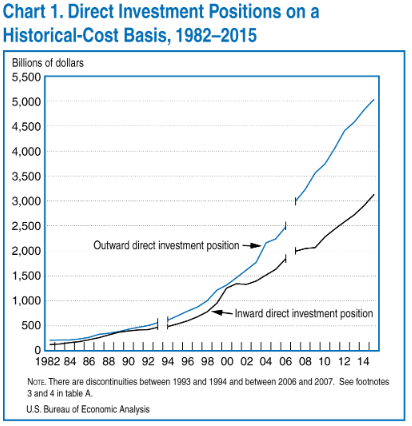
\includegraphics[width=110mm, height=80mm,clip, trim= 3mm 4mm 4mm 20mm]{DirectInvest_2015.png}
% \setlength\fboxsep{0pt}
 %\setlength\fboxrule{0.5pt}
 %\fbox{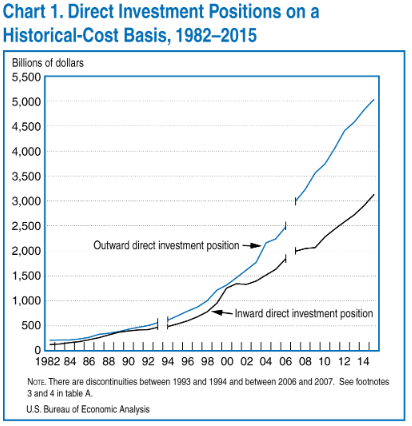
\includegraphics[width=120mm, height=75mm, clip, trim= 5mm 8mm 5mm 20mm]{DirectInvest_2015.png}}
 \end{center}
 \label{your-reference-key}
 \end{figure} 

The U.S. international tax rules are found primarily in subchapter N (sections 861 through 999) of the Internal Revenue Code, but scattered outside of subchapter N are some important international tax provisions, such as section 367 (reorganizations involving foreign corporations), section 482 (related party transactions), section 1248 (sales of the stock of foreign corporations), and sections 1291-1298 (passive foreign investment companies).  Importantly, the principles and rules you have learned in your other tax classes regarding the timing of an item of income or deduction, the tax classification (interest, dividend, or sale of goods or services), and the tax character (ordinary income or capital gain), do not cease to apply because one of the parties is foreign or the transaction occurs abroad.  In fact, because many types of income earned by foreigners, such as capital gains, are generally exempt from U.S. tax, these determinations are often more important for foreigners than domestic taxpayers.

%but The primary reason is the continued importance of cross-border trade and investment.  As U.S. individuals and firms venture outside of the United States to sell their labor, to manufacture and sell products, license their intangible property or invest their capital, the country in which these activities occur may tax the wages, revenues, royalties, or investment returns generated by these activities.  The United States may also tax those same returns. Foreign individuals and firms face similar tax issues when they carry on economic activities in the United States. 

							%Here: data on cross border trade and investment
							%Technical Considerations : Code /regs, etc
							% Important considerations:  affect investment choice and structure, pricing assets
	\section{Overview  Source and Residence Basis Taxation}
	
Most countries \margit{Source basis taxation applies to income arising in a country.} exert their taxing authority on two bases or types of jurisdictions: source and residence.  A country exercises \emph{source basis} tax jurisdiction over income arising within its borders that is earned by a foreign person, which can be an individual, corporate entity, or sovereign.  A dividend paid by a U.S. corporation, for example, is classified as U.S. source income, and if received by a foreign person, is generally subject to U.S. tax, even though the foreign person was never physically present in the United States.  The rationale behind source basis taxation is that the source country has provided the primary benefits, such as infrastructure, markets, and property rights,  to generate the income.    
	
Two distinct \margit{Foreign persons are taxed on a \emph{gross} basis on U.S. source investment income and on a net basis on U.S. source business income.} U.S. tax regimes apply to U.S. source income earned by foreign persons.  Foreign persons who earn only U.S. source passive or investment income such as dividends, rents, and royalties, are taxed at a flat 30\% rate (no deductions permitted).  In contrast, foreign persons who have a U.S. trade or business are taxed on the \emph{net}  U.S. source income (gross income reduced by allocable deductions) that is ``effectively connected'' with the U.S. trade or business at the same graduated rates applicable to U.S. persons. Gains from the sale of U.S. real property interests are taxed as effectively connected income. 

A country exerts \emph{residence basis} taxation \margit{Residence basis taxation applies to persons, including legal persons.} over persons on the basis of their legal status.  Persons (including legal persons such as corporations) subject to residence basis taxation are taxed on their worldwide income.  Under the ability-to-pay principle, residence basis taxation is justified on the grounds that both U.S. and foreign source income equally affect a person's ability to pay.  In addition, exempting foreign source could cause capital to flow abroad even if it could be more profitably invested in the United States.

The United States taxes its citizens, resident aliens, and corporations incorporated in one of the fifty states on a residence basis.  The United States, it should be noted, is unique among economically advanced nations in taxing its nonresident citizens on a residence basis and the foreign business income of its corporations. 

A U.S. person could easily avoid U.S. residence basis taxation merely by forming a foreign corporation and holding investment and business assets in the corporation.  Left unchecked, such a system could lead to a substantial reduction in U.S. tax revenue and an uneconomic skewing of investment and business capital.  To thwart such tax planning, the U.S. has enacted two anti-deferral regimes, the controlled foreign corporation and the passive foreign investment company regimes, under which U.S. shareholders of these foreign corporations are taxed currently on some or all of the corporations' current earnings regardless of whether the earnings are actually distributed to the shareholders (or are subject to an interest charge when the earnings are distributed).  Importantly, however, the business income of a controlled foreign corporation is generally not taxed by the United Sates until the income is remitted to the corporation's U.S. shareholder, typically the U.S. parent.  

The treatment of business profits earned by foreign subsidiaries of U.S.-based multinational corporations presents many policy and administrative challenges.  Some argue that such profits should be taxed currently at regular corporate rates (or a reduced rate) so that U.S. multinationals will not have a tax incentive to locate operations and jobs offshore.  Others argue that since most other developed countries do not tax the foreign business operations of their multinationals, if the United States taxed the offshore operations of its multinationals, the U.S. multinationals would be at a competitive tax disadvantage vis-a-vis their foreign counterparts.  

In recent years, U.S. multinationals and their foreign competitors have developed sophisticated tax structures that reduce and often eliminate any source basis taxation on business profits, leading to the rise of so-called \emph{stateless income}.  This development has caused much consternation among developed countries as their tax administrators see a marked drop in business tax revenues.  

In an effort to avoid the sting of the U.S. anti-deferral regimes, some U.S. multinationals have  \textit{inverted} their corporate structure by making the former U.S. parent a subsidiary of a new foreign parent, but without changing the identity of the shareholders.  Also, some recent public mergers between U.S. and foreign companies have resulted in inverted structures as well, much to the chagrin of some members of Congress and U.S. tax administrators.  Although there are U.S. tax provisions that attempt to discourage inversions, many commentators believe that they need to be strengthened.       

International double taxation arises when two or more countries assert tax jurisdiction over the same income or same persons.  For example, if a U.S. resident receives a dividend from a U.K. corporation and the U.K taxes the dividend, the dividend will be taxed twice, once by the United States on a residence basis and once by the United Kingdom on a source basis.   Double taxation is anathema to both taxpayers and governments: multiple layers of taxation can quickly become confiscatory, and if left unchecked, would significantly reduce cross-border trade and investment.  

To ameliorate double taxation, \margit{Double taxation is generally mitigated by the residence country ceding primary tax jurisdiction to the source country.   Source trumps residence.}the residence country generally cedes taxing primary jurisdiction to the source country.  The justification is that the source country is primarily responsible for the generation of the income, and source basis taxation should therefore take precedence. The United States unilaterally mitigates double taxation by allowing a credit for foreign taxes paid on foreign source income.  Other countries mitigate double taxation through a credit system, exemption of foreign source income, or a particular tax treaty provision.  Even if every country had the same double tax relief mechanism, however, double taxation would invariably arise because of different national definitions of residence, source, and the characterization of income.  

	\section{Overview of Income Tax Treaties}
	
To resolve these fundamental fiscal conflicts, countries enter into bi-lateral income tax treaties.  Treaties, which generally take precedence over domestic law, mitigate double taxation by providing rules of precedence when fiscal conflicts arise.  For example, a person who is a resident of more than one country--a U.S. green card holder residing in another country--could be subject to residence basis taxation by both the United States and his country of residence.  Tax treaties prevent this by establishing a single fiscal residence.  Treaties also often contain specific source rules and double tax relief provisions, the latter being especially important for persons residing in a country without a domestic foreign tax credit.   

Treaties \margit{Treaties lower source basis taxation and thereby increase the revenue of residence countries.}also aim to foster increased trade and investment by lowering source country taxation.  U.S. source dividends paid to a foreign treaty resident, for instance, are generally taxed at a maximum 15\% (or sometimes 5\% or 0\%) instead of 30\% under U.S. domestic law.  Also, income of a U.S. trade or business earned by a treaty resident is not taxed by U.S. unless the trade or business rises to the level of a \textit{permanent establishment}, which requires more substantive activities and presence than a trade or business.  By lowering source basis taxation, treaties in essence shift tax revenue from source countries to residence countries.  

Most tax treaties are based on the Organization of Economic Cooperation and Development (OECD) Model Tax Convention on Income and Capital and the detailed Commentaries, which are used in implementing and interpreting treaty provisions.  The OECD Model Treaty was first developed in 1958 and was based on the work of economists from the 1920's.\footnote{ The OECD was  formed in 1960 when 20 countries (the 18 members of the Organization for European Economic Cooperation, the United States, and Canada)  signed the OECD Convention, which endeavors to promote growth and improved standards of living for members, sound economic expansion of member countries, and expansion of world trade.  Since its founding the OECD has grown to include 34 members from around the world, with Chile, Estonia, Israel, and Slovenia becoming the most recent countries to join.}  

The United States has entered into over 60 income tax treaties, including treaties with almost all of its major trading and investment partners, and is continually expanding its treaty network.  The United States also has issued various model treaties, the most recent being the 2016 U.S. Model Treaty, which supersedes the 2006 Model.  The technical explanation is expected to be issued in 2017.  The model treaties are updated to reflect changes in U.S. tax policy.   

This book uses the U.S.-U.K.income tax treaty as its reference treaty. This treaty was signed in 2001 and came into force on March 31, 2003.  The U.S.-U.K. treaty is a treaty with a major trading partner and contains many provisions that specifically reflect recent U.S. international tax policy concerns.  The U.S.-U.K. treaty and the U.S. Treasury Technical Explanation of the Treaty are found in Appendix A.  I opted to use an actual tax treaty rather than either the OECD or U.S. Model Treaty mostly to avoid awkward phrasings such as ``X is a resident of a country with which the U.S. has tax treaty identical to the U.S. or OECD Model Treaty,'' or ``X is a resident of Treatyland.''  In addition, you can see how a particular treaty resolves specific conflicts that arise when two separate fiscal regimes meet.    

This rise of stateless income and the concern that unilateral responses by OECD members could result in double taxation  and increased tax uncertainty for cross-border investments led the OECD to address base erosion and profit shifting in the context of cross-border transactions.  In response to their findings, the OECD approved in 2013 the \emph{BEPS Action Plan}, which identified 15 action items that required new international standards.\footnote{OECD, Action Plan on Base Erosion and Profit Shifting, July 19, 2013, available at \url{http://www.oecd.org/tax/action-plan-on-base-erosion-and-profit-shifting-9789264202719-en.htm}}  Key action items were electronic commerce, hybrid mismatch arrangements, transfer pricing aspects of intellectual property, CFC rules, interest deductibility, and data collection.  Final reports on all items were finished in 2015 and endorsed by the G20 leaders.  Individual countries, including the United States, have already begun to implement some of the action items.\footnote{Recent developements and country-by-country trackers can be found in at the following links:   \url{http://www2.deloitte.com/global/en/pages/tax/articles/beps-country-scorecards.html}; \url{http://www.ey.com/GL/en/Services/Tax/OECD-base-erosion-and-profit-shifting-project} } We'll visit many of these topics throughout the semester.

 

\section{Overview of Text}
After examining the rules that classify persons as foreign or U.S. and legal entities as either partnerships or corporations, we will focus our study of U.S. international tax rules on two main areas: (1) \margit{\emph{Inbound} refers to the taxation of foreigners' U.S. investments and activities, and \emph{Outbound} to the taxation of the foreign operations of U.S. persons} the taxation of foreigners investing and doing business in the United States (source basis tax jurisdiction); and (2) the taxation of U.S. persons investing and doing business abroad (residence basis jurisdiction), including the U.S. anti-deferral regimes, \emph{i.e.}, the controlled foreign corporation and passive foreign investment provisions, and the foreign tax credit regime, the domestic mechanism the United States employs to coordinate overlapping tax jurisdiction.  Tax treaty provisions are integrated throughout with the relevant domestic provisions.  We also examine section 482, which requires related parties to deal with each other on an arm's-length basis.  This important provisions applies to both U.S. and foreign taxpayers.  

Along the way, we will also examine some proposals to modify the current U.S. international tax regime, as Congress and Treasury grapple on one hand with concerns of U.S.-based multinationals that the U.S. tax system places them at a competitive disadvantage vis-a-vis their foreign competitors and on the other that our current tax system favors foreign investment over U.S. investment thus encouraging jobs and capital to move oversees.  It is virtually certain that we'll see in 2017 some of the most signficant changes to the U.S. international tax regime in the last 50 years.  

Like other parts of the Internal Revenue Code, the international tax provisions reflect many compromises among competing objectives such as fairness vis-a-vis U.S. taxpayers, revenue raising, administration, and encouraging foreign investment. Because these objectives are sometimes contradictory, the U.S. international tax rules are not entirely consistent or simple.  But that makes the course stimulating and challenging and the field an interesting and potentially lucrative one to work in.  

	\begin{framed}
		Last revised:  Jan. 10, '17
			\end{framed}

 
		 
\chapter{Residence, Nationality, and U.S. Tax Jurisdiction}
	\section{Citizens and Residence Basis Taxation}
		\crt{1}{1.1-1(b) and (c)}{1(1), 1(4), and 1(5); 4; and 23(1) and (2) (skim only)}

\intro{This chapter discusses the tax residence of individuals and legal entities.  It focuses first on U.S. citizens and explores the long-standing U.S. position of taxing its citizens (and resident aliens) on their worldwide income, regardless of actual physical residence or economic contacts with the United States.  It then addresses \S 7701(b), which determines when a foreign national is treated as a U.S. resident.  Next, the rules regarding the tax residence of legal entities, such as partnerships and corporations, are covered, including the check-the-box regulations (Reg.\@ \S\S 301.7701-1, 2, and 3), which are without doubt one of most important developments in the U.S. international tax regime in the last twenty years.  Finally, the residence of trusts and estates is briefly addressed.}

%\addcontentsline{toc}{section}{\protect\numberline{}Taxation of Citizens and Residents under U.S. Law} 
%	\begin{center}
			\subsection{Taxation of Citizens and Residents under U.S. Law}
		%\textbf{Taxation of Citizens and Residents under U.S. Law}
%			\end{center}

The notion of residence is one of the cornerstones of the U.S. international tax regime.  U.S. citizens, including dual citizens, and resident aliens are generally taxed on a residence basis, regardless of their actual physical residence, domicile, or economic contacts with the United States. Thus, \margit{The United States is the only country that taxes its non-domiciled citizens and resident aliens on a residence basis.}  all income, regardless of its geographic origin, is subject to U.S. income tax.  \emph{Cook v.\ Tait}, below, recognizes that the constitutional power to levy income taxes on U.S. citizens (and by extension resident aliens) is not tethered at the U.S. border.  Nonresident aliens, in contrast, are taxed on a source basis, and income of a nonresident that does not have any nexus to the United States (foreign source income) is not taxed by the United States.  Because of the fundamental distinction between residence and source basis taxation, one of the first determinations you must make as a tax advisor is your client's tax residence.

A notable exception to residence basis taxation is found in  \S 911, which permits a citizen or resident alien who resides and earns income abroad to elect to exclude from U.S. tax a portion of his foreign earned income (up to \$100,800 for 2015) and other non-cash benefits.  

Aware that the lure of source basis taxation may be an irresistible inducement to well-heeled citizens and resident aliens to renounce their U.S. citizenship or residence, Congress has enacted special income, gift, and estate provisions intended to discourage persons from renouncing their U.S. citizenship or long-term residency solely for tax purposes.  Under \S 877A, certain citizens and long-term resident aliens who renounce their citizenship or abandon their U.S. residency are subject to tax on the unrecognized gain in their property.  In addition, they are also subject to a modified U.S. estate and gift tax regime.  Sections 911 and 877A are discussed below in Chapter 8.   

The Constitution imposes virtually no limits on Congress's power to tax income.  Article I, Section 8, Clause 1 of the Constitution grants Congress the ``the power To Lay and collect Taxes, Duties, Imposts, and Excises..."  Although ``direct taxes" must be apportioned among the states in proportion to their population (Article I, Section 9, Clause 4), the Sixteenth Amendment abolished the apportionment requirement for ``taxes on incomes, from whatever source derived..."

The word ``source" in the Sixteenth Amendment refers to the economic origin or source of the income, \textit{e.g.}, wages or property, and not to geographic source.  Early Treasury regulations extended the income tax to encompass the income of U.S. citizens and resident aliens arising from any geographic source.  The validity of this regulation, and the U.S. constitutional power to tax the worldwide income of its citizens and resident aliens, even those with a foreign domicile, was affirmed in \textit{Cook v. Tait} 

% tie breaker whats subjective what easy to change
\addcontentsline{toc}{section}{\protect\numberline{}Cook v.\ Tait} \begin{select}
\caseart{Cook v.\ Tait}{ 265 U.S. 47 (1924)}{Justice McKennna} delivered the opinion of the Court.

\ldots The tax was imposed under the Revenue Act of 1921, which provides by \S210 (42 Stat. 227, 233): ``That, in lieu of the tax imposed by section 210 of the Revenue Act of 1918, there shall be levied, collected, and paid for each taxable year upon the net income of every individual a normal tax of 8 per centum \margit{Note the maximum federal tax rate.}of the amount of the net income in excess of the credits provided in section 216: Provided, That in the case of a citizen or resident of the United States the rate upon the first \$4,000 of such excess amount shall be 4 per centum.''\footnote[1]{\ldots [R]egulation, No. 62 \ldots provides in Article 3: ``Citizens of the United States except those entitled to the benefits of section 262 [\ldots] wherever resident, are liable to the tax. It makes no difference that they may own no assets within the United States and may receive no income from sources within the United States. Every resident alien individual is liable to the tax, even though his income is wholly from sources outside the United States. Every nonresident alien individual is liable to the tax on his income from sources within the United States.''} 

Plaintiff is a native citizen of the United States and was such when he took up his residence and became domiciled in the City of Mexico.\ldots\ 

The question in the case \ldots\ [is] whether Congress has power to impose a tax upon income received by a native citizen of the United States who, at the time the income was received, was permanently resident and domiciled in the City of Mexico, the income being from real and personal property located in Mexico.
 
Plaintiff assigns against the power not only his rights under the Constitution of the United States but under international law, and in support of the assignments cites many cases. It will be observed that the foundation of the assignments is the fact that the citizen receiving the income, and the property of which it is the product, are outside of the territorial limits of the United States. \margit{Is this what Cook argued?}These two facts, the contention is, exclude the existence of the power to tax. Or to put the contention another way, as to the existence of the power and its exercise, the person receiving the income, and the property from which he receives it, must both be within the territorial limits of the United States to be within the taxing power of the United States. The contention is not justified, and that it is not justified is the necessary deduction of recent cases. \ldots 
%%In United States v.\ Bennett, 232 U.S. 299, the power of the United States to tax a foreign built yacht owned and used during the taxing period outside of the United States by a citizen domiciled in the United States was sustained. The tax passed on was imposed by a tariff act, \ldots\ but necessarily the power does not depend upon the form by which it is exerted.
 \ldots
%%It will be observed that the case contained only one of the conditions of the present case, the property taxed was outside of the United States. In United States v.\ Goelet, 232 U.S. 293, the yacht taxed was outside of the United States but owned by a citizen of the United States who was ``permanently resident and domiciled in a foreign country.'' It was decided that the yacht was not subject to the tax---but this as a matter of construction. Pains were taken to say that the question of power was determined ``wholly irrespective'' of the owner's ``permanent domicile in a foreign country.'' And the Court put out of view the situs of the yacht. That the Court had no doubt of the power to tax was illustrated by reference to the income tax laws of prior years and their express extension to those domiciled abroad. The illustration has pertinence to the case at bar, for the case at bar is concerned with an income tax, and the power to impose it. 

We may make further exposition of the national power as the case depends upon it. It was illustrated at once in United States v.\ Bennett by a contrast with the power of a State. It was pointed out that there were limitations upon the latter that were not on the national power. The taxing power of a State, it was decided, encountered at its borders the taxing power of other States and was limited by them. There was no such limitation, it was pointed  out, upon the national power; and the limitation upon the States affords, it was said, no ground for constructing a barrier around the United States ``shutting that government off from the exertion of powers which inherently belong to it by virtue of its sovereignty.''
 
The contention was rejected that a citizen's property without the limits of the United States derives no benefit from the United States. The contention, it was said, came from the confusion of thought in ``mistaking the scope and extent of the sovereign power of the United States as a nation and its relations to its citizens and their relations to it.'' And that power in its scope and extent, it was decided, is based on the presumption that government by its very nature benefits the citizen and his property wherever found, and that opposition to it holds on to citizenship while it ``belittles and destroys its advantages and blessings by denying the possession by government of an essential power required to make citizenship completely beneficial.'' In other words, the principle was declared that the government, by its very nature, benefits the citizen and his property wherever found and, therefore, has the power to make the benefit complete. \margit{The benefits and burden rationale.}Or to express it another way, the basis of the power to tax was not and cannot be made dependent upon the situs of the property in all cases, it being in or out of the United States, and was not and cannot be made dependent upon the domicile of the citizen, that being in or out of the United States, but upon his relation as citizen to the United States and the relation of the latter to him as citizen. The consequence of the relations is that the native citizen who is taxed may have domicile, and the property from which his income is derived may have situs, in a foreign country and the tax be legal---the government having power to impose the tax.
 
Judgment affirmed. 
\end{select}

	\addcontentsline{toc}{section}{\protect\numberline{}Comments} 
			\begin{center}
		\textbf{\textit{Comments}}
			\end{center}

\begin{enumerate}
	\item

The  \textit{Cook} court invokes the benefits and burden rationale to support its holding.  Under the benefits principle, a person is taxed (the burden) in order to pay for the services (the benefits) provided by the government.  The court did not consider the question of whether the benefits provided by the U.S. government to nonresident citizens are the same as those provided to resident citizens.  A moment's reflection should be sufficient to answer that question in the negative.  Logically extended, the benefits rationale would at least require different tax rates for foreign income and U.S. income.  Perhaps the benefits rationale can be salvaged if one views the minimum benefit provided to all citizens and resident aliens is the right return to and live in the United States.  Finally, the benefits principle of taxation is incompatible with the notion that an aim of government is to redistribute goods and services to those who do not have the means to purchase them in the market.    

Under the more modern ability-to-pay principle, the tax burden should be borne in relation to a person's ability to pay as measured by his income.  Since \$100 of foreign income and \$100 of U.S. income both equally increases a person's ability to pay, both should be included in the tax base.  In addition, including foreign income in the tax base ensures that capital is allocated efficiently.  If foreign income were exempt from tax, U.S. persons would have a tax incentive to shift capital abroad.  

The U.S. tax system departs significantly from the ability-to-pay principle by deferring tax on the business income of the foreign subsidiaries of U.S. multinationals until the income is remitted to the U.S. parent.  This issue, and the U.S. anti-deferral regimes that have been enacted to prevent abusive use of foreign corporation by U.S. persons, is explored more fully below in Chapters 7, 10, and 11.

The benefits and burden principle may still have relevance if it is viewed as jurisdiction principle.  A wealthy foreigner clearly has more ability to pay than a U.S. pauper, but if the foreigner has no economic nexus to the United States, he pays no U.S. tax.  Could the United States tax wealthy foreigners with no nexus to the United States?  Such a regime would certainly raise due process concerns.  And if the United States implemented such a regime, it is certain that other countries would follow, potentially leading to a tax war. But more fundamentally, we do not tax such persons because they have not received any economic benefit from the United States.  

	\item
	Some scholars have questioned U.S. citizenship taxation on the basis that since it imposes tax and compliance barriers it may undermine the important value of free movement.  It may discourage the emigration of talented foreigners and thereby place the United States at a competitive disadvantage.  \textit{See} Ruth Mason, \textit{Citizenship Taxation}, 89 S. Cal. L. Rev. 169  (2016).  
\end{enumerate}

%	\addcontentsline{toc}{section}{\protect\numberline{}Treaties and Citizens} 
%	\begin{center}
%		\textbf{Tax Treaties and U.S. Citizens and Residents}
%			\end{center}
\subsection{Tax Treaties and U.S. Citizens and Residents}

A tax treaty bestows tax benefits--generally in the form of reduced source basis taxation--only to a treaty \emph{resident}. Article 1(1).  To qualify for treaty benefits, a person (including legal persons) must be a \emph{resident} as determined in Article 4; a legal person, such as a corporation, must also be a \emph{qualified person} under Article 23.  Article 23(1) and (2).  \margit{Residence is defined in Article 4.  Legal entities must also be qualified persons under Article 23.} 

An individual is a treaty resident if he is subject to tax by one of the contracting states ``by reason of his domicile, residence, citizenship \ldots or any other criterion of a similar nature.''  Article 4(1).  Although a U.S. citizen or resident alien will generally qualify as a U.S. treaty resident, Article 4(2), however, requires a U.S. citizen or resident alien with a ``green card'' to satisfy two additional requirements to be a Treaty resident.  First, he must have a ``substantial presence, permanent home, or habitual abode in the United States''; and second, he must not be treated as a treaty resident under any other U.K. treaty with a third country.  Article 4(2).  Consequently, a U.S. citizen or green card holder with minimal physical presence or economic connections to the United States is not a resident under the Treaty.  The Technical Explanation to Article 4(2) states that the second requirement prevents a citizen or resident alien from choosing the (potentially superior) benefits of the Treaty over those of the treaty between the United Kingdom and his foreign country of residence.  

The United States generally negotiates to extend treaty benefits to U.S. citizens and green card holders wherever resident.  This is beneficial to the United States as reducing source basis taxation generally increases the tax revenues of the residence country.  

To illustrate, assume a U.S. citizen whose marginal tax rate is 35\%, receives \$100 of interest from a U.K. corporation that would be taxed at 30\% by the United Kingdom but is taxed at 0\% under Article 11(1) of the Treaty.  If the Treaty did not apply, the United States would also tax the \$100 but would grant a credit for the 30\% U.K. tax paid leaving the U.S. fisc with a residual \$5--\$35 U.S. tax liability less a credit of \$30 of U.K. tax.  As a result of the Treaty, the U.K. tax rate is 0\%, and United States now collects the entire \$35 for an increase in U.S. tax revenues of \$30.  See Example 1.

	\begin{framed}
		\begin{center}
				\textsc{\textbf{Example 1:  Treaties Shift Revenues from Source to Residence Countries}}\\
		\end{center}
P, a U.S. citizen whose marginal tax rate is 35\%, receives  \$100 of interest from a U.K. corporation.  The U.K. tax rate in the absence of the Treaty is 30\%.  Assuming that P can credit the U.K. tax against his (pre-credit) U.S tax liability of \$35, P pays an additional \$5 to the United States, which receives only \$5.  If the Treaty applies, however, the U.K. tax rate is 0\%, and P pays \$35 to the United States.  P pays of total of \$35 in either case, but the Treaty shifts \$30 of revenue from the United Kingdom (source country) to the United States (residence country). 

 	\begin{center}
	  \begin{tabular}{l c c}
  		& No Treaty & Treaty\\
  	\hline
 		 Taxable Income & 100 & 100 \\
  		\ \ \ US Tax (Pre-credit) & 35 & 35 \\
 		 Less credit for U.K. Tax & (30) & (0) \\
  		Residual U.S. Tax & 5 & 35 \\
  		\hline
    		\end{tabular}
   	\end{center} 
   		\end{framed}
Our treaty partners, such as the United Kingdom, however, are generally not so keen to extend treaty benefits to resident aliens or U.S. citizens residing in third countries.  Because most of our treaty partners generally do not tax the worldwide income of their nonresident citizens, any source basis tax concession given by the United States to, for instance, a U.K. citizen residing in Mexico and not subject to U.K. tax on his worldwide income, would not affect U.K. tax revenues.  Assume that a U.K. citizen residing in Mexico receives a royalty for the use of a patent in the United States that is subject to a 30\% U.S. withholding tax.  If the U.K. citizen were able to use the Treaty to reduce the U.S. tax rate to 0\%, the United States would forego \$30 of revenue, but because the United Kingdom does not tax the non-U.K. income of its non-domiciled citizens, U.K. tax revenues would remain unchanged.  Thus, if the United Kingdom were to agree to give up source basis taxes on U.S. citizens and residents residing in third countries, its tax revenues from U.S. persons would decrease, but its tax revenues from its nonresident citizens would remain unchanged even with a reciprocal U.S. concession. 

	
	\section{Dual Citizens}
	
U.S. citizenship can be acquired in many ways: being born in the United States, becoming a naturalized citizen through marriage or residence in the United States, or being born outside of the United States to parents who are U.S. citizens.  A citizen retains his citizenship regardless where he subsequently resides, unless it is renounced.  Many citizens who were born abroad, have resided abroad their entire lives, and possess citizenship of another country may not be aware of their US. citizenship and the U.S. fiscal responsibilities that accompany it.  

A dual citizen of the United States and another country is also subject to residence basis taxation by the United States, unless he renounces his citizenship.  In Rev. Rul. 75-82, 1975-1 C.B. 5, the IRS ruled that a naturalized U.S. citizen who was born in Canada and eventually reestablished Canadian residence did not lose his U.S. citizenship solely by returning to Canada.  In addition, he continued to remain subject to U.S. tax.
\begin{quote}
Since the mere act of returning to and residing in Canada is not one of the acts described in 8 
U.S.C. section 1481 by which United States nationality is lost, and since the individual in the instant case had never performed any of the acts by which United States nationality is lost, he remained a United States citizen when he returned to Canada after attaining majority. Accordingly, he is not relieved of the duty incumbent on United States citizens of filing Federal income tax returns.
\end{quote}

Dual citizens are subject to overlapping residence tax claims by both countries.  The domestic law of each country rarely will provide complete relief against overlapping dual residence taxation, and in the absence of a tax treaty, double taxation will inevitably arise. 

Tax treaties \margit{To eliminate residence basis taxation by two countries, treaties provide for a single tax residence.}mitigate the problem of dual residence taxation by employing a series of tie breaker rules that generally result in the determination of a \emph{single} country of tax residence.  Under Article 4(4), a dual resident is considered to be a resident of the country in which he has a permanent home, where his personal and economic relations are closer, where he maintains a habitual abode, or where he is a national.  These tests are applied in order, so for example, if a dual resident has a permanent home in only one country, he will be a resident of that country regardless of his economic nexus with either country or his nationality.       

To protect residence basis taxation of its citizens residing abroad, the United States generally reserves the right pursuant to the so-called ``savings clause''--Article 1(4)--to tax its citizens and resident aliens regardless of any treaty benefits to which they otherwise may be entitled.  \margit{Under the savings clause, a U.S. citizen cannot generally use the Treaty to reduce U.S. tax.} Thus, even if a U.S. citizen is treated as a U.K. resident under Article 4(4), the savings clause would prevent him from using the Treaty to lower U.S. tax.  As there are almost no rules without exceptions, Article 1(5)(a) and (b) exempt certain narrow categories of income and individuals from the savings clause.\footnote{For instance, a U.S. citizen who is a U.K. resident is not subject to U.S. tax on U.S. social security benefits. Articles 1(5)(a) and 17(3).} But, you may ask yourself, wouldn't a U.S. citizen who's also a U.K. resident potentially be subject to double taxation? The answer is yes, but Article 24(6) of the Treaty coordinates overlapping fiscal claims to ameliorate possible double taxation.     

  \addcontentsline{toc}{section}{\protect\numberline{}Citizenship Regained} 
  \begin{center}
		\textbf{Citizenship Regained}
			\end{center}

If a U.S. citizen has lost or renounced his citizenship and has it restored retroactively, how should he be taxed during the period he was not treated as a U.S. citizen and did not reside in the United States or avail himself of any benefits of citizenship?  Resolving this issue raises questions about the underlying basis on which U.S. residence basis tax is levied.  

In \textit{Felix Benitez Rexach v.\ U.S.}, 390 F.2d 631 (1st. Cir. 1968), \emph{cert.\ denied}, 393 U.S. 833 (1968), Rexach, a U.S. citizen who resided in the Dominican Republic and worked on large scale construction projects, renounced his citizenship in 1958.  When then-Dictator Trujillo was assassinated in 1961, Rexach had a change of heart.  He successfully argued that his renunciation was coerced and had his U.S. citizenship restored \textit{ab inicio}.  After restoring his citizenship, the United States then sued Rexach for income taxes during these years.  Rexach argued that  ``since the United States `owed' him, or apparently owed him, no citizen's protection, he, in turn, owed no tax."  The court rejected Rexach, stating:

\begin{quote} 

While there is language in Cook v.\ Tait, supra, indicative that these are reciprocal obligations, the Court also observed that ``government by its very nature benefits the citizen * * *.'' \ldots We cannot agree that the reciprocal obligations are mutual, at least in the sense that taxpayer contends.  It is sufficient that the government's stem from its de jure relationship without regard to the subjective quid pro quo in any particular case. We will not hold that assessment of benefits is a prerequisite to assessment of taxes.\ldots\footnote{\textit{Felix Benitez Rexach v.\ U.S.}, 390 F.2d 631, 632 (1st. Cir. 1968), \emph{cert.\ denied}, 393 U.S. 833 (1968)}

\end{quote}

 A related case, \textit{U.S. v.\ Lucienne d'Hotelle de Benitez Rexach}, 558 F.2d 37 (1st.\ Cir.\ 1977), involved Lucienne, Felix's wife.  Lucienne was born in France and become a naturalized citizen in 1942.  She returned to France in 1946 and remained a French resident until May 20, 1952. During that time, \S 404(b) of the Nationality Act of 1940 provided that naturalized citizens who returned to their country of birth and resided there for three years lost their American citizenship. Her U.S. passport was renewed in 1947 and 1949, but her citizenship was stripped on May 20, 1952 pursuant to \S 404(b).  The successor statute to \S404(b) was held to be unconstitutional in \textit{Schneider v. Rusk}, 377 U.S. 163 (1964), and its holding was applied retroactively.  Because the Dominican Republic was a community property state, Lucienne legally owned one-half of Felix's income, and the U.S. government sued to collect tax on her share.  Lucienne had accepted her loss of citizenship and never applied to have it reinstated.
 
The First Circuit upheld the government's position that she was liable to U.S. taxes for the years 1949 (the date her citizenship was lost under \S 404(b)) through 1952 (the date a certificate of loss of nationality was issued to her) stating that ``...the balance of the equities mandates that back income taxes be collectible for periods during which the involuntarily expatriated persons affirmatively exercised a specific right of citizenship."  In Lucienne's case, the specific right of citizenship was her possession and use of an American passport.  For the post-1952 years, however, the court said \textit{in dicta} that the government should not be allowed to tax her:  

\begin{quote}
Although estoppel is rarely a proper defense against the government, there are instances where it would be unconscionable to allow the government to reverse an earlier position. \ldots This is one of those instances. Lucienne cannot be dunned for taxes to support the United States government during the years in which she was denied its protection. \ldots Here, Lucienne severed her ties to this country at the direction of the State Department. The right hand will not be permitted to demand payment for something which the left hand has taken away.\footnote{\textit{U.S. v.\ Lucienne d'Hotelle de Benitez Rexach}, 558 F.2d 37, 43 (1st.\ Cir.\ 1977).}
\end{quote}

Why was Felix taxed during his period of non-citizenship but Lucienne was not?  Should the basis on which citizenship was lost and restored matter if it is restored retroactively? If such persons should not be taxed because they did not receive any benefits of citizenship from the United States during the period of non-citizenship, then could it be argued that the foreign source income of U.S. persons residing abroad should also not be taxed or taxed at a lower rate?  Does a nonresident citizen receive the same benefits and protections as a resident citizen, especially with respect to property that is located abroad?  Can \S911 be construed as a partial attempt to implement a modified benefits principle for nonresident citizens? 

In addition to income taxes, the United States also subjects its residents and citizens to U.S. gift, estate, and generation skipping taxes on the worldwide transfers of property and worldwide estates.  The international implications of these taxes are discussed below in Chapter (  ).  Nonresidents, as specially defined for gift and estate tax purposes, are also subject to U.S. gift and estate taxes but generally only with respect to transfers of U.S. situs property.  Thus, a former citizen who regains his U.S. citizenship must not only determine whether he will be subject to income tax on a residence basis while an expatriate, but also whether he will be subject to U.S. gift or estate tax on a residence basis while an expatriate.

%\addcontentsline{toc}{section}{\protect\numberline{}Felix Benitez Rexach v.\ U.S.}
%\begin{select} \caseart{Felix Benitez Rexach v.\ United States}{ 390 F.2d 631 (1st. Cir. 1968), \emph{cert.\ denied}, 393 U.S. 833 (1968)}{Aldrich, Chief Judge.}\\
%\ldots 
%Felix Benitez Rexach, \ldots, an American citizen,\ldots left Puerto Rico [in 1944] and became a resident of the Dominican Republic, where he remained until 1961. In July 1958 he executed a written renunciation of his American citizenship before a United States consulate official in the Dominican Republic pursuant to the Immigration and Nationality Act of 1952, 8 U.S.C. \S 1481(a)(6). A certificate of loss of nationality was duly approved by the Department of State. On July 26 taxpayer was decreed to be a citizen of the Dominican Republic. Thereafter, he naturally suffered certain losses of status and benefits as a consequence of being declared a non-resident alien of the United States. 

%Taxpayer was engaged in large scale contracting activities in the Dominican Republic in connection with the then dictator, Trujillo. In 1961 Trujillo was assassinated. \margit{Another example of the importance of choosing wisely your friends and business associates.}The following year taxpayer applied for an American passport, claiming that his 1958 renunciation was not voluntary but had been compelled, against his will, by economic pressure and physical threats that he feared to resist. The United States Consul denied his application, and taxpayer appealed to the Department of State. The Board of Review on the Loss of Nationality took taxpayer's testimony and accepted it, as a result of which his certificate of loss of nationality was cancelled, and his passport application granted. There followed the present chapter. The [CIR] assessed taxpayer with an income tax on account of income earned in the Dominican Republic during the years following his renunciation of citizenship, alleged to be due because of his continued American citizenship. Cook v.\ Tait\ldots 

%Taxpayer concedes that as a matter of law he is precluded by the record from claiming that he ever ceased to be a United States citizen, and concedes that during the period in question he was a de jure citizen. However, he says that he was not a ``de facto'' citizen.  
%\begin{quote}``Appellant does not claim that his citizenship was lost as a result of the renunciation, but that as a result of the determination of the Secretary of State and consequent issue of the Certificate of Loss of Nationality, the United States was freed of its obligations to him as a citizen and he in fact lived and existed as an alien to the United States during the period in question.''
%\end{quote}
%He concludes that since the United States ``owed'' him, or apparently owed him, no citizen's protection, he, in turn, owed no tax. 

%While there is language in Cook v.\ Tait, supra, indicative that these are reciprocal obligations, the Court also observed that ``government by its very nature benefits the citizen * * *.'' \ldots We cannot agree that the reciprocal obligations are mutual, at least in the sense that taxpayer contends.  \margit{What's left of the benefit and burden rationale?}It is sufficient that the government's stem from its de jure relationship without regard to the subjective quid pro quo in any particular case. We will not hold that assessment of benefits is a prerequisite to assessment of taxes.\ldots
%\end{select}

%\begin{select}
%\addcontentsline{toc}{section}{\protect\numberline{}U.S. v.\ Lucienne Benitez Rexach}
%\caseart{United States v. Lucienne D'Hotelle de Benitez Rexach }{558 F.2d 37 (1st.\ Cir.\ 1977)}{Ingraham, Circuit Judge.}\\
%\ldots
%\begin{center}
%\textbf{FACTS} \\
%\end{center}
%Lucienne D'Hotelle was born in France in 1909. She became Lucienne D'Hotelle de Benitez Rexach upon her marriage to Felix in San Juan, Puerto Rico in 1928. She was naturalized as a United States citizen on December 7, 1942. The couple spent some time in the Dominican Republic, where Felix engaged in harbor construction projects. Lucienne established a residence in her native France on November 10, 1946 and remained a resident until May 20, 1952. During that time \S 404(b) of the Nationality Act of 1940 \ldots provided that naturalized citizens who returned to their country of 
%birth and resided there for three years lost their American citizenship. On November 10, 1947, after Lucienne had been in France for one year, the American Embassy in Paris issued her a United States passport valid through November 9, 1949. Soon after its expiration Lucienne applied in Puerto Rico for a renewal. By this time she had resided in France for three years. Nevertheless, the Governor of Puerto Rico renewed her passport on January 20, 1950 for a two year period beginning November 10, 1949. Three months after the expiration of this passport, Lucienne applied to the United States 
%Consulate in Nice, France for another one. On May 20, 1952, the Vice-Consul there signed a Certificate of Loss of Nationality, citing Lucienne's continuous residence in France as having automatically divested her of citizenship under \S 404(b). Her passport from the Governor of Puerto Rico was confiscated, cancelled and never returned to her. The State Department approved the certificate on December 23, 1952. Lucienne made no attempt to regain her American citizenship; neither did she affirmatively renounce it.
 
%In October 1952 the Dominican Republic (then controlled by the dictator Rafael Trujillo) extended citizenship to Lucienne retroactive to January 2, 1952. \margit{How old were Felix and Lucienne when they married?} Trujillo was assassinated in May 1961. The provisional government which followed revoked Lucienne's citizenship on January 20, 1962. On June 5, 1962 the French government issued her a passport. 

%For the years 1944 to 1958, Felix earned millions of dollars from harbor construction in the Dominican Republic. He was aided by Trujillo's favor and by his own undeniable skills as an engineer. Felix, an American citizen since 1917,\footnote[3]{Felix was born in Puerto Rico on March 27, 1886.\ldots\ [, and he lost his U.S. citizenship in 1958.]  However, the Board of Review on the Loss of Nationality later determined that the events which led to denaturalization were the result of coercion by Trujillo. It adjudged the denaturalization to be void \emph{ab initio}.\ldots} was sued by the United States for income taxes. The court held that Lucienne had a vested one-half interest in Felix's earnings under Dominican law, which established that such income was community property. Since the law of the situs where the income was earned determined its character, Felix could be sued only for his half of the earnings. \ldots
% 
%Predictably, the United States eventually sought to tax Lucienne for her half of that income. Whether by accident or design, the government's efforts began in earnest shortly after the Supreme Court invalidated  the successor statute \ldots to \S 404(b). In Schneider v.\ Rusk, 377 U.S. 163 (1964), the Court held that the distinction drawn by the statute between naturalized and native-born Americans was so discriminatory as to violate due process. In January 1965, about two months after this suit was filed, the State Department notified Lucienne by letter that her expatriation was void under Schneider and that the State Department considered her a citizen. Lucienne replied that she had accepted her denaturalization without protest and had thereafter considered herself not to be an American citizen. 

%Lucienne died on January 18, 1968. During her lifetime, Felix, as administrator of the marital community, retained and administered the community property, including Lucienne's share of the income earned in the Dominican Republic. \margit{Nice guy.  An example of the importance of choosing wisely your spouse.} Upon her death Felix did not return her share to the estate, but retained it. \ldots 

%The district court found that Lucienne was liable for taxes on her half of Felix's income from 1944 through November 9, 1949\ldots.  

%The United States appealed the denial of liability for the period November 10, 1949 to May 20, 1952.\ldots

%\begin{center}
%\textbf{LUCIENNE'S CITIZENSHIP} \\
%\end{center}

% The government contends that Lucienne was still an American citizen from her third anniversary as a French resident until the day the Certificate of Loss of Nationality was issued in Nice. This case presents a curious situation, since usually it is the individual who claims citizenship and the government which denies it. But pocketbook considerations occasionally reverse the roles.\ldots\ The government's position is that under either Schneider v.\ Rusk, supra, or Afroyim v.\ Rusk, 387 U.S. 253 (1967), the statute by which Lucienne was denaturalized is unconstitutional and its prior effects should be wiped out. Afroyim held that Congress lacks the power to strip persons of citizenship merely  because they have voted in a foreign election. The cornerstone of the decision is the proposition that intent to relinquish citizenship is a prerequisite to expatriation. 

%Section 404(b) would have been declared unconstitutional under either Schneider or Afroyim. The statute is practically identical to its successor, which Schneider condemned as discriminatory. \ldots 

%We think the principles governing retrospective application dictate that either Schneider or Afroyim apply to this case. \ldots\ This circuit has applied Afroyim retroactively.\ldots

%\ldots However, the district court went too far in viewing the equities as between Lucienne and the government in strict isolation from broad policy considerations which argue for a generally retrospective application of Afroyim and Schneider to the entire class of persons invalidly expatriated. \ldots\ The rights stemming from American citizenship are so important that, absent special circumstances, they must be recognized even for years past. Unless held to have been citizens without interruption, persons wrongfully expatriated as well as their offspring might be permanently and unreasonably barred from important benefits.\footnote[6]{For example, if expatriation was void \emph{ab initio}, the reinstated citizen will have the satisfaction of knowing that children born in the interim will have the right to become citizens. 8 U.S.C. \S\S1431, 1433, 1434.\ldots\ } Application of Afroyim or Schneider is generally appropriate. 

%Of course, American citizenship implies not only rights but also duties, not the least of which is the payment of taxes. Cook v.\ Tait.\ldots\ And were Schneider or Afroyim used to compel payment of taxes by all persons who mistakenly thought themselves to have been validly expatriated, the calculus favoring retrospective application might shift markedly. We do think that the balance of the equities mandates that back income taxes be collectible for periods during which the involuntarily expatriated persons affirmatively exercised a specific right of citizenship. This is precisely the position taken by the [IRS in Rev. Rul. 75-357].  As to such periods, neither the government nor the expatriate can be said to have relied upon the constitutionality of \S404. Since the expatriate in fact received benefits of citizenship, the equities favor the imposition of federal income tax liability. Cf.\ Benitez Rexach v.\ United States, \ldots. 
% 
%We now focus upon Lucienne's status. The years for which the government sought to collect taxes 
%can be divided into three discrete periods: 1944 through November 9, 1949; November 10, 1949 
%through May 20, 1952; and May 21, 1952 through 1958. The district court's ruling that 
%Lucienne was liable for taxes during the first period is not appealed. The district court refused to 
%distinguish between the two remaining periods. 
%During the interval from late 1949 to mid-1952, Lucienne was unaware that she had been
%automatically denaturalized. In fact, she applied for, obtained and used an American passport for 
%most of that period. On the passport application she stated that her travel outside the United States 
%had consisted of ``vacations," and her signature appeared below an oath that she had neither been 
%naturalized by a foreign state nor declared her allegiance to a foreign state. Her subsequent 
%application on February 11, 1952, which was eventually rejected, included an affidavit in which she 
%stated that her mother's death and other business obligations caused her to remain in France. 
%Ironically, on that same application, the following line appears: 
%\begin{quote}``I (do/do not) pay the American Income Tax at \_\_\_\_\_ ." 
%\end{quote}
%Lucienne scratched out the words ``do not" and filled in the blank with ``San Juan, Puerto Rico." 
%As late as February 1952 Lucienne regarded herself as an American citizen and no one had 
%disabused her of that notion. The Vice Consul reported that Lucienne had told him ``she was 
%advised (by the State Department) that she could remain in France without endangering her 
%American citizenship." 

%Fairness dictates that the United States recover income taxes for the period November 10, 1949 to 
%May 20, 1952. Lucienne was privileged to travel on a United States passport; she received the 
%protection of its government. 

%Although the government has not appealed the decision with respect to taxes from mid-1952 
%through 1958, the district court was presented with the issue. We wish to explain why the 
%government should be allowed to collect taxes for the two and one-half year interval but not for the 
%subsequent period. The letter from Lucienne to the Department of State official in 1965, which 
%appears in English translation in the record, states that after the Certificate of Loss of Nationality, ``I 
%have never considered myself to be a citizen of the United States." We think that in this case this 
%letter can be construed as an acceptance and voluntary relinquishment of citizenship. We also find 
%that in this particular case estoppel would have been proper against the United States. 
%Although estoppel is rarely a proper defense against the government, there are instances where it 
%would be unconscionable to allow the government to reverse an earlier position. \ldots This is one of those 
%instances. \margit{Is this consistent with the treatment of Felix?  Does the benefits and burden rationale still have some life?}Lucienne cannot be dunned for taxes to support the United States government during the 
%years in which she was denied its protection. \ldots Here, Lucienne severed her 
%ties to this country at the direction of the State Department. The right hand will not be permitted to 
%demand payment for something which the left hand has taken away. However, until her citizenship 
%was snatched from her, Lucienne should have expected to honor her 1952 declaration that she was 
%a taxpayer. \ldots
%\end{select}


%\addcontentsline{toc}{section}{\protect\numberline{}Rev. Rul. 75-82}
%\begin{select}
%\revrul{Rev. Rul. 75-82}{1975-1 C.B. 5}
%\ldots\\
%An individual born in Canada in 1951 of British parents came to the United States with his parents in 
%1953 and remained here until 1970. In 1958 his parents became naturalized citizens of the United 
%States, thereby conferring United States citizenship upon the child under 8 U.S.C. section 1432 
%(1970). The individual traveled and lived in other parts of the world from 1970 to 1973, and then he 
%went to Canada where he registered with the United States consul in 1974 as a United States citizen. 
%The individual had never performed any of the acts described in 8 U.S.C. section 1481 (1970) by 
%which nationality is lost. 

%\ldots

%Since the mere act of returning to and residing in Canada is not one of the acts described in 8 
%U.S.C. section 1481 by which United States nationality is lost, and since the individual in the instant 
%case had never performed any of the acts by which United States nationality is lost, he remained a 
%United States citizen when he returned to Canada after attaining majority. Accordingly, he is 
%not relieved of the duty incumbent on United States citizens of filing Federal income tax returns.

%\ldots
%\end{select}
\addcontentsline{toc}{section}{\protect\numberline{}Comments} 
			\begin{center}
		\textbf{\textit{Comments}}
			\end{center}

\begin{enumerate}
	\item
As a result of a series of Supreme Court decisions in the 1960's and 1970's that struck down certain provisions of prior U.S. immigration and nationality laws, many former U.S. citizens were entitled to have their citizenship restored retroactively.  To provide guidance for the tax consequences of the period of non-citizenship, the IRS issued Rev. Rul. 92-109, 1992-2 C.B. 3, which considers four situations: (1) A citizen performed an expatriating act in 1981 and had his citizenship restored retroactively in 1990; (2) A citizen performed an expatriating act in 1979, but has not applied to have his citizenship restored; (3) A citizen performed an expatriating act in 1980, but did not report this act to the Department of State and never lost his citizenship; and (4) A citizen resides outside of the United States and has never performed an expatriating act or filed tax returns.     

For persons in Situation 1, the IRS ruled that they would not be liable for U.S. taxes during the period prior to the restoration of their citizenship.  For persons in Situation 2 whose citizenship is eventually restored, the IRS ruled that they would not be liable for U.S. taxes from the time of expatriation until their first tax year beginning after December 31, 1992.  For person in Situation 3 who believed erroneously they had lost their citizenship, the IRS ruled that they may be eligible for administrative relief to be treated similarly to persons in Situations 1 and 2, provided ``they acted in a manner consistent with a good faith belief that they had lost United States citizenship by, among other things, \margit{The benefits and burden rationale once again.}not affirmatively exercising any rights of United States citizenship in the period when they did not file federal tax returns as United States citizens."  Finally, for persons in Situation 4, no special relief is granted under the ruling.  

Which of the \textit{Rexach} cases does the IRS follow in Situation 1?  In Situation 2?  What is the carrot the IRS holds out for fence sitters, \emph{i.e.}, those persons who are considering applying to have their citizenship restored?

	\item 
	When reading a particular provision treaty, you should remember that the saving clause is generally separately stated and will apply to a U.S. citizen or resident unless the income falls under a particular exception. Treaty provisions cannot always be read in isolation.  
	
	In \emph{LeTourneau v.\@ CIR}, T.C. Memo.\@ 2012-45 (2012), the taxpayer, LeTourneau, was a U.S. citizen and French resident under the U.S.-France Treaty who worked for United Airlines.  She argued that her income was exempt under Art.\@ 15(3) of U.S.-France Treaty [Art.\@ 14(3) of the Treaty], which prohibits source basis taxation of income derived in respect of an employment exercised as a member of a regular complement of a ship or aircraft operated in international traffic.  The Tax Court gave short shrift to LeTourneau's argument: 
	 
	 \begin{quotation}
	 
	 Although this provision on its face seems to favor petitioner's position, it cannot be read in isolation. Unlike many foreign countries, the United States taxes its citizens on their worldwide income. To reserve its right to tax its citizens on the basis of the provisions of the Internal Revenue Code without regard to the provisions of a treaty or convention, the United States typically includes a so-called saving clause in its tax treaties and conventions.  The Convention contains such a saving clause in article 29, paragraph 2, which provides in relevant part: ``Notwithstanding any provision of the Convention except the provisions of paragraph 3, the United States may tax its residents, as determined under Article 4 (Resident), and its citizens as if the Convention had not come into effect."	
	
	Although paragraph 3 of article 29 of the Convention provides that certain articles of the Convention take precedence over the saving clause, article 15, upon which petitioner relies, is not among those provisions. Accordingly, notwithstanding the provisions of article 15, paragraph 3 of the Convention, petitioner is subject to U.S. taxation on her wages earned while residing in France. 
	 
	 \end{quotation}
The court further reminded LeTourneau that the Technical Explanation specifically states that the saving clause permits the United States to tax its citizens under the Code, and that the exemption for crew members operating in international traffic is subject to the saving clause.  Busted.
 
	\item 
	Many U.S. citizens, dual citizens, and resident aliens residing abroad may not be aware of (or intentionally neglect) their U.S. tax filing and reporting obligations.  They do so at considerable risk to their financial well being (and at considerable benefit to the financial well being of their tax advisors).  For example, to exclude foreign earned income under \S911, a U.S. person must make a specific election on his tax return.  
	
	Under \S6038D, a U.S. person that hold interests in foreign financial assets, such as foreign bank accounts or stock or securities in foreign corporations, must disclose annually certain information about these holdings or risk significant, confiscatory financial penalties, and not to mention the separate annual disclosure of any interest in foreign financial accounts with a value in excess of \$10,000 (the so-called FBAR filing).  For some inexplicable reason, the FBAR must be filed separately from a taxpayer's tax return.  In addition, there are myriad reporting requirements covering such events as receiving large gifts from foreign persons (\S6039F) and transferring property to a foreign trust (\S6048).  Finally, pursuant to section 7345, a U.S. citizen can be denied a passport or have his passport revoked if he has \emph{seriously delinquent tax debt}, which is defined to be an unpaid tax liability of greater than \$50,000.    
	
\end{enumerate}




\begin{framed}
	Last updated on Jan. 9, 2019; residence\_1\_Jan9\_17
	\end{framed}

%\addcontentsline{toc}{section}{\protect\numberline{}Rev. Rul. 92-109}
%\begin{select}
%\revrul{Rev. Rul. 92-109}{1992-2 C.B. 3}
%\ldots

%\textbf{\textit{Situation 1.}}
%A is a United States citizen.  On June 17, 1981, A performed an expatriating act, as defined in the 
%Immigration and Nationality Act, section 349, 8 U.S.C. section 1481 (1976 \& Supp. III 1977-1980) 
%(amended 1981, 1986, and 1988).  A's expatriating act did not have for one of its principal purposes 
%the avoidance of federal income, estate, or gift taxes. 

%A's expatriating act was reported to the United States Department of State (``Department of State''). 
%Following review, the Department of State determined that A had lost her United States citizenship, 
%and, on November 16, 1981, approved a certificate of loss of nationality for A. In 1989 A applied to 
%have her loss of United States citizenship administratively reviewed. The Department of State 
%reviewed A's loss of United States citizenship, and determined that A did not intend to relinquish her 
%United States citizenship when she performed her expatriating act. As a result, in 1990 the 
%Department of State vacated A's certificate of loss of nationality, and retroactively restored 
%her United States citizenship. 

%A filed federal income and gift tax returns for 1981, the year she lost her United States citizenship. A 
%has not filed federal income or gift tax returns for 1982 through 1989, the period after the year she 
%lost her United States citizenship and before the year it was retroactively restored. A computes her 
%taxable income on the basis of a calendar year taxable year. 
% 
%\textbf{\textit{Situation 2.}} 
%B is a former United States citizen. On May 24, 1979, B performed an expatriating act, \ldots  B's expatriating act did not have for one of its principal purposes the avoidance of federal income, estate, or gift taxes. 

%B's expatriating act was reported to the Department of State. Following review, the Department of 
%State determined that B had lost his United States citizenship, and, on October 19, 1979, approved a 
%certificate of loss of nationality for B. B has not applied to have his loss of United States citizenship 
%administratively reviewed. 

%B filed federal income and gift tax returns for 1979, the year he lost his United States citizenship. B 
%has not filed federal income or gift tax returns since the 1979 returns. B computes his taxable 
%income on the basis of a calendar year taxable year. 
% 
%\textbf{\textit{Situation 3.}}
%C is a United States citizen. On August 25, 1980, C performed an expatriating act, \ldots C's expatriating act did not have for one of its principal purposes 
%the avoidance of federal income, estate, or gift taxes. 

%C's expatriating act was not reported to the Department of State. As a result, the Department of 
%State did not review C's citizenship status, did not review C's citizenship status, did not determine 
%that she had lost her United States citizenship, and did not approve a certificate of loss of nationality 
%for C. C did not intend to relinquish her United States citizenship when she performed her 
%expatriating act. As a result, if the Department of State had determined that C lost her United
%States citizenship, C would now be eligible to have her citizenship retroactively restored. 

%C filed federal income and gift tax returns for 1980, the year she performed the expatriating act. C 
%has not filed federal income or gift tax returns since the 1980 returns. C computes her taxable 
%income on the basis of a calendar year taxable year. 
% 
%\textbf{\textit{Situation 4.}} 
%D is a United States citizen who resides outside the United States. D has never performed an 
%expatriating act,\ldots. D has not filed federal income or gift tax returns during the period of his foreign 
%residence. \\
%\ldots \\
%%\begin{center}
%%\textbf{LAW}  \\
%%\end{center}
%%\ldots \\
%%Section 2501 of the Code imposes a tax for each calendar year on the transfer of property by gift 
%%during the calendar year by any individual. For gifts made after December 31, 1970, and 
%%before January 1, 1982, the tax imposed by section 2501 is applicable for each calendar quarter. 
%%Section 2511 provides that in the case of a nonresident not a citizen of the United States the gift 
%%tax imposed by section 2501 shall apply to a transfer only if the property is situated within the 
%%United States.

%%Section 25.2501-1(b) of the Gift Tax Regulations provides that, for purposes of the gift tax, an 
%%individual is a United States resident if the individual's domicile is in the United States at the time of 
%%the gift. All other individuals are nonresidents of the United States for purposes of the gift tax. \ldots
%\begin{center}
%\textbf{ANALYSIS AND HOLDINGS} \\
%\end{center}
%\ldots\\
%\textbf{ \textit{Situation 1.}} 
%Individuals who lost their United States citizenship and had (or have) it retroactively restored before 
%January 1, 1993, will not be held liable for federal income taxes as United States citizens between 
%the date they lost their United States citizenship and the beginning of the taxable year when their 
%citizenship was (or is) restored, and will not be held liable for federal gift taxes as United States 
%citizens between the date they lost their United States citizenship and January 1 of the calendar year 
%when their citizenship was (or is) restored. 

%As a result, A is not liable for federal income or gift taxes as a United States citizen between June 
%17, 1981, the date she lost her United States citizenship, and December 31, 1989, the end of the 
%year preceding the year in which her United States citizenship was retroactively restored. A is liable 
%for federal income and gift taxes as a United States citizen for taxable years beginning on or after 
%January 1, 1990, the year in which her United States citizenship was retroactively restored. 
% 
%\textbf{\textit{Situation 2.}} 
%B is not taxable as a United States citizen, and has not been taxable as a United States citizen since 
%May 24, 1979, the date he lost his United States citizenship. B is considered an alien 
%individual under the Code, either a nonresident alien under section 7701(b)(1)(B) or a resident alien 
%under section 7701(b)(1)(A). If B qualifies as a nonresident alien, he is taxable under section 871. 
%Alternatively, if B is considered a resident alien, he is taxable under section 1. 

%%For purposes of the gift tax, B's United States residency status is determined under section 25.2501- 
%%1(b) of the gift tax regulations. If B is considered a nonresident under section 25.2501-1(b), he is 
%%taxable under section 2511. If B is considered a resident under section 25.2501-1(b), he is taxable 
%%under section 2501. 

%B may apply to the Department of State to have his certificate of loss of nationality administratively 
%reviewed. If B applies for this review, and if his certificate of loss of nationality is vacated, B's United 
%States citizenship will be retroactively restored. 

%Individuals who lost their United States citizenship and have it retroactively restored after December 
%31, 1992, will not be held liable for federal income taxes as United States citizens between the 
%date they lost their United States citizenship and the beginning of their first taxable year 
%beginning after December 31, 1992, and will not be held liable for federal gift taxes as United States 
%citizens between the date they lost their United States citizenship and January 1, 1993. 

%As a result, if B has his United States citizenship retroactively restored after December 31, 1992, B 
%will not be liable for federal income or gift taxes as a United States citizen between May 24, 1979, 
%and December 31, 1992. B will be liable for federal income and gift taxes as a United States citizen 
%for taxable years beginning on or after January 1, 1993. 
% 
%\textbf{\textit{Situation 3.}}
%C is, and always has been since birth or naturalization, a United States citizen, taxable under 
%sections 1 and 2501 of the Code. The Department of State never determined that C lost her United 
%States citizenship, and never approved a certificate of loss of nationality for C. As a result, C never 
%lost her United States citizenship. Therefore, C is not eligible for the relief granted in situations 1 
%and 2 of this revenue ruling.
% 
%Pursuant to policy statement P-5-133, the Internal Revenue Service has designated for 
%special consideration individuals who did not file federal income and gift tax returns as United States 
%citizens because they had a reasonable, good faith belief that they had lost their United States 
%citizenship. These individuals performed expatriating acts (as defined in the Immigration and 
%Nationality Act as in effect at the time the acts were committed) but were not determined by the 
%Department of State to have lost United States citizenship, and certificates of loss of nationality 
%were not approved on their behalf. As a result, these individuals did not lose their United States 
%citizenship. Furthermore, these individuals did not intend to relinquish their United States citizenship 
%when they performed these acts. Under current law the acts these individuals performed are no 
%longer considered expatriating, absent proof of intent to relinquish United States citizenship. As a 
%result, if the Department of State had determined that these individuals lost their United States 
%citizenship, these individuals would now be eligible to have their citizenship retroactively restored. 

%Pursuant to policy statement P-5-133, the Assistant Commissioner (International)  and 
%District Directors may grant relief similar to the relief granted in situations 1 and 2 of this revenue 
%ruling. Among the circumstances that will be considered by the Assistant Commissioner 
%(International) and District Directors when evaluating requests for relief from the individuals 
%described in this situation 3 is whether they acted in a manner consistent with a good faith belief 
%that they had lost United States citizenship by, among other things, \margit{The benefits and burden rationale once again.}not affirmatively exercising any 
%rights of United States citizenship in the period when they did not file federal tax returns as United 
%States citizens.

%%As a result, pursuant to policy statement P-5-133, C may apply to the Assistant Commissioner 
%%(International) or to the appropriate District Director for relief based on the particular circumstances 
%%of her case, and may be eligible for special consideration. Following review, the Assistant 
%%Commissioner (International) or the appropriate District Director may grant C relief similar to the 
%%relief granted in situations 1 and 2 of this revenue ruling. \ldots
%% 
%\textbf{\textit{Situation 4.}} 
%D is, and always has been since birth or naturalization, a United States citizen, taxable under 
%sections 1 and 2501 of the Code. D is not eligible for any relief from federal income or gift taxes 
%based on this revenue ruling.
% 
%If extenuating circumstances prevented D from filing federal income and gift tax returns during the 
%period of his foreign residence, D may apply to the Assistant Commissioner (International) and 
%attempt to show that the extenuating circumstances justify relief under policy statement P-5-133. 
%However, D is not eligible for any special consideration based on this revenue ruling. D may also 
%attempt to show that he is eligible to settle his tax liabilities pursuant to an installment agreement 
%or an offer in compromise. \ldots

%\addcontentsline{toc}{section}{\protect\numberline{}Tax Leads Americans to Renounce U.S.} 
%\begin{select}
%\caseart{Tax Leads Americans to Renounce U.S}{ Doreen Carvajal, New York Times (12/18/06)}
%She is a former marine, a native Californian and, now, an ex-American who prefers to remain discreet about abandoning her citizenship. After 10 years of warily considering options, she turned in her United States passport last month without ceremony, becoming an alien in the view of her homeland.

%``It's a really hard thing to do,'' said the woman, a 16-year resident of Geneva who had tired of the cost and time of filing yearly United States tax returns on top of her Swiss taxes. ``I just kept putting this off. But it's my kids and the estate tax. I don't care if I die with only one Swiss franc to my name, but the U.S. shouldn�t get money I earned here when I die.''

%Historically, small numbers of Americans have turned in their passports every year for political and economic reasons, with the numbers reaching a high of about 2,000 during the Vietnam War in the early 1970s.

%But after Congress sharply raised taxes this year for many Americans living abroad, some international tax lawyers say they detect rising demand from citizens to renounce ties with the United States, the only developed country that taxes it citizens while they live overseas. Americans abroad are also taxed in the countries where they live.

%``The administrative costs of being an American and living outside the U.S. have gone up dramatically,'' said Marnin Michaels, a tax lawyer with Baker \& McKenzie in Zurich.

%So far this year, the Internal Revenue Service has tallied 509 Americans who have given up their citizenship, said Anthony Burke, an I.R.S. spokesman in Washington. He said complete figures were still being calculated.

%Applications to renounce citizenship are on the rise at the American Embassy in Paris, according to an official who spoke on condition of anonymity. At the embassy in London, the number of applications was reported to be fairly stable over the past two years, though it would be hard to spot a recent surge because applications are taking longer to process there than in past years. Neither embassy would disclose exact figures. A spokeswoman for the American Embassy in London, Karen Maxfield, said Americans living abroad usually took the step ``because they do not have strong ties to the United States and do not believe that they will ever live there in the future.''

%``All have two citizenships and generally say they would like to simplify their lives by giving up a citizenship they are not using,'' she said.

%Andy Sundberg, a director of the Geneva-based American Citizens Abroad, has been tracking renunciations dating back to the 1960s through annual Treasury Department figures. He considers the numbers low compared with some stretches in the past, like the early 1970s. But he has also noticed a recent increase in interest among Americans in renouncing their citizenship.

%``I think the cup is boiling over for a number of people living abroad,'' Mr. Sundberg said. ``With the Internet and the speed and the ubiquity of information, people are more aware of what's happening.'' With the changes in the tax laws, he said, some Americans living abroad fear ``they're heading toward a real storm.''

%He cited a survey by the American Chamber of Commerce in Singapore, which polled its members in October and November and found that many were considering returning to the United States because of the higher taxes.

%Concern about taxes among Americans living abroad has surged since President Bush signed into law a bill that sharply raises tax rates for those with incomes of more than \$82,400 a year. The legislation also increases taxes on employer-provided benefits like housing allowances.

%The changes, enacted in May, apply retroactively to Jan. 1, 2006.

%Matthew Ledvina, an international tax lawyer in Geneva, said demand for legal counsel on the citizenship issue was coming largely from American citizens who held second passports and who had minimal ties to the United States.

%``There are incentives to do it before the end of the year so that you can minimize your future reporting,'' he said.

%Mr. Ledvina said the waiting period for appointments at the American Embassy in London had increased from a few days to more than three and a half months. He said he had recently approached embassies in Vienna, Bern, London, Paris and Brussels before finally getting an appointment in Amsterdam for a client's renunciation application.

%The legal ritual of renunciation is largely unique to the United States because other countries base taxation on residency, not citizenship, according to Ingmar Dorr, a tax lawyer with Lovells in Munich.

%``We don't have that issue,'' he said. ``We only have the problem that rich people who don't want to pay taxes in Germany just move to a lower-tax country in Switzerland.''

%For some Americans abroad, motivations for renunciation are mixed and complex, involving social concerns, political displeasure with their government and other reasons. But it is clear that taxation plays a large role for many, even though few are willing to admit that because of penalties enacted a decade ago.

%In 1996, Congress tried to address a wave of tax-driven expatriation by the wealthy by requiring former citizens to file tax returns for a decade and forbidding Americans who renounced their passports for tax reasons from visiting the United States.

%But in practice, the government is mainly interested in wealthier ex-citizens with a net worth of more than \$2 million, few of whom pay further United States taxes because they generally avoid making American financial investments after giving up citizenship, Mr. Ledvina said. As for the rule barring entry to tax refugees, he said, it has not been enforced by the authorities.

%Still, that possibility prompts ex-citizens to tread carefully and remain discreet about their choices.

%``I didn't give up my citizenship with a sense of hostility,'' said an importer in Geneva who renounced her citizenship as President Bush was taking office in 2001. ``I gave it up with a sense of fairness.''
%\end{select}

		 
\section{Resident and Nonresident Aliens}
	\crt{2(d); 6851(d); and 7701(b)}{1.871-1(a) and (b); 1.871-2 (skim); 301.7701(b)-2(d) and (f), -3(b)(3), (4), (5), (6), and (7); -3(b)(5), -8(a)(1), and -8(d) (skim)}{Article 4}

A foreign national who is not a U.S. citizen is either taxed on a residence or source basis depending on whether he is a resident or nonresident alien.  Resident aliens are subject to residence basis taxation on their worldwide income, but nonresident aliens (``NRAs'') are subject to source basis taxation.  In particular, NRAs are taxed only on certain limited categories of U.S. source investment income and income that is effectively connected with a U.S. trade or business.  Thus, the foreign source income of nonresident aliens is not taxed by the United States.  

Until 1985, an alien was a U.S. resident if he was physically present in the United States and was ``not a mere transient or sojourner.''  Reg.\@ \S1.871-2(b).  It was not necessary to show that an alien intended to reside permanently in the United Sates--which is closer to the concept of \margit{Residence for gift and estate taxes is determined by an alien's domicile--residence and intention to remain indefinitely.  Reg.\@ \S25.2501-1(b)}domicile--but only that he did not have an actual intention to return at a definite time to another country.  The regulations state that whether an alien was transient is ``determined by his intentions with regard to the length and nature of his stay.''  Ascertaining someone's intentions is never a simple exercise because the available facts are often ambiguous.  Courts and administrators focused on such factors as the alien's length of stay, U.S. and foreign dwelling arrangements, immigration status, family ties in the United States, and U.S. civic and social activity, but these determinations required significant administrative resources.  In addition, the unique factual settings of the cases made it difficult to advise aliens with certainty whether they would be resident aliens. 

To forestall these disputes, Congress in 1984 enacted \S7701(b), which provides bright-line tests based on immigration status or physical presence to determine the tax residence of an alien.  Note, the definition of residence under the 871 regulations still applies in limited circumstances, for example, to determine whether a U.S. citizen is a bona fide resident of a foreign country under \S 911(d)(1)(A).  In addition, some sections have special residence rules that supersede the \S 7701(b) definition, \emph{e.g.}, \S 865(g) (definition of residence for sourcing gains from personal property sales).
%Not all bright line; still significant exceptions based on facts and circumstances

\textbf{Lawfully Admitted for Permanent Residence}.  An alien is a U.S. resident if he is legally entitled to reside in the United States, is physically present in the United States for more than 183 days, or has elected to be a resident alien.  \S7701(b)(1)(A).  An alien is legally entitled to reside permanently in the United States if he has been granted a Permanent Resident Card, better known as a \textit{green card}.  Once secured, permanent residence status continues until rescinded or is administratively or judicially determined to have been abandoned.  \S7701(b)(6); Reg.\@ \S301.7701(b)-1(b).  Thus, even if a green card holder spends no time in the United States, he is taxed on a residence basis.  The residency stating date for a green card holder (who does not otherwise satisfy the substantial presence test) is the first day he is present in the United States while having a green card. \S7701(b)(2)(A)(ii).

 \textbf{Substantial Presence Test}. An alien satisfies the substantial presence test if he is (1) present in the United States more than 31 days during the current calendar year; \textit{and} (2) present 183 days or more during the current and previous two years.  In determining whether the 183-day test is satisfied, each day present in the current year counts as one day; each day present in the preceding year counts as \slashfrac{1}{3} ; and each day present in the second preceding year counts as \slashfrac{1}{6}.  

	\begin{framed}
		\begin{center}
			\textbf{\textsc{Substantial Presence Example}}
		\end{center}
A, a U.K. citizen, is present in the United States for 90 days in 2013; 150 days in 2014; and 120 days in 2015.  For what years does A satisfy the substantial presence test? 

A is not a resident alien for 2013 because he is present for only 90 days.  A is also not a resident alien in 2014 because he is present for only 180 days:  150 (2014) + 90 $\times$ \slashfrac{1}{3} (2013).  A is a resident alien in 2015 because he is present for 185 days, determined as follows: 
 \begin{center}
   \begin{tabular}{l c c c}
  & (a) & (b) & (a) $\times$  (b)\\
  Year & Days in US & Weight & Counted Days\\
  \hline
  2015 & 120 & 1 & 120 \\
  2014 & 150 & \slashfrac{1}{3} & 50 \\
  2013 & 90 &\slashfrac{1}{6} & 15 \\
    \hline
  & & \textbf{Total}&\textbf{185}\\
    \end{tabular}
   \end{center}

	\end{framed}

%\textbf{First Year Election} (b4) election year (not a resident, but at least 31 days in US in election year and other minimum presence requirements) and satisfies sub. presence test in subsequent year.
%	What's the greatest number of level days that can be spent in US without triggering US residence?  Stupid Tax trick:  how much can each day potentially contribute 1.5.  So can spend 121 each year w/out being resident.  What if 122 = 183 too bad.
%	Thus, can even be resident even if never spend more than 183 days in the US.    
 
 \textbf{Closer Connection Exception}. An important goal of Congress in amending the definition of resident alien was to provide bright-line rules for determining an alien's U.S. tax residence.  Congress retained some elements of the prior regime that require a facts and circumstances determination.  An alien that otherwise satisfies the substantial presence test but is here for less than 183 days in the \emph{current year} can be treated as a nonresident, provided the alien has a  \emph{foreign tax home} and a \emph{closer connection} to the foreign country.  \S7701(b)(3)(B).  The definition of tax home for purposes of the closer connection is same as under \S162, and the regulations clarify that a tax home is ``located at an individual's regular or principal (if more than one regular) place of business.''  Reg.\@ \S301.7701(b)-2(c)(1).  An alien without a regular or principal place of business or who is not engaged in a trade or business has a tax home at his ``regular place of abode in a real and substantial sense.''  \emph{Id}.  
 
The regulations also provide a non-exhaustive list of factors to be considered in determining whether an alien has a closer connection to a foreign country.  Some of the facts and circumstances are the location of the alien's permanent home, the location of family and personal belongings, the location where the alien conducts his routine personal banking activities, the jurisdiction in which the individual votes and holds a driver's license, and the country of residence indicated on forms and documents.   Reg.\@ \S301.7701(b)-2(d)(1).  These factors are similar to those used by courts under the pre-1985 definition of resident alien.  For a well-heeled alien who has the flexibility to establish a firm economic connection to one country but who's required to spend time in another, it should not be too difficult to follow the road map of the regulations and adjust his economic arrangements to be fairly certain that he has a closer connection to a foreign country.       

	\begin{framed}	
		\begin{center}
			\textsc{\textbf{Closer Connection Exception}}
		\end{center}
Same facts as previous example.  For what years can A potentially claim a closer connection to the United Kingdom?  

Since A is not a resident alien for either 2013 or 2014, the closer connection exception does not apply.  A is a resident alien in 2015 under the substantial presence test, but as he is present for fewer than 183 days in 2015, he is potentially eligible for the closer connection example.  Whether he has a closer connection to the United Kingdom will depend on the location of his tax home and U.K. connections.
	\end{framed}
	
	\textbf{Days of Presence}.  In applying the substantial presence test, an alien must generally count each day of presence in the United States.  For certain categories of aliens, referred to in the statute as \emph{exempt individuals}, their days of presence in the United States do not count under the substantial presence test.  Therefore, provided an exempt individual does not have a green card, he will not be a resident alien.  Exempt individuals include diplomats and full-time employees of international organizations such as the Inter-American Investment Corporation, the International Committee of the Red Cross, and the International Cotton Advisory Committee.  Also covered are students, teachers, and trainees.  

To prevent a wealthy, bon vivant cafe habitu\'{e} from cloaking himself in student status, the regulations limit teacher and student status to holders of the appropriate visa, which include F, J, M, and Q visas, and require \textit{substantial compliance} with the terms of the visa.   \S7701(b)(5)(C)(ii); Reg.\@ \S301.7701(b)-3(b)(2), (3), and (4).  In addition, teachers and trainees cannot exclude days of presence if they have been exempt as teacher, trainee, or student for any part of two of the preceding six years.  \S7701(b)(5)(E); Reg.\@ \S301.7701(b)-3(b)(7)(i).  A student is limited generally to five years of exemption unless he can demonstrate that he does not intend to reside permanently in the United States.  \S7701(b)(5)(E)(ii); Reg.\@ \S301.7701(b)-3(b)(7)(iii).   

Regular commuters from Canada and Mexico are also exempt individuals.  \S7701(b)(7)(B);  Reg.\@ \S301.7701(b)-3(d).  A regular commuter is one that commutes from Canada or Mexico on more than 75\% of the \emph{workdays} during the \emph{working period}, terms that are fleshed out in the regulations.  Reg.\@ \S301.7701(b)-3(e)(1) and (2).  A person present in the United States who is in transit between two foreign countries is not treated as present, provided that he is here for less than 24 hours and does not undertake any activities connected with the United States, such as having a business meeting.  \S7701(b)(7)(C); Reg.\@ \S301.7701(b)-3(d).   

One curious exception is for professional athletes who compete in \emph{charitable sports events}. \S7701(b)(5)(A)(iv).  At first glance, it is unclear who would benefit from such an exclusion.  One potential category would be athletes that come to compete in international competitions such as the Olympics or World Cup held in the United States, but such competitions are rare and generally of such short duration that it is unlikely an athlete would otherwise even come close to satisfying the substantial presence test. Digging a bit deeper, one discovers that the intended recipients of this statutory largesse were professional golfers who compete in golf tournaments organized as charitable events.\footnote{Most PGA tournaments are set up as charities, but apparently very little of the gross receipts (about 16\%) are spent on charitable activities. \emph{See} \url{http://es.pn/1hRmzkP}.   Shocking.}  Interpreted liberally, this exception would allow professional golfers to live and compete in the United States, but not pay tax on their worldwide income.  Of course, any winnings from U.S. golf tournaments and other U.S. source income, such as fees for promotions would certainly be taxed by the United States, but their foreign source income and all investment income would be exempt.  The regulations, however, largely eviscerate this exception by limiting it to only days spent competing and not days spent preparing, promoting, or traveling.    Reg.\@ \S301.7701(b)-3(b)(5).


%resident regardless of illegal
\textbf{Beginning and Ending of Resident Alien Status}.  The day that residence alien status begins determines when an alien ceases to be taxed on a source basis taxation and begins to be taxed on a residence basis.  For the year during which an alien becomes a resident alien (or ceases to be a resident alien), the alien's taxable year is bifurcated, and he is taxed on a source basis while a nonresident and on a residence basis while a resident. Reg.\@ \S1.871-13(a)(1).  The U.S. tax consequences to a person receiving income or paying an expense are determined based ``on the status of the foreign taxpayer at the time of receipt or payment." \emph{Id.}  

An alien's residency starting date generally depends on how resident alien status is acquired.  If a resident alien has a green card, the residency starting date is the first day of presence in the United States while a green card holder.  \S7701(b)(2)(A)(ii).  If an alien satisfies the substantial presence test, the residency starting period begins on the first day of U.S. presence.  \S7701(b)(2)(A)(iii).  For an alien who had a green card and also satisfies the substantial presence test, the residency starting date is the earlier of the two dates.  Reg.\@ \S301.7701(b)-4(a).  If an alien satisfies \margit{Although certain days are excluded for purposes of the residency starting date, they count for calculating substantial presence.  Reg.\@ \S301.7701(b)-4(c)(1).} the substantial presence test, he may exclude up to 10 days of presence in the United States in determining his residency starting date if he can show a foreign tax home and closer connection to a foreign country.  \S7701(b)(2)(C).  The exception is of interest to an alien who is planning to become a U.S. resident and in anticipation of the move comes to the United States, for example, on house hunting trips.

If a resident alien is a resident alien during the current year but is not for the following year, his residency termination date is the generally the last day of the calendar year. Reg.\@ \S301.7701(b)-4(b)(1).  If, however, he can show a foreign tax home and closer connection to the foreign country than to the United States, the residence termination date is the last day of presence in the United States.  Reg.\@ \S301.7701(b)-4(b)(2). 

\addcontentsline{toc}{section}{\protect\numberline{}Comments}
	\begin{center}
			\emph{\textbf{Comments}}
	\end{center}

\begin{enumerate}
	\item
	In \textit{Topsnik v. CIR}, 143 T.C. No. 12, 2014, Topsnik, a German citizen and a resident alien (he had a green card), sold stock in 2004 on an installment basis, with the installments to be paid over the next 5 years.  Because Topsnik did not file returns for 2006-2009, the IRS filed substitute returns on his behalf.  Topsnik eventually filed returns for those years claiming that he was no longer a resident alien, and even if he were, he owned no tax because he was a German resident under the U.S.-German treaty, which prohibits the taxation of capital gains by the source country.  The Tax Court found that Topsnik continued to be a resident alien until 2010 when he filed a Form I-407 and surrendered his green card as required by Reg.\@ \S301.7701(b)-1(b)(3).  Even though U.S. immigration law permits the informal abandonment of permanent resident status, the tax law's more specific rules take precedence, and Topsnik had not satisfied those rules.  The Court also rejected Topsnik's treaty claims on the basis that Topsnik was not a resident under the German treaty because he was not subject to tax on his worldwide income and had no habitual residence or domicile in Germany, 
	
	\item In \textit{Diran Li v.\@ CIR}, T.\@ C.\@  Summ.\@ Op.\@ 2016-49 (2016), Li, a Canadian citizen and resident, attempted to claim education credits against his U.S. wage income.  In 2012, Li was present in the U.\@ S.\@ from Feb. 22 to 24 and March 15 to 17 for job interviews and eventually accepted an offer from Microsoft beginning on July 1, 2012.  Li filed a 1040 for 2012.  The Tax Court found that under section 7701(b)(2)(A)(iii) Li's starting date for his U.S. residency in 2012 was the first day he was present in the United States, Feb. 22.  Consequently, since Li was a nonresident alien for part of the year, he was not eligible for the education credits pursuant to section 25A(g)(7).  	
	
	\item
					 
		\textbf{\emph{Pre-Immigration Tax Planning}}.  For an alien with few assets and who derives most of his income as wages where he resides, there may be very little difference between source basis and residence basis taxation: if he performs services here, his service income will generally be taxed at graduated rates whether he is taxed on a source or residence basis.  For an alien owning appreciated or depreciated property, however, a change in tax status from nonresident to resident will subject gains (and losses) to U.S. residence taxation when they were hithertofore subject only to source basis taxation.  Changing tax status thus presents tax planning challenges and opportunities for the peripatetic alien.    

\begin{framed}
	\begin{center}
		\textsc{\textbf{Practice Note:  Pre-Immigration Tax Planning}} 
	\end{center}
Because an alien's tax status at the time of receipt of income generally determines how the income is taxed, it is generally advisable to accelerate any foreign source income before becoming a resident alien.  For example, if an alien is entitled to compensation that is attributable to services performed abroad and the income will \textit{not} be subject to U.S. tax if it is received before becoming a resident alien it, but will be taxed by the United States if it is received after becoming a resident alien, the income should be accelerated.  Of course, the foreign tax consequences of accelerating income will also have to been considered.  Sometimes it is possible for income not to be taxed anywhere.  For example, if ending date of foreign tax residence does not coincide with the beginning date of U.S. tax residence, income received between the two dates may not be taxed by either country.    
\end{framed}

A change in tax status from nonresident alien to resident alien generally has no effect for U.S. tax purposes on unrealized gains or losses.  Consequently, if property is sold while a foreign national is a resident but was purchased before he became a resident, the property's basis for computing gain or loss must be determined.  In general, the property's basis is determined as if the taxpayer and property had always been subject to U.S. tax.   \margit{The look on a client's face when you inform of this rule--after you inform him of the scope of residence basis taxation--is similar to the one seen on a person receiving a sharp unexpected blow to the solar plexis.}  This requires that the property's tax history be recreated under U.S. tax principles and generally using U.S. dollars.  One unpleasant consequence of this rule is that an alien can have purchased property in foreign currency that has fallen in value in terms of the foreign currency, but if the foreign currency has appreciated vis-a-vis the dollar since the property was purchased, a sale of the property can result in taxable gain.  

	\begin{framed}
		\begin{center}
			\textbf{\textsc{Historical U.S. Dollar Basis for Property}}
		\end{center}
A, a Spanish resident and citizen, purchases a house for 1 million euros when the exchange rate is \$1 = 1.17 euros.   In 2008, A moves to the U.S. and becomes a resident alien.  He sells the property for 950,000 euros on July 15, 2008, but since the euro-dollar exchange rate is now \$1 = 0.6280 euros, the dollar value of his house has increased from \$854,700 to \$1,512,738.  A will not be too pleased when you inform him that he has a taxable gain of \$658,038.  He will rightly feel that he has suffered an economic loss of 50,000 euros.
	\end{framed}
	
Furthermore, although simple to state in principle, the historical U.S. tax basis rule can be very complicated to apply in practice.  It can be straightforward to recreate the basis of property in certain cases, for example, the basis of a share of stock or piece of land.  There is no clear guidance, however, on how to take into account adjustments such as depreciation and certain elections that could have been made had the person and property been subject to U.S. tax jurisdiction.  In addition, the proper method to adjust for changes in the value of foreign currency is not clear for business property.\footnote{For a more detailed discussion of these issues, see Jeffrey M. Col\'on, \textit{Changing U.S. Tax Jurisdiction:  Expatriates, Immigrants and the Need for a Coherent Tax Policy}, 24 San Diego L. Rev. 1, 60-87 (1997), Jasper L. Cummings, \textit{Determining Basis and Other Tax Items of Foreigners}, 151 Tax Notes 479 (Ap. 25, 2016) }

 
\end{enumerate}

%question:  why not mtm?  see 877
\section{Dual Residents}
Because the definition of resident varies among countries, it is possible for a person to be a resident of more than one country.  A dual resident is subject to U.S. tax on a residence basis unless a treaty applies to treat the resident alien as a resident of the treaty country instead of a resident of the United States.  For dual residents, the specter of double taxation looms large unless one or both of the countries gives a credit for taxes levied by the other country.  The U.S. foreign tax credit regime may ameliorate but not eliminate double taxation that can arise when two countries assert residence basis taxation.  For example, if a dual resident performs services in the United States, but is also taxed by another country on those services, the U.S. foreign tax credit mechanism may be insufficient to relieve double taxation.   

	\begin{framed}
		\begin{center}
			\textbf{\textsc{Double Taxation}}
		\end{center}
A, a U.K. national, is a resident under the domestic laws of the United States and the United Kingdom.  A earns \$100,000 for services performed in the United States and is taxed at a marginal tax rate of 35\% by both countries.  Because the services are performed in the United States, A cannot credit U.K. taxes paid against his U.S. tax liability.  If A cannot credit or deduct either U.S. taxes paid against his U.K. taxes or U.K. taxes against his U.S. tax liability, he could end up being subject to a marginal tax rate of 70\%.
		\end{framed}

Tax treaties attempt to prevent double taxation on a residence basis by providing a single residence for treaty purposes.  In general, a person is a resident for purposes of the Treaty if he is liable to tax by reason of his ``domicile [or] residence\ldots.'' Article 4(1).  Thus, an alien who is resident under section 7701(b) would generally be a resident under the Treaty.  Greencard holders, like citizens, are treaty residents only if they have a substantial presence, permanent home or habitual abode in the United States \emph{and} they are not residents under any treaty between the United Kingdom and another country.  Article 4(2).  The Technical Explanation to Article 4 states that substantial presence under the Treaty has the same meaning it does under section 7701(b)(3).  If a U.S. resident alien is also a U.K. resident, the tie-breaker tests of Article 4(4) will apply to determine a single residence for Treaty purposes.  These tests are discussed above in Chapter 2.2.

If a U.S. resident alien is a dual resident, but  a U.K. resident under Article 4(4), he will be a U.K. resident for all purposes of the Treaty, including the savings clause.  Consequently, the person would  be subject to U.S. tax only as permitted by the Treaty.  Note, however, that if a dual resident is a U.K. resident under the Treaty, he is surprisingly still treated as a U.S. person for other purposes of the Code, such as reporting foreign bank accounts and foreign stock ownership requirements, which may have sometimes negative tax consequences to other U.S. persons.  \emph{See} Reg.\@ \S301.7701(b)-7(a)(3).          


\addcontentsline{toc}{section}{\protect\numberline{}Comments}
	\begin{center}
			\textbf{\emph{Comments}}
					\end{center}

	\begin{enumerate}
		\item Determining a resident's center of vital interest for treaty purposes can require a detailed factual analysis.  In, \emph{Elliott v.\@ The Queen}, Tax Ct. No. 2010-898 (IT)G (Feb. 21, 2013), the Canadian Tax Court addressed the treaty residence of three U.S. citizens who lived and worked in Canada as consultants for two years.  Relaying on the OECD Commentaries to the OECD Model Convention--the Technical Explanation wasn't helpful--the tax court found that consultants' rented apartments constituted a permanent home under the treaty, and thus they had permanent homes in both countries.  The court then addressed to which country the consultants' personal and economic relations were closer, that is, their center of vital interests.  Finding that the consultants had only lived in Canada while they were fulfilling their contractual duties and left when the work was concluded, maintained all pre-existing ties to the United States, such as bank accounts, cars, cell phones, health insurance, investments, families, driver's licenses, the tax court found that the United States was their center of vital interest.
		
		\item Congress should consider allowing or requiring foreigners who become resident aliens to adjust the basis of their foreign property to fair market value.  This would prevent the importation of unrealized losses to use against U.S. income and treat foreigners with illiquid assets, such as stock of a closely-held corporation, similarly to how foreigners holding liquid assets are treated--a foreigner holding liquid assets can purge pre-immigration gain merely by selling and repurchasing the assets.  Long-term resident aliens who give up their resident alien status and are subject to U.S. tax on their unrealized gains under \S877A may elect to step up the basis of any property held upon becoming a resident alien to its fair market value.  \S877A(h)(2).  Query why the basis of property with an unrealized loss is not required to be adjusted.  \emph{See also} \S362(e)(1) (requiring the basis of property with a built-in loss imported into U.S. tax jurisdiction by a corporation as a tax-free contribution to capital or in a reorganization to be adjusted to its fair market value).
		
		\item Section 6114(a) generally requires a taxpayer to disclose when a treaty overrides a Code provision, but certain exceptions are provided for in regulations.  The disclosure is made on Form 8833.  The position that a taxpayer's residency is determined under a treaty and not the Code specifically must be disclosed.  \emph{See also} Reg.\@ \S 301.7701(b)-7 (detailing filing requirements for dual residents asserting treaty benefits); Reg.\@ \S 301.6114-1(b)(8).  Failure to disclose can result in penalties.  \emph{See} \S6712(a).

		\item One of silliest sections of the Code that applies to foreigners is section 6851(d), which requires aliens departing from the United States to first obtain a certificate of compliance with U.S. tax law, which is known as a \emph{sailing permit}. The regulations mercifully exempt students, diplomats, and their families, but every other alien, including a resident alien, is potentially caught in the sailing permit web.  If a reader knows of any person who has complied with this rule, please let the author know.

	\end{enumerate}

\begin{framed}
	Last revised Jan. 13, 2017; residence\_2\_Jan13\_17
	\end{framed}
	

		
\section{Corporations and Partnerships}
	\crt{11(d); 7701(a)(1)-(10); 7701(a)(30) and(31)}{1.881-1(a), (b), and (c); 301.7701-1(a)(1) and (b), -2(a), (b)(1)-(8)(i), -3(a) (skim), (b)(1) and (2), -5}{Articles 1(8); 3(1)(a)-(e); and 4}

A business entity in the United States is generally classified as either a partnership or a corporation.  \S 7701(a)(2) and (3).  Corporations are generally taxed separately from their owners.  \S 11(a).  In contrast, a partnership is not subject to tax, but the partners must take into account their share of the partnership's income, gain, or loss, etc.  \S\S 701 and 702.

As in the case of individuals, a tax demarcation exists between U.S. and foreign legal entities:  a U.S. corporation (including an association taxable as a corporation), trust, or estate, is subject to U.S. residence basis taxation, but a foreign corporation, trust, or estate is subject only to source basis taxation.  \margit{Whether a partnership is U.S. or foreign is relevant for other tax purposes, for example, in determining the source of interest paid by a partnership and certain U.S. reporting and withholding tax requirements.}   A partnership (including an LLC treated as a partnership) can be either U.S. or foreign.  Although a partnership is not subject to tax, a partner who is a U.S. person--citizen, resident alien, U.S. corporation, trust, or estate--will be taxed on a residence basis, and a foreign partner will be taxed on a source basis regardless of whether the partnership is U.S. or foreign.

Also remember that a partnership's activities are often imputed to its partners, both limited and general.  In particular, a foreign partner of a partnership that engaged in a U.S. trade or business will be taxed on his distributive share of the partnership's income that is connected with the U.S. trade or business as if he were directly engaged in the U.S. business.  Thus, when dealing with legal entities, you must determine the type of entity--partnership or corporation--and its nationality--U.S. or foreign--to know how the entity and its owners will be taxed, and the scope of any U.S reporting, filing, and withholding tax requirements.

Prior to 1997, whether a legal entity was a partnership (unincorporated entity) or corporation for tax purposes was determined by applying a four-factor test set out Old Reg.\@ \S 301.7701-2(a)(1).\footnote{There were six factors, but two of the factors, associates and profit motive, were common to both profit-oriented partnerships and corporations and were therefore irrelevant to distinguishing between them.} These factors, which derive from \textit{Morrissey v. CIR}, 296 U.S. 344 (1935), were continuity of life, centralized management, limited liability, and free transferability of interest.  An entity was a corporation if it possessed more corporate characteristics than noncorporate characteristics.  These tests were applied not only to U.S. entities, such as limited partnerships and limited liability companies (LLCs),  but also to foreign entities.  \emph{See} Rev.\@ Rul.\@ 88-8, 1988-1 C.B. 403 (all foreign entities were ``unincorporated organizations'' for purposes of the regulations requiring application of the four-factor test).  

The four-factor test generated much criticism.  The regulations required a detailed examination of the entity's organizational documents and local law.  Although taxpayers could apply for a ruling that an entity would be treated as a partnership or corporation, the ruling process was costly, especially for foreign entities, as local counsel was often required to be retained.  The IRS also had to devote resources to review and process the rulings and to draft, review, and issue guidance in the form of revenue rulings.  In addition, obtaining a ruling often took many months, which caused delays in transactions going forward because of tax risks of the entity classification issue.  

The emergence of new entities such as LLCs, limited liability partnerships (LLPs), and limited liability limited partnerships (LLLPs), placed additional strains on IRS resources.  With the enactment of new business regimes that granted limited liability to partnerships and other unincorporated entities, partnership status could be obtained for entities that were virtually identical to traditional corporations.  Entity classification was therefore becoming elective in most cases.  In Notice 95-14, 1995-14 IRB 1, the IRS announced that it was considering abandoning the four-factor approach in favor of a regime that permitted taxpayers to elect the tax status of unincorporated entities.  Regulations were proposed and finalized in 1996, and the so-called ``check the box'' regime became effective January 1, 1997.  

%	\addcontentsline{toc}{section}{\protect\numberline{}Check the Box Regulations}
%		\begin{center}
%			\textbf{Check the Box Regulations}
%				\end{center}

	\subsection{Check the Box Regulations}
	
Classifying an entity as either a partnership or corporation under the check-the-box (CTB) regulations requires first establishing that a separate entity exists for federal tax purposes.  In limited instances, a separate entity exists for state law purposes but not for federal tax purposes.  Reg.\@ \S301.7701-1(a).  If a separate entity exists, it is either a \emph{business entity} or trust, which generally does not have associates or an objective to carry on business for profit.  Special rules apply to trusts.  \emph{See} Reg.\@ \S301.7701-4.\footnote{The CTB regulations do not apply to certain legal entities, such as Qualified Settlement Funds (\S1.468B-1(b)) or Real Estate Mortgage Investment Conduits (REMICs) (\S 860A(a)).}

A business entity that formed pursuant to a state incorporation statute is classified as a corporation for federal tax purposes.  Also treated as corporations are associations, joint-stock companies, insurance companies, organizations that conduct certain banking activities, organizations wholly owned by a State, and organizations that are taxable as corporations under a specific provision of the IRC.  The regulations list entities formed under foreign law that are treated as corporations for federal tax purposes.  These entities, referred to as \emph{per se corporations}, generally possess attributes similar to U.S. corporations, \textit{e.g.}, limited liability, separation of ownership and management, free transferability of shares, and oftentimes are the entity of choice for public offering of interests.  Per se entities \margit{Corporations and per se corporations may \emph{not} elect their federal tax status.} include the Spanish Sociedad An\'{o}nima, the French Societe Anonyme, the German Aktiengesellschaft, and the U.K. Public Limited Company.  Reg.\@ \S 301.7701-2(b)(1); (b)(8).  

A business entity \margit{\emph{Eligible entities} may elect their tax status.  An entity with 2 or more members can be a partnership or an association.  A single member entity is either an association or disregarded entity.} that is not a corporation under Reg.\@ \S301.7701-2 may elect its tax status.  Reg.\@ \S301.7701-3(a).  An entity that can generally elect its tax status is referred to as an \emph{eligible entity}.  An eligible entity with two or more members can be classified as either a partnership or an association (taxed as a corporation).  An eligible entity with a single member--single member entity or SME--can be classified as an association (taxed as a corporation) or can be disregarded as an entity separate from its owner.  If the single owner of a disregarded entity is a corporation, the disregarded entity will be a branch of the owner; if the owner is an individual, the disregarded entity is a sole proprietorship.  It is important to note that the status of being disregarded applies only for federal tax purposes; for state law purposes, the entity continues to exist, \textit{i.e.}, it can hold property, sue, be sued, etc.

The regulations simplify the election process by providing default rules that assign a tax status to an entity in the absence of an explicit election.  \margit{Default classification rules for domestic and foreign entities}  For domestic entities, such as LLCs, with at least two members, the default classification is partnership; if the domestic entity has only one member, it is disregarded.  Reg.\@ \S301.7701-3(b)(1).   

The classification of a foreign eligible entity, such as a GmBH (Germany) or Private Limited Company (United Kingdom), turns on the limited liability\footnote{Limited liability is determined under foreign law or the entity's organizational documents.  Reg.\@ \S301.7701-3(b)(2)(ii).} of it owners.   Reg.\@ \S301.7701-3(b)(2). If all members of a foreign entity have limited liability, it will be an association.  For a foreign entity with more than one member, if at least one member does not have limited liability, it will be a partnership.  Finally, a foreign entity will be a disregarded entity if it has a single owner that does not have limited liability.  An entity's default classification continues until an election is made to change its classification.

The members of an eligible entity may check the box--affirmatively elect a different tax classification than the default classification--by filing Form 8832, Entity Classification Election.  \margit{A taxpayer can elect a different tax classification than the default classification. In tax argot, this is known as \emph{checking the box}.}If an election is made to change a classification, the entity cannot change its classification again for the succeeding sixty months.  Reg.\@ \S301.7701-3(c)(1)(iv).  Furthermore, a change in the tax classification may trigger unpleasant tax consequences. For example, if an association elects to be a partnership, the association is deemed to liquidate and distribute its assets and liabilities to its owners, who contribute the assets and liabilities to a new partnership.  \emph{See} Reg.\@ \S301.7701-3(g).

%{Relevance of foreign eligible entity.  301-7701-3(d)   
  


%\begin{select}
%\revrul{Explanation of the Check the Box Regulations}{Excerpt from T.D. 8697, 1997-1 C.B. 215}
%Section 7701(a)(2) of the Code defines a partnership to include a syndicate, group, pool, joint venture, or other unincorporated organization, through or by means of which any business, financial operation, or venture is carried on, and that is not a trust or estate or a corporation. Section 7701(a)(3) defines a corporation to include associations, joint-stock companies, and insurance companies.  

%The existing regulations for classifying business organizations as associations (which are taxable as corporations under section 7701(a)(3)) or as partnerships under section 7701(a)(2) are based on the historical differences under local law between partnerships and corporations. Treasury and the IRS believe that those rules have become increasingly formalistic. This document replaces those rules with a much simpler approach that generally is elective.  

%As stated in the preamble to the proposed regulations, in light of the increased flexibility under an elective regime for the creation of organizations classified as partnerships, Treasury and the IRS will continue to monitor carefully the uses of partnerships in the international context and will take appropriate action when partnerships are used to achieve results that are inconsistent with the policies and rules of particular Code provisions or of U.S. tax treaties.
%
%\begin{center}\textbf{A. Summary of the Regulations}
%\end{center}
%Section 301.7701-1 provides an overview of the rules applicable in determining an organization's classification for federal tax purposes. The first step in the classification process is to determine whether there is a separate entity for federal tax purposes. The regulations explain that certain joint undertakings that are not entities under local law may nonetheless constitute separate entities for federal tax purposes; however, not all entities formed under local law are recognized as separate entities for federal tax purposes. Whether an organization is treated as an entity for federal tax purposes is a matter of federal tax law, and does not affect the rights and obligations of its owners under local law. For example, if a domestic limited liability company with a single individual owner is disregarded as an entity separate from its owner under \S301.7701-3, its individual owner is subject to federal income tax as if the company's business was operated as a sole proprietorship.

%An organization that is recognized as a separate entity for federal tax purposes is either a trust or a business entity (unless a provision of the Code expressly provides for special treatment, such as the Qualified Settlement Fund rules (\S1.468B) or the Real Estate Mortgage Investment Conduit (REMIC) rules, see section 860A(a)). The regulations provide that trusts generally do not have associates or an objective to carry on business for profit. The distinctions between trusts and business entities, although restated, are not changed by these regulations.
%
%Section 301.7701-2 \margit{Corporations and per se corporations may not elect their federal tax status.}clarifies that business entities that are classified as corporations for federal tax purposes include corporations denominated as such under applicable law, as well as associations, joint-stock companies, insurance companies, organizations that conduct certain banking activities, organizations wholly owned by a State, organizations that are taxable as corporations under a provision of the Code other than section 7701(a)(3), and certain organizations formed under the laws of a foreign jurisdiction (including a U.S. possession, territory, or commonwealth).

%The regulations in \S301.7701-2 include a special grandfather rule, under which an entity described in the list of foreign entities treated as per se corporations will nevertheless be classified as other than a corporation. The regulations also list certain situations where a grandfathered entity would lose its grandfathered status.

%Any business entity \margit{Eligible entities may choose their tax status.  An entity with 2 or more members can be a partnership or an association.  A single member entity is either an association or disregarded entity.} that is not required to be treated as a corporation for federal tax purposes (referred to in the regulation as an eligible entity) may choose its classification under the rules of \S301.7701-3. Those rules provide that an eligible entity with at least two members can be classified as either a partnership or an association, and that an eligible entity with a single member can be classified as an association or can be disregarded as an entity separate from its owner. However, if the single owner of a business entity is a bank (as defined in section 581), then the special rules applicable to banks will continue to apply to the single owner as if the wholly owned entity were a separate entity.

%In order to provide most eligible entities \margit{Default classification rules.}with the classification they would choose without requiring them to file an election, the regulations provide default classification rules that aim to match taxpayers' expectations (and thus reduce the number of elections that will be needed). The regulations adopt a passthrough default for domestic entities, under which a newly formed eligible entity will be classified as a partnership if it has at least two members, or will be disregarded as an entity separate from its owner if it has a single owner. The default for foreign entities is based on whether the members have limited liability. Thus a foreign eligible entity will be classified as an association if all members have limited liability. A foreign eligible entity will be classified as a partnership if it has two or more members and at least one member does not have limited liability; the entity will be disregarded as an entity separate from its owner if it has a single owner and that owner does not have limited liability. Finally, the default classification for an existing entity is the classification that the entity claimed immediately prior to the effective date of these regulations. An entity's default classification continues until the entity elects to change its classification by means of an affirmative election.

%An eligible entity may affirmatively elect its classification on Form 8832, Entity Classification Election. The regulations require that the election be signed by each member of the entity or any officer, manager, or member of the entity who is authorized to make the election and who represents to having such authorization under penalties of perjury. An election will not be accepted unless it includes all of the required information, including the entity's taxpayer identifying number (TIN).

%Taxpayers are \margit{Changes in tax status may cause adverse tax consequences.}reminded that a change in classification, no matter how achieved, will have certain tax consequences that must be reported. For example, if an organization classified as an association elects to be classified as a partnership, the organization and its owners must recognize gain, if any, under the rules applicable to liquidations of corporations.
%\end{select} 

Once the tax classification--corporation or partnership--of entity is determined, the entity's residence or nationality must be determined.  A corporation or partnership is a U.S. person if it is created or organized as any type of entity in the United States.  \S7701(a)(4).  \margit{An entity's tax status is first determined and then its nationality or residence.} If an entity is not created or organized in the United States as any type of entity, it is foreign.  Reg.\@ \S301.7701-5(a).  The United States looks solely to the entity's  place of formation or where its charter was issued in determining residence.  Many other countries, however, determine a legal entity's residence by where it is managed and controlled--where its effective management is located.  Thus, a corporation formed in the United Kingdom will be treated as a Spanish corporation if it is managed and controlled in Spain.  

The U.S. regime, while virtually eliminating any dispute over a legal entity's residence or nationality, has been criticized as being easy to manipulate and played a key role in certain highly publicized inversion transactions.  In an inversion transaction, a U.S.-based multinational ``inverts" its corporate structure so that the parent of the corporate chain is now a foreign corporation rather than a U.S. corporation, but the shareholders of the foreign parent corporation are the same as the shareholders of the former U.S. parent.  The goal of an inversion transaction is to lower the entity's worldwide tax rate by removing the earnings of the foreign subsidiaries from any residual U.S. tax when the earnings are distributed.     

As a result of these inversion transactions, Congress enacted section 7874, which treats the new top-tier foreign corporation in an inversion transaction as a U.S. corporation for all federal tax purposes if at least 80\% of the stock is held by former shareholders.  Serious consideration has been given to amending the U.S. rules to treat any foreign corporation as a U.S. person if it is managed and controlled in the United States, thereby aligning the U.S. and European rules.  For example, in 2005, Congress considered, but ultimately rejected a bill that treated any publicly-traded foreign corporation as a U.S. person if its primary place of management and control was in the United States.  \emph{See} \emph{Options to Improve Tax Compliance and Reform Tax Expenditures}, Joint Committee on Taxation (JCS-02-05) (Jan. 27, 2005).



%\addcontentsline{toc}{section}{\protect\numberline{}Dual Chartered Entity Regulations}
%\begin{select}
%	\revrul{Entity Classification and Dual Chartered Entities}{Excerpt from T.D. 9153, 2004-2 C.B. 517}
%Several jurisdictions have recently enacted provisions (generally referred to as either continuance or 
%domestication statutes) that make it possible for a business entity to be treated as created or organized under the laws of more than one jurisdiction at the same time (a dually chartered entity). A dually chartered entity and the interest holders in the entity must determine for Federal tax purposes (1) the entity's classification (e.g., corporation or partnership) and (2) whether the entity is foreign or domestic. The regulations contained in this document are intended to clarify the rules for these determinations. 
% 
%Section 7701(a)(3) of the Internal Revenue Code of 1986 (Code) provides that the term corporation 
%includes associations, joint stock companies, and insurance companies. The definition of a corporation 
%under the tax statutes has not changed since the Revenue Act of 1918,\ldots
% 
%Section 7701(a)(4) of the Code provides that the term domestic when applied to a corporation or 
%partnership means ``created or organized in the United States or under the law of the United States or of any 
%State unless, in the case of a partnership, the Secretary provides otherwise by regulations.'' Section 
%7701(a)(5) of the Code provides that the term foreign when applied to a corporation or partnership means a 
%``corporation or partnership that is not domestic.'' This definition is significantly different than the 
%definition of foreign entity that preceded it. The Revenue Act of 1918 used the term foreign to mean a 
%corporation or partnership ``created or organized outside the United States.'' Thus, under that definition, a 
%dually chartered entity that was organized in the United States and in a foreign jurisdiction would have met 
%the definitions of both a domestic entity and a foreign entity, creating uncertainty as to the entity's status. 
%The Revenue Act of 1924 \ldots eliminated that potential for uncertainty by 
%providing the definition of a foreign entity that is currently reflected in section 7701(a)(5). This definition 
%of a foreign entity as ``a corporation or partnership that is not domestic'' makes it impossible for an entity to 
%meet the definitions of both a domestic entity and a foreign entity for Federal tax purposes at the same time. 
%As a result, \margit{If a DCE is organized in the U.S., it's a domestic entity.}If organized in the U.S. and a foreign jurisdiction, a dually chartered entity that is organized both in the United States and in a foreign jurisdiction 
%is a domestic entity.  
%\ldots
%Under the existing rules, the characterization of a business entity for Federal tax purposes is established in 
%two separate and independent steps. The first involves a determination of whether the entity is a corporation 
%or a non-corporate entity (e.g., a partnership). The second involves a determination of whether the entity is 
%foreign or domestic. 
% 
%The determination \margit{If a DCE is a corporation in any jurisdiction, it is a corporation for U.S. tax purposes.}
%of whether a business entity is classified as a corporation is made by applying the 
%definition in \S301.7701-2(b). If the entity is not a corporation under that definition, then it is a partnership 
%if it has more than one owner and it is a disregarded entity if it has only a single owner. The temporary 
%regulations in this document clarify that this same definition applies to dually chartered entities. Thus, to 
%determine whether a dually chartered entity is a corporation, it must first be determined if the entity's 
%organization in any of the jurisdictions in which it is organized would cause it to be treated as a corporation 
%under the rules of \S301.7701-2(b). If the entity would be treated as a corporation as a result of its formation 
%in any of the jurisdictions in which it is organized, it is treated as a corporation for Federal tax purposes 
%even though its organization in the other jurisdiction or jurisdictions would not have caused it to be treated 
%as a corporation. 
% 
%Once the classification of a \margit{A DCE is domestic if it created or organized in the U.S.}business entity has been determined, a determination will generally need to be 
%made regarding whether it is a domestic or foreign entity. It is a domestic entity if it is created or organized 
%in the United States or under the laws of the United States or of any state. It is a foreign entity only if it is 
%not domestic. The temporary regulations in this document revise \S301.7701-5 to clarify that a dually 
%chartered entity is domestic if it is organized as any form of entity in the United States, regardless of how it 
%is organized in any foreign jurisdiction. An entity that is classified as a corporation because of its form of 
%organization in a foreign country is considered a domestic corporation if it is also organized as some form 
%of entity in the United States, regardless of what form the entity takes in the United States (e.g., 
%corporation, limited liability company, or partnership). 
% 
%These temporary regulations also remove from \S301.7701-5 the definitions of resident foreign corporation, 
%nonresident foreign corporation, resident partnership and nonresident partnership because these terms have 
%become obsolete due to statutory changes since the final regulations were published in 1960. \margit{Is that correct?  See Section 861(a)(1) and Reg.\@ 1.861-2(a)(2).}
% 
%These regulations clarify current law and do not change the outcome that would result under a proper 
%application of the existing rules as they apply to dually chartered entities. For example, the temporary 
%regulations are consistent with the result in Rev. Rul. 88-25 (1988-1 C.B. 116). These regulations are also 
%not intended to affect the result under existing rules regarding whether an organization is a separate entity 
%for Federal tax purposes (e.g., whether, in a particular case, two sets of organizational documents constitute 
%different facets of a single entity or the foundations of two separate entities). In addition, if a business entity 
%undertakes a continuance, domestication, or other transaction that, upon application of these rules, changes 
%its entity classification or changes its foreign or domestic status, the tax effects of that transaction are 
%determined under the regular tax principles that apply to such changes. Finally, the regulations contained in 
%this document do not determine an entity's place of residence for the purpose of applying the provisions of 
%a tax treaty. 
% 
%\ldots
%Section 7701(a)(4) of the Code provides regulatory authority to define a domestic partnership other than 
%based on where the partnership is created or organized. The Treasury and the IRS are continuing to explore 
%whether, and under what circumstances, a different definition may be appropriate. If any change to the 
%definition of a domestic partnership were to be proposed, it would apply only to partnerships created or 
%organized after the issuance of regulations or other guidance substantially describing the change in 
%definition. 
%\end{select}

One sometimes overlooked consequence of the check-the-box regulations, especially among non-tax specialists, is that separate legal entities under state or foreign law, including tiers of entities, may not be separate entities for federal tax purposes.  Rev.\@ Rul.\@ 2004-77, 2004-2 C.B. 119, confirms that a state or foreign law partnership whose partners consist of a disregarded entity and the disregarded entity's sole member is not a partnership for federal tax purposes.  It is also important to remember that the foreign law treatment may be different than the U.S. tax treatment.

\addcontentsline{toc}{section}{\protect\numberline{}Rev. Rul. 2004-77}
\begin{select}
\revrul{Rev. Rul. 2004-77}{2004-2 C.B. 119}
\begin{center}\textbf{FACTS}
\end{center} 
\textbf{Situation 1.} X, a domestic corporation, is the sole owner of L, a domestic limited liability company 
(LLC). Under \S301.7701-3(b)(1), L is disregarded as an entity separate from its owner, X. L and X 
are the only members under local law of P, a state law limited partnership or LLC. There are no 
other constructive or beneficial owners of P other than L and X. L and P are eligible entities that do not elect under \S301.7701-3(c) to be treated as associations for federal tax purposes.\\ 

\textbf{Situation 2.} X is an entity that is classified as a corporation under \S301.7701-2(b). X is the sole 
owner of L, a foreign eligible entity. Under \S301.7701-3(c), L has elected to be disregarded as an 
entity separate from its owner. L and X are the only members under local law of P a foreign eligible 
entity. There are no other constructive or beneficial owners of P other than L and X. 
\begin{center}\textbf{LAW AND ANALYSIS}
\end{center}

Section 7701(a)(2) of the Internal Revenue Code provides that the term partnership includes a 
syndicate, group, pool, joint venture, or other unincorporated organization through or by means of 
which any business, financial operation, or venture is carried on, and which is not a trust, estate, or corporation. 

Section 301.7701-1(a)(1) provides that whether an organization is an entity separate from its 
owners for federal tax purposes is a matter of federal tax law and does not depend on whether the 
organization is recognized as an entity under local law.
 
Section 301.7701-2(a) provides that a business entity is any entity recognized for federal tax 
purposes (including an entity with a single owner that may be disregarded as an entity separate 
from its owner under \S301.7701-3) that is not properly classified as a trust under \S301.7701-4 or 
otherwise subject to special treatment under the Code. A business entity with two or more owners is 
classified for federal tax purposes as either a corporation or a partnership. A business entity with 
only one owner is classified as a corporation or is disregarded; if the entity is disregarded, its 
activities are treated in the same manner as a sole proprietorship, branch, or division of the owner. 
Section 301.7701-2(c)(1) provides that, for federal tax purposes, the term ``partnership" means a 
business entity that is not a corporation under \S301.7701-2(b) and that has at least two owners. 
Section 301.7701-2(c)(2)(i) provides, in general, that a business entity that has a single owner and 
is not a corporation under \S301.7701-2(b) is disregarded as an entity separate from its owner. 
Section 301.7701-3(a) provides that a business entity that is not classified as a corporation under \S301.7701-2(b)(1), (3), (4), (5), (6), (7), or (8) (an eligible entity) can elect its classification 
for federal tax purposes. An eligible entity with at least two owners can elect to be classified as 
either an association (and thus a corporation under \S301.7701-2(b)(2)) or a partnership, and an 
eligible entity with a single owner can elect to be classified as an association or to be disregarded as 
an entity separate from its owner. 

Section 301.7701-3(b)(1) provides generally that in the absence of an election otherwise, a domestic 
eligible entity is (a) a partnership if it has at least two members, or (b) disregarded as an entity 
separate from its owner if it has a single owner.
 
Section 301.7701-3(b)(2) provides generally that, in the absence of an election otherwise, a foreign 
eligible entity is (a) a partnership if it has two or more owners and at least one owner does not have 
limited liability, (b) an association if all its owners have limited liability, or (c) disregarded as an 
entity separate from its owner if it has a single owner that does not have limited liability. 

\textbf{Situation 1.} Under \S301.7701-2(c)(2), L is disregarded as an entity separate from its owner, X, and 
its activities are treated in the same manner as a branch or division of X. Because L is 
disregarded as an entity separate from X, X is treated as owning all of the interests in P. P is a 
domestic entity, with only one owner for federal tax purposes, that has not made an election to be 
classified as an association taxable as a corporation. Because P has only one owner for federal tax 
purposes, P cannot be classified as a partnership under \S7701(a)(2). For federal tax purposes, P is 
disregarded as an entity separate from its owner. 

\textbf{Situation 2.} Under \S301.7701-3(c), L is disregarded as an entity separate from its owner, X, and its 
activities are treated in the same manner as a branch or division of X. Because L is disregarded as 
an entity separate from X, X is treated as owning all of the interests in P. Because P has only one 
owner for federal tax purposes, P cannot be classified as a partnership under \S7701(a)(2). For 
federal tax purposes, P is either disregarded as an entity separate from its owner or an association 
taxable as a corporation.
\begin{center} \textbf{HOLDING}
\end{center}
If an eligible entity has two members under local law, but one of the members of the eligible entity 
is, for federal tax purposes, disregarded as an entity separate from the other member of the 
eligible entity, then the eligible entity cannot be classified as a partnership and is either disregarded 
as an entity separate from its owner or an association taxable as a corporation. 
\end{select}

\addcontentsline{toc}{section}{\protect\numberline{}Comments}
	\begin{center}
		\textbf{\emph{Comments}}
			\end{center}

	\begin{enumerate}

	\item Some commentators have suggested that the Treasury may have exceeded its regulatory authority in issuing the check-the-box regulations on the basis that the statutes that define corporation, association, and partnership do not permit an elective regime.  To date, courts, following the framework set forth in \emph{Chevron U.S.A. Inc. v. Natural Resources Defense Council, Inc.}, 467 U.S. 837 (1984), have rejected such arguments on the grounds that the relevant statutes are ambiguous and the check the box regulations are not arbitrary or capricious.  The Supreme Court, in \emph{Mayo Foundation v. United States}, 131 S. Ct. 704 (2011), affirmed that the validity of treasury regulations, both those issued under the Treasury's general regulatory authority in \S7805 and under a specific statutory grant, is determined under \emph{Chevron}.  Revenue rulings and revenue procedures, however, are probably not entitled to \emph{Chevron} deference.   The excerpt below from \emph{Littriello v. U.S.}, 484 F.3d 372 (6th Cir. 2007), demonstrates how the Chevron framework is applied. 
	\begin{quote}
	The first two arguments raised by Littriello are intertwined. He contends that the statute underlying the ``check-the-box" regulations is unambiguous and that the district court's invocation of Chevron was, therefore, erroneous. Under Chevron, a court reviewing an agency's interpretation of a statute that it administers must first determine ``whether Congress has directly spoken to the precise question at issue." 467 U.S. at 842. If congressional intent is clear, then ``that is the end of the matter; for the court, as well as the agency, must give effect to the unambiguously expressed intent of Congress." Id. at 842-43. However, ``if the statute is silent or ambiguous with respect to the specific issue, the question for the court is whether the agency's answer is based on a permissible construction of the statute." Id. at 843; see also Barnhart v. Thomas, 540 U.S. 20, 26 (2003) (when a statute is silent or ambiguous, the court must ``defer to a reasonable construction by the agency charged with its implementation").

Littriello argues, first, that Chevron has been modified by the Supreme Court's recent decision in National Cable \& Telecommunications Ass'n v. Brand X Internet Services, 545 U.S. 967 (2005), which ``seems to revise the Chevron formula by substituting as the second agency requirement `reasonableness' for `permissible construction of the statute.''' But this argument overlooks the fact that the Chevron opinion uses the terms ``reasonable" and ``permissible" interchangeably in reference to statutory construction. See, e.g., 467 U.S. at 843, 845. Second, and more substantially, he posits that the regulations run afoul of Morrissey, ``the seminal case on section 7701,'' which he reads to hold that the IRS is legally required to determine the classification of a taxpayer-business within the definitions set out in the statute and may not ``abdicate the responsibility of making that determination to the taxpayer itself" by permitting an election of classification such as a ``check-the-box'' option.

Although the plaintiff's Morrissey argument is not a model of clarity, it seems to depend on the proposition that the terms defined in section 7701 (``corporation,'' ``association,'' ``partnership,'' etc.) are not ambiguous but ``[have been] in common usage in Anglo American law for centuries" and, as a corollary, that ``Morrissey provides a test of identification [that is itself] unambiguous.'' Hence, the argument goes, it is the ``check-the-box" regulations that ``render whole portions of the Internal Revenue Code ambiguous" and are therefore ``in direct conflict with the decision of the Supreme Court in Morrissey'' in the absence of Congressional amendment to section 7701.

It is unnecessary, in our judgment, to engage in an exegesis of Chevron here. The perimeters of that opinion and its directive to courts to give deference to an agency's interpretation of statutes that the agency is entrusted to administer and to the rules that govern implementation, as long as they are reasonable, are clear, and are clearly applicable in this case. Moreover, the argument that Morrissey has somehow cemented the interpretation of section 7701 in the absence of subsequent Congressional action or Supreme Court modification is refuted by Chevron, in which the Court suggested that an agency's interpretation of a statute, as reflected in the regulations it promulgates, can and must be revised to meet changing circumstances. See Chevron, 467 U.S. at 863-64. Even more to the point, the Court in Morrissey observed that the Code's definition of a corporation was less than adequate and that, as a result, the IRS had the authority to supply rules of implementation that could later be changed to meet new situations. See 296 U.S. at 354-55. Finally, we note that our interpretation is buttressed by the opinion in National Cable, on which the plaintiff relies to support the proposition that the ``check-the-box" regulations are impermissible in light of Morrissey. In that case, the Supreme Court noted that ``[a] court's prior judicial construction of a statute trumps an agency construction otherwise entitled to Chevron deference only if the prior court decision holds that its construction follows from the unambiguous terms of the statute and thus leaves no room for agency discretion." Nat'l Cable, 545 U.S. at 982 (emphasis added).

In short, we agree with the district court's conclusions: that section 7701 is ambiguous when applied to recently emerging hybrid business entities such as the LLCs involved in this case; that the Treasury regulations developed to fill in the statutory gaps when dealing with such entities are eminently reasonable; that the ``check-the-box" regulations are a valid exercise of the agency's authority in that respect; that the plaintiff's failure to make an election under the ``check-the-box" provision dictates that his companies be treated as disregarded entities under those regulations, thereby preventing them from being taxed as corporations under the Internal Revenue Code; and that he is, therefore, liable individually for the employment taxes due and owing from those businesses because they constitute sole proprietorships under section 7701, and he is the proprietor.
		\end{quote}
		
		
	\item The contours of judicial review of the validity of Treasury regulations is still a moving hand.  In \textit{Altera v.\@ CIR}, 145 T.C. No. 3 (July 27, 2015), the Tax Court struck down the provisions in cost-sharing regulations under section 482 that require taxpayers to include stock-based compensation costs in the cost pool.  The Tax Court held that the regulations did not satisfy \S706(a)(A) of the APA, under which a court can set aside agency actions that are ``arbitrary, capricious, an abuse of discretion, or otherwise not in accordance with law.''  In particular, the Tax Court found that the regulations did not satisfy the ``reasoned decisionmaking standard'' set forth in \textit{Motor Vehicle Manufacturers Assoc.\@ of the United States v.\@ State Farm}, 463 U.S. 29 (1983).  The Tax Court determined that the Treasury  failed to conduct any factfinding, failed to support its position that unrelated parties would share stock-based compensation in the context of a cost-sharing arrangement, and failed to respond to significant comments.  This important case has been appealed to the 9th Circuit.

	\item During the early 2000's, questions arose regarding the classification of an entity that was organized in more than one country.  This could be accomplished pursuant to a domestication or continuance statute such as DGCL \S388.  An entity with more than one charter is referred to as a dual chartered entity.  The tax status of a dual chartered entity was not entirely certain because it could be a corporation in one country but a passthrough entity in another.  Which classification should prevail?  Did the order in which the charters were acquired matter?  

Amendments to Reg.\@ \S301.7701-2(b)(9) issued in 2004 clarify that the tax status and residence of a dual chartered entity is determined under a two-step process.  First, a dual chartered entity will be a corporation if it is a corporation under the entity classification rules of Reg.\@  \S301.7701-2(b) in any country, regardless of its status in another country and the order in which it acquires its charters.  Thus, a Spanish sociedad an\'{o}nima with two owners that is dually chartered as a Delaware LLC will be a corporation, even though the default classification for the LLC under U.S. law would be partnership.  The residence or nationality of the entity is then determined.  The entity will be a U.S. entity if it is created or organized in the United States or under the laws of the United States or of any state, again regardless of the order of formation.  Reg.\@ \S301.7701-5.  The preamble to the regulations states that these rules do not apply for determining an entity's residence for purposes of an income tax treaty.      		
	\end{enumerate}		
%such as the Sixth Circuit below in \textit{Littriello v. U.S.}, have rejected these arguments and have upheld the validity of the regulations.  When reading \textit{Littriello}, make sure that you can articulate the standard under which a court reviews the validity of a regulation. 

%\addcontentsline{toc}{section}{\protect\numberline{}Littriello v. U.S.}
%\begin{select}
%\caseart{Littriello v. U.S.}{484 F.3d 372 (6th Cir. 2007)}{Daughtrey, J.}\\
%\ldots
%The plaintiff, Frank Littriello, was the sole owner of several Kentucky limited liability companies (LLCs), the operation of which resulted in unpaid federal employment taxes totaling \$1,077,000. Because Littriello was the sole member of the LLCs and had not elected to have the businesses treated as ``associations'' (i.e., corporations) under Treasury Regulations sections 301.7701-3(a) and (c), the LLCs were ``disregarded" as separate taxable entities and, instead, were treated for federal tax purposes as sole proprietorships under Treasury Regulation section 301.7701- 3(b)(1)(ii).  [Littriello, as sole proprietor, failed to pay the outstanding employment taxes, the IRS filed notices of determination and, eventually, notified him of its intent to levy on his property to enforce previously filed tax liens. Littriello responded by initiating complaints for judicial review in district court, contending that the regulations in question (1) exceed the authority of the Treasury to issue regulatory interpretations of the Internal Revenue Code; (2) conflict with the principles enunciated by the Supreme Court in Morrissey v. Commissioner, 296 U.S. 344 (1935); and (3) disregard the separate existence of an LLC under Kentucky state law. He also argued in his motion for summary judgment that the regulations are not applicable to employment taxes. After the cases were consolidated for disposition, the district court held that the "check-the-box regulations" are "a reasonable response to the changes in the state law industry of business formation," upheld them under Chevron/1/ analysis, and held that the plaintiff was individually liable for the employment taxes at issue. We conclude that the district court's analysis was correct and affirm.
% 
% \begin{center} \textbf{PROCEDURAL AND FACTUAL BACKGROUND}\\ 
%\end{center}
%Frank Littriello was the owner of several business entities, including Kentuckiana Healthcare, LLC; Pyramid Healthcare Wisc. I, LLC; and Pyramid Healthcare Wisc. II, LLC. Each of these businesses was organized as a limited liability company under Kentucky law, with Littriello as the sole member. He did not elect to have them treated as corporations for federal tax purposes and, as a result, none of the LLCs was subject to corporate income taxation. For the tax years in question, Littriello reported his income from the three businesses on Schedule C of his individual income tax return -- the schedule on which the profits and losses of a sole proprietorship are reported. Because the LLCs were ``disregarded entities" under the pertinent tax regulations, and not corporate entities, the IRS assessed Littriello for the full amount of the unpaid employment taxes for 2000-2002.
%
%\ldots
% 
% \begin{center} \textbf{DISCUSSION}\\ 
%\end{center}                       
%
%The Treasury Regulations at the heart of this litigation, 26 C.F.R. sections 301.7701-1 - 301.7701-3, were issued in 1996 to clarify the rules for determining the classification of certain business entities for federal tax purposes, replacing the so-called ``Kintner regulations."\ldots The earlier regulations had been developed to aid in classifying business associations that were not incorporated under state incorporation statutes but that had certain characteristics common to corporations and were thus subject to taxation as corporations under the federal tax code. \ldots 
%Corporate income is, of course, subject to "double taxation" -- once at the corporate level under I.R.C. section 11(a) and again at the individual- shareholder level, pursuant to I.R.C. section 61(a)(7). In contrast, partnership income benefits from "pass-through" treatment -- it is taxed once, not at the business level but only after it passes through to the individual partners and is taxed as income to them, pursuant to I.R.C. sections 701-777. A sole proprietorship -- in which a single individual owns all the assets, is liable for all debts, and operates in an individual capacity -- is also taxed only once.

%The Kintner regulations built on an even earlier standard, set out by the Supreme Court in Morrissey, in which the Court addressed the tax code provision that included an ``association" within the definition of a corporation, in order to determine whether a ``business trust" qualified as an ``association" for federal tax purposes. 296 U.S. at 346. Morrissey identified certain characteristics as those typical of a corporation, including the existence of associates, continuity of the entity, centralized management, limited personal liability, transferability of ownership interests, and title to property. Id. at 359-61. However, the Court did not hold that a specific number of those characteristics had to be present in order to establish the business entity as a corporation, nor did it address the consequence of a partnership having some of those characteristics, leaving the distinctions between and among the various defined entities less than clear.
%
%Meant to clarify some of the confusion created in the wake of Morrissey, the Kintner regulations developed four essential characteristics of a corporate entity and provided that an unincorporated business would be treated as an ``association" -- and, therefore, as a corporation rather than a partnership -- if it had three of those four identifying characteristics. See former Treas. Reg.\@ sections 301.7701-2(a)(1) and (3). The Kintner regulations, adequate to provide a measure of predictability at the time of their promulgation in 1960 and for several decades afterward, proved less than adequate to deal with the new hybrid business entities -- limited liability companies, limited liability partnerships, and the like -- developed in the last years of the last century under various state laws. These unincorporated business entities had the characteristics of both corporations and partnerships, combining ease of management with limited liability, and were increasingly structured with the Kintner regulations in mind, in order to take advantage of whatever classification was thought to be the most advantageous. The ``Kintner exercise" required skillful lawyering by business entities and case-by-case review by the IRS; it quickly came to be seen as squandering of resources on both sides of the equation.
%
%As a result, the IRS undertook to replace the Kintner regulations with a more practical scheme, consistent with existing tax statutes \ldots  
%
%The district court noted that Littriello's unincorporated businesses had not elected to be treated as corporations under the new regulations and were, therefore, deemed by the IRS to be sole proprietorships. This result provided Littriello with a major tax advantage: his income from the healthcare facilities would be taxed to him only once. But, of course, it also meant that he would be responsible not only for taxes on business income but also for those federal employment taxes that were required by statute and that had not been paid for the years in question.
%
%The district court found that the regulations were a reasonable interpretation by the IRS of a tax statute (I.R.C. section 7701) that was otherwise ambiguous, upheld them under Chevron analysis, after noting that it was apparently the first court asked to review those regulations, and held Littriello individually liable for the amounts assessed by the IRS.  \ldots 
%
% \begin{center} \textbf{A. Chevron Analysis}\\ 
%\end{center}                       

%The first two arguments raised by Littriello are intertwined. He contends that the statute underlying the ``check-the-box" regulations is unambiguous and that the district court's invocation of Chevron was, therefore, erroneous. Under Chevron, a court reviewing an agency's interpretation of a statute that it administers must first determine ``whether Congress has directly spoken to the precise question at issue." 467 U.S. at 842. If congressional intent is clear, then ``that is the end of the matter; for the court, as well as the agency, must give effect to the unambiguously expressed intent of Congress." Id. at 842-43. However, ``if the statute is silent or ambiguous with respect to the specific issue, the question for the court is whether the agency's answer is based on a permissible construction of the statute." Id. at 843; see also Barnhart v. Thomas, 540 U.S. 20, 26 (2003) (when a statute is silent or ambiguous, the court must ``defer to a reasonable construction by the agency charged with its implementation").

%Littriello argues, first, that Chevron has been modified by the Supreme Court's recent decision in National Cable \& Telecommunications Ass'n v. Brand X Internet Services, 545 U.S. 967 (2005), which ``seems to revise the Chevron formula by substituting as the second agency requirement `reasonableness' for `permissible construction of the statute.''' But this argument overlooks the fact that the Chevron opinion uses the terms ``reasonable" and ``permissible" interchangeably in reference to statutory construction. See, e.g., 467 U.S. at 843, 845. Second, and more substantially, he posits that the regulations run afoul of Morrissey, ``the seminal case on section 7701," which he reads to hold that the IRS is legally required to determine the classification of a taxpayer-business within the definitions set out in the statute and may not ``abdicate the responsibility of making that determination to the taxpayer itself" by permitting an election of classification such as a ``check-the-box" option.

%Although the plaintiff's Morrissey argument is not a model of clarity, it seems to depend on the proposition that the terms defined in section 7701 (``corporation," ``association,'' ``partnership," etc.) are not ambiguous but ``[have been] in common usage in Anglo American law for centuries" and, as a corollary, that ``Morrissey provides a test of identification [that is itself] unambiguous." Hence, the argument goes, it is the ``check-the-box" regulations that ``render whole portions of the Internal Revenue Code ambiguous" and are therefore ``in direct conflict with the decision of the Supreme Court in Morrissey" in the absence of Congressional amendment to section 7701.

%It is unnecessary, in our judgment, to engage in an exegesis of Chevron here. The perimeters of that opinion and its directive to courts to give deference to an agency's interpretation of statutes that the agency is entrusted to administer and to the rules that govern implementation, as long as they are reasonable, are clear, and are clearly applicable in this case. Moreover, the argument that Morrissey has somehow cemented the interpretation of section 7701 in the absence of subsequent Congressional action or Supreme Court modification is refuted by Chevron, in which the Court suggested that an agency's interpretation of a statute, as reflected in the regulations it promulgates, can and must be revised to meet changing circumstances. See Chevron, 467 U.S. at 863-64. Even more to the point, the Court in Morrissey observed that the Code's definition of a corporation was less than adequate and that, as a result, the IRS had the authority to supply rules of implementation that could later be changed to meet new situations. See 296 U.S. at 354-55. Finally, we note that our interpretation is buttressed by the opinion in National Cable, on which the plaintiff relies to support the proposition that the ``check-the-box" regulations are impermissible in light of Morrissey. In that case, the Supreme Court noted that ``[a] court's prior judicial construction of a statute trumps an agency construction otherwise entitled to Chevron deference only if the prior court decision holds that its construction follows from the unambiguous terms of the statute and thus leaves no room for agency discretion." Nat'l Cable, 545 U.S. at 982 (emphasis added).

%In short, we agree with the district court's conclusions: that section 7701 is ambiguous when applied to recently emerging hybrid business entities such as the LLCs involved in this case; that the Treasury regulations developed to fill in the statutory gaps when dealing with such entities are eminently reasonable; that the ``check-the-box" regulations are a valid exercise of the agency's authority in that respect; that the plaintiff's failure to make an election under the ``check-the-box" provision dictates that his companies be treated as disregarded entities under those regulations, thereby preventing them from being taxed as corporations under the Internal Revenue Code; and that he is, therefore, liable individually for the employment taxes due and owing from those businesses because they constitute sole proprietorships under section 7701, and he is the proprietor.

% \begin{center} \textbf{B. Status Under State Law}\\ 
%\end{center} 

%Citing United States v. Galletti, 541 U.S. 114 (2004), Littriello argues that the IRS must recognize the separate existence of his LLCs as a matter of state law. We conclude that the opinion is inapplicable here. Galletti involved a partnership, not a disregarded entity, that was assessed as an employer for unpaid employment taxes. See id. at 117. The partners, who were liable for partnership debts under state law, contended that they should therefore also be assessed as ``employers," but the Court held as a matter of federal law that ``nothing in the Code requires the IRS to duplicate its efforts by separately assessing the same tax against individuals or entities who are not the actual taxpayers but are, by reason of state law, liable for payment of the taxpayer's debt." Id. at 123. Hence, the Court in Galletti was concerned with a business actually organized as a partnership and not a disregarded entity deemed a sole proprietorship for federal tax purposes. Of course, partnerships are recognized entities under federal tax law and explicitly included in section 7701's definitions, while single-member LLCs are not. See I.R.C. section 7701(a)(2).

%The same flaw prevents application of the ruling in People Place Auto Hand Carwash, LLC v. Commissioner, 126 T.C., 359 (2006), to the facts here. In this recent opinion, submitted as supplemental authority by Littriello, the Tax Court held that imposition of an employment tax on the LLC could not be viewed as equivalent to the imposition of an employment tax on its members. Again, however, the LLC in People Place had more than a single member and, because it had not opted to be treated as a corporation, it was perforce a disregarded entity treated as a partnership. But under no circumstances could Littriello's single-member LLCs be treated as partnerships for federal tax purposes -- his choice was to elect treatment of each of them as a corporation or, in the absence of an election, have them treated as sole proprietorships.

%The federal government has historically disregarded state classifications of businesses for some federal tax purposes. In Hecht v. Malley, 265 U.S. 144 (1924), for example, the United States Supreme Court held that Massachusetts trusts were ``associations" within the meaning of the Internal Revenue Code despite the fact they were not so considered under state law. As courts have repeatedly observed, state laws of incorporation control various aspects of business relations; they may affect, but do not necessarily control, federal tax provisions. See, e.g., Morrissey, 296 U.S. at 357-58 (explaining that common law definitions of certain corporate forms do not control interpretation of federal tax code). As a result, Littriello's single-member LLCs are entitled to whatever advantages state law may extend, but state law cannot abrogate his federal tax liability.

% \begin{center} \textbf{C. Proposed Amendments to the Regulations}\\ 
%\end{center} 
%
%In October 2005, after the notice of appeal in this case had been filed, the IRS circulated a notice of proposed rule-making that set out possible amendments to the entity-classification regulations that would shelter individuals similarly situated to Littriello for unpaid employment taxes. The proposed amendments would treat ``single-owner eligible entities that currently are disregarded as entities separate from their owners for federal tax purposes . . . as separate entities for employment tax and related reporting requirements." Disregarded Entities; Employment and Excise Taxes, 70 Fed. Reg.\@ 60475 (proposed Oct. 18, 2005) (to be codified at 26 C.F.R. pts. 1.301). Thus, if the amendments had been in place when the tax deficiencies in this case arose, singlemember LLCs such as Littriello's would be treated as separate entities for employment tax purposes, although not for other federal tax purposes.
%
%Littriello argues that the proposed amendments should be taken as reflecting current Treasury Department policy and applied to his case. But, it appears that the changes contemplated by the amendments are intended to simplify employment tax collection procedures and do not represent an endorsement of the position that Littriello has advocated in this litigation. As the Supreme Court noted in Commodity Futures Trading Commission v. Schor, 478 U.S. 833 (1986):
%\begin{quote} 
%    It goes without saying that a proposed regulation does not
%    represent an agency's considered interpretation of its statute
%    and that an agency is entitled to consider alternative
%    interpretations before settling on the view it considers most
%    sound. Indeed, it would be antithetical to the purposes of the
%    notice and comment provisions of the Administrative Procedure
%    Act, 5 U.S.C. section 553, to tax an agency with "inconsistency"
%    whenever it circulates a proposal that it has not firmly decided
%    to put into effect and that it subsequently reconsiders in
%    response to public comment.
%\end{quote}
%Id. at 845. As the IRS urges, we conclude that ``[b]ecause the further development of permissible alternatives is part of the administering agency's function under Chevron, the proposed regulations do not in any way undermine the District Court's determination that the current regulations are reasonable and valid." Plainly, an agency does not lose its entitlement to Chevron deference merely because it subsequently proposes a different approach in its regulations. \ldots 
% 
%  \begin{center} \textbf{CONCLUSION}\\ 
%\end{center} 
% For the reasons set out above, we reject the plaintiff's challenge to the ``check-the-box" regulations and AFFIRM the district court's grant of summary judgment to the defendant.
% \end{select}
%\addcontentsline{toc}{section}{\protect\numberline{}Treaties and Business Entities}
%	\begin{center}
%		\textbf{Treaties and Business Entities}
%			\end{center}

	\subsection{Treaties and Business Entities}

Under Article 4, a resident includes any corporation that is liable to tax because of its place of incorporation or its place of management.  Note, however, that for a corporation, merely being a resident under Article 4 is necessary but not sufficient to avail itself of treaty benefits.  It must also be a qualified resident under Article 23, which is discussed below in Chapter 6.  

Under U.K. law, a corporation is a U.K. resident if it is either formed or controlled and managed in the U.K.  A company is generally managed  and controlled where the board of directors meets.   A corporation formed in the United States but managed and controlled in the United Kingdom can also be a U.K. corporation.  When a corporation is a dual resident, its residence for treaty purposes must be determined by agreement of the competent authorities.  Article 4(5).  

The treatment of partnerships under tax treaties has historically presented many challenges.  In particular, since partnerships are generally not subject to tax, they would generally not be a resident under Article 4.  The partners of a partnership, however, are generally subject to tax on their distributive share of the partnership's income, but the partners may be residents of different countries than the partnership.  The issue thus is how should treaties apply to partnerships, at the partner level or at the partnership level?  


Under Article 1(8), the income of an entity that is treated as a partnership under the domestic laws of \emph{either} country is considered to be derived by a resident of a treaty country only if the resident is treated under the tax laws of the country of residence as deriving the income.  For example, if a U.K. corporation pays a dividend to an entity that is treated as a partnership under U.S. law and has a U.S. partner, since under U.S. law the U.S. partner is treated as receiving a portion (or all) of the dividend, the partner will be entitled to treaty benefits, provided that the partner is a U.S. resident.  The result would be the same even if the entity receiving the dividend were treated under U.K. law as a corporation instead of a partnership.  As another example, if IBM pays a dividend to a U.S. entity that is treated for U.K. purposes as a corporation, under the Treaty, the income is treated as derived by the U.S. entity and not the U.K. partner even if it is treated as fiscally transparent under U.S. law.  The Technical Explanation to Article 1(8) contains some helpful examples. 

As Rev.\@ Rul.\@ 2004-76 below illustrates, it is sometimes not sufficient to know how an entity is treated for U.S. purposes, but it is necessary to know how the entity is treated under the laws and treaties of other countries in order to determine how the entity will be taxed in the United States.

\addcontentsline{toc}{section}{\protect\numberline{}Rev.\@ Rul.\@ 2004-76}
\begin{select}
	\revrul{Rev.\@ Rul.\@ 2004-76}{2004-2 C.B. 111}
\begin{center}\textbf{ISSUE}
\end{center} 
If Corporation A, a resident of both Country X and Country Y under the laws of each country, is 
treated as a resident of Country Y and not of Country X for purposes of the X-Y Convention and, as 
a result, is not liable to tax in Country X by reason of its residence, is it entitled to claim the benefits of the U.S.-X Convention as a resident of Country X or of the U.S.-Y Convention as a resident of Country Y? 
\begin{center}\textbf{FACTS}
\end{center}
\textbf{Situation 1.} Corporation A is incorporated under the laws of Country X. Its place of effective management is situated in Country Y. Corporation A does not have a fixed place of business in Country X. Under the laws of Country X, prior to application of any income tax convention, Corporation A is liable to tax as a resident. Under the laws of Country Y, prior to application of any income tax convention, Corporation A is liable to tax as a resident. Corporation A receives U.S.-source income during the taxable year, with respect to which it seeks benefits under either the U.S. income tax convention with Country X (U.S.-X Convention) or the U.S. income tax convention with Country Y (U.S.-Y Convention). 

The relevant articles of the U.S.-X Convention and the U.S.-Y Convention each provide: 
\begin{quote}Except as provided in this paragraph, for the purposes of this Convention, the term ``resident of a Contracting State'' means any person who, under the laws of that State, is liable to tax therein by reason of his domicile, residence, citizenship, place of management, place of incorporation, or any other criterion of a similar nature. 
* * * \\
The term ``resident of a Contracting State'' does not include any person who is liable to tax in that State in respect only of income from sources in that State.
\end{quote}
There is in force an income tax convention between Country X and Country Y (the X-Y Convention) that contains the following article with respect to residence: 
\begin{quote}
For purposes of the Convention, the term ``resident of a Contracting State'' means any 
person who, under the laws of that State, is liable to tax therein by reason of his 
domicile, residence, place of management or any other criterion of a similar nature, and also includes that State and any political subdivision or local authority thereof. This term, however, does not include any person who is liable to tax in that State in respect only of income from sources in that State or capital situated therein. 
* * * \\
Where by reason of the above paragraph, a person other than an individual is a resident of both Contracting States, the person shall be deemed to be a resident only of the State in which its place of effective management is situated.
\end{quote}

\textbf{Situation 2.}  The facts are the same as in Situation 1 except that Corporation A has a fixed place of business in Country X, to which the income is attributable. 

\begin{center}\textbf{LAW AND ANALYSIS}
\end{center} 
In Situation 1, before application of the X-Y Convention, Corporation A would be a resident of both Country X and Country Y under the domestic laws of each of Country X and Country Y. After the application of the relevant article of the X-Y Convention, Corporation A is treated as a resident of Country Y and not a resident of Country X because its place of effective management is situated in Country Y. 

Accordingly, Corporation A continues to be liable to tax in Country Y by reason of residence. Therefore, under the relevant article of the U.S.-Y Convention, Corporation A is a resident of Country Y. Corporation A will be entitled to claim benefits under the U.S.-Y Convention as a resident of Country Y with respect to the U.S.-source income if it satisfies the requirements of the applicable limitation on benefits article, if any, and other applicable requirements in order to receive benefits under the U.S.-Y Convention. 

Because Corporation A is treated as a resident of Country Y for purposes of the X-Y Convention, Corporation A is not subject to comprehensive taxation in Country X as it would be if it were liable to 
tax by reason of residence. Therefore, Corporation A is not a resident of Country X under the relevant article of the U.S.-X Convention and is not entitled to claim benefits under the U.S.-X Convention as a resident of Country X. 

In Situation 2, after the application of the X-Y Convention, Corporation A continues to be liable to tax in Country Y by reason of residence. Therefore, under the relevant article of the U.S.-Y Convention, Corporation A is a resident of Country Y. Corporation A will be entitled to claim benefits under the U.S.-Y Convention as a resident of Country Y with respect to the U.S.-source income if it satisfies the requirements of the applicable limitation on benefits article, if any, and other applicable requirements in order to receive benefits under the U.S.-Y Convention. Because Corporation A is treated as a resident of Country Y for purposes of the X-Y Convention, Corporation A's fixed place of business in Country X is treated as a permanent establishment within the meaning of the X-Y Convention. Thus, Corporation A is liable to tax in Country X in respect of profits attributable to its permanent establishment, but is not subject to 
comprehensive taxation in Country X as it would be if it were liable to tax by reason of residence. Therefore, Corporation A is not a resident of Country X under the relevant article of the U.S.-X Convention and is not entitled to claim benefits under the U.S.-X Convention as a resident of Country X.

Rev. Rul. 73-354, 1973-2 C.B. 435, provided that a bank incorporated in Switzerland, managed and controlled in the United Kingdom, and engaged in the conduct of a business in both Switzerland and the United Kingdom, could choose to apply the provisions of either the United States-Swiss Confederation Income Tax Convention then in force or the United States-United Kingdom Income Tax Convention then in force to interest arising in the United States. Under those conventions, which are 
no longer in force, the determination of whether a corporation was a resident did not depend on whether the corporation was liable to tax in that country. 
\begin{center} \textbf{HOLDING}
\end{center} 
If Corporation A is treated as a resident of Country Y and not of Country X for purposes of the X-Y Convention and, as a result, is not liable to tax in Country X by reason of its residence, it is not entitled to claim benefits under the U.S.-X Convention, because it is not a resident of Country X under the relevant article of the U.S.-X Convention. However, Corporation A is entitled to claim benefits under the U.S.-Y Convention as a resident of Country Y, if it satisfies the requirements of the applicable limitation on benefits article, if any, and other applicable requirements in order to 
receive benefits under the U.S.-Y Convention. 

This holding is applicable in interpreting income tax treaties that contain provisions that are the same as or similar to the relevant articles of the U.S.-X Convention, the U.S.-Y Convention, and the X-Y Convention. \ldots \\
Rev. Rul. 73-354, 1973-2 C.B. 435, is obsolete. 
\end{select}

\addcontentsline{toc}{section}{\protect\numberline{}Comments}
	\begin{center}
		\textbf{\emph{Comments}}
			\end{center}

	\begin{enumerate}

	\item Since the enactment of the check-the-box rules, it has become relatively easy to create an entity that is treated as a passthrough (no tax at the entity level) for U.S. tax purposes and a corporation for foreign tax purposes.  These entities are referred to as \emph{hybrid entities}. In contrast, a \emph{reverse hybrid} is an entity treated as a passthrough under foreign law and a separate or opaque entity under U.S. law. For example, if an Irish  subsidiary of Google creates a wholly owned German company that is not a per se corporation, Google can elect to treat the German entity as a disregarded entity.  For U.S. tax purposes, interest or royalty payments between the two entities will have no tax significance because the United States views the two entities as a single Irish entity with a German division or branch, and the payments between the two entities are treated as intra-company transfers.  If the entity is treated as a corporation under German law, however, the interest or royalty payments will have significance for German tax purposes, \emph{i.e.}, the Germany entity may deduct them and reduce German tax, but for U.S. purposes will not be treated as income to the Irish company.  
	
	\item The use of hybrids and reverse hybrids in international tax planning has flourished over the last decade and is a significant part of the BEPs project.  \textit{See} OECD, \textit{Neutralising the Effects of Hybrid Mismatch Arrangements}, Oct. 5, 2015.  The voluminous report focuses on payments that generate a deduction for the payer but that are not included in the payee's income and payments that generate more than one deduction.   
	
	
	\item In response to perceived abuses of hybrids in tax planning, Congress enacted section 894(c) in 1997, which denies treaty benefits to certain hybrid entities.  This provision is discussed in Chapter 7.
	
			
	
	\item 
	The foreign law treatment of U.S. LLCs is unsettled.  Sometimes LLCs are viewed as passthroughs, but other times they are treated as separate (opaque) entities.  The tax consequences to foreign holders of these entities when two countries treat them differently for tax purposes can be catastrophic.  In  \emph{HMRC v. Anson}, (2015) UKSC 44, the U.K. Supreme Court ruled that a Delaware LLC was a passthrough for U.K. tax purposes.   Anson was a VC who set up a Delaware LLC to act as an investment manager to some VC funds.  The funds paid management fees to the Delware LLC, which were distributed to the members, including Anson.  Anson argued that he should be able to credit the U.S. tax (about 45\%) against his U.K. tax liability.  Under U.K. law, a credit is available if the U.K. and U.S. tax were computed on the same profits.  The Supreme Court found that a provision in the LLC agreement requiring all profits to be currently distributed was sufficient to ensure that U.S. and U.K. tax were computed on the same profits.  The Supreme Court had overturned a Court of Appeal decision that had treated the LLC as opaque, which would have subjected Anson to an additional U.K. of 22\% on the LLC's distributed profits (after-U.S. tax) for an effective tax rate of 57.1\%.  
	    
	
	\end{enumerate}


\section{Trusts and Estates}
	\crt{ 7701(a)(30) and (31)}{ 301.7701-4(a) and (b); 301.7701-7(c)(5), Ex. 2; (d)(1)(v), Ex. 2}{Articles 3 (definitions of person); and 4}

Under regulations, trusts are classified as either ordinary trusts or business trusts.  An ordinary trust, which is generally formed to protect or conserve property, is subject to the general Subchapter J rules for taxation of trusts.  \emph{See} \S641 \emph{et seq}.  Business trusts, in contrast, are generally created by the beneficiaries to carry on for-profit activities and are treated as eligible entities under the check-the-box regulations. Reg.\@ \S301.7701-4(a) and (c).  

Prior to 1997, the residence of a trust or estate was determined under (former) sections 7701(a)(30)(D) and (E), which basically provided that a trust or estate was a U.S. person unless it was taxed as a foreign person.  In particular, the residence of a trust or estate was determined by applying the former residence rules applicable to individuals under Reg.\@ 1.871-2(b).  These rules are virtually impossible to apply to legal entities as they require, \emph{inter alia}, an examination of physical presence and intent.  In response to some perceived abusive transactions involving U.S. persons and foreign trusts, Congress amended section 7701(a)(30) in 1996 to provide guidance for determining the residence of a trust.

Under section 7701(a)(E), a trust is a U.S. person if a U.S. court is able to exercise primary supervision over the administration of the trust, and one or more United States persons have the authority to control all substantial decisions of the trust.  A court has primary supervision if the court can determine ``substantially all issues regarding the administration of the entire trust," including maintaining the books and records, filing tax returns, managing and investing the assets of the trust, and defending the trust from suits by creditors, and determining distributions.  Reg.\@ \S301.7701-7(c)(3)(iv) and (v). Substantial decisions include whether and when to distribute income or corpus, the amount of any distributions, the selection of a beneficiary, and whether to terminate the trust.  Reg.\@ \S301.7701-7(d)(1)(ii). The scope of both of these tests are further fleshed out in Reg.\@ \S301.7701-7.

When Congress amended section 7701(a)(30)(E) to provide rules for determining the residence of a trust, it did not address the residence of an estate, which is still determined under the principles of the former residence regulations as interpreted by the courts and IRS.  In reading Revenue Ruling 81-112 below, what advice would you give to a client regarding the location of investment property, such as stocks and bonds?  Should these assets be held directly or indirectly by the estate? Is this sound policy?

Under the Treaty, both trusts and estates are treated as ``persons.''  Article 3(1)(a).  Thus, if a trust or estate is liable to tax as a resident of a treaty country, it will be a resident for treaty purposes.

\addcontentsline{toc}{section}{\protect\numberline{}Rev. Rul. 81-112}
\begin{select}
	\revrul{Rev. Rul. 81-112}{1981-1 C.B. 598}
	\begin{center}\textbf{FACTS}
	\end{center} 
A, a United States citizen by birth, was a resident of Country X for 20 years prior to dying in 1978.  At the time of A's death A's spouse, who was the primary beneficiary of A's estate, was a citizen of Country X.  A's children, who are equal residuary beneficiaries of A's estate, were citizens and residents of the United States.  A's last will and testament was executed in Country X.

Upon A's death, A left an estate that consisted of several businesses incorporated and operated in Country X.  The estate's assets also included certificates of deposit and accounts in foreign banks.  A had no business interests or assets in the United States.

  A company and a bank, both incorporated and operating under the laws of Country X, were granted letters of administration and letters testamentary and hold legal title to all the assets of A's estate.  The estate is not subject to ancillary administration in the United States or any other country.  The administrator and executor are each represented by local counsel. All the income of the estate is from foreign sources.

\begin{center}\textbf{LAW AND ANALYSIS}
\end{center} 

  Section 7701(a)(31) of the Code provides that the terms foreign estate and foreign trust mean an estate or trust, as the case may be, the income of which, from sources without the United States that is not effectively connected with the conduct of a trade or business within the United States, is not includible in gross income under subtitle A.

  Section 641(b) of the Code provides that the taxable income of an estate or trust shall be computed in the same manner as in the case of an individual.

  Section 872(a) of the Code provides that in the case of a nonresident alien individual, gross income includes only--(1) gross income that is derived from sources within the United States and which is not effectively connected with the conduct of a trade or business within the United States; and, (2) gross income which is effectively connected with the conduct of a trade or business within the United States.

  Section 1.871-2(a) of the Income Tax Regulations provides that the term nonresident alien individual means an individual whose residence is not within the United States, and who is not a citizen of the United States.

  In determining whether an estate is a foreign estate under section 7701(a)(31) of the Code, the question is whether the estate is comparable to a nonresident alien individual.  Thus, it must be decided whether the estate is alien and nonresident in the United States.  Rev. Rul. 62-154, 1962-2 C.B. 148, concludes that the standards that have been developed for making these determinations in the case of trusts are equally applicable to estates.  This ruling cites and relies on the case of B. W. Jones Trust v. Commissioner, 46 B.T.A. 531 (1942), aff'd, 132 F.2d 914 (4th Cir. 1943), which sets forth standards for determining the alienage and residency of a trust.

  B. W. Jones Trust concluded that the trust in question there was an alien entity.  In reaching this conclusion, the Board of Tax Appeals considered 1) the country under whose law the trust was created, and 2) the alienages of the settlor, the trustees, and the beneficiaries.

  Applying these standards in the instant case indicates that the estate is an alien entity.  The assets of the estate are located in country X and are administered under the laws of that country. The company and the bank that hold legal title to the assets of the estate are both incorporated and operating under the laws of country X.  Only the alienage of the decedent and the two residuary beneficiaries weigh against alien status for the estate.  These factors by themselves, however, do not prevent the estate from being considered an alien entity.

  With respect to the residency question, B. W. Jones Trust concluded that the trust in question there was a United States resident.  In reaching this conclusion the United States Court of Appeals relied upon the following facts: 1) 90\% of the trust property was securities of United States corporations, 2) these securities were held in the United States by a trustee who was a United States citizen, 3) these securities were traded by that trustee on United States exchanges, and 4) these securities returned income collected by the trustee in the United States and handled from an office maintained in the United States for that purpose.

  The estate in the instant case had none of the indicia of residency that were present in B. W. Jones Trust.  The assets of the estate are held in country X and their management involves no contact with the United States.

\begin{center}\textbf{HOLDING}
\end{center} 

  A's estate is a nonresident alien entity and, therefore, is a foreign estate for purposes of section 7701(a)(31) of the Code. Thus, the estate is only subject to federal income tax on income that is derived from sources within the United States or income that is effectively connected with the conduct of a trade or business within the United States.

  However, for federal estate tax purposes, since A was a United States citizen, the value of all of A's property situated in foreign countries is includible in A's gross estate.  See section 2001(a) and section 2031(a) of the Code.
\end{select}


\section{Residence Problems}
\begin{enumerate}
 
 	\item Stu P. Id, a U.S. citizen, goes to Cancun on spring break in 1980, and having ingested lots of peyote, performs an expatriating act.  The State Department issues a certificate of loss of nationality to Stu.  In 2008, after the effects of the peyote have long worn off, Stu applies to have his citizenship restored, claiming that he never intended to renounce his citizenship.  If it is restored in 2008, what are the U.S. tax consequences to Stu from 1980 to 2008?
	
	\item Ana is a citizen of the U.K.  She has a U.S. ``green card'' permitting her to live permanently in the U.S., but she chooses to live year round in the U.K.  Under the Code, is Ana a resident alien?
	
	\item Paul is a British citizen working for a law firm in London but spends some time working for his firm's New York office.  Under U.S. immigration law, Paul may work in the United States for temporary periods but may not establish permanent residence.  Paul owns a house in London; while in New York, Paul typically stays at a hotel.  Paul enjoys New York, but his family is in London, and he has no intention of applying for a green card.  In 2006, Paul spends 180 days in the U.S.; in 2007 he spends 30 days in the United States, and in 2008 he spends 143 days in the U.S.  Under the Code, is Paul a resident alien in 2006, 2007, or 2008?  Are there any procedural requirements Paul must satisfy? [Reg.\@ \S 301.7701(b)-8(a)(1), (d)]
	
	\item Same facts as previous question, except that Paul is present in the U.S. for 183 days in 2008.  Under the Code, is Paul a resident alien in 2008?
	
	\item Same facts as the previous question.  Under the Treaty, is Paul a resident alien in 2008, assuming that Paul is taxable by the U.K. on a residence basis? [Article 4 and Reg.\@ \S 301.7701(b)-7.]
	
	\item Ana's sister, Elizabeth, entered the U.S. on an F visa to study in New York and is present in the U.S. for the entire year.  Under the Code, is she a U.S. resident?  Are there any procedural requirements Elizabeth must satisfy?  What are the consequences of not complying with the procedural requirements? [Reg.\@ \S 301.7701(b)-8(a)(2) and (d).]
	
		\item Terrance and Phillip, two funny-looking Canadians, sneak over to Detroit to sell illegally copied DVDs every day (even on July 1, Canada Day) and return to their frigid homeland every night.  Under the Code, are they U.S. residents in 2008? [Reg.\@ \S 301.7701(b)-3(e).]
		
		\item An alien can elect section 7701(b)(4) under certain circumstances to be treated a resident alien even though he does not satisfy the day count test.  Under what circumstances would it be advantageous to be taxed on a residence rather than source basis?  \emph{Hint}: What deductions are available to a resident alien that are not available to a nonresident alien?  \emph{See} \S873 and Reg.\@ \S 1.873-1(a)(1)-(5).
		
		\item When a nonresident alien becomes a resident alien, the basis of any property acquired prior to becoming a resident is determined by treating the property as if it had always been subject to U.S. tax jurisdiction.  What tax planning strategies would you recommend for an alien owning property \emph{before} becoming a resident alien? 
	
	\item John, a U.S. citizen, resides in London and is a U.K. resident for tax purposes.  John receives interest on a bond from a U.S. corporation.  He examines the Treaty and discovers that U.K. residents (Article 4) are exempt from U.S. tax on U.S. source interest (Article 11).  John comes to you to confirm that he can use the Treaty to lower his U.S. tax on the interest under Article 11.  What do you tell John?  Is it possible that John will be subject to double taxation, assuming that the U.K. would tax John on a residence basis?  Under the Code and Treaty, would the U.S. grant relief?  [ \S 904(a); Articles 1(4); 11; and 24(6)(b)-(d) (skim very lightly the Technical Explanation for Article 24(6)) ]
		
	\item John, a U.S. citizen, resides in Argentina and receives a dividend from a U.K. corporation.  Assuming that the U.K. generally taxes dividends paid to a foreigner at 30\%, under the Treaty would the U.K. 30\% tax be reduced?  [Treaty, Articles 1(4); 4; and 10(2).]  
	
	\item Can IBM elect to be taxed as a partnership?  
	
	\item John owns an interest in Sodor, a U.K. Public Limited Company (PLC).  Can Sodor elect to be taxed as a partnership?  What if Sodor were a Private Limited Company (Ltd) with 100 members?  (The creditors of a private limited company can reach only the assets of the company to satisfy any unpaid debts.) [Reg.\@ \S 301.7701-1, -2, and -3]
	
	\item John forms a Delaware LLC and is its sole shareholder.  What's the default tax status of the LLC?  [Reg.\@ \S 301.7701-1, -2, and -3]
	
	\item X is organized in the U.K. as a public limited company and in Delaware as an LLC.  How is it taxed, and what's its residence?  What if X were a Ltd? [Reg.\@ \S\S 301.7701-2(b)(9) and 301.7701-5]
	
	\item X, owned by 2 U.S. persons, US1 and US2, is organized as a U.S. LLC and receives a dividend from UKCO.  Is the dividend treated as being received by LLC or US1 and US2 if the U.S. treats the LLC as a partnership?  What if the U.K. views LLC as a corporation?  What if the LLC is treated under U.S. law as a corporation?  [Read carefully and slowly the Technical Explanation to Article 1(8).]                                
	
	\item What are the basic tests under which the validity of a regulation is determined? [Littriello]
		
	\item Amendments to Reg.\@ \S301.7701-5 removed from the definitions of domestic and foreign business entities, the definition of resident foreign corporation, nonresident foreign corporation, resident partnership and nonresident partnership "because these terms have become obsolete due to statutory changes since the final regulations were published in 1960."  Is there still a need to know the \emph{residence} of a partnership?  See Section 861(a)(1) and Reg.\@ 1.861-2(a)(2).

	
\end{enumerate}


\begin{framed}
	Last revised Jan. 10, 2017; residence\_3\_Jan10\_17
	\end{framed}
%	Example 1
%	J, a US citizen (or green card holder), resides in the US and receives a dividend from Repsol, a Spanish corporation.  J is a US resident under Article 4 and entitled to the lower Treaty withholding rate because he has a "substantial presence" in the US.  Although this term is not defined in the Treaty, other treaties, e.g., the US-Switzerland treaty, contain an accompanying reference to section 7701(b)(3), and it should probably be interpreted similarly under the Treaty.

%Example 2
%	J, a US citizen (or green card holder), resides in France and receives a dividend from Repsol, a Spanish corporation.  J is not a US resident under Article 4 because (1) he does not have a "substantial presence" in the US, and (2) he would not be a resident of the US and not France under the principles of tie-breaker provisions of the Treaty. 

%	Example 3
%	J, a Spanish citizen, spends enough time in the US to be US resident alien and is also a Spanish resident under Spanish law.  J would be considered to be a dual resident, and his tax residency under the Treaty would be determined under the tie-breaker provisions of Article 4, � 2.  If J were determined to be a Spanish resident under the Treaty, he would be treated for US tax purposes as a nonresident alien�the Treaty determination of residence would trump the domestic law determination�and would be entitled to treaty benefits with respect to US source income, e.g., lower tax rates on income such as interest, dividends, and royalties.  In addition, the savings clause would not apply because J would not be a US resident; residency for purposes of the savings clause for non-citizens is determined under Article 4 of the Treaty.  

%	If J were determined to a be US resident under the Treaty, he would be entitled treaty benefits with respect to Spanish source income.  The savings clause would probably not apply because Spain does not impose taxes on the basis of citizenship.  See Technical Explanation to Article 1.

%	Example 4
%	J, a US citizen, resides in Spain and thus is a Spanish resident under Spanish law.  J would not be considered to be a US resident Article 4 because he does not have a "substantial presence" in the US.  Under the Treaty, J would be a Spanish resident.  Because J is a US citizen, however, the savings clause would apply, and J would be subject to US tax on a residence basis except for certain income listed in Article 1, � 4 of the Treaty.  If J were subject to both Spanish and US tax, the US would have to grant a credit for Spanish taxes under Article 24, � 3.  The same results would apply if J had a "substantial presence" in the US so that he was a dual resident who was determined to be a Spanish resident under the tie-breaker provision.

%	Example 5
%	J, a US green card holder, resides in Spain and thus is a Spanish resident under Spanish law.  J would not be considered to be a US resident Article 4 because he does not have a "substantial presence" in the US.  Under the Treaty, J would be a Spanish resident.  The savings clause would not apply because J would not be a US resident under Article 4.
	

		\chapter{The Taxation of Investment Income of Foreign Persons}

\intro{This chapter addresses the U.S. taxation of the investment income of foreign persons.  Foreign persons not engaged in a U.S. trade or business are taxed at a flat 30\% rate on U.S. source investment income such as interest, dividends, rents, and royalties, unless a treaty provision applies.  The 30\% tax is collected by the U.S. person who pays the income to the foreign investor.  This chapter also discusses the source of income rules for non-investment income.  The source of income rules are also important for U.S. persons who earn foreign income as the rules determine tthe U.S. person's foreign tax credit limitation.  Finally, the U.S. withholding rules are briefly mentioned, and the applicable treaty provisions are also discussed.}
    
Foreign persons---both individuals and corporations---not engaged in a U.S. trade or business are taxed on U.S. source income that is fixed, determinable, annual or periodical (``FDAP'') at a flat, 30\% rate. \S\S 871(a)(1) (individuals) and 881(a)(1) (corporations).  \margit{Foreign persons are taxed on U.S. source FDAP at a flat 30\% rate.}FDAP includes most categories of periodic investment income, such as interest, dividends, rents, and royalties, as well as once-in-a-lifetime income, such as lottery winnings.  Importantly, most U.S. source interest, such as interest on bank deposits and ``portfolio interest,'' is exempt from U.S. tax.  In addition, most capital gains arising from the sale of U.S. assets by foreigners, except for gains from U.S. real estate, are not FDAP and are therefore exempt from U.S. tax.  The tax on FDAP income is collected by the last U.S. payor withholding the statutory percentage (generally 30\%) from the income.  \S\S 1441(a), 1442(a)(1).  Treaties significantly reduce or eliminate source basis taxation on FDAP income.  For example, in almost all U.S. treaties, the source country tax on interest and royalties is reduced to 0\%, and the tax on dividends is reduced to a maximum of 15\%. 

The statutory regime requires the following analysis to determine the substantive tax liability of a foreign person not engaged in a U.S. trade or business:  First, the character of the income must be determined, \emph{e.g.}, dividend, interest, or royalty.  This is done under U.S. tax principles.  (Note the income may have a different character under U.S. law than under the law of the residence country.)  \margit{Tax algorithm: character, source, taxation under the Code, and application of a treaty.} Next, the income's source must be determined.  The source rules---found in sections 861, 862, 863, and 865---assign a source, U.S. or foreign, to most common categories of income, gains, deductions, and losses for both U.S. and foreign persons.  If the income is U.S. source FDAP, the income will be subject to a flat 30\% tax unless the income is exempt, for example, because it qualifies as portfolio interest under \S 871(h).  If the income is not exempt, withholding at 30\% will generally be required by the U.S. payor, unless a treaty reduces or eliminates U.S. tax. 

The source of income rules are the bedrock of the U.S. international tax regime.  For foreign persons, the U.S. generally limits its tax jurisdiction to items that are U.S. source, both for investment and for business income.  With respect to U.S. persons, the source rules primarily apply in determining a taxpayer's foreign tax credit limitation. \emph{See} \S\S 901 and 904.  U.S. persons are taxed on their worldwide income.  If a foreign jurisdiction also taxes a U.S. person's income, the taxpayer may elect to credit foreign taxes paid against his U.S. tax liability, subject to certain limitations.  Under \S 904, the amount of foreign taxes that can be credited against a taxpayer's federal (pre-credit) income tax liability is limited to the ratio of foreign source taxable income to worldwide taxable income times the U.S. tax liability (before any credits):  

\begin{center}
\begin{framed}
\begin{equation*}
\text{\emph{FTC  Limit}} = \frac{\text{Foreign Source Taxable Income}}{\text{Worldwide Taxable Income}} * \text{U.S. Tax (Pre-Credit)}
\end{equation*}
\end{framed}
\end{center}

Thus, the greater the proportion of foreign source income, the greater the foreign tax credit limit.  Treaties may modify the domestic foreign tax credit rules by providing treaty-specific source rules that modify the source rules under the IRC.

The materials that follow in this chapter explore the statutory source rules and FDAP regime.  Because, however, the source of income rules also arise in the context of the foreign tax credit of U.S. persons and the taxation of U.S. business income of foreign persons, some materials refer to those provisions.  

\section{Interest and Dividends}
\crt{861(a)(1), (2); 862(a)(1); 871(a), (h), (i), and (k); 881(a)(1) and (c); 1441(a); and 1442(a)}{1.861-2(a)(2), (7); 1.861-3(a)(6); 1.863-7; 1.871-7(b)(2); 1.871-14(g); 1.894-1(c); 1.1441-1(a) and (b); and 1.441-2(b)(2)(i)}{Articles 10 and 11}

% \addcontentsline{toc}{section}{\protect\numberline{}Interest} 
%\begin{center}
%\textbf{Interest}
	\subsection{Interest}
%\end{center}

Interest paid by a U.S. person is generally U.S. source FDAP.  \S 861(a)(1).  Thus, interest paid by U.S. individuals, U.S. corporations, and federal, state, and local governments is generally \margit{Interest paid by U.S. persons is generally U.S. source.}U.S. source.\footnote{Prior to 2010, if 80\% or more of the gross income of a resident alien or U.S. corporation was \emph{active foreign business income}, the interest paid was foreign source.  Former \S861(a)(1)(A). This rule, known as the 80/20 company rule, was repealed in 2010 in P.L. 111-226 (Education Jobs and Medicaid Assistance Act).  Certain existing 80/20 companies were grandfathered under section 871(l), and the active foreign business percentage of any interest paid by such companies is exempt under section 871(i)(2)(B)(ii). }    

%This rule,, perhaps reflects the notion that interest is paid from income generated by a person's assets, and if a very significant portion of a person's income is foreign source because his assets are employed abroad, any interest paid should also be foreign source.  If the interest is received by a related person (10\% or more ownership), only a percentage of the interest paid will be foreign source.  This percentage is equal to the ratio of foreign source income to total gross income over the 3-year testing period.  \S\S 871(i)(2)(D); 881(d).    In the President's Fiscal Year 2010 Budget Proposal, the 80/20 company rule was proposed to be repealed.  

Interest paid by a foreign branch of a U.S. commercial bank or savings and loan institution is foreign source. \S861(a)(1)(A)(i) and (ii).  Since commercial banks generally conduct business through branches, in the absence of this rule, interest paid on deposits would otherwise be U.S. source FDAP potentially subject to U.S. tax.  U.S. banks operating abroad would therefore be at a competitive disadvantage vis-a-vis local branches of foreign banks.  

Interest paid by a U.S. branch of a foreign corporation is U.S. source.  \S884(f)(1).  In addition, interest paid by a foreign partnership that is engaged in a U.S. trade or business (but predominantly engaged in the active conduct of a trade or business outside of the United States) is U.S. source to the extent that the interest is allocable to income that is treated as effectively connected with the U.S. trade or business.  \S861(a)(1)(B).

Even if interest is U.S. source, very little U.S. source interest paid to foreign persons is subject to U.S. tax under section 871 (or 881) because of the exemptions for portfolio interest and bank deposit interest.  \S\S 871(h) and (i)(2); 881(c) and (d).  \margit{U.S. source portfolio interest and bank deposit interest is exempt from tax.}Portfolio interest covers virtually any interest on registered debt except interest on bank deposits and interest received by a shareholder (or partner) owning 10\% or more of the payor corporation (or partnership).  Bearer (unregistered) debt issued prior to March 19, 2012, can also qualify for the portfolio interest exemption, provided that it was issued abroad to foreign persons.  \S871(h)(1)(2)(A). In addition, certain categories of contingent interest, such as interest tied to an obligor's cash flow, sales, or income, do not qualify as portfolio interest. \S871(h)(4).  

Because interest is deductible by the debtor and not taxable in the hands of foreign creditors, the portfolio interest exemption permits returns on U.S. business income paid out as interest to escape U.S. tax.  This rule may encourage U.S. businesses funded by foreign capital to be more highly leveraged than they would be otherwise.  Although such interest would not qualify as portfolio interest (if it's paid to a 10\%-or-great shareholder), under almost all U.S. treaties, interest is not subject to source basis taxation regardless of the ownership percentage of the recipient.  To protect the U.S. tax base from excessive debt held by foreign creditors, Congress enacted section 163(j), which restricts the deduction of interest paid by highly leveraged U.S. entities to certain foreign persons (and other tax-exempt entities).  Section 163(j) is discussed below in Chapter 6.3.

Under Article 11, interest generally cannot be taxed by the source country.  \margit{Treaties generally eliminate source basis taxation of interest.}Thus, the 10\% shareholder limitation of the portfolio interest rules is eliminated under the Treaty. Contingent interest can be taxed by the source country but only at a maximum rate of 15\%.  \emph{See} Article 11(5). 
 
The portfolio interest rules were originally enacted in 1984.  One issue that subsequently arose in conjunction with the growth of hedge funds and the expansion of their investing activities was whether in the case of debt held by a partnership, the 10\% shareholder rule would apply at the partner or partnership level.  In 2007, the Treasury issued final regulations that apply the 10\% shareholder test at the partner level rather than partnership level.  Reg.\@ \S 1.871-14(g)(3).  For example, if a partnership has 20 equal unrelated partners and the partnership owns 100\% of the U.S. payor corporation, all of the interest will be portfolio interest because no partner will own indirectly more than 10\% of the payor corporation.  The rationale for this treatment is that since the foreign partner is the beneficial owner of the interest, the portfolio interest rule should be tested at the partner level.   


%The preamble to the proposed regulations excerpted below describes the rationale for adopting this approach.      
%  \addcontentsline{toc}{section}{\protect\numberline{}Excerpt from the Proposed Portfolio Interest Regulations} 
%\begin{select}
%\revrul{Excerpt from the Preamble to the Proposed Portfolio Interest Regulations (Prop. Reg.\@ \S 1.871-14(g))}{June 13, 2006 (issued in final in T.D. 9323 (4/12/07)}
%\begin{center} \textbf{2. Person Who ``Receives" Interest for Purposes of the 10-percent Shareholder Test}
%\end{center}
%Section 871(h)(3) generally provides that interest received by a 10-percent shareholder is not considered portfolio interest exempt from taxation. When a partnership with foreign partners holds a debt instrument, the issue arises as to whether the withholding agent should apply the 10-percent shareholder test at the partner level (because such partner is the beneficial owner of the interest within the meaning of \S1.1441-1(c)(6)), at the partnership level (because the partnership holds the debt instrument), or at both levels. \ldots

%After considering the alternatives, the IRS and the Treasury Department conclude that the 10-percent shareholder test should apply at the foreign partner level to the nonresident alien individual or foreign corporation that is the beneficial owner of the income. Accordingly, the proposed regulations provide that when interest is paid to a partnership, the persons who receive the interest for purposes of applying the 10-percent shareholder test are the nonresident alien individual partners and the foreign corporations that are partners in the partnership. The 10-percent shareholder test is then applied by determining each such person's ownership interest in the obligor. No inference is intended as to whether other limitations set forth in the definition of portfolio interest should be considered at the partner level, partnership level, or at both levels (section 881(c)(3)(A)).

%The approach taken in the proposed regulation is supported by the statute and legislative history which convey Congress' desire to facilitate the efficient and effective flow of foreign capital to U.S. borrowers while distinguishing true portfolio investors in the obligor from foreign persons making direct (ten percent) equity investments in U.S. operations. \ldots With regard to the statute, it is clear from subchapter K, section 871, and section 881 that, in the absence of the portfolio interest exception, the tax on interest paid to a partnership is substantively imposed on the nonresident alien individual or foreign corporation that is a partner in the partnership. That is, the beneficial owner with respect to interest paid to a partnership is the foreign partner (other than a partner that is itself a passthrough entity) and not the partnership. Based upon this fact, the IRS and the Treasury Department believe that applying the 10-percent shareholder test in section 871(h)(3) at the partner level is consistent with the statutory framework of sections 871(h)(1) and 881(c)(1) which provide that portfolio interest ``received by a nonresident individual'' or ``received by a foreign corporation,'' respectively, from sources within the U.S. is exempt from taxation under sections 871(a) and 881(a).

%Further, notwithstanding the general regime for imposing tax under sections 871 and 881, the IRS and the Treasury Department do not believe that in enacting the 10-percent shareholder test, Congress intended for the test to be applied at the partnership level. Such an interpretation would condition a foreign beneficial owner's entitlement to the portfolio interest exception on the ownership in the obligor held by either a person that is not a taxpayer (the partnership) or a person who is wholly unrelated to the beneficial owner (another partner in the partnership). The practical effect of this interpretation would be to characterize interest payments made to a partnership as being received by a 10-percent shareholder in many cases where there is no apparent abuse, thereby disallowing a tax benefit to foreign persons, and impairing the free-flow of foreign capital to U.S. business, solely because a foreign person acted indirectly rather than directly with its U.S. borrower. For example, if 100 unrelated nonresident alien individuals and foreign corporations invest in a partnership that holds 10 percent of a domestic corporation, and such domestic corporation pays U.S. source interest to the partnership, each of the foreign partners in the partnership would be denied the benefit of the portfolio interest exception if the 10-percent shareholder test is applied at the partnership level. The same result occurs if unrelated U.S. persons that are partners in the partnership hold, in combination with the partnership, 10-percent of the domestic corporate obligor. The IRS and the Treasury Department believe that such a result is inapposite to the statutory framework and underlying purpose of the statute, especially considering that section 871(h) invokes the attribution rules of section 318 for the purpose of policing the 10-percent shareholder prohibition, and generally liberalizes the application of such rules to reach more subtle ownership arrangements.

%\ldots
%\end{select}
 
 
% \addcontentsline{toc}{section}{\protect\numberline{}Dividends} 
%\begin{center}
%\textbf{Dividends}
	\subsection{Dividends}
%\end{center}

Dividends paid by U.S. corporations are U.S. source FDAP.  \S 861(a)(2)(A).  \margit{Dividends from U.S. corporations and some foreign corporations are U.S. source.} Dividends paid by a \emph{foreign} corporation can also be U.S. source.  In particular, if 25\% or more of a foreign corporation's gross income over the three years preceding the year in which the dividend is paid is effectively connected income under section 864, a dividend from the corporation will be U.S. source in the same proportion as the effectively connected income.  \S 861(a)(2)(B).   

The goal of this provision was to equalize the aggregate tax paid on U.S. business profits whether the business was operated directly through a U.S. branch or indirectly through a U.S. subsidiary.  Congress revised the taxation of U.S. branches of foreign corporations in 1986 with the enactment of the branch profits tax (\emph{see} \S884), but did not repeal the secondary level withholding tax of section 861(a)(2)(B).  Since the enactment of the branch profits tax, U.S. business income earned by a branch is taxed when earned at graduated rates and again at a flat 30\% when the business profits are deemed distributed.  Thus, U.S. business income is taxed twice whether earned by a branch or U.S. subsidiary.  Dividends paid by a foreign corporation subject to the branch profits tax, however, are not taxed again as FDAP.  \S884(e)(3)(A). The branch profits tax is discussed below in Chapter 4.3. 

Foreign countries did not take kindly to the United States attempting to tax dividends paid by their corporations to their residents, and if a country had a tax treaty with the United States, the treaty invariably exempted such dividends from U.S. tax.  Furthermore, given the administrative difficulties in collecting U.S. tax on dividends paid by foreign corporations, it is probably not too much of a stretch to assume that this tax raised very little revenue.  Consequently, Congress eliminated in 2004 the 30\% FDAP tax on such dividends but left intact the dividend sourcing rule. \S\S 871(i)(2)(D); 881(d).\footnote{Prior to 2011, certain dividends paid by a 80/20 company, although U.S. source, were exempt from U.S. tax under section 871.  Former \S\S 871(i)(2)(B); 881(d).  In P.L. 111-226 (Education Jobs and Medicaid Assistance Act), the 80/20 rules were repealed, but certain existing 80/20 corporations are grandfathered.  The active foreign business percentage of any dividend paid by these corporations are exempt from tax. \emph{See} \S\S871(i)(2)(B)(i) and (l).} 

Under the Treaty, source basis taxation of dividends is generally not entirely eliminated.  \margit{Treaties reduce the 30\% rate to 15\%, 5\%, and sometimes 0\%.}Under Article 10(2), dividends are taxed at 15\% unless the beneficial owner owns directly or indirectly at least 10\% of the voting power of the corporation paying the dividend, in which case the rate drops to 5\%.  Notably, Article 10(3) provides for a 0\% rate on dividends received by either: (1) a company owning 80\% or more of the dividend paying corporation for the 12-month period ending on the dividend declaration date; or (2) a pension plan.  

A corporation is eligible for treaty benefits only if it is a \emph{resident} under Article 4 and a \emph{qualified person} under Article 23 (Limitations on Benefits).  The Limitation on Benefits article is discussed in more detail below at Chapter 6.2.  A company can satisfy the qualified person requirements in various ways.  A company can be a qualified person if its shares are traded on an exchange of one of the treaty signatories (publicly traded test).  A corporation can be a qualified person if other qualified persons own 50\% or more of the vote and value of the corporation and less than 50\% of the company's gross income is payable as a deduction to non-treaty residents (ownership-base erosion test).  A corporation can also be a qualified person if 95\% or more of its vote and value is owned by 7 or fewer persons who are residents of the EC, EEA, Canada, or Mexico (derivative benefits test).  Finally, a corporation not satisfying any of the above tests can obtain treaty benefits with respect to income or gain arising in the other contracting state if the corporation is engaged in the active conduct of a trade or business in the other state (active business test).  

To prevent companies from inappropriately restructuring their operations to become eligible for the 0\% inter-company dividend rate, the Treaty imposes additional restrictions beyond those of Article 23.  In particular, if the company receiving the dividend is a qualified resident under only the \emph{active trade or business} or \emph{ownership-base erosion} test, the dividend recipient must have acquired the 80\%-or-more ownership interest before October 1, 1998.  This was the first U.S. tax treaty to provide for a zero rate of tax on inter-company dividends; subsequent treaties generally provide for a zero rate in similar circumstances.  A few other treaties had previously provided for a zero rate on dividends, but only for dividends paid to pension plans.   

%\addcontentsline{toc}{section}{\protect\numberline{}Withholding on U.S. Source Interest and Dividends} 
%\begin{center}\textbf{Withholding on U.S. Source Interest and Dividends}
	\subsection{Withholding on U.S. Source Interest and Dividends}
%	\end{center}

Under sections 1441 and 1442, withholding is generally required for payments of FDAP to a foreign person.  If a U.S. person does not withhold, he can be held liable for the tax not withheld.  \S\S 1461-1463.  The precise contours of the withholding tax rules are set out in very detailed regulations under sections 1441 and 1442.

No withholding is required for certain payments to foreign persons, such as portfolio interest, bank deposit interest, and effectively connected income.  \S 1441(c)(1), (9), and (10).  To claim a reduced withholding rate under an income tax treaty, a foreign person must apprise the withholding agent of his foreign status and the applicable treaty provision.  IRS Form W-8BEN is generally used for these purposes.      

The following tax disclosure, excerpted from a prospectus for a convertible note issuance by ConAgra, gives a brief overview of the U.S. tax rules applicable to portfolio foreign investors, including the documentation required for treaty purposes.


\begin{select}
\caseart{ConAgra Foods, Prospectus for \$3.975 billion Notes}{January 16, 2013}
\ldots
\begin{center}\textbf{Consequences to Non-U.S. Holders}
	\end{center}
The following is a summary of the general United States federal income tax consequences that will apply to you if you are a ``Non-U.S. Holder" of the notes. You are a ``Non-U.S. Holder" if you are a beneficial owner of a note that is an individual, corporation, estate or trust and that is not a U.S. Holder.

\begin{center}
	\textbf{Taxation of Interest}
	\end{center}
Subject to the discussion of backup withholding below, payments of interest on the notes to you generally will be exempt from United States federal income tax and withholding tax under the ``portfolio interest" exemption if you properly certify as to your foreign status (as described below) and:

\begin{itemize}
	\item you do not conduct a trade or business within the United States to which the interest income is effectively connected (or, in the case of an applicable income tax treaty, attributable to your permanent establishment in the United States); 
	\item you do not own, actually or constructively, 10\% or more of the combined voting power of all classes of our stock entitled to vote within the meaning of section 871(h)(3) of the Code and the Treasury Regulations thereunder; 
	\item you are not a ``controlled foreign corporation" that is related to us through stock ownership; 
	\item you are not a bank that receives such interest in a transaction described in section 881(c)(3)(A) of the Code; and
	\item you provide a properly executed IRS Form W-8BEN or appropriate substitute form to us or our paying agent certifying under penalty of perjury that you are not a United States person. If you hold the notes through a securities clearing organization, financial institution or other agent acting on your behalf, you may be required to provide appropriate certifications to such agent. Your agent will then generally be required to provide appropriate certifications to us or our paying agent, either directly or through other intermediaries. Special rules apply to foreign partnerships, estates and trusts and other intermediaries, and in certain circumstances certifications as to foreign status of partners, trust owners or beneficiaries may have to be provided. In addition, special rules apply to qualified intermediaries that enter into withholding agreements with the IRS.	
	\end{itemize}

If you cannot satisfy the requirements described above for the portfolio interest exemption, payments of interest made to you on the notes will be subject to the 30\% United States federal withholding tax, unless you provide us either with (1) a properly executed IRS Form W-8BEN (or successor form) establishing an exemption from (or a reduction of) withholding under the benefit of an applicable income tax treaty or (2) a properly executed IRS Form W-8ECI (or successor form) certifying that interest paid on the note is not subject to withholding tax because the interest is effectively connected with your conduct of a trade or business in the United States (as discussed below under ``--Income or gain effectively connected with a United States trade or business").

\begin{center}\textbf{Sale or other taxable disposition of notes}
\end{center}
Subject to the discussion of backup withholding below, you generally will not be subject to United States federal income or withholding tax on any gain realized on the sale, exchange, redemption, retirement or other taxable disposition of a note unless:
\begin{itemize}
	\item the gain is effectively connected with your conduct of a trade or business in the United States (and, if an income tax treaty applies, is attributable to your permanent establishment in the United States); or 
	\item you are an individual who has been present in the United States for 183 days or more in the taxable year of disposition and certain other requirements are met.
\end{itemize}
	
	If a Non-U.S. Holder is described in the first bullet point, see ``--Income or gain effectively connected with a United States trade or business" below. If you are described in the second bullet point, you will generally be subject to United States federal income tax at a rate of 30\% on the amount by which your capital gains allocable to United States sources, including gain from such disposition, exceed any capital losses allocable to United States sources, except as otherwise required by an applicable income tax treaty.
\end{select}



%\addcontentsline{toc}{section}{\protect\numberline{}Synthetic Dividends} 
%\begin{center}
%\textbf{Synthetic Dividends}
	\subsection{Synthetic Dividends}
%\end{center}

Hedge funds supply an increasing amount of investment capital to the U.S. capital markets.  Hedge funds typically use a master-feeder structure:  the investors invest in a feeder fund, which in turn, invests in the master fund.  The master fund implements the hedge fund's investment strategy.  To accommodate the tax and privacy concerns of investors, the hedge fund establishes separate feeder funds for U.S. taxable investors and foreign and U.S. tax-exempt investors.  The master funds are generally formed in countries that will not tax the investment returns of the master fund, such as the Cayman Islands or Bermuda.  These countries do not have tax treaties with the United States and any U.S. source dividends received by the master fund would be taxed at 30\%.

Hedge funds historically have sought to avoid the 30\% dividend tax in a variety of ways.  First, a fund could (and still can) opt to hold only non-dividend paying stocks.  Second, it could (and still can) sell the stock immediately before the record date--the date on which a person must be a shareholder to receive the dividend--and then repurchase shortly thereafter.  Third, it could \emph{loan} its U.S. shares to a broker over the record date for the broker to deliver the borrowed shares in a short sale transaction.  The broker would be required to eventually return the shares and pay the lender the amount of any dividends paid with respect to the stock during the borrow period.  These payments are called ``in lieu" or ``substitute" dividends.  Finally, until March 18, 2012, it could enter into an equity swap with a bank that would give it the same return it would have had it owned the stock(s) directly.  

The first option may severely limit the hedge fund's potential investment universe.  Implementing option two may cause the hedge fund to miss out on any investment gains during the period the fund does not own the stock.  Under regulations, the substitute dividends of option three have the same source and character as the underlying dividends and thus are subject to the same withholding treatment as the underlying dividends.  Ever the resourceful taxpayers, hedge funds began to resort to combining options two and four to eliminate U.S. tax on dividends.  With the enactment of section 871(m) in 2010, Congress has eliminated  this gambit. 

In a securities lending transaction, a broker borrows a security (stock or bond) and agrees to return it to the securities lender when requested.  The borrowed security is typically delivered as part of a short sale.  
\begin{figure}[hbtp]
\caption{Securities Lending Transactions}
\begin{center}
\setlength\fboxsep{0.5pt}
\setlength\fboxrule{0.5pt}
\fbox{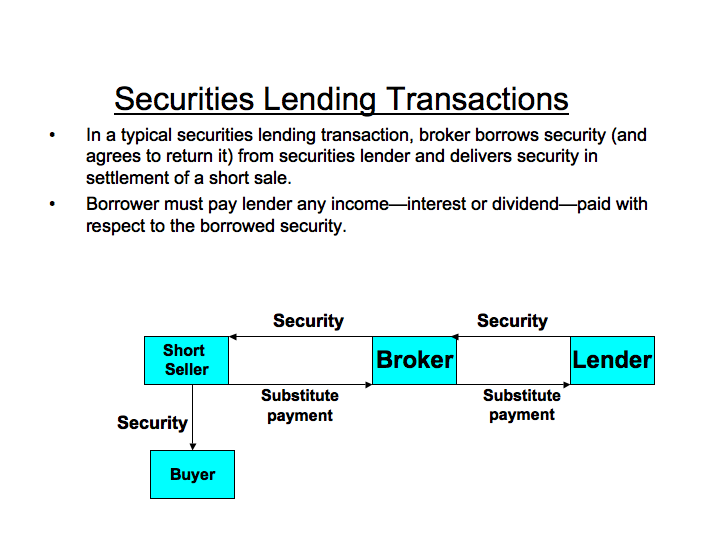
\includegraphics[width=120mm, height=70mm, clip, trim= 3mm 5mm 5mm 5mm]{seclend.png}}
\end{center}
\label{your-reference-key}
\end{figure}
Under the securities lending agreement, the borrower must pay the lender any income, such as interest or dividends, paid with respect to the borrowed security.  Under U.S. law, the substitute, or in-lieu dividend was not treated a ``dividend" for U.S. tax purposes, but rather as a fee or rent for the borrowing.  Foreign taxpayers would loan their U.S. stock over the record date and argue that the substitute dividend was not a dividend for FDAP purposes.  In addition, treaty residents argued that the income was exempt under the \emph{Other Income} article (Article 22 of the Treaty) and therefore not taxable in the source state.  

In response to these transactions, the IRS issued regulations that  adopt a look-through treatment for substitute interest and dividend payments in securities lending transactions.   Under this approach, substitute interest and dividends are sourced in the same manner as the interest or dividends accruing on the transferred security.  Reg.\@ \S\S1.861-2(a)(7) (source of substitute interest); 1.861-3(a)(6) (source of substitute dividends); 1.871-7(b)(2) (character of substitute payments); and 1.894-1(c) (treatment of substitute payments under treaties).  \margit{Substitute interest and dividend payments have the same character and source as the underlying interest or dividend.}The regulations provide that if a substitute dividend or substitute interest payment is received by a \emph{foreign person}, it has the same character as the underlying interest or dividend to which it relates for FDAP and treaty purposes. This rule has the effect of treating substitute dividends payments with respect to U.S. stock as U.S. source dividends subject to FDAP tax, but it also preserves the portfolio interest exception for substitute interest payments.

The final option employs an equity swap to avoid withholding tax.  An equity swap is a bilateral contract with a bank pursuant to which one party (for example, a bank) agrees to pay the economic appreciation with respect to a notional amount of shares of one or more companies, including both capital gain and dividends, and the other party (for example, the hedge fund) agrees to pay any depreciation with respect to the same notional amount of shares.  The party that receives the appreciation and pays depreciation is called the \emph{long party}, and the counterparty is the \emph{short party}.  The long party must also pay a financing cost that is calculated by applying an interest rate, typically LIBOR plus an additional amount, to the notional amount of the shares.  The long party thus is in the same economic position as if it had borrowed to purchase the referenced shares: it benefits by any dividend and appreciation but bears any depreciation and the financing cost of the position.

\begin{figure}[hbtp]
\caption{Equity Swap}
\begin{center}
\setlength\fboxsep{0pt}
\setlength\fboxrule{0.5pt}
\fbox{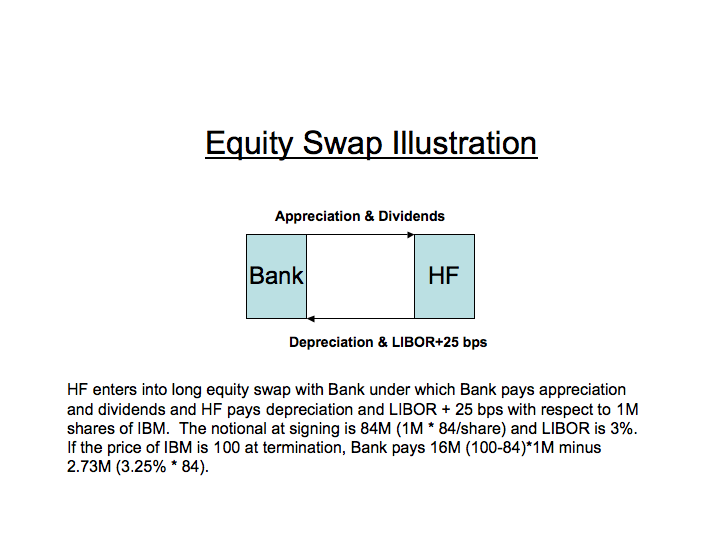
\includegraphics[width=120mm, height=80mm, clip, trim= 5mm 5mm 5mm 20mm]{equityswap.png}}
\end{center}
\label{your-reference-key}
\end{figure}

Assume that the swap payment received by a foreign hedge fund represents economically (mimics) the appreciation and dividends (less a financing charge) of a notional amount of shares of a U.S. corporation.  How should the payment be treated under section 871 or 881?  Should the gross payment be disaggregated into separate portions and the U.S. tax rules applied to each portion?  Should some portion of the swap income be U.S. source FDAP?  One issue that arises is that the payment that represents the dividend portion is generally not a dividend for U.S. tax purposes as the equity swap party does not actually own the shares and receive the payment from the dividend paying company.  Yet another issue that arises is if there is no capital gain and the financing charge offsets the notional dividend amount so that no amount is paid or received.  Also, if the swap is between two foreign parties, on what basis should the United States be able to assert tax jurisdiction over any of the payments?  Finally, would your conclusions to the questions above change if the bank had actually purchased and held the underlying shares during the term of the swap?

To encourage swap activity by U.S. banks, the IRS issued regulations in 1991 that source swap income by reference to the residence of the recipient.  Reg.\@ \S1.863-7(b)(1).  Consequently, regardless of the character of swap income, under these regulations swap income received by a foreign investor is foreign source and exempt from tax.  \margit{Swap income is generally sourced by the residence of the recipient.}That swap income representing dividends from U.S. companies was exempt from U.S. tax while the actual dividends were taxable was not lost on investment banks, who aggressively promoted swap transactions as a way for foreign hedge funds to avoid U.S. withholding tax without forgoing economic exposure to the underlying stocks.  In response to the press reports of these transactions, in 2010, Congress added new section 871(m), which provides that ``dividend equivalent payments" are treated as a U.S. source dividend for sourcing and withholding tax purposes.  A dividend equivalent payment includes substitute dividends and swap payments that are contingent upon or determined by reference to the payment of a U.S. source dividend.  


%Needless to say, the press reports of these transactions have raised concerns in Congress and the IRS.\footnote{This issue is discussed in Jeffrey M. Col\'on, \emph{Financial Products and Source Basis Taxation: U.S. International Tax Policy at the Crossroads}, 1999 University of Illinois Law Review 775 (1999)}                   

%\addcontentsline{toc}{section}{\protect\numberline{}Hedge Funds Use Swaps to Avoid Dividends} 
%\begin{select}
%\revrul{Hedge Funds Use Swaps to Avoid Dividends}{Anita Raghavan, Wall Street Journal (9/17/07)}
%
%
%Wall Street firms have long sought to use financial alchemy to save clients a bundle on their tax bills. Now, one of the Street's cleverest strategies is coming under scrutiny. 
%
%The strategy arose a few years ago, a time when lots of U.S. companies were paying fat dividends. Wall Street sensed a golden business opportunity: sell their hedge-fund clients on ways to make those dividends even fatter by avoiding taxes on them. 
%
%Bankers at Lehman Brothers Holdings Inc. pitched an enticing product. By using a complex financial tool called derivatives, hedge funds with offshore operations could reap the benefits of owning big-dividend U.S. stocks without actually owning them. The result: no dividend-tax bite. Different versions of the strategy cropped up all over Wall Street. 
%
%Hedge funds were thrilled. The Internal Revenue Service apparently wasn't. Federal tax authorities are seeking information about the trades from Lehman and Citigroup Inc., The Wall Street Journal reported in July, and other firms are bracing for similar inquiries. The government's question: Are the trades executed for any purpose other than to sidestep the dividend tax? 
%
%A look at the evolution inside Lehman of this controversial tax product shows that the firm paid considerable attention to how the IRS might react. Internal Lehman emails reviewed by the Journal reveal bankers searching for the line between smart tax planning and improper tax avoidance. In the end, according to the emails and to people familiar with Lehman's business, the bankers and their lawyers concluded that it was a business worth pursuing. 
%
%In recent years, Wall Street firms have been devising increasingly complex ways for sophisticated investors like hedge funds to minimize their tax bills. That's made it tough on tax authorities charged with deciding which maneuvers comply with tax laws and which don't. 
%
%The dividend-tax trades represent one more dimension to the spread of derivatives, complex financial instruments whose values are tied to those of assets such as stocks, commodities or currencies. Investors first turned to derivatives to hedge against risk, then as a tool to add leverage. Now, Wall Street is marketing them as a way to minimize taxes. This comes at a time when Congress is considering changing the way hedge-fund managers and private-equity firms are taxed. 
%
%The dividend-tax trades have allowed hedge funds to avoid paying more than \$1 billion a year in taxes on U.S. stock dividends, accountants and others in the business estimate. If the IRS decides the tax treatment of the trades isn't proper, it could try to slap funds with big bills for back taxes. 
%
%Nobel laureate Joseph Stiglitz, a Columbia University professor and expert witness in tax cases who examined some of the Lehman documents, says the question for tax authorities is: ``Would these trades occur at all if it were not for the tax advantages?'' If the answer is no, he says, ``at the very minimum, it is a red flag.'' 
%
%Nearly every major U.S. securities firm--from Lehman to Citigroup to Merrill Lynch \& Co.--offers such derivatives to hedge-fund clients. Foreign banks such as Germany's Deutsche Bank AG and Switzerland's UBS AG also sell the products, people familiar with the business say. 
%
%Some bankers contend that U.S. tax rules on dividends don't apply to derivatives because derivatives aren't governed by the same rules as stocks. ``We believe we are in line with industry practice as articulated by major law firms in accordance with the full knowledge of the IRS for many years,'' says John Wickham, whose job at Lehman includes overseeing the group that sells these types of derivatives. Citigroup says that the IRS views the inquiry as industrywide, and that it is cooperating. Merrill, Deutsche Bank and UBS declined to comment. 
%
%Wall Street has devised many forms of dividend-tax trades, of varying complexity. One simple kind uses a derivative called a stock swap. A Wall Street firm buys a block of stock from a hedge fund. The investment bank and the hedge fund also agree to an exchange: For a stipulated period of time, the investment bank makes payments to the hedge fund equal to the total returns on the purchased stock--the dividends plus the share appreciation--thereby simulating the benefits of actually owning the stock. In return, the hedge fund makes payments to the bank tied usually to a benchmark interest rate. If the stock declines in value, the hedge fund also must pay the bank the equivalent of the lost value. 
%
%Ordinarily, the IRS, to ensure it can collect dividend taxes from hedge funds that own U.S. stock but are domiciled outside of the country, requires securities firms to withhold the taxes from dividend payments distributed to the funds. (Domestic taxpayers are required simply to declare dividend income on their U.S. tax returns.) But when an offshore fund enters into a stock swap, who's on the hook for the dividend taxes? The U.S. banks that peddle such swaps are responsible for paying the tax, but they offset the dividend income with the expense of swap payments made to the hedge funds. The result: Because the payments received from the hedge fund are comparatively small, the bank has very little taxable income. The swap payments received by the offshore hedge fund are not subject to U.S. taxation. 
%
%The IRS declines to comment on the matter. 
%
%Hedge funds use swaps for all sorts of reasons having nothing to do with tax planning, including to lower trading costs and to make it harder for rivals to figure out what they're investing in. 
%
%The dividend-tax trading strategy became popular after changes to federal tax laws in 2003, which lowered the tax rate that individuals pay on dividends, but left the corporate rate intact. Many companies then boosted their dividend payments. European hedge funds and U.S. funds with offshore hubs jumped into these U.S. stocks, but were looking for ways to lower the tax bite. 
%
%For years, many securities firms in London, including Lehman's office there, had used derivatives to help hedge funds avoid paying a British tax known as the stamp duty, which is levied on purchases of stocks and real estate. In the summer of 2003, Richard Story, a Lehman executive in London, began pressing managers in New York to boost the volume of dividend-related derivative trades they executed, according to people familiar with the matter. 
%
%Lehman had concocted a strategy it called the Cayman Islands Trade, which offered offshore hedge funds--including the many U.S. funds with offshore operations--a way to ``enhance the yield'' on dividend-paying U.S. stocks, according to a Lehman document. The trade, which involves several legs, originates with a loan of stock from a client to a Lehman entity in the Cayman Islands. 
%
%To ascertain whether tax products will pass muster with federal tax authorities, U.S. securities firms routinely seek opinions from in-house and outside lawyers. Some legal opinions conclude that products ``will'' pass muster, while others say they ``should.'' Both grades are considered to provide acceptable legal comfort. ``More likely than not,'' a lower grade, is seen as more problematic. 
%
%``I know you got US Tax Dept (Darryl) comfortable on the Cayman yield enh. [enhancement] trades after a lot of gentle persuasion,'' Mr. Story wrote in a June 12, 2003, internal email, referring to Lehman tax attorney Darryl Steinberg. ``Did we finally get a written opinion from external counsel and if so what level of opinion was it . . . ?'' 
%
%The view from outside, at least initially, appeared fuzzy. A lawyer from Cravath, Swaine \& Moore LLP initially believed the transactions ``should'' pass muster with the IRS, according to an email to Mr. Story from Bruce Brier, a Lehman senior vice president. But after a talk with a Lehman tax lawyer, the Cravath attorney ``downgraded his opinion to `more likely than not,''' Mr. Brier wrote in the email. ``I think I can get him back to `should.'" 
%
%A Cravath spokeswoman declined to comment, as did Mr. Steinberg. Mr. Story, who no longer works at Lehman, didn't respond to requests for comment. 
%
%``You are looking at a one-page personal opinion in a thousand-page universe," a Lehman spokeswoman says. Mr. Brier's email ``in no way suggests that Cravath provided an actual written opinion and then changed it. Rather, it appears Mr. Brier and Corporate Tax were separately discussing the Cravath lawyer's possible opinion level considering a variety of different factors, some of which, when combined, would lead to a `should' level and others a `more likely than not.'" Such an exchange is ``an ordinary process of idea sharing." 
%
%Lehman touted such trades to clients in a brochure entitled ``The Power of Synthetics." The derivatives would transfer to clients ``economic exposure of a security, basket or index without taking physical ownership or delivery," the brochure said. The potential benefits included ``tax management" and ``yield enhancement," it said. 
%
%A Lehman document indicates that a number of hedge funds entered into trades, including Angelo Gordon \& Co.; Highbridge Capital Management, the big hedge fund majority-controlled by J.P. Morgan Chase \& Co.; JMG Triton; and KBC Alternative Investment Management. The Lehman document projects that the trades would save Highbridge, which has about \$37 billion in assets, about \$10.8 million in withholding taxes in 2005. JMG Triton was projected to save \$15.3 million, Angelo Gordon, \$9 million, and KBC, \$3 million, according to the document. 
%
%A KBC spokesman says, ``We have not seen that document and do not know what those numbers represent. The only reason we would track withholding taxes is if they are owed." Highbridge declined to comment. Angelo Gordon and JMG Triton didn't respond to requests for comment. 
%
%Lehman and its clients saved \$70 million in taxes they potentially owed in 2004 because of the swaps, according to the Lehman document, which refers to the withholding-tax savings as ``WHT@Risk." Lehman says the figure is from a ``draft presentation" and only represents ``one person's view of hypothetical exposure," which the firm now calls unrealistic. People familiar with Lehman's operations estimate that over the past 3 1/2; years, the firm has saved about \$200 million for its clients through such tax trades. A Lehman spokeswoman calls the figure ``conjecture." 
%
%In 2004, after Microsoft Corp. set plans to pay a one-time dividend of \$3 a share--a \$33 billion total payout--competition heated up among Wall Street firms to offer clients ways to capture a greater after-tax share of the dividend. Ian Maynard, a Lehman trading manager based in London, saw the special dividend as an opportunity for Lehman to seize business from competitors. But Lehman rivals were more aggressive, offering clients as much as 97\% of the Microsoft dividend amount compared with Lehman's 95\%, according to people familiar with the matter. 
%
%Some aspects of the business, including its profitability, worried Mr. Maynard, these people say. In a Sept. 21, 2004, email to several Lehman executives, he suggested Lehman was taking too much risk by ``guaranteeing" to pay the entire dividend amount to clients through some derivative trades. The range of clients for whom Lehman is ``guaranteeing 100\%" has ``increased significantly," he wrote. 
%
%In the email, he also noted that there appeared to be no ``consistent" standards about the minimum time clients held the derivatives, and that ``churning"--a term commonly used to refer to excessive short-term trading--appears to be ``reasonably frequent." From a tax-risk perspective, that was important. If it appeared that clients were executing such trades before dividend time, then unwinding them just after dividends were paid, tax authorities could suspect the trades were done solely to avoid taxes. 
%
%``We need to set minimum holding periods following advice from tax/compliance and eradicate any frequent churning of position," Mr. Maynard wrote. 
%
%Mr. Maynard referred questions about the matter to Lehman's spokeswoman. ``In light of evolving market conditions and technological advances," she says, ``Ian wanted to make sure that we were consistently enforcing the policies we had put in place." 
%
%Some at Lehman expressed concern over swaps tied to a single stock. Mr. Brier, the senior vice president and a tax lawyer by background, was worried the single-stock swaps could be viewed purely as a maneuver to sidestep withholding taxes, say people familiar with the situation. In an email early in 2005, he questioned whether such swaps, from a taxation standpoint, were essentially stock loans. It was a crucial question: When stocks are lent across borders, the dividend payments can be subject to taxes. 
%
%John DeRosa, Lehman's top tax official, says swaps ``possess markedly different fundamental and economic characteristics from stock loans" and thus are not subject to withholding taxes. 
%
%In a Feb. 14, 2005, email to Mr. Brier and others, Neil Sherman, a Lehman sales executive, suggested some guidelines for single-stock swaps, including that clients be required to hold them for at least 30 days. Swaps that give clients exposure to a basket of stocks could be used, he wrote, but ``care should be taken, through the observation of objective criteria, that such swaps do not have withholding tax avoidance as a principal purpose." 
%
%In a return email, Mr. Brier told Mr. Sherman it would be ``premature" to issue any new single-stock swap guidelines because, among other things, there hadn't been approval from the firm's tax department. 
%
%The Lehman spokeswoman says the directive by Mr. Sherman, who is no longer at the firm, was not triggered by any problem. Mr. Brier said recently, in a prepared statement: ``It has since come to my attention that the firm had appropriate policies in place since 2000 regarding single-equity swaps, and had previously taken legal advice from numerous outside law firms that addressed the issues which I was raising and had reached similar positive conclusions. . . . After many discussions internally and with outside counsel, it was my belief that the product was legally sound and appropriate." 
%
%At a meeting last fall of the Wall Street Tax Association, a group of tax experts, Lehman and other Wall Street firms got their first inkling that tax authorities were examining dividend-related trades, people familiar with the meeting say. Directors were buzzing about rumors of an IRS inquiry into such trades, these people say. 
%
%Todd Tuckner, UBS's tax head for the Americas, indicated that the IRS had given the bank a diagram of a transaction it appeared to be scrutinizing, the people say. After checking with the IRS, Mr. Tuckner made the diagram available to the group. Mr. Tuckner, through a spokesman, declined to comment. 
%
%Lehman still offers single-stock swaps to clients. ``Because there has been no definitive guidance to the financial community on this issue, Lehman, like its competitors, relies on its own internal analysis of the tax law and a `should'-level tax opinion from a major Wall Street law firm that clearly distinguishes our single-stock-swap trades from stock loans,'' the firm says. It declines to say which law firm provided the tax opinion. 
%\end{select}
%
%These well publicized transactions have raised concerns in Congress, which is considering changing U.S. law to treat certain swap income related to dividends on the underlying U.S. stock as U.S. source income.  

Section 871(m) is described below in an excerpt  from Joint Committee Report JCX-4-10.  The drafting of regulations implementing section 871(m) has been an arduous process because of the difficulty of finding and taxing U.S. dividend returns that are embedded in complex financial contracts, such as options and swaps.  Final regulations were issued on October 13, 2015, Reg.\@ \S1.871-15 and -15T.  These regulations were to be effective for contracts issued on or after Jan. 1, 2017.  On December 2, 2016, however, the Treasury issued Notice 2016-76, which modifies the 871(m) regulations and delays the effective date on certain complex contracts until January 1, 2018. 
 
\begin{select}
\revrul{Technical Explanation of the Revenue Provisions Contained in Senate Amendment 3310, the ``Hiring Incentives to Restore Employment Act," under Consideration by the Senate February 23, 2010.}{}

\begin{center}\textbf{Explanation of Provision}
\end{center}

The provision treats a dividend equivalent as a dividend from U.S. sources for certain purposes, including the U.S. withholding tax rules applicable to foreign persons.

A dividend equivalent is any substitute dividend made pursuant to a securities lending or a sale--repurchase transaction that (directly or indirectly) is contingent upon, or determined by reference to, the payment of a dividend from sources within the United States or any payment made under a specified notional principal contract that directly or indirectly is contingent upon, or determined by reference to, the payment of a dividend from sources within the United States. A dividend equivalent also includes any other payment that the Secretary determines is substantially similar to a payment described in the immediately preceding sentence. Under this rule, for example, the Secretary may conclude that payments under certain forward contracts or other financial contracts that reference stock of U.S. corporations are dividend equivalents.

A specified notional principal contract is any notional principal contract that has any one of the following five characteristics: (1) In connection with entering into the contract, any long party transfers the underlying security; (2) in connection with the termination of the contract, any short party transfers the underlying security to any long party; (3) the underlying security is not readily tradable on an established securities market; (4) in connection with entering into the contract, any short party to the contract posts the underlying security as collateral; or (5) the Secretary identifies the contract as a specified notional principal contract. For purposes of these characteristics, for any underlying security of any notional principal contract (1) a long party is any party to the contract that is entitled to receive any payment under the contract that is contingent upon or determined by reference to the payment of a U.S.-source dividend on the underlying security, and (2) a short party is any party to the contract that is not a long party in respect of the underlying security. An underlying security in a notional principal contract is the security with respect to which the dividend equivalent is paid. For these purposes, any index or fixed basket of securities is treated as a single security.

For payments made more than two years after the provision's date of enactment, a specified notional principal contract also includes any notional principal contract unless the Secretary determines that the contract is of a type that does not have the potential for tax avoidance.

No inference is intended as to whether the definition of specified notional principal contract, or any determination under this provision that a transaction does not have the potential for the avoidance of taxes on U.S.-source dividends, is relevant in determining whether an agency relationship exists under general tax principles or whether a foreign party to a contract should be treated as having beneficial tax ownership of the stock giving rise to U.S.-source dividends.

The payments that are treated as U.S.-source dividends under the provision are the gross amounts that are used in computing any net amounts transferred to or from the taxpayer. The example of a ``total return swap" referencing stock of a domestic corporation (an example of a notional principal contract to which the provision generally applies), illustrates the consequences of this rule. Under a typical total return swap, a foreign investor enters into an agreement with a counterparty under which amounts due to each party are based on the returns generated by a notional investment in a specified dollar amount of the stock underlying the swap. The investor agrees for a specified period to pay to the counterparty (1) an amount calculated by reference to a market interest rate (such as the London Interbank Offered Rate (``LIBOR")) on the notional amount of the underlying stock and (2) any depreciation in the value of the stock. In return, the counterparty agrees for the specified period to pay the investor (1) any dividends paid on the stock and (2) any appreciation in the value of the stock. Amounts owed by each party under this swap typically are netted so that only one party makes an actual payment. The provision treats any dividend-based amount under the swap as a payment even though any actual payment under the swap is a net amount determined in part by other amounts (for example, the interest amount and the amount of any appreciation or depreciation in value of the referenced stock). Accordingly, a counterparty to a total return swap may be obligated to withhold and remit tax on the gross amount of a dividend equivalent even though, as a result of a netting of payments due under the swap, the counterparty is not required to make an actual payment to the foreign investor.

\ldots

\end{select}

\addcontentsline{toc}{section}{\protect\numberline{}Comments}
	\begin{center}
		\textbf{\emph{Comments}}
			\end{center}



This chapter introduced the source of income rules of sections 861 and 862 for interest and dividends.  The source rules assign a source--foreign or U.S.--to items of income and expenses.  They are relevant for nonresidents because nonresidents are generally not taxed on foreign source income and for citizens and residents for purposes of the foreign tax credit rules.  The source rules do not impose any substantive tax liability, as do, for example, sections 1 and 871.  Some shady promoters and return preparers take the position that section 861 and the regulations thereunder permit a U.S. taxpayer to avoid tax on U.S. source income.  Taxpayers, even famous ones, who take such a position on a return face severe penalties and possibly imprisonment.  See Rev. Rul.  2004--30, 2004--1 C.B. 622.    
%\addcontentsline{toc}{section}{\protect\numberline{}Snipes Indicted for Tax Evasion} 
\begin{select}
	\revrul{Snipes' Sentence a Big Win for Tax Officials} 

Action star Wesley Snipes' three-year sentence on tax charges is a big win for prosecutors.

As Forbes reported earlier this week,\footnote{\url{http://bit.ly/2jyPamb}. A copy of the Snipes's amended 1997 tax return can be found at \url{http://bit.ly/2k4gnhr}} officials are increasingly concerned about a growing number of so-called ``tax defiers." Prosecutors pushed hard for a tough sentence in the Snipes case, worrying that anything less risked emboldening the movement.

Tax defiers--or ``tax protesters" as they've traditionally been known--glom onto one kooky, discredited theory or another as to why the income tax is illegal or doesn't apply to them personally or doesn't cover their normal sources of income. (Example: Only foreign income, or only earnings of federal employees are taxable.) They typically file returns showing zero income or simply stop filing. Sometimes they also put in claims for refunds on taxes they paid before their conversions, as Snipes did. 

Snipes was the highest-profile criminal tax target in years, and prosecutors called for a heavy sentence to deter others from trying to impede the IRS. The government alleged Snipes earned at least \$13.8 million in income for the years in question, on which he owed \$2.7 million in back taxes. 

Snipes was acquitted in February of five additional charges, including felony tax fraud and conspiracy. Snipes' co-defendants, Douglas P. Rosile and Eddie Ray Kahn, were convicted on both those counts. Kahn, who refused to defend himself in court, was sentenced to 10 years, while Rosile received 54 months. Both will serve three years of supervised release. Snipes will serve one year of supervised release. 

In court Thursday, Snipes read from a statement, apologizing for his ``costly mistakes," but never mentioned the word ``taxes." 
\end{select}

\addcontentsline{toc}{section}{\protect\numberline{}Interest and Dividend Problems} 
	\begin{center}
		\textbf{Interest and Dividend Problems}
	\end{center}
	\begin{select}
 	\textit{First determine the source of the item of income (sections 861-865), the taxation of the item (section 871 or 881), and finally whether the payor of the item must withhold (section 1441 or 1442).  Answer each of the problems below first assuming that the recipient is not entitled to the benefits of any income tax treaty, and then determine whether your answer would be modified by the Treaty.  Dividends and interest are addressed in Articles 10 and 11.}   
 	\begin{enumerate}
		\item Interest paid to a U.K. citizen and resident:
			\begin{enumerate} 
				\item on a corporate bond issued by Coca Cola.  The bond holder doesn't own any stock. [1441(c)(9); Reg.\@ \S 1.1441-1(b)(4)(i); and the ConAgra Foods prospectus]
				\item on a CD issued by the New York branch of Citigroup Inc., a U.S. corporation.[871(i)(2)(A); 1441(c)(10); Reg.\@ \S 1.1441-1(b)(4)(ii), -(e)(3)]
				\item on a CD issued by a U.K. branch of Citigroup. [Reg.\@ \S 1.1441-1(b)(4)(iii)]
				\item on a tax-exempt NYC municipal bond [Reg.\@\@ \S 1.861-2(a)(1)] (Regardless of the source of interest, why shouldn't foreigners generally buy U.S. tax-exempt bonds?)
				\item For each of the above questions, very briefly describe what documentation, \emph{if any}, the U.K. resident should provide to the U.S. payor.  
			\end{enumerate}
		\item A U.K. resident holds a bond of DC, a Delaware corporation, that pays annual interest of \$100.   Assume alternatively:
			\begin{enumerate}
				
				\item The bondholder owns 15\% of DC's voting stock.
				
%				\item The bondholder owns 15\% of DC's voting stock, and the first interest payment of \$100 is made during DC's first taxable year.  DC's gross income for this year consists of \$750 from a construction project in Brazil and \$250 as interest on deposits with banks in the U.S. [861(c)(1)]
%				\item The bondholder owns 15\% of DC's voting stock and DC's gross income consists of \$850 from a construction project in Brazil and \$150 as interest on deposits with banks in the U.S. [861(c)(1), (c)(2)(B)]
				\item Same as previous question, except that the U.K. resident owns 5\% of DC's stock.
				\item Same as previous question, except that the bond was guaranteed by DC's parent, a Cayman corporation.  DC defaults on an interest payment, and the Cayman corporation pays as guarantor. [Reg.\@\@ \S 1.861-2(a)(5)]
			\end{enumerate}  		
			
			\item A U.K. bank loans money to a U.K. branch of IBM, which pays interest on the loan to bank. [\S 881(a), (c)]
			
			\item A U.K. parent corporation loans money to its wholly owned U.S. subsidiary, which pays interest to the parent.
			
			\item UKPS, a U.K. partnership, owns 50\% of the stock and 20\% of the debt of USCo, a U.S. corporation.  UKPS has 100 equal partners.  USCo makes an interest payment to UKPS. [Reg.\@ \S 1.871-14(g)]
			
			\item PS, a partnership organized under U.S. law, borrows money from a Brazilian citizen.  PS carries on a trade or business in the U.S., but this business produces only a small portion of PS's income (5\%), and the borrowing has nothing to do with the U.S. business.  The Brazilian owns 15\% of PS. Note, partnerships compute their income in the same way as individuals (\S 703).  [861(a)(1), (a)(1)(B); Reg.\@ \S1.861-2(a)(2)] 
			
			\item  PS, a partnership organized under U.S. law, has only U.S. partners, and invests in start-up companies.  (Under U.S. law, such a partnership would probably \emph{not} be considered to have a U.S. trade or business.)  It borrows money from Citigroup. What is the source of the interest paid?  [Reg.\@ \S 1.861-2(a)(2)]
			
			\item U.K. resident receives a dividend from IBM.
			
			\item U.K. resident purchases debt issued by IBM that promises a fixed interest rate of 6\% per annum plus 1\% of IBM's preceding year's cash flow.  U.K. resident receives an interest payment of \$80, of which \$60 is attributable to the fixed interest rate and \$20 to the cash flow. [871(h)(4)]
			
			\item U.K. parent corporation receives a dividend from its wholly owned U.S. subsidiary.
			
			\item A U.K. pension fund receives a dividend from IBM. 
			
			\item USP, a partnership formed in the U.S. that is not engaged in a U.S. trade or business, receives a dividend from IBM.  Paul, a U.K. resident is a 10\% partner in USP.  [Reg.\@ \S 1.1441-5(b)(1), (2)(i)(A); Article 1(8)]
			
			\item UK Ltd. is a UK entity treated as a corporation for U.K. purposes but as a partnership for U.S. purposes.  This is a hybrid entity.  Paul, a U.K. resident owns 10\% of UK Ltd.  UK Ltd. receives a dividend from IBM.   [Reg.\@ \S 1.1441-5(c)(1)(i), (ii), and (iii); Article 1(8)] 
			
			\item USP, a U.S. citizen residing in London, owes money to U.K. bank and has given an interest bearing note to evidence the obligation to repay.  Now, assume that USP moves back to the U.S. and continues to pay interest on the note.  [Reg.\@ \S 301.7701(b)-1(a).]
			
%			\item UKP, a citizen and resident of the U.K., is a shareholder in FC, a U.K. corporation.  FC has gross income of \$600 each year during years 1 through 3 from a business carried on in the U.S. and had gross income for this period from foreign operations of \$400 annually.  Its taxable income effectively connected with its domestic business was \$60 per year, and foreign business profits were \$100 per year.  Late in year 3, FC received a dividend of \$600 from a foreign subsidiary that derives all of its income from businesses carried on outside the United States.  FC then distributed the \$600 to its shareholders a few weeks later in year 3.  How would your answer change if the distribution occurred in year 4? [861(a)(2)(B); 871(i)(2)(D)]
			
			\item UKP, a U.K. citizen and resident, owns a share of IBM.  UKP loans the stock to B, a U.S. broker/dealer, under a securities lending transaction, who sells it to C, a U.S. institutional investor.  B posts with UKP the sales proceeds as cash collateral.  This amount is adjusted daily to reflect changes in the value of the IBM stock.  Thus, if IBM rises, B pays UKP, and vice versa.  UKP pays interest on the cash collateral equal to the market rate less 50 basis points.  A dividend of \$100 per share is paid by IBM on the stock, and, pursuant to the lending agreement, \$100 is remitted to UKP as a substitute dividend payment.  What are the U.S. tax consequences to UKP?  [\S871(m); Reg.\@ \S1.894-1(c); and Article 22.]	
			
				\item Same initial facts as previous question, except that UKP sells the stock directly to C and enters into an equity swap with B, under which B pays to UKP any increase in the value of IBM stock (daily, quarterly, or yearly) and any dividends paid during the period of the swap, and UKP pays to B an amount reflecting the market rate of interest on a notional principal amount equal to the value (measured daily, quarterly or yearly) of the IBM stock, and any decrease in the value of the stock.  A \$100 dividend is paid by IBM and B pays UKP \$100 less \$5 of financing costs.  (It would be a very fruitful exercise to compare the economic returns UKP would earn if the stock went up or down by \$100 assuming that (1) he actually owned it;  (2) he was a party to the above swap contract; (3) or he loaned out the stock in a securities lending transaction.)  Assume the current price is \$300 per share.  What are the U.S. tax consequences to UKP? [\S871(m); Reg.\@ \S1.894-1; and Article 22.]
 \end{enumerate}
 	\end{select}

\begin{framed}
	\center{Last revised Aug. 23, 2015; source\_IntDiv\_Jan17\_17}
	\end{framed}
		 \section{Compensation for Services}
\crt{861(a)(3); 863(b)(1); 864(b)(1); 864(c)(6); 871(a)(1); 881(a)(1); 1441(b)(1) and (c)(1); and 1442(b)(2)}{1.861-4(b)(1), (2)(i), (2)(i)(A), (2)(E), and (F); 1.864-4(c)(6); Prop. 1.861-4(b)(2)(ii)(G); 1.1441-1(a) and (b); and 1.441-2(b)(2)(i)}{Articles 7, 14, 15, 16, 17-19 (skim lightly), and 20}

Compensation for services performed in the United States is generally U.S. source income.  \S861(a)(3).  If services are performed solely in the United States or abroad, determining the source of compensation for those services is straightforward.  There is a \emph{de minimis} exception for compensation not exceeding \$3,000 performed by a nonresident alien who is present for 90 days or less in the United States and works for either a foreign person not engaged in a U.S. trade or business or for a U.S. person if the services are performed in connection with the U.S. person's foreign place of business.  \S\S 861(a)(3)(A)-(C); 864(b)(1)(A)-(B).  As the \$3,000 limit \margit{\$3,000 in 1936 is equivalent to \$51,418 in 2016.}has not been adjusted for inflation since the provision was enacted over 60 years ago, the rule probably affects very few persons.  

If a person receives compensation for performing services both in the United States and abroad, the compensation must be allocated between U.S. and foreign sources. \S863(b)(1).  Since an employee who performs services inside and outside of the United States will often not receive separate compensation for the U.S. and foreign services, is it necessary to allocate the income between U.S. and foreign sources by examining the employee's employment contract or another method.  Regulations under section 861 provide that the allocation is to be made ``on the basis that most correctly reflects the proper source of that income under the facts and circumstances of the particular case.  In many cases, the facts and circumstances will be such that an apportionment on a time basis\ldots will be acceptable.''  Reg.\@ \S1.861-4(b)(2)(i).  The same regulation also provides rules for sourcing certain benefits, such as housing, education, local transportation, tax reimbursements, hazardous pay, and moving expenses.    Reg.\@ \S1.861-4(b)(2)(ii)(D)(1)--(6).

The \emph{Stemkowski} case below illustrates how this determination is made in the absence of a specific allocation in an employment contract.  Compensation received by athletes and artists presents particular challenges.  The event(s) for which an athlete or artist is ultimately compensated may represent the culmination of much preparation, rehearsals, and training performed in locations different than the final performance(s).  Some had argued that an athlete or artist could allocate compensation between the countries where he performed and trained or rehearsed.  In 2007, the IRS issued proposed regulations under section 861 that provide that compensation received for performing services at a specific event should be allocated entirely to where the event occurs.  The preamble to the proposed regulations states that it is probably improper to allocate any of the compensation for services received to the place where the artist or athlete prepares for the performance.  \emph{See} Prop. Reg.\@ 1.861-4(b)(2)(ii)(G), (4)(c), Ex. 10 (player contract compensation not allocated to preseason or postseason unless athlete receives additional compensation).  The proposed regulations thus would overturn the portion of \emph{Stemkowski} that allocated a portion of the contract income to the preseason and postseason.  

Although compensation is listed as FDAP under section 871(a), if U.S. source compensation is received in a year in which the service provider is engaged in a U.S. trade or business, it will not be taxed at a flat 30\%, but instead is taxed as effectively connected income at graduated rates.  Performing services in the United States for even one day constitutes a U.S. trade or business, thereby subjecting the U.S. source income to graduated rates.  \S 864(b); Reg.\@ \S 1.864-4(c)(6). There is a narrow exception in \S 861(b)(1)(A) that parallels the exception in \S861(a)(3) for minor amounts of compensation paid to nonresidents temporarily present in the United States.  

Prior to 1986, deferred compensation paid in a year in which a nonresident was not engaged in a U.S. trade or business could be subject to tax under section 871 if it were U.S. source.  If the recipient resided in a treaty country, however, the deferred compensation may have escaped U.S. tax entirely.  To prevent this gambit, Congress, in 1986, enacted section 864(c)(6), which treats deferred compensation of a nonresident received in a year in which he is not engaged in a trade or business, but which is attributable to services performed in the U.S. in another year, as if it had been received in the other year.  Thus, only in very rare circumstances will compensation be taxed as FDAP.    

Treaties take a much more nuanced approach to compensation than the Code.  Compensation performed as an independent contractor, \emph{e.g.}, an attorney, accountant, or engineer, is governed by Article 7.  Compensation for services rendered as an employee working for an employer of the other treaty country is not subject to source basis taxation, provided the employee is present in the source country for not more than 183 days.  Article 14.  On the other hand, directors's fees for services performed for a company resident in one country can be taxed by the source country, regardless how many days the director is present in the source country.  Article 15.  Separate articles apply to income of sportsmen and entertainers, income from pensions, income from government services, and income of students and teachers.  \emph{See} Articles 16-20.    

\addcontentsline{toc}{section}{\protect\numberline{}Stemkowski v.\@ CIR} 
\begin{select}
\caseart{Stemkowski v.\@ CIR}{ 690 F.2d 40 (2nd. Cir. 1982)}{Oakes, Circuit Judge}
\ldots
\begin{center} \textbf{FACTS}
\end{center} 
Taxpayer was traded prior to the beginning of taxable year 1971 to the New York Rangers, who play their home games at Madison Square Garden in New York City. He had previously signed a two-year NHL Standard Player's Contract with the Detroit Red Wings, and this contract was assigned to and assumed by the Rangers. The contract provided for compensation of \$31,500 in the 1970-71 season and \$35,000 in the 1971-72 season plus various NHL bonuses, including a \$1500 bonus for each round won in the play-offs. The player agreed to give his services in all ``league championship'' (i.e., regular season), exhibition, and play-off games, to report in good physical condition to the club training camp at the time and place fixed by the club, to keep himself in good physical condition at all times during the season, and to participate in any and all promotional activities of the club and the league that in the opinion of the club promoted the welfare of the club or professional hockey.

In addition to their rights under this contract, NHL players in 1971 were entitled under the NHL's Owner-Player Council Minutes and Agreements to receive \$25 per exhibition game plus \$25 per week of training camp unless they had played fifty or more games in the previous season, in which case they received \$600 in lieu of payments for exhibition games and training camp allowances other than transportation, food, and lodging. The players were also provided with medical and disability coverage, per diem expenses while traveling during the regular season, and various other benefits.

An NHL player's year is divided into four periods: (1) training camp, including exhibition games, beginning in September and lasting approximately thirty days; (2) the ``league championship'' or regular season of games beginning in October and lasting until April of the following year; (3) the play-off competition, which ends in May; and (4) the off-season, which runs from the end of the regular season for clubs that do not make the play-offs, or from a club's last play-off game, to the first day of training camp. Stemkowski lived in Canada during all of the off-season and most of the training camp period and played in Canada fifteen days out of 179 during the regular season and five out of twenty-eight days during the play-offs. When he was not living in Canada or travelling to games elsewhere, he lived in Long Beach, New York, near New York City, where he shared a rented house with other professional hockey players.

On his tax return, Stemkowski reported \$44,271 in income, of which he initially excluded \$10,625 as earned in Canada\ldots

The less time Stemkowski was in the United States during the period covered by his contract, the less United States tax he owes. Thus, Stemkowski could reduce his tax liability either by showing that he was in Canada for a longer period during the time covered by the contract or, as is at issue here, that the contract covered a time during which he was in Canada. The Tax Court held that the total number of days for which Stemkowski was compensated under his contract was not 234 (all but the off-season) as he had claimed on his tax return, or 365 as he had claimed before the Tax Court, but only 179, the number of days in the regular season. The Tax Court held that Stemkowski could not use days spent in Canada during training camp, the play-offs, or the off-season in calculating his foreign-source exclusion from income. The Tax Court further found that Stemkowski's off-season physical conditioning expenses, because incurred solely in connection with his contractual obligation to show up in good condition at training camp in Canada, were not connected to income from the conduct of a trade or business within the United States and thus were not deductible. \ldots

\begin{center} \textbf{DISCUSSION}\\
\textbf{1.  Allocation of Income}
\end{center} 
The first issue is the Tax Court's determination of the portion of Stemkowski's compensation under the NHL Standard Player's Contract that was drawn from United States sources. As a nonresident alien, Stemkowski was taxable on income connected with the conduct of a trade or business, including the performance of personal services, within the United States. I.R.C. \S\S 871(b), 864(b). Where services are performed partly within and partly outside the United States, but compensation is not separately allocated, Treas. Reg.\@ \S 1.861-4(b) (1975) allocates income to United States sources on a ``time basis'':
\begin{quote} 
(T)he amount to be included in gross income will be that amount which bears the same relation to the total compensation as the number of days of performance of the labor or services within the United States bears to the total number of days of performance of labor or services for which the payment is made.
\end{quote} 
This regulation applies to Stemkowski because the NHL Standard Player's Contract does not distinguish between payments for services performed within and outside the United States.

The parties disagree on what components of a hockey player's year are covered by the basic compensation in the NHL Standard Player's Contract, and therefore on how to compute the time-basis ratio. The taxpayer contends here as he did before the Tax Court that the contract salary compensates him for training camp, play-off, and even off-season services. The Commissioner argues and the Tax Court held that the contract salary covers only the regular season, and therefore that contract salary should be allocated to United States income in the same proportion that the number of days played in the United States during the regular season (164) bears to the total number of days in the regular season (179).\footnote[4]{Although the Tax Court did not discuss separately the component of Stemkowski's total reported income representing play-off bonuses, the Commissioner concedes that Stemkowski's play-off compensation should be allocated separately from his contract salary, according to a ratio whose numerator contains the number of Ranger play-off days in the United States (23), and whose denominator contains the total number of Ranger play-off days in 1971 (28).} We agree with the Commissioner and the Tax Court that the contract does not cover off-season services, but we hold that the Tax Court's finding that the contract does not compensate for training camp and the play-offs as well as the regular season is clearly erroneous. 

The Tax Court's holding was premised on provisions in the NHL contract and other players' agreements, and on the testimony of league and club officials. The first paragraph of the NHL Standard Player's Contract provides that if a player is ``not in the employ of the Club for the whole period of the Club's games in the National Hockey League Championship Schedule,'' i.e., for the entire regular season, then he receives only part of his salary, in the same ratio to his total salary as the ``ratio of the number of days of actual employment to the number of days of the League Championship Schedule of games.'' Paragraph 15 provides that if a player is suspended, he will not receive that portion of his salary equal to the ratio of ``the number of days (of) suspension'' to the ``total number of days of the League Championship Schedule of games.'' The Tax Court concluded from these two paragraphs, and from the NHL's further agreements to pay players separate bonuses for participating in the play-offs and flat fees plus travel, room, and board for participating in training camp and pre-season exhibition games, that the basic contract salary did not cover play-off or training camp services. \ldots

We cannot uphold that finding, as we believe it clearly erroneous. The formulas for docking salary given in the contract's first and fifteenth paragraphs are not persuasive evidence that the salary compensates only for the regular season. These formulas may well use the number of days in the regular season in their denominators for administrative convenience (e.g., because the number of days to be spent in the play-offs cannot be known in advance) or to maximize the salary penalty per day lost. As to the testimony relied upon by the Tax Court, to a certain extent the owners and league officials have an interest in having the contract cover the shortest possible timespan so as to maximize loss to suspended or striking players. Furthermore, two of the league and club officials, Leader and McFarland, testified that at least training camp time was included in the contract. The contract's plain language, moreover, requires in Paragraph 2(a) that a player ``report to the Club training camp ... in good physical condition,'' and a player who fails to report to training camp and participate in exhibition games is subject under Paragraph 3 to a \$500 fine, deductible from his basic salary. True, experienced players were paid \$600 plus room and board for training camp under the Owner-Player Council minutes and Agreements, but we read those Agreements as providing that amount merely to cover the additional expenses of being away from home at training camp.

Paragraph 2 of the contract also plainly requires a player's participation in play-off games in exchange for basic contract salary. While it is true that bonuses are provided for play-off games won, these are simply added incentives, above and beyond salary, to get into and win the play-offs. In this respect, they are just like other incentive bonuses the contract provides to influence conduct during even the regular season,\emph{e.g.}, bonuses for the club's finishing in third place or better (\$2500 in this case), or for the number of goals a player scores per season above certain minimums (at least \$100 per goal over 20). Furthermore, players are required to participate in all play-off games for which they are eligible. Players may be terminated for failure to participate in the play-offs, but players receive nothing for the play-off games that they lose. Thus, we hold that the basic contract salary covered both play-off and training camp services.

We agree, however, that the off-season is not covered by the contract. During the off-season, the contract imposes no specific obligations on a player. Stemkowski argues that the obligation to appear at training camp ``in good condition'' makes off-season conditioning a contractual obligation. Fitness is not a service performed in fulfillment of the contract but a condition of employment. There was no evidence that Stemkowski was required to follow any mandatory conditioning program or was under any club supervision during the off-season. He was required to observe, if anything, only general obligations, applicable as well throughout the year, to conduct himself with loyalty to the club and the league and to participate only in approved promotional activities. 

\ldots
\end{select}


%  \addcontentsline{toc}{section}{\protect\numberline{}Excerpt from the Proposed Regulations on the Source of Compensation of Athletes and Artists} 
%\begin{select}
%\revrul{Excerpt from the Proposed Regulations on the Source of Compensation of Athletes and Artists Regulations (Prop. Reg.\@ \S 1.861-4(b)(2)(ii)(G)(g))}{October 11, 2007}       
%
%\begin{center}\emph{Explanation of Provisions}
%\end{center}
%
%\ldots
%
%The amount of income received by a person, including an individual who is an artist or an athlete, that is properly treated as compensation from the performance of labor or personal services is determined based on all of the facts and circumstances of the particular case. Proposed section 1.861-4(b)(2)(ii)(G) specifies that the amount of compensation for labor or personal services determined on an event basis is the amount of the person's compensation which, based on the facts and circumstances, is attributable to the labor or personal services performed at the location of a specific event.
%
%The IRS and the Treasury Department have determined that the proper source of compensation received by a person, including an individual who is an artist or athlete, specifically for performing labor or personal services at an event is the location of the event. A basis that purports to determine the source of compensation from the performance of labor or personal services at a specific event, whether on a time basis or otherwise, by taking into account the location of labor or personal services performed in preparation for the performance of labor or personal services at the specific event will generally not be the basis that most correctly determines the source of the compensation. This rule applies to situations covered by section 1.861-4(a) and (b).
%
%Under section 1.861-4(a), the source of compensation for labor or personal services performed wholly within the United States is generally from sources within the United States. Therefore, if a person, including an individual who is an artist or an athlete, is specifically compensated for performing labor or personal services at an event in the United States, the source of such compensation is wholly within the United States because the labor or personal services were performed wholly at an event within the United States. The proposed regulations state that a basis that purports to determine the source of such income on a time basis by taking into account the location of labor or personal services performed in preparation for the performance of labor or personal services at the specific event will generally not be a more reasonable basis for determining source of the compensation. The proposed regulations add an example to section 1.861-4(c) to illustrate the application of this rule.
%
%Section 1.861-4(b) applies to instances in which a person is compensated for performing labor or personal services at multiple events, only some of which are within the United States, and at least a portion of the person's compensation cannot be specifically attributed to the person's performance of labor or personal services at a specific location. If the person is not an individual who is compensated as an employee, the source of compensation for labor or personal services is determined on the basis that most correctly reflects the proper source of that income under the facts and circumstances of the particular case. See section 1.861-4(b)(1) and (2)(i). If a person is compensated specifically for labor or personal services performed at multiple events, the basis that most correctly reflects the proper source of that income under the facts and circumstances of the particular case will generally be the location of the events. In addition, a basis that purports to determine the source of such income on a time basis by taking into account the location of labor or personal services performed in preparation for the performance of labor or personal services at the specific event will generally not be the basis that most correctly reflects the proper source of the compensation under proposed section 1.861-4(b)(2)(ii)(G).
%
%The Commissioner may, under the facts and circumstances of the particular case, determine the source of compensation that is received by an individual as an employee under an alternative basis if such compensation is not for a specific time period, provided that the Commissioner's alternative basis determines the source of compensation in a more reasonable manner than the basis used by the individual. Compensation specifically for labor or personal services performed at a specific event is not compensation for a specific time period. The basis that most correctly reflects the proper source of that income will generally be the location of the event under proposed section 1.861-4(b)(2)(ii)(G). In addition, a basis that purports to determine the source of such income on a facts and circumstances basis by taking into account the location of labor or personal services performed in preparation for the performance of labor or personal services at the specific event will generally not more properly determine the source of the compensation under proposed section 1.861-4(b)(2)(ii)(G).
%
%\end{select}

The source of income received for \emph{not} performing services, for example as pursuant to a non-compete contract, is addressed in \emph{The Korfund Company, Inc.\@ v.\@ CIR}.  The \emph{Korfund} court concludes that payments to a nonresident for agreeing \emph{not} to compete in the United States are U.S. source because had the nonresident violated the contract not to compete, the place of performance would have been the United States.  Is this conclusion sound, especially today?  Would the nonresident have had to have been present in the United States to violate the non-compete agreement?  Also, why is the IRS going after Korfund instead of the nonresidents?  Can U.S. persons use the holding in \emph{Korfund} to generate untaxed foreign source income?

\addcontentsline{toc}{section}{\protect\numberline{}The Korfund Company, Inc. v.\@ CIR} 
\begin{select}
\caseart{The Korfund Company, Inc. v.\@ CIR}{ 1 T.C. 1180 (1943)}{Disney, Judge}
\ldots
\begin{center} \textbf{FINDINGS OF FACT}
\end{center}
[Korfund] is a New York corporation organized in 1924, \ldots [and it manufactures and sells] foundation material, such as cork plates and vibration absorbers. [The shareholders at formation were] Hugo Stoessel, a nonresident alien and citizen of Germany [925 shares] and Siegfried Rosenzweig [75 shares] \ldots

The Emil Zorn Aktiengesellschaft [Zorn] is a nonresident foreign corporation engaged in the same business as petitioner, with its principal office in Berlin, Germany. In 1928 its stock was held equally by Stoessel and Werner Genest, a nonresident alien and citizen of Germany. In 1932 or 1933 Stoessel became the sole owner of stock of Zorn.

On October 22, 1926, petitioner entered into a written contract in the United States with Zorn whereby Zorn agreed (a) not to compete with petitioner in this country and Canada or to form, or give any data for the purpose of forming, a competitive company in that territory until the end of 1945, and (b) to give technical and business advice to petitioner upon its request, and petitioner agreed (a) not to furnish material, for the isolation of noise and vibration, outside of the United States and Canada prior to December 31, 1945, except specified territory outside of European countries. Each party agreed to turn over inquiries received from territory of the other and to exchange without charge improvements, inventions, and patents involving isolation against noise and vibration. Zorn was to receive from petitioner quarterly ``a royalty of 1 1/2\% for the year 1926 and 2\% thereafter of the sale of all cork plates with iron frames and of 4\% of the sale of all vibration absorbers,'' computed in a specified manner, with a minimum payment of \$400 for 1926, \$1,000 for 1927, and \$1,250 thereafter through 1940. Zorn did not own any patents at that time. One of the purposes of the contract was to eliminate competition.

On September 21, 1928, the stock of petitioner was held as follows: Stoessel and Genest each 250 shares, Herman Hoevel 299 shares, and Siegfried Rosenzweig 201 shares. \dots

\ldots

On September 21, 1928, petitioner entered into a written agreement with Stoessel in the United States whereby Stoessel undertook to act as consultant and adviser of petitioner in matters relating to the business of petitioner and to communicate to it information of value to petitioner's business until December 31, 1939, for 10 percent of the net earnings of petitioner payable at the end of each year. He also agreed not to act in a similar capacity for any other person, association, or corporation in the United States engaged in the same or a similar business. One of the purposes of the agreement was to eliminate competition.

\ldots

Zorn and Stoessel faithfully performed their agreements not to compete with petitioner and not to give advice to its competitors. On about January 1, 1933, petitioner canceled the contracts of September 21, 1928, and October 22, 1926, with Stoessel and Zorn, and refused to make further payments to them. The contract with Stoessel was canceled on account of his failure to communicate technical information relating to petitioner's business as required by the agreement.

\ldots

On July 30, 1934, Zorn assigned to Bernard Voges, New York City, all sums due it from petitioner under the agreement of October 22, 1926, and Stoessel assigned to the same individual salary in the amount of \$1,984.04 alleged to be payable by petitioner for services rendered prior to October 1, 1932, and the balance of \$2,227.60 payable to him from surplus account, plus interest on the claims of each, with power to recover the amount, plus interest on the claims of each, with power to recover the amounts for the account of the assignors. Voges instituted suit against petitioner in August 1934 under the assignments. An understanding was reached in 1934 to settle the claims by a payment of \$2,750 to Stoessel and \$3,250 to Zorn. The claim of Zorn for \$3,250 and the claim of Stoessel for \$2,227.60 were allowed in full. The remaining amount allowed Stoessel was for demands made under the agreement of September 21, 1928. The total amount was placed at interest and earned interest of \$80, pending approval of the settlement by the German Government. Final settlement was made in 1938 when \$2,508 was paid to Stoessel and \$2,964 to Zorn and \$608 was withheld for payment of withholding taxes.

\begin{center} \textbf{OPINION}
\end{center}

In his determination of the deficiency the respondent held that the allowance of \$2,786.67 to Stoessel and \$3,293.33 to Zorn, which amounts include the proportionate share of each in the interest of \$80, constituted income from sources within the United States on which petitioner, as withholding agent, should have paid a tax equal to 10 percent of the former amount and 15 percent of the latter amount in accordance with the provisions of sections 143 and 144 of the Revenue Act of 1938. The item of \$2,786.67 includes the principal sum of \$2,227.60 representing Stoessel's share of petitioner's old surplus of \$24,910.40. Respondent admits that, of the total amount paid to Stoessel in 1938, \$2,227.60 represented the dividend and the remainder compensation under the contract. The parties differ only on whether this item of \$2,227.60 was received by Stoessel in the taxable year. \ldots

\ldots

Under their contracts Zorn and Stoessel agreed, in general, to act as consultants to petitioner. In addition Zorn agreed not to compete with petitioner or give any information for the formation of a competitive company and Stoessel agreed not to act as consultant to a competitor of petitioner. All of the amount paid to Zorn and the amount paid to Stoessel in excess of the surplus item were paid for these two general classifications of undertakings without any segregation of the amount paid for each. The respondent subjected the entire amounts to withholding tax, presumably in the absence of any basis of segregation, for he does not contend that the income from services performed as consultants is subject to the tax. Not only was no evidence offered on which to make an apportionment, but petitioner does not, upon brief, suggest or request an allocation. Under the circumstances, no apportionment is possible and we will regard all of the amounts in question under this point as having been earned by the nonresident aliens for obligations under the contracts other than service as consultants. See Estate of Alexander Marton, 47 B.T.A. 184.

The sole point of difference between the parties as to this income is whether it was earned from sources within the United States within the meaning of section 119 of the Revenue Act of 1938, and that, as already indicated, turns upon the source of the income derived from agreements not to compete with petitioner in the United States and Canada or give advice for the organization of, or to, a competitor.

The petitioner's contention is based upon the theory that the income was paid for agreements to refrain from doing specific things--negative acts. No defaults occurred and during the period of compliance the promisors were residents of Germany. Petitioner's contention is that negative performance is based upon a continuous exercise of will, which has its source at the place of location of the individual, and that, as the mental exertion involved herein occurred in Germany, the source of the income was in that country, not in the United States where the promise was given. The respondent's view of the question is, in short, that, as the place of performance would be in the United States if Zorn and Stoessel had violated their contractual obligations, abstinence of performance occurs in the same place. Petitioner relies upon Piedras Negras Broadcasting Co., 43 B.T.A. 297; affd., 127 Fed.(2d) 260.

In the Piedras Negras Broadcasting Co. case the taxpayer, a Mexican corporation, owned and operated a radio broadcasting station in Mexico, from which it broadcast programs primarily for listeners in the United States, for which it received compensation in the United States from citizens thereof. In holding that the source of such income was not within the United States, we pointed out that the studio and broadcasting plant were located, and operated by the employment of capital and labor, in Mexico; that the source of the income was, accordingly, in such studio and power plant, and that the reception of the radio impulses in receiving sets in this country was secondary, not the primary source. The court in affirming the decision said that ``the source of income is the situs of the income-producing service'' and that the source of the income was ``the act of transmission.'' This reasoning is said to be equally applicable to the situation here.

In Sabatini v.\@ Commissioner, 98 Fed.(2d) 753, the taxpayer was an author and a subject of Great Britain. He was not in the United States before, nor during, the taxable years. By contract executed outside the United States he gave to a publisher in this country, among other rights, the right to publish certain books, as to some of which copyrights were not obtainable. As to these the taxpayer, by the contract above mentioned, agreed not to authorize any other publisher to publish the books in the United States so long as the publisher left in print its editions of the books. The taxpayer was to receive under the contracts amounts determinable from the number of volumes sold. In holding that the income paid based upon the sale of these books was derived by the taxpayer from sources within the United States, the court said:
\begin{quote}The payments were received in consideration of his granting the publisher the exclusive right to publish here. To be sure, that may not have been of great value but the parties did value it and the author received the payments as agreed. We are not now concerned with the quality of the consideration he gave but only with the taxability of that which he received. The payments were made to him for foregoing his right to authorize others for a time to publish the works here. Though others may, perhaps, lawfully have published them they could not do so under his express authority. The rights he granted were an interest in property in the United States, in the one instance the statutory copyrights obtainable and in the other the exclusive right to publish with his permission.
\end{quote}

In Ingram v.\@ Bowers, 47 Fed.(2d) 925; affd., 57 Fed.(2d) 65, Enrico Caruso, a nonresident alien, entered into a contract in the United Stated to sing for the Victor Talking Machine Co. for the purpose of making phonograph records of selections rendered by him. The agreement contained a provision that Caruso would not permit any records of his voice to be made by any other concern. He was to receive under the contract a specified amount of the selling price of records sold, with a minimum yearly payment. In holding that the income received by Caruso under the contract from foreign sales constituted income from sources within the United States, the court pointed out that the decisive feature was the fact that the services were rendered in the United States and that those services were the source of all income derived from the contracts. No point appears to have been made of the fact that some part of the income was paid for the promise to refrain from singing for others, as it is not discussed in the opinion. Under petitioner's theory here, such part would not have been taxable.

%In Commissioner v.\@ Ferro-Enamel Corporation, 34 Fed.(2d) 564 (Apr. 7, 1943), the taxpayer agreed to purchase the entire output of the mines of a Canadian corporation for a period of three years and as a part of the contract purchased shares of the corporation's stock, for the sole purpose of obtaining raw material for its domestic business. Later in the year the corporation went out of existence and its stock became worthless. In holding that the loss occurred in Canada, the court said:
%\begin{quote}The statute in question undertakes to classify the sources of income within the United States and without the United States by the nature and location of the activities of the taxpayer or his property which produces the income. * * *

%* * * The loss grows out of an activity or use of property and the situs of the loss is not transferred to the home of respondent because respondent wished to obtain a source of raw material.
%\end{quote}

We think the question here is governed by the principles laid down in the Sabatini, Ingram and Ferro-Enamel Corporation cases. Zorn had a right to compete with petitioner in the United States and Canada and for that purpose to form a competitive company or to assist others in forming one. Likewise, Stoessel had a right to serve other corporations or individuals in the United States engaged in a business similar to petitioner's as a consultant and to furnish them information of value to their business. They were willing to and did give up these rights in this country for a limited time for a consideration payable in the United States, just as did Sabatini in ``foregoing his right to authorize others for a time to publish the works here.'' The Circuit Court in that case calls the exclusive right to publish an interest in property in the United States; so here, in our opinion, the rights of Stoessel and Zorn to do business in this country, in competition with the petitioner, were interests in property in this country. They might have received amounts here for services or information, but were willing to forego that right and possibility for a limited period for a consideration. What they received was in lieu of what they might have received. The situs of the right was in the United States, not elsewhere, and the income that flowed from the privileges was necessarily earned and produced here. Petitioner is merely using it, so to speak, for a specified time, subject to periodical payments to the owners of the rights. Upon the termination of the contracts the rights reverted to Zorn and Stoessel, and they were then free to exercise them independent of the agreements entered into with petitioner. These rights were property of value and the income in question was derived from the use thereof in the United States.

The Piedras Negras Broadcasting Co. case is distinguishable. It involved employment of capital and labor in a foreign country in connection with the rendition of service--not the foregoing, for a consideration, of a right to transact business in the United States.

We find and hold that the source of all of the income in question was in the United States and is subject to withholding tax in the taxable year. Accordingly,

Decision will be entered for the respondent.
\end{select}

In \emph{CIR v.\@ Piedras Negras Broadcasting}, the court was faced with determining the source of income from a Mexican radio station transmitting into the United States in exchange for payments from U.S. advertisers, which constituted 95\% of its income.  What were the U.S. advertisers paying for: broadcasting, or broadcasting to the U.S. audience?  Fast forward 50 years.  For what medium is this case potentially relevant?      
   
\addcontentsline{toc}{section}{\protect\numberline{}CIR v.\@ Piedras Negras Broadcasting Co.} 
\begin{select}
\caseart{CIR v.\@ Piedras Negras Broadcasting Co.}{ 127 F.2d 260 (5th Cir. 1942)}{Holmes, Circuit Judge}
The respondent is a corporation organized under the laws of the State of Coahuila, Republic of Mexico, with its principal office and place of business at Piedras Negras, Mexico. Its business is the operation of a radio broadcasting station located at Piedras Negras, just across the Rio Grande from Eagle Pass, Texas. The decisive question presented by this petition for review is whether the respondent, from the operation of its business in 1936 and 1937, derived any income from sources within the United States subject to taxation by the United States.

The taxpayer conducted its affairs in the familiar manner. Its income was derived from the dissemination of advertising over the radio and from the rental of its facilities to customers, referred to as the sale of ``radio time.''  All of its income-producing contracts were executed in Mexico, and all services required of the taxpayer under the contracts were rendered in Mexico. The company maintained a mailing address at Eagle Pass, Texas, and used a hotel room there in which it counted and allocated the funds received in the mails each day.

Contracts with advertisers in the United States were handled through an advertising agent, an independent contractor. The majority of the taxpayer's responses from listeners came from the United States, and ninety-five per cent of its income was from advertisers within the United States. Bank accounts were maintained in Texas and in Mexico. The books and records of the corporation were in Mexico, its only studio was there, and all of the broadcasts by the station originated in Piedras Negras. The broadcasts were equal in volume in all directions, and were heard by listeners in this country and elsewhere.

Section 231(d) of the Revenue Act of 1936 provides that the gross income of a foreign corporation includes only the gross income from sources within the United States. If this taxpayer, a foreign corporation, had no income from sources within the United States, no income tax was levied upon it. The Board of Tax Appeals concluded that none of the respondent's income was derived from sources within the United States, and we agree with that decision.
In Section 119 of the Revenue Act of 1936, Congress classified income, as to the source thereof, under six heads. \ldots Since the taxpayer's income was derived exclusively from the operation of its broadcasting facilities located in Mexico, or from the rental of those facilities in Mexico, its income therefrom was either compensation for personal labor or services, or rentals or royalties from property, or both, under the statutory classification. Section 119(a)(3) provides that compensation for personal services performed in the United States shall be treated as income from sources within the United States. By Section 119(c)(3), income from such services performed without the United States is not from sources within the United States. Likewise, rentals from property located without the United States, including rentals or royalties for the use of or for the privilege of using without the United States franchises and other like properties, are considered items of income from sources without the United States. Section 119(c)(4) of the Revenue Act of 1936.

We think the language of the statutes clearly demonstrates the intendment of Congress that the source of income is the situs of the income-producing service. The repeated use of the words within and without the United States denotes a concept of some physical presence, some tangible and visible activity. If income is produced by the transmission of electromagnetic waves that cover a radius of several thousand miles, free of control or regulation by the sender from the moment of generation, the source of that income is the act of transmission. All of respondent's broadcasting facilities were situated without the United States, and all of the services it rendered in connection with its business were performed in Mexico. None of its income was derived from sources within the United States. \ldots

The order of the Board of Tax Appeals is affirmed.

\textbf{McCORD, Circuit Judge, (dissenting).}

I am unable to agree with the majority opinion.

Prior to March, 1935, many programs broadcast over the Mexican station originated in a remote control studio located in Eagle Pass, Texas. After the Communications Commission denied application for continuance of the studio, programs no longer originated in the United States, but the broadcasting company continued its business operations in much the same way that it always had. While the mere broadcasting of electromagnetic waves into this country may not constitute the doing of business which produces income derived from sources within the United States, I do not think the case is as simple as that. The actual broadcasting of messages was not the only act, and the facts should be viewed as a whole, not singly, to see what was actually being done.

Various advertising contracts provided that the service to be rendered was to be from the station at Piedras Negras, but these contract provisions do not establish that the company was not taxable in this country. The programs of the Piedras Negras Broadcasting Company were primarily designed for listeners in the United States. Ninety per cent of its listener response came from this country, and ninety-five per cent of its income came from American advertisers. Through agents the broadcasting company solicited advertising contracts in this country, and it is shown that contracts were entered into by the company in the name of the Radio Service Co., an assumed name which for reasons beneficial to the company had been registered in Texas. The contracts also contained a provision that venue of any suit on such contracts would be Maverick County, Texas. Moreover, the company used Eagle Pass, Texas, as its mailing address, and its constant use of the United States mails was most beneficial to the company if not absolutely essential to the success of its operation. Money was deposited in American banks, obviously for convenience and to avoid payment of foreign exchange. Agents of the broadcasting company made daily trips to Eagle Pass where they met in a hotel room with advertising representatives and opened the mail and divided the enclosed money according to their percentage contracts with advertisers, and it is shown that the company received much of its income in this manner. It was, therefore, receiving income by broadcasting operations coupled with personal contact in this country.

I am of opinion that all the facts taken together establish that Piedras Negras Broadcasting Company was doing business in the United States, was deriving income from sources within this country, and was taxable. I think the decision of the Board should be reversed. I respectfully dissent.
\end{select}

\addcontentsline{toc}{section}{\protect\numberline{}Comments}
	\begin{center}
			\textbf{Comments}
		\end{center}


\textbf{\emph{Athletes and Entertainers}}  The compensation of athletes and entertainers presents many challenges.  When performances occur in different countries and the contract does not separately break out the fees for U.S. and foreign performances, it is necessary to allocate the fees between U.S. and foreign sources.  In addition, athletes can receive many types of compensation. In \emph{Stemkowski}, we saw an example of compensation received pursuant to a standard player's contract.  In Rev.\@\@ Rul.\@ 74-108, the IRS addressed the tax issues relating to a sign-on fee received by a foreign soccer player--widely believed to be Pele.  According to the ruling, ``a sign-on fee is paid to induce the player to sign and become bound by the provisions of the agreement. The agreement does not require the player actually to play for the club; it is merely a preliminary agreement that is separate and distinct from a `uniform player'' contract which binds a player to play soccer for a salary. When a player enters into an agreement, the taxpayer places him on its reserve list thereby protecting such player from recruiting efforts of any other club and preventing him from negotiating to play or playing for any other professional soccer club. No part of the sign on fee is attributable to future services, but the team anticipates the agreement and fee will induce the player to sign and become bound by the uniform player contract if the club wishes to use his services and a separate employment contract is negotiated for this purpose.''  

Based on Rev.\@\@ Rul.\@ 58-145, which had held that a baseball signing bonus was not compensation for employment withholding tax purposes, Rev.\@\@ Rul.\@ 74-108 concluded that sign-on bonus was not service income under \S861(a)(3), but rather a payment for a covenant not to compete.  In determining how to allocate the payment between U.S. and foreign sources, the IRS stated: ``in some cases it may be reasonable to make the allocation on the basis of the relative value of the taxpayer's services within and without the United States, or on the basis of the portion of the year during which soccer is played within and without the United States.''  How administratively feasible is the basis on which the IRS suggests allocating the sign on fee? 

Rev.\@\@ Rul.\@ 74-108 was revoked by Rev.\@\@ Rul.\@ 2004-109, 2004-2 C.B. 958, on the grounds that Rev.\@\@ Rul.\@ 58-145 was incorrectly decided.  Consequently, sign-on fees are now to be sourced as compensation under \S861(a)(3), but the ruling did not give any guidance on how the fee should be allocated between U.S. and foreign sources.     

Article 16 of the Treaty addresses the compensation of entertainers and sportsmen.  Once an entertainer's compensation gross receipts exceed \$20,000, the source country may tax the entertainer's income.  In the absence of Article 16, the income of many entertainers and sportsmen would be exempt from source basis taxation because either they (1) would not have a permanent establishment (in the case of an independent contractor), or (2) would be paid by a foreign employer and not present in the source country for more than 183 days (in the case of an employee).  Field Service Advice 199947027, below, addresses the treatment under Article 16 of the income of models who are hired to promote a corporation's products and services.    

 Some athletes are able to exploit the goodwill associated with their status by entering into endorsement contracts under which an athlete permits a company to use his name or likeness in advertising and agrees to perform personal services, such as appearance.  The issue of whether payments made under such contracts are payments for services or royalties is addressed below in \emph{Goosen v.\@ CIR} and \emph{Garcia v.\@ CIR} in Chapter 3.3.
 
 
% FSA 199947028, below, addresses the treatment of a lump sum payment received to sign an endorsement contract that permitted a company to use the athlete's name, image, etc. Compare the holding in \emph{Linseman v.\@ CIR}  discussed in the FSA and the basis on which allocation of the lump sum payment is made with the holding in Rev.\@\@ Rul.\@ 74-108.  

\textbf{\emph{Withholding}} Payments to a nonresident of U.S. source compensation that is effectively connected are generally not subject to withholding under section 1441 if the the income is subject to normal wage withholding rules or specifically exempt from wage withholding or exempt under a treaty.  \S1441(c)(1); Reg.\@ \S 1.1441-4(b)(1)(i), (ii), and (iv).  To claim exemption under a treaty, the nonresident must file Form 8233 with the U.S. withholding agent.  Reg.\@ \S 1.1441-4(b)(2).

\addcontentsline{toc}{section}{\protect\numberline{}Field Service Advice 199947028}
\begin{select}
\revrul{Field Service Advice 199947027}{Sept. 30, 1999}
\ldots\\
\begin{center} \textbf{FACTS}
\end{center}
For the years in issue, Taxpayer A is a nonresident alien individual who is a
citizen and resident of Country X. Taxpayer A is a model and actor who comes to
the United States for assignments as such. According to Form 2106 (Employee
Business Expense), attached to Taxpayer A's return, Taxpayer A's occupation is
acting. For Year 1 and Year 2, Taxpayer A filed a 1040NR. On each return,
Taxpayer A indicated that Taxpayer A was claiming the benefit of the Royalties
Article of the U.S.--Country X Treaty. Specifically, the returns indicate that income
of X Dollars for Year 1 and Y Dollars for Year 2, while effectively connected with the
conduct of a trade or business within the United States, is nevertheless exempt
from U.S. income tax because such income qualifies as royalties under the U.S.--Country X Treaty.

Taxpayer A entered into a contract with Corp B on Date C (``the Agreement''). 
The Agreement is a contract between Taxpayer A and Corp B with respect to
Taxpayer A's services:
\begin{quotation}
as a model and performer in connection with the \emph{advertising, marketing,
promotion, publicizing, merchandising, and distribution for [Corp B] products and services} manufactured, sold, offered, furnished, licensed, or distributed,
now or in the future, under the [Corp B] trade name (hereinafter collectively
referred to as the ``Products''). [Emphasis added.]
\end{quotation} 

As a part of such services required by the Agreement, Taxpayer A was
required to render services as a spokesperson to Corp B, including appearing at
press conferences and granting interviews. Taxpayer A was also required to render
services:
\begin{quotation}
as a performer and model in the production of materials advertising and
promoting Corp B and its Products in all forms of media, electronic or
otherwise, whether now or later developed, including but not limited to,
television (free-t.v.\@, basic cable, premium, pay-per-view, and closed circuit)
and radio commercials, consumer and trade print, magazines, newspapers,
point of purchase, mailers and mailing inserts, theatrical and cinema
advertising, interactive and multimedia programming, home shopping, video
for in-store use, video trailers, infomercials, how-to videos, outdoor,
collateral, catalogs, packaging, in-store, direct mail, internal company
materials, and public relations/press interview kits (hereinafter collectively
referred to as the ``materials''). Without limiting the foregoing, however, we
agree that [Taxpayer A] will not be required to sell or deliver copy offering the
sale of any Products on home shopping or in any infomercials, although
[Taxpayer A] may be required to discuss the Products in a favorable fashion. 
In addition, \emph{we shall not have the right to separately sell video tapes or
cassettes embodying [Taxpayer A's] performance, our rights in such video
tapes and cassettes being limited to broadcast uses and uses as free
giveaways or as premium items accompanying Product offers}. [Emphasis
added.]
\end{quotation}
Additionally, the Agreement required Taxpayer A to attend an orientation
session with Corp B's senior management to acquaint Taxpayer A with Corp B's
products and philosophy. Taxpayer A was further required to grant interviews and
make appearances at public relations events each year of the Agreement. The
Agreement also required Taxpayer A to use best efforts to promote and endorse
Corp B and its products at all Corp B functions attended by Taxpayer A, and to
consider promoting and endorsing Corp B and its products in all public and
professional appearances attended by Taxpayer A. The Agreement required
Taxpayer A to perform the services required thereunder in a competent and
``artistic'' manner to the best of Taxpayer A's ability. 

In addition to the foregoing, the Agreement required that Taxpayer A only
use Corp B products for Taxpayer A's Type B Product needs, unless Corp B did not
manufacture or distribute such a product required by Taxpayer A. The Agreement
further required that, during the term of the Agreement, Taxpayer A use reasonable 
efforts not to publicly handle any Type B Product other than those manufactured or
distributed by Corp B.

In addition to Taxpayer A's services, the Agreement provides that:
\begin{quotation}
During the term of this agreement, [Taxpayer A] hereby grant to [Corp B] the
right to use and to license the use of your performance, name, signature,
photograph, voice, picture, likeness, or other indicia of your identity in
connection with the materials produced hereunder in such advertising,
merchandising, publicizing, promotional and marketing medium as permitted
pursuant to this agreement....
\end{quotation}

\begin{center}\textbf{LAW AND ANALYSIS}
\end{center}
The issue involved in this case is whether Taxpayer A, a model and actor, is
an ``entertainer,'' for purposes of the Artistes and Athletes Article of the U.S.--Country X Treaty, with respect to services performed under the Agreement. 
Paragraph 1 of the Artistes and Athletes Article of the U.S.--Country X Treaty
provides, in part, that:
\begin{quotation}
[I]ncome derived by entertainers, such as theatre, motion picture, radio or
television artistes, and musicians, and by athletes, from their personal
activities as such may be taxed in the Contracting State in which these
activities are exercised....
\end{quotation}
While the Artistes and Athletes Article of the U.S.-Country X Treaty sets forth
examples of ``entertainers'' falling within its provisions, it does not define the term
``entertainer''. Further, Taxpayer A's activity as a model under the Agreement is not
an enumerated activity under the language of the treaty. Accordingly, it is not clear
on the face of the Artistes and Athletes Article of the U.S.--Country X Treaty whether
Taxpayer A is an ``entertainer'' with respect to Taxpayer A's activities under the
Agreement. 

The Treasury Department Technical Explanation of the Artistes and Athletes
Article of the U.S.--Country X Treaty also does not define the term ``entertainer,'' nor
does it further describe the types of individuals that would be considered
``entertainers'' for purposes of the U.S.--Country X Treaty. Where a U.S. treaty and
the technical explanations thereto are ambiguous or silent on a point, it may be
appropriate to consider comparable provisions of the Organization for Economic
Co-operation and Development Model Double Taxation Convention on Income and
on Capital (the ``OECD Model Convention''), and the official commentaries thereto,
in interpreting the U.S. treaty, provided the language of the OECD Model
Convention is in substance substantially similar to that of the U.S. Treaty at issue. 

The provisions of the OECD Model Convention and the official commentaries
thereto are relevant because the United States is an OECD member-country and
has incorporated provisions of OECD Model Conventions into its treaties, including
the U.S.--Country X Treaty. 

Paragraph 1 of the Artistes and Sportsmen Article of the 1998 OECD Model
Convention is substantially similar to the language of the Artiste and Athletes
provision of the U.S.--Country X Treaty. Paragraph 1 of the Artistes and Sportsmen
Article of the 1998 OECD Model Convention provides:
\begin{quotation}
Notwithstanding the provisions of Articles 14 and 15, income derived by a
resident of a Contracting State as an entertainer, such as a theatre, motion
picture, radio or television artiste, or a musician, or as a sportsman, from his
personal activities as such exercised in the other Contracting State, may be
taxed in that other State. 
\end{quotation}
Paragraph 3 of the Commentary to the Artistes and Sportsmen Article of the 1998
OECD Model Convention, which explains the meaning and purpose of paragraph 1
of the Artistes and Sportsmen Article, provides:
\begin{quotation}
Paragraph 1 refers to artiste and sportsmen. It is not possible to give a
precise definition of ``artiste'', but paragraph 1 includes examples of persons
who would be regarded as such. These examples should not be considered
as exhaustive. On the one hand, the term ``artiste'' clearly includes the stage
performer, film actor, actor (including for instance a former sportsman) in a
television commercial. The Article may also apply to income received from
activities which involve a political, social, religious or charitable nature, \emph{if an
entertainment character is present}. On the other hand, it does not extend to
a visiting conference speaker or to administrative or support staff (e.g.
cameramen for a film, producer, film director, choreographers, technical staff,
road crew for a pop group etc.). \emph{In between there is a grey area where it is
necessary to review the overall balance of the activities of the person
concerned}. [Emphasis added.]
\end{quotation}

Paragraph 6 of the Commentary to the Artistes and Sportsmen Article of the 1998
OECD Model Convention further provides that:
\begin{quotation}

The Article also applies to income from other activities which are usually
regarded as of an entertainment character, such as those deriving from
billiards and snooker, chess and bridge tournaments.
 \end{quotation}
 
Therefore, the commentaries that address the scope of the Artistes and Athletes
Article focus on whether there is an entertainment character to the activity
performed by the individual and on whether such activity is ``usually'' regarded as of
an entertainment character. 

Based on the foregoing, we believe that, in determining whether Taxpayer A
is an ``entertainer'' with respect to Taxpayer A's activities under the Agreement, for
purposes of the Artistes and Athletes Article of the U.S.--Country X Treaty, the focus
should be on whether the primary purpose of the specific activity being performed
by Taxpayer A under the Agreement is entertainment. 

The Agreement provides that Taxpayer A's would provide services:

\begin{quotation}

as a model and performer in connection with the advertising, marketing,
promotion, publicizing, merchandising, and distribution for [Corp B] products
and services manufactured, sold, offered, furnished, licensed, or distributed,
now or in the future, under the [Corp B] trade name (hereinafter collectively
referred to as the ``Products'').
\end{quotation}
The foregoing language indicates that, generally, the primary purpose of Taxpayer
A's activities under the Agreement is the promotion, marketing and sale of Corp B
Products, not entertainment. This is further supported by the fact that the
provisions of the Agreement setting forth the services to be performed by Taxpayer
A also focus on the promotion, marketing and sale of Corp B Products. The fact
that the Agreement refers to Taxpayer A rendering services as a model and
``performer'', or that the Agreement requires Taxpayer A to perform the services
required thereunder in an ``artistic'' manner, does not, in itself, change the primary
purpose of Taxpayer A's activities under the Agreement from promotion, marketing
and sale or Corp B Products to entertainment, because entertainment is generally
not the end sought to be accomplished by the activities required under the
Agreement.

Accordingly, based on the foregoing, since the primary purpose of Taxpayer
A's activities under the Agreement is generally not entertainment, Taxpayer A is
generally not an ``entertainer'' for purposes of the Artistes and Athletes Article of the
U.S.--Country X Treaty, with respect to Taxpayer's activities under the Agreement,
despite the fact that Taxpayer A may also be an actor outside of the Agreement. 
However, if Taxpayer A did in fact perform an activity pursuant to the Agreement,
and the primary purpose of such activity was entertainment, then, with respect to
such activity, Taxpayer A could be an ``entertainer'' for purposes of the Artistes and
Athletes Article of the U.S.--Country X Treaty.

If Taxpayer A is not an ``entertainer'' within the meaning of the Artistes and
Athlete Article of the U.S.--Country X Treaty, with respect to Taxpayer A's activities 
under the Agreement, Taxpayer A's income from such activities is not taxable by
the United States under that article of the U.S.--Country X Treaty. However, such
income may be taxable by the United States under other articles of the U.S.--Country X Treaty. For example, the Independent Personal Services Article of the
U.S.--Country X Treaty may apply to the portion of such income attributable to
Taxpayer A's personal services under the Agreement if Taxpayer A either had a
fixed base regularly available in the United States for the purpose of performing
Taxpayer A's services, or was present in the United States for an aggregate of
more than 183 days in the respective years at issue. Further, the Independent
Personal Services Article of the U.S.--Country X Treaty may apply to royalty income
derived by Taxpayer A under the Agreement if Taxpayer A performed independent
personal services within the United States from a fixed base and the right or
property with respect to which the royalties are paid is effectively connected with
such fixed base. If Taxpayer A did not have a fixed base within the United States,
taxation of royalties, as defined under the U.S.--Country X Treaty, derived by
Taxpayer A under the Agreement would be governed by the Royalties Article of the
U.S.--Country X Treaty and, therefore, would be taxable only by County X, Taxpayer
A's country of residence.

\end{select}

%\addcontentsline{toc}{section}{\protect\numberline{}Rev.\@\@ Rul.\@\@ 74-108}
%\begin{select}
%\revrul{Rev.\@\@ Rul.\@\@ 74-108}{1974-1 C.B. 248}
%\ldots\\
%The taxpayer, a domestic corporation, operates a professional soccer club in the United States. The club is a member of a professional league affiliated with the governing body of world-wide professional soccer. The taxpayer entered into an agreement with a nonresident alien individual during the current taxable year. In order to induce the nonresident alien individual to sign the agreement, the taxpayer paid him a sign on fee. The agreement was executed by the taxpayer and the nonresident alien individual outside the United States.
%
%The sign on fee is paid to induce the player to sign and become bound by the provisions of the agreement. The agreement does not require the player actually to play for the club; it is merely a preliminary agreement that is separate and distinct from a ``uniform player'' contract which binds a player to play soccer for a salary. When a player enters into an agreement, the taxpayer places him on its reserve list thereby protecting such player from recruiting efforts of any other club and preventing him from negotiating to play or playing for any other professional soccer club. No part of the sign on fee is attributable to future services, but the team anticipates the agreement and fee will induce the player to sign and become bound by the uniform player contract if the club wishes to use his services and a separate employment contract is negotiated for this purpose.
%
%The professional soccer league with which the taxpayer's team is affiliated includes eleven members. Seven of the member teams, including the taxpayer, are located within the United States and the remaining four are located without the United States. The taxpayer's team schedule provides for some of its soccer games to be played in the United States and the remainder to be played in foreign countries.
%
%Section 1441(a) of the Code provides, in part, that except as otherwise provided in section 1441(c), all persons in whatever capacity acting, having control or payment of any of the items of income specified in section 1441(b), to the extent that any of such items constitutes gross income from sources within the United States, of any nonresident alien individual shall deduct and withhold from such items a tax equal to 30 percent thereof.
%
%The items of income described in section 1441(b) of the Code include wages, compensation, and other fixed or determinable annual or periodical income. Section 1.1441-3(a) of the Income Tax Regulations provides that the sources of income shall be determined in accordance with sections 861 to 864 and regulations thereunder.
%
%Rev.\@\@ Rul.\@ 58-145, 1958-1 C.B. 360, provides that bonuses, which are not predicated on continuing employment, made to new baseball players solely for signing their first contracts, do not represent remuneration for services performed. Such bonuses are taxable to the baseball player as ordinary income in the taxable year received. Accordingly, in the instant case the sign on fee, which is similar to a bonus, paid to the nonresident alien individual is not compensation for labor or personal services for purposes of the source of income rules in section 861(a)(3) or section 862(a)(3) of the Code.
%
%The sign on fee, or bonus, was paid to insure that if the nonresident alien individual did play professional soccer, he would provide his services for the taxpayer only and to no other professional soccer club. See Richard A. Allen, 50 T.C. 466 (1968). The bonus was paid as compensation for the promises made by the nonresident alien individual in the sign on agreement which in essence amounted to a covenant not to compete.
%
%Compensation received for a promise not to compete is taxable as ordinary income and does not constitute income from the sale of property either real or personal. See John D. Beals, Jr., 31 B.T.A. 966, aff'd, 82 F.2d 268 (2d Cir.), XV-2 C.B. 227 (1936). Such compensation is fixed or determinable annual or periodical income and its source is the place where the promisor forfeited his right to act. Korfund Co., 1 T.C. 1180 (1943). Therefore, amounts paid to a nonresident alien for his promise not to compete in the United States are subject to withholding under section 1441(a) of the Code.
%
%In the instant case the sign on fee is paid for the nonresident alien individual's promise not to compete both within and without the United States. Therefore, the sign on fee is attributable to sources both within and without the United States and the income must be apportioned appropriately. See section 863(b) of the Code pertaining to the reporting of income partly from within and partly from without the United States.
%
%Accordingly, a portion of the sign on fee in the instant case is income from sources within the United States and is subject to withholding under the provisions of section 1441(a) of the Code. The basis upon which the sign on fee is allocated as income from sources within and sources without the United States must be reasonable and based on the facts and circumstances in each case. For example, in some cases it may be reasonable to make the allocation on the basis of the relative value of the taxpayer's services within and without the United States, or on the basis of the portion of the year during which soccer is played within and without the United States. Where a reasonable basis for allocation does not exist, the entire sign on fee is income from sources within the United States and is subject to section 1441(a).
%\end{select}

%\addcontentsline{toc}{section}{\protect\numberline{}Field Service Advice 199947028}
%\begin{select}
%\revrul{Field Service Advice 199947028}{Sept. 30, 1999}
%\ldots\\
%\begin{center} \textbf{FACTS}
%\end{center}
%For the years in issue, Taxpayer A is a nonresident alien professional athlete who is a resident and citizen of Country A. Corp X is a domestic corporation producing athletic products. As discussed below, Corp X entered into an Endorsement Contract on Date A for Taxpayer A's services and endorsement of Corp X's products. However, because Taxpayer A had by contract transferred Taxpayer A's rights to provide endorsement and services exclusively to Corp B, a Country B corporation wholly owned by Taxpayer A, the Endorsement Contract at issue is between Corp B and Corp X. Taxpayer A, however, reports all the income received from Corp X directly on Taxpayer A's income tax return.
%
%The Endorsement Contract provides that Corp X desired to acquire, on an exclusive basis, the right to use the name, image, endorsement and athletic renown of Taxpayer A in connection with the advertisement, promotion and sale of Corp X's products and to obtain certain services of Taxpayer A. The Endorsement Contract gave Corp X the right to use Taxpayer A's name, nickname, initials, autograph, voice, video or film portrayals, facsimile signature, photograph, likeness and image or facsimile image, and any other means of endorsement by Taxpayer A, in connection with the development, manufacture, promotion and sale of Corp X's products. Because Taxpayer A had contracted away these rights to Corp B, along with the right to sublicense such rights to third parties, the Endorsement Contract further provides that Corp B agrees to grant such rights to Corp X.
%
%The Endorsement Contract also provides that, throughout the term of the contract, Corp B agrees to cause Taxpayer A to wear and use exclusively Corp X's products while participating in athletic and sports related activities in public. The Endorsement Contract also provides that Corp B agrees to provide Taxpayer A's services, upon Corp X's request, for up to Z appearances each contract year in connection with the promotion, advertisement and sale of Corp X's products. The Endorsement Contract is for a period of Y Years.
%
%The Endorsement Contract provides for a fixed annual base remuneration, for the rights and services provided for under the contract, for each year during the Y Year contract period. In addition to annual base remuneration, the Endorsement Contract provides that Corp X shall make a one-time non-refundable payment (``Lump Sum Payment'') to Corporation B in the amount of X Dollars, within thirty (30) days following full execution of the Endorsement Contract. Such payment was made on Date B in accordance with the terms of the Endorsement Contract. The Endorsement Contract also provides that Corp B represents that neither Corp B nor Taxpayer A is a party to any agreement that would prevent or hinder performance of the obligations provided for in the Endorsement Contract.
%
%Taxpayer A asserts that the Lump Sum Payment was an inducement to leave Corp Y, a competitor corporation to Corp X, and sign the Endorsement Contract with Corp X. Accordingly, Taxpayer A asserts that the Lump Sum Payment was not predicated on any prior, current or future services to Corp X, nor did it relate to the grant of rights provided to Corp X in the Endorsement Contract. Taxpayer A, therefore, argues that the Lump Sum Payment would be of a type of income that would fall within the ``Other Income'' articles of the OECD and U.S. Model Tax Treaties, and, thus, should only be taxable by the Taxpayer's country of residence. Taxpayer A's contract with Corp Y expired on Date A, the same day as he entered into the Endorsement Contract with Corp X.
%
%There is no income tax treaty between the United States and either Country A or Country B.
%
%\begin{center} \textbf{LAW AND ANALYSIS}
%\end{center}
%Taxpayer A asserts that the Lump Sum Payment is not subject to U.S. taxation because it is of a type of income that would fall within the ''Other Income'' articles of the OECD and U.S. Model Treaties, which generally assign taxing jurisdiction over income not dealt with in other articles to a taxpayer's country of residence. There is, however, no income tax treaty between the United States and Taxpayer A's country of residence. Therefore, Taxpayer A's tax liability is determined under U.S. domestic law concepts. The issue, therefore, is the character and source of the Lump Sum Payment received by Taxpayer A as a part of the Endorsement Contract, under U.S. domestic law.
%
%Although there are no cases or public guidance relating to sign on bonuses paid under endorsement contracts, there is some legal authority relating to the character of sign on bonuses paid to an athlete by a professional team. One such case is, Allen v.\@ Commissioner, 50 T.C. 466 (1968), which involved a \$70,000 sign on bonus paid by a baseball team to a baseball player as a part of a contract wherein the player agreed to provide services as a baseball player. The \$70,000 sign on bonus in Allen was paid over a five year period beginning on the date the contract was signed. The player in Allen argued that the sign on bonus was not compensation ``in respect of services'' within the meaning of IRC section 73 because it was non-refundable, even if the player played no games for the team, and was in addition to stated compensation provided in the contract for the player's services as a baseball player.
%
%For the tax year in issue, the player in Allen was considered a ``child'' for purposes of section 73. Section 73 provides:
%\begin{quote}
%Amounts received IN RESPECT OF THE SERVICES of a child shall be
%included in his gross income and not in the gross income of the
%parent, even though such amounts are not received by the child.
%I.R.C. section 73.
%\end{quote}
%The Allen court found that:
%\begin{quote}
%[T]he bonus payments were paid by the Phillies as an inducement
%to obtain his services as a professional baseball player and to
%preclude him from rendering those services to other professional
%baseball teams; they thus certainly constituted amounts received
%`in respect of' his services.
%\end{quote}
%Accordingly, the Allen court found that, while the \$70,000 bonus was ``an indirect rather than a direct payment for services,'' it was compensation ``in respect of'' the player's services and was, therefore, includible in the player's income under section 73. The Allen decision therefore supports the general position that a sign on bonus paid after a contract has been entered into should be treated as paid in respect of that which the contract requires (i.e., in Allen, services as a baseball player).
%
%In the instant case, Taxpayer A received the Lump Sum Payment for signing the Endorsement Contract with Corp X, an athletic wear company. The amount was nonrefundable and in addition to stated compensation. The Lump Sum Payment was consideration for having entered into the Endorsement Contract, pursuant to which Corp X was granted various rights and services, including the grant of rights to use both Taxpayer A's endorsement and services in promoting Corp X's products. Taxpayer A was entitled to the Lump Sum Payment only after Taxpayer A signed the Endorsement Contract. In view of Allen, the character of the Lump Sum Payment received by Taxpayer A should be based on the different rights and services provided for by the Endorsement Contract because the Lump Sum Payment was paid by Corp X in order to obtain those various rights and services. Therefore, because the Endorsement Contract encompassed both future endorsement rights and future services, the Lump Sum Payment should be characterized partly as payment in respect of endorsement rights and partly as compensation in respect of personal services.
%
%This case is distinguishable from Revenue Ruling 74-108, 1974-1 C.B. 248, which held that a lump sum amount bonus paid, prior to any employment contract, by a domestic soccer team to a nonresident alien player was, in its entirety, paid in consideration of a covenant not to compete. In Rev.\@\@ Rul.\@ 74-108, the agreement was not an actual contract for the player's services, but merely prohibited the player from negotiating a player contract with any other team. In the instant case the Lump Sum Payment was paid pursuant to the contract actually granting Corp X the rights to Taxpayer A's endorsement and services.
%
%In Ken Linseman v.\@ Commissioner, 82 T.C. 514, 522 (1984), the Tax Court held that the most reasonable method of sourcing a sign on bonus paid by a domestic hockey team to a nonresident alien hockey player as an inducement to enter into a 6-year employment contract between U.S. and foreign sources was based on the number of games the team contemplated playing within and without the United States during the first year of the contract. Although the instant case is factually distinguishable from Linseman because the sign on bonus in Linseman was paid before the actual employment contract was entered into, it is our view that the same rationale used by the Tax Court in Linseman to allocate the source of a sign on bonus paid as an inducement to enter into a multiple-year contract should be used to allocate the Lump Sum Payment in this case, which was also paid pursuant to a multiple-year contract. Accordingly, we believe it is appropriate to allocate the source and character of the Lump Sum Payment paid during the first year of the contract based on the rights exercised and services performed during the first contract year.
%
%Based on the foregoing, the allocation of the Lump Sum Payment to each component of the contract should be in the same proportion as the allocation of the First Contract Year's annual base remuneration to each component, based on the different rights exercised and services performed pursuant to the terms of the Endorsement Contract during the First Contract Year. The source of the Lump Sum Payment should also be in proportion to the allocation of the First Contract Year's annual base remuneration to U.S. versus foreign sourced income. Linseman, 82 T.C. 514. Each component of the annual base remuneration should be sourced using the appropriate sourcing rules, in view of the character allocated to that portion of the annual base remuneration. For example, any portion characterized as royalties should be sourced based on the place of use, while portions characterized as compensation for personal services should be sourced based on the place of performance of the services. I.R.C. sections 861(a)(4), 861(a)(3)
%\end{select}

\addcontentsline{toc}{section}{\protect\numberline{}Compensation for Services Problems} 
	\begin{center}
		\textbf{Compensation for Services Problems}
	\end{center}
	\begin{select}
\begin{enumerate}
	
			
	\item John, a U.S. citizen, works in a NYC law firm.  As part of a tax controversy matter, he is sent to the U.K. to assist in document review.  He works a total of 2 months in the U.K.  His total salary paid by his firm is \$120,000, but \$5,000 is directly deposited into his U.K. bank account.  
		\begin{enumerate}
			\item What is the source of his income?
			\item Assume that he receives a \$20,000 bonus for his excellent work in reviewing the documents? (He was able to stay awake.)  What's the source of the bonus?
			\item Assume that the firm receives a performance bonus of \$1 million for its work on the case.  What's the source of the bonus?
			\item Assume that under U.K. law, he is also taxed by the U.K. on a portion of his salary.  Is there any argument under the Treaty that the income is not subject to U.K. tax? [Article 14]
		\end{enumerate}
		
	\item Elizabeth, a U.K. resident and citizen, is CFO of BritCo, a U.K. corporation.  She comes here one month per year to supervise the U.S. subsidiary operations of BritCo.  Her U.K. salary is \$240,000.
		     \begin{enumerate}
				\item How is she taxed by the U.S.? [\S\S 861(a)(3)(C)(ii); 864(b)(1), (c)(2)(B); 871(a), (b); Reg.\@ \S 1.864-4(c)(6)(ii)] 
				\item How does the U.K. treaty change your conclusion? [Article 14]
			\end{enumerate}
			
			\item Elizabeth, a U.K. resident and citizen, is CFO of Citigroup's U.K. branch operations.  Her duties require her presence in the U.S. for one month per year. Her U.K. salary is \$240,000.
		     \begin{enumerate}
				\item How is she taxed by the U.S.?
				\item How does the U.K. treaty change your conclusion? [Article 14]
			\end{enumerate}
			
		\item Richard is a U.K. citizen who works 360 days in 2008 in the United States for USCO, a U.S. corporation.  He leaves on December 31, 2008, and is not present in the United States in 2009.   Prior to coming to the United States, he negotiates with his employer to defer 80\% of his salary (\$80,000) until 2009, when he will be back in the U.K.  (Under U.S. tax principles, this agreement executed before the services are rendered should be sufficient to ensure he isn't taxed on the income until he receives it.)  USCO pays him in 2009, when he is a resident of the U.K.
				\begin{enumerate}
					\item How is he taxed under the Code?  [\S\S 1; 864(c)(6) (read slowly and carefully and follow the referenced sections); Reg.\@ \S 1.864-4(c)(6)(ii); and 871(b)]
					\item Does the Treaty change your answer to the previous problem? [Article 14]
				\end{enumerate}
				
			\item Richard is a U.K. citizen and resident who works for Google in the U.K. from 2005 until the end of 2007.  Each year during this period he spent two months in the U.S. working on projects.  During this period, he was granted compensatory options to purchase 1,000 shares of Google at \$100 per share.  The options vest at the end of 2007, when the stock is worth \$200 per share, and he exercises the options at the end of 2008 when the stock is worth \$500 per share.  In 2008, he doesn't spend any time in the U.S.  (Under U.S. law, the grant of options is generally not a taxable event, but the exercise of the options generates ordinary compensation income equal to the difference between the exercise price and fair market value.  See \S 83(a) and (e).)  				
			\begin{enumerate}
					\item What is the source of the option income?   [Reg.\@ \S 1.861-4(b)(2)(ii)(F), (ii)(G), Example 6]
					\item How is it taxed under the Code?  [\S\S 864(c)(6); Reg.\@ \S 1.861-4(b)(2)(ii)(F); Reg.\@ \S 1.864-4(c)(6)(ii); and 871(b)]
					\item Does the Treaty change your answer to the previous problem? [Exchange of Notes to Article 14 (found after the Treaty Protocol, which is found at the end of the Treaty).]
				\end{enumerate}

				\item Richard is a U.K. citizen and resident who works for IBM in the U.S. from 1990 until the end of 2007.  He retires and moves back to the U.K. at the end of 2007.  Beginning in 2008, he collects a monthly pension from IBM and a monthly social security payment.   Assume that 50\% of the pension's earnings are U.S. source income.			
				\begin{enumerate}
					\item What is the source of the pension and social security payments?   [\S 871(a)(3); Reg.\@ \S 1.864-4(c)(6)(ii)]
					\item How are they taxed under the Code?  [\S\S 864(c)(6); Reg.\@ \S 1.864-4(c)(6)(ii); and 871(a)(3) and (b)]
					\item Does the Treaty change your answer to the previous problem? [Article 17]
				\end{enumerate}
				
				\item Mary, a U.K. citizen and resident, is a professor at Nothingwhich University in the U.K.  Because she has some friends on the faculty, she scores a visiting gig at the FLS for 2009 for which she is paid \$100,000.  At the end of 2009, she returns home to Nothingwhich.  
				\begin{enumerate}
					\item What is the source of Mary's compensation?   
					\item How is it taxed under the Code? 
					\item Does the Treaty change your answer to the previous problem? [Article 20A--find it!]
				\end{enumerate}

			\item Mr. David Spice is a U.K. citizen and resident who is employed as a footballer (soccer player) by B(ad) F(ood) United, a U.K. corporation.  He receives a salary for \$12 million per year from BFUnited.  Under his contract, he is required to play all of the BFU league matches and a series of other ``goodwill'' games in other countries.  In 2008, BFU signs a contract to play six games in the U.S. and receives a fee of \$1 million per game.  For 2008, Spice plays 30 games in the U.K. and 6 in the U.S.
		\begin{enumerate}
			\item What is the source of BFU's and Spice's income? [Stemkowski and Prop. Reg.\@ \S 1.861-4(b)(2)(ii)(G)]
			\item How is it taxed under the Code? 
			\item Does the Treaty change your answers above? [Articles 7, 14, and 16]
			\item When Spice signed with BFU in 2007, he received a \$1 million signing bonus.  What is the source and how it taxed by the U.S.  Does the Treaty change your answer?
		\end{enumerate}	
				
			\end{enumerate}
		\end{select}

\begin{framed}
Last Revised Jan. 21, 2017; source\_Services\_Jan21\_17
\end{framed}

		
\section{Royalties}
\crt{861(a)(4); 871(a)(1), (a)(1)(D); 881(a)(1), (a)(4); 1441(a) and (c)(5); and 1442(b)(2)}{1.871-7(b)(1)}{Article 12}

Royalties are U.S. source if they are received for the use of property in the U.S.  \S 861(a)(4).  Thus, the residence of the payor, the owner of property, and the place of payment are irrelevant for sourcing purposes.  U.S. source royalties are FDAP and subject to a flat 30\% tax, but are deductible by the payor if the intellectual property is used in a trade or business.  As we will see below, in situations where income is derived from intellectual property that is produced by personal services, it is not clear whether the income received is royalties or compensation for services.  In addition, it is sometimes difficult to determine whether a transfer constitutes a license producing royalties or a sale producing capital gains.  The U.S. tax consequences can vary greatly depending on the characterization of the income.  Because the United States has historically been a net exporter of intellectual property, it has championed a low or zero rate of source country taxation of royalties.  \textit{See} Article 12.  

Since royalties are deductible by the payor if the property is used in a U.S. trade or business, it is possible to reduce source basis taxation by licensing intellectual property into the source country.  If the royalties are not taxed by the source country when paid, a significant amount of U.S. income could be extracted tax-free by royalties.  Intellectual property is often more difficult to value than other types of property because it is difficult to find property that is comparable:  with what would you compare the Nike swoosh trademark or a patent for a novel drug?  Consequently, related parties (think parent-subsidiary relation) might choose to set the royalty rate at a level that eliminates much source basis taxation.  The same issue arises with inter--company debt, but because there is competition among banks and other suppliers of debt capital, it is much easier to determine if an interest rate is reasonable than if a royalty rate is truly an arm's length rate. We will explore these issues and the responses of governments  when we study section 482 in Chapter 13.   

If a payment is properly characterized as a royalty, its source will be determined based on where the underlying intellectual property was used.  At times, this determination can be challenging.  For example, assume a company licenses a patent to a particular chemical to another company to be used in manufacturing another product.  The patent is used where the particular chemical is produced, where the final product is manufactured, where the final product is sold to distributors, and finally, where the final product is sold to consumers.  Each of these locations has arguably some economic nexus to the revenues produced by the final sale of the product, and an argument could be made to source some of the revenues to each of these locations.  Rev.\@\@ Rul.\@\@ 68-443 addresses this issue.  

Under Article 12, the source country is generally prohibited from taxing royalties.  Such a provision clearly favors countries that develop and export intellectual property, and since the United States has historically been a developer and exporter of intellectual property, most U.S. tax treaties usually have a zero rate on royalties.  The argument for prohibiting source basis taxation is that the expenses incurred in creating the property have been deducted in the residence country and therefore the residence country should have primary jurisdiction over the income generated by these expenses.  Developing countries where the intellectual property is exploited take a different view.  They argue that they should have primary tax jurisdiction over royalty income because the intellectual property is being exploited within their jurisdiction.  Even where countries agree on a method for taxing intellectual property, many challenges arise for tax administrators as it is often difficult to determine if the licensing rate is arm's length as required by section 482 and Article 12, par. 4.

\addcontentsline{toc}{section}{\protect\numberline{}Rev.\@\@ Rul.\@\@ 68-443}
\begin{select}
\revrul{Rev.\@\@ Rul.\@\@ 68-443 }{1968-2 C.B. 304}
\ldots\\
Advice has been requested whether the place of initial sale of a product that bears a trademark is the controlling factor 
in the determination of the source of the royalties paid for the use of the trademark under the circumstances described. 

X, a resident foreign corporation, owns a trademark for certain products in many foreign countries. X corporation 
entered into a license agreement with Y, a domestic corporation, pursuant to which Y was given the right to place the 
foreign trademark owned by X on Y's products and sell the trademarked products. The United States trademark for 
these products is owned by Z, an unrelated party. The license agreement between X and Y is a conventional trademark 
license agreement for a limited period of time and includes customary provisions to identify and protect the licensor's 
proprietorship of this mark. Under the terms of the license, Y corporation pays X corporation a royalty measured 
by a percentage of the initial sales price of the trademarked products. 

Y manufactures the trademarked products in the United States and sells them to foreign buyers in the United States 
for resale and consumption in foreign countries; all rights, title, and interest of Y in the products pass to the foreign 
buyers within the United States. Thus, the initial sale of the trademarked products is regarded as having taken place in 
the United States. 

The specific question presented is whether, by reason of the initial sale of the products to the foreign buyers in the 
United States, Y corporation has ``used'' the foreign trademark in the United States and the royalties paid by Y to X are 
income from sources within the United States.
 
Section 861(a)(4) of the Internal Revenue Code of 1954 states, in part, that royalties for the use of or for the privilege 
of using in the United States trademarks and other like property shall be treated as income from sources within the United 
States. 

Section 862(a)(4) of the Code states, in part, that royalties for the use of or for the privilege of using without the United 
States trademarks and other like properties shall be treated as income from sources without the United States.  The gist of a trademark is its association in the public mind with the product, it being the identifying mark of the trade. 
Ambrosia Chocolate Co. v.\@ Ambrosia Cake Bakery, Inc., 165 F.2d 693, at 697 (1947). 

The function of a trademark is to designate the goods as the product of a particular trader and to protect his goodwill 
against the sale of another's product as his. J.S. Tyree Chemist, Inc. v.\@ Thomo Borine Laboratory, 151 F.2d 621, at 623 
(1945).
 
In the instant case the character of X corporation's income is royalty income measured by a percentage of the sales of 
the foreign trademarked products. The initial sale of the trademarked products to foreign shippers is a means of placing
the products in the avenues of commerce with a view towards their ultimate consumption outside the United States. 
Although the amount of the royalty income is measured by the sales of the trademarked products, the place of sale does 
not necessarily determine the source of such royalty income. 

Since Z owns the United States trademark to these products, the products manufactured by Y and identified 
by the trademark under the license from X cannot be sold in the United States for consumption in the United States. 
Moreover, the foreign countries do not protect the foreign trademarks in the United States. It is concluded, therefore, that 
the royalties paid by Y to X are paid for the use of the trademarks in the foreign countries and that the place of initial 
sale of the trademarked products is not the controlling factor in the determination of the source of income. 

Accordingly, in the instant case, where products are ultimately used in the foreign country where their trademark is 
protected, a royalty, received by X for the use of the foreign trademark, is income from sources outside the United States 
despite the fact that the initial sale of the trademarked articles took place in the United States.
\end{select}

\begin{center}
\textbf{Cascading Royalties}
\end{center}
Consider the case where foreign company A licenses the world-wide rights to a patent to foreign company B, which in turn, sublicenses the U.S. rights to U.S. company C.  When company B pays its royalty comprised of the royalties from many sublicenses to company A, should a part of the royalty be considered U.S. source?  Remember, section 861(a)(4) treats as U.S. source royalties paid for the use of intellectual property in the United States; the identity of the payor is irrelevant.  What if companies A and B are related parties, and company A is not a treaty resident, but company B is?  In Rev.\@\@ Rul.\@\@ 80-362, the IRS held that the royalties from company C to company B and from company B to company A were U.S. source.  Does section 861(a)(4) support this view?  What if no treaty applied to the first royalty payment?    

In \emph{SDI Netherlands B.V. v.\@ CIR}, 107 T.C. 161 (1996), the Tax Court rejected the IRS's position in Rev.\@\@ Rul.\@\@ 80-362.  In reading the case, try to find the exact basis on which the court concluded that United States could not tax the second royalty payment.  Did they specifically conclude that such royalties are not U.S. source under section 861(a)(4)?  If so, on what basis?     

\addcontentsline{toc}{section}{\protect\numberline{}Rev.\@\@ Rul.\@\@ 80-362} 
\begin{select}
\revrul{Rev.\@\@ Rul.\@\@ 80-362 }{1980-2 C.B. 208}
\ldots\\
\begin{center} \textbf{ISSUE}
\end{center} 
Are royalties paid for the use of a patent in the United States, under the circumstances described below, subject to 
United States tax? 
\begin{center} \textbf{FACTS}
\end{center}
A, a citizen and resident of a country other than the United States or the Netherlands, licenses the United States rights 
on a patent to X, a Netherlands corporation. X is a bona fide corporation unrelated to A. X agrees to pay A a fixed royalty 
each year in return for the patent license. X relicenses the patent to Y , a United States corporation, for use in the United 
States. Y agrees to pay X royalties based on the number of units produced by Y each year under the patent. X's fixed 
royalty to A is not contingent upon the receipt of royalties from Y. A's royalty income is not effectively connected 
with the conduct of a trade or business within the United States within the meaning of section 871(b) of the Internal 
Revenue Code. 

Article IX(1) of the United States--Netherlands Income Tax Convention, T.D. 5778, 1950--1 C.B. 92, as amended by 
the United States--Netherlands Supplementary Income Tax Convention, 1967--2 C.B. 472, provides that royalties paid 
to a resident or corporation of the Netherlands shall be exempt from tax by the United States. There is no income tax 
convention between A's country of residence and the United States. 
\begin{center} \textbf{LAW AND ANALYSIS}
\end{center}
Section 861(a)(4) of the Code provides that royalties for the privilege of using a patent in the United States are treated as income from sources within the United States. 

%Section 871(a)(1)(A) of the Code imposes a tax of 30 percent of the amount received from sources within the United 
%States by a nonresident alien individual as interest, dividends, rents, salaries, wages, premiums, annuities, compensations, 
%remunerations, emoluments, and other fixed or determinable annual or periodical gains, profits, and income. 

%Section 1.871-7(b) of the Income Tax Regulations provides that royalties, including royalties for the use of a 
%patent, constitute fixed or determinable annual or periodical income to which the 30--percent tax rate imposed by section 
%871(a)(1)(A) applies. 

%Section 1441(a) of the Code provides that all persons, in whatever capacity acting, having the control, receipt, custody,
%disposal or payment of any of the items of income specified in section 1441(b) (to the extent that any of such items 
%constitute gross income from sources within the United States), of any nonresident individual shall deduct and withhold 
%from such items a tax equal to 30 percent thereof. 

%Section 1.1441-2(a) of the regulations provides that royalties are included in the items of income enumerated under 
%section 1441(b) of the Code. 

In the present factual situations, the royalties from Y to X are exempt from United States tax under Article IX(1) of 
the Convention. However, the royalties from X to A are not exempt from taxation by the United States because there is 
no income tax convention between A's country of residence and the United States providing for such an exemption. Since 
the royalties from X to A are paid in consideration for the privilege of using a patent in the United States, they are 
treated as income from sources within the United States under section 861(a)(4) of the Code and are subject to United 
States income taxation under section 871(a)(1)(A). 
\begin{center} \textbf{HOLDING}
\end{center} 
Royalties paid by X to A are subject to United States tax at the 30--percent rate pursuant to section 871(a)(1)(A) of the 
Code. X , under section 1441(a), is required to withhold from the royalties paid to A a tax equal to 30 percent of such 
royalties.
\end{select}
\addcontentsline{toc}{section}{\protect\numberline{}SDI Netherlands B.V. v.\@ CIR} 
\begin{select}
\caseart{SDI Netherlands B.V. v.\@ CIR}{ 107 T.C. 161 (1996) }{TANNENWALD, Judge}
\ldots
\begin{center} \textbf{Background}
\end{center}
Petitioner is a foreign corporation organized in 1974 under the laws of the Kingdom of The Netherlands. \ldots

During the years in issue, petitioner was a member of an affiliated group of companies (the SDI Group) whose 
members designed, manufactured, marketed, and serviced commercial systems software for use on IBM mainframe computers worldwide. 

SDI Ltd., a corporation organized under the laws of Bermuda, is the parent company of the SDI Group. During the years in issue, petitioner was a wholly owned subsidiary of SDI Antilles, a Netherlands Antilles corporation, which was a wholly owned subsidiary of SDI Ltd.
 
The SDI Group also included SDI Bermuda Ltd. (SDI Bermuda), a corporation organized under the laws of Bermuda which, during the years in issue was a wholly owned subsidiary of SDI Ltd. 

SDI USA, Inc. (SDI USA), a corporation organized under the laws of the State of California was, during the years at issue, a wholly owned subsidiary of petitioner. \ldots  

\ldots

\begin{figure}[hbtp]
\caption{SDI Netherlands v.\@ CIR}
\begin{center}
\setlength\fboxsep{0pt}
\setlength\fboxrule{0.5pt}
\fbox{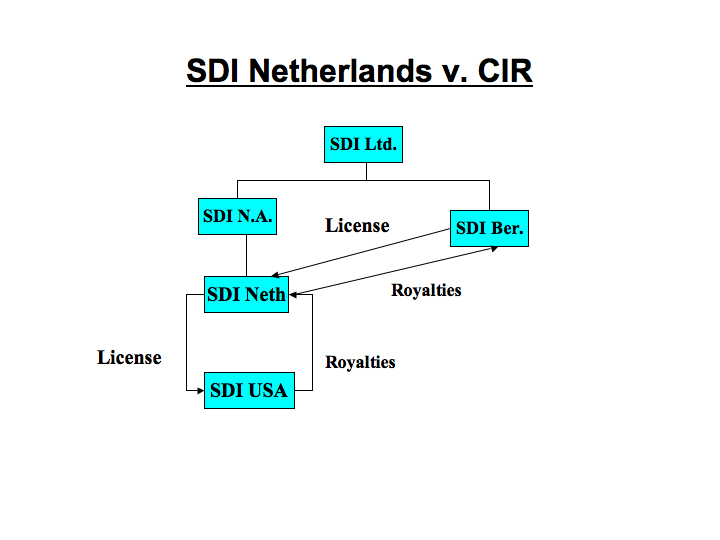
\includegraphics[width=140mm, height=80mm, clip, trim= 5mm 5mm 5mm 20mm]{SDI.png}}
\end{center}
\label{SDI}
\end{figure}

SDI Ltd. provided management services to certain of its direct and indirect subsidiaries for which such subsidiaries paid it management fees. 

\begin{center} \textbf{Royalty Payments Made By Petitioner}
\end{center}
During the years in issue, petitioner licensed from SDI Bermuda, pursuant to a license agreement dated 
November 28, 1986 (Bermuda license agreement), the worldwide rights to certain commercial systems software for use on IBM mainframe computers (the software). The Bermuda license agreement granted petitioner a nonexclusive license to use or to market the use of, on a worldwide basis, all of the software and any and all industrial and intellectual property rights SDI Ltd. had or would acquire from the effective date of the agreement \ldots, in exchange for certain royalty payments. The agreement further provided that petitioner ``shall specifically have the right to grant sublicenses and Agents for the right to use and to market the use of any and all marketing rights granted to [petitioner] under the terms'' of the agreement. The agreement was valid for an indefinite period and could be unilaterally terminated by either party on 3 months' written 
notice. 

The Bermuda license agreement contained no express reference to the United States. 

With respect to royalties, the Bermuda license agreement provided:
\begin{quote} 
8.1 The royalties payable to [SDI Bermuda] by [petitioner] under this Agreement are fixed at 93\% of 
the net amount of all of the royalties due to [petitioner] by all persons, entities and institutions which 
[petitioner] sublicensed any of the rights licensed to [petitioner] under this Agreement (``Sublicensees''). The 
aforementioned net amount is the amount that remains after the deduction of the withholding tax on royalties 
to be withheld when the Sublicensees of [petitioner] or Agents of [petitioner] pay the royalties due to the 
[petitioner].

[The 93\% rate was increased to up to 98\% if the royalties exceeded certain amounts.] 

\ldots
\end{quote} 
[From 1987 through 1990, SDI Netherlands paid between \$3.5 million and \$5.4 million annually to SDI Bermuda.  Those payments constituted roughly 94\% of the total worldwide royalty payments received by SDI Netherlands.]

\begin{center} \textbf{Royalty Payments Received by Petitioner from SDI USA }
\end{center}
During the years in issue, petitioner was a party to an exclusive license agreement with SDI USA, dated October 1, 
1972, and as modified from time to time, regarding the use and licensing of the software in the United States (the U.S. 
license agreement). \ldots SDI USA was responsible for the direct marketing and sales of the software in the United States. 

The U.S. license agreement provided in part:
\begin{quote} 
2.1 In consideration for the payment of the royalties provided hereunder and the performance of the other 
terms and conditions hereof by [SDI USA], [petitioner] hereby grants and transfers to [SDI USA], upon  the terms and subject to the conditions hereinafter set forth, the exclusive right and license during the Term hereof, to have disclosed to it by [petitioner] and to exploit, use and lease and otherwise obtain the benefit of [the software] within the Territory.

2.2 This Exclusive License shall include, (i) the right to sublicense to others the use and lease of [the 
software] within the Territory, subject, however, to the terms and conditions of this License; and (ii) this 
License shall also include the right and, as hereinafter provided, the obligation of [SDI USA], to provide or 
to provide for the exclusive maintenance, servicing and repair of [the software] within the Territory. * * * 
* * * * 

2.4 The Territory of this License shall mean and be restricted to the continental United States, Hawaii and 
Alaska. 
\end{quote}
Petitioner agreed not to license the software for use or to compete directly or indirectly with SDI USA's exploitation \margit{Should there have been an allocation to the non-compete?}
of the software in the United States during the term of its license to SDI USA. \ldots

Until February 1987, the agreement provided that SDI USA would pay to petitioner ``an annual royalty equal to fifty 
percent (50\%) of the annual gross revenues of [SDI USA] from leasing and sublicensing of [the software], 
without any deductions therefrom except rebates, discounts and sales or value added taxes.''
 
The U.S. license agreement was modified in February 1987 to provide that SDI USA would pay petitioner ``a royalty 
equal to (50\%) fift[y] percent of the gross billable or invoiced revenues of [SDI USA] with regard to all products licensed 
herein or further licensed in the future, without any deductions therefrom except rebates, or, sales or value added taxes.'' 

[SDI Netherlands received annual royalty payments from SDI USA from 1987-1990 of roughly \$2.5 million annually.]

\ldots 
 
\begin{center} \textbf{Discussion}
\end{center}
\ldots
\begin{center} \textbf{Liability for Withholding }
\end{center}

Section 881(a) provides that a 30-percent tax shall be imposed on ``the amount received from sources within the 
United States by a foreign corporation'' falling within certain categories of income. \ldots Section 1442 provides a method 
for collecting that tax. 

\ldots 
%Section 1442 provides in part:
%\begin{quote} 
%(a) General Rule.--In the case of foreign corporations subject to taxation under this subtitle, there shall 
%be deducted and withheld at the source in the same manner and on the same items of income as is provided 
%in section 1441 a tax equal to 30 percent thereof. * * *
%\end{quote} 
%Royalties are among the types of income included in section 1441(b). Sec. 1.1441-2(a), Income Tax Regs.; see also 
%sec. 1.881-2(b), Income Tax Regs. In addition, section 861(a)(4) provides that U.S. source income includes:
%\begin{quote} 
%(4) Rentals and Royalties.--Rentals or royalties from property located in the United States or from any 
%interest in such property, including rentals or royalties for the use of or for the privilege of using in the United
%States patents, copyrights, secret processes and formulas, good will, trade--marks, trade brands, franchises, 
%and other like property.
%\end{quote} 
%Section 1441(a) completes the picture of the statutory provisions involved herein. It provides: 
%\begin{quote}
%all persons * * * having the control, receipt, custody, disposal, or payment of any of the items of income 
%specified in subsection (b) [which includes ``royalties''] (to the extent that any of such items constitutes 
%gross income from sources within the United States), of any nonresident alien individual or of any foreign 
%partnership shall * * * deduct and withhold from such items a tax equal to 30 percent thereof * * * 
%\end{quote}
There can be no dispute that the royalty payments received by petitioner from SDI USA constitute U.S. source income and were received by petitioner as such within the meaning of section 1442(a). \ldots There is no comparable U.S. treaty exemption that would apply to royalty payments from SDI USA to SDI Bermuda. 

The parties have locked horns on several aspects of the application of the statutory provisions in light of the impact of 
the U.S.--Netherlands treaty exemption: (1) Whether the royalties paid by petitioner to SDI Bermuda constitute income 
``received from sources within the United States by'' SDI Bermuda and are thus subject to withholding under section 
1441(a);\ldots

%(2) whether petitioner can be considered a ``withholding agent''; (3) whether there is a limitations period that 
%has expired in respect of respondent's right to assess a deficiency in withholding tax against petitioner; and (4) whether 
%petitioner is liable for additions to tax under section 6651(a)(1) for failure to file withholding tax returns. 

For reasons hereinafter set forth, we resolve the first issue in petitioner's favor with the result that it is unnecessary for 
us to address the remaining issues. \ldots Before proceeding with our analysis of the first issue, however, it is important to 
note that respondent does not question the existence of petitioner as a valid Netherlands corporation or the application of 
the treaty exemption insofar as the payments by SDI USA to petitioner are concerned. Similarly, respondent does 
not attack the arrangements under which petitioner had a license of the worldwide rights and SDI USA had a license of 
the U.S. rights, although respondent does ask us to take into account the close relationship of the various corporations 
involved. \ldots

Rather, respondent focuses her argument solely on the proposition that, since the royalties paid by SDI USA to 
petitioner were U.S. source income, they retained that character as part of the royalties paid by petitioner to SDI 
Bermuda and, as a matter of law, constitute income ``received from sources within the United States by'' SDI Bermuda 
under section 881(a). \ldots Respondent contends that the fact that such royalties were combined with non--U.S. source 
royalties  received by petitioner to determine the amount of royalties payable by petitioner to SDI Bermuda 
does not preclude the tracing of the royalties received by petitioner from SDI USA to U.S. sources. \margit{The IRS argues that royalties do not change source when paid through chains of sublicensees.} To implement such 
tracing, respondent simply applies the percentage specified in the worldwide license agreement between petitioner and 
SDI Bermuda and utilized in computing the amount of the required payment by petitioner to SDI Bermuda. \ldots In all of [the cases cited by the CIR], however, the payments, upon which a 
withholding tax was imposed, were directly from a U.S. payor and the U.S. withholding tax was imposed on that payor. 
None of them address the situation involved herein, where there is a second licensing step under which royalties are being 
paid and upon which the U.S. withholding tax is sought to be imposed. Thus, these cases provide no guidance in respect
of whether the U.S. source characterization of the royalties paid by SDI USA to petitioner flows through to the royalties 
paid by petitioner to SDI Bermuda. 

Petitioner argues that the royalties paid by SDI USA to petitioner and exempt from tax under the Netherlands treaty 
became merged with the other royalties received by petitioner from non--U.S. sources and consequently lost their character 
as U.S. source income. Petitioner submits that, while the royalty payments from SDI USA may be U.S. source 
income, its royalty payments to SDI Bermuda were made on a separate and independent basis. With respect to the 
payments to SDI Bermuda, petitioner contends that they were made pursuant to a worldwide licensing agreement between 
two foreign corporations, and as such do not constitute income ``received from sources within the United States'' so that 
no withholding is required under section 1442(a). 
Pertinent authority on the issue before us is sparse. Indeed respondent relies solely on Rev.\@\@ Rev.\@\@ 80--362, 1980--2 C.B. 
208, for her ``flow--through'' position. \ldots 
 
We are not persuaded that Rev.\@\@ Rul.\@\@ 80--362, supra, \margit{Note the lack of deference the Tax Court accords revenue rulings.} provides any significant support for respondent's position herein. It 
fails to reflect any reasoning or supporting legal authority. This circumstance is particularly relevant in applying the usual 
rule that, in any event, revenue rulings are not entitled to any special deference. \ldots 
 
At this point, we note that respondent has not argued that petitioner was a mere conduit or agent of SDI USA in paying 
royalties to SDI Bermuda or that SDI Bermuda was the beneficial owner of the royalties petitioner received from SDI USA 
so that the U.S.--Netherlands treaty exemption should not apply. \ldots Presumably such an argument would have produced a situation 
where SDI USA rather than petitioner would have been targeted by respondent as the taxpayer liable for the withholding 
tax under section 1442(a). \ldots 

Although [Aiken and Northern Indiana] involved the conduit concept, we think they provide some guidance for our disposition of the instant 
case. We take this view because the flow--through characterization concept is, in a very real sense, the conduit concept 
albeit in a somewhat different garb, i.e., whether the U.S. source income is being received as such, because of the status 
of the paying entity in one case, and the status of the subject matter of the payment in the other.

In [Aiken], back--to--back loans, in the identical amounts of principal and rates 
of interest, were made between a U.S. corporation and a related corporation organized under the laws of the Republic 
of Honduras, and between the Honduran corporation and its indirect parent. Respondent argued that the Honduran 
corporation should be disregarded for tax purposes, and that the parent corporation should be deemed the true owner 
and recipient of the interest payment from the U.S. corporation. We held the Honduran corporation to be a mere 
conduit for the passage of interest payments and imposed withholding tax liability on the U.S. corporation.
 
In [Northern Indiana], the taxpayer, a domestic corporation, organized a 
finance subsidiary incorporated in Curacao under the Commercial Code of the Netherlands Antilles, (to which the U.S.-- 
Netherlands treaty applied) for the purpose of issuing notes in the Eurobond market. The finance subsidiary borrowed 
\$70 million at 17--1/4 percent interest in that market and lent that amount to the taxpayer at 18--1/4 percent interest. 
Respondent argued that the finance subsidiary should be ignored and that the taxpayer was liable for withholding taxes 
under section 1441 on the interest payments to the foreign Eurobond holders. Finding that the finance subsidiary engaged 
in substantive business activity that resulted in significant earnings, we held that the finance subsidiary was not a mere 
conduit or agent. 

We think the within situation falls more within the ambit of Northern Indiana than Aiken Industries. In the 
latter case, there was an identity both in terms and timing between the  back to back loans, as well as a close 
relationship between the parties involved. In the former case, although there was a clear connecting purpose between 
the borrowing and lending transactions, \emph{i.e.}, to obtain the benefit of the exemption from the withholding tax on interest 
under the U.S.--Netherlands treaty; there were differences in terms, \emph{i.e.}, in the interest rate (albeit not large); and a close 
relationship between all the parties was not present since the borrowings by the finance subsidiary were from unrelated 
parties. 

In the instant case, there was a close relationship between the parties. However, although respondent asks us, in 
passing, to take that relationship into account, she does not pursue the matter to the point where she contends that it is a 
significant factor. Given the fact that respondent recognizes the existence of all of the parties as valid corporate entities and 
does not attack the bona fides of the license agreements between SDI USA and petitioner, on the one hand, or petitioner 
and SDI Bermuda, on the other, we are not disposed to allow the close relationship element to control our decision. 

The facts of the matter are that the two license agreements had separate and distinct terms and that petitioner 
had an independent role as the licensee from SDI Bermuda and the licensor of the other entities, including but not 
limited to SDI USA. The schedules of royalty payments provides for a spread, not unlike the spread involved in Northern 
Indiana, which compensated petitioner for its efforts. Like the finance subsidiary in Northern Indiana, petitioner engaged 
in licensing activities from which it realized substantial earnings. In fact, on a percentage basis, it earned between 5 and 6 
percent, compared to the 1 percent earned by that finance subsidiary in Northern Indiana. \ldots Under the circumstances 
herein, we think these arrangements should be accorded separate status with the result that, although the royalties paid 
by petitioner to SDI Bermuda were derived from the royalties received by petitioner from SDI USA, they were \margit{Did the court get sidetracked with the conduit argument?}  
separate payments. 

We find support for our conclusion herein in that respondent's view of the law could cause a cascading royalty 
problem, whereby multiple withholding taxes could be paid on the same royalty payment as it is transferred up a chain of 
licensors. \ldots  But for the U.S.--Netherlands treaty, the royalty 
payments from SDI USA could be subject to withholding tax twice under respondent's reasoning herein. 

Respondent argues that only one withholding tax is being sought herein. However, this ignores the fact that, by 
treaty, the U.S. agreed to forgo taxing royalties and to allow them to be taxed by The Netherlands. Whether or not The 
Netherlands actually taxed the royalties is irrelevant. 
Respondent also infers that she would use her discretion not to apply more than one level of withholding tax on
multiple transfers of income that originated as U.S. source income. We think this  places an improper exercise of 
discretion in respondent's hands. To avoid the imposition of interest and additions to tax as determined by respondent 
herein, each payor in the chain might well feel compelled to file returns and pay withholding taxes. \ldots  We are not disposed to 
conclude, in the absence of any legislative expression on the subject, that Congress intended the statutory provisions to 
permit ``cascading'' with the question of relief left to the mercy of respondent. 

We hold that the payments by petitioner with respect to which respondent seeks to impose liability for the 30 percent 
withholding tax herein were not ``received from sources within the United States by'' SDI Bermuda under sections 881(a), 1441(a), and 1442(a).\footnote[17]{ 
We note that changes in the U.S.--Netherlands treaty, applicable to years subsequent to the years before us, 
may provide a different framework for disposing of this issue. \ldots }

Decision will be entered for petitioner.
\end{select}

In commercial contracts, it is not uncommon to designate an amount as a royalty if it is determined by reference to future sales.  For example, an author can be paid a fixed amount and a ``royalty'' based on the total sales of his book.  This is often an efficient arrangement if the parties cannot agree \emph{ex ante} on the value of the author's service.  The tax issue that arises is whether such an amount is truly a royalty or instead a payment for services.  The following cases, \emph{Ingram v.\@ Bowers} and \emph{Pierre Boulez v.\@ CIR}, address this issue.  What can potentially happen to a taxpayer if one country taxes income as services and the other as royalties?  


\addcontentsline{toc}{section}{\protect\numberline{}Ingram v.\@ Bowers} 
\begin{select}
\caseart{Ingram v.\@ Bowers}{ 47 F.2d 925 (S. D. N. Y. , 1931) }{PATTERSON, Judge}\\

\ldots 

The case concerns the taxability of income received by 
Caruso by reason of the sale of phonograph records outside the United States, it being conceded that the singing 
by Caruso for the manufacture of such records occurred 
within the United States. The plaintiff contends: First, 
that Caruso was a nonresident alien, a proposition which 
the defendant disputes; and, second, that the amounts in 
question were not income from sources within the United 
States, which the defendant also disputes. 

Caruso was the foremost singer of the world. His fame 
was international, although the greater part of his singing 
during the last ten years of his life was done in the United 
States. He was born in Italy and always remained a subject of that country. For many years prior to his death in 
1921, he spent about six months of the year in the United 
States, singing at the Metropolitan Opera House in 
New York City and giving concerts at other cities. At the 
close of the operatic season, he almost always returned 
to Italy, where he maintained a large estate. His headquarters in the United States were the Knickerbocker Hotel, 
New York City, where he leased a suite of rooms, and 
later the Vanderbilt Hotel here. He married the plaintiff 
here in 1918, and in 1919 a daughter was born here. His 
income from opera and concert work in the United States 
was large and in making income tax returns he always 
claimed the status of a nonresident alien. During his lifetime, no question seems to have been raised as to this 
being his real status. 

Among his other engagements, Caruso was under contract with the Victor Talking Machine Company, a New 
Jersey corporation, to sing for the purpose of enabling the 
Victor Company to make phonograph records of selections rendered by him. By contract dated April 3, 1909, 
he agreed to sing selections at the Victor laboratories in 
Camden, the Victor Company to pay him a royalty of 50 
cents on each larger record and a royalty of 25 cents on 
each smaller record of his voice which it should sell. The 
contract was to continue for twenty--five years and 
was exclusive in the sense that Caruso bound himself not 
to sing for the purpose of making phonograph 
records for any one else.\margit{Note the noncompete and failure to allocate any of the payments to the noncompete.} On January 1, 1919, this contract was superseded by a new one, under which Caruso 
was to render forty selections at the Victor laboratories. 
The Victor Company bound itself to pay Caruso a royalty 
equal to 10 per cent. of its list price on all records of his 
voice which should be sold, and it ``guaranteed'' a minimum payment of \$100,000 a year during his life but not 
to exceed ten years. (It may be noted here that for the 
remainder of Caruso's life the royalties on the percentage 
basis were far in excess of \$100,000,\margit{This amount is equivalent to \$1.37 million in 2012 dollars.} so that the ``guaranty'' did not become operative.) The 1919 contract also 
contained a provision to the effect that Caruso would not 
permit any records of his voice to be made by any other 
concern. 

In performance of these successive contracts, Caruso 
would go to Camden and sing operatic selections. The 
sound would be recorded on wax, from which a master matrix would be made. From this master matrix the 
records for sale in the United States were manufactured. 
Records of Caruso's voice were also sold in other 
countries under the Victor contracts, and it is in relation to 
the royalties measured by sales in these countries that the 
present case arises. By contracts with companies doing 
business in Canada and in England, the Victor Company 
agreed to furnish such companies with matrices of its selections. One of the terms as to payment by the foreign 
companies was that they should pay the Victor Company 
all royalties which the latter was called upon to pay the 
artist. Pursuant to such contracts, the Victor Company 
sent various matrices of songs by Caruso to the foreign 
companies, and in due course they credited the Victor 
Company with sums of money representing the royalty 
which the Victor Company was obligated to pay Caruso, 
the amounts depending of course upon the number of 
records sold by the foreign companies. These sums were 
credited to Caruso on the Victor books and were paid to 
him along with the payments for records sold within the 
United States. 

%Upon an audit of Caruso's income tax return for 1918, 
%the commissioner added the sum of \$18,536.25 to his 
%taxable income as the amount received by him from the 
%Victor Company because of the sales of records abroad. 
%The tax thereon was \$13,924.69. Similarly for the 
%year 1919, the sum of \$1,789.75 was added to income, 
%and a further tax of \$1,086.86 was assessed. Similarly for 
%1920, the sum of \$36,400.59 was added to income, and 
%a further tax of \$25,844.42 was assessed. The plaintiff 
%paid these amounts, totaling \$40,855.97, under protest 
%and brought this action to recover them. 
%Section 213(c) of the Revenue Act of 1918 (40 Stat. 
%1066) deals with nonresident aliens and provides that in 
%their case ``gross income includes only the gross income 
%from sources within the United States.''
 
%The first issue is whether Caruso was a resident alien 
%or a nonresident alien during the three years in question. 
%If he was a resident alien, he was taxable upon his entire 
%net income, irrespective of source. But I have no doubt 
%that his status was that of a nonresident. His original residence was in Italy, and there is no satisfactory evidence 
%of an intention to abandon that residence. His stays in the 
%United States were transitory and, except for one or two 
%occasions, were only for the purpose of fulfilling operatic 
%and concert engagements. Granting that domicile and residence are not synonymous under the income tax 
%statutes [Bowring v.\@ Bowers (C.C.A.) 24 F.(2d) 918], I am 
%persuaded that Caruso's residence as well as his domicile 
%was in Italy. He was therefore taxable only on income 
%from sources within the United States. 

The [source of income from the foreign sales] is not so easy of solution. Did the 
moneys received by Caruso on account of foreign sales of 
records constitute income from sources within the United 
States? I have reached the conclusion that they did. The 
contracts which Caruso made with the Victor Company 
were contracts requiring him to render services. They 
called upon him to sing for Victor and to refrain from 
singing for any other phonograph company. For this he 
was to be paid by Victor according to the number of 
records sold, with a minimum compensation to be paid 
in any event. The contracts were in no sense contracts of 
sale or of license. Caruso had no proprietory right, title, 
or interest in the matrices or in the records. It is true that 
compensation was measured, in part at least, by the number of records sold and was referred to as a royalty; but 
the fact remains that the arrangement was one to render 
services in his capacity as a singer, as thoroughly as if the 
compensation had been a set sum.
 
The services rendered by Caruso were rendered in the 
United States. I think that this is the decisive feature. 
Those services were the source of all his income derived 
from the Victor contracts. It cannot be denied that but 
for the sales abroad part of this income would not have 
accrued. An event in a foreign country was necessary 
before the income became payable. But this 
cannot obscure the fact that the source, the origin of the 
income was Caruso's singing in Camden, N.J. I cannot 
see any difference in principle between this case and a 
case where a lawyer performs services in New York on a 
lawsuit pending in London, his compensation to be contingent upon success in the lawsuit. No income is realized 
until the happy issue of the suit in London, but clearly the 
source of the income, when realized, was the work done 
in New York. Or suppose a nonresident alien spends a 
year in New York working as sales manager for a merchandising company, his compensation to be a percentage 
of the proceeds of sales, and part of the sales are made in 
Canada and Mexico. Beyond doubt his earnings represent 
income from sources within the United States, where all 
his work was done, despite the fact that the amount 
of his earnings was enhanced by sales which took place 
in foreign countries. The same is true here. It seems to 
me that where a singer makes and performs in the United 
States a contract to sing for a phonograph company, for 
which he is to be paid a fixed sum for each record sold 
or a percentage of the list price of the records sold, the 
compensation so received is income from sources within 
the United States; the fact that some of the sales were 
made in foreign countries is immaterial. 

\ldots 
%I have considered the cases holding that where a life 
%insurance agent has obtained policies in earlier years, under an agreement with the insurance company that he is 
%to receive a commission out of all renewal premiums on 
%such policies, such commissions received by the agent 
%in later years will be deemed income for the years when 
%received. Edwards v.\@ Keith (C.C.A.) 231 F. 110; Woods 
%v.\@ Lewellyn (C.C.A.) 252 F. 106. These cases stand for 
%the proposition that where a person performs services for 
%compensation conditionally promised, no income is realized until such time as the condition is performed; the 
%time when the work was done is unimportant. The proposition is clearly a sound one and would apply to the present situation if there were any question as to the time 
%when Caruso received income under the Victor contracts. 
%See, also Zimbalist v.\@ Anderson (D.C.) 23 F.(2d) 328, affirmed in (C.C.A.) 38 F.(2d) 57. But here the question is 
%one of place, not of time; the search, under the terms of 
%section 213(c) of the Revenue Act 1918, is for the territorial source of the income. And, as already pointed out, 
%it seems to me that the place where the work is done, and 
%not the place where the later event fixing compensation 
%occurs, is the source of the income, in cases where the 
%income is from the exercise of a profession or vocation as 
%in this case. 

%I have already said that the controlling fact is that 
%Caruso's part in the making of the records was performed 
%in this country. There are, however, other elements in the 
%case which reinforce the conclusion that the source of this 
%income was within the United States. It was the reputation which Caruso had won by his operatic and concert 
%successes in the United States that led to the making of 
%the Victor contracts. It was here that the contracts were 
%made. It was here that the payments under the contracts 
%were made. The payments were the obligation 
%of a company incorporated and doing business here. The 
%fact that the foreign sales were made by other companies 
%is of no consequence; the situation is the same as if Victor 
%had made such sales directly. It would have been accountable to Caruso for the agreed amount or percentage in any 
%event, even if it had received nothing from its contractors 
%in England and Canada. 

My conclusion is that the income was from sources 
within the United States and was therefore taxable. A 
verdict for the defendant is accordingly directed.
\end{select}

\addcontentsline{toc}{section}{\protect\numberline{}Ingram v.\@ Bowers} 
\begin{select}
\caseart{Ingram v.\@ Bowers}{ 57 F.2d 65 (2nd Cir. 1932) }{L. Hand, Circuit Judge}\\

\ldots 

%The case turns upon the meaning of the phrase, ``gross 
%income from sources within the United States,'' as used 
%in section 213(c) of the Revenue Act of 1918 (40 Stat. 
%1066); for we assume arguendo that, as the judge found, 
%Caruso was a non--resident alien. If his agreements with 
%the Victor Company were no more than contracts for personal services, it makes no difference whether we hold, 
%as was held below, that the source of the resulting income 
%was the services rendered,  or the promise to pay 
%the royalties. The first has the authority of a departmental 
%ruling (Cum. Bul. Dec. 1920, p. 128), and whatever infer- 
%ences may be drawn from the amendments in the statutes 
%from 1921 forward (section 217(a)(3) of the Acts of 1921 
%(42 Stat. 244) and 1924 and 1926 (26 USCA � 958(a)(4); 
%� 119(a)(3) of 1928, 26 USCA � 2119(a)(3). On the other 
%hand we find it difficult to distinguish Edwards v.\@ Keith, 
%231 F. 110 (C.C.A. 2) and Woods v.\@ Lewellyn, 252 F. 
%106 (C.C.A. 3). A priori, the source of an income would 
%seem to be determined by the same factors, whether time 
%or place be in question; if that source is the consideration 
%for the promise, and not the promise itself, the return for 
%services rendered before any tax was imposed would not 
%be a gain from any taxable source. However, we are not 
%driven to a decision on this point, because if the source 
%is the promise, the promisor was also within the United 
%States, and the same result follows as though the service 
%was the source. 

The more vital question is whether the contracts were 
for more than personal services; whether they gave to 
Caruso some interest in the matrices and records, or, if 
there was any copyright, in the copyright; and 
whether the payments can in this wise be looked at as 
emanating from property. If so, the plaintiff argues, the 
sums in suit came from the foreign matrices; if not, then 
at least from the foreign companies. As to both matrices 
and records the second contract is too clear for question; 
it provides that Caruso ``grants all rights in and to'' them. 
The first contract contained no such words, but we think 
that the result was the same. In it he only agreed ``to 
make these records,'' meaning of course, to sing into the 
recording apparatus, and the Victor Company, to pay him 
a royalty as records made from the resulting matrices were 
sold. The company was to manufacture both; prima facie 
they became its chattels like anything else of its mak[ing]. If 
it was intended to give Caruso an interest in them, some 
such reservation was to be expected, and there was none. 
The fact that his return was called a royalty is immaterial; 
it was so described in the second contract which was not 
equivocal. No remedy was created by which he could 
assert any such rights. It appears to us that the purpose 
was the same as was expressed later, and if so, he had 
no proprietary interest in the profits arising out of
the records. If there be a copyright under section 1(e) of 
the Copyright Act (17 USCA \S 1(e)---which we 
do not say---it became embodied in the matrices, as a 
literary composition is embodied in its text. Any putative 
monopoly would do no more than prevent the copying 
of these, and it passed with the property in them. It was 
not impliedly reserved separate from them, for that would 
have interfered with their full enjoyment which the manufacturer was certainly to have. 

Nor can we see how the source of the payments could 
be the royalties paid by the foreign companies to the 
Victor Company. They did not promise to pay Caruso, 
or to assume the obligations of the company.Whether in 
the event of its insolvency, he could have had recourse to 
their promises is beside the mark. Assuming as much, 
it would be only as security for the Victor Company's 
performance, and that would not change the source of 
the income while it continued to perform. For argument 
we may even assume the contrary after default; it never 
did default; all the payments here in question came from 
it. This would be equally true, though by a long stretch 
we were to assimilate the situation to that in Re Waterson, Berlin \& Snyder Co., 48 F.(2d) 704 (C.C.A. 2), and hold that Caruso had a lien upon the matrices sent 
to the foreign companies. That would again be only as 
security, for under the doctrine of that decision the second assignee does not, by accepting the transfer, become 
personally liable on the promise of the first. As long as 
the first assignee performs, the assignor's rights against 
the second remain in abeyance; if he defaults, they are 
against the property alone. Thus, on no theory can it be 
said that the source of this income was outside the United 
States. 

Judgment affirmed.
\end{select}
In the \emph{Boulez} case below, the same issue---whether income related to the sale of property produced by personal services is royalty income or compensation---arises in the context of a well-known conductor who is a treaty resident.

\addcontentsline{toc}{section}{\protect\numberline{}Pierre Boulez v.\@ CIR} 
\begin{select}
\caseart{Pierre Boulez v.\@ CIR}{ 83 T.C. 584 (1984) }{Korner, Judge}\\
\ldots
\begin{center}
\textbf{ FINDINGS OF FACT}
\end{center} 
The petitioner, Pierre Boulez, resided in Paris, France, at the time the petition was filed in this case. Petitioner is 
a citizen of France, and during the calendar year 1975 was a resident of the Federal Republic of Germany 
(hereinafter FRG). For the taxable year 1975, petitioner was a nonresident alien of the United States for Federal 
income tax purposes, and he timely filed a Federal nonresident alien income tax return for that year with the Office of International Operations of respondent. 

At all times relevant to this case, petitioner was a world--renowned music director and orchestra conductor. On 
February 19, 1969, petitioner entered into a contract with CBS Records, a division of CBS United Kingdom, Ltd., which 
is a subsidiary of CBS, Inc., a U.S. corporation. Said contract was modified as of September 13, 1971, and March 14, 
1974, and, as so modified, was in effect during the year 1975. Under date of May 1, 1972, with the consent of CBS 
Records, the contract was assigned by petitioner to Beacon Concerts, Ltd., of London England, which acted as petitioner's 
agent and undertook to provide his services to CBS Records under the terms of the basic contract, as amended. 
As relevant and material herein, the contract between petitioner and CBS Records, as in effect in the year 1975, 
provided in part as follows:
\begin{quote} 
1. We [CBS Records] hereby agree to engage and you [the petitioner] agree to render your services exclusively for 
us as a producer and/or performer for the recording of musical and/or literary compositions for the purpose of 
making phonograph records. It is understood and agreed that such engagement by us shall include your services as a 
producer and/or performer with the New York Philharmonic for the recording of musical and/or literary compositions for 
the purposes of making phonograph records. 

* * * *
 
3. (a) During the first two contract years of this agreement you will perform for the recording of satisfactory master 
recording [sic] sufficient in number to constitute two (2) 12 inch long playing 33 1/3 rpm recordings, or their equivalent, 
and we will record your performances; and during each contract year commencing September 13, 1971, you will perform 
for the recording of satisfactory master recordings sufficient in number to constitute three (3) twelve inch long--playing 
33 1/3 rpm recordings, or their equivalent, and we will record your performances. Additional master recordings will be 
performed by you and recorded by us at our election. 

* * * *
 
4. During the period of this Agreement you will not for any reason whatsoever give or sell your services under your 
own or any assumed name or anonymously to any other person firm or corporation but nothing herein 
contained shall preclude you for [sic] giving or selling your services for films personal appearances and broadcasting 
(whether or not accompanied by television) provided such services are not reproduced as records for sale to the public 
and you undertake to have this proviso included in any contract for such services. \margit{Note the existence of a covenant not to compete and the failure to allocate any income to this covenant.} You will not during the period of five 
years after the expiration of the term of this Agreement give or sell your services for the purpose of making or assisting in 
the making of records of any of the compositions or works which you shall have performed under this Agreement. You 
acknowledge that your services are unique and extraordinary and that we shall be entitled to equitable relief to enforce 
the provision of this paragraph 4. 

5. All master recordings recorded hereunder and all matrices and phonograph records manufactured therefrom, 
together with the performances embodied thereon, shall be entirely our [CBS Records] property, free from any claims 
whatsoever by you [petitioner] or any person deriving any rights or interests from you. Without limiting the generality of 
the foregoing, we (including other divisions of our company) and/or our subsidiaries, affiliates and licensees shall 
have the unlimited right, from time to time, to manufacture, by any method now or hereafter known, phonograph records 
and other reproductions, on any mediums or devices now or hereafter known, of the master recordings made hereunder, 
and to sell transfer or otherwise deal in the same throughout the world under any trademark, trade names and labels or to 
refrain from such manufacture, sale and dealing; 

* * * *
 
6. We hereby agree to pay the accompaniment costs and studio charges in connection with the master recordings made 
hereunder.
 
* * * *
 
13. If, by reason of illness, injury, accident or refusal to work, you fail to perform for us in accordance with the 
provisions of this agreement, * * * we shall have the option without liability to suspend the application of paragraph 2 
and/or paragraph 7 (including the payment of any royalties) of this agreement for the duration of any such contingency by 
giving you written notice thereof. 
\end{quote}

Under paragraph 7a of the contract, it was provided ``For your services rendered hereunder and for the rights granted to 
us herein we will pay you the following royalties.'' There then followed an elaborate formula by which the petitioner was to be paid, based upon a percentage of the retail price derived by CBS Records from the sale of its phonograph 
records produced under the contract, with said percentage varying depending upon various factors, including, inter alia, 
whether the musical composition involved was in the public domain, whether the performance conducted by 
petitioner was made with the New York Philharmonic Orchestra, whether sales were made by direct sales or mail order 
through what was termed a ``Club Operation,'' whether the record involved was a ``re--issue,'' etc. In all cases, however, 
the payments or ``royalties'' which petitioner was to be entitled to receive were dependent upon future sales of recordings 
by CBS Records. 

Pursuant to the February 19, 1969, contract with CBS Records, as amended, petitioner conducted various performances 
with the Cleveland Orchestra, the New York Philharmonic, and others in the recording of musical compositions for CBS 
Records. None of these recordings were from ``live'' performances (i.e., performances before an audience). They were 
all private performances arranged solely for purposes of recording. CBS, Inc., was responsible for and exercised 
control over the setting up of the recording session, employing and paying the members of the orchestra, providing and 
arranging the equipment and engineers and technicians needed to capture and electronically process the sounds rendered 
by the orchestra, and for compiling and editing the sounds to make master recordings, matrices, and phonograph records. 
Petitioner exercised control over the manner in which the orchestra transposed into aural form the underlying musical 
composition which was the subject of each recording. He determined the placement of the musicians and the volume 
of aural sound to be rendered by the various musical instruments making up the orchestra. In conducting the orchestra, 
petitioner exercised his individual artistic talents of interpreting the musical work. Such interpretation, which is the 
function of the conductor, differs from conductor to conductor and is unique to each conductor's recording of a particular 
work. 

Applications for the copyrights of all the master recordings, matrices, and phonograph records embodying the sound 
recordings of the musical compositions conducted by petitioner pursuant to the contract were filed by CBS, Inc., 
and all registrations thereof were issued by the U.S. Copyright Office registered in the name of CBS, Inc. 
As the result of performances conducted by petitioner under the terms of the contract, CBS, Inc., paid to Beacon 
Concerts, Ltd., as petitioner's agent, the sum of \$39,461.47 in the year 1975. Beacon Concerts, Ltd., in turn, paid 
such sum to petitioner in 1976. In his 1975 U.S. nonresident alien income tax return, petitioner disclosed the receipt of 
such amount, but excluded it as not being subject to U.S. income taxation. Petitioner reported the identical amount in his 
1976 income tax return filed with the FRG as includable income subject to the German income tax, and petitioner paid 
German income tax thereon. 

Upon audit of petitioner's 1975 U.S. income tax return, respondent determined, inter alia, that the entire amount of 
\$39,461 was taxable to petitioner by the United States. Because of an apparent conflict between respondent and the FRG 
concerning the proper taxation of this income under the existing income tax treaty between the United States and the 
FRG, competent authority proceedings, pursuant to the provisions of the treaty, were instituted at the request of 
petitioner and were conducted by the FRG Ministry of Finance and respondent's Office of International Operations in an 
effort to resolve the issues arising under said income tax treaty. 

The competent authorities of the two nations were unable to reach agreement on the correct treatment for income tax 
purposes of the income here involved. The position of the FRG was that these payments constituted ``royalties,'' within the 
meaning of article VIII of the treaty, and therefore were taxable exclusively by the FRG. Respondent, on the other hand, 
took the position that said income was income from performance of personal services in the United States by petitioner, 
and therefore was taxable by the United States under the provisions of article X of said treaty, except that respondent here 
concedes that, of the total amount of \$39,461.47, the amount of \$9,000 was income from sources without the United 
States and was not subject to taxation by respondent, thus leaving the net amount of \$30,461 in issue.\ldots
\begin{center}
\textbf{ULTIMATE FINDING OF FACT}
\end{center} 
The payments of CBS, Inc., to petitioner in 1975 were payments as compensation for personal services rendered by petitioner.
\begin{center}
\textbf{OPINION}
\end{center} 
Petitioner contends that the payments to him in 1975 by CBS, Inc., were not taxable by the United States, because 
they were ``royalties'' within the meaning of the applicable treaty between the United States and the FRG. Respondent, 
as noted above, contends that the payments in question were taxable to petitioner by the United States because they 
represented compensation for personal services performed in the United States by petitioner. The parties are in agreement 
that the outcome of this dispute is governed by the effective income tax treaty between the United States and the FRG. \ldots  Petitioner, a resident of the FRG, was a person within the coverage of the treaty. The 
relevant portions of the treaty provide, in part: 
\begin{quote}
Article II \\
(2) In the application of the provisions of this Convention by one of the contracting States any term not otherwise 
defined shall, unless the context otherwise requires, have the meaning which the term has under its own applicable laws * * * 

* * * *
 
Article VIII \\ 
(1) Royalties derived by a natural person resident in the Federal Republic or by a German company shall be exempt 
from tax by the United States.\\ 
* * * * \\
(3) The term ``royalties'', as used in this Article, \\
(a) means any royalties, rentals or other amounts paid as consideration for the use of, or the right to use, copyrights, 
artistic or scientific works (including motion picture films, or films or tapes for radio or television broadcasting), patents, 
designs, plans, secret processes or formulae, trademarks, or other like property or rights, or for industrial, commercial or 
scientific equipment, or for knowledge, experience or skill (know--how) and 
(b) shall include gains derived from the alienation of any right or property giving rise to such royalties. \\
* * * * \\
Article X
 
* * * *
 
(2) Compensation for labor or personal services (including compensation derived from the practice of a liberal 
profession and the rendition of services as a director) performed in the United States by a natural person resident in the 
Federal Republic shall be exempt from tax by the United States if \ldots
\end{quote}
Acknowledging that the provisions of the treaty take precedence over any conflicting provisions of the Internal 
Revenue Code of 1954 (sec. 7852(d); see also sec. 894), we must decide whether the payments received by 
petitioner in 1975 from CBS, Inc., constituted royalties or income from personal services within the meaning of that 
treaty. This issue, in turn, involves two facets:
\begin{quote} 
(1) Did petitioner intend and purport to license or convey to CBS Records, and did the latter agree to pay for, a property interest in the recordings he was engaged to make, which would give rise to royalties? \\
(2) If so, did petitioner have a property interest in the recordings which he was capable of licensing or selling? 
\end{quote}
The first of the above questions is purely factual, depends upon the intention of the parties, and is to be determined 
by an examination of the record as a whole, including the terms of the contract entered into between petitioner 
and CBS Records, together with any other relevant and material evidence.

The second question--whether petitioner had a property interest which he could license or sell--is a question of law. 
The treaty is not explicit, and we have found no cases or other authorities which would give us an interpretation of the 
treaty on this point. We are therefore remitted to U.S. law for the purpose of determining this question. \ldots
  
\begin{center}\textbf{1. The Factual Question}
\end{center} 
By the contract entered into between petitioner and CBS Records in 1969, as amended, did the parties agree that 
petitioner was licensing or conveying to CBS Records a property interest in the recordings which he was retained to make, 
and in return for which he was to receive ``royalties?'' Petitioner claims that this is the case, and he bears the burden of 
proof to establish it. 

The contract between the parties is by no means clear. On the one hand, the contract consistently refers to the 
compensation which petitioner is to be entitled to receive as ``royalties,'' and such payments are tied directly to the 
proceeds which CBS Records was to receive from sales of recordings which petitioner was to make. Both these 
factors suggest that the parties had a royalty arrangement, rather than a compensation arrangement, in mind in entering 
into the contract. We bear in mind, however, that the labels which the parties affix to a transaction are not necessarily 
determinative of their true nature, and the fact that a party's 
remuneration under the contract is based on a percentage of future sales of the product created does not prove that a 
licensing or sale of property was intended, rather than compensation for services. 

On the other hand, the contract between petitioner and CBS Records is replete with language indicating 
that what was intended here was a contract for personal services. Thus, paragraph 1 (quoted in our findings of fact) 
clearly states that CBS Records was engaging petitioner ``to render your services exclusively for us as a producer and/or 
performer * * * It is understood and agreed that such engagement by us shall include your services as a producer 
and/or performer.'' Paragraph 3 of the contract then requires petitioner to ``perform'' in the making of a certain number of 
recordings in each year. Most importantly, in the context of the present question, paragraph 4 of the contract (quoted in 
our findings) makes it clear that CBS considered petitioner's services to be the essence of the contract: petitioner agreed 
not to perform for others with respect to similar recordings during the term of the contract, and for a period of 5 years 
thereafter, and he was required to ``acknowledge that your services are unique and extraordinary and that we shall be 
entitled to equitable relief to enforce the provision of this paragraph 4.''
 
Under paragraph 5 of the contract (quoted supra), it was agreed that the recordings, once made, should be entirely 
the property of CBS Records, ``free from any claims whatsoever by you or any person deriving any rights or interests 
from you.'' Significantly, nowhere in the contract is there any language of conveyance of any alleged property right in the 
recordings by petitioner to CBS Records, nor any language indicating a licensing of any such purported right, other than the designation of petitioner's remuneration as being ``royalties.'' The word ``copyright'' itself is never mentioned. 
Finally, under paragraph 13 of the contract, CBS Records was entitled to suspend or terminate its payments to petitioner 
``if, by reason of illness, injury, accident or refusal to work, you fail to perform for us in accordance with the provisions of 
this agreement.'' 

Considered as a whole, therefore, and acknowledging that the contract is not perfectly clear on this point, we conclude 
that the weight of the evidence is that the parties intended a contract for personal services, rather than one involving the 
sale or licensing of any property rights which petitioner might have in the recordings which were to be made in the future. 
\begin{center} \textbf{ 2. The Legal Question}
\end{center}
Before a person can derive income from royalties, it is fundamental that he must have an ownership interest in the 
property whose licensing or sale gives rise to the income. Thus, in Patterson v.\@ Texas Co., 131 F.2d 998, 1001 (5th Cir. 
1942), the Court of Appeals adopted the definition of a ``royalty'' as ``a share of the product or profit reserved by the 
owner for permitting another to use the property.'' Likewise, in Hopag S.A. Holding De Participation, etc. v.\@ 
Commissioner, 14 T.C. 38 (1950), this Court held that in order for a payment to constitute a ``royalty,'' the payee must 
have an ownership interest in the property whose use generates the payment, citing the definition of royalties in section 
119(a)(4) of the Internal Revenue Code of 1939 (section 861(a)(4) in the 1954 Code is the same), which states: 
\begin{quote}
Rentals or royalties from property located in the United States or from any interest in such property, including rentals or 
royalties for the use of or for the privilege of using in the United States patents, copyrights, secret processes and formulas, 
good will, trademarks, trade brands, franchises, and other like property, * * * 
\end{quote}
In its definition of royalties, the treaty embodies the same fundamental concept of ownership. Thus, in article 
VIII(3)(a), ``royalties'' are defined to mean ``amounts paid as consideration for the use of, or \textit{the right to use}, copyrights, 
artistic or scientific works * * * \textit{or other like property or rights},'' and article VIII(3)(b) also states that the 
term ``royalties'' ''shall include gains derived from the alienation of \textit{any right or property} giving rise to such royalties.'' (Emphasis supplied.) 

It is clear, then, that the existence of a property right in the payee is fundamental for the purpose of determining 
whether royalty income exists, and this is equally true under our domestic law as well as under the treaty. 

Did the petitioner have any property rights in the recordings which he made for CBS Records, which he could either 
license or sell and which would give rise to royalty income here?\footnote[4] {It is to be noted that the treaty classifies as royalty income both the income derived from the licensing of property as well as from the sale thereof. Although this definition is broader than the definition of royalty income 
for U.S. citizens (cf. secs. 1235, 1253), it corresponds to the treatment given to nonresident aliens by the Internal 
Revenue Code. Sec. 871(a)(1)(D); sec. 1.871--12(b)(1)(iii), Income Tax Regs. Petitioner herein does not make it 
clear whether he contends that he licensed a property interest which he had in the records which he made for CBS 
Records, or whether he sold his entire interest, but in view of the breadth of the treaty definition, it does not matter.} We think not.

As noted in our findings, the basic contract between petitioner and CBS Records was executed in 1969. At 
that time, petitioner had no copyrightable property interest in the recordings which he made for CBS Records under the 
Copyright Act of 1909 as amended, 17 U.S.C. sec. 1 et seq., and petitioner concedes that this was so.

Petitioner contends, however, that the Copyright Act of 1909 was amended by the Sound Recording Amendment of 1971, Pub. L. 92--140, 85 Stat. 391 (1971), and by virtue of this amendment, petitioner then acquired copyrightable 
property interests in the recordings which he thereafter made for CBS Records. 

We think that petitioner is correct, in that the Sound Recording Amendment of 1971, supra, did amend the Copyright Act of 1909 so as to create, for the first time, copyrightable property interests in a musical director or performer such as 
petitioner who was making sound recordings of musical works, a property right which had not existed theretofore. \ldots
In discussing the changes made by the Second Recording Amendment of 1971, and the 
new property rights therein created in both record producers such as CBS Records and performers such as petitioner, the 
legislative history contains the following significant statement: ``As in the case of motion pictures, the bill does not fix the 
authorship, or the resulting ownership, of sound recordings, but leaves these matters to the employment relationship and 
bargaining among the interests involved.'' H. Rept. 92-487 (1971), 1971 U.S. Code Cong. \& Adm. News 1566, 1570. 
 
In spite of this change in the law in 1971, however, petitioner's contractual relationship with CBS Records 
went on as before. Neither the amendment to that contract of 1971, nor the further amendment in 1974, made any 
reference to the change of the copyright laws, nor modified the basic contract in any respect which would be pertinent to 
the instant question. We conclude, therefore, that the parties saw no need to modify their contract because they understood 
that even after the Sound Recording Amendment of 1971, petitioner still had no licensable or transferable property rights 
in the recordings which he made for CBS Records, and we think this was correct. 

The Copyright Act of 1909, even after its amendment by the Sound Recording Amendment of 1971, describes the 
person having a copyrightable interest in property as the ``author or proprietor'' (17 U.S.C. sec. 9), and further provides 
that ``the word `author' shall include an employer in the case of works made for hire.'' 17 U.S.C. sec. 26. The above is 
a statutory enactment of the long-recognized rule that where a person is employed for the specific purpose of creating a work, including a copyrightable item, the fruits of his labor, carried out in accordance with the employment, are 
the property of his employer. The rule creates a rebuttable presumption to this effect, which can be overcome by express 
contractual provisions between the employee and the employer, reserving to the former the copyrightable interest. 

Here, the petitioner, a musical conductor of world-wide reputation, was employed to make recordings for CBS 
Records, and in doing so, was to exercise his peculiar and unique skills in accordance with his experience, talent, and 
best judgment. In these circumstances, we do not think that petitioner was an ``employee'' in the common law sense, but 
rather was an independent contractor, with the same relationship to CBS Records as a lawyer, an engineer, or an architect 
would have to his client, or a doctor to his patient. This, 
however, provides no grounds for distinction, since the ``works for hire'' rule applies to independent contractors just as it 
does to conventional employees.\ldots

%\footnote[6]{In the case of an inventor who created patentable rights in the course of his employment as an independent 
%contractor, in Gilson v.\@ Commissioner, T.C. Memo. 1984-447, we recently stated that the ``hired to invent'' rule 
%does not apply in the case of independent contractors. That case does not conflict with what we do here. In Gilson, 
%the ultimate issue was factual, and we found on the facts that the taxpayer there had entered into a contract to be 
%paid for the transfer of his rights in patentable designs, as opposed to a contract for personal services. We need not 
%explore in the present case whether the ``hired to invent'' rule in the patent law is the same as the ``work for hire'' 
%rule under copyright law, with respect to its application to independent contractors. As the above--cited cases make 
%clear, the ``works for hire'' rule does apply to independent contractors in the copyright area, and can be negated only 
%by affirmative evidence of a contrary intent of the contracting parties.} 

In the instant case, the application of the ``works for hire'' rule means that petitioner had no copyrightable property 
interest in the recordings which he created for CBS Records, even after 1971. Petitioner was engaged for the specific 
purpose of making the recordings in question; his contract with CBS Records reserved no property rights in the recordings 
to him, and indeed made it specific that all such rights, whatever they were, were to reside in CBS Records. Under these 
circumstances, we do not think that petitioner has overcome the statutory presumption of the ``works for hire'' rule, nor 
that he has shown that he had any property interest in the recordings, either before 1971 or thereafter, which he could 
either license or sell to CBS Records so as to produce royalty income within the meaning of the treaty. This conclusion, 
in turn, reinforces our belief, which we have found as a fact, that the contract between petitioner and CBS Records was 
one for the performance of personal services. 

It follows that respondent was correct in taxing this income to petitioner under the provisions of article X of the treaty.
 
\ldots
\end{select}

In Rev.\@\@ Rul.\@\@ 74-555, the IRS addressed the taxation of payments made by a domestic corporation to a foreign author in exchange for the serial rights---the right to print first either stories or excerpts of a book before publication---to future stories.  The IRS concluded that the payments were not for services, but constituted royalties on the basis that the contract ``did not prescribe in any manner what the taxpayer was to write or when it was to be written.''  Is this the strongest basis for the conclusion?  Consider services performed by an independent contractor:  what control does the principal have over the independent agent? Is the payment still a payment for services?  Finally, what rights did the author retain with respect to his writings both in the United States and abroad?
\addcontentsline{toc}{section}{\protect\numberline{}Rev.\@\@ Rul.\@\@ 74-555}
\begin{select}
\revrul{Rev.\@\@ Rul.\@\@ 74-555}{1974-2 C.B. 202}
\ldots  

Advice has been requested whether payments received by a nonresident alien individual, under the circumstances 
described below, are rentals or royalties from sources within the United States that are subject to the 30 percent tax 
imposed by section 871(a)(1) of the Internal Revenue Code of 1954. 

The taxpayer, a nonresident alien author, executed a contract with P, a domestic corporation, granting to P the first 
American serial rights in the taxpayer's exclusive output of both long and short stories for which P was to pay a stipulated 
sum per story. The contract also provided that P should have the right to publish in the United States all new books 
of the taxpayer at royalty rates mutually agreeable to the contracting parties. The contract did not prescribe in any manner 
what the taxpayer was to write or when it was to be written. 

The question here is whether payments received by the taxpayer for books and stories written under the contract 
described above are compensation for labor or personal services, or rentals or royalties for the use of or for the privilege 
of using copyrights in the United States. 

\ldots

In Commissioner v.\@ Wodehouse, 337 U.S. 369 (1949), 1949-2 C.B. 62, the Supreme Court of the United States held 
that sums received by a nonresident alien individual for an exclusive serial or book right throughout the United States 
were royalties subject to tax under the Revenue Act of 1938 as ``fixed or determinable annual or periodical gains, profits 
or income'' from United States sources. 

The contract in the instant case does not prescribe in any manner what the taxpayer is to write or when it is to be 
written. The contract merely provides that if the taxpayer writes any new books or stories, P shall have certain rights to 
publish them in the United States. The contract is neither a contract of employment nor a contract for the rendition of 
personal services. Accordingly, payments received by the taxpayer under the contract are not compensation for labor or 
personal services.

The rights granted to P under the contract constitute licenses for the use of or for the privilege of using copyrights 
in the United States. Therefore, the payments to the taxpayer are royalties from sources within the United States 
subject to the tax imposed by section 871(a)(1) of the Code at the rate of 30 percent for which withholding is required 
under section 1441.
\end{select}

\addcontentsline{toc}{section}{\protect\numberline{}Comments}
	\begin{center}
			\textbf{Comments}
		\end{center}


\textbf{\emph{Treatment of Endorsement Fees}}  The U.S. tax treatment of fees received by athletes pursuant to endorsement contracts has generated a significant amount of controversy.  Under an endorsement contract, an athlete agrees to let a company use his name or likeness and in exchange is generally required to participate in a number of competitions, to wear the logo of the sponsoring corporation during competitions, and may also agree to appear in commercials, to participate in creating booklets and videos, and to make personal appearances.  In other contracts, the athlete merely licenses his name and likeness in exchange for a payment and a de minimis amount of personal services.  The tax issue that arises is whether the payment is a royalty or a payment for services.  Once that determination has been made, it is necessary to allocate the payments between U.S. and foreign sources.  Oftentimes, there is no allocation in the contracts and where there is, the allocation tends to weight the foreign source portions quite heavily.  Why?  

Chief Counsel Memorandum 2009-005 analyzed in great detail the U.S. taxation (including the treatment under treaties) of retainer fees and ranking bonuses received pursuant to an endorsement contract by an athlete.  The memorandum concluded that retainer fees are payment for services notwithstanding that a player's likeness and name is used. The memorandum also contains a detailed analysis of the application of treaty provisions, in particular whether Article 16 (Entertainers and Sportsmen) rather than Article 7 (Business Profits) should apply to such payments, given that the payments constitute service income for U.S. tax purposes.  

In contrast, Field Service Advice, 1999-790 (released May 10, 1993), concluded that payments pursuant to an endorsement contract were royalties.  The author of the field service advice, citing \emph{Armour et ux v.\@ CIR}, 22 T.C. 181 (1954) and Rev.\@\@ Rev.\@\@ 81-178, 1981-2 C.B. 135, argued that ``the passive endorsement of a product (\emph{e.g.}, by allowing one's identifying mark to be placed on it or by allowing the public to witness one using the product while engaged in the active conduct of a trade or business), does not constitute the rendition of a service.''  The author further argued that the income should be sourced by the place of sales of the products the athlete was endorsing.  

In two recent cases, \emph{Goosen v.\@ CIR}, 136 T.C. 547 (2011) and \emph{Garcia v.\@ CIR}, 140 T.C. No. 6 (2013), the Tax Court addressed for the first time the international tax issues arising from fees from endorsement contracts.  In reading the cases, attempt to articulate the courts' rationale for their conclusions with respect to the royalty vs.\@ services and the sourcing issues.  Finally, assuming that Goosen were eligible for treaty benefits--the court concluded he was not, why?--what would be his U.S. tax liability under the Treaty?  How did the Swiss treaty change Garcia's U.S. tax liability? 

\addcontentsline{toc}{section}{\protect\numberline{}Goosen v.\@ CIR} 
\begin{select}
\caseart{Goosen v.\@ CIR}{ 136 T.C. 547 (2011)}{Kroupa, Judge}


[Editor: Retief Goosen, a South African citizen and U.K. resident, was a professional golfer and PGA card holder.  During the tax years in question, 2002-2003, he played in approximately 36 tournaments annually and divided his time between Europe and the United States.  Goosen was managed by IMG, which, to manage his U.K. taxes, directed him to enter into employment contracts two IMG-controlled entities, ESP and ETO.  All U.K. income (endorsement income, prize money and appearance fees) was paid to ESP and non-U.K. income to ETO.  These entities would pay Goosen a fixed salary and bonus.  This structure ensured that Goosen paid U.K. tax only on the U.K. source income.

IMG entered into various endorsement and appearance agreements with TaylorMade, Izod, Acushnet, Rolex, Upper Deck and Electronic Arts (EA). In an endorsement agreement, the sponsor may use the athlete's name and likeness to advertise and promote the sponsor's products for a specified period of time. In an appearance agreement, the sponsor may use the athlete's name and likeness only in connection with the advertising and promotion of a specific tournament or event.  The TaylorMade, Izod, and Acushnet endorsement agreements (``on-course'' agreements) required Goosen to use their products during golf tournaments, but the Rolex, Upper Deck and EA agreements (``off-course'' agreements) didn't.   

The TaylorMade agreement allocated annual endorsement fee of \$400,000 (with potential bonuses), 75-25 to ETO and ESP, and required a minimum of appearances in U.S. and European tournaments.  Goosen was required to use the equipment and provide two days to pose for television commercials and make 6 personal appearance days to promote TaylorMade products.  In return, TaylorMade could use Goosen's name and likeness on TaylorMade golf apparel, equipment, and accessories.  The Acushnet (\$350,000 for 2002) and Izod (\$33,750 for 2002) agreements were similar, and the annual fees were allocated similarly.

The Rolex agreement (\$50,000 annually) granted Rolex the rights to use Goosen's name and likeness in selling Rolex watches.  In return, Goosen was to use all reasonable efforts to wear a Rolex timepiece when featured in any medium or when appearing in public engagements worldwide.  The annual fee was also allocated 75-25 between ETO and ESP. 

The Upper Deck (\$42,500) agreement granted Upper Deck the right to use his name and likeness worldwide in connection with the production, marketing, advertising, promotion and sale of Upper Deck's golf trading cards. Goosen agreed to sign 3,500 trading cards per year as well as provide five shirts, five pairs of gloves, two hats and one golf bag, each of which he used during practice or in a golf tournament.

The EA agreement (\$45,000) granted EA the right to use Goosen's name and likeness in the its software products, including the Tiger Woods PGA Tour 2004.  The ETO agreement was worldwide except for the U.K., and the ESP agreement was limited to the U.K. The ETO agreement required Goosen to provide two 4--hour product development sessions and to provide nine photographs to enable EA to recreate Goosen's likeness.  

On his U.S. returns, Goosen reported directly all of the endorsement income. Goosen reported all tournaments and appearance fees in the U.S. as ECI, and characterized his endorsement fees and bonuses from the on-course endorsements (TaylorMade, Izod, and Acushnet) as 50\% royalty and 50\% personal services. Goosen reported his on-course endorsement fees and tournament bonuses as 3.4\% U.S.--source royalty income. He sourced the personal services income from the on-course endorsement fees and tournament bonuses to the U.S. based on the number of days he played inside the U.S. over the total days he played golf for the year. He sourced the personal services income portion of his ranking bonuses from the on-course endorsement agreements based on a ratio of his U.S. prize winnings to his worldwide prize winnings.

Goosen characterized his endorsement fees from the off-course endorsement agreements as 100\% royalty income. Goosen reported 6.8\% of endorsement fees from Rolex and EA as U.S. source royalty income and 9.1\% of the payments from Upper Deck as U.S. source royalty income. 

In a footnote, the court states that Goosen calculated his royalty income percentages using a 12--market model, which allocated 25\% of the endorsement fees to the U.K. and and 75\% of the endorsement fees evenly among 11 other world markets. According to the court, Goosen ``provided few details of the 11 other world markets or how this calculation works.''
 
The IRS allocated the endorsement fees generated from the on-course endorsement agreements based on the number of U.S. tournaments petitioner played in comparison to the number of worldwide tournaments he played.  All tournament bonuses from tournaments played in the U.S. were allocated to U.S. sources, and ranking bonuses were allocated based on the ratio of U.S. prize money to worldwide prize winnings.

The IRS characterized the income from off-course endorsement agreements as royalty income, but allocated 25\% to U.S. sources, rather than the roughly 10\% that Goosen had reported. 

The parties stipulated that any income from the on-course endorsement agreements characterized as personal services income should be sourced 41.7\% to the U.S. for 2002 and 42.7\% for 2003. The parties also stipulated that all tournament bonus income is U.S.-source and all ranking bonus income is U.S.-source based on the ratio of U.S. prize winnings to worldwide prize winnings.]

\ldots

\begin{center} \textbf{Opinion}
\end{center}

Petitioner contends that the sponsors paid the endorsement income primarily for the right to use his name and likeness, not for any services he may have provided. He argues that the endorsement income should therefore be taxed as U.S.-source royalty income. Respondent counters that the sponsors paid him the endorsement income primarily for personal services and therefore such income should be taxed as U.S.-source personal services income. The parties also dispute whether petitioner is eligible for any benefits under the U.S.-U.K. tax treaties. \ldots

\begin{center} \textbf{A. Character of Income--Personal Services Income or Royalties}
\end{center}

The parties agree that the endorsement fees under the off-course endorsement agreements constitute royalty income. We will therefore examine endorsement income only from the on-course endorsement agreements\ldots

Petitioner asserts that the sponsors paid him for the right to co-market and co-brand their products with petitioner's name and likeness. Courts have repeatedly characterized payments for the right to use a person's name and likeness as royalties because the person has an ownership interest in the right. Petitioner submitted an expert report from Jim Baugh (Mr. Baugh), former president of Wilson Sporting Goods, to support his contention that TaylorMade, Izod and Acushnet paid for his name and likeness  rather than for the performance of services

Respondent argues that the sponsors primarily paid petitioner to perform personal services. Respondent argues that the personal services petitioner was required to perform included playing golf and carrying or wearing the sponsors' products. Respondent relies on this personal services argument by focusing on the proration of the endorsement fees if petitioner failed to play in a specific number of golf tournaments. Respondent claims that any income received for the use of petitioner's name and likeness should be considered de minimis.

The characterization of petitioner's on-course endorsement fees and bonuses depends on whether the sponsors primarily paid for petitioner's services, for the use of petitioner's name and likeness, or for both. 

The on-course endorsement agreements granted sponsors TaylorMade, Izod and Acushnet the right to use petitioner's name and likeness for advertising and promotional materials worldwide. Petitioner also agreed to wear or use the sponsors' products, make promotional appearances and participate in photo and filming days. The sponsors paid petitioner a base endorsement fee, though the fee would be prorated if he did not play in a specified number of tournaments. The sponsors also paid petitioner tournament and ranking bonuses based on his on-course performance. \margit{On-course endorsement income is both royalty and service income.}The endorsement agreements fail to allocate the endorsement income between services petitioner was to provide and the amount paid for the right to use petitioner's name and likeness. As we view the record as a whole, we find that the sponsors paid for both the services provided and the right to use petitioner's name and likeness.

The record shows that petitioner's name and his associated international reputation had a value beyond his golf skills and abilities. \ldots

Charles Prestagacio (Mr. Prestagacio), Senior Vice President of Global Sports Marketing for TaylorMade, testified that TaylorMade paid petitioner to appear at tournaments as well as to use his name and likeness in connection with its products. He stated that TaylorMade viewed petitioner not only as a golfer, but as a brand ambassador. TaylorMade valued its endorsement agreement with petitioner because it appreciated petitioner's image. TaylorMade wanted to be associated with his cool and professional persona. Mr. Prestagacio stated that TaylorMade marketed petitioner's image globally, year round. TaylorMade, as well as the other on-course endorsement sponsors, co-branded their products with petitioner in magazine and newspaper advertisements, promotional materials and television commercials distributed all over the world. TaylorMade was paying for petitioner's image. He was not paid per advertisement or news clipping. Moreover, he played in golf tournaments all over the world to ensure he complied with his tour card requirements, not to earn endorsement fees per se.

Acushnet and Izod even included a morals clause and an illegal activities clause in their respective endorsement agreements to terminate the agreements if petitioner compromised his image. Mr. Baugh cited the rise and fall of Tiger Woods as an endorser to illustrate the importance sponsors place on an athlete's image. Mr. Woods built the most powerful, valuable and carefully orchestrated brand and image in sports. He lost most of his sponsorships, however, when his extra-marital affairs made front page news. Sponsors determined that Mr. Woods' image was no longer compatible with their products.

Mr. Baugh's report also stated that an athlete's image is often more important than an athlete's performance on the course. Mr. Baugh highlighted the contrast between TaylorMade's on-course endorsements with petitioner and those with Sergio Garcia (Mr. Garcia). Petitioner ranked either near or higher than Mr. Garcia on the PGA Tour and World Golf Rankings during the years at issue. Petitioner had won a Major Championship as well as several high-profile tournaments on the European Tour. In contrast, Mr. Garcia had failed to win a Major Championship and had few significant wins. Despite this difference in golf performance, both petitioner and Mr. Garcia entered into substantially similar endorsement agreements with TaylorMade. In addition, Mr. Garcia was paid substantially more than petitioner despite his lesser record. TaylorMade valued Mr. Garcia's flash, looks and maverick personality more than petitioner's cool, ``Iceman'' demeanor. We find that TaylorMade, Izod and Acushnet valued petitioner's image, and they paid substantial money for the right to use his name and likeness.

The record also shows that the sponsors valued petitioner's play at tournaments. Petitioner agreed to make promotional appearances at tournaments and to wear or use the sponsors' products. Moreover, the sponsors conditioned the full endorsement fee on petitioner's playing in a specified number of tournaments. Otherwise, the sponsors would prorate his endorsement fees. The sponsors could use petitioner's image in all of their advertising campaigns world-wide, but the sponsors would pay petitioner only if he played golf. His tournament bonuses were based solely on how he performed in specific tournaments. If he performed well throughout the year, he could receive a ranking bonus. We find that the performance of services requirement was not de minimis or ancillary to the use of his name and likeness. Accordingly, we find that the income received from the on-course endorsement agreements was part royalty income and part personal services income. 

We find it appropriate to allocate the endorsement fees from the on-course endorsements between personal services income and royalty income. \margit{Off-course endorsement income is royalty income; on-course is 50\% royalty and 50\% services.}While we recognize that precision in making such an allocation is unattainable, we must do the best we can with the evidence presented. 

The sponsors paid for the right to use petitioner's name and likeness and to be associated with his image. Petitioner's endorsement income depended, however, on his playing in tournaments. The record shows that the performance of services and the use of name and likeness were equally important. We find that 50\% of the endorsement fees petitioner received represented royalty income and 50\% represented personal services income.

\begin{center} \textbf{B. Sourcing and Effectively Connected Income}
\end{center}

We must next determine what portion of the endorsement income should be sourced to the United States. We accept the parties' stipulations for sourcing the personal services income, tournament bonuses and ranking bonuses to the United States. The parties disagree as to what portion of the royalty income from the on-course and off-course endorsement fees should be U.S.source income. We first consider what portion of the royalty income is U.S.-source income. We then consider whether any U.S. source royalty income was effectively connected to a U.S. trade or business.

\begin{center} \textbf{1. Sourcing Petitioner's Royalties}
\end{center}

Taxpayers must make an appropriate sourcing allocation if the royalty income relates to the right to use property both within and outside the United States. The contracting parties to the transaction have the burden of making a reasonable allocation of the royalty income between the U.S. and foreign sources. Here, petitioner granted his sponsors the right to use his name and likeness worldwide. The contracting parties agreed to source 25\% to the United Kingdom and 75\% to rest of the world. The contracting parties did not specify, however, how the income should be sourced to the United States. We therefore cannot accept their sourcing allocation for purposes of determining U.S.-source royalty income.

Courts have generally allocated all the royalty income to the United States if the contracting parties failed to make a reasonable allocation, unless the taxpayer can show there is a sufficient basis for allocating the income between U.S. and foreign sources. A sufficient basis exists when a taxpayer establishes that he or she has property rights outside the United States and furnishes evidence on the value of those rights. 

Petitioner has established that he owns the rights to his name and likeness outside the United States and that those rights have value. We must therefore determine the value of those rights by examining where the sponsors actually used petitioner's name and likeness. Petitioner's name and likeness were used in magazine and newspaper advertisements, commercials, websites and other promotional materials. The parties have presented little statistical evidence on the use of petitioner's name and likeness. This does not absolve us, however, from valuing rights merely because there is difficulty in fixing their value. 

\begin{center} \textbf{a. Upper Deck and EA Endorsement Fees.}
\end{center}

We first consider sourcing petitioner's royalty income from Upper Deck and EA. The record reflects that Upper Deck sold 92\% of its golf cards in the United States and 8\% outside the United States. The record reflects that EA sold 70\% of the video games in the United States and 30\% of the video games outside the United States. The parties do not dispute these sales figures.


We recognize that product sales do not necessarily reflect the relative worldwide value of the intangible rights. Here, however, the golf card and video game sales appear to indicate where Upper Deck and EA used petitioner's name and likeness. Petitioner added value to both Upper Deck's and EA's international sales because he was a citizen of South Africa, resided in England and played worldwide. The record shows, however, that the golf cards and the video game were primarily marketed in the United States. Petitioner's name and likeness also were valued greatly in the United States following his 2001 U.S. Open win.

Moreover, petitioner's name and likeness value was inextricably tied to the sales of the video game and golf cards. Petitioner's endorsement agreement granted EA the right to use petitioner's name and likeness only with the video game, and not in advertising or other promotional materials. The parties agree that Upper Deck's golf card sales, rather than its use of petitioner's name and likeness in advertising and promotional material, should be a determining factor in sourcing the Upper Deck endorsement fees. We agree. \margit{Royalty income allocated based on sales of licensee.}

We find that the sale of the trading cards and video game provide a sufficient basis for determining where Upper Deck and EA used petitioner's name and likeness rights. We therefore find that petitioner's royalty income from Upper Deck is 92\%  U.S.-source income and EA is 70\% U.S.-source income.

\begin{center} \textbf{b. On--Course and Rolex Endorsement Fees}
\end{center}

Petitioner, Mr. Kinnings and Mr. Prestagacio all testified that petitioner was marketed aggressively in the United States following his 2001 U.S. Open victory. Petitioner testified that the United Kingdom, United States and South Africa were his three largest markets for golf endorsements. We find perplexing, however, that he allocated 25\% of his royalty income to the United Kingdom and only 6.4\% of his royalty income to the United States. On the evidence presented, we cannot accept petitioner's contention that less than 7\% of his royalty income is U.S.-source income.

We look to the rest of the facts. Petitioner has shown that the sponsors paid for the right to use petitioner's name and likeness outside the United States. Petitioner has demonstrated that he had a global image and that he was marketed all over the world. His market includes the United Kingdom, the United States, South Africa, Australia and the Far East. Thus, it would be unreasonable to source all the royalties to the United States. Petitioner testified that the United States is the largest golf market in the world, and it is one of his largest markets for golf endorsements. \margit{On-course royalty income is 50\% U.S. source.}Taking into account all the evidence, it is our best judgment and we so find that 50\% of the royalty income petitioner received from the on-course and Rolex endorsement agreements is U.S.-source income.

\begin{center} \textbf{2. Effectively Connected Income}
\end{center}

\ldots

The parties also do not dispute that petitioner's personal services were effectively connected with petitioner's golf play and that the U.S.-source income earned playing golf is taxed at regular graduated rates. We must still determine whether petitioner's U.S.-source royalty income is effectively connected with his U.S. trade or business.  U.S.-source royalty income will be effectively connected with a U.S. trade or business if the activities of the trade or business are a material factor in the realizing the royalty income.

We first consider whether petitioner's U.S.-source royalty income from the on-course endorsement agreements was effectively connected with his golf play in the United States. As we previously discussed, petitioner's income from the use of his name and likeness depended on whether he played in a specified number of golf tournaments. In other words, petitioner's participation in a golf tournament was material to receiving income for the use of his name and likeness. \margit{Is this beneficial to Goosen?}We therefore find that such income is effectively connected with a U.S. trade or business, and petitioner will be subject to the graduated tax rates applicable to U.S. residents.

We next consider whether petitioner's U.S.-source royalty income from the off-course endorsement agreements was effectively connected with a U.S. trade or business. The income petitioner received from the off-course endorsement agreements did not depend on whether he played in any golf tournaments. He would be paid regardless of whether he played in or won any tournament. Moreover, the off-course endorsement agreements did not require petitioner to be physically present in the United States. We therefore find that the income petitioner received from off-course endorsement agreements was not effectively connected with a U.S. trade or business. Accordingly, a flat 30\% tax is imposed on petitioner's gross U.S.-source royalty income from the off-course endorsement agreements.  

\begin{center} \textbf{Effect of U.S.-U.K. Tax Treaties}
\end{center}

\ldots
The [Treaty] provide[s] that the United Kingdom will tax a U.K. resident, non-domiciliary on non-U.K. source income only to the extent the income is remitted to or received in the United Kingdom.  Art. 1(7).  In such a case, the United States may not subject the U.K. resident to tax on specified kinds of income to avoid double taxation. Petitioner may therefore benefit from the U.S.-U.K. tax treat[y] regarding payments made to ESP (U.K.income) and ETO (non-U.K.income) that were remitted to or received in the United Kingdom. The parties agree that the endorsement income ETO (non-U.K.income) received was not remitted to or received in the United Kingdom. Petitioner argues, however, that he should benefit from the U.S.--U.K. tax treaties to the extent ESP (U.K. income) remitted his salary and bonuses to his U.K. bank account.

We now consider whether petitioner's endorsement income was remitted to or received in the United Kingdom. Petitioner's sponsors wired their payments to ESP's (U.K. income) bank account in Liechtenstein. In addition to his endorsement income, ESP (U.K. income) received on petitioner's behalf significant amounts of prize money, bonuses, non-U.S. royalties and appearance fees. ESP (U.K. income) paid petitioner a salary and a bonus that were based on the total amount deposited into the ESP (U.K. income) bank account in Liechtenstein. Petitioner submitted statements from his U.K. bank account showing transfers from ESP (U.K. income) into his U.K. bank account of 495,206 pounds in 2002 and 12,500 pounds in 2003. Petitioner has not established, however, whether these salary and bonus payments constitute endorsement income or another type of income. We find no evidence in the record that any or all of the income received into the account was endorsement income paid by TaylorMade, Izod, Acushnet, Upper Deck, Electronic Arts or Rolex.

Petitioner has failed to meet his burden of proving that endorsement income ESP (U.K. income) received on his behalf has been remitted to or received in the United Kingdom. As such, petitioner is not eligible for benefits under the U.S.-U.K. tax treaties.

\begin{center} \textbf{IV. Conclusion}
\end{center}

In sum, we find that petitioner received 50\% royalties and 50\% personal services income under the on-course endorsements. We also find that 50\% of the royalty income petitioner received under the on-course endorsement agreements and the Rolex agreement is U.S.-source income, 92\% of the royalty income petitioner received under the Upper Deck endorsement agreement is U.S.-source income and 70\% of the royalty income received under the EA agreement is U.S.-source income. Petitioner has not shown that he is eligible for any treaty benefits.

\end{select}


\addcontentsline{toc}{section}{\protect\numberline{}Garcia. v.\@ CIR} 
\begin{select}
\caseart{Garcia v.\@ CIR}{ 140 T.C. No. 6 (2013) }{GOEKE, Judge}
\ldots
\begin{center}
\textbf{FINDINGS OF FACT}
\end{center}

At the time the petition was filed petitioner was a Spanish citizen residing in Switzerland. 

\begin{center}
\textbf{1.  Background}
\end{center}

Petitioner is a professional golfer, having turned professional in 1999 after a highly successful amateur golf career. Since 1999 he has played golf around the world, on both the Professional Golfers' Association of America Tour (PGA Tour) and the European Tour. From 1999 to 2004 his world golf ranking was: 12th at the end of 1999; 16th at the 
end of 2000; 6th at the end of 2001; 4th at the end of 2002; 36th at the end of 2003; and 7th at the end of 2004. 

Petitioner was born in Spain, and his skill at golf and dynamic character attributes have made him a fan favorite and a world-famous celebrity. Nicknamed ``El Nino''  in his early years as a professional, petitioner is notable for his charismatic and fiery personality which differentiates him from most others who play ``the gentleman's game'' for a living. Petitioner's personality and his athletic image have helped to make him one of the most marketable golfers in the world, even more marketable than many of those golfers who rank ahead of him or who have won one of golf's four ``Major'' tournaments. Taken together, petitioner's personality, image, and golf skill make up his personal brand. 

Since 2001 petitioner has been represented by IMG, a sports entertainment media company that finds and presents to him endorsement, appearance, and golf opportunities. IMG also negotiates contracts on petitioner's behalf and helps to manage his relationships with his various sponsors. However, petitioner makes the final decisions regarding what products he will endorse, what appearances he will make, and what golf events he will play in. Over the 
years petitioner has entered into a variety of endorsement agreements for products used both on and off the golf course, including sunglasses, video games, watches, real estate resorts, and trading cards. Sponsors value petitioner's endorsement because it allows their products to be associated with his popular personal brand. 

\begin{center}
\textbf{2.  TaylorMade Endorsement Agreement and Performance}
\end{center}

On October 8, 2002, petitioner entered into a seven-year endorsement agreement (commencing January 1, 2003, and ending December 31, 2009) with TaylorMade under which he would become a TaylorMade ``Global Icon'', around whom TaylorMade would build its brand. At the time the endorsement agreement was signed TaylorMade had endorsements and/or use agreements with nearly 200 professional golfers, but petitioner was the only one who held the Global Icon title. Under the endorsement agreement petitioner would exclusively wear and use golf products produced by TaylorMade and associated brands (TaylorMade products), and TaylorMade would receive the right to use petitioners image, likeness, signature, voice, and any other symbols associated with his identity to promote Taylor--Made products. The associated brands were Adidas (which owned TaylorMade's parent company) and Maxfli (which was acquired by TaylorMade at the end of 2002 and produced golf balls). The endorsement agreement was a ``head to toe''\footnote{In addition to so-called head to toe deals which also involved name and image rights, there are two other primary types of golf endorsement contracts. The most common type of endorsement contract (representing approximately 85-90\% of all contracts) is a ``wear and carry'' contract, in which a golfer is paid to use specific products in one or many tournaments but does not give up his or her image rights. Less common than ``wear and carry'' contracts (but more common than ``head to toe'' contracts) are contracts for a golfer to use specific products and to grant a company the right to use the golfer's image rights to promote the products used.} deal; products which petitioner was required to use included golf clubs, golf balls, golf gloves, golf bags, shoes, clothing, hats, and essentially any other golf product he would use in a professional event. 

\ldots As its only Global Icon, petitioner was the centerpiece of TaylorMade's marketing efforts; he featured prominently on TaylorMade's worldwide Web site, in TaylorMade's TV and print advertisements, point-of-sale materials (such as racks holding golf clubs and balls at sporting goods stores), and other forms of advertising. 

As previously discussed, under the endorsement agreement petitioner was obligated to exclusively use certain TaylorMade products, both on and off the golf course. TaylorMade also received the right to ``fully exploit the Endorsement'' and to use petitioner's image rights in doing so (without making a royalty payment each time it used petitioner's image rights). Petition had certain other obligations, including: encouraging cross-promotion of TaylorMade products with his other corporate sponsors; playing in at least 20 professional golf events each year; acting in a courteous and professional manner, including not breaking the law, using performance-enhancing drugs, or committing an act ``violating public morality or decency''; completing at least 12 combined service and personal appearance days each year; using ``diligent efforts'' to be available to test TaylorMade products; and generally supporting TaylorMade products and promoting goodwill toward the TaylorMade brand. There were many other minor obligations petitioner had under the endorsement agreement, such as using reasonable efforts to ensure his TaylorMade trademarks were visible. 

Petitioner would incur various penalties for not fulfilling his obligations under the endorsement agreement. \ldots

Petitioner's base remuneration for years 2003 through 2005 was \$7 million, after which time his base remuneration depended on his average world ranking at the end of the year,\ldots [or sales of products, plus bonsues for winning major tournaments].

\ldots

[The endorsement agreement was amended because of a dispute over the brand of golf balls Garcia used.  The 2003 amendment] reduced petitioner's 2003 base remuneration to \$4 million (from \$7 million), \ldots and added a provision regarding division of payments for use of petitioner's image rights and his personal services: 15\% of remuneration (both base and bonus) would be paid to petitioner for his personal services and 85\% of remuneration would be paid to Even Par, LLC (Even Par), which had been granted petitioner's image rights licensed by TaylorMade for use in the United States.  \ldots  [The agreement was amended a second time later in 2003.]
 
\begin{center}
\textbf{3.  Companies Related to Petitioner}
\end{center}

On May 22, 2003, Long Drive was incorporated in Switzerland and thereafter reached an endorsement agreement with Swiss authorities regarding the manner in which it would be taxed under Swiss law. Petitioner owned 99.5\% of Long Drive, and the remaining 0.5\% was owned by his financial adviser, Gonzalo Rodriguez-Fraile. Even Par was formed in Delaware on December 12, 2002. Petitioner owned 99.8\% of Even Par, and the remaining 0.2\% was 
owned by his father, Victoriano Garcia. 

Petitioner sold Long Drive his image rights licensed by TaylorMade for use in the United States under the endorsement agreement (U.S. licensed image rights). In return petitioner received a promissory note from Long Drive payable over seven years. Next, the U.S. licensed image rights were assigned by Long Drive to Even Par, which in return agreed to pay all amounts collected from TaylorMade in connection with those rights directly to Long Drive 
(which would then pay petitioner in satisfaction of the promissory note).\footnote{Even Par also received payments for use of petitioner's image right used outside the United States and paid those amounts to a Netherlands company wholly owned by petitioner.	The parties agree that remuneration for the non-U.S. image rights is not taxable in the United States and it need not be further addressed.} Because of the manner in which the Swiss authorities agreed to tax the payments made to Long Drive from Even Par, the structure created an advantageous system for petitioner; his U.S. royalty payments would not be taxed in the United States and would instead be taxed at lower rates under Swiss law (as per the endorsement agreement between the Swiss authorities and Long Drive). 

As previously stated, the first amended endorsement agreement (but not the original) contained a provision assigning 85\% of the payments to Even Par (for TaylorMade's use of petitioner's image rights, both within and outside the United States) and 15\% to petitioner (for his personal services, both within and outside the United States). TaylorMade made each payment under the endorsement agreement to IMG, which would take its expenses and then pay 85\% of the remaining amount to Even Par and 15\% to petitioner. 

On each of his Forms 1040-NR, U.S. Nonresident Alien Income Tax Return, for 2003 and 2004 petitioner reported a portion of the personal service payments as his U.S. source income effectively connected with the conduct of a trade or business within the United States. He did not report any of the royalty payments made to Even Par. Even Par 
filed tax returns as a partnership, reporting only gross royalty income and matching royalty expenses (which it deducted from the gross royalty income, leaving no taxable income). Even Par's returns stated that the royalty payments were taxable only under Swiss law. 

\begin{center}
\textbf{4.  Other Information}
\end{center}

 On March 17, 2010, respondent issued a notice of deficiency to petitioner for 2003 and 2004 determining deficiencies of \$930,248 and \$789,518, respectively. 
 
\begin{center}
\textbf{OPINION}
\end{center}
\begin{center}
\textbf{II.  Allocation of TaylorMade Payments--Personal Services and Royalties }

\textbf{A.  Stipulated Issues, General Arguments, Allocation in First Amended Endorsement agreement, and Expert Reports}
\end{center}

The parties have stipulated that during 2003, 69\% of petitioner's personal service income was derived from sources within the United States and the remaining 31\% was derived from sources outside the United States. The parties have also stipulated that during 2004, 68\% of petitioner's personal service income was derived from sources within the United States and the remaining 32\% was derived from sources outside the United States. Finally, the parties have stipulated that any portion of the TaylorMade payments which we determine to be royalties paid for the use of petitioner's image rights shall be treated as 50\% U.S. source income and 50\% foreign source income. 

In his notice of deficiency respondent took the position that all payments made by TaylorMade under the endorsement agreement were compensation for petitioner's personal services. Respondent has since abandoned that position and instead argues that ``The vast majority of the remuneration * * * is attributable to the personal services Petitioner rendered to Taylor Made.'' Petitioner claims that the first amended endorsement agreement's 85\%-15\% allocation between royalty and personal service payments, if anything, understated the royalty allocation. 

[The court then concluded that the 85-15 allocation did not comport with the economics of the endorsement agreement.]

\begin{center}
 \textbf{B.  Discussion of Facts and Law }
 \end{center}
 
  ``Courts have repeatedly characterized payments for the right to use a person's name and likeness as royalties because the person has an ownership interest in the right.'''  Goosen v.\@ Commissioner, 136 T.C. 547, 559 (2011).\ldots
  
  Multiple witnesses, familiar with the sports advertising industry as a whole and with the practices of TaylorMade specifically, have clearly and credibly testified that both the use of petitioner's image rights and the personal services petitioner provided (especially his use of the TaylorMade products while playing in professional golf events) were crucial elements of petitioner's endorsement agreement. For example, TaylorMade's chief marketing director, Robert Maggiore, testified that under the endorsement agreement TaylorMade received petitioner's ``brand and image and license. He then wears and plays our products, and then we tell the story about all the equipment he has in play. So if you pull one of those pieces out, like the house of cards kind of falls.''
  
We concur with the testimony of Mr. Maggiore and other witnesses that both the use of petitioner's image rights and the personal services he provided were critical elements of the endorsement agreement. However, it does not directly follow that a 50-50 allocation between royalty and personal service compensation is called for simply because both elements were critical. 

We have previously decided cases involving sports stars where allocation of payments for personal services and royalties was at issue. In  Kramer v.\@ Commissioner, 80 T.C. 768, involving an endorsement agreement between a retired tennis champion and Wilson Sporting Goods Co. during 1975 and 1976, we allocated 70\% of payments to royalties and 30\% of payments to personal services. However, given the somewhat different facts of that case, combined with its age, we do not give much weight to the 70\%-30\% allocation reached. In addition, we have a recent case involving a factual situation much more similar to petitioner's which makes for a better comparison. 

 Goosen v.\@ Commissioner, 136 T.C. 547, involved a prominent professional golfer, Retief Goosen, under a contract with TaylorMade during the years 2002 and 2003 to endorse and use certain TaylorMade products and allow TaylorMade to use his image rights to market those products. Unlike petitioner, Mr. Goosen was not a TaylorMade Global Icon and was not signed to a ``head to toe'' contract with TaylorMade. Rather, Mr. Goosen was identified as a TaylorMade ``brand ambassador'' who was required only to use and endorse TaylorMade clothing, headgear, golf clubs, golf club head covers, and golf bags. Mr. Goosen also had to complete eight total service and personal appearance days annually for TaylorMade, as well as an unstated amount of product testing. In addition, Mr. Goosen was required to play in ``a minimum of 20 PGA Tour tournaments and 11 European Tour tournaments per year'' or his endorsement fees would be prorated.  Id. at 553. Mr. Goosen was paid a \$400,000 annual endorsement fee by TaylorMade, with bonuses available should he attain a higher world golf ranking or win specified tournaments. 

In addition to his TaylorMade endorsement agreement, Mr. Goosen had an endorsement agreement with Acushnet Co. (Acushnet) to use Titleist golf balls and golf gloves which paid him \$350,000 and \$375,000 in the two years at issue. Mr. Goosen also had an endorsement agreement with Izod Club (Izod) to wear certain clothing while playing 
golf, which paid him approximately \$35,000 annually. Under these two endorsement agreements Mr. Goosen agreed to complete a total of six service and personal appearance days annually, as well as to do product testing for Acushnet. 

Considering the specific facts of  Goosen, we held that a 50-50 split between royalty and personal service payments was appropriate for Mr. Goosen's TaylorMade endorsement agreement (as well as his Acushnet and Izod endorsement agreements). In doing so, we ``highlighted the contrast between TaylorMade's on-course endorsements with'' Mr. Goosen and petitioner's TaylorMade endorsement agreement.  Id. at 561-562. \ldots

Considering the facts and prior caselaw, we do not believe a 50-50 split between royalty and personal service payments is appropriate in petitioner's case. Petitioner was TaylorMade's only Global Icon during the years at issue; he was the centerpiece of TaylorMade's marketing efforts and the golfer around whom TaylorMade sought to build 
its brand. The same cannot be said of Mr. Goosen. We find that petitioner's status as a TaylorMade Global Icon, especially the extent to which Taylor Made used his image rights to sell its products, is strong evidence that his TaylorMade endorsement agreement was more heavily weighted toward image rights than Mr. Goosen's. 

Respondent argues that petitioner was paid more than Mr. Goosen primarily because petitioner's TaylorMade endorsement agreement required more personal services than Mr. Goosen's and ``Petitioner's charisma and playing style * * * increased the value of his services.'' We agree with respondent that petitioner's personal services are worth more than Mr. Goosen's, all else being equal. However, we are not convinced that petitioner's TaylorMade endorsement agreement required more personal services than Mr. Goosen's, especially when one considers the relative values of different personal services. 

[Although the personal services requirements were similar, there were some notable differences.] Petitioner was required to complete a total of 12 service and personal appearance days each year for TaylorMade, while Mr. Goosen was required to complete only 8. However, Mr. Goosen's TaylorMade agreement was not a ``head to toe'' deal, and he was required to complete six additional service and personal appearance days for Acushnet and Izod. It thus appears that Mr. Goosen was required to perform more service and personal appearance days per endorsed product than petitioner. In addition, the testimony and other evidence show that service and personal appearance days did not constitute a large portion of the value of petitioner's personal services; TaylorMade did not fully use the 12 service and personal appearance days in either 2003 or 2004 (using 10 or fewer each year),and TaylorMade's CEO, Mark King, testified that any personal appearances petitioner made were ``gravy'' to TaylorMade. Considering these facts, we find the fact that petitioner's TaylorMade endorsement agreement required him to complete more service and personal appearance days than Mr. Goosen is of nominal importance.

TaylorMade required Mr. Goosen to play in more professional golf events while using endorsed products each year (31) than it required petitioner to play in (20). We believe that petitioner's use of endorsed products during his professional play was by far the most valuable personal service he provided to TaylorMade; his pay was reduced by millions of dollars when he chose not to play a Maxfli golf ball, TaylorMade used shots of petitioner using its products during professional events in its ads, and multiple witnesses testified to the great importance of petitioner's use of TaylorMade products while playing. Respondent agrees that ``Petitioner's performance for Taylor Made on the PGA and European golf tours'' was of ``predominant importance to the parties.'' Given the facts regarding the high value of petitioner's play while using TaylorMade products, we find the significantly lower number of professional events TaylorMade required petitioner to play in compared to Mr. Goosen is strong evidence that his TaylorMade endorsement agreement was less proportionately weighted toward personal services than Mr. Goosen's.
 
Petitioner was required to complete two product-testing days for TaylorMade each year, but it is unclear how many such days Mr. Goosen was required to complete for the lesser number of TaylorMade products which he endorsed. In addition, Mr. King gave testimony indicating that petitioner's product-testing days (even if they did have some value to TaylorMade) were of little importance in comparison with other personal services. As a result, we find any differences in required product-testing days between petitioner's and Mr. Goosen's TaylorMade endorsement agreements were not of great significance. 

Respondent has cited other personal services not required of Mr. Goosen which were required of petitioner as a TaylorMade Global Icon. Such personal services include ``embod[ying] what * * * [TaylorMade] is trying to portray to the marketplace and to the consumers'', playing golf ``with style and charisma'', and representing TaylorMade's values even when petitioner is ``walking down the street''. However, these are amorphous concepts, and we find they are of negligible importance compared to the other personal services required under the endorsement agreement. We also find that certain other requirements of petitioner (such as the requirement that he encourage cross-promotion 
of TaylorMade with other brands he endorsed), to be similarly negligible in comparison with the other personal service requirements. 

\begin{center}
\textbf{C.  Conclusion Regarding the Allocation Issue}
\end{center}

\ldots Considering all the surrounding facts and circumstances, we find that 65\% of the endorsement fees petitioner received represented royalty compensation and 35\% represented personal service compensation. 

\begin{center}
\textbf{III.  Effect of Swiss Tax Treaty} 
\end{center}
   
The parties agree that petitioner is a resident of Switzerland and that the Convention applies to him. However, the parties disagree on what portion of petitioner's TaylorMade endorsement income is taxable to him in the United States under that treaty. Petitioner argues that only the personal service income attributable to his wearing TaylorMade products while playing golf is taxable in the United States and that the royalty income as well as the personal service income attributable to his other personal services is taxable only in Switzerland. Respondent contends that all income at issue is taxable in the United States. 

Petitioner also notes that respondent may not have properly raised the issue of ``How the U.S.-Swiss Treaty Applies to Income Garcia Earns From TaylorMade.'' However, we find respondent adequately raised the issue regarding application of Article 17, Artistes and Sportsmen, of the Swiss Tax Treaty to petitioner's royalty payments in his second amended answer when he stated that ``Any U.S.-source royalties paid under the * * * [endorsement agreement] were paid for Petitioner's personal activities in the U.S. as a sportsman within the meaning of Article 17(1) of the Swiss Treaty.''

\begin{center}
\textbf{A. Royalty Income}
\end{center} 

Respondent argues that the compensation for use of petitioner's U.S. image rights is income to petitioner rather than to Long Drive because petitioner's endorsement agreement   with Long Drive under which petitioner sold Long Drive his U.S. image rights licensed by TaylorMade was an impermissible assignment of income. Respondent also argues that petitioner's endorsement agreement with Long Drive lacks economic substance. Respondent 
claims that we should deem the image right payments to have been made to petitioner directly and then further argues that that income is taxable in the United States under the Swiss Tax Treaty. Because we find that even if the image right payments were income to petitioner (rather than Long Drive) they are not taxable in the United States under the Swiss Tax Treaty, we need not address respondent's arguments regarding assignment of income or economic substance. 

Petitioner argues that the payments he received from TaylorMade for use of his image rights are royalties as defined by article 12(2) and are therefore taxable only in Switzerland under article 12(1). 

Respondent disagrees with petitioner that article 12 governs the taxability of the image right payments. Instead, respondent contends that those payments are governed by Article 17, Artistes and Sportsmen.  Article 17(1) provides that ``income derived by a resident of a Contracting State as an entertainer, such as a theatre, motion picture, radio, or television artiste, or a musician, or as a sportsman, from his personal activities as such exercised in the other Contracting State may be taxed in that other State.'' 


In support of his argument, respondent cites the [Technical Explanation to the Swiss Treaty].  Petitioner agrees with respondent that the Treasury Technical Explanation is useful in interpreting the Swiss Tax Treaty, and we concur.  \ldots Regarding article 17, the  Technical Explanation states that ``In determining whether income falls under Article 17 or another article, the controlling factor will be whether the income in question is  \emph{predominantly attributable} to the performance itself or other activities or property rights.'' (Emphasis supplied.) It further states that--

\begin{quote}
Article 17 applies to all income connected with a performance by an entertainer, such as appearance fees, award or prize money, and a share of the gate receipts. Income derived from a Contracting State by a performer who is a resident of the other Contracting State from other than actual performance, such as royalties from record sales and payments for product endorsements, is not covered by this Article, but by other articles of the Convention, as appropriate, such as Article 12 (Royalties) * * *. \emph{For example, if an entertainer receives} royalty income from the sale of live recordings, the royalty income would be exempt from source country tax under Article 12, even if the performance was conducted in the source country, although he could be taxed in the source country with respect to income from the performance itself under * * * [Article 17]. [Id.; emphasis supplied.] 
\end{quote}

The parties agree that the Treasury Technical Explanation does not define the term ``predominantly attributable''. Both parties have made arguments regarding how we should interpret that phrase, but we need not delve into them because we find the example involving a sale of live recordings to be highly illustrative of the intent of the Swiss Tax Treaty. Even given the relationship between a live performance and a recording of that performance, the Treasury Technical Explanation states that proceeds from the sale of such a recording may be royalties not taxable in the source country under article 12. In a similar vein, we believe that even though petitioner's golf play and personal services performed in the United States has some connection to his U.S. image rights, income from the sale of such image rights is not predominantly attributable to his performance in the United States. Rather, the image rights are a separate intangible that generated royalties (as defined by article 12(2)) for petitioner when TaylorMade paid him for their use. 

We thus find that the income petitioner received from TaylorMade for use of his U.S. image rights was royalty income not taxable in the United States under article 12(1). 

\begin{center}
\textbf{B. Personal Service Income for Services Other Than Wearing TaylorMade Products While Golfing}
\end{center}

In the first amended endorsement agreement, petitioner and TaylorMade allocated 85\% of payments to royalties and 15\% to personal services. On his 2003 and 2004 tax returns petitioner included 100\% of his U.S. source personal service income under the endorsement agreement in his U.S. taxable income. Petitioner did not raise in the petition the issue that he may have included too much of his personal service income in his U.S. taxable income. 

Neither party raised any argument regarding the Swiss Tax Treaty until nearly a year and a half after the petition was filed. Respondent first raised issues regarding the Swiss Tax Treaty, but contended only that (1) petitioner was not a Swiss resident to whom the treaty applied, and (2) if the treaty did apply to petitioner, then amounts paid to petitioner for use of his U.S. image rights were taxable in the United States under article 17 of the treaty. Respondent later conceded that his first argument was incorrect and that petitioner was a Swiss resident to whom the treaty applied. 


Neither before or during trial did either party raise the possibility that petitioner's personal service income for services  other than wearing TaylorMade products while golfing might not be taxable in the United States under the Swiss Tax Treaty. In fact, petitioner's pretrial memorandum concedes that ``Garcia was subject to tax in the U.S. on his U.S.-source personal service income under either U.S. federal income tax law or under Article 17 of the U.S.-Swiss Tax Treaty.'' Petitioner's counsel also stated at trial that petitioner would ``pay the same amount of U.S. tax on all of his personal services income'' whether or not respondent's assignment of income and economic substance arguments regarding Long Drive prevailed. He further stated that petitioner ``will pay and does pay the full amount of U.S. tax on any tournament winnings or prize money or other service income he receives from the United States'' and that ``Even if the Court were to find that more of the income should be allocated to personal services * * * [petitioner] will pay the full U.S. tax on that'' income. 

In his posttrial opening brief petitioner for the first time raised the issue that a portion of his U.S. source personal service income might not be taxable in the United States. Respondent did not address the issue in his posttrial opening brief but noted in his reply brief that petitioner had previously conceded that all U.S. source personal service income was taxable in the United States. 

We agree with respondent that petitioner previously conceded the issue. By raising the issue when and in the manner he did, petitioner prejudiced respondent in that respondent was unable to introduce testimony and/or other evidence that could have supported his position that all U.S. source personal service income was taxable in the United States. Respondent was also unable to introduce testimony and/or other evidence regarding the allocation of U.S. source personal service income attributable to petitioner's wearing TaylorMade products while playing golf (which petitioner concedes is taxable in the United States) and other U.S. source personal service income (which petitioner now claims is not taxable in the United States). We find that petitioner raised the issue too late, and we will not consider it.    As a result, petitioner is liable for U.S. tax on all U.S. source personal service income he received. 

\begin{center}
\textbf{IV.  Conclusion}
\end{center}

We hold that the compensation paid by TaylorMade under the endorsement agreement is allocated 65\% to royalties and 35\% to personal services. We further hold that none of the royalty compensation is taxable to petitioner in the United States but that all of the U.S. source personal service compensation is taxable to petitioner in the United States. 
\end{select}



%
%\addcontentsline{toc}{section}{\protect\numberline{}Chief Counsel Memorandum 2009-005}
%\begin{select}
%\revrul{Chief Counsel Memorandum 2009-005}{7/2/09 (release date)}
%\ldots\\
%
%\begin{center} \textbf{Issues}
%\end{center}
%
%\begin{center}
%\textbf{1. Retainer fees}
%\end{center}	
%a. Whether retainer fees paid to foreign professional golf and tennis players 
%pursuant to on-court endorsement contracts should be characterized as 
%income from personal services, royalties, or both under the Code? 
%
%b. Whether such retainer fees should be classified under the 2006 U.S. 
%Model as business profits under Article 7, royalties under Article 12, or 
%income derived by a sportsman under Article 16?
%
%\begin{center}
%\textbf{2. Ranking and placement bonuses}
%\end{center}	
%	a. Whether ranking and placement bonuses paid to foreign professional golf 
%and tennis players pursuant to on-court endorsement contracts should be characterized as income from personal services, royalties, or both under 
%the Code? 
%
%b. Whether such ranking and placement bonuses should be classified under 
%the 2006 U.S. Model as business profits under Article 7, royalties under 
%Article 12, or income derived by a sportsman under Article 16? 
%
%
%\begin{center}
%\textbf{Conclusions} 
%\end{center}
%
%\begin{center}
%\textbf{1. Retainer fees }
%\end{center}
%a. The character of retainer fees will depend on whether a sponsor is 
%retaining the golf or tennis player to perform personal services, to use his 
%or her name and likeness rights independently of any meaningful 
%performance of services, or to do both.  Based on the terms of, and 
%performance by the parties to, the typical on-court endorsement contract, 
%the sponsor is retaining the player to perform personal services.  The 
%incremental value to the player, if any, for granting the sponsor the right to 
%use his or her name and likeness rights on a stand-alone basis apart from 
%those services is de minimis.  Accordingly, retainer fees paid pursuant to 
%these contracts should be characterized as income from personal services 
%and, to the extent the fees relate to services performed in the United 
%States, taxed on a net basis at graduated rates.  In the atypical situation in 
%which a player can establish that the sponsor retained the player to use 
%his or her name and likeness rights on a stand-alone basis (for example, 
%to market a signature line of equipment), a portion of the retainer fees may 
%be characterized as royalties and, depending on the facts, may be 
%effectively connected with the conduct of that player�s U.S. trade or 
%business. 
%
%
%b. Based on the terms of, and performance under, a typical on-court 
%endorsement contract, all or substantially all of the retainer fees derived by 
%golf and tennis players are from their personal activities as such, and thus 
%are classified as income derived by a sportsman under Article 16 
%(Entertainers and Sportsmen) of the 2006 U.S. Model.  Article 16 governs 
%the taxation of retainer fees derived from any use of the player's name or 
%image that is directly or indirectly related to his or her personal activities as 
%an athlete. Retainer fees derived from the use of a player�s name or image 
%that is not so related, as may be the case under certain ``off-court 
%endorsement contracts,'' would generally be classified as business profits 
%under Article 7 (Business Profits).  
%
%\begin{center}
%\textbf{2. Ranking and placement bonuses}
%\end{center}
%a. Ranking and placement bonuses paid to golf and tennis players pursuant 
%to on-court endorsement contracts are characterized as income from 
%personal services under the Code.  
%
%b. Ranking and placement bonuses paid to players pursuant to on-court 
%endorsement contracts are classified as income derived by a sportsman 
%under Article 16 of the 2006 U.S. Model.  These bonuses are paid to golf 
%and tennis players for their personal activities as such.    
%
%\begin{center}
%\textbf{Facts} 
%\end{center}
%
%On-- and off--court \ldots (collectively, ``on--court'' and ``off--court'') endorsement 
%contracts are an industry-wide practice in golf and tennis.  Endorsement contracts that 
%require an athlete to display, wear, or use equipment, clothing, footwear, and other 
%items, such as a patch with the sponsor's logo, during sports-related activity are 
%categorized as on-court.  Endorsement contracts for all other products are categorized 
%as off-court.\footnote{ Off-court endorsement contracts fall into two general categories: a contract for the endorsement of a product that is sold in the athlete�s home country or, where a player has world-wide recognition, a contract for the endorsement of a product that is globally marketed.} The majority of ranked golf and tennis players have on-court endorsement 
%contracts.  Conversely, very few of them have off-court endorsement contracts. 
%\begin{center}
%\textbf{1.  Elements of on-court endorsement contracts} 
%\end{center}
%On-court endorsement contracts vary little, without regard to which player is giving the 
%endorsement or which product is being endorsed.  The period of the contract can be 
%anywhere from one to five years for a major equipment or clothing manufacturer, 
%generally with options to extend.  Sleeve patches may be negotiated for a single 
%important match, major tournament, or a prolonged period of time.  The territorial scope 
%of the contract varies, often according to underlying employment restrictions. 
%Under an on-court endorsement contract, the golf or tennis player generally receives a 
%retainer fee for wearing or using the sponsor's product; making promotional appearances; participating in photo and filming days; and permitting the sponsor to use his or her name, nickname, initials, autograph, 
%voice, video or film portrayals, facsimile signature, likeness, image, 
%representations, or combinations thereof, in connection with the advertisement, 
%promotion, and sale of products (collectively, ``name and likeness rights'').
%
%The player is generally required to exclusively use, wear, or display the product�s logo 
%during competition, practice, or any other sports-related activity.  \margit{Note again the appearance of a noncompete clause.}In addition, the player 
%is obligated to use his or her best efforts to display the sponsor's products, even when 
%attending photograph sessions for another sponsor�s product. 
%
%Contract requirements relating to promotional appearances and photo and filming days 
%generally have the same terms.  The number of days or appearances that a player has 
%to make is specified: typically one or two for photo and filming days, and between two 
%and six for promotional appearances.  The player's competition schedule must be 
%accommodated when arranging promotional appearances, and photo and film days.  
%Generally, days that the sponsor chooses not to use are not carried over from one 
%contract year or term to the next.  The retainer fee is not reduced for any unused days.  
%The sponsor has the right to promote its products by using the player's name and image 
%in its advertising and promotional materials.  Generally, the contract will state that the 
%license to use the player's name and likeness is royalty-free, or that no additional 
%compensation is paid for such rights.  The player has the right to approve any 
%advertising used by the sponsor, however, the contract will state that time is of the 
%essence when reviewing advertising material connected to an important tournament at 
%which the player wins or places.  The sponsor may also contract for the use of a screen--grab (a frame from a live action reel) from an actual tournament in its worldwide 
%advertising.  In addition, some contracts will require the player to model for broadcast, 
%internet, print, or display materials. 
%\begin{center}
%\textbf{2.  Compensation under on-court endorsement contracts} 
%\end{center}
%The compensation package generally consists of a base in the form of a retainer fee 
%plus bonuses.  \ldots 
%
%On-court endorsement contracts generally provide for placement and ranking bonuses 
%in addition to the retainer fee.  \ldots
%\ldots 
% 
% \begin{center}
% \textbf{Law}
% \end{center} 
% 
% \begin{center}
% \textbf{1.  Taxation of services and royalty income derived by nonresident aliens} 
%\end{center}
% Royalties derived from sources within the United States are generally subject to a 30\% 
%withholding tax on a gross basis unless the royalties are effectively connected with the 
%conduct of a trade or business in the United States.  [Under section 864(b), a U.S. trade or business includes performing personal services within the United States at any times within the taxable year.] Under section 864(c)(2), U.S. source royalty income may be effectively connected with the conduct of a U.S. trade or 
%business if it is either derived from assets used in or held for use in the conduct of such 
%trade or business, or the activities of such trade or business are a material factor in the 
%realization of the royalty.  If an athlete derives royalty income that is effectively 
%connected with the conduct of a trade or business in the United States, it will be taxable 
%in the same manner as personal services income--at applicable graduated rates on a 
%net basis.  \S871(b). 
%
%Under section 861(a)(4), royalties from property located in the United States or from any 
%interest in such property, including royalties for the use of, or for the privilege of using, in 
%the United States ``patents, copyrights, secret processes and formulas, good will, trade- 
%marks, trade brands, franchises, and other like property,'' are sourced within the United 
%States. \ldots 
%\begin{center}
%\textbf{2. Name and likeness rights}
% \end{center}
%Currently, twenty-eight states recognize the right of publicity by common law or statute.  
%In some states, the scope of the right of publicity, which originally protected an 
%individual�s name and likeness, has been broadened to include nicknames, drawings, 
%voices, and impersonators. 
%
%The right of publicity has been defined as the right of an individual to control the 
%commercial use of his identity. \ldots
%  \begin{center}
%  \textbf{3. Treatment of name and likeness rights under the Code} 
%\end{center}
%The characterization of payments for the use of name and likeness rights arises in a 
%number of contexts.  There are two authorities to which taxpayers generally cite as 
%support for their claim that the income they derive from on-court endorsement contracts 
%should be characterized as a royalty.   The first is a line of unrelated business income 
%tax (``UBIT'') decisions commonly referred to as the ``affinity credit card cases.''  The 
%second is Kramer v.\@ Commissioner, 80 T.C. 768 (1983), a non-UBIT decision. 
%
%In the affinity credit card cases, a financial institution would contract with a tax-exempt 
%organization for the use of its name and logo on the financial institution�s credit cards, 
%which it marketed to the tax-exempt organization�s members by using a mailing list that 
%the tax-exempt organization provided.  In return, the tax-exempt organization was paid a 
%fee calculated as a percentage of the amount of the total purchases made with the 
%credit cards.  The issue before the courts was how to characterize the fees. 
%The courts held that affinity credit card agreements generally give rise to royalties 
%because the agreements are primarily for the use of the tax-exempt organization's 
%name, and not any services the tax-exempt organization provides in connection with its 
%mailing list.  In so holding, the courts concluded that the services performed by the tax- 
%exempt organization under the agreements are de minimis, and appropriate to protect 
%the value of the intangible--the tax-exempt organization�s good name and reputation--that is being licensed.
%
%In Kramer, the issue was whether royalty income earned by Jack Kramer, a retired 
%professional tennis player, qualified as earned income for purposes of the maximum tax 
%on earned income and the computation of the maximum deductible contribution to a 
%self-employment pension (Keogh) plan. Kramer's income 
%consisted of contractual payments from Wilson, a sporting goods company, for a signature line of tennis racquets. Kramer received 2.5\% of the net income 
%from the sale of all tennis racquet frames and other tennis equipment bearing his name 
%in return for his best efforts to promote such products. 
%
%\ldots The court concluded that the royalty 
%income was primarily for the grant of the right to use Kramer's name, facsimile 
%signature, and the like, and only secondarily for Kramer's personal services promoting 
%his signature line of Wilson products. The court held that, based on the 
%limited evidence before it, 70\% of the royalties Kramer received were compensation for 
%the right to use his name, facsimile signature, and the like, and the remaining 30\% of 
%the royalties was compensation for personal services that qualified as earned income.  
% 
%\begin{center}
%\textbf{4. Relevant treaty articles} 
%\end{center}
%As a general rule, the country in which an item of income arises (the source state) will 
%apply its internal law to determine the character of that income.  This, in turn, will 
%determine the treaty article that governs how that income is taxed.  In some cases, 
%however, the treaty will characterize income without regard to the source state's internal 
%law.  This occurs either because the treaty defines what is included (or not) in a 
%category of income, or because the treaty requires a particular characterization under 
%certain circumstances. 
%
%In the case of endorsement income earned by a foreign golf or tennis player, it is 
%necessary to consider the scope of several different treaty articles: Articles 16 
%(Entertainers and Sportsmen), 12 (Royalties), or 7 (Business Profits).  Article 16(1) 
%provides in relevant part: 
%	Income derived by a resident of a Contracting State \ldots as a sportsman, 
%	from his personal activities as such exercised in the other Contracting 
%	State, which income would be exempt from tax in that other Contracting State under the provisions of Article 7 (Business Profits) and 14 (Income 
%from Employment) may be taxed in that other State, except where the 
%amount of the gross receipts derived by such \ldots sportsman, including 
%expenses reimbursed to him or borne on his behalf, from such activities 
%does not exceed twenty thousand United States dollars (\$20,000) . . . for 
%the taxable year of the payment. 
% 
%The Treasury Department�s Technical Explanation (TE) to Article 16 observes that: 
%\begin{quote}
%	As explained in paragraph 9 of the Commentary to Article 17 of the OECD 
%	Model, Article 16 of the Convention applies to all income connected with a 
%performance by the entertainer, such as appearance fees, award or prize 
%money, and a share of the gate receipts. Income derived from a 
%Contracting State by a performer who is a resident of the other 
%Contracting State from other than actual performance, such as royalties 
%from record sales and payments for product endorsements, is not covered 
%by this Article, but by other articles of the Convention, such as Article 12 
%(Royalties) or Article 7 (Business Profits).
%\end{quote} 
%(Emphasis added.)  Paragraph 9 of the Commentary to Article 17 of the OECD Model 
%provides: 
%\begin{quote}
%	Besides fees for their actual appearances, artistes and sportsmen often 
%	receive income in the form of royalties or of sponsorship or advertising 
%fees. In general, other Articles would apply whenever there was no direct 
%link between the income and a public exhibition by the performer in the 
%country concerned.  Royalties for intellectual property rights will normally 
%be covered by Article 12 rather than Article 17 . . ., but in general 
%advertising and sponsorship fees will fall outside the scope of Article 12. 
%Article 17 will apply to advertising or sponsorship income, etc. which is 
%related directly or indirectly to performances or appearances in a given 
%State.  Similar income which could not be attributed to such performances 
%or appearances would fall under the standard rules of Article 7 or Article 
%15, as appropriate.\ldots
%\end{quote}
%(Emphasis added.)  Thus, fees paid for product endorsements come within the scope of 
%Article 16 if the endorsements are related directly or indirectly to the performance itself.  
%The TE to Article 16 states:  
%\begin{quote}
%	In determining whether income falls under Article 16 or another article, the 
%	controlling factor will be whether the income in question is predominantly 
%	attributable to the performance itself or to other activities or property rights. For instance, a fee paid to a performer for endorsement of a 
%performance in which the performer will participate would be considered to 
%be so closely associated with the performance itself that it normally would 
%fall within Article 16. Similarly, a sponsorship fee paid by a business in 
%return for the right to attach its name to the performance would be so 
%closely associated with the performance that it would fall under Article 16 
%as well.  
%\end{quote}
%Under Article 12(2) of the 2006 U.S. Model, the term ``royalties'' means: 
%\begin{quote}
%	a) payments of any kind received as a consideration for the use of, or right 
%	to use, any copyright of literary, artistic, scientific or other work (including 
%cinematographic films), any patent, trademark, design or model, plan, 
%secret formula or process, or for information concerning industrial, 
%commercial or scientific experience; and 
%
%	b) gain derived from the alienation of any property described in 
%	subparagraph a), to the extent that such gain is contingent on the 
%productivity, use, or disposition of the property.
% \end{quote}
%Because the term royalties is defined by the Convention, as the TE to Article 12 
%observes, its meaning is independent of domestic law.  Undefined terms that are 
%included within the definition of royalties, however, take their meaning according to 
%domestic law.  Thus, for example, domestic law would apply to determine the meaning 
%of ``copyright'' and ``trademark.''  
%
%Payments that do not qualify as royalties under Article 12 are usually classified as 
%business profits under Article 7, and therefore exempt from tax unless they are 
%attributable to a permanent establishment or other fixed place of business in the United 
%States.  If such payments are derived by a sportsman in connection with a performance 
%in the United States, they will be governed by Article 16 and taxable, even if the 
%payments would otherwise be exempt from tax under Article 7. 
%
%\emph{The Taxation of Income Derived From Entertainment, Artistic and Sporting Activities}, an 
%OECD pamphlet published in 1987 (the ``OECD A\&E report�), provides additional insight 
%into the interrelationship between Articles 7, 12, and 16.  The report discusses the 
%types of income subject to the provisions of Article 17 (Artistes and Sportsmen) and 
%acknowledges ``the difficulties inherent in taxing artistes and athletes, who receive a 
%large variety of types of income from different sources.''  It considers narrowly 
%interpreting Article 17 such that---
%\begin{quote}
%	only income deriving directly from an exhibition---normally in public or on 
%	television, in respect of live performance or of the first transmission of a 
%recording---of the artistes' or athletes' talents would fall under Article 17, 
%and all other types of income would be taxed in accordance with other 
%relevant rules of the 1977 Model Convention. 
%\end{quote}
%It also considers whether broadly interpreting Article 17 is justified because---
%\begin{quote}
%	the complexity of the contracts (often so-called package deals) governing 
%	the exercise of these activities, and the forms of payments received 
%	(frequently qualified as ``royalties'' for tax avoidance purposes) make it 
%impossible for tax authorities to identify each of them separately, and 
%since the payments are connected, they should all be brought within the 
%scope of Article 17. 
%\end{quote}
%
%The report adopted neither extreme.  A broad interpretation was disfavored on the 
%theory that it would render meaningless many of the provisions---in particular Articles 12 
%and 14---dealing with indirect income habitually received by artistes and athletes over 
%and above any direct remuneration, and because it would also be inappropriate to bring 
%genuine royalties into the scope of Article 17.  The report concluded: 
%\begin{quote}
%	[W]ith regard to the application of Article 17, account should be taken of 
%	the extent to which the income was connected with the actual activity of 
%	the artiste and athlete in the country concerned.  In general, Articles other 
%than Article 17 would apply whenever there were no direct link between 
%the income and a public exhibition by the performer in the country 
%concerned.  On the contrary, advertising or sponsorship income paid 
%especially in connection with a performance (whether before or after the 
%event) would fall under Article 17. 
%\end{quote}
%(Emphasis added). This report formed the basis for paragraph 9 of the Commentary to 
%Article 17 of the OECD Model in 1992, referenced in the TE to Article 16 in the 2006 
%U.S. Model.
%
%\begin{center}
%\textbf{Analysis}
%\end{center}
%\begin{center}
%\textbf{1. Characterization of retainer fees under the Code} 
%\end{center}
%The characterization of retainer fees derived by a nonresident golf or tennis player 
%under an on-court endorsement contract depends on what the athlete is required to do 
%to earn the fees: perform services, allow the sponsor to use a valuable intangible 
%property right, or some combination of the two.  To determine the expectation of the 
%parties, the analysis centers on the contract language and the parties' performance in 
%carrying out the contract.   
% 
%\ldots
%
%Clearly, the terms of the contract require a player to perform services.  Typically, the 
%contract specifies the number of tournaments in which the golf or tennis player must 
%compete, including U.S. PGA and European and Grand Slam events.  If, for any reason, the player is unable to compete in the requisite number of tournaments, the retainer fee 
%will generally be decreased on a pro rata basis. \ldots
%  
%However, the terms of the contract also grant the sponsor the right to use the player's 
%name and likeness in promoting its products.  Although they do not specify the manner 
%in which the player's name and likeness will be used, they generally state that the player 
%is not agreeing to endorse a signature line of products.  They also state that the license 
%to use the player's name and likeness is royalty free, or that no additional compensation 
%will be paid if the sponsor uses the player's name and likeness.  
%
%Taken as a whole, the terms of the typical on-court endorsement contract support the 
%conclusion that it is a contract for services, and the amount of the retainer fee that the 
%sponsor pays for the right to use the player's name and likeness is de minimis.  The 
%retainer fee is exclusively tied to the player's ability to compete in sporting activities.  No 
%portion of the retainer fee is allocated to promotional activities using the player's name 
%and likeness.  Thus, while such use is not precluded, it is not anticipated.  
%
%The performance of the parties supports this conclusion.  The golf or tennis player 
%under contract must compete to earn the retainer fee.  Conversely, the retainer fee is 
%not related to whether the sponsor uses the name and likeness of a player in connection 
%with print or media advertising.  The inference to be drawn from this is that the player's 
%value to the sponsor is as a walking billboard, and that the sponsor relies on the 
%broadcast of the live event in conjunction with the publicity the event generates (before, 
%during, and after it takes place) to promote the sale of its products.
%
%Some players have asserted that a significant portion, if not all, of the retainer fee they 
%earn is a payment for the use of their name and likeness rights because the amount of 
%the fee is based on the player�s established celebrity status or ``star quality.'' This 
%argument is without merit.  Although it is true that the retainer fee (and bonuses) paid to 
%a very popular and successful player will exceed those paid to a lesser known player, 
%this does not negate the fact that an on-court endorsement contract is fundamentally a 
%contract for services.  The amount of compensation that unrelated parties will pay for 
%personal services takes into account the qualities of the individual providing the 
%services, including that individual's reputation and name recognition. Accordingly, a 
%retainer fee paid pursuant to the typical on-court endorsement contract should be 
%treated solely as a payment for services.  Celebrity or ``star quality'' does not form the 
%basis for allocating the retainer fee between services and royalty income.  
%\begin{center}
%\textbf{2. Treatment of retainer fees under treaties} 
%\end{center}
%Assuming an on--court endorsement contract is treated as a contract for services, in the 
%case of an athlete who is a resident of a country that has entered into an income tax 
%treaty with the United States, it will be necessary to determine which treaty article 
%governs the taxation of those services: Article 7 (Business Profits) or Article 16 
%(Entertainers and Sportsmen).  While there have been a number of iterations of the 
%standard for determining when endorsement income falls within Article 16, they are all 
%relatively consistent with one another.  The OECD A\&E report considers endorsement 
%income to fall within the scope of Article 17 if the income is ``connected with the actual 
%activity of the artiste and athlete in the country concerned. . . . [A]dvertising or 
%sponsorship income paid especially in connection with a performance (whether before 
%or after the event) would fall under Article 17.''   Paragraph 9 of the OECD Commentary 
%to Article 17 observes that ``[i]n general advertising and sponsorship fees will fall outside 
%the scope of Article 12.  Article 17 will apply to advertising or sponsorship income, etc. 
%which is related directly or indirectly to performances or appearances in a given State.''  
%According to the TE to the 2006 U.S. Model, to determine whether income falls under 
%Article 16 or another article, ``the controlling factor will be whether the income in 
%question is predominantly attributable to the performance itself or to other activities or 
%property rights.'' 
%
%Given the nature of the services required of a golf or tennis player under a typical on- 
%court endorsement contract in exchange for a retainer fee, the requisite connection or 
%relationship generally always exists between retainer fees and the player's performance 
%as such.  Retainer fees are paid to players for wearing the sponsor's clothing and using 
%the sponsor�s equipment in a tournament, making promotional appearances on behalf of 
%the sponsor immediately before or after the conclusion of a tournament, and 
%participating in photo and filming days that coincide with the player's tournament 
%schedule.  Where an on-court endorsement contract requires a golf or tennis player to visit the executive offices of the sponsor to address a shareholders meeting, or to 
%participate in some other promotional activity not connected with an athletic event, the 
%portion of the retainer fee that is allocable to such appearances could be covered by 
%Article 7 of the 2006 U.S. Model.  Often, however, under the typical on-court 
%endorsement contract any amounts attributable to such services would be de minimis. 
%
%If a player establishes that he or she was paid more than a de minimis amount for the 
%use of his or her name and likeness rights as part of a print or media advertising 
%campaign that is not directly or indirectly related to a sports event, or for the use of his 
%or her name on a line of clothing or equipment, that income would generally be business 
%profits governed by Article 7 of the 2006 U.S. Model.  Income covered by Article 7 is not 
%taxed in the United States unless the golf or tennis player has a fixed place of business 
%in the United States through which he or she carried on the business of generating 
%endorsement income.  
%
%Notwithstanding the foregoing, some golf and tennis players claim that their retainer 
%fees (or even the entire amount of compensation under their on-court endorsement 
%contracts, including ranking and placement bonuses) should be characterized 50 
%percent as royalties and 50 percent as services, or even exclusively as royalties, on the 
%theory that the services required of them are de minimis compared to the value of their 
%name and likeness rights in promoting the sponsor�s products.  In support of a formulary 
%split they rely, erroneously, on the Kramer case, which is factually distinguishable from 
%the case presented under a typical on-court endorsement contract. Kramer did not 
%involve an income tax treaty or an on-court endorsement contract.  Kramer did not 
%compete during the years at issue in the case; he was retired. Finally, Kramer was paid
%based on a percentage of the income from the sales of the products bearing his name 
%and signature.
% 
%There is no support for a formulary split of retainer fees between services and royalties 
%under the typical on-court endorsement contract.  To the contrary, the evidence 
%demands the conclusion that a typical on-court endorsement contract gives rise 
%exclusively to services income; if a trivial amount of income were derived from a right 
%enumerated under Article 12 in connection with a sporting event, it would also be 
%governed by Article 16.  
%\begin{center}
%\textbf{3. Ranking and placement bonuses under the Code} 
%\end{center}
%Ranking and placement bonuses are payments for personal services under the Code.  
%An athlete earns a placement bonus under an on-court endorsement contract by 
%winning or placing at a specific event.  An athlete earns a ranking bonus by performing 
%at a certain level at multiple events over the course of a specified ranking period.  
%\begin{center}
%\textbf{4.  Characterization of ranking and placement bonuses under treaties} 
%\end{center}
%Ranking and placement bonuses are governed by Article 16 because they are linked to 
%an athlete's performance as such.  Neither bonus may be earned unless the athlete 
%actually competes. 
%
%\end{select}
%
%\addcontentsline{toc}{section}{\protect\numberline{}Field Service Advice 1999-790}
%\begin{select}
%\revrul{FSA 1999-790}{May 10, 1993}
%\ldots

%[1] This is in response to your request for advice on the above--referenced matter. 
%\begin{center} \textbf{Facts}
%\end{center} 

%[2] * * * is a * * * born * * * who, * * * during the taxable year * * * filed a Form 1040NR. * * * is a * * * corporation 
%that personally manages * * * a * * * a * * * and * * * an * * * each own half of * * * 

%[3] In addition to compensation received by * * * for * * * received income from an agreement with a * * * subsidiary 
%of * * * (hereinafter, * * * ). Under the terms of the contract, * * * was granted an exclusive license world--wide, except 
%for * * *, to use * * * name or likeness ``in connection with, any advertising or publicity . . . for any * * *. 

%[4] One of the preashla clauses to the agreement with * * * specifies that * * * will furnish services to the Company in 
%connection with its commercial, advertising and promotional activities subject to the following terms and conditions set 
%forth below.'' Under the section of the contract entitled ``Services,'' * * * was to render his services for five days each year 
%to produce commercials or make other personal appearances, which could include the demonstration of * * * Pursuant to 
%these provisions, * * * participated in three activities. First, he filmed a commercial in * * * in * * * which * * * showed 
%world--wide, except for the United States and * * * Second, he created a * * * booklet and video, which was filmed in * * 
%* during * * * distributed the booklets and videos to field locations in * * * but none of them went to the United States. 
%Third, he made personal appearances on behalf of * * *, for which * * * no longer has any records of the location of the 
%appearances. * * * estimates that * * * percent of the contract is attributable to these * * * endeavors. Under another 
%part of the ''Services'' section, * * * was to use his ``best efforts'' to * * * products, while not * * * that was trademark-- 
%identified with any * * * competitor. \ldots 

%[5] Under the section of the contract entitled * * *'' agreed to wear a patch containing the * * * logo on the clothing * 
%* * wore during any * * * or exhibitions. Pursuant to the * * * he wore a * * * patch on the sleeve of his shirt. 
%Issue 

%[6] Whether income received by an individual in connection with an endorsement contract is compensation for 
%services, royalty income, or some combination of the two? 

%\begin{center} \textbf{Conclusion}
%\end{center} 

%[7] The endorsement income attributable to use of * * *'s name and likeness (and from relatively passive activities, 
%such as wearing the * * * logo) should be characterized as royalty income, as should any income received for restricting
%his * * * to only * * * trademarked * * *.'s income attributable to filming videos and commercials should be treated as 
%personal services income. 
%\begin{center} \textbf{Analysis}
%\end{center} 

%[8] Our first level of analysis would be whether either assignment of income or section 482 transfer pricing principles 
%require that * * * report income that * * * earned. Because * * * and * * * controlled * * * and there is no indicia that * * 
%* had any control, section 482 is inapplicable. However, because * * * representatives have failed to provide any further 
%information, even though * * * has the burden of proof, \ldots we are proceeding under the assumption that the income is 
%taxable to * * *. \ldots However, if * * *'s representatives provide you with more information, please forward it to us for 
%further analysis. 

%[9] Assuming that the income is * * *'s, you request advice on how to characterize * * * s income from the contract. 
%If the * * * payments are compensation for * * *'s services of acting in commercials and videos and making personal 
%appearances, the Service could use the method provided in section 1.861-4(b) of the regulations, which would permit 
%dividing the income from the contract into U.S. and non-U.S. source income by use of the ration created by comparing 
%days of U.S. based services to days of worldwide services. If the Service characterizes the * * * payments as royalties, the 
%Service could source the income based on the location of use, pursuant to I.R.C. sections 861(a)(4) and 862(a)(4). 
%\begin{center} \textbf{A. Character of The Annual Payments}
%\end{center} 

%[10] The first issue to consider is the characterization of amounts paid pursuant to the * * * contract, i.e., whether they 
%are royalties or whether they are compensation for services. In that the contract gives * * * the right to use the name and 
%likeness of Mr. * * * an argument can be made that the predominant character of the transaction is a license of intangible 
%property for use within and without the United States. 

%[11] The fact that the payments are not contingent on sales, or the fact that some services are incorporated in its 
%requirements, is not necessarily determinative of its character. Although the payment under the terms of the * * * contract 
%were fixed and guaranteed, that does not automatically result in the conclusion that the payments were not royalties. In 
%Commissioner of Internal Revenue v.\@ Affiliated Enterprises, 123 F. 2d 665, 668 (10th Cir. 1941), the Court stated that: 
%\begin{quote}
%[i]n general, `royalty' is defined as a tax or duty or 
%compensation paid to owners of a patent or copyright for the use 
%of it or the right to act under it. 2 Bouv.\@ Law Dict., Rawle's 
%Third Revision, p. 2975; Webster's International Dictionary. 
%While payment ordinarily is at a certain rate for each article 
%or certain per cent of the gross sale, that in itself is not 
%determinative. The purpose for which the payment is made and not 
%the manner thereof is the determining factor. 
%\end{quote}
%That case concerned the character of payments made to the creators of an idea to promote movie-going; the issue was 
%whether the taxpayer corporation was a personal holding company because more than eighty percent of its income was 
%derived from royalties, dividends, interest, or annuities within the meaning of section 351 of the Revenue Acts of 1934 
%and 1936. The movie promotion idea had been packaged and sold to theaters for a fee that ranged from five to ten dollars 
%per week; included in the package were cards, record books, posters, and film trailers. The taxpayer corporation also gave 
%advice and instructions in using the package (and defended the licensees against legal actions arising from use of the 
%package). The Court found that the fee was a royalty because it was payment for the right to use the taxpayer corporation's 
%creative idea. Although the fee was non-contingent, that did not alter the fact that the primary purpose of the fee was to 
%compensate the creators for their idea. 

%[12] Likewise, in Commissioner v.\@ Wodehouse, 337 U.S. 369 (1949), a British author was paid lump sum amounts by 
%U.S. publishers for the serial rights to his various works. The issue was whether those amounts were ``rentals or royalties 
%for the use of or for the privilege of using in the United States, *** copyrights, *** and other like property, so as to be 
%includible in the author's U.S. income. 26 U.S.C. Section [861](a)(4). The author contended that the amounts were proceeds 
%from the sale of his works, and therefore not includible. \ldots The Supreme Court found that the payments were for the 
%privilege of using Wodehouse's copyrighted material in the United States, end therefore were royalties includible in his 
%U.S. gross income. A lengthy discussion disposed of the notion that the lump sum (and thus non-contingent) nature of 
%the payments caused the payments to be characterized as other then royalties. \ldots

%[13] Thus, there is ample authority for the proposition that the fixed nature of the annual payments should not 
%disqualify those payments from treatment as royalties. 

%[14] It has also been suggested that the amounts received by * * * should be characterized as personal services income 
%in as much as they were in consideration for promotional activities. There were three basic activities required of * * * by 
%the terms of the agreement: (1) that * * * produce commercials or make other personal appearances for five days each 
%year, (2) that * * * could not * * * of * * * competitive products while in public, and (3) that * * * wear a patch containing 
%the * * * logo whenever he * * *. We conclude that to the extent that * * * was required to make special efforts on * * 
%*'s behalf, i.e., by making commercials or by providing his time for other promotional activities, the agreement required 
%that he provide services. However, * * *'s * * * in public and his wearing of the * * * logo while performing his normal * 
%* * activities was arguably only ancillary to the * * * and the endorsement contract; it was not the active provision of a 
%service separate from the play. Nor would it be accurate to assert that * * * as a service to * * *; he * * * only for himself 
%(or, as he would perhaps contend, for * * *. Therefore, * * * or wearing the * * * logo did not constitute personal services 
%performed for * * * for which * * * would be entitled to compensation apart from the royalties for the use of his name 
%and reputation. 

%[15] A close analogy to the * * * agreement with * * * is found in Thomas D. Armour and Estelle C. Armour 
%v.\@ Commissioner, 22 T.C. 181 (1954), in which the Tax Court considered whether the transfer of the right to use a 
%professional athlete's name constituted a sale or a license. In that case, Tommy Armour, a professional golfer, had 
%contracted with a manufacturer to allow the use of his name on golf clubs that the manufacturer produced and sold. The 
%contract required that he play golf only with the golf clubs manufactured and/or sold by the company. It also specified 
%that, at the company's request, Armour would provide up to ten days of consultation on the design and creation of golfing 
%equipment. 

%[16] The Tax Court found that the arrangement constituted a licensing agreement giving rise to ordinary income, and 
%not a sale of rights which would generate capital gain. The Court noted: 
%\begin{quote}
%[w]e mention preliminarily that the contract with Sports 
%Products, Inc., required a limited amount of personal service 
%from petitioner upon request. It is obvious that any amount 
%attributed to such personal services would be ordinary income 
%but, since we have determined that all the amounts received by 
%the petitioner involved in this case are to be deemed ordinary 
%income, it is unnecessary to make an apportionment. 
%\end{quote} Id. at 188. Thus, had the Tax Court found the transfer of the Armour name to be a sale, it would have required the characterization of a portion of the proceeds as ordinary income rather than capital gain, on the theory that some of the 
%proceeds were compensation for Armour's services. The significant aspect of the Court's analysis is that it referred only to 
%Armour's potential consulting responsibilities as services. The fact that Armour used the manufacturer's golf clubs while 
%playing golf was not considered by the Court to be among the services provided. 

%[17] In Revenue Ruling 81-178, C.B. 135, the Service addressed two different fact patterns involving the 
%characterization of amounts as royalties in the context of section 512(b)(2), which excludes royalties from the computation 
%of unrelated business taxable income. In the first situation, amounts were paid to an exempt organization (the members of 
%which were professional athletes) for the right to use the organization's trademarks and trade names and for the right to 
%use members' names, photographs, likenesses, and facsimile signatures in connection with the promotion and advertising 
%of various types of merchandise and services. In the second situation, the payments were made solely for endorsements 
%of products and services, and the agreements required personal appearances by, and interviews with, members of the 
%organization. The revenue ruling concluded that the first type of payment was a royalty because it was compensation 
%for the use of a valuable right, i.e., the right to use the organization's or its members' names. However, the ruling 
%concluded that in the second fact situation, the payments were compensation for services because personal appearances 
%and interviews were involved in the payments. 

%[18] There is some consistency between the two cited authorities in finding that the passive endorsement of a product 
%(e.g., by allowing one's identifying mark to be placed on it or by allowing the public to witness one using the product 
%while engaged in the active conduct of a trade or business), does not constitute the rendition of a service. Where a person 
%is engaged in an activity and uses that activity as a showanse for a product, the latter phenomenon is a purely passive
%part of the performance. Those passive activities are to be distinguished from active services, such as making personal or 
%making one's time available to participate in the preparation of promotional materials; the latter activities can be found 
%to involve the provision of services. While one can envision the simultaneous performance of two distinct services, e.g., 
%where a person cutting timber is both clearing land and obtaining lumber for sale, the distinction between that fact pattern 
%and this one is that each of those activities could stand alone as a service. Here * * * s use of a particular * * * and the 
%wearing of the logo, by themselves, would not involve a service to * * * if * * * were not * * * and exhibitions; it is 
%therefore not a service apart from the public * * * and should warrant no separate compensation apart from the royalties. 

%[19] Thus, we conclude that, apart from * * * s obligation to provide certain services by making commercials and 
%promotional activities, the * * * contract was not a contract for services, but an agreement requiring the payment of 
%royalties.
%\begin{center} \textbf{B. Apportion The Annual Payment}
%\end{center} 

%[20] The second step is to determine the portion of the * * * * * * dollar payment attributable to personal services and 
%the portion attributable to royalties. This is purely a factual question. Although * * * estimates that the commercial and 
%promotional events constituted ten percent of the compensation, they do not provide any justification for this estimation. 
%Instead, we recommend that you inquire as to * * * s daily rate for personal appearance during the * * * taxable year 
%and multiply that rate by * * * to determine the personal services amount. The royalty amount would merely be one 
%million dollars less the personal services amount. 
%\begin{center} \textbf{C. Source The Annual Payment}
%\end{center} 

%[21] Sections 861(a)(4) and 862(a)(4), and Revenue Ruling 68-443, 1968-2 C.B. 304, provide the rules for determining 
%the source of the portion of the * * * payments constituting royalties. Section 861(a)(4) provides that royalties from 
%property located in the U.S., including royalties for the use of, or for the privilege of using, trademarks and like property 
%in the U.S., will be treated as income from sources within the U.S. Section 862(a)(4) provides a mirror image rule for 
%royalties from property located without the U.S. The relevant question in this case is where is the property (i.e. * * *'s 
%name and likeness) located or used. 

%[22] In Revenue Ruling 68-443, the Service considered how to source royalty payments made to X for the use of a 
%trademark where Y, the licensee, manufactured and sold products with the X trademark in the United States, but the sales 
%were made to foreign entities for ultimate resale in foreign countries. A third party, Z, owned the X trademark rights in 
%the United States. The ruling concludes that, [``]although Y's sales took place in the United States[,]'' they were ``a means 
%of placing the products in the avenues of commerce with a view towards their ultimate consumption outside the United 
%States.'' The conclusion was that since the royalty payments to X were for the use of the trademark in making foreign 
%sales, those payments were income from sources outside the United States. 

%[23] Thus, in allocating * * *'s royalty income, one should first look to where the income was generated, that is, 
%where the products he endorsed were ultimately sold. To the extent that the wearing of the * * * logo (during * * * while 
%on internationally broadcast network television) and the * * * produced sales in the U.S., some income should therefore 
%be allocated to U.S. sources. In addition, his name and likeness may have been used to market * * * products in the 
%United States by means other than the commercials. Obviously it is difficult to calculate the value of a right to use a 
%name; however, the amount should be based on the relative value in the United States compared to the rest of the world. 
%Assuming that * * * has used * * *'s name everywhere allowed (world-wide except for * * *), the best measure of value 
%may be the amount of United States sales divided by the amount of non-* * * world-wide sales. 

%[24] For the portion of the * * * payments constituting compensation for services, sections 861(a)(3) and 862(a)(3) 
%provide the rules for determining the source of that income. Section 861(a)(3) generally provides that compensation for 
%personal services performed in the U.S. are U.S. source income. Under this general rule * * * would have U.S. source 
%income to the extent that he made promotional appearances in the U.S. As for the compensation paid for any services 
%performed outside the U.S., such as the in * * * and * * * section 862(a)(3) deems this foreign source income. 
%\ldots
%\end{select}

\addcontentsline{toc}{section}{\protect\numberline{}Royalty Problems} 
	\begin{center}
		\textbf{Royalty Problems}
		\end{center}	
	\textit{Answer each of the problems below assuming first that no party qualifies for treaty benefits and then determine whether the Treaty would change your conclusions.}
	\begin{select}
\begin{enumerate}
	\item UKCo, a U.K. corporation, licenses for 3 years from ForCo, an Egyptian corporation, the worldwide rights to a computer program owned by ForCo.   UKCo promises to pay 95\% of  subroyalties it earns with respect to the program to ForCo.  UKCo, in turn, sublicenses, the rights to the program to its local subsidiaries, including USCo, a U.S. corporation in exchange for a royalty of  \$0.75  for each product sold.  USCo pays \$75,000 to UKCo, which in turn, pays \$190,000 to ForCo.  The difference represents royalties from other foreign subsidiaries.  What is the source of the royalty payments by USCo and UKCo? \emph{[Rev.\@\@ Rul.\@\@ 80-362 and SDI]}    
	\item UKCo, a U.K. corporation, licenses for 3 years from ForCo, an Egyptian corporation, the worldwide rights to a trademark owned by ForCo.   UKCo promises to pay a \$1 royalty to ForCo for each product sold.   UKCo places the trademark on its products that it manufactures in China and sells worldwide.  UKCo sells 500,000 items worldwide (200,000 in the U.S.) and pays ForCo \$500,000.  What is the source of the payment? \emph{[Rev.\@\@ Rev.\@\@ 68-443]}    
%	\item UKCo, a U.K. corporation, licenses from DutchCo, a Dutch corporation, the worldwide rights to a portfolio of bad European techno music.  Pursuant to the licensing agreement, UKCo pays DutchCo a flat fee of \$1 million Euros in exchange for the right to sell online for years copies of the music.  What is the source of the payment if 20\% of UKCo's sales are to U.S. persons?  [Rev.\@\@ Rev.\@\@ 68-443].
%	\item Would it make any difference whether UKCo paid DutchCo a royalty of \$1 per song sold?
	\item William Rich, a UK citizen and resident, is a screenplay writer.  He is approached by a famous Hollywood director to write a screenplay for the director's upcoming movie.  He is offered and accepts a royalty of 2\% of the movie's worldwide gross receipts.  Assume alternatively:  
		\begin{enumerate} 
			\item Rich retains the entire copyright and receives \$2 million.
			\item The studio that produces the movie retains the copyright in all countries and to all media.
		\end{enumerate}
	What is (are) the source(s) of the payments, assuming that 20\% of the gross receipts arise in the U.S.  \emph{[Boulez, Bowers, and Rev.\@\@ Rev.\@\@ 74-555]}	\end{enumerate}
\end{select}



\begin{framed}
Last modified:Jan. 21, '17; source\_Royalties\_Jan21\_17
\end{framed}

		 
\section{Sale of Property}
\crt{861(a)(5) and (6); 863(b); 865(a), (b), (d), and (g); 871(a)(1)(D); 871(a)(2); 1441(a) and (c)(5); and 1442(b)(2)}{1.863-1(b); 1.863-3; 1.865-2(a)(1) and (2); 1.1441-2(b)(2)(i)}{Article 13}

The source of income arising from the sale of property depends on the type of property and whether the property was manufactured by the seller.  Income from the sale of a \emph{U.S. real property interest} (USRPI)---U.S. real property or shares of a U.S. corporation holding substantial amounts of USRPIs---are U.S. source.  \S861(a)(5).  As we'll see below in Chapter 5, such gains are taxed as effectively connected income.  

Section 865 addresses the source of income from the sale of personal property.  Section 865(a) states the general rule that income from the sale of personal property is sourced by the residence of the \emph{seller.}  Scrolling down through section 865, an observant reader quickly discovers that the important exceptions for inventory property, depreciable personal property, and intangible property, swallow the bright-line rule.  It takes a few minutes of reflection to think of personal property that is covered by the residence rule.  One important category of property covered is securities.  

Section 865(g) contains a modified definition of ``resident'' under which U.S. citizens, resident aliens, and nonresident aliens with a U.S. \emph{tax home} are U.S. residents for purposes of section 865. \S865(g)(1).  \margit{Section 865 has a separate definition of residence.} A citizen or resident alien with a foreign tax home is only a foreign resident if he pays a foreign tax of 10\% or more on any gain from the sale of personal property. \S865(g)(2).  U.S. corporations are U.S. residents, but the sale of property by a partnership is sourced at the partner level.  \S865(g)(1)(ii) and (i)(5).  

The most important exception to the general section 865 residence-of-the-seller rule is the exception for purchased inventory property in section 865(b), which takes income from the sale of inventory out of section 865 and instead sources it by where the property is sold.  \S 861(a)(6). \margit{Inventory is sourced where title passes thus making it easy to for US taxpayers to generate low taxed foreign source income.} Many activities can be an integral part of a sales transaction--meetings and negotiations, entertainment, contract signing, and product delivery--and these activities may occur in different countries.  The regulations under section 861 provide that the situs of the sale of property is where the ``rights, title, and interest of the seller in the property are transferred to the buyer''---the title passage rule.  Reg.\@ \S 1.861-7(c). Title generally passes where the sales contract states that it passes.  Consequently, it is relatively easy for a U.S. taxpayer to generate foreign source income (and an increased foreign tax credit limit) on the sale of purchased inventory by merely providing that title will pass at delivery to a foreign port.  Although the seller has increased risk by maintaining formal title until delivery, this risk can be mitigated by purchasing insurance.  

Income from the sale of intangibles is sourced under the residence-of-the seller rule if the consideration is not contingent of the productivity, use, or disposition of the intangible.  \S865(d)(1)(A).  Contingent payments, however, are sourced like royalties:  that is, they are sourced where the property is used.  \S865(d)(1)(B).  Gain from the sale of goodwill is sourced where the goodwill was generated.  \S865(d)(2).  

Income from the sale of inventory that is manufactured in the U.S. and sold abroad or \emph{vice versa} is mixed source under section 863(b).  \margit{Inventory manufactured in the US and sold abroad is mixed source.} The regulations that source income from the sale of manufactured inventory provide two rules depending on the type of property.  Income from the sale outside of the United States of property derived from natural resources within the United States such as a farm, mine or oil or gas well, is allocated between U.S. and foreign sources based on the FMV of the property at the U.S. export terminal.  Thus, the gross income realized from the sale of corn grown in South Dakota but exported to China with title passing abroad will be U.S. source to the extent of the FMV of the corn at the U.S. export terminal.  Reg.\@ \S1.863-1(b)(1).  The excess of the FMV over the export terminal price can be allocated between U.S. and foreign sources based on the rules in Reg.\@ \S 1.863-3 only if the taxpayer engages in additional production activities subsequent to shipment from export terminal and outside the country of sale.  If no additional production or additional production occurs in the country of sale, the excess will be sourced by country of sale.\footnote{Under prior regulations, income from natural resources was sourced based solely on the location of the land, mine, well, \emph{etc.} This long-standing regulation was held to be invalid in \emph{Phillips Petroleum v.\@ CIR}, 97 T.C. 30 (1991), \emph{aff'd without opinion}, 70 F.3d 1282 (10th Cir. 1995).}

For example, a U.S. company extracts rocks from a foreign mine, transports them to a processing facility where they are processed into copper concentrate and then transported to a port.  The processed rocks are shipped to purchasers in the United States.  Since these activities do not constitute ``additional production activities'' prior to arrival at the port, and because title passes in the United States, gross receipts equal to the FMV of the processed rocks will be foreign source and any excess will be U.S. source.  Reg.\@ \S 1.863-1(b)(7), Example 1.  If, for instance, the copper concentrate were transformed into smelted copper prior to shipment to the United States, the transformation would be considered to be ``additional production activities'' and gross receipts equal to the FMV of copper concentrate will be foreign source and any excess receipts will be sourced based on the rules of Reg.\@ \S1.863-3. Reg.\@ \S 1.863-1(b)(7), Example 5.  

For income from the sale of manufactured inventory that is not derived from natural resources, Reg.\@ \S 1.863-3(a) provides that the gross income must generally be allocated 50-50 between sales and production activities. \margit{The 50-50 rule for manufactured inventory.}The income from the sales activities is allocated generally based on where title passes, and production where the production assets are located.  Reg.\@ \S 1.863-3(b)(1)(i) and (c).  A taxpayer may instead elect to allocate gross income based on the independent factory price method (IFP), which allocates gross income based on the price at which the taxpayer would sell the property to an independent distributor.  In order to use the IFP method, the taxpayer must regularly sell part of its output to wholly independent distributors.  Reg.\@ \S 1.863-3(b)(2).        

For example, P, a U.S. taxpayer produces products in the United States and sells them to a foreign person with title passing abroad.  P's gross income is \$50.  Under the 50--50 method, one-half of P's gross income (\$25) is attributable to the production activities and one-half is attributable to the sales activity.  Reg.\@ \S 1.863-3(b)(1)(ii), Example.

To be subject to tax under section 871 or 881, the income must be U.S. source \emph{and} FDAP.  Consequently, any income of a foreign person that is treated as foreign source under section 865 is not subject to U.S. tax unless the foreign person is engaged in a U.S. trade or business and the income is treated as effectively connected income under section 864(c)(4). \margit{Gains from the sale of personal property are not FDAP.} Furthermore, even if gains arising from the sale of property are U.S. source, they will generally not be FDAP.  Reg.\@ \S1.1441-2(b)(2)(i).  

One exception to this rule is section 871(a)(1)(D) (and 881(a)(1)(4)), which taxes U.S. source gains from the sale of intangible property to the extent that the payments are contingent on the productivity, use or disposition of the property sold.  Another incredibly minor and mean--spirited rule is section 871(a)(2), which taxes the U.S. source capital gains of aliens present in the United States for 183 days or more.  Remember, though, that an alien present in the U.S. for 183 days or more is a resident alien and thus, not covered by this provision.  The only persons to whom this provision could apply are those persons present in the United States whose days of presence don't count under the day-count test, (\emph{e.g.}, students and teachers).\footnote{This provision may also potentially apply to a resident alien who is treated as a nonresident under a treaty tie-breaker provision.  Under Reg.\@ \S310.7701(b)-7, such persons are treated as nonresidents for all purposes of the Code.  If the person is a resident of a treaty that permits taxation of capital gains, \emph{e,g,}, the U.S.--India Treaty, then section 871(a)(2) could apply to gains realized by the dual resident.}   Rest assured that the revenues from this provision do not contribute significantly to the U.S. fiscal needs.

Under Article 13, pars. 1 and 5, gains from the sale of real estate can be taxed by the country in which the real estate is located, but other capital gains may not be taxed by the source country unless the gains are attributable to a permanent establishment.\margit{Treaties generally don't allow source based taxation of income from personal property sales, but permit source based taxation of gains from real property.}  Since the treaty treats contingent gains from the sale of intangible property as royalties, the source country may not tax them.  Article 12, par. 2(b).      
    
Rev.\@\@ Rul.\@ 64-56 explores when property is deemed transferred under section 351, thus constituting a sale of property.  Note how that same intellectual property can be sold to one or more foreign countries.  
\addcontentsline{toc}{section}{\protect\numberline{}Rev.\@\@ Rul.\@ 64-56}
\begin{select}
\revrul{Rev.\@\@ Rul.\@ 64-56}{1964-1 C.B. 133}

\ldots
The issue has been drawn to the attention of the Service, particularly in cases in which a manufacturer agrees to assist a newly organized foreign corporation to enter upon a business abroad of making and selling the same kind of product as it makes. The transferor typically grants to the transferee rights to use manufacturing processes in which the transferor has exclusive rights by virtue of process patents or the protection otherwise extended by law to the owner of a process. The transferor also often agrees to furnish technical assistance in the construction and operation of the plant and to provide on a continuing basis technical information as to new developments in the field.

Some of this consideration is commonly called `know-how.' In exchange, the transferee typically issues to the transferor all or part of its stock.

\ldots

The term `property' for purposes of section 351 of the Code will be held to include anything qualifying as `secret processes and formulas' within the meaning of sections 861(a)(4) and 862(a)(4) of the Code and any other secret information as to a device, process, etc., in the general nature of a patentable invention without regard to whether a patent has been applied for \ldots, and without regard to whether it is patentable in the patent law sense \ldots. Other information which is secret will be given consideration as `property' on a case-by-case basis.

The fact that information is recorded on paper or some other physical material is not itself an indication that the information is property. See, for example, Harold L. Regenstein, et ux. v.\@ Commissioner, 35 T.C. 183 (1960), where the fact that a program for providing group life insurance to Federal Government employees was transmitted in the form of a written plan did not preclude a finding that the payment for the plan was a payment for personal services.

It is assumed for the purpose of this Revenue Ruling that the country in which the transferee is to operate affords to the transferor substantial legal protection against the unauthorized disclosure and use of the process, formula, or other secret information involved.

Once it is established that `property' has been transferred, the transfer will be tax-free under  section 351 even though services were used to produce the property. Such is generally the case where the transferor developed the property primarily for use in its own manufacturing business. However, where the information transferred has been developed specially for the transferee, the stock received in exchange for it may be treated as payment for services rendered. See Regenstein, supra, where the taxpayer developed a plan for selling insurance which he ultimately sold to certain insurance companies. The court held that the consideration received was payment for services.

Where the transferor agrees to perform services in connection with a transfer of property, tax-free treatment will be accorded if the services are merely ancillary and subsidiary to the property transfer. Whether or not services are merely ancillary and subsidiary to a property transfer is a question of fact. Ancillary and subsidiary services could be performed, for example, in promoting the transaction by demonstrating and explaining the use of the property, or by assisting in the effective `starting-up' of the property transferred, or by performing under a guarantee relating to such effective starting-up. \ldots. Where both property and services are furnished as consideration, and the services are not merely ancillary and subsidiary to the property transfer, a reasonable allocation is to be made.

Training the transferee's employees in skills of any grade through expertness, for example, in a recognized profession, craft, or trade is to be distinguished as essentially educational and, like any other teaching services, is taxable when compensated in stock or otherwise, without being affected by section 351 of the Code. However, where the transferee's employees concerned already have the particular skills in question, it will ordinarily follow as a matter of fact that other consideration alone and not training in those skills is being furnished for the transferor's stock.

Continuing technical assistance after the starting-up phase will not be regarded as performance under a guarantee, and the consideration therefor will ordinarily be treated as compensation for professional services, taxable without regard to section 351 of the Code. \ldots

Assistance in the construction of a plant building to house machinery transferred, or to house machinery to be used in applying a patented or other process or formula which qualifies as property transferred, will ordinarily be considered to be in the nature of an architect's or construction engineer's services rendered to the transferee and not merely rendered on behalf of the transferor in producing, or promoting the sale or exchange of, the things transferred. Similarly, advice as to the lay-out of plant machinery and equipment may be so unrelated to the particular property transferred as to constitute no more than a rendering of advisory services to the transferee.

The transfer of all substantial rights in property of the kind hereinbefore specified will be treated as a transfer of property for purposes of section 351 of the Code. The transfer will also qualify under section 351 of the Code if the transferred rights extend to all of the territory of one or more countries and consist of all substantial rights therein, the transfer being clearly limited to such territory, notwithstanding that rights are retained as to some other country's territory. \ldots

The property right in a formula may consist of the method of making a composition and the composition itself, namely the proportions of its ingredients, or it may consist of only the method of making the composition. Where the property right in the secret formula consists of both the composition and the method of making it, the unqualified transfer in perpetuity of the exclusive right to use the formula, including the right to use and sell the products made from and representing the formula, within all the territory of the country will be treated as the transfer of all substantial rights in the property in that country.

The unqualified transfer in perpetuity of the exclusive right to use a secret process or other similar secret information qualifying as property within all the territory of a country, or the unqualified transfer in perpetuity of the exclusive right to make, use and sell an unpatented but secret product within all the territory of a country, will be treated as the transfer of all substantial rights in the property in that country.

\ldots
\end{select}

As we saw in the last section, it is sometimes difficult to distinguish between royalties and services when the payment is for services that result in the creation of intellectual property.  When intellectual property is transferred to and used by another person, the payment may be characterized as a payment for services, sale of property, or license, depending on the scope of the rights transferred.  Each of these characterizations, however, results in a different sourcing rule.  Rev.\@\@ Rul.\@ 84-78 address whether a payment to transmit a live boxing match constitutes payment for services, royalty, or the sale of property.



\addcontentsline{toc}{section}{\protect\numberline{}Rev.\@\@ Rul.\@ 84-78}
\begin{select}
\revrul{Rev.\@\@ Rul.\@ 84-78}{1984-1 C.B. 173}
\ldots
\begin{center}\textbf{ISSUE}
\end{center}
Whether the amount that a domestic corporation receives from a foreign corporation for the right to broadcast a live
boxing match taking place in the United States via closed circuit television only in the country in which the foreign
corporation is incorporated is foreign source income under the circumstances described below.

\begin{center}\textbf{FACTS}
\end{center}

\textit{Situation 1}. A domestic corporation, Y, obtained from the contestants in a prize fight, which will take place in the United States, the exclusive rights to broadcast the fight live and to record the broadcast for subsequent viewing. Y
entered into a contract with FX, a foreign corporation incorporated in foreign country FC. The contract provides that for a stipulated lump-sum payments to be paid by FX to Y, FX will have the right to broadcast the prize fight via closed
circuit television only to an audience in FC. The payment that Y receives from FX under the contract is to be refunded
to FX if the fight is cancelled for any reason. The broadcast and the simultaneous recording of the broadcast will be
protected under the copyright laws of Title 17 of the United States Code (1976 and Supp. 1979). The broadcast right that
Y transfers to FX is nonexclusive, and the duration of such right is only for the live showing of the fight. FX's right to
broadcast the prize fight does not include recording rights for subsequent viewing. The contract is negotiated, executed
and the consideration is paid in the United States.

\textit{Situation 2}. The facts are the same as in Situation 1, except that Y transfers to a foreign corporation, FXB, incorporated
in foreign country FCB, a broadcasting right in the specified prize fight that is exclusive and exercisable only in FCB.

\begin{center}\textbf{LAW AND ANALYSIS}
\end{center}

Section 861(a)(3) of the Internal Revenue Code provides that, subject to certain exceptions not relevant here,
compensation for labor or personal services performed in the United States will be treated as income from sources
within the United States.

Section 861(a)(6) of the Code provides that gains, profits, and income derived from the purchase of personal property
without the United States and its sale or exchange within the United States is income from sources within the United
States.

Section 1.861-7 of the Income Tax Regulations provides that gains, profits, and income derived from the purchase
and sale of personal property shall be treated as derived entirely from the country in which the property is sold.
Section 862(a)(4) of the Code provides that rentals or royalties for the use of or for the privilege of using without the
United States copyrights and other like properties shall be treated as income from sources without the United States.

In Rev.\@\@ Rul.\@ 74-555, 1974-2 C.B. 202, a nonresident alien taxpayer executed a contract with a domestic corporation
which gave the corporation the exclusive right to publish in the United States all books, and long and short stories written by the taxpayer. The revenue ruling holds that the payments received by the taxpayer under the contract are royalties for the use of, or for the privilege of using, copyrights in the United States and are not compensation for labor or personal services because the contract did not give the corporation any control over what the taxpayer was to write or when it was to be written, but merely the right to publish any books or stories that were written.

Rev.\@\@ Rul.\@ 54-409, 1954-2 C.B. 174, holds that a copyright is divisible into separate properties, and that if the owner
of a copyright granted to another the exclusive right to exploit the copyrighted work in a particular medium throughout
the life of the copyright, then the consideration received for the use of the copyright would be treated as proceeds from
the sale of property as long as this consideration was not received in certain periodic forms which were regarded as
characteristic of royalty payments. Rev.\@\@ Rul.\@ 60-226 modified this position by providing that the sale result reached in
Rev.\@\@ Rul.\@ 54-409 would hold regardless of the form of the consideration paid for the right to use the copyright. Although
the holding of Rev.\@\@ Rul.\@ 60-226 has been overridden in part by statute in the case of certain forms of consideration (see
section 871(e) of the Code), the ruling remains applicable in the present case.

The source of the payment received by Y in exchange for the grant of the right to broadcast the prize fight as United
States or foreign income is dependent upon whether the characterization of the income is compensation for labor or
personal services, income derived from the sale of personal property, or royalties for the use of or for the privilege of
using a copyright or other like property, or some other type of income.

\textit{Situation 1.} The contract entered into between Y and FX does not give FX any control over when or where the prize
fight will take place or how the arrangements for the fight will be made, nor does it confer any legal rights over the
contestants in the fight; it merely gives FX the right to broadcast the fight if it occurs. Further, the activities of Y are not exclusively performed for the benefit of FX, such that FX would own the product of Y's labor. \textit{See Ingram v.\@ Bowers}, 57 F.2d 65 (2d Cir. 1932) \textit{aff'g.} 47 F.2d 925 (S.D.N.Y. 1931). Accordingly, the payment received by Y is not compensation for labor or personal services.

The broadcasting right that Y transfers to FX is not exclusive, and the duration of such right is not for the
remaining life of Y's copyright, but is only for the live broadcast of the specified prize fight. FX cannot exploit the
broadcast for the life of the copyright since it has no recording rights. The payment that Y receives from FX for such
right, therefore, is not income derived from the sale of personal property. Rev.\@\@ Ruls. 54-509 and 60-226. The payment
that Y receives from FX for such right is for the use of, or for the privilege of using, a copyright without the United States.

\textit{Situation 2.} Although the broadcasting right that Y transfers to FXB is exclusive, the duration of such right is not for the remaining life of Y's copyright, but is limited only to the live broadcast of the specified prize fight. Because the broadcasting right that Y transfers is for less than the remaining life of Y's copyright, the payment that Y receives from FXB for such right is not income derived from the sale of personal property, even though the right is for the exclusive use of FXB. \textit{See} Rev.\@\@ Ruls. 54-409 and 60-226, and \textit{Pickren v.\@ United States,} 249 F. Supp. 560 (M.D. Fla. 1965), \textit{aff'd,} 378 F.2d 595 (5th Cir. 1967), in which the court held that the grant of exclusive rights in secret formulas and trade names for less than the remaining lives of such properties did not constitute a sale. The payment that Y receives from FXB for the broadcasting right is for the use of, or for the privilege of using, a copyright without the United States. \textit{See also Oak Manufacturing Co. v.\@ United States,} 301 F.2d 259 (7th Cir. 1962).

\begin{center} \textbf{Holdings}
\end{center}
\textit{Situation 1.} The payment that Y receives from FX is foreign source income under section 862(a)(4).\\
\textit{Situation 2.} The payment that Y receives from FXB is foreign source income under section 862(a)(4).
\end{select}

In \emph{International Multifoods Corp. v.\@ CIR}, Multifoods, a U.S. corporation, sold its Asian operations for a gain of \$2 million and allocated the sales proceeds among its trademarks (\$120K), non-compete clause (\$820K), and goodwill (\$1.1 million).  If this allocation were respected, what would be the source of the various items of income?  (See section 865(d) and \emph{Korfund}).  Now, calculate Multifoods's foreign tax credit limitation assuming that this is the only income it earned, and it is subject to a 35\% U.S. tax rate.  (The entire amount is gain.)  Finally, assume that Multifoods has \$750,000 of unused foreign tax credits from prior years.  What is its residual U.S. tax liability (after the FTC you calculated)?  What happens to its residual U.S. tax liability to the extent that the gain is U.S. source?  Although this case anticipates a bit our study of the U.S. foreign tax credit, it shows the importance of the basic source rules in determining the credit.  Finally, has this case written the source rule for goodwill under section 865(d)(3) out of the Code?  In the excerpted portion of the case below, I have left in much of the Court's discussion of the role of the tax attorneys in documenting the transaction. 

\addcontentsline{toc}{section}{\protect\numberline{}International Multifoods Corp. v.\@ CIR} 
\begin{select}
\caseart{International Multifoods Corp. v.\@ CIR}{ 108 T.C. 25 (1997)}{Ruwe, Judge}
\ldots 

\ldots We must decide what portion, if any, of the gain realized by petitioner on the sale of Asian and Pacific operations of Mister Donut of America, Inc. (Mister Donut), petitioner's wholly owned subsidiary, to Duskin Co. (Duskin) on January 31, 1989,
constitutes foreign source income for purposes of computing petitioner's foreign tax credit limitation pursuant to section
904(a). \ldots

\begin{center} \textbf{Findings of Fact}
\end{center}
[International Multifoods (IM)] was involved primarily in the  the manufacture, processing, and distribution of food products.

Mister Donut franchised Mister Donut pastry shops in the United States and abroad. As of January 1989, there were
approximately 500 Mister Donut shops in the United States, 78 shops in Asia and the Pacific, and approximately 35 to 40
shops in Europe, the Middle East, and Latin America. Mister Donut joined in the filing of petitioner's consolidated returns.

\ldots
\begin{center} \textbf{Petitioner's Asian and Pacific Mister Donut Operations}
\end{center}
[As of January 1989, IM had registered Mister Donut trademarks in many Southeast Asian countries.  The agreements were similar except for franchise fees, royalties, development schedules, and the length of the agreement.]

Mister Donut had perfected a system that utilized franchisees to prepare and merchandise distinctive quality 
doughnuts, pastries, and other food products. The franchise agreements refer to this system as the ``Mister Donut System'',
which is described as:
\begin{quote} the name ``Mister Donut,'' a unique and readily recognizable design, color scheme and layout for the premises wherein such business is conducted (herein called a ``Mister Donut Shop'') and for its furnishings, signs,
emblems, trade names, trademarks, certification marks and service marks * * *, all of which may be changed,
improved and further developed from time to time * * *
\end{quote}
The Mister Donut System also included methods of preparation, serving and merchandising doughnuts, pastries, and
other food products, and the use of specially prepared doughnut, pastry, and other food product mixes as may be changed,
improved, and disclosed to persons franchised by petitioner to operate a Mister Donut shop.

\ldots

\begin{center} \textbf{Petitioner's Sale of Its Asian and Pacific Mister Donut Operations to Duskin}
\end{center}
Duskin is a Japanese corporation which markets a variety of goods and services, primarily through franchise
operations. On November 19, 1983, petitioner and Duskin entered into an agreement for the sale of petitioner's assets,
rights, and interests in Mister Donut in Japan (the Japan Agreement). The Japan Agreement also included a covenant by
petitioner not to compete in the donut business in Japan for a period of 20 years, as well as a covenant by Duskin
not to conduct any business similar to the Mister Donut business anywhere outside Japan for a period of 10 years. By the end of 1986, petitioner had decided to sell its food distribution and franchise business. Petitioner was having difficulty providing adequate service to its Mister Donut operations in Asia and the Pacific. Duskin was seeking
to expand into new territories as it had nearly saturated the Japanese market. Given its organization, financing, and
experience, Duskin appeared the logical buyer for petitioner's franchisor's interest in Mister Donut in Asia and the Pacific.

On January 31, 1989, following 2 years of negotiations, petitioner and Duskin entered into an agreement for the sale
of petitioner's entire interest in Mister Donut in designated Asian and Pacific nations for \$2,050,000. Pursuant to the
agreement, petitioner sold its existing franchise agreements, trademarks, Mister Donut System, and goodwill for each of
the operating countries, and its trademarks \ldots and Mister Donut System in the nonoperating countries. Joseph Dubanoski, formerly a division vice president with petitioner whose primary responsibilities involved the development and
implementation of international franchises, determined petitioner's sale price. In arriving at this amount, Mr. Dubanoski
considered: (1) The royalty income generated in the operating countries; (2) the growth potential in the operating
countries; (3) the development potential in the nonoperating countries; and (4) the value of the trademarks in the operating and nonoperating countries.

\ldots 

\ldots The purchase agreement also contained a covenant by petitioner not to compete in the operating and
nonoperating countries for a period of 20 years. \ldots 
%Article XIV, paragraph 1, of the agreement stated:
%\begin{quote}
%MDAI [Mister Donut] covenants and agrees with Duskin that, for a period of twenty (20) years
%commencing on the Post--Closing Date, MDAI will not, either directly or indirectly:

%(a) carry on in any of the Non--Operating Countries or in any of the Duskin Operating Countries any business
%similar to the Mister Donut shop business being sold and transferred by MDAI to Duskin on the Post--Closing
%Date;

%(b) otherwise sell doughnuts in any of the Non--Operating Countries or any of the Duskin Operating Countries;
%or

%(c) disclose all or any part of the Mister Donut System or any of the bakery mix formulae, with or without
%the payment of consideration, to any person for use in any of the Non--Operating Countries or the Duskin
%Operating Countries. * * *
%\end{quote}

The agreement similarly contained a covenant by Duskin not to compete in any business similar to the Mister Donut
business in the United States, Canada, and 38 European, Mideastern, Caribbean, and Latin American countries
for a period of 5 years. The countries included in the Duskin covenant were nations where petitioner had Mister Donut
franchise operations or registered trademarks.\footnote[11]{The purchase agreement also amended Duskin's covenant not to compete contained in the Japan Agreement to conform with Duskin's covenant under the purchase agreement. As a result, Duskin was no longer precluded from competing in the donut business outside Japan; rather, Duskin could compete anywhere in the world outside of 41 enumerated countries, none of which were located in Asia.}
\begin{center} \textbf{Petitioner's Allocation and Reporting of the Proceeds From the Sale}
\end{center}
\ldots
The first draft [of the purchase agreement], which was dated January 20, 1988, and prepared by Bruce M. Bakerman of petitioner's legal
department, contained a provision allocating the purchase price between the existing franchises, goodwill, trademarks,
and pending trademark applications. The actual percentage to be allocated to these assets was left blank. Mr. Suess
reviewed this draft and handwrote the following on the document:
Approve subject to:
\begin{quote}
1) Review of foreign tax consequences associated with each country covered by the agreement;

2) Review of foreign source income rules to determine best way to maximize foreign source income.
Initial review indicates goodwill and noncompete covenants may give rise to such income.

3) Allocation of proceeds will be critical aspects of 1 \& 2 above, therefore flexibility in this area should
be a major negotiating point.
\end{quote}

In a memorandum dated May 24, 1988, from Michael S. Munro to Paul Quinn, Mr. Munro recommended that the
purchase agreement should not contain an allocation of the sale price. \ldots In response to this suggestion, petitioner's legal department removed the allocation from the subsequent draft dated May 25, 1988. However, in a memorandum dated May 27, 1988, Mr. Schaefer expressed concern regarding the absence of such an allocation:

\begin{quote}The lack of any purchase price allocation in the Agreement is not particularly helpful from a U.S. tax
viewpoint. However, the fact that the purchaser is a Japanese entity and the current lack of distinction in the
amount of tax on capital gains and ordinary income minimizes this concern.

It could be advantageous to have a portion of the purchase price allocated to ``goodwill'' in the four Far East
countries where Mister Donut already has franchisees.

My main concern, though, is with uncertain tax consequences surrounding the transfer of trademarks in the
Peoples Republic of China, Taiwan, Indonesia, Malaysia, Singapore, and Hong Kong. It is possible that
the trademark transfers could generate a tax in these countries. Therefore, if amounts are to be allocated to
the trademarks associated with these countries, the purchase price allocated to them should be as little as
possible. If this is not practical as negotiations continue, I would appreciate it if you could keep me advised
so that I can get some outside professional help with respect to the tax consequences of the trademark sale in
these countries.
\end{quote}
In a memorandum dated September 8, 1988, Mr. Suess provided draft language for a provision allocating the purchase
price between goodwill, trademarks, and petitioner's covenant not to compete. In his memorandum, Mr. Suess
stated:
\begin{quote}In negotiating the allocation it is important to note that the amounts allocated to goodwill and the
noncompete covenant, to the extent upheld upon IRS audit, will be tax-free to Multifoods. The amount allocated to the trademarks and pending trademark applications will be subject to a tax of approximately 38\% in the U.S. and potentially additional taxes in the countries in which such trademarks are registered. Therefore, to the extent that we can maximize the allocation to the goodwill and non--compete covenant, we will maximize Multifoods' after-tax gain on the sale.

You requested that I advise you of the potential tax consequences to Duskin of the purchase price
allocation. As previously discussed, both goodwill and trademarks are generally amortizable for tax purposes
in Japan. Non-compete covenants are also generally amortizable for tax purposes in Japan. Therefore, it is
possible that Duskin may be indifferent to the specific amounts allocated to each type of asset. * * *
\end{quote}
On or about January 27, 1989, petitioner obtained a draft of an appraisal from the Valuation Engineering Associates
Division of Touche Ross (Touche Ross), allocating the sale price among the assets to be sold. Duskin was not involved in
the selection of Touche Ross, nor did it indicate to petitioner its preferred allocation.
On January 31, 1989, Touche Ross submitted its final report, which [allocated the \$2,050,000 purchase, as
follows: Trademarks \$120,000, 6\%; Non-competition \$820,000, 40\%; and Goodwill \$1,110,000, 54\%.]

Article IV, paragraph 3, of the purchase agreement contained the same allocation.

In reporting its foreign and domestic source income for its taxable year ended February 28, 1989, petitioner followed
the allocation contained in article IV of the purchase agreement. After allocating its selling expenses among the goodwill
and trademarks sold to Duskin, petitioner reported \$1,016,643.\footnote[13] {The parties have stipulated that petitioner should have allocated selling expenses of \$97,398 to goodwill, which would have produced income in the amount of \$1,012,602.} of foreign source income from the sale of
goodwill, \$820,000 of foreign source income from the covenant not to compete, and \$109,907 of U.S. source
income from the sale of the trademarks. Petitioner did not allocate any of its selling expenses to the sale of the covenant not to compete. 

\begin{center} \textbf{OPINION}
\end{center}
We must determine what portion, if any, of the gain on petitioner's sale of its Asian and Pacific Mister Donut operations
constitutes foreign source income for purposes of computing petitioner's foreign tax credit limitation under section 904(a).

We begin with the sourcing of income rules under section 865. Section 865(a)(1) provides that income from the
sale of personal property by a U.S. resident \ldots is generally sourced in the United States. Section 865(d) provides that
in the case of any sale of an intangible, the general rule applies only to the extent that the payments in consideration of such sale are not contingent on the productivity, use, or disposition of the intangible. Sec. 865(d)(1)(A). Section
865(d)(2) defines ``intangible'' to mean any patent, copyright, secret process or formula, goodwill, trademark, trade brand,
franchise, or other like property. Section 865(d)(3) carves out a special sourcing rule for goodwill. Payments received
in consideration of the sale of goodwill are treated as received from sources in the country in which the goodwill was
generated.

Petitioner allocated \$1,110,000 of the sale price to goodwill. On brief, petitioner maintains that the franchisor's interest
it conveyed to Duskin consisted exclusively of intangible assets in the nature of goodwill; i.e., franchises, trademarks, and
the Mister Donut System. Petitioner contends that the income attributable to the sale of this goodwill constitutes foreign
source income pursuant to section 865(d)(3).\footnote[15]{On brief, petitioner appears to concede that no goodwill existed with respect to its trademarks in the nonoperating countries, since it had no franchises in those countries or customers who could ``return'' to Mister Donut stores.}

This argument mistakes goodwill for the intangible assets which embody it. Goodwill represents an expectancy that
``old customers will resort to the old place'' of business. The essence of goodwill exists in a preexisting business relationship founded upon a continuous course of dealing that can be expected to continue
indefinitely.  The Supreme Court has explained that ``The value of every intangible asset is related, to a greater or lesser degree,
to the expectation that customers will continue their patronage [i.e., to goodwill].'' An asset does not constitute goodwill, however, simply because it contributes to this expectancy of continued patronage.

%Section 865(d)(1) provides that income from the sale of an intangible asset by a U.S. resident will generally
%be sourced in the United States. Section 865(d)(2) defines ``intangible'' to include, among other things, secret processes
%or formulas, goodwill, trademarks, and franchises. Section 865(d)(3) then provides a special rule for goodwill, sourcing
%it in the country in which it was generated.

Petitioner's argument equates goodwill with the other assets listed in the definition of ``intangible'' in section 865(d)(2). This Court has recognized that intangible assets such as trademarks and franchises are ``inextricably related'' to
goodwill. However, we believe that Congress' enumeration of goodwill in section 865(d)(2) as a separate intangible asset necessarily indicates that the special sourcing rule contained in 865(d)(3) is applicable only where goodwill is separate from the other intangible assets that are specifically listed in section 865(d)(2). If the sourcing provision contained in section 865(d)(3) also extended to the goodwill element embodied in the other intangible assets enumerated in section 865(d)(2), the exception would swallow the rule. Such an interpretation would nullify the general rule that income from the sale of an intangible asset by a U.S. resident is to be sourced in the United States.\footnote[16]{Indeed, in the purchase agreement, petitioner failed to allocate any portion of the sale price to the franchise
agreements. Instead, petitioner allocated \$1,930,000 to goodwill and the covenant not to compete and later reported
this amount as foreign source income on its 1989 Federal income tax return. Petitioner allocated the remaining
\$120,000 of the sale price to the trademarks and reported this amount as U.S. source income on its 1989 return.}

Respondent contends that, although not denominated as such, what Duskin acquired from petitioner was a territorial
franchise for the operating and nonoperating countries. Petitioner, on the other hand, argues that it did not sell Duskin
a franchise, but, rather, the entire Mister Donut franchising business in Asia and the Pacific. Petitioner maintains that
the sale of a franchise requires the franchisor to retain an interest in the business and that petitioner failed to retain the requisite interest in this case following the sale to Duskin. Petitioner contends that section 1253(a) and our opinion in Jefferson-Pilot Corp. v.\@ Commissioner, 98 T.C. 435 (1992), affd. 995 F.2d 530 (4th Cir. 1993), support its interpretation of ``franchise''. 
Although section 865 does not provide a definition of franchise, section 1253(b)(1) defines it for purposes of section
1253(a) to include ``an agreement which gives one of the parties to the agreement the right to distribute, sell, or provide
goods, services, or facilities, within a specified area.'' We have found this definition to be consistent with the common
understanding of the term. When Congress uses a term that has
accumulated a settled meaning under equity or the common law, courts must infer that Congress intended to incorporate
the established meaning of the term, unless the statute otherwise dictates. \ldots

\ldots

Neither the language of section 1253(a) nor our opinion in Jefferson-Pilot supports petitioner's position. Section
1253(a) provides that the transfer of a franchise will not be treated as the sale or exchange of a capital asset so long as
the transferor retains a significant power, right, or continuing interest with respect to the subject matter of the franchise.
The necessary implication is that a franchise can be transferred without the retention by the transferor of
any significant degree of control. In such a case, the transfer will be treated as the sale or exchange of a capital asset, and the transferee will not be permitted to amortize any portion of the purchase price. \ldots

Petitioner's sale of its Mister Donut operations to Duskin constituted the sale of a ``franchise'' for purposes of section
865(d)(2). Petitioner transferred to Duskin its existing franchise agreements, trademarks, and Mister Donut System
in each of the operating countries, as well as its trademarks and Mister Donut System in the nonoperating countries.
Petitioner's Mister Donut operation utilized franchisees to prepare and merchandise distinctive quality doughnuts. This
system included methods of preparation, serving, and merchandising doughnuts. In the purchase agreement, petitioner not
only sold Duskin petitioner's rights as franchisor in the existing franchise agreements in the operating countries, but also all its rights to exclusive use in the designated Asian and Pacific territories of its secret formulas, processes, trademarks, and supplier agreements; i.e., its entire Mister Donut System. Duskin received petitioner's existing rights as franchisor, as well as the right to enter franchise agreements in the nonoperating countries.

Respondent argues that any goodwill associated with the Asian and Pacific franchise business was part of, and inseverable from, the franchisor's rights and trademarks acquired by Duskin. Respondent maintains that any gain attributable to the sale of franchises or the trademarks produces U.S. source income, as section 865 generally sources income in the residence of the seller. See sec. 865(a), (d)(1).

While there are no cases on point under section 865, case law interpreting other provisions of the Code supports
respondent's position. In Canterbury v.\@ Commissioner, 99 T.C. 223 (1992), we considered whether the excess of a
franchisee's purchase price of an existing McDonald's franchise over the value of the franchise's tangible assets was
allocable to the franchise or to goodwill for purposes of amortization pursuant to section 1253(d)(2)(A). We recognized
that McDonald's franchises encompass attributes that have traditionally been viewed as goodwill. The issue, therefore,
was whether these attributes were embodied in the McDonald's franchise, trademarks, and trade name, which would
make their cost amortizable pursuant to section 1253(d)(2)(A), or whether the franchisee acquired intangible assets,
such as goodwill, which were not encompassed by, or otherwise attributable to, the franchise and which were
nonamortizable.

We found that the expectancy of continued patronage which McDonald's enjoys ``is created by and flows from the
implementation of the McDonald's system and association with the McDonald's name and trademark.'' Id. at 248 (fn. ref.
omitted). In addition, we stated:
\begin{quote}
The right to use the McDonald's system, trade name, and trademarks is the essence of the McDonald's
franchise. * * * Respondent did not identify, and we cannot discern, any quantifiable goodwill that is not
attributable to the franchise. We find that petitioners acquired no goodwill that was separate and apart from
the goodwill inherent in the McDonald's franchise.\\
\textit{The franchise acts as the repository for goodwill} * * * [ Id. at 249; fn. ref. omitted; emphasis added.]
\end{quote}
We concluded that the goodwill produced by the McDonald's system was embodied in, and inseverable from, the
McDonald's franchise that the taxpayer received. \ldots

\ldots

It is also well established that trademarks embody goodwill. Consumers associate the Mister Donut trademark with their pleasurable
experience at Mister Donut shops. As a result, goodwill is also embodied in the trademarks, which Duskin acquired and
which cause customers to return to Mister Donut shops in the future and patronize them.

Petitioner's business in the operating countries was conducted by granting Mister Donut franchises. Under the purchase
agreement, Duskin received petitioner's rights as franchisor under the existing franchise agreements in the operating
countries. The franchisees in the operating countries possessed the exclusive right to open stores pursuant to established
conditions and at locations approved by the franchisor. In order to ensure that the distinguishing characteristics of
Mister Donut were uniformly maintained, the franchise agreements had established standards for furnishings, equipment,
product mixes, and supplies, which the franchisees were required to meet. The franchise agreements also required that
franchisees operate their shops in accordance with uniform standards of quality, preparation, appearance, cleanliness, and
service. The agreements provided that the franchisor could not open, or authorize others to open, any Mister Donut shops
in the franchisee's country until the franchise agreement expired, or was terminated, or unless the franchisee did not meet
its development schedule by failing to open the requisite number of Mister Donut shops.

Mister Donut's success resulted from the Mister Donut System and the high standards for quality and service, which
the franchisees were required to meet. \ldots Although these characteristics produced goodwill in the operating
countries, that goodwill was embodied in the franchises and trademarks conveyed to Duskin.

Petitioner also transferred its Mister Donut System and trademarks for each of the nonoperating countries.
Duskin received the right to exploit--either by entering franchise agreements in these territories or by opening shops
itself--the Mister Donut System along with the accompanying trademarks, formulas, and other intangible assets. In the
nonoperating countries, there were no Mister Donut shops for customers to patronize at the time the purchase agreement
was executed. Goodwill is founded upon a continuous course of dealing that can be expected to continue
indefinitely. Goodwill is the expectancy of continued patronage. Petitioner concedes on brief that
\begin{quote}
in the operating countries where the franchises had been developed, the value to Duskin was in obtaining the
assets which comprised the goodwill. In contrast, there was no value, or negligible value, in the trademarks or trade names in the non--operating countries. * * * \textit{Thus, in the non-operating countries where the franchises
had not been developed, any value acquired by Duskin was merely for the right to do so.} [Emphasis
added.]
\end{quote}
Petitioner has failed to establish that it transferred any goodwill in the nonoperating countries other than what might have
been embodied in its trademarks.

We find that petitioner did not establish that it transferred any goodwill separate and apart from the goodwill inherent
in the franchisor's interest and trademarks that petitioner conveyed to Duskin. Pursuant to section 865(d)(1), income
attributable to the sale of a franchise or a trademark is sourced in the residence of the seller. The income petitioner received
upon the sale of these assets must, therefore, be sourced in the United States.

\begin{center} \textbf{2. Covenant Not To Compete}
\end{center}
The only remaining asset transferred to Duskin that could produce foreign source income is petitioner's covenant
not to compete. Respondent concedes that any amount allocated to the covenant constitutes foreign source income to
petitioner.

Respondent argues that the covenant (like goodwill) was inseverable from the franchisor's interest that petitioner
conveyed to Duskin. Respondent alleges that the franchise rights Duskin acquired provided it with the exclusive
right to use the know-how, trade secrets, trademarks, and other components of the Mister Donut System in the operating
and nonoperating countries. Any competition or disclosure of the Mister Donut System by petitioner in these countries,
respondent contends, would have deprived Duskin of the beneficial enjoyment of the rights it had acquired. Thus,
respondent maintains that petitioner's covenant should be viewed as an inseverable element of the franchisor's
interest acquired by Duskin. We disagree.

The covenant granted Duskin benefits in addition to those necessarily conveyed by petitioner's transfer of its
franchisor's interests and trademarks. The covenant prohibited petitioner from conducting any business similar to the
Mister Donut business in the operating or nonoperating countries or from otherwise selling doughnuts in any of these
countries. Since petitioner possessed expertise, knowledge, and contacts regarding the donut business, it was reasonable
for Duskin to preclude petitioner from reentering the donut business in Asia and the Pacific under a different name. We
conclude that the covenant not to compete possessed independent economic significance, as it did more than
simply preclude petitioner from depriving Duskin of rights which it had acquired in purchasing petitioner's franchise
rights and trademarks. As we stated in Horton v.\@ Commissioner, 13 T.C. 143, 147 (1949) (Court reviewed):
\begin{quote}It is well settled that if, in an agreement of the kind which we have here, the covenant not to compete can
be segregated in order to be assured that a separate item has actually been dealt with, then so much as is paid
for the covenant not to compete is ordinary income and not income from the sale of a capital asset. * * *
\end{quote}

It is necessary, therefore, to determine what portion of the \$2,050,000 sale price must be allocated to the covenant not
to compete. \ldots 
 
Petitioner urges us to uphold the allocation in the purchase agreement of \$820,000. Petitioner relies upon case law
indicating that an allocation in a purchase agreement to a covenant not to compete will be respected for Federal income tax
purposes if it was the intent of the parties to make such an allocation and the covenant possessed independent economic
significance. 

We decline to place reliance upon the allocation contained in the purchase agreement. The cases upholding the
contracting parties' allocation of a specific amount to a covenant not to compete are premised upon the assumption that
the competing tax interests of the parties will ensure that the allocation is the result of arm's-length bargaining. Where
the assumption is unwarranted, there is no reason to be bound to the allocation in the contract. In the instant case, Mr. Suess' memorandum of September 8, 1988, indicates that the interests of Duskin and petitioner were apparently not adverse as to the allocation of the sale price. No representatives from Duskin testified at trial regarding whether Duskin considered the allocation important, and, given Mr. Suess' statements,
we suspect that Duskin was unconcerned. Petitioner, on the other hand, was certainly cognizant of the potential tax
consequences of the allocation, because of the obvious impact on the calculation of petitioner's foreign tax credit, as well
as the possibility that the transfer of petitioner's trademarks to Duskin would generate a tax in several Asian and Pacific
nations.

Petitioner's expert witness, Robert F. Reilly, \ldots valued the covenant at \$620,000,\footnote[22]{Reilly's report contained the following allocation:
Asset Fair Market Value: Non-compete agreement \$620,000; Trade secrets and know-how \$50,000; Trademarks and trade names \$370,000; Existing franchise agreements \$200,000; and Goodwill \$810,000. Total \$2,050,000} almost \$200,000 less than the
amount allocated by petitioner in the purchase agreement with Duskin. Although expert opinions can assist the Court in
evaluating a claim, we are not bound by the opinion of any expert and may reach a decision based on our own
analysis of all the evidence in the record. 

Mr. Reilly computed the value of the covenant not to compete under the comparative business valuation method and a
discounted net cash-flow analysis. Utilizing this comparative approach, Mr. Reilly computed Mister Donut's discounted
net cash-flow under two scenarios. Scenario 1 assumed that the covenant was in place, and petitioner could
not reenter the Asian and Pacific donut market. Scenario 2 assumed that the purchaser did not receive a covenant, and
petitioner would reenter the market and compete. Mr. Reilly attributed the difference in the sum of Mister Donut's
discounted net cash-flows under these two scenarios to the covenant not to compete. Mr. Reilly then added the income
tax benefits of amortization over the covenant's estimated enforceable period of 5 years to determine the portion of the
\$2,050,000 sale price to be allocated to the covenant.

Mr. Reilly performed these calculations twice, once assuming the most likely competition scenario from petitioner in
the event it reentered the Asian and Pacific market, and a second time assuming the worst case competition scenario from
petitioner. \ldots  Mr. Reilly estimated the values of the covenant under the most likely competition scenario and the worst
case competition scenario at \$620,000 and \$630,000, respectively. He then reconciled these differences and arrived at a
final value of \$620,000.

We find two difficulties with Mr. Reilly's report and his calculations. First, we are unsure whether Mr. Reilly's
calculations and valuation of the covenant not to compete erroneously assumed that petitioner could reenter these
Asian and Pacific markets again as ``Mister Donut'', despite the fact that petitioner had conveyed its existing franchise
agreements, trademarks, and Mister Donut System to Duskin in the purchase agreement. For instance, Mr. Reilly testified
at trial that ``The value of the [Duskin's] business would be reduced by \$620,000, due to the most likely competition from
Mister Donut.'' But petitioner had already transferred its rights to Mister Donut in the operating and nonoperating countries. Assuming no covenant existed, and petitioner had chosen to reenter the donut market in these territories, it would have had to do so under a different name. \ldots

Second, Mr. Reilly computed the value of the covenant not to compete under both the most likely and the worst cases
of competition without factoring in the likelihood of petitioner's competition into his calculations. Although Mr. Reilly's
report stated that there existed a less-than-50-percent chance of petitioner's reentering the Asian and Pacific market for
such franchise operations, his calculations ignored the fact that competition was unlikely even without a covenant.

Based on our review of the record, we conclude that \$300,000 of the sale price should be allocated to the covenant
not to compete. Respondent concedes that the amount allocable to the covenant not to compete constitutes foreign source
income for purposes of computing petitioner's foreign tax credit limitation pursuant to section 904(a).


\ldots
\end{select}


\section{Source of Miscellaneous Income}

The source of an item of income that is not specifically addressed in sections 861 and 865 is determined by examining the underlying nature of the income and finding the statutory category in which it fits most closely.  In a settlement or judgment, for example, the nature of the item for which the settlement or judgment is paid determines the character of the item.  In cross-border litigation, it is necessary to be attuned to the nuances of international tax to ensure that any settlement is structured in the most tax-efficient manner possible.  

In PLR 200620016 (May 19, 2006), a nonresident alien (A) operated a sole proprietorship (SP) in Country X that imported from the United States sporting goods for sale abroad.  All of SP's employees  resided and worked abroad, and SP was  never engaged in a U.S. trade or business.  SP was the exclusive distributor of a U.S. corporation's sporting equipment in Country X.  A successor to the U.S. corporation terminated the distribution contract with SP, and SP brought suit.  A received a payment in settlement of his claims for breach of contract  from the former owners of the successor corporation and the  trustee of the bankruptcy estate of the successor corporation.  The IRS ruled that the payments would be foreign source and not subject to withholding:

	\begin{quote}
		With regard to the taxation of a settlement payment made to a nonresident alien individual, the nature of the item for which the settlement payment is substituted controls the characterization of the payment. U.S. v.\@ Gilmore, 372 U.S. 39 (1963). Similarly, the source of the item for which a settlement payment is substituted controls the source of the payment. Rev.\@\@ Rul.\@ 83-177, 1983-2 C.B. 112. In Rev.\@\@ Rul.\@ 83-177, a foreign partnership formed by two nonresident aliens, which was not engaged in a U.S. trade or business, filed suit for breach of contract against a domestic corporation. All of the services to be performed by the foreign partnership pursuant to the agreement were to be performed outside of the United States. Rev.\@\@ Rul.\@ 83-177 holds that the amount paid under the settlement agreement representing principal is foreign source income under section 862(a)(3) and is therefore neither subject to tax under section 871(a) nor withholding under section 1441(a).
		
		For purposes of determining the source of the settlement payment, the amount of principal received pursuant to the settlement agreement depends upon the nature of the item for which the bankruptcy claims settled. The bankruptcy claims settled the alleged wrongful breach of contract under which Sole Proprietorship B was the distributor of Corporation D's sporting equipment in Country X. The purchase of sporting equipment within the United States for sale and use in Country X would constitute foreign source income. I.R.C. \S 862(a)(6).

	When payments are made to Individual A in satisfaction of a breach of contract where the underlying income would be income from sources without the United States under section 862(a)(6), the principal payments made in settlement of that obligation will also be considered payments made from sources without the United States
		
		\end{quote}

The Tax Court recently addressed the vexing issue of the source of guarantee fees, which are fees paid to another party in exchange for that party guaranteeing the debt issued by the paying party.  Guarantee fees are typically paid by a subsidiary to the parent corporation in exchange for the parent's guarantee of the subsidiary's debt.  A guarantee fee lowers the interest rate paid by the borrower.  A guarantee fee may be advantageous if the guarantee fee is less than the increase in the interest rate the subsidiary would have to pay without the guarantee.

Although guarantee fees are ubiquitous, especially in cross-border financings, they raise many tax issues.  Although they arise in lending situations and are paid in connection with borrowing, they are clearly not interest because they are not paid from the borrower to the lender.  Many argued that guarantee fees should be treated as income from services.  In the international context, the distinction is paramount because of the different sourcing rules for interest and services.  Prior to 2010, section 861 did not specifically address the source of guarantee fees.  In \emph{Container Corp. v.\@ CIR}, 134 T.C. 122 (2010), excerpted below, the Tax Court ruled that guarantee fees are analogous to services and should therefore be sourced where the guarantee services are being performed.  The \emph{Container} opinion is very instructive for the analytical method it employs and sources it relies on to arrive at its holding.   


In P.L. 111-240 (Creating Small Business Jobs Acts of 2010), Congress overrode the decision in \emph{Container Corp.} and enacted new section 861(a)(9), which provides the guarantee fee income received directly or indirectly from a domestic corporation or noncorporate resident is U.S. source.  The following excerpt from the Joint Committee on Taxation, Technical Explanation of the Tax Provisions in Senate Amendment 4594 to H.R. 5297, the ''Small Business Jobs Act of 2010,'' describes the scope of the new section.
	\begin{quote}
This provision effects a legislative override of the opinion in Container Corp. v.\@ Commissioner, supra, by 
amending the source rules of section 861 and 862 to address income from guarantees issued after the date 
of enactment. Under new section 861(a)(9), income from sources within the United States includes amounts 
received, whether directly or indirectly, from a noncorporate resident or a domestic corporation for the 
provision of a guarantee of indebtedness of such person. The scope of the provision includes payments that 
are made indirectly for the provision of a guarantee. For example, the provision would treat as income from 
U.S. sources a guarantee fee paid by a foreign bank to a foreign corporation for the foreign corporation's 
guarantee of indebtedness owed to the bank by the foreign corporation's domestic subsidiary, where the 
cost of the guarantee fee is passed on to the domestic subsidiary through, for example, additional interest 
charged on the indebtedness. 

Such U.S.-source income also includes amounts received from a foreign person, whether directly or 
indirectly, for the provision of a guarantee of indebtedness of that foreign person if the payments received 
are connected with income of such person which is effectively connected with conduct of a U.S. trade or 
business. A conforming amendment to section 862 provides that amounts received from a foreign person, 
whether directly or indirectly, for the provision of a guarantee of that person's debt, are treated as foreign 
source income if they are not from sources within the United States as determined under new section 861(a)(9). 

	\end{quote}


\addcontentsline{toc}{section}{\protect\numberline{}Container Corp. v.\@ CIR} 
\begin{select}
\caseart{Container Corp. v.\@ CIR}{ 134 T.C. 122 (2010) }{Holmes, Judge}
\ldots
\begin{center} \textbf{Background}
\end{center}

\textit{[Ed.: Vitro, S.A., a Mexican corporation was engaged in the manufacture of glass products.  In the late 1980's, it decided to expand into the U.S. market by acquiring two U.S. glass container producers.  Vitro had various U.S. marketing and distribution subsidiaries all owned by a U.S. holding company, Vitro International.  Vitro formed an acquisition  company, Container, which in turn, formed a shell corporation, THR Corp, which would hold the shares of the acquired companies.  THR eventually acquired all of the shares of the U.S. target companies, Anchor and Latchford, with the proceeds of a combination of debt and equity from Container and third parties.  Most of the acquisition debt was short term and was expected to be refinanced with junk bonds.  Unfortunately  this proved impossible when Drexel Burnham Lambert filed for bankruptcy.}

\textit{With the impending maturity of one of the Anchor acquisition loans, Vitro refinanced some of Anchor's debt and as part of the refinancing was required to contribute additional capital to THR to repay an acquisition loan and a portion of a bridge financing note issued by THR.  To make the bridge financing indebtedness more marketable, Vitro decided to move the notes outside of the Container group to Vitro International.  On May 2, 1990, the bridge note was restructured by International issuing \$151 million of senior notes and loaning those proceeds to THR, which repaid the bridge loan.  As part of the restructuring, Vitro was required to guarantee the International debt.}

\textit{To make the first payment on the International loan, International borrowed \$31 million from Banca Serfin.  Vitro guaranteed this borrowing.  In 1991, International issued additional senior debt that was also guaranteed by Vitro.  The proceeds of this debt was used to retire the 1990 debt and the Banca Serfin loan.}

\textit{As compensation for the guarantee on the 1991 debt, International paid over \$6 million to Vitro from 1992 through 1994.  These amounts were calculated based on a 1.5\% fee applied to the outstanding balance and was the rate Vitro charged all of its subsidiaries.  The fees were not tied to the amount of work Vitro did to negotiate or monitor the guaranty. }

\textit{International did not have the cashflow to make the interest payments on the International 1991 notes. To make those payments, Vitro and Container contributed almost \$80 million in capital to International from 1990 to 1994. But the money didn't help.  Anchor filed for bankruptcy in 1997.]}

\ldots

\begin{center} \textbf{Discussion}
\end{center}

The parties agree that the guaranty fees, paid regularly in fixed amounts, are FDAP income. The key question in this case is whether the second requirement is met--was the source of the guaranty fees the United States or Mexico?

We determine FDAP income's source by using the rules in sections 861 to 863. Two rules are especially important here. The first is for interest--the rule is that the source of interest is the residence of the obligor. Secs. 861(a)(1), 862(a)(1); sec. 1.861-2, Income Tax Regs. The Commissioner would like the guaranty fees to be treated as interest, because International  is a U.S. company.

The second rule that's especially important here is the rule on services--that rule is that the source of services is where the services are performed. Sec. 861(a)(3), 862(a)(3); sec. 1.861-4, Income Tax Regs. Container would like the guaranty fees to be treated as payments by International for a service performed by Vitro in Mexico.

The sourcing rules are not comprehensive. If a category of FDAP is not listed, caselaw tells us to proceed by analogy. In other words, if the guaranty fees were neither interest nor payment for services rendered, we would still have to figure out whether they were more like interest or more like payment for services rendered (or, possibly, some other category of FDAP that has a specific sourcing rule).\ldots 

\begin{center}
	\textbf{A. Guaranty Fees as Interest}
\end{center}

Interest is ``compensation for the use or forbearance of money.''  \ldots We agree with the parties that Vitro's guaranty was not a loan to International, so the guaranty fees are not interest.

\begin{center}
	\textbf{B. Guaranty Fees as Payment for Services}
		\end{center}

Sections 861(a)(3) and 862(a)(3) specifically source ``labor or personal services,'' and Container argues that that is what Vitro performed for International. Under the Guaranty agreement, Vitro was required to maintain records and supply information to the note purchasers. It performed these acts using Corporativo personnel, facilities, equipment, and capital--all located in Mexico. Container asks us to find that the guaranty fees were compensation for these services and are therefore Mexican source income. See Commissioner v.\@ Piedras Negras Broad. Co., 127 F.2d 260 (5th Cir. 1942), affg. 43 B.T.A. 297 (1941); Dillin v.\@ Commissioner, 56 T.C. 228, 244 (1971) (explaining that where the benefits of the services are received or where a guaranty agreement was entered into does not affect the source of services).

The Commissioner does not challenge Container's assertion that Corporativo performed services, but argues that services were not the predominant feature of the guaranty and should be ignored for sourcing purposes. See Bank of Am., 230 Ct. Cl. at 690, 680 F.2d at 149. Container responds by arguing that providing services is not a possible feature of a guaranty, but that a guaranty is itself a service; indeed, that the Code and regulations actually refer to guaranties as services.

\ldots Container also asks us to look at transfer pricing of services under section 482.

This might be as a useful guide. Section 482's purpose ``is to ensure that taxpayers clearly reflect income attributable to controlled transactions, and to prevent the avoidance of taxes with respect to such transactions.'' \ldots. For example, if a U.S. corporation guarantees a loan made to its foreign subsidiary by a third party without receiving compensation from the foreign sub, it could avoid the income it would have incurred had it charged a fee. But the guaranty adds some value, and the section 482 regulations tell taxpayers that the U.S. parent should recognize the amount it would have charged had the transaction been made at arm's length with an uncontrolled third party. \ldots. But this is just a summary of a general rule. When it comes to deciding whether payments for a guaranty are services in particular transfer-pricing situations, the Commissioner has struggled.

In General Counsel Memorandum (GCM) 38499 (Sept. 19, 1980),\footnote[12]{Although GCMs have no precedential value, they are ``helpful in interpreting the Tax Code when `faced with an almost total absence of case law.' ''} the Commissioner agreed with a proposed revenue ruling\footnote[13]{The proposed revenue ruling was never published. See Field Service Advice Memoranda, 1995 FSA LEXIS 135 at 16 (May 1, 1995).} concluding that the ``guarantee of the parent constitutes the performance of a service for the subsidiary.'' The Commissioner used section 1.482--2(b)(7)(v), Example (9), Income Tax Regs., to reach this result.\footnote[14]{At the time of the GCM's release, the section 482 regulations were in final form. In 1993, temporary regulations were issued. \ldots. The final regulations were issued in 1994, but didn't go into effect until tax years beginning after October 6, 1994. T.D. 8552, 1994-2 C.B. 93. Throughout the regulation's final-to-temporary-to-final journey, ''Example (9)'' remained unchanged. But that example was removed from section 1.482-2 by T.D. 9278, 2006-2 C.B. 256.}

The proposed revenue ruling also concluded that guaranty fees should be sourced to the country where the financing is secured and where the subsidiary resides because that is the situs of the risk of default. In the General Counsel Memorandum, the Commissioner expressed reservations about that conclusion and suspended further consideration. \ldots 15 GCM 38499 (Sept. 19, 1980)

We also have some caselaw. In Centel Commcns. Co. v.\@ Commissioner, 92 T.C. 612 (1989), affd. 920 F.2d 1335 (7th Cir. 1990), we decided that the guaranties were not a service, though in a very different context: A burgeoning telephone interconnect business got a loan to provide it with operating funds. Id. at 616. As a condition of the loan, the lender required guaranties from three of the company's shareholders. Id. The shareholders signed the agreements without compensation, but five years later they received stock warrants for their guaranties. Id. at 617-19. The issue we decided was whether the warrants were given for the performance of services under section 83(a). Id. at 626. We held that ``within the meaning of section 83'' the shareholder had not performed a service. Id. at 633.

``[W]ithin the meaning of section 83'' is the key. We did characterize the guaranties as ''shareholder/investor actions to protect their investment * * * [that] as such do not constitute the performance of services.'' Id. at 632-33. But we  also stressed that our decision turned on a question of fact: whether the shareholders got the warrants in exchange for services rendered as employees or independent contractors. Id. at 629. The parties agreed the shareholders weren't employees, and we found that they were not independent contractors because they were not in the business of guaranteeing loans. Id. at 632. We did not hold that providing a guaranty is never a service, and noted that we were analyzing only the language of section 83. An analysis under that section is quite different from an analysis under the sourcing rules, but it nevertheless prompted the Commissioner to rethink his position when the problem came up in the transfer-pricing context again. This time he reasoned that

\begin{quote}
The Centel decision increases the litigating hazards * * *. However, we do not read this case as contradicting the position of the Service as established in * * * G.C.M. 38499. Guarantees do not fit comfortably within normal tax law concepts in a number of areas and, consequently, there are substantial arguments that can be made against any possible analysis of guarantees. * * *
\end{quote}
1995 FSA LEXIS 135, 1995 WL 1918236 (IRS FSA May 1, 1995).

All we can conclude from this detour through transferpricing law is that it will not help us reach a reasonable conclusion on whether guaranties are services under section 861.

So we'll fall back on the dictionary. The common meaning of ``labor or personal services'' implies the continuous use of human capital, ``as opposed to the salable product of the person's skill.'' \ldots Under this definition, we find that Container failed to prove that Corporativo performed sufficient ``labor or personal services'' to justify the \$6 million International paid in guaranty fees over three years. Container presented very little evidence about the specific acts Corporativo performed and how much time it took to perform them. For example, Container's posttrial brief explains that the Guaranty agreement required Vitro to ``take certain actions, confirm certain facts, provide certain information, and create and supply certain documents.'' The Guaranty agreement required only minimal accountings and reporting to the note purchasers. In any event, the fees were not tied to the amount of work that Vitro did, but to the amount of the outstanding principal that Vitro was standing behind. This leads us to hold that International did not pay the guaranty fees to Vitro as compensation for services. The value of Vitro's guaranty stems ``from a promise made and not from an intellectual or manual skill applied.'' Bank of Am., 47 AFTR 2d at 81-657.


We therefore move on to reasoning by analogy, and ask whether guaranty payments are more like interest or more like services.

\begin{center}
	\textbf{C. Guaranty Fees as Analogous to Interest or Payments for Services}
		\end{center}

When we source FDAP income by analogy, our goal is to find the ``source of income in terms of the business activities generating the income or * * * the place where the income was produced. Thus, the sourcing concept is concerned with the earning point of income or, more specifically, identifying when and where profits are earned.'' Hunt, 90 T.C. at 1301 (citation omitted).

There are only a few examples in the caselaw of sourcing by analogy. Alimony was the first. The question of its source arose when a U.S. resident paid alimony to his British ex from an English bank. We held that the alimony's source was the ex-husband's residence, and not where the funds were deposited or where the divorce decree was entered. See Manning v.\@ Commissioner, 614 F.2d 815 (1st Cir. 1980), affg. T.C. Memo. 1979-146; Howkins, 49 T.C. at 694. Taking perhaps too modern a view of marriage, we reasoned that alimony, like interest, is not exchanged for property or services. And since interest is sourced to the residence of the obligor, so too would we source alimony. Howkins, 49 T.C. at 694.

Another example of sourcing by analogy came from the Court of Claims in Bank of America. In that case, the court sourced commissions received by Bank of America from foreign banks in connection with transactions involving commercial letters of credit. Bank of Am., 230 Ct. Cl. at 680-681, 680 F.2d at 143. The conflict in Bank of America, as in this case, was whether the commissions should be sourced by analogy to personal services or to interest. Id. at 686-687, 680 F.2d at 147.

To understand the holding in Bank of America requires some background in letters of credit. Such letters make trade easier by allowing a bank, rather than the seller, to examine a buyer's credit.   For example, when a U.S. exporter wants to sell goods to a foreign buyer, assessing the creditworthiness of the foreign buyer can be a problem. So, instead of having the seller do it, the buyer requests a letter of credit from a foreign bank and the foreign bank does the job. If the buyer is creditworthy, the foreign bank (sometimes called the opening bank) substitutes its credit for the buyer's and commits to pay the seller when certain conditions are met, e.g., presentment of an inspection certificate and a bill of lading to the opening bank. After the opening bank pays the seller, the buyer reimburses it. There are two types of commercial letters of credit: sight and time. A sight letter of credit obligates the opening bank to pay as soon as the seller meets the conditions in the letter of credit. A time letter of credit obligates the opening bank to pay on a specific future date if the conditions were met. See id. at 681, 680 F.2d at 144.

BofA performed four kinds of transactions involving letters of credit, and charged the opening bank commissions for three of them. It's these three, and how the Court of Claims sourced each of them that are useful here. The first kind was an acceptance, and BofA received acceptance commissions in two situations--if BofA determined that the conditions of a time letter of credit had been met it would stamp the letter accepted, obligating itself to pay any holder in due course when the letter came due; or, if an opening bank with an established line of credit with BofA wanted to refinance a letter of credit, it would accept a time draft at a discount to the face amount of the letter of credit.

The Court of Claims began its analysis by noting that both these types of acceptance transactions are similar to a loan and that the commissions ``include elements covered by the interest charges made on direct loans.'' Id. at 689, 680 F.2d at 148. The court also held that the predominant feature of an acceptance transaction was the substitution of BofA's credit for that of the opening bank and not the services BofA performed. Id. at 690, 680 F.2d at 149. These factors led the  Court of Claims to source acceptance commissions by analogy to interest, with the obligor being the opening bank. Id. at 689, 680 F.2d at 148.

BofA also received confirmation commissions. It confirmed sight letters of credit by advising the letter and committing to pay the letter's face amount after the seller met its conditions. The opening bank reimbursed BofA by either prepaying it or by keeping an account that BofA could debit. When the opening bank prepaid, BofA didn't charge a commission. Otherwise it charged a commission that reflected its assumption of the risk that the foreign bank could default. The Court of Claims again found that the performance of services was a part of the deal but that its predominant feature was BofA's substituting its credit for the opening bank's. Id. at 691, 680 F.2d at 149-50. The court also thus sourced confirmation commissions, as it had acceptance commissions, by analogy to interest and with the obligor being the opening bank. Id. at 691-92, 680 F.2d at 150.

Finally, the Court of Claims examined negotiation commissions. Negotiations took place when BofA determined if the seller met the conditions for payment in the letter of credit. After BofA performed a negotiation, it would forward the papers to the opening  bank, which would do an independent check. The Court of Claims found that negotiation commissions were paid for services performed in the United States and were distinguishable from the other two types of commission because the only risk that BofA assumed was that it might improperly determine that the seller met the conditions. Id. at 692, 680 F.2d at 150.

The Commissioner argues that Bank of America is controlling because acceptance and confirmation commissions, like guaranty fees, are uses of another's credit and are analogous to interest. But, as the Commissioner thoughtfully concedes, the ``use'' of credit is different in guaranties compared to acceptance and confirmation of letters of credit. When BofA confirmed or accepted a letter of credit, it assumed an unqualified primary legal obligation to pay the seller--it stepped into the shoes of the opening bank and substituted its own credit for the opening bank's. It was, in effect, making a short-term loan and the commissions approximated interest. Id. at 688-91, 680 F.2d at 148-50.

Vitro's case is different. It was augmenting International's credit, not substituting its own. But should this distinction matter? We conclude that it  should, and begin our explanation by examining the effects of a default. When a debtor defaults on a loan, he is defaulting on an existing primary obligation. Default causes the creditor to lose the outstanding principal because he has already extended funds to the debtor. Interest is the creditor's compensation for putting his own money at risk. As in a loan, BofA put its money directly at risk when it paid the seller, and it charged for the risk-although it called that charge a ``commission'' rather then ``interest''. Vitro's obligation was, in contrast, entirely secondary. Unlike a lender, Vitro was not required to pay out any of its own money unless and until International defaulted. And Vitro's guaranty might not even put its money at risk after default, because if International de-faulted and Vitro paid the 1991 International senior notes, it would step into the note purchasers' shoes and acquire any rights that they had against International. \ldots Vitro loses only if International defaults and Vitro repays the 1991 International senior notes (which transfers International's obligation from the note purchasers to Vitro) and then International defaults on the transferred debt.

Vitro's guaranty therefore lacks a principal characteristic of a loan because Vitro did not extend funds to International. To find otherwise would require us to assume that at the time of the guaranty, the 1991 International senior notes was somehow a loan to Vitro. Neither party makes this argument. \ldots Vitro's later choice to subsidize International through capital contributions--instead of allowing International to default--does not affect our analysis. Capital contributions also lack a distinguishing characteristic of a loan--a promise to repay.

The Commissioner argues, however, that if guaranties are unlike loans because the guarantor does not have to hand over his money at the outset, guaranty fees may be like interest in some broader sense under Howkins. That case, the Commissioner argues, held that alimony is analogous to interest because it is not paid for property or services. Howkins, 49 T.C. at 694. Reading Howkins this way, however, is reading it less as a useful analogy than as creating a default rule. Property and services are listed in sections 861 and 862, so by definition, any unlisted type of income is not paid for property or services. And if we were to follow such reasoning without qualification, we would source all unlisted types of income by analogy to interest. But we read Howkins more narrowly; we reasoned there that alimony is analogous to interest because its source is the obligor. Howkins, 49 T.C. at 693. This logic also reminds us of the goal of sourcing by analogy: namely, find the location ''of the business activities generating the income or * * * the place where the income was produced.'' Hunt, 90 T.C. at 1301. So we have to ask if there's a useful analogy to guaranty fees that would help us figure out, in some reasonable way, where they are produced.


International paid Vitro to guarantee the 1991 International senior notes. These fees compensated Vitro for incurring a contingent future obligation to either pay International's debt or make a capital contribution. Vitro was able to make this promise because it had sufficient Mexican assets--and its Mexican corporate management had a sufficient reputation for using those assets productively--to augment International's credit and enable the long and complex series of financings we charted at the beginning of this opinion to keep going as long as it did. So we conclude that it is Vitro's promise and its Mexican assets that produced the guaranty fees.\footnote[19]{The parties did not argue the point, but in this sense the guaranty fees were somewhat analogous to rents or royalties for the use of Vitro's goodwill, see sec. 862(a)(4), which would also source them to Mexico rather than the United States.}

We do not choose International as the source of the income because the guaranty fees were not like alimony: Alimony is only an obligation to pay, because once a court orders one spouse to pay alimony, nothing more is required of the other spouse. Guaranty fees are different--they are payments for a possible future action.

We think that makes guaranties more analogous to services. Guaranties, like services, are produced by the obligee and so, like services, should be sourced to the location of the obligee. \ldots  We realize that we are deciding a close question, but an analogy to interest has too many shortcomings: Guaranty fees do not approximate the interest on a loan; Vitro, not International, produced the guaranty fees; and Vitro's guaranty was not an obligation to pay immediately, but a promise to possibly perform a future act.

\begin{center}
\textbf{Conclusion} 
\end{center}
We hold that International was not required to withhold taxes on the guaranty fees that it paid Vitro because those fees are Mexican source income. \ldots

\end{select}
		
		
%Section 862(a)(6) of the Code provides that gains, profits, and income derived from the purchase of inventory property (within the meaning of section 865(i)(1)) within the United States and its sale or exchange without the United States shall be treated as an income from sources without the United States.

%For purposes of determining the source of the settlement payment, the amount of principal received pursuant to the settlement agreement depends upon the nature of the item for which the bankruptcy claims settled. The bankruptcy claims settled the alleged wrongful breach of contract under which Sole Proprietorship B was the distributor of Corporation D's sporting equipment in Country X. The purchase of sporting equipment within the United States for sale and use in Country X would constitute foreign source income. I.R.C. \S 862(a)(6).

%When payments are made to Individual A in satisfaction of a breach of contract where the underlying income would be income from sources without the United States under section 862(a)(6), the principal payments made in settlement of that obligation will also be considered payments made from sources without the United States.


%\addcontentsline{toc}{section}{\protect\numberline{}PLR 200620016}
%\begin{select}
%\revrul{PLR 200620016}{May 19, 2006}
%\ldots
%\begin{center}\textbf{FACTS}
%\end{center}
%Individual A is a nonresident alien, who operates and owns Sole Proprietorship B in Country X. Sole Proprietorship B imports sporting goods for sale and use solely in Country X. All of Sole Proprietorship B's employees reside in Country X. Taxpayer represents that Sole Proprietorship B has never engaged in a U.S. trade or business.
%Corporation C, a domestic corporation, entered into a contract with Sole Proprietorship B under which Sole Proprietorship B was the exclusive distributor of Corporation C's sporting equipment in Country X. Prior to the termination date of the contract, Corporation C and Sole Proprietorship B extended the contract for an additional four years. During the course of the contract period Corporation C's assets were acquired by Corporation D, a domestic corporation.
%Corporation D continued to supply Sole Proprietorship B with sporting equipment. Corporation D entered into an arrangement for the manufacture of sporting equipment for sale to Sole Proprietorship B.

%On Date 1, Corporation D terminated the distributorship agreement and stopped supplying sporting equipment to Sole Proprietorship B. Sole Proprietorship B filed suit in an *** State District Court against Corporation C and Corporation D, alleging that the termination of the distributorship agreement was wrongful. Following initiation of the suit, Sole Proprietorship B dismissed the case pursuant to Rule 41(A)(1)(a) of the *** Rules of Civil Procedure. A later suit was initiated by Sole Proprietorship B in a U.S. District Court against Corporation C and Corporation D.
%Subsequent to the U.S. District Court case, Corporation D filed a voluntary petition for relief under chapter 7 of the Bankruptcy Code. Individual A filed a claim in the bankruptcy case for breach of contract and incorporated by reference all the claims and causes of action asserted in his *** State Court and U.S. District Court cases.
%Under a settlement agreement entered into by all the parties involved in the bankruptcy case, Individual A will receive a cash settlement from the former owners of Corporation D and Trustee E, the trustee of the bankruptcy estate of Corporation D in complete satisfaction of their claims.

%Amounts owed to Individual A under the bankruptcy settlement agreement will be paid into Taxpayer's trust account. Taxpayer is the attorney representing Individual A in the bankruptcy settlement.

%\begin{center}\textbf{RULING REQUESTED}
%\end{center}
%Taxpayer is requesting a ruling that the payments to be distributed by Taxpayer to Individual A pursuant to the bankruptcy settlement agreement constitutes income from without the United States under section 862(a)(6) and that no withholding is required under section 1441.

%\begin{center}\textbf{LAW AND ANALYSIS}
%\end{center}
%\ldots
%%Section 871 of the Code generally imposes a tax of 30 percent on the amount received by a nonresident alien individual from sources within the United States as interest, dividends, rents, salaries, wages, premiums, annuities, compensations, remunerations, emoluments, and other fixed or determinable annual or periodical gains, profits, and income, but only to the extent the amount so received is not effectively connected with the conduct of a trade or business within the United States.

%%Section 1441(a) of the Code provides, in general, for a withholding of tax at a 30 percent rate on certain income from sources within the United States of a nonresident alien individual.

%With regard to the taxation of a settlement payment made to a nonresident alien individual, the nature of the item for which the settlement payment is substituted controls the characterization of the payment. U.S. v.\@ Gilmore, 372 U.S. 39 (1963). Similarly, the source of the item for which a settlement payment is substituted controls the source of the payment. Rev.\@\@ Rul.\@ 83-177, 1983-2 C.B. 112. In Rev.\@\@ Rul.\@ 83-177, a foreign partnership formed by two nonresident aliens, which was not engaged in a U.S. trade or business, filed suit for breach of contract against a domestic corporation. All of the services to be performed by the foreign partnership pursuant to the agreement were to be performed outside of the United States. Rev.\@\@ Rul.\@ 83-177 holds that the amount paid under the settlement agreement representing principal is foreign source income under section 862(a)(3) and is therefore neither subject to tax under section 871(a) nor withholding under section 1441(a).
%Section 862(a)(6) of the Code provides that gains, profits, and income derived from the purchase of inventory property (within the meaning of section 865(i)(1)) within the United States and its sale or exchange without the United States shall be treated as an income from sources without the United States.

%For purposes of determining the source of the settlement payment, the amount of principal received pursuant to the settlement agreement depends upon the nature of the item for which the bankruptcy claims settled. The bankruptcy claims settled the alleged wrongful breach of contract under which Sole Proprietorship B was the distributor of Corporation D's sporting equipment in Country X. The purchase of sporting equipment within the United States for sale and use in Country X would constitute foreign source income. I.R.C. \S 862(a)(6).

%When payments are made to Individual A in satisfaction of a breach of contract where the underlying income would be income from sources without the United States under section 862(a)(6), the principal payments made in settlement of that obligation will also be considered payments made from sources without the United States.

%Accordingly, based solely on the facts submitted and the representations made, we conclude that payments of principal received by Individual A under the settlement agreement are foreign source income under section 862(a)(6) and, therefore, are neither subject to tax under section 871(a) nor to withholding at source under section 1441(a). The interest portion of the payment must be sourced according to the source of interest rules.
%\ldots
%\end{select}

In 1994, the Treasury issued proposed regulations addressing the source of income from computer software.  These important regulations were finalized in 1998.  The issue the drafters of the regulations had to grapple with was whether a sale of computer software constituted a transfer of a copyright right (either sale or license) or the transfer (sale or lease) of a copyrighted article.  The regulations incorporate aspects of copyright law in making this determination.  Excerpted below is the preamble to the proposed regulations that explains the provisions. 

\addcontentsline{toc}{section}{\protect\numberline{}Preamble to Prop. Reg.\@ 1.861-18}
\begin{select}
\revrul{Preamble to the Proposed Regulations Addressing Income from Computer Software}{1994-1 C.B. 173}
\ldots

\begin{center} \textbf{I. INTRODUCTION}
\end{center}
Computer programs are generally protected by copyright law. Typically the protection afforded by copyright law is a principal source of the value of a computer program to the owner of the copyright. Conversely, the principal source of the value of a computer program to the purchaser of a copy of the program is not the protection afforded by copyright law, but the right to use or sell the copy. In this regard, computer programs are similar to other copyrighted works such as books, records, motion pictures, etc. For example, when a copy of a book is purchased, the purchaser does not thereby also acquire any copyright rights. Accordingly, the proposed regulations generally distinguish between transactions in a copyright and in the subject of the copyright.

In developing regulations addressing the treatment of computer programs, the IRS and Treasury generally have been guided by the following principles: (i) the rules should take into account the special features of computer programs, such as the ability to deliver copies electronically as well as physically, and to make perfect copies at little or no cost, and (ii) wherever possible, transactions that are functionally equivalent should be treated similarly. For example, a transaction that involves the transfer for internal use only of fifty copies of a computer program should generally be treated the same as a transfer of one copy (for internal use) with the right to make forty-nine other copies all for internal use. Similarly, if the right to use a computer program is limited in time, the transaction should generally be treated the same irrespective of whether, at the end of the period of permitted use, a disk containing the computer program must be returned, or the program automatically deactivates itself.

\begin{center} \textbf{II. COPYRIGHT LAW PRINCIPLES}
\end{center}

Distinguishing between transactions in a copyright and in the subject of the copyright requires an examination of U.S. and foreign copyright law (e.g. EC Directive on Legal Protection of Computer Programs, 1991 (91/250/EEC); and the Berne Convention (Paris Text, July 24, 1971)). An overview of U.S. copyright law as it relates to computer programs is set forth below. However, the IRS and the Treasury do not purport in these regulations to interpret U.S. copyright law and these proposed regulations should not be taken as an expression of the legal or policy views of the U.S. Copyright Office.

The Copyright Act of 1976, as amended (17 U.S.C. 101 et seq.), provides protection against infringement of the exclusive rights of the owner of a copyright in original works of authorship, fixed in any tangible medium of expression, including literary works. (17 U.S.C. 102.) The term LITERARY WORKS is defined to include: ``. . . numbers, or other verbal or numerical symbols or indicia, regardless of the nature of the material objects, such as books, periodicals, manuscripts, phonorecords, film, tapes, disks, or cards, in which they are embodied.'' (17 U.S.C. 101.) Thus, computer programs are literary works for purposes of the Copyright Act.

The Copyright Act grants five exclusive rights to a copyright owner. Of these, three are most relevant in the case of computer programs: the right to reproduce copies of the copyrighted work (17 U.S.C. 106(1)); the right to prepare derivative works, which may themselves be separately copyrighted, based upon the copyrighted work (17 U.S.C. 103 and 106(2)); and the right to distribute copies of the copyrighted work to the public by sale or other transfer of ownership, or by rental, lease or lending (17 U.S.C. 106(3)). Additionally, in certain circumstances, the right to publicly perform the copyrighted work (17 U.S.C. 106(4)) and the right to publicly display the copyrighted work may also be relevant (17 U.S.C. 106(5)).

Thus, under U.S. copyright law, the user of a computer program who does not possess any of those five rights (or parts of them) has obtained only rights to use the copyrighted article it possesses. Generally, that user is treated only as having received a copy of the copyrighted work. Under U.S. copyright law, a copy is a material object in which a work is fixed by any method now known or later developed, and from which the work can be perceived, reproduced, or otherwise communicated, either directly or with the aid of a machine or device (17 U.S.C. 101.). In these proposed regulations a copy is also referred to as a ``copyrighted article.'' The distinction between copies and copyrights is made most clearly in section 202 of the Copyright Act which provides:

\begin{quote}
Ownership of a copyright, or of any of the exclusive rights
under a copyright, is distinct from ownership of any material
object in which the work is embodied. Transfer of ownership of
any material object, including the copy or phonorecord in which
the work is first fixed, does not of itself convey any rights in
the copyrighted work embodied in the object; nor, in the absence
of an agreement, does transfer of ownership of a copyright or of
any exclusive rights under a copyright convey property rights in
any material object.
\end{quote}

Certain rights pass to the purchaser of a copy of a computer program. The most important of these is the right to sell (but not, without permission, to lease, rent or lend) the copy to another person. (17 U.S.C. 109.) Additionally, the owner of a copy of a computer program has the right to make a copy of that copy as an essential step in the utilization of the program (e.g., copying to the memory of the computer) and may also make a copy for archival purposes. (17 U.S.C. 117.) If, however, the owner of the copy sells that copy, all copies made pursuant to the 17 U.S.C. 117 right must be destroyed.

\begin{center} \textbf{III. THE PROPOSED REGULATIONS AND COPYRIGHT LAW PRINCIPLES}
\end{center}

Although the proposed regulations are guided by copyright law principles in determining whether a copyright right or copyrighted article has been transferred, the regulations depart in some cases from a strict reliance on copyright law in order to take into account the special nature of computer programs and to treat functionally equivalent transactions in the same way. For example, the proposed regulations do not treat the transfer of a right to copy as the transfer of a copyright right, unless it is accompanied by the right to distribute the copies to the public.

Thus, where a corporation obtains the right, under an agreement, to make fifty copies of a program for use by its employees at one location (a site license) the transaction is not, for all practical purposes, any different from a transaction in which fifty individual disks are purchased. Accordingly, the proposed regulations treat the transaction as the transfer of a copyrighted article, rather than of a copyright right, despite a copyright law requirement that the corporation receive a ``license'' to make those fifty copies. Similarly, under the proposed regulations, the transfer of a computer program in perpetuity for internal use only on a single disk or set of disks in return for a one-time payment, in a transaction styled as a license of copyright rights (a so-called shrink wrap license), is treated as the sale of a copyrighted article and not the transfer of a copyright right. Therefore, such a transfer is classified solely as the sale of a copyrighted article for the purposes of the proposed regulations.

\begin{center} \textbf{IV. EXPLANATION OF PROVISIONS}
\end{center}
Section 1.861-18(a)(1) of the proposed regulations describes the scope of the proposed regulations. These proposed regulations provide rules for classifying transfers of computer programs for the purposes of subchapter N of chapter 1 of the Internal Revenue Code, sections 367, 404A, 482, 551, 679, 1057, 1059A, chapter 3, chapter 5, sections 842 and 845 (to the extent involving a foreign person), and transfers to foreign trusts not covered by section 679.

Section 1.861-18(a)(2) describes the categories of transactions relating to computer programs. In particular, a transfer of a copyright right may be either a sale or license of that right and a transfer of a copyrighted article may be either a sale or lease of that copyrighted article. Section 1.861-18(a)(3) defines the term COMPUTER PROGRAM.

Section 1.861-18(b)(1) provides that a transaction involving the transfer of a computer program will be classified as either the transfer of a copyright right, the transfer of a copyrighted article, the provision of services relating to the development of a computer program, or the provision of know-how.

Section 1.861-18(b)(2) provides that a transaction involving computer programs which consists of more than one of the categories in paragraph (b)(1), is treated as separate transactions. Any resulting transaction that is de minimis, however, taking into account all facts and circumstances, will not be treated as a separate transaction.

Section 1.861-18(c)(1)(i) provides that the transfer of a computer program will be classified as the transfer of a copyright right if the transferee acquires one or more of the rights set forth in paragraph (c)(2).


Section 1.861-18(c)(1)(ii) provides that if such rights are not transferred and the transaction does not involve, or involves to only a de minimis extent, the provision of services or know-how, then the transaction will be classified solely as the transfer of a copyrighted article.

Section 1.861-18(c)(2) identifies those rights that will be treated as copyright rights for purposes of the proposed regulations. This list differs from the list of rights set out in the Copyright Act to take into account the special nature of computer programs. Specifically, the copyright law right to copy will only be treated as a copyright right for the purposes of the proposed regulations if it is accompanied by the right to distribute such copies to the public. The copyright rights that apply for purposes of this section are, in addition to the right to copy and distribute to the public, the right to prepare derivative computer programs, the right to make a public performance of the computer program, and the right to publicly display the computer program. The list of rights contained in section 1.861-18(c)(2) rather than those contained in the Copyright Act will apply for the purposes of the proposed regulations.

Section 1.861-18(c)(3) defines a copyrighted article as a copy of a computer program from which the work can be perceived, reproduced or otherwise communicated.

Section 1.861-18(d) of the proposed regulations provides rules for determining whether a transaction involving a newly- developed or modified computer program will be treated as the provision of services or another transaction described in paragraph (b)(1) of this section. The determination is based on all facts and circumstances, including how risk of loss is allocated and the intent of the parties as to ownership of the copyright. See, e.g., Boulez v.\@ Commissioner, 83 T.C. 584 (1984); Rev.\@\@ Rul.\@ 74-555 (1974-2 C.B. 202); Rev.\@\@ Rul.\@ 84-78 (1984-1 C.B. 173).

Section 1.861-18(e) provides rules for determining whether a transfer of information related to a computer program will be considered the provision of know-how. A provision of know-how will not be considered to occur unless a party transfers information that (i) relates to computer programming techniques, (ii) is not capable of being copyrighted, and (iii) is protected by trade secret protection.

Under section 1.861-18(f)(1), if a transfer involves copyright rights, it will be further classified as either a sale or a license of copyright rights. This classification will be made by examining whether, taking into account all facts and circumstances, all substantial rights, under the principles of sections 1222 and 1235, have passed to the transferee.

Under section 1.861-18(f)(2), if a transfer involves a copyrighted article, it will be further classified as either a sale or a lease of a copyrighted article. This classification will be made by examining whether the benefits and burdens of ownership have passed to the transferee. See, e.g., Grodt \& McKay Realty, Inc. v.\@ Commissioner, 77 T.C. 1221, 1237-38 (1981); Torres v.\@ Commissioner, 88 T.C. 702, 720- 27 (1987); Estate of Thomas v.\@ Commissioner, 84 T.C. 412, 431-40 (1985).

Under section 1.861-18(f)(3), the determination of the classification of a transfer involving a copyright right or copyrighted article must appropriately consider the special nature of computer programs in transactions that take advantage of those characteristics. For example, a transaction in which a person acquires a copyrighted article on disk subject to a requirement that the disk be destroyed after a specified period is generally the equivalent of a requirement that the disk be returned after such period. Similarly, a transaction in which the program deactivates itself after a specified period may also be treated as the equivalent of returning the copy.

Section 1.861-18(g) of the proposed regulations provides certain additional rules of operation. Section 1.861-18(g)(1) provides that neither the form adopted by the parties to a transaction nor the classification of a transaction under copyright law are determinative for tax purposes. Therefore, as illustrated in Example 1, a transfer of a computer program on a disk subject to a shrink-wrap license will generally be a sale of a copyrighted article.

Section 1.861-18(g)(2) provides that the method of transferring the computer program, for example by disk or electronically, shall not be relevant in determining whether a copyright right or a copyrighted article has been transferred.
\end{select}

 \addcontentsline{toc}{section}{\protect\numberline{}Sale of Property Problems} 
	\begin{center}
		\textbf{Sale of Property Problems}
	\end{center}
	\begin{select}
	
	\begin{enumerate}
	
		\item USCo is a U.S. corporation that purchases trendy products from unrelated U.S. parties and exports them.  It purchases \$100 of trendy lunch boxes and sells them to a French importer with title passing to the French importer upon delivery to a common carrier in the United States.  What is the source of any gain realized by USCo?  [Sections 861(a)(6) and 865(b); Reg.\@ \S 1.861-7(c)]
		\item UKP, a UK citizen, realizes gain on a sale of stock in a Delaware corporation that does business only in the United States.  The stock is sold on the New York stock exchange. [Section 865(a) and (g)]
			\begin{enumerate}
				\item UKP has never been physically present in the United States.
				\item UKP is present in the United States for a continuous period of 185 days during the taxable year, but is not present in this country during any prior year or during the following year.  Assume alternatively:
					\begin{enumerate}
						\item The stock is sold while UKP is present in the United States.
						\item The stock sale occurs during the portion of the year when UKP is in the UK.
					\end{enumerate}
				\end{enumerate}
				
		\item Virgin, PLC, sells all of the stock of its U.S. subsidiary for a gain of \$1 billion.  
				\begin{enumerate}
					\item  What is the source of the gain?
					\item Is there any U.S. tax?
				\end{enumerate}
							
		\item USP, a US citizen and resident, sells at a loss stock of a UK corporation, which has never paid a dividend. [Reg.\@ \S 1.865-2(a)]  Why does USP care about the source of a loss?  [Section 904(a)]
		
		\item C is a student from the UK doing a masters program at Fordham Law School.  She is present in the US for all of 2008.  She sells stock of IBM in 2008 at a gain.  
			\begin{enumerate}  
				\item What is the source of the gain?
				\item Is there any U.S. tax due?	[Section 871(a)(2)]
			\end{enumerate} 
	
	\item BritCo, a UK corporation, transfers all of the U.S. rights in perpetuity to USCO, a U.S. corporation, of its soccer photo archives in exchange for a fixed payment of \$1 million and yearly payment of 10\% of the income earned by USCO from the archives for the next 10 years.
		\begin{enumerate}  
			\item Is the transaction a sale or license?
			\item What is the source of the fixed and variable payments? [Sections 865(d)]
			
			\item How are the income and gains taxed? [Section 871(a)(1)(D)]
			
			\item Does the Treaty change your answers?
		\end{enumerate}  
	
		\item Software (``SW''), a U.K. corporation, owns a hot new program for kids to use in managing their SpaceBook pages.  SW transfers the program onto a disk, which is covered by annoying plastic with tiny print on it (known as a shrink-wrap license).  The tiny print allows the holder of the disk to make some copies for personal use and to use the program.  The holder can sell the program, but only if he destroys old copies of the program.  Justine, a US citizen and resident, buys the program.  (Assume that the property is inventory in the hands of SW.)
			\begin{enumerate}
				\item Is the transfer a sale or lease of a copyrighted article, or license or sale of a copyright?
				\item Would it make a difference if Justine had downloaded the program from SW's home page?	
				\item What is the source of the gain in (a) \& (b) if the Justine buys the program in the U.K. or downloads it from the U.S?
				\item How would your answers change if the program lasted only one month after which time the U.S. person would have to pay another fee to use it for an additional month?  [Reg.\@ 1.861-18, Exs. 1 and 2]
				\end{enumerate}
				
					\item DC, a US corporation, develops software in the United States and burns it to CDs in its U.S. plant.  DC's production assets in the U.S. have a value of \$15 million and an average adjusted basis \$5 million.  DC sells the software through its Mexican branch sales office to retail customers at a unit price of \$100.  The value of the property used solely in the selling process in Mexico is \$5 million (average adjusted basis \$1 million).  DC also sells the same software to unrelated distributors (title passes in Mexico) at a unit price of \$70.  DC has gross sales in the US of \$20 million and in Mexico of \$80 million.  What is the source of DC's income?  Assume a cost of goods sold of zero. [863(b)(2) and Reg.\@ \S 1.863-3.]    
	
	\item Minnie, a UK citizen and resident, entered the U.S. on an F visa to study in New York and is present in the U.S. for the entire year.  Assume Minnie receives a scholarship from a UK foundation.  What is the source of the scholarship?  How would Minnie be taxed by the U.S.? [Regs. \S 1.863-1(d); Treaty, Article 20.]

	\item A, a US citizen and resident, wins a Nobel prize (medal plus \$1MM).  What's the source of the income?  [Regs. \S 1.863-1(d)]

			\end{enumerate}	
	\end{select}



\begin{framed}
Last modified: Jan 27, '17; source\_SaleProperty\_Jan27\_17
\end{framed}
		\chapter{The Taxation of Business Income of Foreign Persons} 
\section{Trade or Business}
\crt{864(b) and (c); 864(e)(2) and (3); 871(b); 882}{1.864-4(a), (c)(1)(i), (c)(2)(i), (c)(3); 1.864-5(a); 1.864-6(a), (b)(1); 1.864-7(a)(1), (d), and (e)}{Articles 5 and 7}

If a foreign person's activities in the United States rise to the level of a trade or business, the United States taxes at graduated rates the income that is \textit{effectively connected} (ECI) with the trade or business.  \S\S 871(b) and 882(a).  Apart from the performance of services in the United States, which almost always constitutes a trade or business (\emph{see} \S864(b)(2)), a foreign person will generally be considered to have a U.S. trade or business if his activities are \textit{considerable, continuous, and regular}.  \margit{A foreign person has a U.S. trade or business if his U.S. activities are considerable, continuous, and regular.}  \emph{See Pinchot v.\@ CIR, 113 F.2d 718 (2nd Cir. 1940)}.  

The tax stakes can be very high.  A foreign person not engaged in a U.S. trade or business is only taxed at flat rates on very limited categories of U.S. source income, namely, dividends and royalties.  Crossing the trade or business threshold potentially triggers graduated rates on all U.S. source income and even some foreign source income.  Note that a foreign person engaged in a U.S. trade or business is also allowed deductions in determining ECI.  Thus, in some circumstances, it can be advantageous for a foreign person's U.S. activities to constitute a trade or business in order to avail himself of effectively connected deductions. \S\S 873(c) and 882(c).  Determining at what point the trade or business threshold is crossed can be challenging.       

Congress provides an important statutory exclusion from being engaged in a U.S. trade or business for trading in securities or commodities in section 864(b)(2).  This provision ensures that foreign persons can trade in the United States an unlimited amount of stocks, bonds, and commodities, through resident brokers without those activities constituting a U.S. trade or business.  A foreign person who is not a dealer and is trading for his own account can even have an office with employees in the United States and not be engaged in a U.S. trade or business.  This is a very important exception, especially for attorneys practicing in New York.  One trade or business issue that has received a lot of attention over the last few years is whether hedge funds that acquire loans to U.S. persons, either at origination or pursuant to a workout, run afoul of the trading safe harbor.  This issue is explored below in Lee Sheppard, \emph{Neither a Dealer nor a lender Be, Part 4---Vulture Fund Self--Help}.

The rules for determining whether income is ECI are found in sections 864(c)(2) through 864(c)(7).  U.S. source FDAP income, including compensation, is ECI if: (1) it is derived from assets used in the U.S. trade or business; or (2) the activities of the business were a material factor in the realization of the income.  \S864(c)(2).  An example of U.S. source FDAP that would be ECI is interest on a U.S. bank account of a foreign corporation with a U.S. business.  \emph{See} Reg.\@ \S1.864-4(c)(2)(v), Ex. 1.  If the U.S. source FDAP is not ECI, it will be taxed under the regular FDAP rules.	  

All other U.S. source income, such as income from the sale of goods in the United States, is ECI.  \S864(c)(3).  This rule, known as the \emph{force of attraction} rule, can have some surprising consequences.  Assume that a foreign business with no U.S. trade or business sends goods by mail to U.S. customers with title passing upon delivery to the customer's house.  If the foreign business were to open a U.S. business, all of the income from the mail order business would now become ECI under the force of attraction rule.  Most treaties prohibit the application of force-of-attraction principles in taxing permanent establishments.  

Some very narrow categories of foreign source income can also be ECI if the foreign person has a U.S. office or other fixed place of business and the income is \emph{attributable} to the U.S. office.  See  \S\S864(c)(4)(A) and (B) (categories of income) and 864(c)(5) (rules for determining whether income is attributable to the U.S. office).  Before you become too concerned that treating foreign source income as ECI is a violation of some imaginary no-extraterriatorial-taxation norm, rest assured that the income has a strong nexus to the United States--the foreign taxpayer must have a U.S. office and the income must be attributable to the office.  In most of the cases, the income could have been treated as U.S. source.  

One area of great uncertainty is to what extent the activities of U.S. agents are imputed to a foreign person in determining whether the foreign person's U.S. activities rise to the level of a trade or business.  Apart from the statutory imputation of a partnership's activities to all of its partners, including limited partners, and from a trust and estate to all of the beneficiaries (\S875), the scope of agent imputation is found solely in often contradictory case law and administrative guidance.  This issue is explored below in the case of non-treaty residents in Chief Counsel Memorandum 2009-010 and for treaty residents in Rev.\@ Rul.\@ 2004--3.

Deferred income received when a foreigner no longer has a U.S. trade or business can be ECI if it would have been ECI had it been received when the foreigner had a U.S. trade or business.  \S864(c)(6).  A similar rule applies to property that is removed from a U.S. trade or business and later sold.  \S864(c)(7).  

Section 865(e)(2) contains a special sourcing rule that treats all income from the sale of personal property (including inventory) as U.S. source if the income is attributable to an office that the foreign person has in the U.S.  This rule can be an unpleasant surprise as it can potentially draw into the U.S. tax net income from activities, such as manufacturing, that occur outside of the United States.  Fortunately, the United States has not been keen to aggressively apply the statute. 

For residents of treaty countries, the United States can tax business profits only if the profits are attributable to a permanent establishment in the United States.  Article 7.  A permanent establishment generally requires some fixed place of business in the United States.  Article 5.  Like the case of being engaged in a U.S. trade or business, the difficult issues arise with respect to the activities of agents and the imputation of their activities to their principals.  The issue of imputation of activities of agents is addressed below in the context of treaties in the \emph{Handfield} and \emph{Taisei} cases.  
     
\addcontentsline{toc}{section}{\protect\numberline{}Pinchot v.\@ CIR}
\begin{select}
\caseart{Pinchot v.\@ CIR}{113 F.2d 718 (2nd Cir. 1940)}
{ CHASE, Circuit Judge}\\
This petition to review a decision of the Board of Tax 
Appeals presents primarily the question of whether or 
not a non-resident alien was engaged in business in this 
country at the time of her death within the meaning of 
Sec. 302(e) of the Revenue Act of 1926, 44 Stat. 9, 26 
U.S.C.A. Int. Rev.\@ Acts, p. 227, which provides that bank 
deposits of a non-resident not engaged in business at the 
time of death shall not be deemed property within the 
United States; and, secondarily, whether, if the decedent 
was then engaged in business here, her net estate for taxation should be determined by deducting the full amount 
of certain liens which the Board refused to deduct in full. 

The essential facts were stipulated and, so far as now 
important, are tha[t] the decedent, Antoinett Eno Johnstone, 
died July 1, 1934, a British subject and a non-resident. Much of her property in this country consisted 
of improved real estate in the City of New York owned in 
common by her and her two [b]rothers of whom one is her 
executor and the petitioner herein. This real estate was 
made up of eleven parcels of which the decedent's share 
had a gross value of about one million dollars. The petitioner, Amos R. E. Pinchot, managed the properties for 
her and the third owner under broad powers of attorney 
which included also the management of certain personal 
property owned by the three. He bought and sold property for the co-owners in his discretion without consult[i]ng 
the decedent who did not personally take pa[r]t in the transactions.  This management ``consisted of the leasing and 
renting of the properties when they became idle, collection of rents and payment of operating expenses, taxes, 
mortgage interest and other necessary obligations.'' Over 
a period of eighteen years five parcels of real estate had 
been sold and five had been purchased. There were no 
sales or purchases during the last three years before the 
decedent's death. 

Though the stipulation does not show the number or 
the amount of the transactions of the petitioner in 
managing these eleven buildings in New York, it is certain that they must have been considerable in both respects as well as continuous and regular. Their maintenance required the care and attention of the owners and 
the decedent supplied her part of that by means of her 
agent and attorney in fact. What was done was 
more than the investment and re-investment of funds in 
real estate. It was the management of the real estate itself 
for profit. Whether or not that was engaging in business 
within the meaning of federal tax statutes is a federal 
question which cannot be con[t]rolled by state decisions. 
It necessarily involved alterations 
and repairs commensurate with the value and number of
buildings cared for an[d] such transactions as were necessary 
constitute a recognized form of business. The management of real estate on such a scale for income producing 
purposes required regular and continuous activity of the 
kind which is commonly concerned with the employment 
of labor; the purchase of materials; the making of contracts; and many other things which come within 
the definition of business in Flint v.\@ Stone Tracy Co., 220 
U.S. 107, 31 S.Ct.\@ 342, 55 L.Ed. 389, Ann. Cas. 1912B, 
1312, and within the commonly accepted meaning of that 
word. We think the Board was right in deciding that this 
decedent was engaged in business in this country at the 
time of her death. The bank deposits in the United States 
were, therefore, properly treated as property in this country. Our decision in Higgins v.\@ CIR, 2 Cir., 
111 F.2d 795, did not touch the question of real estate 
management as a business. 

\ldots
%Nor does it follow, as the petitioner contends, that if 
%the decedent was engaged in business here her net taxable estate must be determined by valuing the property 
%in the ordinary manner under Treasury Regulations (80 
%T.R.Art. 13(4)). That is, the value of the decedent's share 
%in the real estate for purposes of taxation is not necessrily 
%the net value of her share of the equity. Congress has provided how the value of the net American esta[t]e of a non-resident shall be determined. A non-resident's estate situated here is to be 
%computed for taxation by deducting from the gross tha[t] 
%portion of the deductions allowed the estate of a resident 
%decedent which the value of such part bears to the total 
%gross estate, wherever situated, limi[t]ed in amount, however, to a sum not to exceed ten per centum of 
%the value of the gross estate situated in this country. The 
%petitioner has already been allowed a deduction to this 
%extent and that is all to which he is entitled. Whether 
%or not bank deposits are be treated as property in this 
%country does not control as to deductions but, instead, 
%that subject is governed by a separate statute in which 
%Congress has, as it might, made a separate classification. 
%The same limitation on deductions allowed estates 
%of non-residents is applicable to all such estates and does 
%not vary as they chance to be engaged, or not engaged, in 
%business here at the time of death. 

Affrmed.
\end{select}

\addcontentsline{toc}{section}{\protect\numberline{}Neill v.\@ CIR} 
\begin{select}
\caseart{Neill v.\@ CIR}{ 46 B.T.A. 197 (1942)}{Leech, Judge}

Respondent determined a deficiency in income tax in the amount of \$481.83 for the calendar year 
1938. The issues presented are (1) whether the income 
of petitioner, a nonresident alien individual, is to be computed under section [871(a)(1) or section 871(b)]\ldots  and, if under section [871(a)(1)] whether petitioner is taxable upon net income computed by deduction of mortgage interest paid and is entitled to a personal exemption of \$1,000. 
We find the facts as stipulated. Briefly, these are that 
petitioner is a nonresident alien. Her return for the calendar year 1938 was filed with the collector of internal 
revenue for the first district of Pennsylvania. Her 
income from sources within the United States consists of 
rentals paid by a tenant occupying property owned by her 
in Philadelphia, Pennsylvania. She inherited this property upon the death of her husband on October 26, 1937. 
It is held under a long term lease by a tenant who, under
the terms of that lease, erected a building thereon and is 
obligated under the lease to pay taxes and insurance and 
maintain the property. 

The property referred to is encumbered by a mortgage 
in the sum of \$50,000 executed by petitioner and her husband in 1931, the ground lease on the property having 
been assigned at that time to the mortgagee as collateral 
security for the mortgage. For many years petitioner has 
employed a firm of attorneys with offices in Philadelphia, 
to whom the tenant pays the rentals due petitioner under 
her direction. These attorneys then pay for her the interest 
due upon the mortgage and such incidental expenses for 
which petitioner may be obligated. 
During the calendar year 1938, rental in the sum of 
\$5,000.04 was paid by the tenant to petitioner's attorneys 
for her account. Of this amount the attorneys paid out 
\$3,360.90, interest due upon the mortgage, \$15 in insurance premiums, and miscellaneous expenses of \$8.28, or 
a total of \$3,384.18. The petitioner reported upon her 
return the net rent received after deducting these items, or 
\$1,615.86. Against this income she took credit for \$1,000 
as a personal exemption as a nonresident alien engaged 
in a trade or business within the United States. In determining the deficiency, the respondent has computed a tax 
due under section [871(a)(1)] at the rate of 10 percent on her gross income of \$5,000.04, 
disallowing the deductions of \$3,384.18 and the personal 
exemption of \$1,000. 

The issues are determined by whether petitioner is a 
nonresident alien carrying on business or having a place 
of business in the United States and therefore taxable on 
net income under section [871(b)]. If she is not, it is clear 
that her tax is to be computed on gross income under 
section [871(a)(1)]. 

Although admitting that she does not operate the 
building owned by her in Philadelphia, such operation being by the tenant, petitioner contends that such ownership 
constitutes the carrying on of business. We do not agree. 
The ownership of this property by petitioner is no more a 
business activity carried on within the United States than 
her ownership of stocks or bonds of American companies held for her by an American agent. We think the rule is settled 
that the mere ownership of property from which income 
is drawn does not constitute the carrying on of business 
within the purview of the cited section.  Petitioner contends, however, that, if it should 
be held that she is not engaged in business within the 
United States within section [871(b)], then the facts 
established show that she maintains an office there for 
the transaction of business, which is the office of her attorneys in Philadelphia. \ldots

%Upon this question petitioner is 
%concluded by our decisions in Aktiebolaget Separator, 45 
%B.T.A. 243, and Recherches Industrielles, S.A., 45 B.T.A. 
%253. 

%Petitioner also argues that since the mortgage was in 
%default in 1938 the mortgagor, who held the lease as security for its payment, was entitled to collect the rents 
%and retain, at least, the interest---that petitioner thus never 
%had a right to receive in the taxable year anything more 
%than the net rents after deduction of the contested interest. 
%Any question on this point is eliminated because no such 
%default has been established. 

%We hold that petitioner is taxable under section 
%[871(a)(1)], that her tax must be computed upon 
%the gross rentals received by her through her attorneys 
%in Philadelphia, and that she is not entitled to the deduction of mortgage interest or expenses, nor to the personal 
%exemption allowed to a nonresident alien engaged in business here. 

%Decision will be entered for the respondent.
\end{select}

Why was a trade or business found in \emph{Pinchot} but not in \emph{Neill}?  What are the main factual differences?  How much work did Pinchot do himself?  His agents?  Why should the services of agents be attributed to a principal but not the services of a tenant?

Certain activities carried on in the United States by a foreign person may not necessarily rise to the level of being a U.S. trade or business if they are merely a clerical, ministerial, or auxiliary part of a trade or business carried on in another country. Consider, for example, the case of a European store owner who comes to the United States and purchases goods to sell in his store.  The purchase of goods in the United States, while an important part of the business, is only a part of the business and may not constitute a U.S. trade or business.  To have a U.S. trade or business may require that the main business activity occur in the United States.  In the example, marketing and selling are the main income generating activities of the business. \emph{See} \emph{Scottish American Inv.\@ Co. v.\@ CIR}, 12 T.C. 49 (1949)  (foreign investment trust that maintained a U.S. office performing ``useful routine and incidental services'' did not have U.S. trade or business because the business activities of the office were ``merely  helpfully adjunct'').  \emph{See also} Article 5(4)(d) (maintenance of fixed place of business solely for the purpose of purchasing goods is not a PE).  

In \emph{U.S. v.\@ Balanovski}, why is Balanovski (and the partnership of which he was partner) found to have a U.S. trade or business?  Wasn't Balanovski merely a purchasing agent, albeit for expensive goods?  What would be the result in the case below if title to the goods had passed in Argentina?    


\addcontentsline{toc}{section}{\protect\numberline{}U.S. v.\@ Balanovski} 
\begin{select}
\caseart{U.S. v.\@ Balanovski}{236 F. 2d 298 (2nd Cir 1956)}{Clard, Circuit Judge}

\ldots

Defendants Balanovski and Horenstein were copartners in the argentine partnership, Compania Argentina de 
Intercambio Comercial (CADIC), Balanovski having an 
80 per cent interest and Horenstein, a 20 per cent interest. 
Balanovski, an Argentinian citizen, came to the United 
States on or about December 20, 1946, and remained in 
this country for approximately ten months, except for an 
absence of a few weeks in the spring of 1947 when he 
returned to Argentina. His purpose in coming here was 
the transaction of partnership business; and while here, 
he made extensive purchases and sales of trucks and other 
equipment resulting in a profit to the partnership of some 
\$7,763,702.20. 

His usual mode of operation in the United States was 
to contact American suppliers and obtain offers for the 
sale of equipment. He then communicated the offers to 
his father-in-law, Horenstein, in Argentina. Horenstein, 
in turn, submitted them at a markup to an agency of the 
Argentine Government, Instituto Argentino de 
Promocion del Intercambio (IAPI), which was interested 
in purchasing such equipment. If IAPI accepted an offer, 
Horenstein would notify Balanovski and the latter would 
accept the corresponding original offer of the American 
supplier. In the meantime IAPI would cause a letter of 
credit in favor of Balanovski to be opened with a New 
York bank. Acting under the terms of the letter of credit 
Balanovski would assign a portion of it, equal to CADIC's 
purchase price, to the United States supplier. The supplier could then draw on the New York bank against the 
letter of credit by sight draft for 100 per cent invoice 
value accompanied by (1) a commercial invoice billing 
Balanovski, (2) an inspection certificate, (3) a nonnegotiable warehouse or dock receipt issued in the name of the New York bank for the account of IAPI's Argentine 
agent, and (4) an insurance policy covering all risks to the
merchandise up to delivery F.O.B. New York City. Then, 
if the purchase was one on which CADIC was to receive 
a so-called quantity discount or commission, the supplier 
would pay Balanovski the amount of the discount. These 
discounts, paid after delivery of the goods and full payment to the suppliers, amounted to \$858,595.90, 
constituting funds which were delivered in the United 
States. 

After the supplier had received payment, Balanovski 
would draw on the New York bank for the unassigned 
portion of the letter of credit, less 1 per cent of the face 
amount, by submitting a sight draft accompanied by (1) 
a commercial invoice billing IAPI, (2) an undertaking to 
ship before a certain date, and (3) an insurance policy covering all risks to the merchandise up to delivery F.A.S. 
United States Sea Port. The bank would then deliver 
the nonnegotiable warehouse receipt that it had received 
from the supplier to Balanovski on trust receipt and his 
undertaking to deliver a full set of shipping documents, 
including a clean on board bill of lading issued 
to the order of IAPI's Argentine agent, with instructions 
to notify IAPI. It would also notify the warehouse that 
Balanovski was authorized to withdraw the merchandise. 
Upon delivery of these shipping documents to the New 
York bank Balanovski would receive the remaining 1 per 
cent due under the terms of the letter of credit. Although 
Balanovski arranged for shipping the goods to Argentina, 
IAPI paid shipping expenses and made its own 
arrangement there for marine insurance. The New York 
bank would forward the bill of lading, Balanovski's invoice billing IAPI, and the other documents required by 
the letter of credit (not including the supplier's invoice 
billing Balanovski) to IAPI's agent in Argentina. 

Twenty-four transactions following substantially this 
pattern took place during 1947. Other transactions were 
also effected which conformed to a substantially similar 
pattern, except that CADIC engaged the services of others 
to facilitate the acquisition of goods and their shipment 
to Argentina. And other offers were sent to Argentina, 
for which no letters of credit were opened. Several letters 
of credit were opened which remained either in whole or 
in part unused. In every instance of a completed transaction Balanovski was paid American money in New York, 
and in every instance he deposited it in his own name with 
New York banks. Balanovski never ordered material from 
a supplier for which he did not have an order and letter of 
credit from IAPI. 

Balanovski's activities on behalf of CADIC in the 
United States were numerous and varied and required the 
exercise of initiative, judgment, and executive responsibility. They far transcended the routine or merely 
clerical. Thus he conferred and bargained with American 
bankers. He inspected goods and made trips out of New 
York State in order to buy and inspect the equipment in 
which he was trading. He made sure the goods were 
placed in warehouses and aboard ship. He tried to insure that CADIC would not repeat the errors in supplying 
inferior equipment that had been made by some of its 
competitors. And while here he attempted `to develop' 
`other business' for CADIC. 

Throughout his stay in the United States Balanovski 
employed a Miss Alice Devine as a secretary. She used, 
and he used, the Hotel New Weston in New York City as 
an office. His address on the documents involved in the 
transactions was given as the Hotel New Weston. His supplier contacted him there, and that was the place where his 
letters were typed and his business appointments arranged 
and kept. Later Miss Devine opened an office on Rector 
Street in New York City, which he also used. When he 
returned to Argentina for a brief time in 1947 he left a 
power of attorney with Miss Devine. This gave her wide 
latitude in arranging for shipment of goods and 
in signing his name to all sorts of documents, including 
checks. When he left for Argentina again at the end of his 
10-month stay, he left with Miss Devine the same power 
of attorney, \ldots which she used throughout the balance of 
1947 to arrange for and complete the shipment of goods 
and bank the profits. 

When Balanovski left the United States in October 
1947 he filed a departing alien income tax return, on 
which he reported no income. In March 1948 the 
CIR of Internal Revenue assessed 
\$2,122,393.91 as taxes due on income for the period 
during which Balanovski was in the United States. In 
May 1953 the CIR made a jeopardy assessment 
against Balanovski in the amount of \$3,954,422.41 and 
gave him notice of it. At the same time a similar jeopardy 
assessment, followed by a timely notice of deficiency, was 
made against Horenstein in the amount of \$1,672,209.90, 
representing his alleged share of CADIC's profits on the 
abovedescribed sales of United States goods. 

\ldots 

\begin{center} \textbf{The Merits}
 \end{center}
The district court held that CADIC was not engaged 
in a trade or business within the United States within 
the meaning of [section 864], but that each of the partners was liable for certain 
taxes because Balanovski as an individual was so engaged 
in business and therefore taxable under [section 871(b)], while 
Horenstein received ``fixed or determinable annual or periodical gains, profits, and income'' within the meaning of 
[section 871(a)(1)(A)]. We, on the contrary, hold that the 
partnership CADIC was engaged in business in the United
States and that hence the two copartners were taxable for 
their share of its profits from sources within the United 
States. \ldots 

CADIC was actively and extensively engaged in business in the United States in 1947. Its 80 per cent partner, 
Balanovski, under whose hat 80 per cent of the business 
may be thought to reside, was in this country soliciting 
orders, inspecting merchandise, making purchases, and 
(as will later appear) completing sales. While maintaining regular contact with his home office, he 
was obviously making important business decisions. He 
maintained a bank account here for partnership funds. He 
operated from a New York office through which a major 
portion of CADIC's business was transacted. 
 
We cannot accept the view of the trial judge that, 
since Balanovski was a mere purchasing agent, his presence in this country was insufficient to justify a finding 
that CADIC was doing business in the United States. We 
need not consider the question whether, if Balanovski (an 
80 per cent partner) were merely engaged in purchasing 
goods here, the partnership could be deemed to be engaged in business, since he was doing more than purchasing. Acting for CADIC he engaged in numerous 
transactions wherein he both purchased and sold goods in 
this country, earned his profits here, and participated in 
other activities, pertaining to the transaction of business. 
Cases cited in support of the proposition that CADIC was 
not engaged in business here are quite distinguishable. 

As copartners of CADIC, Balanovski and Horenstein 
are taxable for the amount of partnership profits from 
sources within the United States under the statutory provisions cited above. The district court held them taxable 
only upon the `discounts' or `commissions' paid CADIC 
by the suppliers after completion of the sales transactions, 
not upon the total profits of the sales This solution of the 
problem is in seeming conflict with the usual rule that discounts received as inducements for quality purchasing are 
considered as reducing the purchasers' cost for tax 
purposes.  
Further, isolation of the discount from the sales transaction is not in accord with preferred accounting technique. Isolation of the discount for tax purposes would be more appropriate if the court considered 
the partnership as a broker receiving commissions, rather 
than as a vendor. But we need 
not consider whether the circumstances here justified the 
segregation for tax purposes of the discounts from the 
remainder of the sales profits for we hold the total profits on these 
transactions, including the discounts, to be taxable in full.
 
Under [sections 861(a)(6) and 863(b)], a nonresident alien engaged in business here derives 
income from the sale of personal property in `the country in which (the goods are) sold.' By the overwhelming 
weight of authority, goods are deemed `sold' within the 
statutory meaning when the seller performs the last act 
demanded of him to transfer ownership, and title passes to the buyer. 

Here, by deliberate act of the parties, title, or at least 
beneficial ownership, passed to IAPI in the United States. 
Under the letters of credit, Balanovski was paid in the 
United States and CADIC's last act to complete performance was done here. When Balanovski presented evidence of shipment---the clean ocean bill of lading made 
out to the account of an Argentine bank with the directive 
`Notify IAPI'---he had completed CADIC's work and 
he received the final 1 per cent of IAPI's contract price. 

The time when title to goods passes depends, of 
course, upon the intention of the parties.  When documents of title, such as a bill of lading, are given up, the presumption is that the seller has 
given up title, together with the documents. In F.O.B. and F.A.S. contracts 
there is a presumption that title passes from the seller 
just as soon as the goods are delivered to the carrier 
`free on board' or `free alongside' the ship, as the case 
may be. Both of these presumptions, which would tend to establish that title passed 
from CADIC to IAPI in the United States, are not altered 
by the use of a letter of credit. Nor need we here consider whether 
more than `beneficial' title passed immediately to IAPI or 
whether a `security' or `legal' title rested with the intermediary bank. 
 
All the available evidence confirms, rather than rebuts, these presumptions of passage of title in the United 
States. All risk of loss passed before the ocean voyage. 
IAPI took out the marine insurance. CADIC performed 
all acts to complete the transaction, retained no control of 
the goods, and there was no possibility of withdrawal. 

Judge Palmieri apparently did not contest that title to 
the goods passed in the United States. But he applied a 
test based upon the `substance of the transaction' to hold 
that Argentina was the place where the income-producing 
contracts were negotiated and concluded, the place of the 
buyer's business, and the destination of the goods. This 
led him to conclude that Argentina, rather than 
the United States, was the place of sale. The judge further buttressed this result by observing that IAPI, rather than CADIC, had insisted upon the passing of title in the 
United States.
 
Although the `passage of title' rule may be subject to 
criticism on the grounds that it may impose inequitable 
tax burdens upon taxpayers engaged in substantially similar transactions, such as upon exporters whose customers 
require that property in the goods pass in the United 
States \ldots no suitable 
substitute test providing an adequate degree of certainty 
for taxpayers has been proposed. \ldots 

\ldots

Of course this test may present problems, as where 
passage of title is formally delayed to avoid taxes. \ldots 
Hence it is not necessary, nor is it desirable, to require 
rigid adherence to this test under all circumstances. But the rule does provide for a certainty and ease 
of application desirable in international trade. \ldots Where, 
as here, it appears to accord with the economic realities 
(since these profits flowed from transactions engineered in major part within the United States), we see 
no reason to depart from it. \ldots Hence we hold that the 
partners are liable for taxes on the entire profits of the 
partnership sales amounting to \$7,763,702.20. 

\ldots

\end{select}

In \emph{Neill}, we saw that mere ownership of property is not enough for a foreign person to be considered to be engaged in a U.S. trade or business, if the lessee assumed many of the normal obligations of property ownership, such as maintenance, upkeep and repairs, and payment of taxes.  Rev.\@ Rul.\@ 73-522 extends the holding of \emph{Neill} to property rented out under net lease agreements whereby the lessee undertakes to pay real estate taxes, operating expenses, repairs, interest and principal on existing mortgages and insurance.  Notice how the IRS refused to treat 227 leasing negotiations on the properties as sufficient activity to constitute a trade or business.   

\addcontentsline{toc}{section}{\protect\numberline{}Rev.\@ Rul.\@ 73-522}
\begin{select}
\revrul{Rev.\@ Rul.\@ 73-522}{1973-2 C.B. 226}

\ldots

Advice has been requested whether a nonresident alien individual is considered to be engaged in trade or business 
within the United States during the taxable year, within the meaning of section 871 of the Internal Revenue Code of 1954, 
under the circumstances described below. Advice has also been requested whether the term ``rents,'' as used in section 871, 
includes considerations other than the payment of a stipulated rental, i.e., payment of taxes, repairs, etc., by the lessee 
described below.
 
The taxpayer, a nonresident alien individual who has not elected to treat real property income as income effectively 
connected with the conduct of a trade or business within the United States pursuant to section 871(d) of the Code, did 
not, except as described below, engage in any activity within the United States during the taxable year ended December 
31, 1971. 

The taxpayer owned rental property situated in the United States that was subject to long-term leases each providing 
for a minimum monthly rental and the payment by the lessee of real estate taxes, operating expenses, ground rent, repairs, 
interest and principal on existing mortgages, and insurance in connection with the property leased. The leases are referred 
to as ``net leases'' and were entered into by the taxpayer on December 1, 1971. The taxpayer visited the United States for 
approximately one week during November 1971 for the purpose of supervising new leasing 227 negotiations, attending 
conferences, making phone calls, drafting documents, and making significant decisions with respect to the leases. This 
was his only visit to the United States in 1971. The leases were identical in form (net leases) to those applicable to the 
properties owned by the taxpayer prior to December 1, 1971, and were entered into with lessees unrelated to each other or to the taxpayer. 

Section 871(a)(1) of the Code imposes for each year a tax of 30 percent of the amount received from sources within 
the United States by a nonresident alien individual as income in the form of items enumerated, but only to the extent that 
the amount so received is not effectively connected with the conduct of a trade or business within the United States. 

Section 871(b)(1) of the Code provides for the imposition of a tax on a nonresident alien individual engaged in trade 
or business in the United States during the taxable year as provided in section 1 or 1201(b) on his taxable income that is 
effectively connected with the conduct of a trade or business within the United States. 

Court decisions involving nonresident alien individual owners of real estate in the United States have developed a 
test for determining when such individuals are engaged in trade or business within the United States as a result of such 
ownership. These cases hold that activity of nonresident alien individuals (or their agents) in connection with domestic real estate that is beyond the mere receipt of income from rented property, and the payment of expenses incidental to the 
collection thereof, places the owner in a trade or business within the United States, provided that such activity is 
considerable, continuous, and regular. 

In the instant case the taxpayer's only activity in the United States during the taxable year ended December 31, 1971, 
was the supervision of the negotiation of leases covering rental property that he owned during that year. No other acitvity 
was necessary on the part of the lessor in connection with the properties because of the provisions of the net leases. The 
taxpayer's supervision of the negotiation of new leases is not considered to be beyond the scope of mere ownership of real 
property or the mere receipt of income from real property since such activity was sporadic rather than continuous (that is 
a day-to-day activity), irregular rather than regular, and minimal rather than considerable. 

Accordingly, the taxpayer in the instant case is not considered to be engaged in trade or business within the 
United States during the taxable year ended December 31, 1971, within the meaning of section 871 of the Code. See 
Evelyn M. L. Neil, 46 B.T.A. 197 (1942), wherein the operation of one parcel of real estate by the lessee did not result in 
the owner being considered to be engaged in trade or business. Compare Adolph Schwarcz, 24 T.C. 733, acq. 1956-1, 
C.B. 5, wherein an owner operating one parcel of rental property in all its aspects was considered to be engaging in trade 
or business. 

With regard to the second question presented, section 1.871-7(b)(1) of the Income Tax Regulations provides that for 
purposes of section 871(a)(1) of the Code ``amounts'' received (including rents) means ``gross income.'' Section 1.61-8(c), 
to the extent pertinent, provides that if a lessee pays any of the expenses of the lessor such payments are additional rental 
income of the lessor. 

Accordingly, ``rents,'' as used in section 871 of the Code, includes considerations other than the payment of a stipulated 
rental, i.e., amounts paid by the lessee for taxes, repairs, etc., in accordance with the terms of a net lease.
\end{select}

For real estate operations like those in Rev.\@ Rul.\@ 73-522, being taxed at a flat rate on the rental income produced by the real estate can be confiscatory as the tax could easily exceed the net profits generated by the property due to expenses such as interest, taxes, and insurance.  Sections 871(d) and 882(d) provide that a foreign person can elect to treat real estate income as ECI and thereby be taxed only on the net profits of the real estate.  Rev.\@ Rul.\@ 91-7 reminds taxpayers that in order to make the ECI election, the real estate must produce income, which can be a problem if the real estate is vacant property.  What planning ideas would you suggest to avoid this result?    

\addcontentsline{toc}{section}{\protect\numberline{}Rev.\@ Rul.\@ 91-7}
\begin{select}
\revrul{Rev.\@ Rul.\@ 91-7}{1991-1 C.B. 110}

\ldots \\
(1) May a nonresident alien or a foreign corporation make an election under section 871(d) or 882(d) of the Internal 
Revenue Code for a taxable year in which the taxpayer does not derive income from U.S. real property. 

(2) May a nonresident alien or a foreign corporation make an election under section 266 of the Code to capitalize real 
estate taxes, mortgage interest, and other carrying charges attributable to unimproved and unproductive real property for 
a taxable year in which it may not deduct such expenses under section 873(a) or 882(c). 

\begin{center} \textbf{FACTS}
\end{center} 
A, a nonresident alien individual, and FC, a foreign corporation, co-own parcel P, unimproved real estate located in 
the United States. Parcel P is held for investment purposes. During the 1990 taxable year, A and FC do not derive any 
income from parcel P. A and FC annually pay real estate taxes, mortgage interest, and other carrying charges connected 
with parcel P. Neither A nor FC has made an election under section 871(d) or section 882(d) of the Code with respect 
to parcel P in any previous taxable year. 
\begin{center} \textbf{LAW AND ANALYSIS}
\end{center} 
Nonresident alien individuals and foreign corporations are subject to taxation at a rate of 30 percent on certain types 
of U.S. source gross income (including rent) which is not effectively connected with the conduct of a trade or business 
within the United States (ECI). See sections 871(a) and 881(a) of the Code. 
Nonresident alien individuals or foreign corporations that are engaged in a U.S. trade or business during the taxable 
year are subject to taxation under sections 871(b) and 882(a) of the Code on their taxable income which is ECI. Sections 
873(a) and 882(c) allow deductions to nonresident alien individuals and foreign corporations only if and to the extent that 
the deductions are connected with the ECI of such persons. 
Nonresident alien individuals and foreign corporations that, during a taxable year, derive from U.S. real property gross 
income which is not ECI may elect for such taxable year to treat such income as if it were ECI. See sections 871(d) and 
882(d) of the Code. Income subject to the election is taxable as ECI under section 871(b) or section 882(a), and is 
not taxable under section 871(a) or section 881(a). 

Because A and FC do not derive any income from parcel P during the 1990 taxable year, neither taxpayer can make 
an election for such year under section 871(d) or section 882(d) of the Code. Sections 1.871-10(a) and 1.882-2(a) of the
Income Tax Regulations. Under sections 873(a) and 882(c), A and FC are not allowed any deductions in the 1990 taxable 
year for the real estate taxes, mortgage interest, or other carrying charges paid during such taxable year, because such 
amounts are not connected with ECI. 

Section 1.1016-(c) of the regulations provides that adjustments to basis shall be made for taxes and other carrying 
charges which the taxpayer elects, under section 266 of the Code, to treat as chargeable to capital account, rather than as 
an allowable deduction. Under section 1.266-1(b)(1)(i) of the regulations, annual taxes, interest on a mortgage, and other 
carrying charges on unimproved and unproductive real property, which are otherwise expressly deductible under Subtitle 
A of the Code, may be capitalized at the election of the taxpayer. An item not otherwise deductible may not be 
capitalized under section 266. See section 1.266-1(b)(2). 

Because the real estate taxes and mortgage interest incurred during the 1990 taxable year on parcel P are not allowable deductions for A and FC for such taxable year, those expenses cannot be capitalized under section 266 of the Code by adding the amount of the expenses to the basis of parcel P. 
\begin{center} \textbf{HOLDINGS}
\end{center} 

(1) A nonresident alien individual or foreign corporation may not make an election under section 871(d) or 882(d) of 
the Code for a taxable year in which the foreign taxpayer does not derive income from U.S. real property.
 
(2) A nonresident alien individual or foreign corporation may not make an election under section 266 of the Code to 
capitalize real estate taxes, mortgage interest, and other carrying charges attributable to unimproved and unproductive 
U.S. real property if, during the taxable year in which such expenses are incurred, such expenses are not allowable 
deductions under section 873(a) or 882(c). 
\end{select}

The next article by tax journalist Lee Sheppard explores the scope of the trading exception as applied to the activities of hedge funds in directly and indirectly supplying capital to the U.S. debt and equity markets.  

\addcontentsline{toc}{section}{\protect\numberline{}Lee Sheppard, Neither a Dealer Nor a lender Be, Part 4}
\begin{select}
\revrul{Lee Sheppard, Neither a Dealer Nor a Lender Be, Part 4--Vulture Fund Self-Help}{2008 TNT 220-5 (Nov.\@ 13, 2008)}

All but a few hedge funds are experiencing their fifth straight month of 
decline, and investors are heading for the exits. Most of the funds that are 
hurting are long/short equity funds. A few vulture funds are thriving. 

The bad news for hedge funds is showing up at retail. Luxury department 
stores are reporting sales declines as rich folk have stopped their 
excessive shopping. But when the wolf is at the door, love flies out the 
window. One part of retail sales that appears to be holding up---pun fully 
intended---is the Agent Provocateur corner of Bloomingdale's famous 
lingerie department. 

Agent Provocateur is a British purveyor of trashy, high-camp intimate 
apparel that looks like Madonna's old stage clothes, as well as other 
accoutrements. Salesclerks dress in retro maid's outfits and high heels. 
The principal customers for this stuff, which is expensive, appear to be 
straight-laced couples anxious to revive their love lives. Agent 
Provocateur's basic message is puritanical---sex is forbidden and dirty.

No wonder it sells in America. 

Hedge fund managers who are finding no joy in bustiers and garter belts 
are hoping instead to revive distressed debt, which they are scooping up 
at prices so low that it is no wonder the Treasury Department's plan to buy 
up bad assets failed. Meanwhile, the Federal Reserve has lent \$2 trillion, 
outside of the bailout program, to market participants whose identities it 
refuses to disclose to Congress. (Bloomberg, Nov.\@ 10, 2008.) 

The owners of the bad assets do not want to acknowledge values that 
make Merrill Lynch's 22 cents on the dollar look rich. Hedge funds are 
paying 20 cents on the dollar for loans that are still performing, and three--quarters of a cent on the dollar for defaulted loans, according to Stephen 
Land of Linklaters, who spoke at the packed November 11 International 
Tax Institute session in New York City. 

The day's theme was cross-border treatment of distressed debt 
acquisitions and workouts, and the other speaker was David Miller of 
Cadwalader, Wickersham \& Taft. The pair explained that funds were 
taking somewhat aggressive positions on questions for which there are no 
answers, or answers that are deemed unfair.
 
\ldots
%Chief among the latter is the requirement that market discount be accrued 
%on defaulted debt. (For discussion, see Doc 2008-11209 [PDF] or 2008 
%TNT 102-13 . For the New York City Bar Association report, see Doc 
%2008-16478 [PDF] or 2008 TNT 145-58 . For the New York State Bar 
%Association Tax Section letter, see Doc 2008-18051 [PDF] or 2008 TNT 
%162-14.) 

%As the market discount rules literally apply, if some loans in a large 
%portfolio recover, the holder has an asymmetric result of ordinary income 
%on them and capital loss on the rest that never recover. Land explained 
%that some funds are arguing for open transaction treatment based on old 
%case law. Some even argue that open transaction treatment can be 
%applied to an entire pool of bad loans, rather than on a per-loan basis, by 
%analogy to section 1272(a)(6)(C)(iii), a special rule that permits pooled
%reporting for mortgages subject to prepayment. 

\begin{center}
\textbf{Securities Trading}
\end{center}
 
Under section 864(b)(2), a foreign investor is not engaged in a U.S. trade 
or business if the investor: (1) trades in stocks or securities through a 
resident broker, commission agent, custodian, or other independent 
agent, or (2) trades in stocks or securities for the investor's own account. 

For years the unanswered question has been whether explicit loan 
origination by hedge funds, which bought loans from banks before the ink 
was dry and helped negotiate loans they were about to buy, constitutes a 
U.S. trade or business. Miller was dubious about the application of the 
publicly traded partnership ruling that hedge fund advisers are fond of 
relying on by analogy to argue that making a few loans does not create a 
U.S. trade or business. (Ltr 9701006, Doc 97-406 or 97 TNT 3-64 .) 

Now that loans are going bad, the question has moved to the deemed 
origination resulting from a workout, Miller explained. When a loan is 
substantially modified so that section 1001 requires recognition, a new 
loan is deemed to have been exchanged for the original loan. (Reg.\@ 
section 1.1001-3.) 

Does that deemed origination put a hedge fund in a U.S. trade or 
business? Miller posited four commonplace scenarios. The most obvious 
scenario is the vulture fund that buys, holds, and disposes of bad 
mortgages. It renegotiates with borrowers, causing recognition events 
under section 1001, and then sells the modified loans in a bulk sale. This 
would clearly be a U.S. trade or business. 

A similarly easy case of creation of a U.S. trade or business is when a 
vulture fund buys dodgy corporate debt and renegotiates it either 
one-on-one or as a member of the creditors' committee in a bankruptcy. 
Section 1001 recognition occurs when the debt is modified and replaced 
by new debt. But when the old debt is replaced by equity, Miller noted,
that exchange would not give rise to a U.S. trade or business. 

What if the fund was a portfolio investor that did not expect the debt to go 
bad? What if the debt was purchased with no expectation of default, but 
bad things happened and the fund joined the creditors' committee to 
negotiate an exchange requiring recognition under section 1001? Or what 
if the fund, finding itself in the same position, passively stayed away from 
the negotiations but consented to the substantial modifications that were 
negotiated? 

These latter two cases should not give rise to a U.S. trade or business, in 
Miller's view, because it could be argued that they are the natural 
consequences of investing in a debt security that goes into the toilet. It 
could be argued that the concept of holding a security for appreciation 
should encompass the situation when a foreign investor's portfolio 
manager cuts a good deal on a debt restructuring. Miller saw these two 
cases as funds merely acting in ways that protected their investments. 

Miller further argued that the legislative history of section 864(b)(2) 
indicated that Congress was primarily concerned about dealers posing as 
traders to avoid effectively connected income. A workout or deemed 
origination arising from a workout does not make any participant a dealer, 
Miller noted. Moreover, the word ``note'' used in the regulations' definition 
of ``security'' had to encompass some sort of origination, because there 
was no secondary market when the regulation was written. (Reg.\@ section 
1.864-2(c)(2).) This argument would shield all workouts. 

The government could argue that the profits from loan origination and 
deemed origination under section 1001 arise from labor-intensive 
activities conducted in the United States. Labor--intensive activities 
conducted in the United States demonstrate the existence of a U.S. trade 
or business that is not protected by section 864(b)(2). A trader's return, by 
contrast, should be attributable to the passive receipt of income and 
market gain--all that section 864(b)(2) was intended to cover. (For 
discussion, see Doc 2008-14453 [PDF] or 2008 TNT 127-3.) But hedge 
fund managers might argue that portfolio management is also labor--intensive, Miller noted. 

Miller acknowledged other arguments that debt workouts create a U.S. 
trade or business. The statute, in section 864(b)(2)(A)(ii), clearly restricts 
the securities--trading safe harbor to trading for one's own account. And 
there would be a question of competition with U.S. banks if foreign 
investors were allowed to negotiate freely. 

Section 864(b)(2)(A)(i) is more restrictive, applying only when the investor 
has no fixed place of business in the United States. Some funds go so far 
as to put the workout manager in London, having him negotiate on the 
phone. Using the phone, however, is impractical when the bad loans are 
mortgages.
 
Hedge fund lobbyists asked Treasury to explicitly excuse their foreign 
investors from effectively connected income on acquiring and working out 
dodgy loans. This effort failed, as wiser heads at Treasury decided the 
headline ``Cayman Hedge Fund Forecloses on Grandma's Homestead'' 
was not something they wanted to see above the fold. (For discussion, 
see Doc 2008-8576 [PDF]or 2008 TNT 75-5 .) 

In London, Agent Provocateur's home base, a foreign investor can use an 
independent agent to negotiate and originate loans without incurring 
British tax provided the agent is acting in the ordinary course of its 
business, receives customary compensation, and is entitled to no more 
than 20 percent of the investor's profit from the loans. (Finance Act 2003, 
schedule 26.) 

Some have argued for a similar safe harbor for the United States. Miller 
cautions that such a rule could allow U.S. branches of foreign banks to 
avoid U.S. tax on what is clearly a U.S. trade or business of lending. 
Foreign banks are already able to keep purchased loans out of their U.S. 
tax base by fobbing them off to foreign hedge funds. Moreover, as bitter 
experience with transfer pricing has taught, it is hard to tell when an agent 
is independent, and when the income allocated to the agent is correct.

\ldots

%\begin{center}
%\textbf{REMICs}
%\end{center} 
%Normally discussion of real estate mortgage investment conduits is about 
%as exciting as marital sex. But REMICs have donned Agent Provocateur's 
%frilly knickers lately, as hedge fund advisers have figured out that they are 
%good vehicles for bad debt, given the special provisions applicable to 
%REMICs. Some very large transactions have been done with REMICs as 
%workout vehicles. 

%As ever, the impetus of these advisers is to prevent foreign investors from 
%being deemed to be in a U.S. trade or business. Advisers are using 
%REMICs to shield foreign investors from the tax ramifications of their fund 
%managers' actions. A ``bucket'' structure sees the fund putting the bad 
%loans in a parallel fund that features a blocker corporation between it and 
%the foreign investors. The blocker's effectively connected income would 
%be stripped out by means of a related-party loan.
% 
%A more sophisticated structure, Miller explained, has the hedge fund 
%owning regular interests in a REMIC to which bad loans have been 
%contributed. A REMIC regular interest is considered a debt by statute, so 
%that a foreign investor cannot be deemed to be in a trade or business by 
%virtue of the REMIC renegotiating or foreclosing on a loan. The residual 
%interest in a REMIC, which would be held by a financial intermediary, is 
%considered equity by statute, and could drag its holder into a trade or 
%business. (Sections 860B(a), 860C.) 

%The REMIC rules have special provisions for dealing with loans in the 
%static mortgage pool that go bad. But the big question is whether a bad 
%loan, or one that is about to go bad, can be put into a REMIC in the first 
%place. The IRS seems to think not. Miller quoted our article reporting 
%remarks made by IRS officials at the ABA Tax Section meeting in San 
%Francisco in September to the effect that they did not want to see 
%REMICs used as workout factories. (For prior coverage, see Doc 
%2008-19876 [PDF] or 2008 TNT 182-3.)

%Miller takes this to mean that the IRS thinks bad loans should not go into 
%REMICs. That is, bad loans are not ``permitted investments'' in the 
%statutory parlance. But the statute, he argues, does not prevent it. Section 
%860G(a)(1)(A) says that the holders of REMIC regular interests must be 
%unconditionally promised a specified principal amount, with fixed interest 
%or interest passed through from mortgages. 

%But the flush language of section 860G(a) permits variance due to 
%prepayments from mortgages. The regulations allow a regular interest to 
%be subject to some contingencies, among which is disruption of payments 
%of principal or interest due to credit losses from defaults on mortgages, 
%unanticipated expenses, and lower-than-expected returns on investments. 
%(Reg.\@ section 1.860G-1(b)(3)(i).) 

%If, however, a REMIC acquires a bad loan (here assuming that a bad loan 
%is a permitted asset) and forecloses, the real estate so acquired would not 
%be a permitted investment, so it must immediately be sold to avoid a 100 
%percent excise tax. If a REMIC has more than a tiny percentage of 
%impermissible investments in its portfolio, it would lose its REMIC status. 
%So fund managers set up a corporation to purchase foreclosed houses, 
%funding it with loans, Miller explained. (Sections 860D(a)(4), 860F(a).) 

\end{select}


%\addcontentsline{toc}{section}{\protect\numberline{}Lee Sheppard, Neither a Dealer Nor a lender Be, Part 2}
%\begin{select}
%\revrul{Lee Sheppard, Neither a Dealer Nor a lender Be, Part 2:  Hedge Fund Lending}{2005 TNT 157-3 (Aug. 16, 2005)}

%A majority interest in the Manchester United Football Club was recently 
%sold to American investor Malcolm Glazer, who also owns the Tampa Bay 
%Buccaneers. For all the gnashing of teeth and rending of garments that 
%occurred in Blighty, one would think that the company being sold was a 
%piece of the national patrimony rather than a profitable, publicly traded 
%entertainment enterprise. 

%Man U's fans, who own 17 percent of the shares, are still protesting 
%outside Old Trafford, and more importantly, boycotting ticket sales. Glazer, 
%who during the acquisition process had been burned in effigy, had to 
%promise up and down that nothing would change, including the manager, 
%who gratefully explained to fans in program notes that the team is a 
%publicly traded company. 

%Man U is changing, as it must, as the two Irishmen who controlled the 
%majority of the shares appear to have recognized. Amid all the bleating,
%very little attention was paid to why the pair might be motivated to sell. 
%Our theory is that the Irishmen didn't want to have to fire manager Sir Alex 
%Ferguson, who is their buddy. The next owner will have to. Why? Because 
%the team has gone as far as it's going to go under Ferguson, whose style 
%of both football and management has gone by the boards. Martin O'Neill 
%is waiting by the phone. 

%The Man U team that racked up a decade's worth of trophies was a 
%homegrown, mostly English team that played English long-ball football 
%better than the bottom 15 teams in England's Premier League. It was a 
%team that was disciplined and consistent, and that had unshakeable 
%confidence. Most days, it was not a team that could beat a good 
%European outfit, but that was not necessary to prevail in England. So that 
%formula worked until the European invasion of English football. 

%Mostly French Arsenal, managed by a cool-headed French intellectual, 
%started playing consistently and won the domestic league twice. Then a 
%Russian billionaire poured money into Chelsea, building a European 
%powerhouse in West London that romped over the others to win the 
%domestic league handily. And a Spanish intellectual took over Liverpool, 
%recreating Valencia on the Mersey and winning the Champions League. 
%So it's been three years since Man U won the Premier League. Doesn't 
%sound so bad, except that the team's yuppie dilettante fans fully expect it 
%to win the domestic league every year. 

%There has also been much bleating about the fact that Glazer borrowed 
%the money to make the purchase. Now, we like to think of bankers as 
%sober types who don't throw money at uncertain propositions like 
%entertainment enterprises in which the talent competes with the owners 
%for the profits. Nonetheless, some banks did lend money to Glazer. Who 
%else lent money to Glazer? Three American hedge funds, Citadel 
%Investment Group, Perry Capital, and Och-Ziff Capital Management, lent 
%275 million pounds of the 790 million pounds that Glazer paid for the 
%team. 

%By so aggressively jumping into lending, hedge funds, which are running
%short of new investment and arbitrage opportunities, may be making a 
%tactical mistake that would be highly detrimental to their goal of escaping 
%U.S. taxation as nonresident investors. They should not be indulged as 
%nonresidents, and America's stupid residence rules should be changed, 
%but that is not the subject of this article. For purposes of this article, we 
%assume that hedge funds are the nonresidents that they claim to be. 

%Hedge funds may be lending too much, and taking the risks of loans too 
%much, putting themselves in the active trade or business of lending in the 
%United States, causing them to have effectively connected income taxable 
%in the United States. As this article will discuss, the threshold for being 
%considered to be in the trade or business of lending in the United States is 
%not high, and the rules that hedge funds depend on to avoid U.S. taxation 
%on their other activities will not protect their lending. 

%Basically, the law says the opposite of what hedge funds want it to say. 
%The law says that a lending business in the United States can have the 
%effect of making securities trading an additional trade or business, but not 
%that lending can be an adjunct to the securities trading safe harbor. 

%\begin{center}
%\textbf{The Ten Commandments}
%\end{center} 
%A hedge fund is an unregulated investment partnership that, though 
%managed out of Greenwich, Conn., or New York City or some other 
%domestic location, claims to be nonresident merely by virtue of having 
%been organized as a corporation in a tax and banking haven. 
%Management is carried on in the United States, while records may be 
%maintained offshore. (There are many hedge funds run out of London, but 
%we are concerned with the American ones.) Hedge funds' nonresident 
%status is tolerated because of foolish American residence rules that define 
%a partnership as resident where it is organized, rather than where it is 
%managed and controlled. \ldots

%Hedge funds typically organize the partnership that constitutes the fund
%itself in a tax haven. The management company, another related 
%partnership, operates in the United States. If the activities of the 
%management company are confined to investing and trading for the fund's 
%own account, the fund will not be considered to have a trade or business 
%in the United States because of the securities trading safe harbor. The 
%management company would be the fund's dependent agent and office in 
%the United States. The securities trading safe harbor excuses those 
%factors, but they remain highly relevant for other trade or business 
%questions, as this article will show. 

%Foreign investors are taxed on income from U.S. sources that is 
%effectively connected with a trade or business within the United States. 
%What is a ''trade or business within the United States'' is defined in section 
%864(b) by excluding certain activities. Otherwise, what constitutes a trade 
%or business is defined by the case law. 

%Section 864(b)(2)(A)(ii) makes an exception for trading in securities and 
%commodities for one's own account. The objective of the exception, 
%installed in 1966, was to encourage foreign portfolio investment in the 
%United States by allowing foreign investors to pool their money and hire 
%American managers. The exception's main effect is to absolve foreign 
%investors from tax on U.S.-source capital gains, since interest and 
%dividends are subject to withholding, albeit at reduced treaty rates. 

%The legislative history of the securities trading safe harbor shows that 
%Congress, rather than wanting to attract foreign capital, had simply given 
%up on collecting tax on capital gains realized by foreign investors, and had 
%decided that making brokers rich would be a good way to make up the 
%lost revenue. That is why foreigners have to transact through a resident 
%broker. Said the Senate:
% 
%\begin{quote}
%[A] nonresident alien will not be subject to the tax on capital gains, 
%including so-called gains from hedging transactions, as at present, it 
%having been found administratively impossible effectually to collect 
%this latter tax. It is believed this exemption from tax will result in
%considerable additional revenue from the transfer taxes and from the 
%income tax in the case of persons carrying on the brokerage 
%business. (Senate Report No. 2156, 74th Cong., 2d sess., p. 21.)
%\end{quote}
% 
%Hedge funds are in a state of constant argument with the tax administrator 
%over whether various forms of income they receive is effectively 
%connected. They depend utterly on the section 864(b)(2)(A)(ii) safe harbor 
%for trading for one's own account, an important part of the longstanding 
%policy of being very nice to foreign investors. 

%The standards for the securities trading safe harbor were significantly 
%loosened in 1997 to permit maintenance of a principal office in the United 
%States without tax consequences. Before its liberalization, the securities 
%trading safe harbor was called ``the Ten Commandments'' because it had 
%10 criteria for staying out of U.S. tax jurisdiction, among which was that 
%the investor could not have an office. Foreign investors found that those 
%criteria were inconvenient and cramping their activities, so the Clinton 
%administration and Congress obliged. (Doc 97-25873, 97 TNT 178-8 .) 

%The regulations were not amended to reflect the legislative change. 
%According to reg. section 1.864-2(c)(2) and proposed reg. section 
%1.864(b)-1, trading in securities encompasses all sorts of active portfolio 
%management, but it does not include the active business of lending. 
%``Securities'' are broadly defined to include loans under reg. section 
%1.864-2(c)(2)(i)(c). That means that a hedge fund can buy loans or pieces 
%of loans after someone else has made them. The question becomes 
%whether the early entry of a hedge fund into a loan syndicate or a credit 
%derivative is an extension of credit or an assumption of credit risk that is 
%tantamount to making a loan. \ldots

%Credit derivatives are part of the debate about how much lending a hedge 
%fund can do without being engaged in a lending trade or business in the 
%United States. Proposed reg. section 1.864(b)-1 would provide that 
%foreign taxpayers who enter into derivative contracts for their own account
%are not engaged in a trade or business in the United States solely by 
%reason of those contracts, provided that they are not dealers in derivatives 
%or otherwise dealers in securities or commodities. Entering into 
%derivatives contracts (including hedging) would not constitute a U.S. trade 
%or business if the taxpayer met the definition of an eligible nondealer. 
%Given the broad definition of derivatives, that would be a sweeping rule. 
%The proposed regulation tries to shoehorn derivatives into the trading safe 
%harbor by analogizing them to the underlying securities and commodities. 
%Credit derivatives, under this approach, would logically be analogous to 
%loans. Prop. reg. section 1.864(b)- 1(b)(2)(ii)(E) would define derivatives 
%to include an evidence of an interest or derivative contract in any note, 
%bond, debenture, or other evidence of indebtedness. 

%As the following discussion will show, hedge funds essentially want to 
%stretch the securities trading safe harbor to cover all of their dabbling in 
%lending, beyond credit derivatives. The law doesn't permit that, but that 
%doesn't stop tax practitioners from making the argument. The law 
%basically says that if hedge funds go into a trade or business of lending, 
%all of their securities trading income would become effectively connected 
%with a lending business or a securities trading business, with the effect 
%that the securities trading safe harbor goes away. 

%\begin{center}
%\textbf{Hedge Fund Lending}
%\end{center}
% 
%What kind of lending are hedge funds doing? 

%Hedge funds often participate in lending syndicates. ``Big name hedge 
%funds like Soros Fund Management LLC, Cerberus Capital Management, 
%Och-Ziff Capital Management Group, Black Diamond Capital 
%Management LLC, Citadel Investment Group and Satellite Capital 
%Management have now become names to reckon with in syndicated loans 
%and are playing a key role in loan market dynamics,'' said Investment 
%Dealers' Digest. Bankers are happy about the money hedge funds bring, 
%but other institutional investors regard them as opportunistic. A year ago,
%hedge funds accounted for 9 percent of primary loan investments, a 
%portion that is growing. (Investment Dealers' Digest, June 14, 2004.) 

%The lead bank in a syndicate negotiates the loan as the agent of all of the 
%other banks in the syndicate. When a lead bank syndicates a loan, there 
%are two tranches of money. One tranche of money is immediately 
%advanced by the other members of the syndicate; that is, the lead bank 
%never had credit risk for that amount. Another tranche is ``warehoused'' by 
%the lead bank, meaning that it advances the money, and assumes credit 
%risk until it can find other participants to take that part of the loan off its 
%hands. The point is that the syndicate member banks minimize the period 
%of their exposure to the borrower, which becomes relevant to hedge fund 
%participation. 

%For a hedge fund to participate in a syndicated loan, it is not necessary to 
%join the syndicate. A hedge fund may buy a participation from a syndicate 
%member or enter into a derivative contract with a syndicate member that 
%transfers the risk of the loan. As the following discussion will show, some 
%tax practitioners want hedge funds to keep their distance from the 
%syndicate, with the aim that the tax law treat the hedge fund as a mere 
%investor in the loan, rather than as a lender. 

%Hedge funds also make cash advances on letters of credit, make debtor- 
%in-possession loans, enter into repos, and purchase public interest private 
%equity securities (PIPES). Hedge funds are making bridge loans as well, 
%competing with banks and investment banks for business, and apparently 
%preferring riskier deals. ``Precisely because of their lack of transparency, 
%there is concern about their ability to handle both the risks and obligations 
%of lenders,'' said The Wall Street Journal, while noting that hedge funds 
%may be more sophisticated about some kinds of risks than banks. (The 
%Wall Street Journal, May 26, 2005, p. C1.) 

%Hedge funds are engaging in forms of debtor-in-possession financing that 
%banks have eschewed. Hedge funds are thought to ``loan to own''; that is, 
%taking riskier loan bets with the view that they can take over the borrower 
%on a default. (The Wall Street Journal, July 18, 2005, p. C1.) Hedge funds
%account for 70 percent of the market for second-lien loans to borrowers of 
%questionable creditworthiness. As the name implies, second liens don't 
%have much of a claim to the borrower's collateral, but they have a high 
%yield and could be satisfied with equity in bankruptcy. They are 
%replacements for junk debt, which hedge funds also buy and lend directly 
%on. (Investment Dealers' Digest, July 25, 2005, p. 26.) Second liens have 
%not been tested in bankruptcy court. (Investment Dealers' Digest, Jan. 25, 
%2005.) 

%Hedge funds use loan participations and synthetic loans to hedge their 
%other exposures to the borrower's credit. Indeed, credit derivatives are 
%being designed with hedge funds in mind, since they make up 20 percent 
%of the market. Hedge funds are also fond of synthetic collateralized debt 
%obligations (CDOs), that is, derivatives backed by credit derivatives. A 
%CDO is a derivative backed by debt securities. A synthetic CDO is a 
%double layer of derivatives. There are also triple layers, which have the 
%effect of obscuring where the risk went. (Investment Dealers' Digest, May 
%16, 2005, p. 26.) 

%Hedge funds seem to mostly want to use synthetic CDOs for trading or 
%offsetting the risk of other investments, rather than for explicitly absorbing 
%the risk of the underlying loans. The notional amount of credit derivatives 
%can easily exceed the underlying loans. (Investment Dealers' Digest, Nov.\@ 
%15, 2004.) 

%Hedge funds would have it that everything they do should fit under the 
%securities trading safe harbor, so that they would not be deemed to have a 
%lending or financial trade or business in the United States, and would not 
%be taxed on effectively connected income. The general view of 
%practitioners is that much in the way of loan participation and credit 
%derivatives fits into the safe harbor, and that hedge funds should keep 
%their distance from negotiations. 

%Hedge funds further argue that the existing rules should be reinterpreted 
%or changed to meet their desire to avoid U.S. income tax liability. The 
%basic argument is that lending should be treated no differently from buying
%a debt security. That argument is being pressed most vigorously by Stuart 
%Leblang of Akin Gump Strauss Hauer \& Feld and Rebecca Rosenberg of 
%Caplin \& Drysdale. (Leblang and Rosenberg, ``Toward an Active Finance 
%Standard for Inbound Lenders,'' Caplin \& Drysdale Tax Management 
%International Journal, March 8, 2002. http://www.akingump.com 
%/docs/publication/402.pdf.) 

%\begin{center}
%\textbf{Trade or Business}
%\end{center} 

%Case law and administrative law both make it very easy to be in the trade 
%or business of regular and continuous lending in the United States, 
%regardless of whether the taxpayer has a banking license or would be 
%regulated as a bank by any government. 

%First, the taxpayer has to be in a trade or business. The relevant case law 
%is the securities trading case law that predates the securities trading safe 
%harbor. Second, the taxpayer's trade or business has to be lending or 
%banking or financing. (We use those terms interchangeably, while 
%practitioners fuss that banking can only be done by banks.) For that 
%question, reg. section 1.864-4(c)(5) has a bias in favor of finding that a 
%foreign taxpayer is engaged in the active conduct of a banking, financing, 
%or similar business in the United States. (Readers will recognize these 
%questions as similar to the questions posed by CDOs discussed in Doc 
%2001-13623 [PDF], 2001 TNT 94-3 .) 

%Back to the first question--the existence of a trade or business in the 
%United States. To have a trade or business in the United States, a 
%taxpayer would have to have an office in the United States. The trade or 
%business case law does assign relevance to facilities and actions within 
%the United States that would be excused under the securities trading safe 
%harbor. In short, if hedge funds go as far as the securities trading safe 
%harbor allows, they would have too much presence in the United States 
%when questions arise about other trades or businesses. 

%Setting aside the securities trading safe harbor, it doesn't take much more
%than hedge funds routinely do to have a trade or business in the United 
%States. All it takes, really, is extensive trading and the presence of an 
%agent in the United States. Here it is useful to remember that trading 
%securities is a trade or business and that, but for the safe harbor, income 
%effectively connected with it would be subject to U.S. taxation. This 
%becomes relevant when the taxpayer has other U.S. activities. Whether 
%the taxpayer has a trade or business in the United States is a factual 
%question. (Rev.\@ Rul.\@ 88-3, 1988-1 C.B. 268.) 

%It is well established in the case law that a taxpayer need not be acting 
%directly to be considered to be in a particular trade or business. An agent 
%acting on the taxpayer's behalf will put the taxpayer in a trade or business 
%in the United States, according to the case law. 

%In Adda v.\@ CIR, 10 T.C. 273 (1948), affirmed, 171 F.2d 457 (4th 
%Cir. 1948), cert. denied, 336 U.S. 552, the question was whether an 
%Egyptian resident of France could be considered to be engaged in the 
%commodities trading that his brother in the United States was carrying out 
%under his orders. The brother had discretionary authority over the 
%taxpayer's accounts. It was undisputed that the trading was extensive 
%enough to constitute a trade or business. If the taxpayer had used a 
%broker, he would have been exempt from taxation as a passive foreign 
%investor under the predecessor of section 864(b)(2). But by using his 
%brother as his agent, he became liable for tax as though he had 
%conducted the trading business in the United States himself. 

%CIR v.\@ Nubar, 185 F.2d 584 (4th Cir. 1950), reversing 13 T. C. 
%566, cert. denied, 341 U.S. 925, involved another Egyptian who was 
%present in the United States managing his own securities and 
%commodities trading, which he did quite successfully. That was held 
%sufficient to constitute the conduct of a trade or business. The court was 
%unsympathetic to the taxpayer's position that he should be considered a 
%nonresident eligible for the securities trading safe harbor while he lived in 
%the country, in violation of the immigration laws, and made a fortune. 
%The court believed that the purpose of the exemption ``was to exempt from
%taxation, except as to taxes which could be collected at the source, aliens 
%over whom no effective jurisdiction in enforcement of the tax laws could 
%be exercised.'' These investors' only contact with the United States was 
%supposed to be their resident brokers. The ``advantage of taxpayer's 
%presence in this country, which was an important element in his trading 
%here, may not be ignored and the case treated as though it involved 
%nothing more than sales and purchases by brokers for a principal across 
%the seas,'' said the court. 

%A Chinese investor who used a resident commission agent was somewhat 
%luckier in avoiding U.S. tax in Liang v.\@ CIR, 23 T.C. 1040 
%(1955). The taxpayer's resident agent did not work for anyone else and 
%had discretionary authority over the account. The court found that there 
%was not enough activity in the taxpayer's account to raise it from 
%investment to trading. The court believed that the agent ``did no more than 
%was required to preserve an investment account for his principal.'' Under 
%Higgins v.\@ CIR, 312 U.S. 212 (1941), continuity and regularity 
%are not enough to establish a trade or business when the activity is 
%essentially personal investment management. 

%\begin{center}
%\textbf{The Banking Rule}
%\end{center}
% 
%Once the taxpayer has been determined to be in a trade or business, the 
%special banking rule of reg. section 1.864-4(c)(5) kicks in to determine 
%whether that business is lending or financing or a similar business. This 
%rule is essentially a limited revival of the ``force of attraction'' doctrine that 
%went out the door when the securities trading safe harbor was enacted in 
%1966. The regulation contains both a definition of ``active conduct of a 
%banking, financing, or similar business'' and an effectively connected 
%income rule for income derived from the conduct of that business. 

%The banking rule was written on behalf of banks--no surprise there--specifically Canadian banks. Those banks were operating through 
%branches in the United States, so they were filing U.S. tax returns for 
%income that was clearly the product of a trade or business conducted in
%the United States. They were also making loans into the United States 
%from their Canadian headquarters. In the normal course of the operation 
%of the rules before most interest was exempted from withholding, interest 
%paid by an American borrower to the bank's Canadian headquarters 
%would have had tax withheld from it. 

%The banks didn't want withholding because it would endanger their profit 
%margins. So they lobbied to have the interest paid by American borrowers 
%to Canadian headquarters considered income effectively connected with 
%the conduct of a trade or business in the United States. Because separate 
%corporations are respected, that trade or business would have to be the 
%trade or business of the Canadian parent, not the U.S. branch. So there 
%had to be a very low threshold of activity that would put the parent in the 
%active conduct of a trade or business of lending in the United States by 
%virtue of the actions of the branch as agent. It is that very low threshold 
%that hedge funds are now arguing against. 

%Reg.\@ section 1.864-4(c)(5)(i) lists activities that constitute being in the 
%lending business. Engaging in any one or more of those six activities in 
%the United States, in whole or in part, will put a foreign taxpayer in a 
%lending business in the United States. The six activities listed in the 
%regulation are: 
%\begin{enumerate}
%	\item (a) receiving deposits of funds from the public;
%	\item  (b) making personal, mortgage, industrial, or other loans to the public; 
%	\item  (c) purchasing, selling, discounting, or negotiating for the public on a 
%regular basis, notes, drafts, checks, bills of exchange, acceptances, 
%or other evidences of indebtedness;
%	\item (d) issuing letters of credit to the public and negotiating drafts drawn 
%thereunder; 
%	\item  (e) providing trust services for the public; or 
%	\item  (f) financing foreign exchange transactions for the public.
%\end{enumerate}  

%All six activities require that the foreign taxpayer deal with the public. 
%Hedge funds sniff that they would never sully themselves by dealing with
%the great unwashed public. Leblang and Rosenberg complain that the 
%regulation does not define ``public.'' Leveraged hedge funds--as most are 
%in these days of chasing meager returns--borrow from banks and 
%investment banks. The regulation does not require that a lender accept 
%deposits from the public. The regulation specifically exempts foreign 
%finance subsidiaries from being considered to be lending to their own 
%affiliates. The necessity and the narrowness of that latter exception 
%implies a broad notion of what constitutes the public, that is, any unrelated 
%borrower. 

%The regulation goes on to state that it is not necessary that the entity be 
%subject to bank regulation. Its activities are what matters. Hedge funds are 
%not subject to bank regulation or any other kind of regulation, a result of 
%negligence and politics. Some hedge fund representatives advocate an 
%interpretation of the regulation that would require a banking license for the 
%taxpayer to be considered to have a lending trade or business in the 
%United States. That is the opposite of what the rule clearly says. 

%Banks don't lend anymore. Banks negotiate loans and then immediately 
%get rid of them, either by selling the whole loan or fobbing off the risk by 
%means of credit derivatives. (Investment Dealers' Digest, Nov.\@ 15, 2004.) 
%So what does it mean to make loans to the public? What does it mean to 
%originate a loan? 

%Hedge funds sometimes negotiate and originate the loans themselves--it's going to be their money anyway, so they want control of the process. 
%Or they may join a syndicate of banks making a big loan. Those direct 
%lending activities would clearly put them in a lending trade or business in 
%the United States. Some tax advisers strive to make those relationships 
%indirect on the view that only direct relationships constitute lending. 

%Practitioners advising hedge funds take a very narrow view of what it 
%means to originate a loan. They take the position that only the bank that 
%negotiated the loan--that'd be the lead bank in a syndicate on a big loan--originated it. So no one else in the syndicate did so, and no hedge fund 
%standing by to buy a piece of the loan from a syndicate member did so,
%practitioners believe. The view is that if the hedge fund does not join the 
%syndicate, then the lead bank in the syndicate--clearly an agent for the 
%members--cannot be an agent for the hedge fund that would put it in the 
%trade or business of lending in the United States. 

%Well, gee, aren't hedge funds then just passive investors in old and cold 
%loans? Sometimes the ink is barely dry on the loan documents. The 
%longest period any bank will wait to fob a loan off onto a hedge fund is 48 
%hours. The hedge fund's contract may contain a material adverse effect 
%clause that allows it to back out within that period. Bankers, of course, 
%would like to be rid of those clauses, but lawyers for hedge funds believe 
%it keeps them out of an origination position. More conservative advisers 
%tell hedge funds to wait a few days and then buy a piece of the loan in the 
%secondary market at market price. 

%If a hedge fund is on the bankers' speed dial, however, there could be a 
%problem with volume and regularity and continuity of loan participations. 
%The lead bank could be deemed to be the hedge fund's agent in the 
%United States. Practitioners argue that every deal is individually 
%negotiated and sui generis. But so is every loan, and uniqueness of deals 
%does not preclude lender status. Moreover, the smaller the amount of the 
%loan, the larger a hedge fund's proportionate position could be. Taking a 
%larger chunk of a loan could militate against the hedge fund's mere 
%investor posture. 

%Why don't regulated commercial banks have an interest in seeing their 
%hedge fund competitors pay U.S. tax on income from loans made into the 
%United States? Hedge funds are the best customers of commercial banks 
%and investment banks. They borrow heavily and pay a lot of fees for prime 
%brokerage as they churn their portfolios. More important, they stand ready 
%to buy loans that banks want to get rid of. All in all, there is no percentage 
%for any regulated financial intermediary in doing anything that would run 
%counter to hedge funds' well-being. 

%Sometimes hedge funds are not competitors. Many hedge funds have 
%commercial banks as investors. Seems that regulated commercial banks
%want to be able to make some loans off their books. 
%If a bank makes a risky loan like the ones hedge funds have shown a 
%taste for, it has to reserve against it in case of default. Having an equity 
%interest in the hedge fund allows some banks to get a risky loan off the 
%balance sheet, so no capital need be reserved against it. Moreover, under 
%some countries' interpretations of the Basel capital rules, that same hedge 
%fund equity interest might even be shown on the balance sheet as positive 
%capital, even though the fund holds a risky loan. The Bank for 
%International Settlements is reviewing the definition of eligible capital. 
%(http://www.bis.org/publ/bcbs107.htm.) In the meantime, it is also worried 
%about credit risk transfer. (http://www.bis.org/publ/joint13.pdf.) 

%``Our systemic fear is that our core banks and brokers are meeting their 
%capital requirements by moving their credit exposure into unregulated 
%funds that don't have capital requirements,'' Randall Dodd of the Financial 
%Policy Forum Derivatives Study Center told Investment Dealers' Digest. 
%(Investment Dealers' Digest, May 16, 2005, p. 26.) Unregulated market 
%participants that are not subject to capital requirements are able to take 
%risks that participants subject to capital requirements cannot, increasing 
%risk and vulnerability in the system. (See http://www.financialpolicy.org 
%/fpfspr8.pdf.) 

%Sometimes banks, usually foreign banks, are partners in hedge funds that 
%make loans to U.S. borrowers. Many of those foreign banks are already 
%engaged in a banking trade or business in the United States, according to 
%reg. section 1.864-4(c)(5). They would just rather park the loans in a 
%hedge fund or somewhere other than on their own balance sheets. 
%Moreover, those banks are ineligible for the securities trading safe harbor 
%because they are dealers -- there is no such thing as a universal bank that 
%is not also a dealer. So this group of hedge fund investors has no reason 
%to care whether the hedge fund is also in a lending trade or business in 
%the United States. 

%If banks doing business in the United States are partners in a hedge fund, 
%would the bank partners' lending trade or business also put the hedge
%fund in a lending trade or business; that is, would the partners' activities 
%be ascribed to the partnership? Certainly the law deems a partner, as a 
%member of partnership that is conceptually an aggregate of its partners, to 
%be conducting the business conducted by the partnership. If the partners 
%are all banks, and were using the hedge fund as a vehicle to do their 
%normal business, then the partnership would logically be viewed as an 
%extension of the banks, even though the test of the partnership having a 
%trade or business in the United States is determined at partnership level. 
%(See reg. section 1.701-2(f), examples 1 and 2, and Ruppel v.\@ 
%CIR, T.C. Memo. 1987-248.) 

%The key to interpreting the application of the banking rule to hedge funds 
%lies in a special little rule that once allowed foreign banks to avoid 
%withholding on some portfolio securities. That'd be reg. section 1.864-4(c)(5)(ii), the so-called 10 percent rule, which allows banks to piggyback a 
%small amount of securities portfolio activity on to their effectively 
%connected banking business. That rule was made to accommodate the 
%banks, which were in the habit of keeping a small percentage of their U.S. 
%assets invested in securities. The rule is confined to investing; it does not 
%cover trading. 

%Reg.\@ section 1.864-4(c)(5)(ii) states that U.S.-source income and gain 
%from securities will be considered to be effectively connected to the 
%taxpayer's lending business if the securities were acquired by the 
%taxpayer's U.S. office to satisfy reserve requirements, or are short-term or 
%government securities, or meet other stated criteria. But income and gain 
%from debt securities will not be treated as effectively connected to the 
%extent that debt securities exceed 10 percent of the total value of the 
%assets of the taxpayer's U.S. office. 

%So some income from investment securities will be kicked out of the 
%effectively connected income category under this rule. Back in the day, 
%the excess income from debt securities that was kicked out of the 10 
%percent rule would have been subject to withholding. That is, the 10 
%percent rule was a benefit for banks, allowing them to avoid withholding 
%on what was regarded as a reasonable amount of debt securities held in
%the course of their U.S. lending business. Now, with no withholding on 
%portfolio interest, the 10 percent rule is obsolete. It is clear that all of the 
%debt securities held by a taxpayer engaged in a lending business in the 
%United States should be deemed to produce effectively connected 
%income. 

%Example 1 of reg. section 1.864-5(c)(5)(vii) posits a foreign bank that has 
%a branch in the United States. The branch does enough to put the foreign 
%bank in a lending trade or business in the United States. The branch also 
%buys debt securities and Treasury securities using dollar deposits 
%transferred to it by its parent. The interest income on those securities is 
%effectively connected with the parent's banking trade or business in the 
%United States under reg. section 1.864-5(c)(5)(ii). In example 2, the 
%branch also buys listed shares of U.S. issuers. The dividends and gains 
%on those shares are not deemed to be effectively connected, again under 
%reg. section 1.864- 5(c)(5)(ii), because the purchases were not made to 
%meet reserve requirements. 

%Reg.\@ section 1.864-5(c)(5)(vi) is a further exception to the 10 percent rule, 
%which says that a taxpayer with a banking or financing business in the 
%United States could have effectively connected income from a trading 
%business if the income is not effectively connected with its lending 
%business. It states, in pertinent part: 
%\begin{quote}
%Any dividends, interest, gain, or loss from sources within the United 
%States which . . . is not effectively connected with the active conduct . 
%. . of a banking, financing, or similar business in the United States 
%may be effectively connected . . . with the conduct by such taxpayer 
%of another trade or business in the United States, such as, for 
%example, the business of . . . trading in stocks or securities for the 
%taxpayer's own account.
%\end{quote}
% 
%Basically, that says that income from securities must be tested to see if it 
%is effectively connected with a securities trading business. So if a hedge
%fund has a banking or financing trade or business in the United States, its 
%securities trading safe harbor could be forfeited. Its trading activity could 
%become effectively connected to a securities trading business in the 
%United States, or even effectively connected to its lending business. 
%Securities trading is a business. The safe harbor is premised on trading 
%being the taxpayer's only contact with the United States. 

%Well, why can't a taxpayer have a lending business on one side and a 
%securities trading safe harbor on the other? Because the safe harbor 
%assumes that trading is the taxpayer's only contact with the United States. 
%Once the taxpayer is in some other business in the United States, like 
%lending, the securities trading safe harbor goes out the window because 
%the trading would be effectively connected with some other business. And 
%that other business may well be securities trading -- only securities trading 
%standing alone is eligible for the safe harbor. 

%The connection of any securities trading to any trade or business in the 
%United States would be tested under the activities test of reg. section 
%1.864-4(c)(3) for fixed and determinable income and capital gains, which 
%asks whether the taxpayer's activities in the United States were a material 
%factor in the realization of that income. The question is whether the 
%income arose from the taxpayer's activities in the United States, even 
%though the income itself is passive. 

%Reg.\@ section 1.864-5(c)(3)(i) notes that this inquiry is pertinent when the 
%passive income is similar to the income the taxpayer earns in its business. 
%Most nonfinancial taxpayers are permitted some activity relating to 
%portfolio investments that are not effectively connected with a trade or 
%business. ``In applying the business-activities test, activities relating to the 
%management of investment portfolios shall not be treated as activities of 
%the trade or business conducted in the United States unless the 
%maintenance of the investments constitutes the principal activity of that 
%trade or business,'' reg. section 1.864-4(c)(3)(i) states. 

%That sentence leaves open the possibility that securities trading could rise 
%to the level of a trade or business by itself, as example 1 of reg. section
%1.864-4(c)(3)(ii) demonstrates. In that example, the foreign taxpayer is an 
%investment company that has its principal office in the United States and 
%has a trade or business in the United States by reason of that office. 
%Therefore, any U.S.- source dividends, interest, and gains are effectively 
%connected with the taxpayer's trade or business of securities trading. 

%Practitioners, however, look at that example differently. They argue that 
%because after 1997 an office will not put a taxpayer in a securities trading 
%business, the securities trading safe harbor is automatic and not elective. 
%In that view, any securities trading is automatically shoved off to the safe 
%harbor and never effectively connected with a trade or business. That 
%view holds that there is no such thing anymore as a securities trading 
%trade or business that produces effectively connected income unless the 
%taxpayer is a dealer. (Tax Notes, June 15, 1998, p. 1465, Doc 98- 19132, 
%98 TNT 114-71.) The Tax Court disagrees, as the discussion in the next 
%section will show. 

%Under reg. section 1.864-5(c)(5)(vi), there is no ability to segregate 
%activities happening in the same office in the United States. Is it possible 
%to segregate banking and trading activities into two different offices in two 
%different towns in the United States? It should not be, because the 
%question is what overall business the taxpayer is doing in the United 
%States. 

%If segregation were possible, then reg. section 1.864- 5(c)(5)(vi) would 
%never apply to anything. The government should put out a ruling stating 
%that the securities trading safe harbor is not available when the taxpayer 
%is otherwise engaged in the active conduct of any trade or business in the 
%United States. The ruling should state that the safe harbor is based on the 
%assumption that the taxpayer has no other trade or business, and that its 
%only contact with the United States is trading. 

%Practitioners would also like to be able to argue that any securities trading 
%is not effectively connected with any lending trade or business. How's that 
%again? It's a preposterous argument in the case of universal banks, and 
%even more so in the case of hedge funds. For hedge funds, the point of
%lending is to have another type of exposure to the borrower's credit to 
%complement their existing exposure, and possibly to gain information to 
%use in arbitraging their other positions in the borrower. So if a hedge fund 
%had a lending trade or business in the United States, and its securities 
%trading is to be tested separately, it is possible that the securities trading 
%would be connected with the lending business. 

%Practitioners also point out that reg. section 1.864-4 was not amended to 
%take into account the liberalization of the statutory securities trading safe 
%harbor. The regulation was last touched a year before that change, and 
%that was to tweak the asset use test, which is not relevant for our 
%purposes. So the regulation still carps about the importance of an office in 
%the United States, which is perfectly permissible under the safe harbor. 
%Practitioners believe that the safe harbor trumps the regulations to the 
%extent that it is inconsistent with them and, further, that it is not possible to 
%lose the safe harbor. 

%Some practitioners believe that segregation by means of different entities 
%using the same supply of capital is possible. The view of practitioners 
%advising hedge funds is that a separate entity to hold the offending activity 
%will prevent the taint from affecting eligibility for the securities trading safe 
%harbor. It is rare, however, for hedge funds to maintain separate entities, 
%since their main argument is that everything they do in one U.S. 
%management office belongs under the securities trading safe harbor. 

%Practitioners rest assured that no other activity producing effectively 
%connected income would deleteriously affect eligibility for the securities 
%trading safe harbor as long as hedge funds are not dealers. But some 
%hedge funds are on the verge of becoming dealers or are acquiring dealer 
%affiliates. (Investment Dealers' Digest, Apr. 11, 2005.) 

%\begin{center}
%\textbf{Case Law}
%\end{center}
% 
%InverWorld Inc. v.\@ CIR, T.C. Memo. 1996-301, holds that a 
%taxpayer need not be regulated as a bank anywhere in the world to be
%considered to be engaged in the active conduct of a banking, financing, or 
%similar trade or business in the United States according to reg. section 
%1.864-4(c)(5)(i). A significant aspect of this case is the court's expansive 
%view of what constitutes a banking, financing, or similar trade or business. 
%The court treated the Cayman Islands parent and its U.S. subsidiary 
%separately for purposes of holding that the subsidiary was acting as an 
%agent for the parent, which was engaged in a banking business in the 
%United States. 

%InverWorld involved a Mexican-controlled shell financial services 
%company, organized in the Caymans (the parent), that got investment 
%management services from its substantive second-tier U.S. subsidiary 
%(the subsidiary). The Tax Court held that the parent, acting through the 
%subsidiary, was engaged in a banking or financing trade or business 
%within the United States under section 864(b), rejecting the argument that 
%any activity of the subsidiary on behalf of the parent should be eligible for 
%either of the section 864(b)(2)(A) securities trading safe harbors. 

%The parent lent money to rich foreign individuals who were customers of 
%its ultimate Mexican parent (we're talking flight capital here, readers). The 
%loans were secured by the customers' certificates of deposit and were 
%used to purchase interests in the subsidiary's investment funds or, in a 
%back-to-back loan situation, to avoid Mexican taxes. 

%Tax Court Judge Thomas B. Wells found that those activities constituted 
%making personal loans to the public, within the purview of reg. section 
%1.864-4(c)(5)(i). Judge Wells concluded that the parent, acting through 
%subsidiary, engaged in five of the six activities listed in that regulation, 
%putting it in an active financing trade or business. He found that the 
%subsidiary received deposits of funds from the public, made personal 
%loans to the public, regularly purchased and sold evidences of 
%indebtedness to the public, issued letters of credit to the public, and 
%financed foreign exchange transactions for the public. 

%The next question was whether the parent, acting through the subsidiary 
%as its dependent agent, was engaged in any kind of trade or business
%within the United States. The group argued that its extensive securities 
%trading activity should be placed under one of the two securities trading 
%safe harbors of section 864(b)(2)(A), so that it would be excluded from the 
%determination whether the parent was engaged in a trade or business 
%within the United States. That is, the group wanted to segregate its 
%lending activities from its securities trading, putting the latter under the 
%securities trading safe harbor, in the hope of reducing the relevant activity 
%in the United States. 

%In InverWorld, the office of the subsidiary and all of the trading activity in 
%United States were taken into account in determining whether the parent 
%had a trade or business in the United States. Hence a qualitative and 
%quantitative analysis of what the group was doing put it in a trade or 
%business in the United States. (Scottish American Investment Co., Ltd. v.\@ 
%CIR, 12 T.C. 49 (1949).) That means that not only does 
%securities trading not shelter lending, but securities trading would be taken 
%into account in determining whether the taxpayer had a trade or business 
%in the United States. The Tax Court took a broad view of financial 
%intermediation in asking what counted toward a trade or business.
% 
%It may be that the court dragged in all of the U.S. investment management 
%activity on the ground that it was ineligible for the safe harbor. Judge 
%Wells concluded that the parent was not eligible for the section 864(b)(2)(A)(i) securities trading safe harbor because it requires independent 
%agents, and the group's U.S. affiliates were not independent. Moreover, 
%because the parent was engaged in a trade or business in the United 
%States through its second-tier domestic subsidiary, it further violated the 
%safe harbor by having an office in the United States. That it was largely 
%not trading for its own account also made the parent ineligible for the 
%proprietary securities trading safe harbor of section 864(b)(2)(A)(ii). 

%One practitioner argues that the holding that the parent was engaged in a 
%lending trade or business in the United States because of the activities of 
%its U.S. affiliate is dicta, because the court had already held that the 
%parent was engaged in a trade or business in the United States under the 
%general tests of reg. sections 1.864-4(c)(2) and (3). So resort to the
%banking rule of reg. section 1.864-4(c)(5) was unnecessary to the holding. 
%Practitioners also take issue with the court's interpretation of reg. section 
%1.864-4(c)(5) itself. They sniff that taking client money is not the 
%equivalent of taking deposits from the public, and that lending to clients is 
%not lending to the public. That is, they differentiate investment 
%management from lending, which the court did not do. 

%Hedge funds want to go further; they want to piggyback lending onto the 
%securities trading safe harbor, or at least segregate securities trading. 
%That is not how reg. section 1.864-4(c)(5) works. Once a foreign taxpayer 
%is found to be in a lending business in the United States, its securities 
%trading is swept into the lending business or a securities trading business, 
%and all of the income is considered effectively connected with a trade or 
%business in the United States. That is what InverWorld says. 

%Mexican flight capital also figured in Pasquel v.\@ CIR, 12 T.C.M. 
%1431 (1953), the favorite case of hedge fund advisers, who rely on it for 
%the idea that sporadic lending does not rise to the level of a banking trade 
%or business in the United States. In Pasquel, a Mexican individual lent 
%money to a troubled American corporation to complete the purchase of 
%two World War II surplus landing boats. The lender and the borrower split 
%the profits when the boats were resold at a gain three months later. Even 
%though the lender was protected against loss, the Tax Court was unsure 
%whether the relationship was a loan or was a joint venture, as the 
%government argued. 

%The court held that a single isolated transaction was not enough to put the 
%Mexican individual in any kind of trade or business in the United States. 
%Following the guidance of earlier courts, the court held that ``engaged in 
%business'' connoted continuous and sustained activity, not the 
%performance of a single disconnected business act. The court's emphasis 
%was on the fact that there was one transaction. Plus the U.S. government 
%already had its cut; the corporation had withheld on the lender's share of 
%the profit, and the government was arguing for more. (For the single-loan 
%rationale, see also Sales v.\@ CIR, 37 T.C. 576 (1961).)

%Lawyers representing hedge funds would have it that there is a vast 
%uncharted territory of uncertainty between the heavy lending activity of 
%InverWorld and occasional activity rationale of Pasquel. Maybe that would 
%be so if those were the only two relevant cases. Both cases happened to 
%involve cross-border lending. But when the lending activity does not cross 
%any border, we have a pretty solid idea what it takes to be in the active 
%conduct of a banking or financing trade or business. Indeed, we have 
%such a good idea what the lending business is that most of the decisions 
%are Tax Court memorandums, indicating settled law. And no, the standard 
%is not different when a border is crossed. 

%The posture in most of those cases is that an individual taxpayer claimed 
%to be in the trade or business of lending for purposes of taking a section 
%166 bad debt deduction. 

%Factors used by courts to determine whether a taxpayer is engaged in the 
%trade or business of lending money include: the number of loans; the time 
%period over which the loans were made; the time devoted to the lending 
%activity; whether the taxpayer advertised; whether the taxpayer 
%maintained a separate office; the maintenance of separate books; the 
%taxpayer's reputation in the community as a lender; and the relationship of 
%the debtors to the taxpayer-lender. United States v.\@ Henderson, 375 F.2d 
%36, 41 (5th Cir. 1967), cert. denied 389 U.S. 953 (1967). 

%In Imel v.\@ CIR, 61 T.C. 318 (1973), the individual taxpayer was 
%an officer and majority shareholder of a bank, who made personal loans 
%to individuals and businesses that the bank could not make. Of course 
%some of those loans went bad, and the taxpayer claimed a section 166(a) 
%ordinary business bad debt deduction. The government argued that the 
%taxpayer's claim should be restricted to a short-term capital loss, a 
%nonbusiness bad debt deduction under section 166(d). So the question 
%was whether the taxpayer was in the trade or business of lending. He had 
%made eight or nine personal loans during a four-year period. The court did 
%not believe that that was regular and continuous enough to give his 
%lending the status of a separate business.

%Conversely, in McCrackin v.\@ CIR, T.C. Memo. 1984-293, the 
%individual taxpayer, a coal broker, had a sideline of lending that was 
%commingled with the coal brokering business of his sole proprietorship. 
%The taxpayer lent money to a friend for use in his timber business. That 
%loan went bad due to fraud, and the taxpayer suffered a large loss on 
%foreclosure and inability to collect a judgment against the debtor. The 
%court noted that the taxpayer and his coal brokerage made 66 loans over 
%the course of 15 years to a dozen unrelated borrowers, and that the coal 
%brokerage held itself out as a lender. The court held that the activity rose 
%to the level of a business, regardless of the identity of the lender, so that 
%the losses were business bad debts under section 166(a). 

%Likewise, in Jessup v.\@ CIR, T.C. Memo. 1977-289, the Tax 
%Court found a lending business. The individual taxpayer owned and 
%managed the Trailways bus system, but also dabbled in the insurance 
%and banking businesses. The taxpayer personally made and guaranteed 
%loans, and he reported considerable income from that activity. Over a 
%decade, he made 31 loans to 17 unrelated persons, with the aggregate 
%amount lent ranging from the hundreds of thousands to the low millions. 
%Along the way, the taxpayer guaranteed two speculative loans to an 
%inventor who wanted to exploit a new copper recovery process. That 
%didn't work out, and the taxpayer joined the board of the borrower's 
%corporation while attempting to keep the loans current. The bank called 
%the loans, and the taxpayer paid on the guarantee. 

%The taxpayer claimed a section 166(a) business bad debt deduction for 
%the entire amount of the loans to the inventor, arguing that the latter's 
%collateral, which took the form of unrecorded mortgages, was 
%unenforceable. Relying on Imel and Barish v.\@ CIR, 31 T.C. 1280 
%(1959), the court held that the taxpayer's ``lending activities were 
%sufficiently extensive and continuous so as to constitute a trade or 
%business.'' The government was stuck arguing that the taxpayer did not 
%advertise his willingness to lend and had no separate lending office. The 
%court saw no need for those things. (See also Minkoff v.\@ CIR, 
%T.C. Memo. 1956-269, finding a lending business when 40 loans were 
%made over five years.)

%The court also had to decide whether the loan was proximately related to 
%that trade or business of lending under reg. section 1.166-5(b). Whether a 
%bad debt is proximately related to the taxpayer's trade or business is 
%determined by the ``dominant motivation'' of the taxpayer in acquiring the 
%debt. (United States v.\@ Generes, 405 U.S. 93, 103 (1972), rehearing den. 
%405 U.S. 1033 (1972).) The proximate relationship test is satisfied when 
%the loans are the primary activity of the lending business and the 
%dominant motive for making them is to earn interest as opposed to equity 
%investment in the borrower. (Hutton v.\@ CIR, T.C. Memo. 
%1976-6.) 

%The Tax Court considered another businessman who claimed to be in the 
%business of lending in Ruppel v.\@ CIR, T.C. Memo. 1987-248. 
%That taxpayer was the majority shareholder, president, and chairman of a 
%bank, and he sat on the boards of other local banks. He had extensive 
%investments in local businesses, in one of which he was actively involved. 
%He made loans to those businesses from his own cash and by being able 
%to borrow at low rates. He did not advertise and had no separate lending 
%office. He had records but no separate bank account for lending. He used 
%employees of his bank and other businesses to service the loans. Over a 
%decade, he made 124 loans, mostly through partnerships in which he was 
%a partner. 

%The taxpayer made 13 loans totaling roughly one million dollars to a group 
%of closely held companies whose principal asset was a limestone mine, 
%taking back a security interest in some of the owners' personal assets and 
%company leases. Of course, some of the borrowers defaulted on the 
%loans, the taxpayer foreclosed, and the borrowers became insolvent. The 
%taxpayer claimed a business bad debt deduction for the amount of the 
%loans in excess of the collateral. The government quibbled that the 
%taxpayer's partnerships, and not the taxpayer himself, made most of the 
%loans. 

%Relying on Imel, the Tax Court concluded that the taxpayer had a trade or 
%business of lending even without considering the partnership loans, 
%having made 27 loans to 13 borrowers during the two years at issue. (See
%Cushman v.\@ United States, 148 F. Supp. 880 (D. Ariz. 1956), in which a 
%lending business was found when 21 loans were made over eight years.) 
%The court excused the taxpayer's failure to report his lending on Schedule 
%C or maintain a separate bank account for it. 

%Lest these decisions be regarded as ancient history, they were reaffirmed 
%in Carraway v.\@ CIR, T.C. Memo. 1994-295. The individual 
%taxpayer, a clothing retailer, wanted a business bad debt deduction for 
%nine advances to a corporation in which he was an officer and held shares 
%and a loan to another shareholder in that corporation. The taxpayer was a 
%partner in a factoring business, but the corporate borrower wasn't 
%borrowing against receivables. So the court found no lending business 
%and no proximate relationship. Despite agreeing that the advances were 
%debt, the government asked for negligence penalties, which it got. 
%Leblang and Rosenberg dispute the relevance of the bad debt deduction 
%precedent. ``The domestic bad debt cases can be very difficult to reconcile 
%with each other, and do not provide a logical, predictable template that 
%can be used to make the trade or business of lending determination for 
%purposes of section 882 or section 871,'' the pair say. Because there is 
%little cross-border precedent, they argue, we cannot know how factors like 
%the number of loans should be applied when the lender is foreign. 

%How's that again? Lending is lending, regardless of whether a real or 
%artificial national border stands between borrower and lender. If the case 
%law is so difficult to decipher, why do practitioners worry about the foreign 
%investor's level of involvement in the lending process, how many loans it 
%makes, and whether those loans are negotiated in the United States? 
%Because those are all relevant factors under the case law, and the case 
%law is pretty clear on what facts and circumstances put a foreign investor 
%in the trade or business of lending in the United States. 

%Moreover, some of the tax advice that is being given to hedge funds is 
%more formal than substantive. A bank can initiate a loan, then securitize or 
%swap it to a hedge fund within hours after it is signed. The hedge fund 
%takes the position that the bank made the loan, that it is a mere investor,
%and that it need not report effectively connected income. 

%Of course, the IRS has not helped matters by giving ill-advised private 
%rulings on the lending business question. That would be LTR 9701006, 
%issued by the financial institutions and products group at the IRS. The 
%issue was whether a publicly traded limited liability company satisfied the 
%passive income requirements to be treated as a partnership under section 
%7704. The conduct of a financial business would disqualify the LLC from 
%partnership treatment. The LLC had previously been a real estate 
%investment trust and had converted to LLC status so it could originate 
%some mortgages. It promised to originate five or fewer mortgages each 
%year. 

%The IRS ruled that five or fewer loans a year did not put the LLC in a 
%financial business for purposes of section 7704. An important factor in the 
%IRS's ruling was that the LLC was owned by state labor union pension 
%plans, and it planned to lend on projects that employed union labor. (The 
%IRS also had to rule that the LLC was not a taxable mortgage pool, which 
%was even more of a stretch.) Ever since that ruling was released, tax 
%advisers have been telling hedge funds that five or fewer loans a year will 
%not cause them to have effectively connected income from a banking 
%business in the United States. 

%Trouble is, some hedge funds are making five loans a month. Of course, if 
%the hedge funds making debtor-in-possession loans really were lending 
%with the idea of owning, or making loans in conjunction with taking equity 
%interests in borrowers, then they might be able to argue that their 
%dominant motive in lending was investment rather than a banker's motive 
%of earning interest and fees. 

%True to their names, hedge funds often take several offsetting positions in 
%the same borrower -- convertible debt, a credit default swap, a long equity 
%position, or a synthetic CDO that may pay off in preferred shares. They 
%often buy PIPES, which are discount-priced variety packs of the securities 
%of the same issuer, including shares, convertible debt, warrants, and debt. 
%PIPES usually include convertibles. Buying PIPES by itself would not put
%a hedge fund in a lending business. 

%Where do privately negotiated loans that are convertible into the 
%borrower's shares fall? They are not securities, and if the hedge fund did 
%the negotiating, they would point to a lending relationship since that tax 
%law treats convertible debt as debt. Leblang and Rosenberg argue that 
%even though they are clearly loans, it is somehow inappropriate to treat a 
%hedge fund that makes them as having a lending trade or business in the 
%United States if it did not get the funds from customer deposits. They 
%acknowledge that even if such a hedge fund did not take customer 
%deposits, and the convertible loans were converted, the hedge fund could 
%nonetheless be in a lending trade or business in the United States under 
%current law. 

%\ldots

%Wouldn't do to argue that hedge funds are not lending because they are 
%more interested in information than in yield. Buying a loan participation to 
%get nonpublic information would not prevent a hedge fund from being in a 
%lending trade or business. Banks with trading desks have the same 
%internal conflicts with use of information from loans they originate. 
%(Chinese walls are being put to the test as borrowers worry that 
%information furnished to lenders is being used in trading.) 

%The hedge funds' tax argument would be that the loan participation bits of 
%a hedged position in the borrower were just pieces of a larger hedged 
%exposure, rather than a relationship primarily defined by lending. That 
%argument might not get far under current rules. All that would happen is 
%that the income from the other related investment might be effectively 
%connected with the lending trade or business. 

%Hedge funds that are lending aggressively are not believed to be filing 
%protective returns admitting to being engaged in a banking or financing 
%trade or business in the United States. That is a risky strategy because if 
%the position that there is no trade or business in the United States is not 
%sustained, the hedge fund will not be able to deduct expenses against its 
%effectively connected income. (That is what happened in InverWorld.) If 
%the hedge fund is leveraged, then its chief expense will be interest, and 
%that will not be permitted to offset interest income from lending. 

%\begin{center}
%\textbf{The Policy}
%\end{center}
% 
%Well, gee, if we're making rules to satisfy Canadian banks, and have a 
%longstanding practice of making foreign investors happy, why shouldn't we 
%rewrite the rules again to make hedge funds happy?

%Because hedge funds, unlike Canadian banks, don't want to submit to 
%U.S. tax jurisdiction. They want it both ways. They want to earn money in 
%the United States, manage their portfolios from the United States, and not 
%pay a dime in tax to the United States--the sort of attitude that clearly set 
%the judge's jaw in Nubar. Hedge funds' claims to nonresident status are 
%no more credible than Mr. Nubar's, and it is a bit much they ask that the 
%rules be turned upside down so that they can pay no tax whatsoever. 
%Hedge funds have willingly submitted to regulation when it suits them, 
%such as when they want to become broker-dealers or have the ability to 
%clear their own trades, both of which require regulatory approval. 

%Before asking whether current rules should be administratively or 
%legislatively changed to accommodate hedge funds, we should step back 
%and ask whether the rules make sense. There are two sets of rules we are 
%concerned with here. 

%First, there is the American policy of making life very comfortable for 
%foreign investors, which consists of exemptions from source withholding 
%for most interest, reduced treaty withholding rates for dividends, and the 
%securities trading safe harbor for capital gains. Hedge funds want to 
%expand that generous list to include their active lending in the United 
%States. 

%Second, there are the stupid American residence rules. Hedge funds are 
%not the only reason that the place of organization test should be changed 
%to a principal place of management test. (For discussion, see Doc 
%2005-14577 [PDF], 2005 TNT 132-4 .) 

%The questions of residence and investor treatment feed into each other. If 
%the United States is going to continue to allow businesses to declare 
%themselves resident wherever they want, then it ought to be taxing on the 
%basis of source and withholding on all cash outflows. 

%In the long run, again as to truly foreign investors, the law ought to require 
%source withholding on all outflows, with a further requirement that the 
%foreign investor file a tax return in the United States to recover any
%amounts withheld. Plenty of foreign investors invest in dividend-producing 
%equity in the United States on that basis already because they would 
%rather endure withholding than disclose their identities. Countries like 
%India have sensibly decided that source withholding is an assured, 
%administrable way to make sure that tax is collected. But even India has 
%exemptions from source withholding. 

%If, as is more likely, the United States continues to tax on the basis of 
%residence and doing business within the United States, then the definition 
%of how much activity constitutes nexus ought to be expansive. That is, a 
%relatively small amount of activity within the United States should bring the 
%business into U.S. tax jurisdiction. The banking rule should be kept as it 
%is, and the securities trading safe harbor should not be expanded any 
%further than it has been already. Indeed, there are good arguments for 
%restricting the safe harbor to individuals. 

%Even if the law were to be changed to acknowledge that hedge funds 
%really are domestic businesses, there would still be plenty of truly foreign 
%investors whose financial activities in the United States raise questions 
%about whether those activities constitute some kind of trade or business. 
%So the question becomes whether the current law's criteria for what 
%constitutes a trade or business are appropriate. Like the financial 
%intermediaries that got section 954(h) enacted, hedge funds are 
%inadvertently making the point that it takes very little activity to run a 
%financial business. 

%That means that if a business, even if the business is an investment fund, 
%has borrowers or insurance policyholders in the United States, it should 
%be considered to be doing business in the United States and be required 
%to pay tax and file a return accordingly. An insurance analogue of the 
%banking rule should be adopted to bring foreign insurers selling policies in 
%the United States into U.S. tax jurisdiction. It is absurd that New 
%York-based AIG has to answer to the SEC, but not to the IRS because it 
%claims residence in Bermuda. Insurance would have to be broadly defined 
%to encompass derivatives that transfer risk. Hedge fund managers know 
%that; they have been buying so much catastrophe risk in the form of
%derivatives that some have decided to form insurance companies 
%themselves. 

%Congress thought about derivatives and economic equivalents in the 
%recently enacted American Jobs Creation Act of 2004. New section 864(c) 
%(4)(B) expands each category of foreign-source income that is treated as 
%effectively connected to include its economic equivalents. That means 
%that foreign-source interest equivalents -- like the payments on a synthetic 
%loan -- would be taxed as effectively connected income if the taxpayer 
%was engaged in the active conduct of a lending trade or business in the 
%United States. 

%The same thinking about economic equivalents should be applied to 
%inbound loan equivalents. Credit derivatives and syndication participation 
%and synthetic loans should put a hedge fund into a lending trade or 
%business. Reg.\@ section 1.864-4(c)(5)(i) should be amended and expanded 
%to include loan equivalents. 

%Going in the other direction, Leblang and Rosenberg propose that the 
%amount of activity required to establish a trade or business of lending in 
%the United States be increased significantly from what it is now, with the 
%effect that hedge funds could continue to lend without having effectively 
%connected income. Alternatively, they ask for a lending safe harbor for 
%lenders that are not regulated as banks, on the ground that regulated 
%banks borrow cheaper. Such an exception would not be available to 
%hedge funds formed by banks. 

%Specifically, Leblang and Rosenberg argue that a standard like section 
%954(h), the subpart F exception for ``active conduct of a finance or similar 
%business,'' should govern, despite its wholly different purpose. The 
%subpart F active financing exception requires, among other things, that 
%the taxpayer be dealing with the local public in its place of organization 
%and that it carry out its business directly, rather than through agents. The 
%purpose of those requirements is to ensure that the business is sufficiently 
%active to justify being exempted from current taxation under subpart F 
%because it is an active business. The purpose of the current rules of
%section 864, in contrast, is to determine when the taxpayer's lending to 
%American borrowers is sufficient to bring it into U.S. tax jurisdiction. 

%Leblang has expanded that argument to include an argument that hedge 
%funds, as opposed to their American managers, should not be considered 
%lenders under reg. section 1.864-4(c)(5) because the goodwill from 
%lending accrues to the managers and not to the funds and their investors. 
%(That's probably true of everything hedge funds do, given the exorbitant 
%fees their managers charge.) Leblang's argument is that because hedge 
%fund investors are entitled only to net asset value for their shares, the 
%goodwill developed in the lending business accrues to the managers 
%instead. Thus the managers might have a lending business, but the 
%investors would not have effectively connected income. That argument is 
%premised on the idea that the managers are independent agents of the 
%investors. (For development of this argument, see Tax Notes, June 16, 
%2003, p. 1663, Doc 2003-14516 [PDF], 2003 TNT 116-37 .) 

%The IRS has been forced to think about hedge fund lending questions. 
%The IRS is looking at the question. 

%But what about the policy of excusing foreign investors from tax to 
%encourage them to allow the United States to continue to borrow 80 
%percent of the world's capital? 

%First an administrative point. If they do not already, tax policymakers must 
%view withholding exemption as tantamount to tax exemption. A tax 
%withheld is a tax collected. A tax not withheld will probably never be 
%collected. So the present law's withholding exemptions could be just as 
%easily redrafted as tax exemptions. The same holds for the law's failure to 
%require reporting of items like capital gains. If withholding is not going to 
%be required, but there is still a misplaced desire to collect tax, then there 
%should be reporting of all items of investment income or gain. And there 
%should be money spent on the IRS so that it can analyze the reports. 

%Well, gee, why don't we explicitly give up on trying to collect tax on 
%investment income and gain? Isn't the object of the Bush administration's
%tax reform project to ensure that no one pays tax on any income from 
%capital? However ideologically appealing exemption of income from 
%capital from tax is to some people, the U.S. government--aptly 
%characterized by economist Paul Krugman as a pension plan with an 
%army--cannot afford it. 

%Moreover, in the postindustrial society in which the largest manufacturers 
%have become voluntary employees' beneficiary associations, there are 
%only two types of income--wage income and financial income. Both have 
%to be taxed. The question becomes to what extent, not whether, financial 
%income should be taxed. Congress has not adopted a policy of 
%nontaxation for every foreign investment in the United States or, in the 
%case of hedge funds, every investment masquerading as foreign. 

%A short while back, we discussed Britain's deliberate decision to become 
%a haven for rich investors and financial intermediaries through a 
%combination of light taxation and lax regulation. (Doc 2005-13052 [PDF], 
%2005 TNT 120-8 .) Those policies have had the effect of attracting 
%foreign resident nondomiciliaries and making London a financial capital. 
%But so what? The policies have hastened Britain's descent into a rentier 
%society. When politicians decide to make life easy for rich foreigners, they 
%should ask what domestic benefit there is from that policy. 

%Should the United States go further down the road to a rentier society? 
%``The goal of attracting foreign capital should be weighted heavily in 
%relation to concerns about the competitiveness of U.S. lenders,'' Leblang 
%and Rosenberg argue. But there are few genuine capital importation 
%policy questions here. 

%Hedge funds aren't foreign investors who have somewhere else to go to 
%invest. If it were worthwhile for them to have money invested in other 
%markets, it would already be there. Leblang raises the specter of hedge 
%fund lending being conducted out of London, which is more 
%accommodating to investors-cum-lenders than the United States appears 
%to be. Section 151 of schedule 26 of the Finance Act of 2003 excuses 
%nonresident companies from British tax if they use an independent
%resident broker or investment manager to carry out investment 
%transactions that include ``the placing of money at interest.'' 

%Hedge funds are American businesses with American managers and 
%mostly American investors that have most of their investments in 
%American issuers. Yes, there are plenty of hedge funds in London, and 
%plenty of genuine foreign investors in them. But to the extent that hedge 
%funds represent a recycling of American investment capital, it is absurd to 
%argue, as Leblang and Rosenberg do, that hedge funds should be 
%coddled because they represent foreign financial resources coming into 
%the United States. Chinese investors buying mortgage- backed securities 
%are foreign investors. Hedge funds, by and large, are not. 

%So what good are hedge funds doing the United States? Aren't hedge 
%funds providing liquidity, as their chief apologist, Federal Reserve Board 
%Chair Alan Greenspan, argues? 

%To believe that a large group of secretive investors are helping the 
%securities markets function in a world awash in capital, one would have to 
%believe that the markets are more liquid when no one knows what the hell 
%is going on. Liquidity exists with or without hedge funds; that large chunks 
%of capital have migrated to hedge funds does not make them special. In 
%fact, the world is now in a global liquidity bubble thanks to central bankers 
%keeping interest rates low to prevent necessary deflation. The Long Term 
%Capital Management collapse showed that hedge funds are as vulnerable 
%to liquidity shocks as any other financial intermediary. 

%Proper tax treatment of hedge funds is not, as Leblang and Rosenberg 
%would have it, a policy question of how to make foreign investors 
%comfortable. Truly foreign investors who confine their activities to pure 
%investing are already quite comfortable with the generous securities 
%trading safe harbor. 

%Indeed, if one were going to be nice to a particular set of mobile investors, 
%it ought to be the Chinese, who don't owe U.S. tax. ``It is ironic that 
%western capitalists can thank the world's biggest communist country for
%their good fortune,'' intoned The Economist, explaining how China driving 
%down the price of labor has increased the returns to capital. ``Global 
%inflation, interest rates, bond yields, house prices, wages, profits and 
%commodity prices are now being increasingly driven by decisions in 
%China.'' (The Economist, July 28, 2005, p. 61.) 
%\end{select}

%
In Chief Counsel Memorandum 2009-010, the IRS addresses a foreign corporation's creative effort to avoid having a U.S. trade or business by using an independent agent to solicit and negotiate loans with U.S. persons, but leaving final approval to be made by the foreign corporation.  The CCM  covers attribution of an agent's activity to the principal and the office requirement of Reg.\@ \S1.864-4(c)(5).   


\addcontentsline{toc}{section}{\protect\numberline{}Chief Counsel Memorandum 2009-005}
\begin{select}
\revrul{Chief Counsel Memorandum 2009-010}{9/22/09 (release date)}
\ldots\\

\begin{center} \textbf{Issue}
\end{center}

%Lending in the United States by Foreign Person Giving Rise to Effectively Connected Income
%This memorandum sets forth the legal analysis with respect to certain lending activities undertaken by foreign corporations. This advice may not be used or cited as precedent.
%ISSUE
%Whether interest income earned by a foreign corporation with respect to loans originated by an agent, whether dependent or independent, in the United States is attributable to �the U.S. office� through which the foreign corporation�s banking, financing or similar business activity is carried on, such that the interest income is �effectively connected income�?
%CONCLUSION
%The interest income received by a foreign corporation with respect to loans that it originated to U.S. borrowers constitutes income effectively connected with such foreign corporation�s banking, financing or similar business when an agent, whether dependent or independent, performs origination activities described in the facts below on the foreign corporation�s behalf with respect to such loans in the United States.

\begin{center} \textbf{FACTS}
\end{center}

A corporation is organized in Country X (``Foreign Corporation'') and 100 percent of the shares in Foreign Corporation are held by shareholders who are not U.S. Persons as defined by Section 7701(a)(30). Country X does not have a bilateral income tax treaty with the United States. Foreign Corporation makes loans to U.S. persons (the ``U.S. Borrowers'') within the United States.

Foreign Corporation has no office or employees located in the United States. To originate loans to the U.S. Borrowers, Foreign Corporation outsources the origination activities to a United States corporation (``Origination Co.''). Under a service agreement between Foreign Corporation and Origination Co., the activities performed by Origination Co. include the solicitation of U.S. Borrowers, the negotiation of the terms of the loans, the performance of the credit analyses with respect to U.S. Borrowers, and all other activities relating to loan origination other than the final approval and signing of the loan documents. Origination Co. conducts these activities on a considerable, continuous, and regular basis. Under the terms of the service agreement, Foreign Corporation pays Origination Co. an arm's length fee for its services. Origination Co. performs the origination activities from an office located in the United States, and Origination Co. is subject to U.S. federal income taxation. Although Origination Co. performs all of the origination activities on behalf of Foreign Corporation, Origination Co. is not authorized to conclude contracts on behalf of Foreign Corporation. Foreign Corporation's employees, who work in an office located outside of the United States, give final approval for the loans and physically sign the loan documents on behalf of Foreign Corporation.

\begin{center} \textbf{LAW}
\end{center}
\ldots
%Section 882
%Pursuant to section 882(a)(1) of the Internal Revenue Code, a foreign corporation engaged in a trade or business within the United States during the taxable year is subject to U.S. federal income tax on its taxable income that is effectively connected with the conduct of a trade or business within the United States.

\begin{center}
\textbf{Definition of a ``Trade or Business Within the United States''}
\end{center}

To be subject to tax under section 882, a foreign corporation must be engaged in a ``trade or business within the United States.'' A ```trade or business within the United States' includes the performance of personal services within the United States at any time within the taxable year . . . .'' Section 864(b). The term ``trade or business within the United States'' does not include ``[t]rading in stocks or securities through a resident broker, commission agent, custodian, or other independent agent.'' Section 864(b)(2)(A)(i). This safe harbor does not apply if the taxpayer has an office or other fixed place of business in the United States at any time during the taxable year through which the transactions in stocks or securities are effected. Section 864(b)(2)(C). In addition, the term ``trade or business within the United States'' does not include ``[t]rading in stocks or securities for the taxpayer's own account, whether by the taxpayer or his employees or through a resident broker, commission agent, custodian, or other independent agent, and whether or not any such employee or agent has discretionary authority to make decisions in effecting the transaction.'' Section 864(b)(2)(A)(ii). This clause does not apply in the case of a dealer in stocks or securities.	\emph{Id.}

If a foreign corporation does not qualify for the section 864(b) safe harbors, the unavailability of such safe harbors is not a determination that such foreign corporation is engaged in a trade or business within the United States. Treas. Reg.\@ \S 1.864-2(e). Rather, whether a foreign corporation is treated as engaged in a trade or business within the United States ``shall be determined on the basis of the facts or circumstances in each case.'' Treas. Reg.\@ \S 1.864-2(e).

\begin{center}
\textbf{Definition of ``Effectively Connected Income''---U.S. Source Income}
\end{center}

%Once a foreign corporation is found to be engaged in a trade or business within the United States, the foreign corporation's income must be ``effectively connected'' with the U.S. trade or business to be taxable under section 882(a). Section 864(c) defines when such foreign corporation's income, gain or loss will be treated as effectively connected with the conduct of a United States trade or business. With respect to U.S. source interest income, when determining that such income is effectively connected with the conduct of a trade or business within the United States, the factors taken into account include whether (A) the income is derived from assets used in or held for use in the conduct of such trade or business, or (B) the activities of such trade or business were a material factor in the realization of the income. Section 864(c)(2).

Notwithstanding the ``asset use test'' and the ``business--activities test'' articulated in section 864(c)(2) and the regulations thereunder, Treas. Reg.\@ \S 1.864-4(c)(5) provides a special rule for determining whether income is effectively connected with a ``banking, financing or similar business activity.'' Specifically, any U.S. source interest received by a foreign corporation during the taxable year in the active conduct of a banking, financing, or similar business in the United States is treated as effectively connected to the conduct of that business ``only if the stock or securities giving rise to such income, gain, or loss are attributable to the U.S. office through which such business is carried on'' and the securities were acquired in one of the specified manners enumerated in the regulations, which includes making loans to the public. Treas. Reg.\@ \S1.864-4(c)(5)(ii). A stock or security is deemed to be attributable to a U.S. office ``only if such office actively and materially participates in soliciting, negotiating, or performing other activities required to arrange the acquisition of the stock or security.'' Treas. Reg.\@ \S1.864-4(c)(5)(iii). Treas. Reg.\@ \S 1.864-4(c)(5)(iv) provides rules for determining when a stock or security was acquired in the course of making loans to the public. Even when U.S. source income from stocks and securities is not effectively connected with the active conduct of a foreign corporation's banking, financing or similar business in the United States, such income may be effectively connected with the conduct of another U.S. trade or business under the ``asset-use test,'' as provided in Treas. Reg.\@ \S 1.864-4(c)(2), or the ``business-activities test,'' as provided in Treas. Reg.\@ \S1.864-4(c)(3). Treas. Reg.\@ \S 1.864-4(c)(5)(vi).

\begin{center}
\textbf{Foreign Source Effectively Connected Income}
\end{center}

Generally, foreign source interest income is not treated as effectively connected with the conduct of a United States trade or business. Section 864(c)(4)(A). Foreign source interest income of a foreign corporation derived from the active conduct of a banking, financing, or similar business within the United States, however, is treated as effectively connected with the conduct of a United States trade or business ``if such person has an office or other fixed place of business within the United States to which such income, gain, or loss is attributable.'' Section 864(c)(4)(B). For purposes of section 864(c)(4)(B), when determining whether a foreign corporation has an office or other fixed place of business, the office or other fixed place of business of an agent will be disregarded unless the agent (i) has the authority to negotiate and conclude contracts in the name of the foreign corporation and regularly exercises such authority and (ii) is not a general commission agent, broker or other independent agent acting in the ordinary course of business. Section 864(c)(5)(A). In addition, a foreign corporation's income, gain or loss will not be attributable to an office or fixed place of business in the United States unless such office or fixed place of business ``is a material factor in the production of such income, gain, or loss'' and the office or fixed place of business regularly carries on the type of activities from which such income, gain or loss was derived. Section 864(c)(5)(B).

Treas. Reg.\@ \S 1.864-5 provides rules for determining when a foreign corporation's foreign source income will be treated as effectively connected with a United States trade or business. Treas. Reg.\@ \S1.864-6 provides rules for determining when a foreign corporation that is engaged in a United States trade or business has an office or fixed place of business in the United States.

With respect to a foreign corporation that is engaged in a U.S. trade or business, Treas. Reg.\@ \S 1.864-7 defines the term ``office or other fixed place of business'' for the purposes of Section 864(c)(4)(B), Treas. Reg.\@ \S1.864-6 and Treas. Reg.\@ \S1.864-5(b), all of which are provisions relating to foreign source effectively connected income. Treas. Reg.\@ \S 1.8[64]-7(a)(1) [SIC]. When determining whether a foreign corporation has an office or other fixed place of business with regard to foreign source income, the office of a dependent agent is disregarded unless such agent has the authority to negotiate and conclude contracts in the name of the foreign corporation and regularly exercises that authority. Treas. Reg.\@ \S 1.864-7(d)(1)(i).

\ldots
%Source of Interest Income
%The source of interest income as foreign or domestic depends upon the borrower. In general, interest income from loans made to U.S. borrowers will be sourced as income from sources within the United States. Section 861(a)(1).

\begin{center}
\textbf{ANALYSIS}
\end{center}

%Foreign Corporation is engaged in a ``trade or business within the United States'' pursuant to Section 864(b)(2)
Based on the facts and circumstances described above, Foreign Corporation is engaged in a trade or business within the United States.

\begin{center}
\textbf{Attribution of an Agent's Activities}
\end{center}

Although Origination Co. acts on behalf of Foreign Corporation pursuant to a service contract and does not have authority to conclude contracts, Origination Co. performs activities that are a component of Foreign Corporation's lending activities, such as the solicitation of customers, the negotiation of contractual terms and the performance of credit analyses. In similar circumstances, courts have found an agency relationship to exist in fact and have attributed the activities of the U.S. agent to the foreign principal in determining whether the foreign principal conducted considerable, continuous, and regular activity within the United States. \emph{See Inverworld, Inc. v.\@ CIR}, T.C. Memo. 1996-301 (finding that the activities of a U.S. corporation, although nominally an independent contractor and not an agent, were attributed to a foreign corporation where the activities of the U.S. corporation were in fact those of an agent); I.R.S. Tech. Adv.\@ Mem. 80-29-005 (March 27, 1980) (``In resolving the issue of whether the A Trusts are engaged in a trade or business within the United States for purposes of Section 864(b) of the Code, it is irrelevant whether [the company operating the A Trusts' oil leases] is an independent contractor of the A Trusts or the actual agent of the trusts.'' (citing \emph{Lewenhaupt v.\@ CIR}, 20 T.C. 151 (1953), \emph{aff'd}, 221 F.2d 227 (9th Cir. 1955))). The activities performed by Origination Co., therefore, are attributable to Foreign Corporation for purposes of determining whether Foreign Corporation engages in a trade or business within the United States.

Courts have found a U.S. trade or business where a taxpayer's U.S. activities, either directly or through an agent, are considerable, continuous, and regular. \emph{De Amodio v.\@ CIR}, 34 T.C. 894, 905-06 (1960), \emph{aff'd}, 299 F.2d 623 (3rd Cir. 1962) (concluding that the taxpayer had engaged in a U.S. business because the activities of taxpayer's agent were considerable, continuous and regular, and that those activities, which constituted more than the mere ownership of real property or receipt of income from real property, were attributable to the taxpayer); \emph{Lewenhaupt v.\@ CIR}, 20 T.C. 151 (1953), \emph{aff'd}, 221 F.2d 227 (9th Cir. 1955) (concluding that the taxpayer had engaged in a U.S. business because taxpayer's activities through an agent were considerable, continuous and regular even though the agent received the taxpayer's approval prior to taking any important action); \emph{Handfield v.\@ CIR}, 23 T.C. 633, 637-38 (1955) (concluding that the taxpayer was engaged in a trade or business within the United States because an agent made substantial sales in the United States on behalf of the taxpayer pursuant to a distribution agreement); \emph{Adda v.\@ CIR}, 10 T.C. 273, 277 (1948) (concluding that the taxpayer engaged in a trade or business within the United States through the activities undertaken by the taxpayer's agent). With respect to Foreign Corporation's lending business, Origination Co. undertakes activities on behalf of Foreign Corporation that are more than ministerial and clerical in nature. \emph{See Spermacet Whaling \& Shipping Co. v.\@ CIR}, 30 T.C. 618, 634 (1958), \emph{aff'd}, 281 F.2d 646 (6th Cir. 1960) (holding that the taxpayer was not engaged in a trade or business within the United States where the U.S. activities of its agent were ministerial and clerical activities that involved ``very little exercise of discretion or business judgment necessary to the production of the income''). Because the lending activities of Foreign Corporation, which were carried on by Origination Co., were considerable, continuous, and regular, Foreign Corporation is engaged in a U.S. trade or business.

\begin{center}
\textbf{Lending Trade or Business within the United States}
\end{center}

The activities with respect to Foreign Corporation's loans to U.S. Borrowers constitute a trade or business because Foreign Corporation lends money to customers on a considerable, regular and continuous basis with the intention of earning a profit. \emph{Compare Inverworld, Inc. v.\@ CIR}, T.C. Memo. 1996-301 (finding that a foreign corporation was engaged in a trade or business within the United States when its activities in the United States, including lending money to clients, were regular and continuous enough to constitute `` `a banking, financing or similar business in the United States' '') with \emph{Pasquel v.\@ CIR}, 12 T.C.M. 1431 (1953) (finding that a taxpayer was not engaged a trade or business within the United States when the taxpayer entered into a ``single and isolated'' financing transaction in the United States). Such trade or business is treated as being within the United States because Foreign Corporation's loan origination activities conducted through Origination Co. occur within the United States. \emph{Adda v.\@ CIR}, 10 T.C. at 277-78 (finding that the taxpayer engaged in a trade or business within the United States through the activities of an agent even though the agent did not have an office in the United States); \emph{Inverworld, Inc. v.\@ CIR}, T.C. Memo. 1996-301; \emph{see also, e.g., Pinchot v.\@ CIR}, 113 F.2d 718, 719-720 (2d. Cir. 1940) (finding that the taxpayer was engaged in a U.S. business because the activities in the United States were considerable, regular and continuous).

\begin{center}
\textbf{Section 864(b)(2) Safe Harbors}
\end{center}

Further, because Foreign Corporation regularly and continuously originates loans to customers, such activities constitute a lending trade or business and not trading or investing activities for the purpose of section 864. \emph{Compare Inverworld}, T.C. Memo. 1996-301 with \emph{Higgins v.\@ CIR}, 312 U.S. 212 (1941) (holding that investing, no matter how extensive the activity, is not a trade or business) and \emph{Yaeger v.\@ CIR}, 889 F.2d 29, 33-34 (2d Cir. 1989) (holding that the taxpayer was an investor rather than a trader because the management of personal securities investment is not the trade or business of a trader and noting that the fundamental criteria that distinguishes a trader from an investor is the length of the holding period and the source of profit).	As the Foreign Corporation's lending activities do not constitute ``trading'' in stock and securities, Foreign Corporation does not qualify for the trading safe harbors under section 864(b)(2). Rather, based upon the facts and circumstances, Foreign Corporation is engaged in a U.S. trade or business. Treas. Reg.\@ \S 1.864-2(e).

\begin{center}
\textbf{Foreign Corporation has income effectively connected with a banking or financing business within the United States}
\end{center}

The interest income that Foreign Corporation receives with respect to the loans originated in the United States is effectively connected with the conduct of a trade or business within the United States because Foreign Corporation is engaged in a banking business and such interest income is attributable to an office in the United States.

\begin{center}
\textbf{Banking, Financing or Similar Business Activity}
\end{center}

Foreign Corporation is treated as engaged in a banking, financing or similar business activity within the United States as described by Treas. Reg.\@ \S 1.864-4(c)(5)(i) because its business, through the activities of Origination Co., includes making loans to the public. Because Foreign Corporation is engaged in a banking, financing, or similar business activity, its income from that business may be effectively connected with a trade or business in the United States, notwithstanding the ``asset use test'' or the ``business activity test.'' Treas. Reg.\@ \S 1.864-4(c)(5)(i).

\begin{center}
\textbf{The Office Requirement of Treas. Reg.\@ \S 1.864-4(c)(5)}
\end{center}

Foreign Corporation's U.S. source interest income from a banking, financing or similar business will be treated as effectively connected income if the securities giving rise to such income are ``attributable to the U.S. office through which such business is carried on'' and the securities were acquired as a result of making loans to the public. Treas. Reg.\@ \S1.864-4(c)(5)(ii). The regulation requires that the income be attributable to ``the U.S. office through which such business is carried on . . . .'' Treas. Reg.\@ \S 1.864- 4(c)(5)(ii) (emphasis added). The regulation does not specify or imply that the U.S. office belong to or be attributable to the taxpayer.

The Service is aware that some taxpayers may have taken the position that the interest income is not effectively connected with banking, financing or similar business activity because the income is not attributable to a U.S. office of the Foreign Corporation and that the office of Foreign Corporation's agent is not attributable to the Foreign Corporation under Treas. Reg.\@ \S 1.864-7(d). Because Treas. Reg.\@ \S 1.864-4(c)(5) does not provide guidance defining the phrase ``the U.S. office,'' a taxpayer may argue that the definition of the phrase ``office or other fixed place of business'' provided in Treas. Reg.\@ \S 1.864-7 should apply to interpret the phrase ``the U.S. office.'' Under the taxpayer's analysis, because Origination Co. is either an independent agent or does not have the authority to conclude loans on behalf of Foreign Corporation, the office of Origination Co. is not attributable to Foreign Corporation.

This argument misapplies both the statute and the regulations. Unlike section 864(c)(4)(B), section 864(c)(2) contains no ``office or other fixed place of business'' requirement. Section 864(c)(4)(B) and Treas. Reg.\@ \S 1.864-7 apply only for the purpose of foreign source effectively connected income described in section 864(c)(4)(B) and the regulations thereunder. Treas. Reg.\@ \S 1.864-7(a)(1). Because the interest income received by Foreign Corporation with respect to loans made to U.S. Borrowers is U.S. source income, the definition contained in Treas. Reg.\@ \S 1.864-7 does not apply.

Notwithstanding the court's reliance upon Treas. Reg.\@ \S 1.864-7 in \emph{Inverworld}, the framework of Treas. Reg.\@ \S 1.864-7 is not relevant to the application of Treas. Reg.\@ \S 1.864-4(c)(5) in this case. In \emph{Inverworld}, the court used Treas. Reg.\@ \S 1.864-7 as a framework for interpreting section 864(b)(2)(C) ``because those regulations construe the phrase `office or other fixed place of business in the United States', which is also found in section 864(b)(2)(C)'' even though Treas. Reg.\@ \S 1.864-7 does not expressly apply to Section 864(b)(2)(C). T.C. Memo. 1996-301. As previously stated, unlike section 864(b)(2)(C) and Treas. Reg.\@ \S 1.864-7, which are concerned with whether or not the taxpayer has a U.S. office (either directly or by attribution), Treas. Reg.\@ \S 1.864-4(c)(5)(ii) does not require that the taxpayer have a U.S. office.

The rule in Treas. Reg.\@ \S 1.864-4(c)(5)(ii) elaborates a statutory provision that does not contain the same ``office or other fixed place of business'' requirements found in other sections. As a result, the regulation cannot be read to import the same ``office or other fixed place of business'' rule of section 864(c)(4)(B). It does not, for example, require by its terms that the office be the office of the taxpayer. A U.S. office of an agent of the taxpayer is sufficient. If the regulations intended that interest income must be attributable to the taxpayer's office to be treated as effectively connected with a banking, financing or other similar business, the regulation would have explicitly stated that the income must be attributable to ``the taxpayer's office.'' Alternatively, the text of the regulation would have used a possessive pronoun to indicate that the office must be the taxpayer's office. Because the regulation requires only that the interest income be attributable to ``the U.S. office,'' a U.S. office of a person other than the taxpayer may satisfy the requirement. Origination Co.'s office satisfies the office requirement articulated in Treas. Reg.\@ \S 1.864-4(c)(5)(ii) because Origination Co. has an office in the United States and the day-to-day activities required of Foreign Corporation's lending business take place from the office of Origination Co.

\begin{center}
\textbf{Interest Income Attributable to the U.S. Office}
\end{center}

In order to have effectively connected income, the loans originated by Foreign Corporation must be attributable to a U.S. office. A loan will be attributable to a U.S. office ``only if such office actively and materially participated in soliciting, negotiating or performing other activities required'' for the acquisition of such loan. Treas. Reg.\@ \S 1.864-4(c)(5)(iii). Foreign Corporation has engaged Origination Co. to perform its origination activities in the United States, including the solicitation of borrowers and the negotiation of contractual terms. For this purposes, it is enough that Origination Co. is a dependent or independent agent of the taxpayer performing activities described above. To perform loan origination activities on behalf of Foreign Corporation, Origination Co. operates from an office in the United States. Origination Co.'s U.S. office actively and materially participates in the origination of Foreign Corporation's loans to U.S. Borrowers because the activities required to originate such loans occur through that U.S. office. The income from Foreign Corporation's loans to U.S. Borrowers, therefore, is attributable to ``the U.S. office'' of Origination Co. through which Foreign Corporation carries on its lending business.

Because Origination Co.'s U.S. office actively and materially participated in the day-to-day origination activities, Foreign Corporation's U.S. source interest income is attributable to Origination Co.'s U.S. office, even though Foreign Corporation concluded the loans outside of the United States. Foreign Corporation's interest income with respect to loans made to U.S. Borrowers, therefore, is effectively connected with a trade or business within the United States pursuant to section 864(c)(2).

%CASE DEVELOPMENT, HAZARDS AND OTHER CONSIDERATIONS
%We understand that foreign corporations and non-resident aliens may have used other strategies to originate loans in the United States giving rise to effectively connected income. We encourage you to develop these cases, and we stand ready to assist you in the legal analysis.
%Please call Peter Merkel of the Office of the Associate Chief Counsel (International) at (202) 622-3870 (not a toll-free number) if you have any further questions.

\end{select}

	\section{Permanent Establishments}

 \addcontentsline{toc}{section}{\protect\numberline{}Handfield v.\@ CIR} 
\begin{select}
\caseart{Handfield v.\@ CIR}{23 T.C. 633 (1955)}{ARUNDELL, Judge}

\ldots\\

\begin{center} \textbf{FINDINGS OF FACT}
\end{center}
[Handfield, a Canadian NRA operating as a sole proprietorship, manufactured in Canada post cards sold under the trade name `Folkards.' The business operated under the style of Folkard Company of America.  Handfield visited the U.S. for 24 days in four trips and also had a U.S. employee whose duties were to check the vendors of the American News Company (ANC) to insure that the cards were being properly displayed.  A letter setting forth the business arrangements between Handfield and ANC read as follows:
	\begin{quote}

This letter will confirm arrangements recently discussed for the exclusive distribution through our Company of Folkards, in any United States city in which it is mutually agreed to put these out. It is understood that each rack will contain 300 Folkards, and will be similar to those now being distributed in Canada.

Folkards will be billed to The ANC, Inc., at \$2.40 per rack; trade price, \$3.60 per rack; retail, \$6.00 per rack or 2 cents per card; fully returnable. It is understood that transportation, both on shipments to branches and return shipments to you, is to be assumed by the manufacturer. It is also understood that you will accept for credit all unsold Folkards, regardless of condition.

Payments will be made to you on the basis of actual check-ups of dealers' stock sixty days after distribution, and every thirty days thereafter. It is further understood as the distribution is extended, The ANC will have exclusive rights to distribute Folkards in the United States. If, however, the sale in any city should be unsatisfactory, we will pick up stock from dealers and return it to you within sixty days after it is mutually agreed to discontinue the distribution.
	\end{quote}

	Hanfield claimed a net income of \$883.70, but the CIR disallowed certain expenses, including salary paid to Handfield.]
	
	\begin{center} \textbf{OPINION}
	\end{center}

\ldots 

The petitioner manufactures a novelty item called Folkards which is a kind of postal card. He had a contract with the ANC by which the latter distributed his cards to newsstands in the United States where they were sold to the public. The petitioner contends that the ANC purchased the cards from him for resale. He further contends that the sale occurred in Canada when the cards were placed in transportation and at that time he surrendered all his right, title, and interest in the cards to the ANC.

The respondent contends that the arrangement between the petitioner and the ANC provided for an agency relationship, and that the ANC was petitioner's exclusive distributor in the United States.

\ldots 

It will be observed that the agreement between the petitioner and the ANC nowhere says that the ANC buys or will buy the Petitioner's cards or that the company is or will be obligated for any definite number of cards or in any definite amount. The contract uses the word `sale' twice. In each instance it is clear that the word refers to transactions with the public, not between the petitioner and the News Company. Thus, the contract states, `If * * * the sale in any city should be unsatisfactory, we will pick up stock from dealers, and return it to you, * * *.' And, also, that the ANC `reserves the right to withdraw them (the cards) from sale without notice' when copyright or patent infringement is threatened. The contract speaks of its purpose as confirmation of `arrangements recently discussed for the exclusive distribution through our Company' in the United States where it is `mutually agreed to put these (cards) out.' The contracts specifies the rate at which the ANC will be billed for the cards, the rate at which the cards will be billed to the `trade,' and the retail price at which the cards will be sold. But, payments were to be made `on the basis of actual check-ups of dealers' stocks sixty days after distribution, and every thirty days thereafter.' The contract stated that all cards were `fully returnable' and that transportation on shipments to and from the United States was to be paid by the petitioner and that he would allow credit on all unsold cards, regardless of condition.

The contract gave exclusive rights to the ANC `to distribute Folkards in the United States' and, as noted above, the ANC could `pick up stock from dealers and return it' after it `mutually agreed to discontinue the distribution' in any city.

The foregoing language raises some doubt whether the ANC actually sells the cards to the public or whether it acts as a distributor to newsdealers who sell to the public. We do not have enough information in the record to make any findings concerning the relationship between the ANC and the dealers. In our view of the case, it is immaterial precisely what that relationship may be because, as will appear below, the important relationship is that between the petitioner and the News Company.

Petitioner visited the United States occasionally to check on his arrangement with the ANC and during the period in issue, he was in the country for a total of 24 days on four different visits. However, he had an employee in the United States whom he paid to visit the various outlets of the ANC checking to insure that the cards were properly displayed and retailed.

From all the provisions of the contract and all the information on the operations of the petitioner in relation to it that are in this record, we think that the arrangement between the petitioner and the ANC was one in which the ANC was his agent in the United States. We think that the cards were shipped on consignment to the ANC for sale to the public. All the aspects of the agreement point to this interpretation of the contract and none are inconsistent with this interpretation.

The features of the contract which are particularly persuasive in bringing us to the interpretation we have placed on it are: The ANC does not obligate itself to buy any definite amount of merchandise from petitioner and it is obligated only to account for the merchandise which has been sold; all merchandise unsold may be returned; the petitioner will pay the transportation on the cards to and from Canada and give full credit for all cards unsold regardless of their condition; the agreement controls the retail price; and it gives the ANC the right to discontinue merchandising the cards when they move slowly or when they infringe copyright or patent provisions. All these, taken together, we think indicate that the arrangement was an agency relationship in the form of a contract of consignment. 

\ldots 

Article III of the [U.S.-Canada Treaty] subjects the industrial and commercial profits as a Canadian enterprise derived through a `permanent establishment' within the United States to the income taxes of this country. The Protocol implementing the Convention defines an `enterprise' as `every form of undertaking, whether carried on by an individual, partnership, corporation or any other entity,' and a `permanent establishment' as follows, in part:
\begin{quote}
When an enterprise of one of the contracting States carries on business in the other contracting State through an employee or agent established there, who has general authority to contract for his employer or principal or has a stock of merchandise from which he regularly fills orders which he receives, such enterprise shall be deemed to have a permanent establishment in the latter State. (Paragraph 3(f).)
\end{quote}
The ANC, under its contract with petitioner, was an `agent' in the United States with a `stock of merchandise' from which it regularly filled orders for the public. Therefore, within the meaning of the above Protocol, we think the petitioner had a `permanent establishment' in the United States under his arrangement with the ANC. It follows, then, that he was engaged in business within the United States in the year in issue and the income from his operations in this country is subject to taxation \ldots 

\end{select}

 \addcontentsline{toc}{section}{\protect\numberline{}Rev.\@ Rul.\@ 2004-3}
		\begin{select}
		\revrul{Rev.\@ Rul.\@ 2004-3}{2004-1 C.B. 486}

	\ldots

\begin{center} \textbf{FACTS}
\end{center} 

P is a service partnership that is organized under the laws of Germany. P has offices in Germany and the United States. Its U.S. office is a fixed base under Article 14 of the Treaty. P is comprised of two partners: A, a nonresident alien individual who is a resident of Germany under Article 4 of the Treaty, and B, a U.S. resident. A performs services solely at P's office in Germany and B performs services solely at P's office in the United States. A and B agree to divide the profits of the partnership equally.

\begin{center} \textbf{LAW AND ANALYSIS}
\end{center} 

\ldots

Under section 875(1) of the Code, a nonresident alien individual who is a partner in a partnership that is engaged in a U.S. trade or business is himself considered to be so engaged. Section 871(b)(1) of the Code provides that a nonresident alien individual is taxable under Code sections 1 or 55 on his taxable income that is effectively connected with the conduct of a U.S. trade or business.

Section 894(a)(1) states that the provisions of the Code shall be applied to any taxpayer with due regard to any U.S. treaty obligation that applies to such taxpayer. In Donroy, Ltd. v.\@ United States, 301 F.2d 200 (9th Cir. 1962), the court held that the U.S. permanent establishment of a partnership was attributable to a foreign person that was a limited partner under the 1942 U.S.-Canada income tax treaty. In Unger v.\@ CIR, 936 F.2d 1316, 1319 (D.C. Cir. 1991), the court followed the holding in Donroy, noting that it stood for the proposition that the office or permanent establishment of a partnership is, as a matter of law, the office of each of the partners--whether general or limited. See also Johnston v.\@ CIR, 24 T.C. 920 (1955) (holding that a partnership�s permanent establishment is deemed to be a permanent establishment of its partners); Rev.\@ Rul.\@ 90-80, 1990-2 C.B. 170 (same).

Article 14 of the Treaty provides:

\begin{quote} Income derived by an individual who is a resident of a Contracting State from the performance of personal services in an independent capacity shall be taxable only in that State, unless such services are performed in the other Contracting State and the income is attributable to a fixed base regularly available to the individual in that other State for the purpose of performing his activities.

The term ``personal services in an independent capacity'' includes but is not limited to independent scientific, literary, artistic, educational, or teaching activities as well as the independent activities of physicians, lawyers, engineers, economists, architects, dentists, and accountants.

\end{quote}

Applying Article 14 in the partnership context requires a determination of whether an individual partner in a service partnership who derives income attributable to the fixed base of the service partnership in the other Contracting State is taxable on that income even though the partner does not perform any services in the other Contracting State. Consistent with section 875 and the case law discussed above, the fixed base of a partnership is attributed to its partners for purposes of applying Article 14 of the Treaty. Accordingly, A is treated as having a fixed base regularly available to him in the United States. A is subject to U.S. net income taxation on his allocable share of income from P to the extent that such income is attributable to the fixed base in the United States without regard to whether A performs services in the United States.

\begin{center} \textbf{HOLDING}
\end{center} 

A is treated as having a fixed base regularly available to him in the United States and is subject to U.S. net income taxation on his allocable share of income from P to the extent that such income is attributable to P's fixed base in the United States, without regard to whether A performs services in the United States. This holding also is applicable in interpreting other U.S. income tax treaties that contain provisions that are the same or similar to Article 14 of the Treaty.
\end{select}

Article 5(6) and 5(7) of the Treaty deal with the issue of agents.  In general, the activities of a dependent agent are imputed to the principal in determining whether the principal has a permanent establishment in the treaty country.  The activities of an independent agent, however, are not imputed to the principal.  The Taisei case explores the distinction between the two. 


\addcontentsline{toc}{section}{\protect\numberline{}The Taisei Fire and Marine Insurance Co., Ltd. v.\@ CIR} 
\begin{select}
\caseart{The Taisei Fire and Marine Insurance Co., Ltd. v.\@ CIR}{ 104 T.C. 535 (1995)}{TANNENWALD, Judge}

\ldots\\

The principal issue in these consolidated cases is whether, during the years at issue, petitioners had a U.S. permanent establishment by virtue of the activities of a U.S. agent in accepting reinsurance on behalf of each petitioner. \ldots 
\begin{center} \textbf{FINDINGS OF FACT}
\end{center}
\ldots 

Each petitioner is a Japanese property and casualty insurance company with its principal place of business in Japan. 
The stock of each petitioner is publicly traded on a Japanese exchange. There is no stock ownership relationship among 
petitioners. 

The primary business of each petitioner is writing direct insurance in Japan. Each petitioner also assumes reinsurance 
ceded\footnote[3]{ As used herein, the term ``cede'' refers to the act whereby an insurer (the ceding company) passes on all or part of the insurance it has written to another insurer (the reinsurer), with the object of reducing the net liability of 
the ceding company. Where the reinsurer cedes to another reinsurer all or part of the reinsurance it has previously 
assumed, the term ``retrocede'' or ``retrocession'' applies.} to it by insurers and reinsurers, including U.S. insurers and reinsurers, through a reinsurance department located 
in Tokyo. Each petitioner obtains foreign reinsurance through foreign brokers that bring reinsurance proposals to it, and 
from foreign insurers and reinsurers with which each petitioner has a direct relationship.

Each petitioner has at least one representative office in the United States that provides information on the U.S. market 
to it and assists its clients in the United States, but which does not have authority to write any form of insurance. Taisei 
and Fuji do not have U.S. branches and do not have licenses to engage in the insurance business in the United States. 

\ldots

In addition, each petitioner grants authority to two or three different U.S. agents, including Fortress Re, Inc., to
underwrite reinsurance on its behalf and to perform certain activities in connection therewith. 

Fortress Re, Inc. [is owned by Maurice Sabbah, who is CEO, his family, and Kenneth Kornfeld, who is president and chief underwriter.] \ldots 
 
Mr. Sabbah handles contacts with insurance companies Fortress represents and has responsibility for reports provided 
to those companies, in addition to certain administrative responsibilities. Mr. Kornfeld's duties include underwriting the 
reinsurance entered into on behalf of the companies Fortress represents, establishing retrocession programs with respect to 
its reinsurance treaties, managing claims with respect to those treaties, and managing the daily affairs of  Fortress. 
Mr. Sabbah and Mr. Kornfeld have total control over the daily operations of Fortress, including the hiring and firing of 
employees and the assigning of responsibilities to them. Fortress has approximately 20 employees, whose duties include 
assisting underwriting, handling claims, data processing and computer operations, secretarial support, and accounting 
services. 

Fortress maintains leased offices in Burlington, North Carolina, for which it pays the rent. Fortress purchases property 
and liability insurance in connection with its business. The operating costs of Fortress, including rent and salaries, 
are borne by Fortress. 

Fortress is a reinsurance underwriting manager, which involves acting as an agent for insurance companies in 
underwriting and managing reinsurance on behalf of such companies. Fortress is not licensed to conduct insurance or 
reinsurance business in any jurisdiction. Fortress underwrites reinsurance and places retrocessions only on behalf of the 
companies with which it enters into management agreements. Fortress enters into reinsurance and retrocession contracts 
on behalf of the companies it represents only through brokers; Fortress itself does not act as a broker. 

Fortress enters into a separate management agreement with each insurance company it represents. The agreements 
with petitioners are identical except for the net acceptance limit \ldots. Since its inception, Fortress has been 
involved in as many as 10 management agreements in a management year. A management year is defined as the annual 
period from July 1 to June 30. From inception through June 30, 1989, the management years have been designated as 
years I through XVI, respectively. 

 \ldots. In the agreements, Fortress is referred to as the 
``manager'', and the insurance company is referred to as a ``member''. Each agreement authorizes Fortress, among other 
things, to act as agent of each company to underwrite and retrocede reinsurance on behalf of each company. Under the 
agreement, the liability of the member with respect to each reinsurance contract, underwritten by Fortress on the 
member's behalf, is several and not joint with any other member. 

Under the agreement, it is contemplated that Fortress may enter into similar, or substantially similar, management 
agreements with other insurance or reinsurance companies or other insurers. Fortress does not need permission of, or even 
to consult, the companies with which it has agreements, before entering into a new agreement. Although in practice, when 
a member terminated a management agreement, Fortress offered to increase the participation of the companies it already 
represented, it was not obligated to do so. \ldots.

\ldots. Fortress is responsible for the handling and disposition of all claims against the companies it represents. In many cases, claims relating to the reinsurance underwritten by Fortress on behalf of companies it represents are not fully settled for 
many years. Fortress has total control over the handling and disposition of claims on behalf of petitioners. 

Pursuant to each agreement, Fortress regularly exercises the authority to conclude original reinsurance 
contracts and to cede reinsurance on behalf of each petitioner. Each agreement provides Fortress with underwriting 
authority on a continuous basis until the agreement is terminated. The agreements can be terminated by either party, but 
only with 6 months' notice, although in practice the notice period has been waived. After termination of an agreement, 
Fortress continues to have obligations with respect to reinsurance previously underwritten. During the years in issue, 
Fortress had continuing duties to 13 insurance companies, excluding petitioners, for contracts underwritten in 
prior management years. 

The only material limitation on Fortress' authority under the agreement is a ``net acceptance limit'', which is the 
maximum amount of net liability in respect of any one original reinsurance contract that Fortress can accept on behalf of 
a member. There is no gross acceptance limit in the agreements, so that Fortress can underwrite reinsurance contracts 
on behalf of a member that are greater than the net acceptance limit, provided that Fortress arranges for retrocessions of 
the excess over the net acceptance limit. In practice, Fortress sets its own gross acceptance limit, as to which it 
voluntarily advises petitioners. When approached by Chiyoda with regard to inserting a gross acceptance limit into its 
agreement, Fortress refused, and Chiyoda dropped its request. 

Before each management year, Fortress provided each petitioner with an estimate of net premium income for the 
upcoming year, based on the gross and net participations of that petitioner. Net premium income equals the gross premiums 
received for all reinsurance contracts less retrocession premiums. Under the terms of the management agreement, Fortress 
is not limited on how many contracts it writes, only that no one contract can exceed the net acceptance limit, so in effect 
the total net premium income from reinsurance handled by Fortress is unlimited. When any of petitioners approached 
Fortress about lowering its net premium income, Fortress' advice was to increase the quota share cession to its affiliated 
quota share reinsurer, Carolina Reinsurance Ltd. (hereinafter referred to as Carolina Re).  In 1986, Fortress anticipated a very favorable market and sought to increase its capacity. It did so by offering to 
increase the underwriting done for its existing members and by soliciting four other Japanese insurance companies 
about entering into management agreements. 

Each reinsurance contract underwritten by Fortress is executed with a ``security stamp'' that identifies each member 
and the percentage of the total liability assumed by each member under the contract. The percentage to be assumed by 
each member on each reinsurance contract entered into during the management year is determined before the start of the 
management year, after Fortress comes to terms with each member regarding the net acceptance limit for the 
year. \ldots  The percentage of each contract assumed is subject to that limit. 

Mr. Kornfeld is the chief underwriter and, as such, decides what business Fortress will underwrite and 
retrocede on behalf of the members. The retrocession program for a management year was presented to each petitioner in advance, during an annual trip by Mr. Kornfeld to each petitioner's offices. However, Fortress does not need approval, and 
did not seek or receive input, from petitioners.
 
All original reinsurance contracts, as defined in the management agreements, are ``excess of loss'' contracts. The lines 
of reinsurance that were the subject of original reinsurance contracts and ceded reinsurance were aviation excess of loss, 
nonmarine catastrophic excess of loss (e.g., land-based risks such as hurricanes, tornadoes, earthquakes, and fires), and 
marine excess of loss (e.g., water-based risks involving oil rigs and ocean liners). With excess of loss reinsurance, the 
reinsured pays a premium to a reinsurer for a layer of protection, whereby the reinsurer agrees to pay all losses above a 
certain amount (the retention), but only up to a certain limit. There may be several layers of protection where a different 
reinsurer ``writes'' each layer, the lowest layer being the first to bear a loss. Generally, Fortress wrote a percentage of a single layer of loss. In choosing which layer to write, Fortress tries to pick the first ``true'' catastrophic layer; i.e., a 
layer that would not bear ordinary losses but would be the first to bear a loss from a catastrophe or extraordinary loss. The 
rationale behind this strategy is that the reinsurer of lower layers receives a higher premium, and Fortress feels 
a true catastrophe would cause losses at all layers so that Fortress is getting a higher premium than reinsurers of higher 
layers, yet bears similar risk. In respect of each reinsurance contract, Fortress independently decides which layer it should 
write on behalf of petitioners. 

As part of its retrocession program, Fortress cedes a part of the liability it writes, so that no reinsurance contract 
exposes its members to a direct liability greater than their net acceptance limit. In such a situation, each petitioner is liable 
in the event the reinsurers should default. The benefit of writing more reinsurance than it accepts on behalf of petitioners 
is that a commission is earned on the ceded reinsurance. Fortress transacted retrocessions through brokers, most of which 
are in London and the rest in New York. 

\ldots.

Fortress was compensated for its services pursuant to compensation schedules set forth in each agreement. During 
1986 to 1988, Fortress' income was derived from management fees, contingent commissions, and override commissions 
payable under management agreements entered into for management years I through XVI. Also, Fortress earned 
investment income on its own funds, which was not related to the management agreements. Fortress' compensation 
structure is the same as other reinsurance underwriting managers, although its management fees are slightly lower and its 
profit commissions slightly higher than the norm. 

\ldots

Fortress has the authority, under the management agreements and its agreement with old Fortress, to control the 
investment of funds withheld pursuant to such agreements in its sole discretion. Distributions are made in accordance 
with the management agreements and are made over a period of years following the management year. 
 
\ldots In 1984, the owners of Fortress caused the formation of Carolina Re, under the laws of Bermuda. In 1984, the stockers of Carloina Re were [Fortress (99\%) and various other shareholders.]

In 1986, Fortress sold its shares in Carolina Re for \$1 each [to the Sabbah's and Kornfeld.]

Carolina Re acts as a quota share reinsurer of reinsurance underwritten by Fortress, meaning that it assumes a certain 
share of the reinsurance ceded by petitioners, for which it is paid a premium. Before forming Carolina Re, Fortress 
notified petitioners of its intentions although it did not need their approval. 

Fortress requires that Carolina Re be retroceded a minimum percentage of the reinsurance contracts accepted 
on behalf of each petitioner, although each petitioner may increase the percentage. In 1988, at the insistence of Fortress, 
the minimum percentage ceded to Carolina Re was increased, despite the objections of three of four petitioners. 

\ldots. Each petitioner filed protective Federal income tax returns for the years in issue with 
the Internal Revenue Service Center at Philadelphia, Pennsylvania. \ldots. 

\begin{center} \textbf{OPINION}
\end{center} 
Under the [US-Japan Treaty], the commercial profits of a Japanese resident are exempt from 
U.S. Federal income tax, unless such profits are attributable to a U.S. permanent establishment. Convention, Art. 8(1). The 
relevant provisions of the convention whereby a Japanese resident will be deemed to have a U.S. permanent establishment 
due to the activities of an agent are as follows: 
\begin{quote}
(4) A person acting in a Contracting State on behalf of a resident of the other Contracting State, other than 
an agent of an independent status to whom paragraph (5) of this article applies, shall be deemed to be a permanent 
establishment in the first-mentioned Contracting State if such person has, and habitually exercises in the first-mentioned 
Contracting State, an authority to conclude contracts in the name of that resident, unless the exercise of such authority is 
limited to the purchase of goods or merchandise for that resident. 

(5) A resident of a Contracting State shall not be deemed to have a permanent establishment in the other Contracting 
State merely because such resident engages in industrial or commercial activity in that other Contracting State 
through a broker, general commission agent, or any other agent of an independent status, where such broker or agent is 
acting in the ordinary course of his business. 
[Convention, Art. 9.]
\end{quote} 
Initially, it is undisputed that Fortress had the authority, which it exercised, to conclude contracts on behalf of 
petitioners, so that unless Fortress is ``a broker, general commission agent, or any other agent of an independent status'' 
within the meaning of Article 9(5), petitioners will be deemed to have U.S. permanent establishments. The parties are in 
agreement that Fortress was not a ``broker'' or ``general commission agent'', and respondent concedes that Fortress was 
acting in the ordinary course of its business when acting on behalf of petitioners. Thus, the issue before us is whether, 
during the years at issue, Fortress was an ''agent of an independent status'' in respect of each petitioner. In this connection, 
we note that neither petitioners nor respondent has argued that any petitioner should be treated differently from any other 
petitioner in resolving this issue. 

\begin{center} \textbf{Background}
\end{center} 
The U.S.--Japan convention itself does not define an ``agent of an independent status''. In applying a treaty definition, ``Our role is limited to giving effect to the intent of the Treaty parties.'' Beyond the literal language, we must examine the treaty's ``purpose, history and context.'' 

Our examination shows that the relevant provisions of the convention are not only based upon, but are duplicative 
of, Article 5, comments 4 and 5, of the 1963 O.E.C.D. Draft [model] Convention (hereinafter referred to as the 1963 
model).\footnote[5]{Art. 5 of the 1963 model provides in part:
 
4. A person acting in a Contracting State on behalf of an enterprise of the other Contracting State--other than an 
agent of an independent status to whom paragraph 5 applies--shall be deemed to be a permanent establishment in 
the first-mentioned State if he has, and habitually exercises in that State, an authority to conclude contracts in the 
name of the enterprise, unless his activities are limited to the purchase of goods or merchandise for the enterprise. 

5. An enterprise of a Contracting State shall not be deemed to have a permanent establishment in the other 
Contracting State merely because it carries on business in that other State through a broker, general commission 
agent or any other agent of an independent status, where such persons are acting in the ordinary course of their 
business. }\ldots  While the 1963 model 
itself provides no more definition than the convention, the model is explained in part by a commentary, which states in 
pertinent part: 
\begin{quote}
15. Persons who may be deemed to be permanent establishments must be strictly limited to those who are dependent, 
both from the legal and economic points of view, upon the enterprise for which they carry on business dealings of the Fiscal Committee of the League of Nations, 1928, page 12). Where an enterprise has business dealings with an 
independent agent, this cannot be held to mean that the enterprise itself carries on a business in the other State. In such a 
case, there are two separate enterprises. 

* * * * 

19. Under paragraph 4 of the Article, only one category of dependent agents, who meet specific conditions, is deemed to 
be permanent establishments. All independent agents and the remaining dependent ones are not deemed to be 
permanent establishment. Mention should be made of the fact that the Mexico and London Drafts * * * and a number of 
Conventions, do not enumerate exhaustively such dependent agents as are deemed to be permanent establishments, but 
merely give examples. In the interest of preventing differences of interpretation and of furthering international economic 
relations, it appeared advisable to define, as exhaustively as possible, the cases where agents are deemed to be 
``permanent establishments''.
 
* * * * 

20. * * * In the Mexico and London Drafts and in the Conventions, brokers and commission agents are stated to be agents 
of an independent status. Similarly, business dealings carried on with the co-operation of any other independent person 
carrying on a trade or business (e.g. a forwarding agent) do not constitute a permanent establishment. Such independent 
agents must, however, be acting in the ordinary course of their business. * * * 

* * * * 
\end{quote}

The special problems which can arise in the case of insurance companies dealing by means of intermediaries or variously qualified representatives shall be further studied. [Commentary to Art. 5 of the 1963 model.] 
 
Based on the above, petitioners argue that the test of independent status is one of both legal and economic dependence 
and that, if we find that Fortress was either legally or economically independent of petitioners, it will necessarily 
follow that Fortress was not a permanent establishment. Respondent argues that comment 15 erroneously phrased the 
standard in terms of ``dependence'' and the conjunctive ``and'' instead of the disjunctive ``or'', thus allowing either legal 
or economic independence to satisfy the requirement for independent status. The basis for this argument is that comment 15 of the 1963 model expressly refers to the Report of the Fiscal Committee 
of the League of Nations 12 (1928), the commentary to which states: ``The words `bona-fide agent of independent status' 
are intended to imply absolute \textit{independence, both from the legal  and economic points of view''} (emphasis 
supplied); Indeed, the commentary to the OECD model was changed in the 1977 revision so that both legal and economic independence is necessary.  Generally, we would have reservations 
about interpreting a convention, ratified in 1971, on the basis of a commentary, adopted in 1977, that contradicts the literal language of the commentary in effect at the time of ratification. However, in light of the extensive analysis by the 
previously cited commentators and the confirmation of such analysis by our own research, we are persuaded that the 
criteria in the later commentary reflects the original intention of the commentary to the 1963 model and that the 1963 
model should be interpreted as having a disjunctive (``or'') meaning. 
 
We note, however, that if we focus, as the parties have ultimately done, on the test for legal and economic independence 
set forth in comment 37 to Article 5 of the 1977 model, as applied to the facts herein, the issue of disjunctive versus 
conjunctive reading of the 1963 model fades into the background. That comment provides: 

\begin{quote}37. Whether a person is independent of the enterprise represented depends on the extent of the obligations which this 
person has vis-a-vis the enterprise. Where the person's commercial activities for the enterprise are subject to 
detailed instructions or to comprehensive control by it, such person cannot be regarded as independent of the enterprise. 
Another important criterion will be whether the entrepreneurial risk has to be borne by the person or by the enterprise the 
person represents. * * * [Comment 37 to Art. 5 of the 1977 model.] 
\end{quote}
It is obvious that the tests of ``comprehensive control'' and ``entrepreneurial risk'', as the determinants of legal and 
economic independence, involve an intensely factual inquiry, which does not lend itself to the articulation of a ``definitive 
statement that would produce a talisman for the solution of concrete cases.'' 

Petitioners suggest that guidance can be found in the factors used in distinguishing employees from independent
contractors.  We think 
the employee versus independent contractor analogy is of limited use. The fact that petitioners herein are clearly not 
employees (indeed, respondent does not contend that they are) and therefore would be considered independent contractors 
does not answer the question before us, namely, whether they are the kind of independent contractors who should be held 
to be ``agent(s) of an independent status''. Nor are we prepared to accept respondent's argument that the quoted phrase 
should be given a narrow scope by virtue of the ejusdem generis rule in that it was intended to encompass only those 
agents who exhibited characteristics associated with a ``broker'' or ``commission agent''. We think that the generality of 
the phrase ``agent of an independent status'' was intended to have an expansive rather than a confining scope, particularly 
since the words ``broker'' and ``commission agent'' themselves lack specificity. Respondent's reliance on Fleming 
(H.M. Inspector of Taxes) v.\@ London Produce Co., 1 W.L.R. 1013, 2 All E.R. 975 (Ch. Div.\@ 1968), is misplaced. In that 
case the language, to which the doctrine of ejusdem generis was applied, was totally different (``In this subsection, `broker' 
\textit{includes} a general commission agent'' (emphasis added)). 
Against the foregoing background, we turn to the determination of Fortress' legal and economic independence.
 
\begin{center} \textbf{Legal Independence}
\end{center} 

The relationship between Fortress and petitioners is defined by the management agreement that Fortress 
entered into separately with each petitioner. Petitioners have no interest in Fortress, and no representative of any of 
petitioners is a director, officer, or employee of Fortress.\footnote[10] {Comment 37 to Art. 5 of the 1977 model states: ``A subsidiary is not to be considered dependent on 
its parent company solely because of the parent's ownership of the share capital.'' Nor do we consider Fortress 
independent solely on the basis of the opposite situation; i.e., lack of ownership, although it is a factor to consider.}The agreements grant complete discretion to Fortress to conduct the reinsurance business on behalf of petitioners. 

Respondent agrees that Fortress had independence with respect to day-to-day operations, but then argues that its 
actions were restricted by gross acceptance limits and limits on net premium income. However, even if there were such 
restrictions, they would not necessarily constitute control. The gross acceptance limit and net premium income both relate 
to the total exposure of petitioners, and even an independent agent only has authority to perform specific duties for the 
principal. It is freedom in the manner by which the agent performs such duties that distinguishes him as independent. 

In any event, the record is clear that the gross acceptance limits were set by Fortress as part of its strategy to limit 
risk through diversification. Fortress advised petitioners of the gross acceptance limits for informational purposes and 
changed the limits without the advice or consent of petitioners. Fortress refused to put gross acceptance limits in the 
management agreements in order to retain flexibility. Respondent implies that the limit forced Fortress to enter into many 
small contracts instead of being able to enter into a few large contracts, but the pattern is consistent with Fortress'  
strategy of limiting risk through diversification, a strategy which Fortress was clearly in a position to implement through 
a plethora of available contracts. 

As to net premium income, there were no limits under the terms of the management agreements. If one of petitioners 
sought to lower its net premium income from U.S. sources, Fortress' advice was to cede a greater share to Carolina Re, 
operating in Bermuda. Petitioners could also terminate agreements with their other U.S. agents. Respondent places  
great weight on the estimates of net premium income Fortress provided to petitioners before each management year, but 
the estimates are clearly that, and nothing more, and were greatly exceeded for at least one of the years at issue. While 
Fortress was aware that at times petitioners wanted only to absorb a certain amount of net premium income, Fortress did 
not change its business to accommodate their concerns. 

Respondent further argues there were restrictions on Fortress' corporate affairs not reflected in the agreements that gave 
petitioners comprehensive control of Fortress. As evidence, respondent relies on Fortress' consultations with petitioners 
in regard to the request of Dai Tokyo to become a client of Fortress, and to Fortress' intent to include Carolina Re 
in the reinsurance program. Respondent also points out that Fortress reported to petitioners more regularly than required 
by the agreements. However, these are actions of a company seeking to maintain good relations with longstanding clients, 
rather than one seeking approval. With respect to the Dai Tokyo and Carolina Re situations, Fortress had already made 
its decision before consulting with petitioners.\footnote[11]{In another instance, in 1986, Fortress sought to increase its underwriting capacity by soliciting four new 
Japanese insurance companies to enter into management agreements. It made petitioners aware of its actions by 
sending them copies of the solicitation letter, but did not have or seek prior approval.} 
 Lewenhaupt v.\@ CIR, 20 T.C. 151, 162--163 (1953), affd. per
curiam 221 F.2d 227 (9th Cir. 1955), cited by respondent, not only involved a different test, i.e., whether the taxpayer was 
engaged in business in the United States through an agent, but involved continuous activity in managing U.S. real estate 
owned by the taxpayer which went beyond mere ownership or receipt of income. It is clearly distinguishable. 

Respondent further argues that petitioners exercised ``comprehensive control'' over Fortress by acting as a ``pool''. 
However, there is no evidence that petitioners acted in concert to control Fortress. In only rare and isolated instances 
did petitioners communicate with one another regarding Fortress. Further, there are references to a ``pool'' throughout 
the history of Fortress, which period covers relationships with 17 separate U.S. and Japanese insurance companies. The 
inferences respondent would have us draw from the fact that petitioners are all from Japan and that petitioners 
are among the participants in regular industry conferences in Japan are simply insufficient to establish the existence of 
control by a ``pool''. 

In a similar vein, we reject respondent's attempt to construct control from the fact that, during the years at issue, 
Fortress' activities were confined to the reinsurance it underwrote on behalf of petitioners. Pointing to Article 2(2) of 
the U.S.-Japan convention, \ldots respondent attempts to support her position by drawing upon the phrase ``other agent of 
independent status'' in section 864(c)(5)(A) and the regulation thereunder, section 1.864-7(d)(3). Obviously, the statute simply repeats the phrase used 
in the convention. The regulations suggest two elements to be considered. The first is ownership or control, section 1.864-7(d)(3)(ii), which the regulation specifically states is not determinative. The second, section 1.864-7(d)(3)(iii), is whether the agent acts ``exclusively, or almost exclusively, for one principal'' (emphasis 
added), in which event ``the facts and circumstances of a particular case shall be taken into account in determining whether 
the agent, while acting in that capacity, may be classified as an independent agent.'' Assuming without deciding that these 
regulations, implementing a particular statute, should be accorded interpretative effect in respect of a treaty provision, it 
has no application herein where we have concluded that Fortress acted separately in respect of each of four petitioners 
and where respondent concedes that Fortress was acting in the ordinary course of its business, a position that seems 
inconsistent with both the ``pool'' and ``exclusively'' concepts. Moreover, we note that the number of principals 
for whom Fortress acted varied over the years and that, even during the years before us, Fortress carried on a substantial 
amount of activity in handling claims, etc., for several other insurance companies. 

Finally, we note that all four petitioners, while not their primary business, did have reinsurance departments. 
Thus, petitioners had the ability to give detailed instructions to Fortress, yet they did not. 

As an agent, Fortress had complete discretion over the details of its work. As an entity, Fortress was subject to no 
external control. In sum, Fortress was legally independent of petitioners. 

\begin{center} \textbf{Economic Independence} 
\end{center}
Fortress is owned solely by Mr. Sabbah and his family and Mr. Kornfeld. There was no guarantee of revenue to 
Fortress, nor was Fortress protected from loss in the event it had been unable to generate sufficient revenue. Fortress has 
management agreements with four separate clients, whereby any one of them can leave on 6 months' notice. If one of 
petitioners did end its relationship, Fortress would bear the burden of finding a replacement to subscribe to that client's 
share of reinsurance contracts.\footnote[17]{We note there is no evidence that Fortress would have been unable to find such a replacement. In 1988, 
for example, Fortress rejected the overtures of Dai Tokyo to become a member. Since 1972, Fortress has had 
management agreements with 17 separate insurance companies.}
 
Respondent argues that Fortress bore no entrepreneurial risk because its operating expenses were covered by a 
management fee, and because it was guaranteed business due to the creditworthiness of the reinsurers on whose 
behalf it acted, petitioners. 

While the management agreements provided that Fortress earned a percentage of the gross premiums written which 
effectively covered Fortress' operating expenses, this did not mean that Fortress bore no risk. Fortress had to acquire 
sufficient business to produce the gross premiums. Further, it appears that this provision of the agreements is normal 
for an underwriting manager. That respondent's argument on this point misses the mark is illustrated, for example, by a 
large mutual fund that charges an annual management fee to cover operating expenses. Clearly, the mutual fund company 
would not be considered dependent on its thousands of investors. Under these circumstances, even with as few as four 
investors, Fortress cannot be considered dependent on petitioners to pay its operating expenses. 

Nor do we agree with respondent's argument that Fortress is able to secure profitable reinsurance contracts 
only because its clients are petitioners. Although Fortress needs clients with a certain minimum capital to conduct its 
business, any of hundreds of other insurance companies worldwide would be adequate substitutes. Also, it cannot 
be denied that Fortress had access to the reinsurance contracts it considered good, in part because of Fortress' relationships 
and reputation in the industry. In fact, it appears that Fortress' access to profitable reinsurance contracts, as well as its 
experience and ability to choose profitable reinsurance contracts, attracted petitioners to Fortress, and would attract other 
insurance companies if Fortress needed another client to take a share of the contracts. 

Finally, we think that the amount of Fortress' profits is significant. For the 3 years in issue, Fortress was paid 
over \$27 million. This is not the kind of sum paid to a subservient company. In addition, petitioners were in effect forced 
to share reinsurance profits with Carolina Re, an entity owned by the same people who owned Fortress, by permitting 
Fortress to cede reinsurance to Carolina Re even though Carolina Re was not as well known or financially secure as other 
potential quota share reinsurers.

\begin{center} \textbf{Conclusion} 
\end{center}
In sum, during the years at issue, Fortress was both legally and economically independent of petitioners, thus 
satisfying the definition of an agent of an independent status under Article 9 of the U.S.-Japan convention. 
Two further items deserve comment. First, petitioners point to a decision of the Federal Republic of Germany Tax 
Court at Bremen, FG I 4/73, 10 EFG 467049 (1973), affd. Decision of the FRG Bundesfinanzhof, BFH IR 152/73, BStBl 
II (24) 626-629 (1975), regarding the application of the independent agent provision of the Germany-Netherlands Treaty 
to a German insurance agent. A Dutch company had engaged a German firm as its representative and principal agent and 
signed a standard form granting power of attorney to the German firm enabling the German firm to conclude 
contracts on behalf of the Dutch company. The German firm acted as an independent insurance agent for numerous 
domestic and foreign insurance companies. The court held the Dutch company did not have a permanent establishment 
in Germany by virtue of the performance of the German insurance agent. While the result reached in the German case is 
consistent with that which we reach herein, we think that its utility herein is limited by the clearly distinguishable 
facts. Nor does De Amodio v.\@ CIR, 34 T.C. 894 (1960), affd. on other grounds 299 F.2d 623 (3d Cir. 1962), 
provide petitioners with any sustenance. There, a resident of Switzerland owned U.S. rental property which was managed 
and operated through local real estate agents. We determined that the agents fell within the term ``broker'' or ``independent 
agent'', in the income tax convention between the United States and Switzerland, but the discussion is limited. 

Second, we note that, in the commentary to the OECD's 1977 model, it is stated that an insurance company could do 
``large-scale business in a State without being taxed in that State on their profits arising from such business.'' Comment 38 to Art. 5 of 1977 model; see also comment 21 to Art. 5 of 1963 model. The commentary goes on to suggest that 
contracting states may want to contemplate that an insurance company will be ``deemed to have a permanent establishment 
in the other State if they collect premiums in that other State through an agent established there'', other than a dependent 
agent. Comment 38 to Art. 5 of 1977 model. However, the commentary notes that such a provision is not in the
model and its inclusion should depend upon the factual and legal situation involved. Comment 38 to Art. 5 of 1977 model[.]
 
The [U.S.-Belgium convention of 1970], does include such an insurance provision. It provides that the independent 
agent provision ``shall not apply with respect to a broker or agent acting on behalf of an insurance company if such broker or agent has, and habitually exercises, an authority to conclude contracts in the name of that company.'' 
U.S.-Belgium convention, Art. 5(6). Finally, we note that it was decided [as described in the Technical Explanation] not to include reinsurance within the coverage 
of this provision. \ldots.From the foregoing it appears that the resolution of the issue 
of the existence of an agent of independent status in the insurance arena turns, at least in part, upon the presence of a 
specific treaty provision. 

Given the absence of any provision dealing with insurance or reinsurance in the U.S.-Japan convention, our holding 
herein that Fortress is not a permanent establishment of petitioners is consistent with the approach suggested by the OECD 
model \ldots and the application thereof in the U.S.-Belgium convention. 

\ldots
\end{select}

As commercial applications of the internet exploded in the 1990s, commentators began to question how virtual businesses would be taxed.  In particular, it was unclear whether conducting business--selling goods and services--over the internet would constitute a trade or business or a permanent establishment in the country in which the transaction was completed.  The Commentary to Article 5 of the OECD Model Treaty below clarifies that a website is not a PE, a web site ``hosting arrangement'' does not constitute a PE, and that a service provider will not constitute a dependent agent. 

\addcontentsline{toc}{section}{\protect\numberline{}OECD:  PEs and E-Commerce} 
	\begin{center}
		\textbf{  OECD Committee on Fiscal Affairs:  Changes to the Commentary of Art. 5 of the OECD Model Treaty}
	\end{center}
	\begin{select}
\begin{center} \textbf{Introduction}
\end{center}
1. This document contains the changes to the Commentary on the OECD Model Tax Convention 
adopted by the Committee on Fiscal Affairs on 22 December 2000 concerning the issue of the application 
of the current definition of permanent establishment in the context of e-commerce. It follows two previous 
drafts which were released for comments by Working Party No. 11 in October 1999 and March 2000. 

\ldots

6. As this document shows, the Committee has been able to reach a consensus on the various  issues 
concerning the application of the current definition of permanent establishment in the context of e--commerce (subject to the two dissenting views described at the end of this paragraph and of paragraph 14 
below).  This consensus includes the important views that a web site cannot, in itself, constitute a 
permanent establishment, that a web site hosting arrangement typically does not result in a permanent 
establishment for the enterprise that carries on business through that web site and that an ISP will not, 
except in very unusual circumstances, constitute a dependent agent of another enterprise so as to constitute 
a permanent establishment of that enterprise. However, Spain and Portugal do not consider that physical 
presence is a requirement for a permanent establishment to exist in the context of e-commerce, and 
therefore, they also consider that, in some circumstances, an enterprise carrying on business in a State 
through a web site could be treated as having a permanent establishment in that State. That is the reason 
why Spain and Portugal look forward to the results of the work of the TAG on Monitoring the Application 
of Existing Treaty Norms for the Taxation of Business Profits in the Context of Electronic Commerce (see 
paragraph 4) as regards the issue of whether changes to the definition of permanent establishment should 
be made to deal with e-commerce. 

7. As a number of commentators and delegates have noted, it is unlikely that much tax revenues 
depend on the issue of whether or not computer equipment at a given location constitutes a permanent 
establishment.  In many cases, the ability to relocate computer equipment should reduce the risks that 
taxpayers in e-commerce operations be found to have permanent establishments where they did not intend 
to.  Also, in circumstances where a taxpayer would want to have income attributed to a country where its 
computer equipment is located, that result can be achieved through the use of a subsidiary even if no 
permanent establishment is considered to exist.  It is crucial, however, that taxpayers and tax authorities 
know where the borderlines are and that taxpayers not be put in a position to have a permanent 
establishment in a country without knowing that they have a business presence in that country (a result that 
is avoided by the conclusion that a web site cannot, in itself, constitute a permanent establishment). 

8. Since a large part of the draft released in March 2000 discussed a minority view that some human 
intervention was required for a permanent establishment to exist and since many commentators have 
argued that this was the case, the Committee wishes to explain the position reached on that issue and 
reflected in the changes that have been adopted. 

9. Having further examination of the issue, the conclusion has been reached that human intervention 
is not a requirement for the existence of a permanent establishment. 

10. There is no specific reference to human intervention in paragraph 1 of Article 5 but it has been 
argued that the Commentary on Article 5, in particular paragraphs 2 and 10 thereof, imply that there is a 
requirement of human intervention for a permanent establishment to exist.  The Committee concluded, 
however, that the Commentary does not support this view. 

11. The relevant part of paragraph 2 reads as follows: 
\begin{quote}``The definition, therefore, contains the following conditions: 

[...]
 
the carrying on of the business of the enterprise through this fixed place of business.  This means 
usually that persons who, in one way or another, are dependent on the enterprise (personnel) 
conduct the business of the enterprise in the  State in which the fixed place is situated.''
\end{quote}
 
12. Although electronic commerce is developing rapidly, this statement is still accurate, i.e. usually, 
enterprises that have fixed places of business carry on their business through personnel.  This, however,
does not, and was not intended to, rule out that a business may be at least partly carried on without 
personnel. 

13. The same applies as regards to paragraph 10. According to the Committee, the example provided 
in that paragraph clearly supports the conclusion that no human intervention is required for a permanent 
establishment to exist.  Also, the first sentence (``The business of an enterprise is carried on mainly by the 
entrepreneur or persons who are in a paid-employment relationship with the enterprise (personnel)'') is still an 
accurate statement of how business operates but, again, does not rule out that a business may be at least 
partly carried on without personnel.  Finally, the Committee believes that a requirement of human 
intervention could mean that, outside the e-commerce environment, important and essential business 
functions could be performed through fixed automated equipment located permanently at a given location 
without a permanent establishment being found to exist, a result that would be contrary to the object and 
purpose of Article 5. 

14. The changes to the Commentary on Article 5 which appear below make it clear that, in many 
cases, the issue of whether computer equipment at a given location constitutes a permanent establishment 
will depend on whether the functions performed through that equipment exceed the preparatory or 
auxiliary threshold, something that can only be decided on a case-by-case analysis. Some countries did not 
like that outcome and the uncertainty that may result from it.  They suggested that, in the case of e-tailers, 
it would have been better to simply conclude that a server cannot, by itself, constitute a permanent 
establishment.  In order to reach a consensus, however, most of these countries have accepted the view 
expressed above, noting that they will take into account the need to provide a clear and certain rule in their 
own appreciation of what are preparatory or auxiliary activities for an e-tailer. The United Kingdom, 
however, has taken the view that in no circumstances do servers, of themselves or together with web sites, 
constitute permanent establishments of e-tailers and intends to make an observation to that effect when the 
changes to the Commentary on Article 5 are included in the Model Tax Convention. 

15. In order to illustrate that it is possible for functions performed through computer equipment to go 
beyond what is preparatory or auxiliary, an example has been included in the last sentence of paragraph 
42.9. It was noted during the discussion that this example is merely illustrative and should not be 
considered to determine the point at which the preparatory or auxiliary threshold is exceeded since many 
countries consider that this could be the case even if only some of the functions described in that example 
are performed through the equipment.

\begin{center} \textbf{CHANGES TO THE COMMENTARY ON ARTICLE 5}
\end{center}

Add the following heading and  paragraphs 42.1 to 42.10 immediately after paragraph 42 of the 
Commentary on Article 5 

``\textbf{Electronic commerce} 

42.1 There has been some discussion as to whether the mere use in electronic commerce 
operations of computer equipment in a country could constitute a permanent establishment. 
That question raises a number of issues in relation to the provisions of the Article. 

42.2 Whilst a location where automated equipment is operated by an enterprise may 
constitute a permanent establishment in the country where it is situated (see below), a 
distinction needs to be made between computer equipment, which may be set up at a location 
so as to constitute a permanent establishment under certain circumstances, and the data and 
software which is used by, or stored on, that equipment. For instance, an Internet web site, 
which is a combination of software and electronic data, does not in itself constitute tangible 
property. It therefore does not have a location that can constitute a ``place of business'' as there 
is no ``facility such as premises or, in certain instances, machinery or equipment'' (see 
paragraph 2 above) as far as the software and data constituting that web site is concerned. On 
the other hand, the server on which the web site is stored and through which it is accessible is 
a piece of equipment having a physical location and such location may thus constitute a ``fixed 
place of business'' of the enterprise that operates that server. 

42.3 The distinction between a web site and the server on which the web site is stored and 
used is important since the enterprise that operates the server may be different from the 
enterprise that carries on business through the web site. For example, it is common for the 
web site through which an enterprise carries on its business to be hosted on the server of an 
Internet Service Provider (ISP). Although the fees paid to the ISP under such arrangements 
may be based on the amount of disk space used to store the software and data required by the 
web site, these contracts typically do not result in the server and its location being at the 
disposal of the enterprise (see paragraph 4 above), even if the enterprise has been able to 
determine that its web site should be hosted on a particular server at a particular location. In 
such a case, the enterprise does not even have a physical presence at that location since the 
web site is not tangible. In these cases, the enterprise cannot be considered to have acquired a 
place of business by virtue of that hosting arrangement. However, if the enterprise carrying on 
business through a web site has the server at its own disposal, for example it owns (or leases) 
and operates the server on which the web site is stored and used, the place where that server is 
located could constitute a permanent establishment of the enterprise if the other requirements 
of the Article are met. 

42.4 Computer equipment at a given location may only constitute a permanent establishment 
if it meets the requirement of being fixed. In the case of a server, what is relevant is not the 
possibility of the server being moved, but whether it is in fact moved. In order to constitute a 
fixed place of business, a server will need to be located at a certain place for a sufficient 
period of time so as to become fixed within the meaning of paragraph 1. 

42.5. Another issue is whether the business of an enterprise may be said to be wholly or 
partly carried on at a location where the enterprise has equipment such as a server at its
disposal. The question of whether the business of an enterprise is wholly or partly carried on 
through such equipment needs to be examined on a case-by-case basis, having regard to 
whether it can be said that, because of such equipment, the enterprise has facilities at its 
disposal where business functions of the enterprise are performed. 

42.6 Where an enterprise operates computer equipment at a particular location, a permanent 
establishment may exist even though no personnel of that enterprise is required at that location 
for the operation of the equipment. The presence of personnel is not necessary to consider that 
an enterprise wholly or partly carries on its business at a location when no personnel are in 
fact required to carry on business activities at that location. This conclusion applies to 
electronic commerce to the same extent that it applies with respect to other activities in which 
equipment operates automatically, e.g. automatic pumping equipment used in the exploitation 
of natural resources. 

42.7 Another issue relates to the fact that no permanent establishment may be considered to 
exist where the electronic commerce operations carried on through computer equipment at a 
given location in a country are restricted to the preparatory or auxiliary activities covered by 
paragraph 4. The question of whether particular activities performed at such a location fall 
within paragraph 4 needs to be examined on a case-by-case basis having regard to the various 
functions performed by the enterprise through that equipment. Examples of activities which 
would generally be regarded as preparatory or auxiliary include: 
- providing a communications link--much like a telephone line--between suppliers and 
customers; 
- advertising of goods or services; 
- relaying information through a mirror server for security and efficiency purposes; 
- gathering market data for the enterprise; 
- supplying information. 

42.8  Where, however, such functions form in themselves an essential and significant part of 
the business activity of the enterprise as a whole, or where other core functions of the 
enterprise are carried on through the computer equipment, these would go beyond the 
activities covered by paragraph 4 and if the equipment constituted a fixed place of business of 
the enterprise (as discussed in paragraphs 42.2 to 42.6 above), there would be a permanent 
establishment. 

42.9 What constitutes core functions for a particular enterprise clearly depends on the nature 
of the business carried on by that enterprise. For instance, some ISPs are in the business of 
operating their own servers for the purpose of hosting web sites or other applications for other 
enterprises. For these ISPs, the operation of their servers in order to provide services to 
customers is an essential part of their commercial activity and cannot be considered 
preparatory or auxiliary. A different example is that of an enterprise (sometimes referred to as 
an ``e-tailer'') that carries on the business of selling products through the Internet. In that case, 
the enterprise is not in the business of operating servers and the mere fact that it may do so at 
a given location is not enough to conclude that activities performed at that location are more 
than preparatory and auxiliary. What needs to be done in such a case is to examine the nature 
of the activities performed at that location in light of the business carried on by the enterprise. 
If these activities are merely preparatory or auxiliary to the business of selling products on the 
Internet (for example, the location is used to operate a server that hosts a web site which, as is
often the case, is used exclusively for advertising, displaying a catalogue of products or 
providing information to potential customers), paragraph 4 will apply and the location will not 
constitute a permanent establishment. If, however, the typical functions related to a sale are 
performed at that location (for example, the conclusion of the contract with the customer, the 
processing of the payment and the delivery of the products are performed automatically 
through the equipment located there), these activities cannot be considered to be merely 
preparatory or auxiliary. 

42.10 A last issue is whether paragraph 5 may apply to deem an ISP to constitute a 
permanent establishment. As already noted, it is common for ISPs to provide the service of 
hosting the web sites of other enterprises on their own servers. The issue may then arise as to 
whether paragraph 5 may apply to deem such ISPs to constitute permanent establishments of 
the enterprises that carry on electronic commerce through web sites operated through the 
servers owned and operated by these ISP. While this could be the case in very unusual 
circumstances, paragraph 5 will generally not be applicable because the ISPs will not 
constitute an agent of the enterprises to which the web sites belong, because they will not have 
authority to conclude contracts in the name of these enterprises and will not regularly 
conclude such contracts or because they will constitute independent agents acting in the 
ordinary course of their business, as evidenced by the fact that they host the web sites of many 
different enterprises. It is also clear that since the web site through which an enterprise carries 
on its business is not itself a ``person'' as defined in Article 3, paragraph 5 cannot apply to 
deem a permanent establishment to exist by virtue of the web site being an agent of the 
enterprise for purposes of that paragraph.''

\end{select}

\addcontentsline{toc}{section}{\protect\numberline{}Trade/Business PE Problems} 
	\begin{center}
		\textbf{Trade/Business PE Problems}
	\end{center}
	\begin{select}
	
	\begin{enumerate}
	
	\item UKCo, a U.K. corporation, is interested in developing its presence in the U.S. market.  It is considering a variety of possible strategies, including purchasing products manufactured in the United States and  selling them in the United States and abroad, manufacturing in the United States and selling in the United States and abroad, or solely selling products in the United States that were manufactured outside of the United States, as in, for example, the U.K. by one of UKCo's subsidiaries or by an unrelated company.  Under which of the following scenarios will UKCo have a U.S. T/B or PE?  If there is a U.S. T/B or PE, briefly describe how much of the income, if any, earned by UKCo will be effectively connected with its U.S. T/B or PE.
			\begin{enumerate}
				\item UKCo purchases goods in the U.K. that are sold to independent U.S. distributors.  UKCo has no presence in the U.S.
				\item UKCo purchases goods in the U.K. that are sold in the U.S. by UKCo's U.S. branch office with title passing both in the U.S. and abroad  [\S 863(b); 865(e)(2)(A) and (3); 864(c)(4)(B)(iii); 864(c)(5)(C)]
						\item UKCo purchases goods that have been manufactured by third parties in the U.S.--(yes, I know how unlikely this scenario is)--and sells them in the U.K. with title passing in the U.K. [Balanovski]
						\item UKCo manufactures goods in the U.K. that are sold to independent U.S. distributors.  UKCo has no presence in the U.S.
				\item UKCo manufactures goods in the U.K. that are sold in the U.S. by UKCo's U.S. branch office (U.S. office, U.S. employees, etc.) with title passing both in the U.S. and abroad  [\S 863(b); 865(e)(2)(A) and (3); 864(c)(4)(B)(iii); 864(c)(5)(C)]
								\begin{enumerate}
							\item does section 865(e)(2)(A) (read literally) seem to allocate too much income to the United States?  Why?
								\end{enumerate}
				\item Same as previous question except that  UKCo contracts with USCo, an unrelated U.S. corporation, to distribute UKCo's products in the United States.  USCo will be UKCo's exclusive agent in the United States, and UKCo will pay USCo a commission for each sale made.  USCo is probihited from selling competing products not manufactured by UKCo. [See Hanfield, Rev.\@ Rul.\@ 70-424, 1970-2 CB 150 and also look at the Technical Explanation to Art. 5 and review Taisei.  Read Reg.\@ 1.864-7(d).  Is that regulation necessarily relevant?]
				\item UKCo manufactures goods in the U.K. that are sold in the U.S. to UKCo's U.S. subsidiary, which in turn distributes (sells) the goods to U.S. consumers.  Does section 865(e)(2)(A) apply?
											\end{enumerate}
	\item HF, is a successful UK hedge fund organized as UK general partnership.  It is considering expanding its investment activities to U.S. stocks and securities.  It opens a brokerage account with JPMorgan and begins to execute thousands of trades earning millions of dollars.
			\begin{enumerate}
				\item Does HF have a U.S. T/B?
				\item What if HF opens a U.S. office to scout out investment opportunities?
				\item What if HF opts to trade in swaps rather than the actual underlying securities?  [Prop. Reg.\@ 1.864(b)-1(a)]
				\item What if HF purchases distressed loans on the secondary market from an insolvent financial institution formally known as a bank?	 
			\end{enumerate} 
						
	\item Why would a taxpayer want to make the section 871(d) or 882(d) election?	
	\item Heidi, a citizen and resident of the UK, is a successful partner in a U.K. law firm who occasionally comes to NY in 2008 on client business.  In 2010, Heidi worked two months in the United States and earned \$120,000 for the entire year.  Is Heidi's distributive share (her share of the partnerships' income), or any part of it, subject to U.S. tax? If so, what is the rate of tax?  Would your answer change if Heidi's UK law firm had a branch office in NY? [Rev.\@ Rul.\@ 2004-3] 
%Do T/b first with special allocation/ no special allocation and then PE
	\item UKCo has licensed the rights to sell digital copies of all of the greatest hits of Welsh singers.  It posts on U.K. and U.S. servers copies of the songs that potential buyers can purchase.  To purchase a song, a buyer goes to the website, fills out a form--including credit card information--and can download a copy of the purchased music.  Does UKCo have a PE in the U.S.?  [See the OECD PE Report on PE in E-Commerce.]

	\end{enumerate}
	\end{select}
	
\section{Branch Profits Tax}
\crt{884}{1.884-1(a) and (b); 1.884-2T(a)(1) and (2); 1.884-4(a)(1)-(2) and (4), Example 1}{Article 10}
 
A foreign corporation engaged in a U.S. trade or business is subject to tax 
at graduated rates on its income that is effectively connected with its U.S. 
trade or business. \S 882(a)(1).  Since 1986, a foreign corporation engaged in a U.S. trade or business has been subject to an additional tax, the branch profits tax, on 
profits of the U.S. business that are deemed repatriated or dis-invested. 
\S884. A foreign corporation doing business in the U.S. is subject to two layers of U.S. tax on its profits:  once when they are earned, and once when they are dis-invested or repatriated. The goal of the BPT is to tax branch operations similarly to the operations of U.S. subsidiaries of foreign corporations, which also have the honor to contribute twice to the U.S. fisc:  once when the profits are earned by the U.S. subsidiary, and again when the after-tax profits are distributed to the foreign parent as a dividend. In essence, branches are treated conceptually as shadow or deemed U.S. subsidiaries.
 
A bit of background on the reasons for adopting the BPT.  Consider three ways for a foreign corporation to structure a U.S. business: (1) the use of a U.S. subsidiary; (2) the use of a special purpose foreign subsidiary; or (3) the use of a direct branch of a foreign corporation. If a U.S. subsidiary were used, the subsidiary will pay U.S. corporate tax on its profits, and a gross tax will be levied on the profits distributed as dividends. If a foreign special purpose subsidiary 
is used, \emph{and there were no BPT}, the corporation would be subject to U.S. 
tax on its effectively connected income, and \emph{prior to 2004}, U.S. tax on its 
dividends when distributed to shareholders under sections 861(a)(2)(B), 871, and 
881 (prior to the amendment in 2004 of section 871(i)(2)(D) to exempt U.S. 
source dividends paid by foreign corporations from FDAP taxation). If a 
foreign corporation with other non-U.S. businesses used a direct branch, the 
foreign corporation would be taxed on its effectively connected income, but 
there would not have been any U.S. tax on any dividends, provided that 
the portion of the branch's effectively connected income did not exceed the 25\% 
threshold in section 861(a)(2)(B). Note, there are no U.S. tax consequences on 
the remittance of profits of a U.S. branch to the foreign parent because the 
transfer is treated as merely an intra-corporate transfer and not a transfer 
between separate tax entities.
 
One aim of section 861(a)(2)(B), which treats dividends from foreign corporations as U.S. source and therefore (formerly) subject to a 30\% withholding 
tax (the so-called second level withholding tax), was to equalize the taxation of 
U.S. branches and U.S. subsidiaries. It only roughly succeeded. First, section 
861(a)(2)(B) only treats as U.S. source income a proportionate share of the foreign corporation's dividends over the preceding three years. In addition, most 
treaties prohibited the imposition of the second level withholding tax. Second, 
section 861(a)(2)(B) was easy to avoid by establishing a direct U.S. branch that 
was a small part of much larger non-US businesses. Consequently, none of the 
dividends would be U.S. source. Finally, it is unlikely that the corporations 
subject to the second level withholding tax actually paid it.

The BPT is intended to replicate the U.S. tax on dividends and interest 
that would be collected if the branch were a separate U.S. corporation. The
administrative difficulty is to find a branch proxy for the dividends and interest 
that would be paid by a U.S. corporation. Since dividends are measured by 
what a shareholder receives from a corporation, one choice could be the actual 
receipts  by the head office from the branch. This was rejected because it is not 
feasible to determine where branch activities begin and end. Congress then 
looked to withdrawals from the U.S. business activities, but believed that there 
would be problems with measuring withdrawals directly. As a surrogate for 
withdrawals, however, Congress eventually decided that the BPT would be 
levied on the branch's current earnings less any of these earnings reinvested in 
branch operations. In a year in which a branch has current earnings but investment in the branch doesn't increase, 
the current earnings are deemed distributed. In addition, if branch investment declines, the branch is deemed 
to have made a further distribution from accumulated profits equal to the 
amount of any decline.
 
Section 884(a) imposes a 30\% tax on a foreign corporation's annual \emph{divi- 
dend equivalent amount} (DEA). The DEA is defined to mean the corporation's 
\emph{effectively connected earnings and profits} (ECE\&Ps) for the year, \emph{reduced} by 
the \emph{excess} of the corporation's U.S. net equity at the end of taxable year over 
the U.S. net equity at beginning of year, and \emph{increased} by the excess of the corporation's U.S. net equity at beginning of year over its U.S. net equity at the close of year. For example, assume that (1) FC has 1,000 of U.S. net equity as of close of 
2008; (2) 100 of ECE\&Ps for 2009; (3) and FC acquires 100 of additional U.S. assets during 
2009, and its USNE is 1100 as of the close of 2009. FC's DEA would be 0: 100 of 
ECE\&Ps reduced by the 100 increase in USNE between 2008 and 2009. In essence, the ECE\&Ps are deemed distributed unless they are reinvested in U.S. assets. 

ECE\&Ps are the E\&Ps attributable to income that is effectively connected 
with a U.S. trade or business. \S884(d). Under general U.S. corporate tax 
law, when a corporation makes a distribution to its shareholders--money or 
property--it is taxable to shareholders as a dividend if the corporation has 
E\&Ps either for that year or from previous years. If not, the distribution is 
a return of capital and generally not taxable. The E\&Ps of a corporation 
are basically a measure of its ability to make distributions to its shareholders. 

The starting point to determine E\&Ps is taxable income, which is then adjusted. For example, tax exempt income is added back to taxable income as 
are dividends excluded under the dividends received deductions. Important 
subtractions include taxes and capital losses otherwise limited in calculating 
taxable income. Section 884(d) also provides for some specific exceptions, 
including gains from the disposition of stock of  a U.S. real property holding company.  (This rule ensures that gains attributable to U.S. real estate are taxed only twice and not three times.)  

U.S. net equity is U.S. assets less U.S. liabilities. In determining a branch's U.S. assets, 
the adjusted basis of property rather than FMV is used. The reason for using adjusted basis is that E\&Ps are computed using the adjusted basis of property. \S884(c). 

Under the section 884 regulations, U.S. assets are assets that produce ECI. Reg.\@ \S1.884-1(d)(1).  Thus, stocks and bonds are generally \emph{not} U.S. assets, and investments by a branch in these instruments constitute disinvestment of  the U.S. business and exposure to the BPT. U.S. liabilities are those treated as connected with the U.S. trade or business and are generally equal to the same proportion of U.S. assets as worldwide liabilities bear to worldwide assets, except that a taxpayer can elect to use a fixed ratio (50\% for non-banks and 95\% for banks).   Reg.\@ \S1.884-1(e)(1) and Reg.\@ \S 1.882-5 (determination of allocable interest for computing ECI).

Consistent with one of the policy goals of the BPT, namely to equalize 
the tax burdens of U.S. branches and subsidiaries, the regulations provide that 
the complete termination of a U.S. business--either by selling the business or 
repatriating the assets--will not give rise to BPT liability. This rule is the 
creation of tax administrators and not found in the statute. The basis 
for this rule is the general corporate U.S. tax rule that treats liquidating 
distributions of subsidiaries not as dividends but as the exchange of assets of the subsidiary for stock of the subsidiary. In the case of a foreign parent owning stock of a U.S. corporation, the sale of stock of the U.S. corporation is 
not subject to tax. Consequently, the termination of a branch should not be 
a taxable event. Reg.\@ \S1.884-2T(a)(1).  These regulations also provide rules for transfers of branch assets in liquidations, incorporations, and reorganizations.  To qualify for this rule, the foreign corporation must hold no U.S. assets after the termination, the assets of the U.S. branch cannot be used in a U.S. business for the three succeeding tax years, and the foreign corporation cannot have any ECI for the three succeeding tax years.  Reg.\@ \S1.884-2T(a)(2)(i). 

The BPT also affects interest actually or constructively paid by the U.S. 
branch. Under section 884(f)(1)(A), interest paid by a U.S. branch is treated 
as if it were paid by a U.S. corporation. As a result, the interest will be subject 
to a flat 30\% tax unless an exemption, such as portfolio interest or a treaty, applies. Also, under section 884(f)(1)(B), if the interest payments of the branch are less than 
the interest allocated to the branch under regulations (and therefore deductible 
in computing ECI), the \emph{excess interest} is treated as though it were paid to the 
foreign corporation by a wholly owned subsidiary on the last day of the year. 
Consequently, the 30\% tax will apply unless a treaty exemption is available. 
Reg.\@ \S1.884-4 (branch level interest) and Reg.\@ \S 1.882-5 (determination of 
allocable interest for computing ECI).
 
In enacting the BPT, Congress did not intend to override treaties that prohibited the imposition of a BPT, but it imposed some restrictions on treaty 
benefits. Under section 884(e)(1), no relief is available under a treaty unless the 
treaty is an income tax treaty and the foreign corporation is a \emph{qualified resident} of the treaty counterparty.  \emph{See} Reg.\@ 1.884-5.  Assuming those requirements are satisfied, section 884(e)(2) provides that the BPT can be levied but only at the rate 
specified in the treaty on branch profits or if a rate is not specified, at the rate 
applicable to dividends from a corporation in one country paid to a resident of 
the other. Almost all modern treaties permit the imposition of a BPT. Under 
the UK Treaty, the BPT is permitted. See Article 10(7) and (8).  The rate is generally 5\%, but reduced to 0\% for U.S. branches operating prior to 10/1/98, U.S. branches of companies that qualify as QRs under the publicly traded rule of Art. 23(2)(c), and U.S. branches of a company that satisfies the derivative benefits test of Art. 23(3).  Please see the Treaty technical explanation.  The limitation of treaty benefits to qualified residents is now part of all recent U.S. treaties. \emph{See} Article 23 of the UK Treaty. 

\addcontentsline{toc}{section}{\protect\numberline{}Branch Profit Tax Problems} 
	\begin{center}
		\textbf{BPT Problems}
	\end{center}
	\begin{select}
	
For each of the questions below, consult section 884(b)-(d) and Reg.\@ \S 1.884-1(b)(4), Examples.

	\begin{enumerate}
	
	\item FC, a UK corporation owned by UK residents, forms a U.S. branch at the end of 2006 with a capital contribution of \$1 million.  For 2007, the branch earns \$150,000 and pays \$50,000 in U.S. tax.  It acquires \$100,000 in U.S. assets in 2007.  What's its DEA for 2007.
	\item Same facts as previous question except that FC acquires only \$40,000 of U.S. assets in 2007.  What's its DEA for 2007?
	\item Same facts as question 1, except that in \emph{2008}, it earns \$150,000 and pays \$50,000 in U.S. tax.  Its U.S. net equity at the end of 2008 is \$1,050,0000.  
	\item Same facts as previous question, except that its U.S. net equity at the end of 2008 is \$900,000.
	\item Same facts as question 2, except that FC completely terminates its U.S. branch.  What requirements must be satisfied to qualify for the branch termination rule of Reg.\@ \S 1.884-2T(a)(2)?  
		
		\end{enumerate}
	\end{select}	


\begin{framed}
Last Revised Feb. 14, 2017; tradebusiness\_Feb14\_17
\end{framed}

	
		\chapter{Gains from the sale of U.S. Real Estate:  FIRPTA}
\crt{861(a)(5); 897(a)-(c), (h); 1445 (skim)}{1.897-1(b), (d), (o)(1), (o)(4); 1.897-2(b)(2)}{Article 13}

\begin{center}
\textbf{Overview}
\end{center}

Prior to 1980, sales of U.S. real estate by a foreign person had the same consequences as sales of other property:  although the gains were U.S. source, they did generally not constitute FDAP, so there was no U.S. tax unless they were effectively connected to a U.S. trade or business.  \S 864(c)(3).  As we discussed in the cases addressing whether ownership of rental U.S. real property constituted a trade or business, ownership of even a single piece of real estate can constitute a trade or business provided that the owner does not transfer by contract to the tenant too many the traditional activities of an owner, such as repairs, paying taxes, and insurance.  If a foreign person's U.S. real estate holdings did not constitute a trade or business, there was no gain upon disposition of the property, but any rental income was U.S. source FDAP subject to a flat 30\% tax.  Given the high expenses  normally associated with owning real estate, such as interest, property taxes, repairs, and insurance, a flat 30\% tax could be confiscatory.  

If a foreign person was engaged in a trade or business, however, he could deduct against rental income such related expenses as insurance, mortgage interest, and taxes, but gain realized upon the sale of the property would be ECI.  To avoid tax upon the disposition of the property but still receive the benefit of the deductions, an owner could sell the property on an installment basis and collect the proceeds in a year in which the seller was not engaged in trade or business and thereby prevent the income from being effectively connected.  In addition, even if the trade/business election under section 871(d) were made, some treaties permitted the election to be made annually, thereby mitigating the adverse tax consequences of making the 871(d) election.  Note, section 864(c)(6) now generally prevents these gambits for all income related to a U.S. trade or business. 

A traditional argument for not taxing gains of foreign persons arising from the disposition of real estate (or any property such as stock or bonds) is that the collection of tax on capital gains by means of a withholding tax is virtually impossible because  it is difficult to know how much gain the foreign person actually realized without taking into account the property's basis.  (A withholding tax is probably necessary, because once the sale proceeds are transferred abroad, it is impossible to collect any tax due.)  A withholding tax generally only works well with items of income for which cost basis does not matter, \emph{e.g.}, dividends, interest, rents, and royalties.

In the late 1970's, there was a significant increase in foreign investment in the United States, especially in U.S. farmland.  Concerned that foreigners had an unfair advantage over U.S. purchasers--the questionable rationale was that because foreigners paid no tax, they could offer a higher purchase price than taxable purchasers--which thereby caused an increase in the price of U.S. farmland to rise beyond the reach of young American families, Congress enacted the Foreign Investment in Real Property Tax Act (FIRPTA) in 1980.  As discussed below, significant changes were made to FIRPTA in the Protecting Americans from Tax Hikes (``Path'') Act of 2015.

\begin{center}
\textbf{URSRPIs and USRPHCs}
\end{center}

Under FIRPTA, which is codified in sections 897 and 1445, gains and losses of a foreign person arising from the sale of a \emph{U.S. real property interest} (USRPI) are treated as ECI, regardless of whether the foreigner otherwise has a trade or business.  \margit{FIRPTA taxes foreigners on the sale of USRPIs.}A USRPI includes both direct interests in real property--land, leases, options on land, improvements such as buildings, mines, railroad tracks--and indirect interests, such as stock in a U.S. corporation or interest in a partnership whose assets include a significant amount of USRPIs.  Section 1445 generally requires that the \textbf{buyer} withhold 15\% of the amount realized--the amount paid for the property, including any borrowed proceeds.  If the gain is less than the amount withheld, the seller can apply for a refund.  A seller or buyer can request from the IRS a certificate to withhold a lesser amount if the amount of the gain and tax liability can be shown.     

FIRPTA taxes foreign persons on the gains from the disposition of direct USRPIs and indirect USRPIs.  In particular, gain arising from a foreign person's disposition of any interest (other than solely as a creditor) in \textbf{any U.S. corporation} is subject to FIRPTA, unless the taxpayer demonstrates that the corporation is not a \emph{U.S. Real Property Holding Corporation} (USRPHC).\margit{USRPIs include direct interests in US real estate and interests in USRPHCs.}  Note, gains from the disposition of stock of a \emph{foreign} corporation are \emph{never} subject to section 897, even if the corporation's only asset is U.S. real property. But when the foreign corporation disposes of the U.S. real property, it will be taxed under 897.  A knowledgeable buyer will thereby discount the price of the shares to reflect the future tax.

A corporation is a \margit{Definition of USRPHC.}USRPHC if it holds USRPIs having an aggregate FMV equal to or exceeding 50\% of [1] the FMV of the corporation's RPIs and business assets, including its USRPIs; [2] any interest in foreign real property; and [3] any other trade or business assets.  \S 897(c)(2).  Equivalently, a US corporation will be a USRPHC if the value of its USRPIs is greater than the value of its foreign real property and trade or business asssets.  Note, investment assets are not counted in making this determination.  Thus, a US corporation can't purchase stock to avoid USRPHC status.  Remember, a foreign corporation can satisfy the definition of a USRPHC, but any gain realized upon a sale of the stock of the foreign corporation will \emph{not} be subject to FIRPTA.  

In addition, if a corporation was a USRPHC any time during the preceding five years, it will be a USRPHC even though it does \emph{not} satisfy the 50\% test on the date of disposition, unless it has disposed of all of its USRPIs in taxable transactions.  \S 897(c)(1)(A)(ii) and (B).  Publicly traded stock is not subject to section 897, provided the seller held 5\% or less of the stock during the previous five years.  \S 897(c)(3).  What kinds of corporations would be USRPHCs?  Why is the exemption for publicly traded 5\%-or-less-interests needed?    

Valuation is generally done using the assets' FMV, and asset values are reduced by debt only if the debt is secured by the property and is used to purchase or improve the property (or is a refinancing of such debt).  Reg. \S 1.897-1(o)(2)(iii). If, however, the FMV of a corporation's USRPIs are 25\% or less of the \emph{book value} of the corporation's assets, the FMV of the corporation's USRPIs is presumed to be less than 50\%, and hence the corporation won't be a USRPHC.  The regulations provide that USRPHC status must generally be determined on the last day of the corporation's taxable year, the date any USRPI is purchased, or the date on which any foreign real property interest or trade or business assets is disposed of. Reg. \S 1.897-2(c)(1)(i)--(iii).  The regulations provide some exceptions from these requirements.  \emph{See} Reg. \S\S 1.897-2(c)(2) (ordinary business transactions); 1.897-2(c)(3) (monthly determinations and transactional determinations)

\begin{center}
\textbf{Indirect Interests}
\end{center}


In determining whether a \margit{The treatment of controlling interests.} corporation is a USRPHC, if it owns 50\% or more of the FMV of all classes of the stock of another corporation, the upper-tier corporation is treated as owning a proportionate amount of the lower-tier corporation's assets.  Thus, the interposition of a foreign corporation is ineffective to break USRPI taint.  \S 897(c)(5).  A similar look-through applies for assets held by partnerships.  \S 897(c)(4)(B).

In determining whether a corporation is a USRPHC, the treatment of interests in less-than-50\% held corporations is a bit convoluted under the statute.  Under section 897(c)(4)(A), in determining whether \emph{any} corporation is a USRPHC, section 897(c)(1)(A)(ii), which provides that a USRPI is any interest in any \emph{domestic} corporation that was USRPHC during the last five years, is to be applied as if ``domestic'' read ``any corporation (whether foreign or domestic).''  This is certainly not a model of clear statutory drafting.  This provision basically says that minority interests in a \emph{foreign} corporation can be USRPIs for the purpose of determining whether the \emph{parent} corporation is a USRPHC.  Some examples may be helpful.

Assume that FC owns 100\% of USCO, which holds only USRPIs, for example buildings in N.Y.  USCO would be a USRPHC (and a USRPI), and when FC sells USCO, FIRPTA would apply.  

Now assume that USCO holds 100\% of the stock of FC1, which holds only USRPIs, such as  buildings in N.Y.  Under section 897(c)(5), USCO would be treated as owning all of the USRPIs of FC1, and USCO would be a USRPHC.  Thus, when FC sells the stock of USCO, FIRPTA would apply.  Note, the sale by USCO of the stock of FC1 would be subject to U.S. tax because USCO is a U.S. corporation taxed on its worldwide income and not because FC1 holds U.S. real estate. 

If USCO owns only 40\% of the stock of FC1.  \margit{The treatment of non-controlling interests.} Generally, stock is not a trade or business asset.  Thus, in determining whether USCO is a USRPHC, the stock of FC1 would be disregarded, and FC could sell USCO without tax.  This would be an easy end run around FIRPTA.  Section 897(c)(4)(A), however, treats an interest in \emph{any} corporation as a USRPI if it would be a USRPHC.  Because FC1 holds only U.S. real estate, it would be a USRPHC and a USRPI.  Thus, when determining whether USCO is a USRPHC, the stock of FC1 would count as a USRPI.  Remember though that section 897(c)(4)(A) does not mean that the sale of the stock of a foreign corporation that satisfies the definition of a USRPHC is subject to FIRPTA, but rather that the value of the stock of a foreign corporation can be treated as a USRPI for purposes of determining whether another corporation is a USRPHC.

\begin{center}
\textbf{REITs and Foreign Pension Funds}
\end{center}

A Real Estate Investment Trust (``REIT'') is an entity otherwise treated as a corporation that earns a significant amount of its gross income from real estate related activities (rents, interest on mortgages, and gains from the sale of real estate), invests a significant portion of its assets in real estate assets, and elects to be treated as a REIT under section 856(c)(1).  Under the REIT tax provisions, a REIT may deduct distributions of its taxable income and capital gains, and thus a REIT generally avoids entity-level tax. \S 857.  Thus, a distribution from a REIT may include capital gains from the sale of U.S. real estate.  

FIRTPA contains special rules for distributions from REITs and sales of REIT shares by foreign persons. In the case of the sale of a REIT interest, if the REIT is publicly traded, the REIT interest won't be treated as a USRPI if the seller owned 10\% or less of the REIT during the preceding five years.  \S897(k)(1)(A).  In addition, the sale of any interest in a domestically controlled \emph{qualified investment entity} (``QIE'') is not treated as a USRPI, regardless of the ownership percentage of the foreign seller.  \S897(h)(2).  A qualified investment entity includes REITs and mutual funds (RICs) that would be USRPHCs.  \S897(h)(4)(A).  A QIE is domestically controlled if less than 50\% of the value of the stock is held directly or indirectly by foreign persons over the preceding 5 years.  \S897(h)(4)(B).

In the case of a distribution from a REIT attributable to capital gains from USRPIs, a distribution from a publicly traded QIE is not treated as gain from the sale of a USRPI if the recipient owned 10\% or less of the stock during the preceding one year.  \S897(k)(1)(B).  In such case, the distribution is treated as an ordinary dividend from a U.S. corporation.  If this exception is not available, the distribution will be subject to FIRPTA. 

In 2015, FIRTPA was amended to exempt from FIRPTA gains from the sale of USRPIs by foreign pension funds. \margit{Sales of U.S. real estate by foreign pension plans.}  \S897(l)  Note that if the U.S. real estate constitutes a trade or business, the real estate gains can be taxed as ECI under section 864.  Ownership through a REIT, regardless whether the REIT is a QIE or the percentage of the REIT owned by the foreign pension, would ensure that gains are not ECI.

\begin{center}
\textbf{Withholding and Treaties}
\end{center}

When Congress enacted FIRPTA, it provided that after 1985, no treaty would prevent the application of FIRPTA to sale of USRPIs.  Consequently, FIRPTA overrides any contrary treaty provision.  

FIRPTA itself extends some benefits to treaty residents that own REITs.  Under section 897(k)(2)(A)(i) and (ii), stock of a REIT held by a \emph{qualified shareholder} is not a USRPI, and any distribution to a qualified shareholder is not treated as a gain from the sale of a USRPI.    A qualified shareholder is [1] a treaty resident under a treaty that has a exchange of information program \emph{and} the principal class of interest is publicly traded; or [2] a foreign limited partnership that has a class of limited partnership units publicly traded in the United States and such class is greater than 50\% of the value of the partnership units.  \S 897(k)(3)(A)(i)(I) and (II).  Any entity under [1] or [2] must be a \emph{collective investment vehicle} (``CIV'') and maintain records on the identity of each owner that owns 5\% or more of the entity. \S 897(k)(3)(A)(ii) and (iii).   A CIV includes a [1] foreign person that under a treaty is eligible for a reduced rate of withholding with respect to dividends paid by a REIT even if the person owns more than 10\% of the stock of the REIT, or [2] certain publicly traded partnerships. \S 897(k)(3)(B).

Dividends paid by a REIT that are not otherwise covered by the 2015 statutory changes are addressed in Art. 10, par. 4.

A \emph{purchaser} of a USRPI must generally withhold 15\% of the \emph{amount realized}. \S 1445(a).  Prior to 2015, the rate was 10\%.   Withholding is not required if the transferor furnishes an affidavit that the transferor is not a foreign person, or in the case of the transfer of a non-publicly traded U.S. corporation, the corporation provides an affidavit stating that it is not (and has not been) a USRPHC. \S 1445(b).  

There are a couple of special rules for the transfers of personal residences.  There is no withholding required if the amount realized does not exceed \$300,000 if the property is acquired by the transferee for use by him as a residence. \S 1445(b)(5).  In most large U.S. cities, you would probably advise your client to not set foot in a neighborhood where one can buy a personal residence for \$300,000.  The 10\% withholding rate is retained for sales of personal residences for under \$1,000,000.  \S 1445(c)(4).  


The following revenue ruling addresses the treatment under FIRPTA of gains from derivative instruments that track the value of residential and commercial real estate in certain areas of the United States.  

\addcontentsline{toc}{section}{\protect\numberline{}Rev. Rul. 2008-31}
\begin{select}
\revrul{Rev. Rul. 2008-31}{2008-1 C.B. 1180}

\begin{center} \textbf{ISSUE}
\end{center}  
Is an interest in a notional principal contract, the return on which is calculated by 
reference to an index described below referencing data from a geographically and 
numerically broad range of United States real estate a United States real property 
interest (``USRPI'') under section 897(c)(1) of the Code?  
\begin{center} \textbf{FACTS}
\end{center} 
X maintains and widely publishes an index (the ``Index'') that seeks to measure 
the appreciation and depreciation of residential or commercial real estate values within 
a metropolitan statistical area (``MSA''), a combined statistical area (``CSA'') (both as 
defined by the United States Office of Management and Budget), or a similarly large 
geographic area within the United States. The MSA, CSA or similarly large geographic 
area has a population exceeding one million people. The Index is calculated by 
reference to (1) sales prices (obtained from various public records), (2) appraisals and 
reported income, or (3) similar objective financial information, each with respect to a 
broad range of real property holdings of unrelated owners within the relevant geographic area during a relevant testing period.  Using proprietary methods, this information is weighted, aggregated, and mathematically translated into the Index.  

Because of the broad-based nature of the Index, an investor cannot, as a 
practical matter, directly or indirectly, own or lease a material percentage of the real 
estate, the values of which are reflected by the Index. 

On January 1, Year 1, FC, a foreign corporation, enters into a notional principal 
contract (``NPC''), within the meaning of sections 1.446-3(c)(1) and 1.863-7(a)(1) of the 
Income Tax regulations, with unrelated counterparty DC, a domestic corporation. 
Neither FC nor DC is related to X. Pursuant to the NPC, FC profits if the Index 
appreciates (that is, to the extent the underlying United States real property in the 
particular geographic region appreciates in value) over certain levels. Conversely, FC 
suffers a loss if the Index depreciates (or fails to appreciate more than at a specified 
rate). During the term of the NPC, DC does not, directly or indirectly, own or lease a 
material percentage of the real property, the values of which are reflected by the Index.  

\begin{center} \textbf{LAW}
\end{center} 
   \ldots

Section 1.897-1(c)(1) of the regulations generally defines USRPIs to include any 
interest, other than an interest solely as a creditor, in real property located in the United 
States or the Virgin Islands. Section 1.897-1(d)(2)(i) provides that an interest in real 
property other than solely as a creditor includes a fee ownership, co-ownership, or 
leasehold interest in real property, a time sharing interest in real property, and a life 
estate, remainder, or reversionary interest in such real property. The term also includes 
any direct or indirect right to share in the appreciation in the value, or in the gross or net 
proceeds or profits generated by, the real property.  
\begin{center} \textbf{HOLDING}
\end{center} 

Because of the broad-based nature of the Index, the NPC does not represent a 
``direct or indirect right to share in the appreciation in the value ... [of] the real property'' 
within the meaning of Treas. Reg. \S1.897-1(d)(2). Accordingly, FC's interest in the NPC 
calculated by reference to the Index is not a USRPI under section 897(c)(1). 

\end{select}
 
\addcontentsline{toc}{section}{\protect\numberline{}FIRPTA Problems} 
	\begin{center}
		\textbf{FIRPTA Problems}
	\end{center}
	\begin{select}
	
	\begin{enumerate}
	
	\item Which of the are following are USRPIs? [\S 897(c)(1)(A); Reg. \S 1.897-1(b), 1(d)]
			\begin{enumerate}
				\item A building in New York
				\item Undeveloped land in South Dakota
				\item Farm land in South Dakota with crops on it and combines used to harvest the crop
				\item Hotel in NYC and beds, tvs, and refrigerator
				\item Lease of a floor of a New York City building
				\item Mortgage on New York City building
				\item Option to buy New York City building
				\item Mortgage on NYC building entitling mortgage holder to fixed 6\% interest and 25\% of any gain upon sale of the building [Reg. \S 1.897-1(d)(2)(i); 871(h)(4)]
			\end{enumerate}
		\item William, a UK resident and citizen, is the sole shareholder of HoldCo, a corporation that manufactures in China and sells in Europe trendy sun glasses.  HoldCo also owns 70\% of the  stock of Sub1, which owns an office building in NYC and stocks and bonds.  Assume that the FMV (and book value) of the stocks and bonds is \$5 million (\$1 million), the office building, \$20 million (\$15 million), and the assets of the sun glass business \$20 million (\$5 million). [\S 897(c)(5)]
					\begin{enumerate}
						\item  If HoldCo is a UK corporation and William sells HoldCo stock, does FIRPTA apply?
						\item  If HoldCo is a UK corporation, Sub1 a UK corporation, and HoldCo sells the stock of Sub1, does FIRPTA apply?
									\item If HoldCo is a UK corporation, Sub1 a US corporation, and HoldCo sells the stock of Sub1, does FIRPTA apply?
									\item If HoldCo is a UK corporation and held the assets of Sub1 directly, would HoldCo be taxed on the sale of the stocks and bonds?
						\item If HoldCo is a UK corporation and owns only 30\% of Sub1, a US corporation, and HoldCo sells the stock of Sub1, does FIRPTA apply?
						\item If HoldCo is a US corporation, does FIRPTA ever apply to the sale of Sub1?
									\item If HoldCo is a US corporation and owns only 30\% of Sub1, and William sells HoldCo stock, does FIRPTA apply?
									\item If HoldCo is a US corporation and owns 70\% of Sub1, and William sells HoldCo stock, does FIRPTA apply?
					\end{enumerate}
\item Same facts as previous question (2(h)) except that Sub1 now also owns some foreign real estate with a FMV (book value) of \$20 million (\$15 million).  [\S 897(c)(4)(A)]

\item In calculating the value of assets for FIRPTA purposes, is book value relevant? [Reg. 1.897-1(o)(1), -1(o)(4); 1.897-2(b)(2)]
\item In calculating the value of assets for FIRPTA purposes, how is debt taken into account? [Reg. 1.897-1(o)(2)(iii)]   

				\item How does the treaty change any of your answers above?		
		\end{enumerate}
	\end{select}	
	
	
	

\begin{framed}
Last modified: Feb. 22, '17; Firpta\_22\_17
\end{framed}
		\chapter{Treaty Shopping, Conduit Financing, Limitation of Benefits and Earnings Stripping}



\section{Treaty Shopping and Conduit Financing Regulations} 
\crt{7701(l)}{1.881-3}{Articles 3(l)(n), 10(9), 11(7), and 12(5)}

Treaty shopping refers to the tax planning strategy of investing or doing business in a source country through an entity formed in a third country that is entitled to treaty benefits with the goal of reducing or eliminating source country taxation on payments of interest, dividends, or royalties to the intermediate treaty entity.  Assume a resident of a country that does not have a treaty with the United States forms a U.K. entity to own the shares of a U.S. corporation.  Depending on the U.K. entity's level of ownership of the U.S. corporation, the dividend rate on dividends paid by the U.S. corporation would be lowered from 30\% to 15\%, 5\%, or 0\%.  If the cash that is paid to the U.K. entity could then be distributed to the third-country owners with little or no U.K. tax, the tax efficiency of such a structure is self evident.  

Treaty shopping can also be tax efficient even if all parties are residents of different treaty countries and the withholding tax rates are not the same under all of the treaties.  For example, if the Country A-U.S. treaty provides for a 0\% tax on royalties, the Country B-U.S. treaty provides for 10\% rate, and the Country A-Country B treaty provides for a 0\% rate, it may be worthwhile for Country B residents who wish to invest in the United States and plan to license intellectual property to their U.S. business, to consider licensing the property through a Country A entity that will, in turn, license to the U.S. business.  This could lower the effective rate on U.S. royalties from 10\% to 0\%.

Under older treaties, one could gain treaty benefits merely by incorporating an entity in one of the treaty countries.  As long as the country of incorporation had a relatively benign tax regime applicable to foreign income, there would not be a significant domestic tax cost to incorporating.  Because older treaties did not specifically limit treaty benefits for entities formed in a treaty country but owned by residents of third countries, the U.S. initially attacked treaty shopping in the courts.  

In \emph{Aiken v.\@ CIR}, 56 T.C. 925 (1971), a Bahamian parent corporation had made a loan to its second-tier U.S. subsidiary, but because there was no treaty between the U.S. and the Bahamas, the interest would have been subject to a 30\% tax.  To avoid the tax, the Bahamain corporation transferred the note of the U.S. subsidiary to its second-tier Honduran corporation in exchange for nine notes with a total face amount equal to the U.S. note and an identical interest rate.  After the dust settled, the U.S. subsidiary paid interest on the the original note to Honduran corporation, which in turn, paid an identical amount of interest to the Bahamian parent.  At this time, the U.S. had an income tax treaty with Honduras.  Although the Honduras corporation was an Honduras Enterprise (resident) under the treaty, the Tax Court found that the interest was not ``received'' by the Honduras corporation on the grounds that the Honduras corporation was a mere conduit for the interest that went from the U.S. subsidiary to the Bahamian parent.  In addition, the court found that because the inflows and outflows were identical--the Honduras corporation made no profit--there was no valid economic or business purpose for the transaction.  The limits of Aiken decision as a tool to combat treaty shopping, however, can be seen below in \emph{Northern Indiana v.\@ CIR}, 115 F.3d 506 (7th Cir. 1997), where the court held that Aiken did not apply to a back-to-back loan structure where the intermediate entity retained a profit spread of 1\%.    

Following its victory in Aiken, the U.S. embarked on a multi-pronged attack on treaty shopping.  First, it began to insist on detailed limitation on benefits articles in U.S. treaties that incorporated base erosion and ownership requirements.  \emph{See, e.g.}, UK Treaty, Art. 23.  Second, it terminated and renegotiated treaties with tax havens, such as the Netherlands Antilles.  Third, Congress enacted section 7701(l), discussed below, which gave the Treasury authority to promulgate the conduit financing regulations under Reg.\@ \S1.881-3.  Fourth, Congress enacted section 163(j), discussed below.  And fifth, the Treasury promulgated detailed regulations that deny treaty benefits for income paid to certain hybrid entities under section 894(c).
         
\addcontentsline{toc}{section}{\protect\numberline{}Northern Indiana v.\@ CIR} \begin{select}
\caseart{Northern Indiana v.\@ CIR}{115 F.3d 506 (7th Cir. 1997)}{Judges Bauer, Wood, and Coffey} 
\ldots 
\begin{center} BACKGROUND
\end{center}
Northern Indiana Public Service Company (``Taxpayer'') is a domestic public utility company. In 1981, Taxpayer formed a foreign subsidiary corporation, Northern Indiana Public Service Finance N.V. (``Finance''), in the Netherlands Antilles. Finance was organized for the purpose of obtaining funds so that Taxpayer could construct additions to its utility properties. To accomplish this, Finance issued notes in the Eurobond market and then lent the proceeds to Taxpayer.\ldots 

Taxpayer's use of a Netherlands Antilles subsidiary to borrow funds in the European market was a financially-strategic measure. During the early 1980s, domestic interest rates hovered around twenty percent. To circumvent the high interest rates, United States companies turned to foreign investors. By using a Netherlands Antilles subsidiary to borrow funds in the European market, United States companies were able to obtain tax advantages not available through direct borrowing in that market.  \ldots  However, at the time the transactions in this case occurred, interest payments by a United States corporation to a Netherlands Antilles corporation were exempt from withholding tax pursuant to Article VIII of the United States-Netherlands [Treaty].

On October 15, 1981, Finance issued \$70 million worth of notes in the Eurobond market (``the Euronotes''), at an annual interest rate of 17.25 percent. Taxpayer unconditionally guaranteed timely payment of the interest and principal on the Euronotes. Also on October 15, 1981, Taxpayer issued to Finance a \$70 million note (``the Note''), bearing annual interest of 18.25 percent. In exchange, Finance remitted to Taxpayer \$68,525,000-the net proceeds of the Euronote offering. The Euronotes and the Note had the same maturity date of October 15, 1988 and contained the same early payment penalty provisions.

In 1982, 1983, 1984 and 1985, respectively, Finance received from Taxpayer interest payments of \$12,775,000, which Finance deposited in its corporate bank account. In each of those years, Finance made interest payments of \$12,075,000 to the Euronote holders. The spread created by this borrowing and lending yielded Finance an annual profit of \$700,000 (an aggregate of \$2,800,000 for the four years). Finance invested this income to earn additional interest income. Taxpayer did not withhold any United States tax on its payments to Finance.

On October 10, 1985, Taxpayer repaid the principal amount of the Note (\$70 million), plus accrued interest (\$12,775,000) and an early payment penalty (\$1,050,000) to Finance. On October 15, 1985, Finance redeemed the Euronotes by repaying the principal (\$70 million), together with accrued interest (\$12,075,000), and an early payment penalty (\$1,050,000). Finance was liquidated on September 22, 1986, and its assets were distributed to Taxpayer.

 \ldots

In an opinion dated November 6, 1995, the Tax Court held that Taxpayer was not liable for the alleged deficiencies. The Tax Court determined that Finance was recognizable for tax purposes because it ``engaged in the business activity of borrowing and lending money at a profit,'' and that, therefore, Taxpayer's interest payments to Finance fell within the terms of the Treaty and were exempt from United States taxation.\ldots 

\begin{center} ANALYSIS
\end{center}

Under the terms of the Treaty, interest on a note that is ``derived from'' a United States corporation by a Netherlands corporation is exempt from United States taxation. The question presented to the Tax Court was whether Finance and its transactions with Taxpayer were recognizable for tax purposes, making Taxpayer's interest payments to Finance subject to the Treaty. The Tax Court determined that Taxpayer's interest payments should be recognized as having been paid to Finance, rather than directly to the Euronote holders.  \ldots

The Commissioner has suggested that Taxpayer's tax-avoidance motive in creating Finance might provide one possible basis for disregarding the interest transactions between Taxpayer and Finance. The parties agree that Taxpayer formed Finance to access the Eurobond market because, in the early 1980s, prevailing market conditions made the overall cost of borrowing abroad less than the cost of borrowing domestically. It is also undisputed that Taxpayer structured its transactions with Finance in order to obtain a tax benefit-specifically, to avoid the thirty-percent withholding tax. What is in dispute is the legal significance of Taxpayer's tax-avoidance motive.

A tax-avoidance motive is not inherently fatal to a transaction. A taxpayer has a legal right to conduct his business so as to decrease (or altogether avoid) the amount of what otherwise would be his taxes.  \ldots However, the form the taxpayer chooses for conducting business that results in tax-avoidance ``must be a viable business entity, that is, it must have been formed for a substantial business purpose or actually engage in substantive business activity.'' \ldots This rule ensures that ``what was done, apart from the tax motive, was the thing which the [treaty] intended.'' Gregory, 293 U.S at 469, 55 S.Ct.\@ at 267.

The Tax Court relied on a line of cases for the principle that so long as a foreign subsidiary conducts substantive business activity-even minimal activity-the subsidiary will not be disregarded for federal tax purposes, notwithstanding the fact that the subsidiary was created with a view to reducing taxes.  \ldots These cases involve domestic corporations which attempted to avoid taxes by creating subsidiaries-foreign subsidiaries in the majority of the cases-which conducted some transactions solely for tax-avoidance and other transactions which were not tax-motivated.

The Commissioner insists that these cases are inapposite to the present case because they involve the issue of whether income earned by a subsidiary should be allocated to its parent company on the ground that the subsidiary was a ``sham.''  The Commissioner has abandoned any argument on appeal that Finance was a ``conduit'' or ``agent'' of Taxpayer. Those buzzwords which we generally use to describe a ``sham'' corporation are absent from the Commissioner's briefs. The Commissioner argues that it was error for the Tax Court to rely on the above-cited cases because the issue here is not whether Finance is properly characterized as a ``sham,'' but, rather, whether the transactions between Finance and Taxpayer should be disregarded for tax purposes. The Commissioner urges that we look solely at the interest transactions between Taxpayer and Finance without concerning ourselves with Finance's legitimacy or its other economic activities.

To bolster her argument, the Commissioner cites Knetsch v.\@ United States, 364 U.S. 361, 81 S.Ct.\@ 132, 5 L.Ed.2d 128 (1960), and a line of captive insurance company cases for the propositions that even legitimate corporations may engage in transactions lacking economic substance and that the Commissioner may disregard transactions between related legitimate corporations.\ldots In Knetsch, the taxpayer borrowed money at a certain interest rate and used the loan proceeds to buy an annuity bearing a lower interest rate. The transaction was unrelated to any business or other economic activity, but was designed solely to generate large interest deductions. The Supreme Court affirmed the Tax Court's denial of the taxpayer's claimed interest expense deduction for the transaction because the transaction did not engender ``indebtedness'' for federal tax purposes. In addition, in each of the captive insurance company cases cited by the Commissioner, claimed business expense deductions for purported insurance transactions between a parent corporation and its wholly-owned legitimate captive insurance subsidiary were denied on the ground that the transactions did not constitute ``insurance'' for federal tax purposes.

The Commissioner's argument is creative, but unpersuasive. Regardless of the words the Commissioner uses to make her argument, in substance, the Commissioner is asking us to disregard Finance and to deem the interest payments made by Taxpayer as having gone directly to the Euronote holders. We are looking at the interest transactions and not deciding whether Finance was a ``sham.'' However, it is unnecessary, and we think inappropriate, for us to sever a corporation from its transactions in analyzing a case, such as this one, where the corporation was formed with the intent of structuring its economic transactions to take advantage of laws that afford tax savings. Finance's existence, its interest transactions with Taxpayer and its other economic activities are all relevant to our analysis. Moreover, Knetsch and the captive insurance company cases do not dictate the outcome the Commissioner desires. Those cases allow the Commissioner to disregard transactions which are designed to manipulate the Tax Code so as to create artificial tax deductions. They do not allow the Commissioner to disregard economic transactions, such as the transactions in this case, which result in actual, non-tax-related changes in economic position.

All of this is to say that the Tax Court was entitled to rely on Moline Properties, Hospital Corp., Ross Glove, Bass and Nat Harrison. These cases engender the principle that a corporation and the form of its transactions are recognizable for tax purposes, despite any tax-avoidance motive, so long as the corporation engages in bona fide economically-based business transactions. The Commissioner insists that Taxpayer cannot seek refuge in this maxim because Taxpayer's desire to avoid the thirty-percent withholding tax was its sole purpose in transacting business with Finance and because Finance engaged in no meaningful economic activity. We disagree. ``Whether a corporation is carrying on sufficient business activity to require its recognition as a separate entity for tax purposes is a question of fact and [Taxpayer] had the burden of proof.'' Bass, 50 T.C. at 602. The Tax Court determined that Taxpayer met its burden, finding that ``Finance engaged in the business activity of borrowing and lending money at a profit....''

The Commissioner relies on two cases in its attempt to show that Finance engaged in no meaningful economic activity. The first is Gregory v.\@ Helvering, 293 U.S. 465, 55 S.Ct.\@ 266, 79 L.Ed. 596 (1935). In Gregory, the Supreme Court disregarded a corporation which was created for the sole purpose of receiving passive assets and distributing its stock in a purported reorganization. The corporation was liquidated six days after it was formed.  \ldots The Supreme Court ruled that the distribution was not made ``in pursuance of a plan of reorganization,'' as the statute required, because it was ``an operation having no business or corporate purpose....'' Id. at 469, 55 S.Ct.\@ at 267.   \ldots

The second case the Commissioner relies on is Aiken Industries, Inc. v.\@ Commissioner, 56 T.C. 925, 1971 WL 2486 (1971). In that case, a domestic corporation borrowed \$2,250,000, at an interest rate of four percent, from a Bahamian corporation. The Bahamian corporation owned 99.997 percent of the domestic corporation's parent company, also a domestic corporation. The Bahamian corporation's wholly owned Ecuadorian subsidiary incorporated a company in the Republic of Honduras. The Bahamian corporation assigned the domestic corporation's note to the Honduran corporation in exchange for nine promissory notes (\$250,000 each), which totaled \$2,250,000 and bore interest of four percent. Because of this assignment, the domestic corporation made its four-percent interest payments to the Honduran corporation, which, in turn, made its four-percent interest payments to the Bahamian corporation. Prior to the assignment, the domestic corporation's interest payments to the Bahamian corporation would have been subject to the withholding provisions of \S 1441. But after the assignment, because there was an income tax treaty between the United States and the Republic of Honduras, the domestic corporation claimed exemption from the withholding provisions. The Tax Court held that the corporate existence of the Honduran corporation could not be disregarded. It also held, however, that the interest payments in issue were not ``received by'' the Honduran corporation within the meaning of the United States-Honduras Income Tax Treaty, because the Honduran corporation lacked dominion and control over the interest payments.

From Gregory and Aiken Industries, we glean the following: Transactions involving a foreign corporation are to be disregarded for lack of meaningful economic activity if the corporation is merely transitory, engaging in absolutely no business activity for profit-in other words, it is a ``mere skeleton.'' See Bass, 50 T.C. at 602 n. 3. Transactions will also be disregarded if the foreign corporation lacks dominion and control over the interest payments it collects.

In this case, Finance was set up to obtain capital at the lowest possible interest rates. Accessing the Eurobond market through a Netherlands Antilles subsidiary was not, at the time, an uncommon practice to accomplish this end. The record demonstrates that Finance ``was managed as a viable concern, and not as simply a lifeless facade.'' See id. at 602. Finance conducted recognizable business activity-concededly minimal activity, but business activity nonetheless. Significantly, Finance derived a profit. It earned income on the spread between the interest rate it charged Taxpayer on the Note (18.25 percent) and the rate it paid to the Euronote holders (17.25 percent). The foreign corporation in Aiken Industries was held to lack dominion and control because, unlike Finance, it was literally a mere conduit, earning no profit on its borrowing and lending activities. \ldots

By contrast, Finance netted an annual \$700,000 from its borrowing and lending activities. That income stream had economic substance to both Taxpayer and Finance. Each time Taxpayer made an interest payment to Finance, Taxpayer's economic resources were diminished while Finance's economic position was enhanced. Finance also reinvested the annual \$700,000 interest income in order to generate additional interest income. Taxpayer had no control over Finance's reinvestments. Finally, the transactions in Aiken Industries were entirely between related parties. Finance, on the other hand, borrowed funds from unrelated third parties, the Euronote holders.

Relying again on Knetsch, the Commissioner argues that the income Finance earned on the transactions with Taxpayer is irrelevant; that a transaction does not necessarily have economic substance for tax purposes merely because one party profits from the arrangement. The Commissioner characterizes the one-percent profit Finance earned from the spread created by its borrowing and lending activities as a ``fee'' for accommodating Taxpayer in the Eurobond offering. The Commissioner's argument misses the mark. As we explained supra, the transaction in Knetsch was unrelated to any economic activity. The taxpayer paid money solely to obtain tax deductions and did not intend to profit in a true sense, as evidenced by the fact that the pre-tax interest outlay would be greater than the pre-tax interest received. Here, a profit motive existed from the start. Each time an interest transaction occurred, Finance made money and Taxpayer lost money. Moreover, Finance reinvested the annual \$700,000 interest income it netted on the spread in order to generate additional interest income, and none of the profits from these reinvestments are related to Taxpayer.

Looking at the record as a whole, we find that the Tax Court did not clearly err by determining that Finance carried on sufficient business activity so as to require recognition of its interest transactions with Taxpayer for tax purposes. That being so, it is unnecessary to address Taxpayer's cross-appeal. The judgment of the Tax Court is AFFIRMED.

\end{select}

\addcontentsline{toc}{section}{\protect\numberline{}Conduit Financing Regulations} 
	\begin{center}
		\textbf{Conduit Financing Regulations}
	\end{center}

A conduit arrangement generally refers to an ownership structure consisting of a parent corporation that invests indirectly in the United States by using an entity formed in a third country.  The structures in \emph{Aiken} and \emph{Northern Indiana} are conduit structures.  The goal of interposing the third-country corporation is to reduce U.S. taxation by using the presumably more favorable tax treaty of the third-country than the tax treaty (if any) of the parent corporation.  To prevent the use of conduit structures for inbound U.S. investment, Congress enacted in 1993 section 7701(l), which grants the Treasury authority to recharacterize conduit financing transactions.  If a transaction is recharacterized, the conduit entity is ignored for tax purposes, and the transaction is treated as occurring directly between the parent entity and U.S. entity.  

The regulations (Reg.\@ \S1.881-3) are quite detailed and unfortunately require at least a passing familiarity with some new terminology.  Under the regulations, the CIR can disregard for purposes of section 881 the participation of one or more \emph{intermediate entities} in a \emph{financing arrangement} where the intermediate entities are \emph{conduits}.  A financing arrangement is a transaction in which capital (money, property, or property rights) is advanced from one person (financing entity) to another (financed entity) through an intermediate entity, each linked through a \emph{financing transaction}.  Reg.\@ \S1.881-3(a)(2)(i).  

A financing transaction includes debt, leases, licenses, and in limited cases, stock.   Reg.\@ \S1.881-3(a)(2)(ii)(A).  Stock can be a financing transaction if the issuer is required to redeem or the holder has a right to sell (put) to the issuer; the issuer has right to redeem and redemption more likely than not to occur; or the holder has a right to put the stock to party related to issuer.   Reg.\@ \S1.881-3(a)(2)(ii)(A).

A \emph{conduit entity} is an intermediate entity participating in financing arrangement whose participation may be ignored, and a \emph{conduit financing arrangement} is a financing arrangement effected through one or more conduit entities. Reg.\@ \S1.881-3(a)(2)(iii) and (iv).  An \emph{intermediate entity} is a conduit entity if:  (1) participation by the intermediate entity reduces U.S. withholding tax; (2) there is a tax avoidance plan; and (3) the intermediate entity is related to the financing or financed entity, or the intermediate entity wouldn't have participated in the arrangement but for the fact that the financing entity engaged in the financing transaction with the intermediate entity. Reg.\@ \S1.881-3(a)(4)(i). 

A \emph{tax avoidance plan} is a plan one of the principal purposes of which is to reduce withholding tax, determined by examining: (1) whether there has been a significant reduction (absolute or relative) in tax under section 881; (2) the intermediate entity had sufficient resources to otherwise make the advance; (3) the time period between financing transactions; and (4) whether financing transaction occurs in the ordinary course of business of integrated trade or business. Reg.\@ \S1.881-3(b)(1)-(4).

An example.  ForCo, a resident of a country with which the United States does not have a treaty, loans \$1 million to USSub, and one year later it assigns the USSub note to ForSub, a subsidiary of ForCo, in exchange for a note from ForSub.  ForSub is a resident of a country with a U.S. treaty that exempts interest from U.S. tax.  The two notes are financing transactions and constitute a financing arrangement. Reg.\@ \S1.881-3(e), Ex. 2.  If ForSub is found to be a conduit entity, the interest payment will be treated as having been made between USSub and ForCo. 

\addcontentsline{toc}{section}{\protect\numberline{}Conduit Financing Problems} 
	\begin{center}
		\textbf{Conduit Financing Problems}
	\end{center}
	\begin{select}
	
For each of the questions below, consult Reg.\@ \S 1.881-3.  FP is a foreign corporation organized in NT, a country that does not have a treaty with the United States, DS is a wholly owned U.S. subsidiary of FP, and FS a wholly owned subsidiary of FP organized in T, a country with a tax treaty with the United States 

	\begin{enumerate}
		\item FP deposits \$1 million in Bank, an unrelated bank organized in NT.  Corp, a non-bank corporation owned by a controlling shareholder of Bank and organized in T, loans \$1 million to FS.  The transaction is undertaken to avoid the conduit financing regulations.  Is there a financing arrangement if Bank, controlling shareholder, and Corp are not treated as one entity?  [Reg.\@ \S 1.881-3(e), Ex. 5]
			\item FP loans \$1 million to FS, which in turn contributes \$990,000 to FS2, a T country corporation in exchange for stock.  FS also loans \$100,000 to FS2.  FS2 loans \$1 million to DS.  The rate on the FS1-DS loan is 10\% and the rate on the FP-FS loan is 8\%.  FS has no assets other than the stock of FS2. [Reg.\@ \S 1.881-3(e), Ex. 8]
			\item FP issues debt to foreigns persons that would be eligible for the portfolio interest exemption if issued directly by DS.  FP loans the loan proceeds to DS.  Is the debt issued by FP and the DS financing transactions?  Has there been a reduction in tax?  [Reg.\@ \S 1.881-3(e), Ex. 10]
			\item Read Reg.\@ \S 1.881-3(e), Ex. 11.  Is that a correct statement of the law?  Look back under the ``cascading royalty'' materials.
			\item FP loans \$1 million to FS at a rate of 0\%.  FS loans \$1 million to DS at a rate of 8\%. FS coordinates the FP group's financing activities, and the transaction was also intended to take advantage of the T treaty. [Reg.\@ \S 1.881-3(e), Ex. 12]
			\item  FP contributes \$1 million to FS in exchange for preferred stock.  FS loans \$1 million to FS2, a T country corporation, which in turn loans the \$1 million to DS.  If FS had loaned the money directly to DS, it would not have been entitled to treaty benefits because it would be entitled to deduct the preferred dividends paid to FP.  [Reg.\@ \S 1.881-3(e), Ex. 14]  
			\item Read the Conduit Financing Examples 1-4 in the Letter from Barbara Angus, International Tax Counsel, to Gabriel Maklouf, Director Inland Revenue, International found at the end of the Technical Explanation.
	\end{enumerate}
	\end{select}

   \section{Limitation on Benefits Article} 
\crt{}{}{Article 23; Tech. Explanation to Art. 23; Protocol, Art. IV, Exchange of Notes}

To qualify for treaty benefits, a person or entity must be a \emph{resident} under Article 4 and must also be a \emph{qualified person} under Article 23, the Limitation on Benefits (LOB) article.  Under older treaties without an LOB article, an entity incorporated in a contracting state usually was a resident for treaty purposes.  As we've seen in the treaty shopping cases above, it was relatively easy to obtain treaty benefits by incorporating an entity in a treaty country and routing income from the United States through the entity.  One potential drawback to using such a structure is tax levied by the treaty country on income received by treaty resident.  This tax, however, could be avoided by choosing to incorporate in a country with a low or zero rate on income not arising in the country or by capitalizing the treaty entity with a significant amount of debt so that income received by the treaty entity could be paid out in deductible interest, thereby eliminating treaty country taxation.  The IRS attacked these back-to-back structures through application of common law principles, e.g., \emph{Aiken v.\@ CIR}, but realized that only through a more substantive LOB article could egregious forms of treaty shopping be prevented.  

Article 23(2) lists certain persons and entities that will automatically be QPs \margit{Qualified Persons}if they are otherwise residents of one of the contracting states.  Individuals, qualified governmental entities, pensions if more than 50\% of the beneficiaries are residents of either the United States or United Kingdom, and tax-exempt entities are QPs.  

A resident \emph{company}  whose \margit{Publicly traded entities}principal class of shares are listed on certain stock exchanges and whose shares are regularly traded (at least a 6\% annual turnover) will be a QP as will a company if at least 50\% of the vote and value is owned directly or indirectly by 5 or fewer publicly traded entities.  

Under the ownership/base erosion test, \margit{Ownership and base erosion test}any legal entity that is a resident of a contracting state will be a QP if: (1) at least 50\% of the vote and value of the entity is owned for at least one-half of the taxable year by QPs; and (2) less than 50\% of the entity's gross income is paid or accrued as deductible payments to 3rd country residents (arm's-length payments in the ordinary course of business for services or tangible property are ignored as well as payments on financial obligations to U.S. and U.K. banks) 
      
If a company is not a QP, it can still claim treaty benefits if: (1) at least 95\% of the vote and value is owned by 7 or fewer persons who are \emph{equivalent beneficiaries} (``EBs''); and (2) less than 50\% of the company's gross income is paid or accrued in the form of deductible payments to persons who are not EBs.  Article 23(3).  An EB is a qualified resident of an EC, EEA, or NAFTA country that would be entitled to claim treaty benefits equivalent to those claimed by the company, including U.S. or U.K. resident individuals, qualified government entities, publicly traded entities, or tax-exempt organizations.  Article 23(7)(d), modified by Protocol, Art. IV, and the Exchange of Notes.  For dividends, interest, and royalties, the treaty rate of the EB must be at least as low as the rate under the U.K. treaty.  Article 23(7)(d), modified by Protocol, Art. IV, and Exchange of Notes.
 
Under paragraph 4, a \margit{Active trade or business test}resident that is not otherwise a QP can be entitled to treaty benefits if it is engaged in the active conduct of a trade or business in one country and income derived in the other country is derived in connection with or is incidental to that trade or business.  Furthermore, the income derived from the trade or business in the other state must be derived in a trade or business that is substantial in relation to the trade or business activity in the other state.  Article 23(4)(a) and (b).

Even if a company otherwise satisfies the QP requirements, if a company has a class of shares that entitles a holder to larger portion of the company's profit, income, or gain in the other contracting state than the holder would otherwise be entitled to; and at least 50\% of the vote and value are owned by persons who are not EBs, the treaty will apply only to the proportion of the income which those holders would have received in the absence of those terms or arrangements.  Article 23(5). 

Finally, the competent authority of either country can agree to grant treaty benefits to a resident that does not otherwise qualify as a QP.   


\addcontentsline{toc}{section}{\protect\numberline{}Limitation on Benefits Problems} 
	\begin{center}
		\textbf{Limitation on Benefits Problems}
	\end{center}
	\begin{select}
	
For each of the questions below, determine whether the relevant U.K. or U.S. entity is eligible for Treaty benefits.  Consult section Article 23, the Technical Explanation (and the  Protocol and Notes if necessary).  Assume that all U.K. and U.S. persons and entities are otherwise residents under Article 4 of the Treaty.  

	\begin{enumerate}
		\item UKCo is listed on the London Exchange and 5\% of its shares trade hands each trading day, but on a given trading day, it is estimated that 50-70\% of its shares are owned by residents of a country whose name ends in ``-stan.''  [Art. 23(2)(c)(i)]
		\item IrishCo, whose shares are listed on the London Exchange, owns 100\% of UKCo. [Art. 23(2)(c)(ii), 3(1)(a)]
		\item UKCo is owned 40\% by U.K. residents and 60\% by residents of ``-stan.'' [Art. 23(2)(f)]
			\item UKCo is owned 60\% by U.K. residents and 40\% by residents of ``-stan,'' and 60\% of UKCo gross income is paid as interest to residents of ``-stan.''  [Art. 23(2)(f)]
			\item UKCo is owned 40\% by a U.K. corporation and 60\% by a Spanish corporation that is a QP under the U.S.-Spain treaty.  A dividend is received by UKCo from its U.S. subsidiary and would qualify for the 0\% rate under Article 10, par. 3.  Assume that dividend article in the U.S.-Spain Treaty is identical to the dividend article of the Treaty but does not contain the 0\% rate.  [Art. 23(3); Article IV of the Treaty Protocol; Tech. Explanation to Art. 23]
			\item UKCo is owned 100\% by residents of ``-stan'' and owns 100\% of USCo.  UKCo manufactures bicycles and USCo distributes them in the U.S.  USCo pays a dividend to UKCo.  [Art. 23(4); Tech. Explanation to Art. 23]  
				\end{enumerate}
	\end{select}

\section{Earnings Stripping}
\crt{163(j) and 7701(l)}{}{}

In capitalizing direct investment in U.S. operations, a foreign investor usually chooses some combination of debt and equity.  The equity can be in the form of cash or property, but it may be more tax efficient to license property to the U.S. business rather than contributing the property to the U.S. business because the payments for the use of the property may be tax deductible.  With the ever-increasing importance of intellectual property, this alternative is more frequently considered.  

The portfolio interest rules make a distinction between loans made by significant shareholders and loans made by others, with the former being ineligible for the portfolio interest exemption.  It is not entirely clear why there is a distinction between the two.  One reason may be that the government may have a difficultly in determining whether the rate on related party debt is truly arm's length.  For portfolio interest, presumably market forces ensure that the rate is appropriate, especially when the debt becomes a significant portion of the borrower's capital.

Although the portfolio interest rules do not apply to interest paid to significant shareholders, most treaties do not permit the source country to tax interest payments, regardless of the ownership interest of the creditor.  Consequently, a foreign firm that can qualify for treaty benefits can capitalize its direct U.S. investment in a U.S. subsidiary with a significant percentage of debt and use the deduction for the interest paid to reduce or eliminate U.S. tax on the subsidiary's income.  This is often referred as earnings stripping--paying out a U.S. subsidiary's earnings to a significant shareholder by means of a tax deductible interest payment. 

To prevent earnings stripping, Congress enacted section 163(j) in 1989.  Section 163(j) attacks earnings stripping not by taxing the interest in the hands of the creditor, but by limiting the interest deduction of the U.S. payor corporation.  (Under proposed regulations, these rules are applicable to foreign corporations with effectively connected income.  Prop. Reg.\@ \S 1.163(j)-8.)  Section 163(j) applies to any corporation that (1) has \emph{excess interest expense}, and (2) has a debt-equity ratio in excess of 1.5 to 1.  \S163(j)(2)(B).  For these purposes, balance sheet calculations are determined using adjusted bases rather than FMVs.  \S163(j)(2)(C).  \emph{Excess interest expense} is the excess of the corporation's net interest expense (interest expense minus interest income) over 50\% of the corporation's adjusted taxable income (ATI), which is taxable income recalculated with no deduction for interest, NOLs, or depreciation or amortization.  \S163(j)(2)(B)(i) and (6)(A).  In a year in which 50\% of a corporation's ATI \emph{exceeds} its net interest expense, the difference--called \emph{excess limitation}--can be carried forward three years and will reduce excess interest expense for those future years.

Here's an example.  In Year 1, USCo has 300 of debt, 100 of equity, pays 30 of interest to its foreign parent, and has 30 of ATI.  Section 163(j) applies because: (1) USCo's D/E ratio is 3:1, and (2) USCo has excess interest expenses as its interest expense--30--is greater than 50\% of its ATI--15 (50\% of 30).  In Year 2, USCo's interest expense is 9 and its ATI is 30.   Section 163(j) does not therefore apply for Year 2, and USCo has an excess limitation carryforward of 6:  9 minus 15.  If in Year 3 USCo has 15 of interest expense and 26 of ATI, section 163(j) will not apply because USCo does not have any excess interest expense as its interest expense, 15, does not exceed  50\% of its ATI, 26, \emph{plus} its excess limitation carryforward of 6.  USCo would be treated as having used 2 of its carryforward and could carryforward to Year 4 the remaining 4 of its excess limitation.  

Once it is determined that section 163(j) applies, the corporation cannot deduct any \emph{disqualified interest}, except to the extent that it exceeds the corporation's excess interest expense.  \S163(j)(1).  Interest is \emph{disqualified interest} if:  (1) it is paid to a \emph{related person} (generally 50\% ownership) and no U.S. tax is imposed on the interest; or (2) it is paid to an unrelated taxpayer, no gross U.S. tax is imposed, and it is guaranteed by a related person that is either a tax-exempt organization or a foreign person.  \S163(j)(3), (6)(D).  Importantly, interest that is fully exempt (or to the extent it is partially exempt) pursuant to a treaty is treated as not being subject to U.S. tax.  \S163(j)(5)(B).  Any interest that is not deductible under section 163(j) is treated as \emph{disqualified interest} in the succeeding year.  \S163(j)(1)(B).
     
\addcontentsline{toc}{section}{\protect\numberline{}Earnings Stripping Problems} 
	\begin{center}
		\textbf{Earnings Stripping Problems}
	\end{center}
	\begin{select}
	
For each of the questions below, consult section 163(j).  USCo is a U.S. corporation and UKCo is a non-bank U.K. corporation eligible for treaty benefits.   

	\begin{enumerate}
		\item For 2008, USCo has interest expense of 100, 3 million of assets and 2 million of liabilities, and ATI of 150.
				\begin{enumerate}
					\item Is USCo subject to section 163(j)?
					\item What's USCo's excess interest expense?
					\item What's USCo's excess limitation?
					\item What's USCo's excess limitation carryover?
				\end{enumerate}  
			\item Same facts as previous question except that USCo has interest expense of 50 and ATI of 150 for 2008, and for 2009, 70 of interest expense and ATI of 100. 			
			\item Same facts as question 1 and all the interest is paid to USCo's parent, UKCo.  
				\begin{enumerate}
					\item What is the amount of disqualified interest for 2008?
					\item How much interest can USCo deduct in 2008?
					\item What happens to any interest that cannot be deducted in 2008?
				\end{enumerate}
			\item Same facts as previous question, except that all the interest is paid to Citibank, but UKCo guarantees USCo's liability?
		
		\end{enumerate}
	\end{select}	


     
     
     \begin{framed}
     Last modified: Oct. 16, '15; EstripLOB\_Mar5\_17
     \end{framed}

		\chapter{International Tax Theory}
\section{Overview}
How should a country tax the foreign income of its citizens and residents?  Let us first focus on the foreign income of a U.S. person, for example, a U.S. citizen, resident, or corporation, that earns income from foreign sources, either passive income or trade or business income.  Assume that a U.S. person invests \$1M abroad, earns \$100k in income, and pays some foreign income tax.  How should the U.S. tax this income?    

What are the arguments for excluding the income?  If the income is passive income, \emph{e.g.}, dividends or interest, there are not too many arguments for excluding the income as the income clearly represents an accession to wealth.  If I earn \$100 of U.S. source interest and you earn \$100 of foreign source interest, there doesn't seem to be any basis to tax us differently.  

What if the foreign income is business income?  Traditional tax policy arguments would require the income to be taxed similarly to business income arising in the U.S.  The foreign income clearly constitutes an accession to wealth.  Thus, if I earn \$100 of U.S. source business income and you earn \$100 of foreign source business income, we both have an accession to wealth of \$100 and a similar ability to pay and should therefore be taxed similarly.  Furthermore, excluding foreign source business income would favor foreign investment over U.S. investment and may lead to a misallocation of capital and underinvestment in the U.S. and overinvestment abroad.  U.S. multinationals have argued, however, that taxing foreign business income currently places them at a disadvantage vis-a-vis their foreign competitors whose home countries oftentimes do not tax foreign source business income.  

The U.S. international tax policy debate over the last 50 years has been driven by the tension between taxing U.S. and foreign business income similarly and concerns over placing U.S.-based multinationals at a competitive fiscal disadvantage vis-a-vis their foreign competitors.  This has led to the current U.S. system, which is a (very complicated) compromise of these two goals.  The current U.S. tax regime taxes currently the worldwide income of its residents, including U.S. corporations.  Worldwide taxation, however, is easily avoided by the U.S. owner forming a foreign corporation to transact business and invest capital abroad.  To prevent U.S. persons from using a foreign corporation to avoid current U.S. tax on passive income, the U.S. enacted the controlled foreign corporation (CFC) regime in 1964 under which certain \emph{passive type income} of a foreign corporation controlled by U.S. persons is taxed currently to the corporation's U.S. owners, but \emph{business income} is not taxed by the United States until it is remitted.  Thus, passive income is taxed currently to the U.S. owners whether or not received, but business income taxation is deferred until the business profits are remitted to the U.S. owners.  In 1986, the U.S. enacted the passive foreign investment company (PFIC) regime under which all earnings and profits of a foreign corporation with a significant amount of passive income or assets that generate passive income are taxed currently to all U.S. shareholders (or an interest charge is imposed for the value of deferral).  

The deferral of U.S. tax on foreign business income earned by foreign corporation clearly subsidizes foreign investment and may lead to a misallocation of resources.  Since many of our important trading partners do not tax the foreign income of their multinationals, however, Congress has felt it necessary to continue to defer U.S. tax on foreign business income.  One consequence of this hybrid system--current taxation of certain categories of passive income and deferral of taxation of business income--is the complicated statutory and regulatory regime that is needed to ensure a clear separation of passive and business income, a tracing of foreign earnings and associated foreign taxes, and a mechanism to allocate expenses such as interest and R\&D between U.S. and foreign source income.  

There are three basic possible choices for taxing foreign income.  First, the U.S. could tax currently foreign income but grant a credit for foreign taxes paid to prevent double taxation.  Second, the U.S. could tax currently foreign income but permit only a deduction for foreign taxes paid.  Finally, the U.S. could exclude permanently foreign income from tax but not permit any credit for foreign taxes paid or any deduction for expenses attributable to the foreign earning.  These three choices embody the doctrines known as Capital Export Neutrality, National Neutrality, and Capital Import Neutrality.  Let's explore each in a bit more detail to see what's at stake for the world economy, the U.S. economy, and the U.S. fisc.

			\begin{center}	
				\textbf{Capital Export Neutrality}
					\end{center}
					
Under capital export neutrality (CEN), all foreign source income is included in the tax base but a credit is granted for foreign taxes paid.  The current U.S. tax system generally reflects CEN principles--inclusion of all income, regardless of source, plus a credit for foreign taxes.  CEN reflects traditional notions of tax policy of taxing all accessions to wealth equally, and furthermore, it promotes economic efficiency by channelling investment capital to where it can get the highest returns.  CEN accomplishes this taxing currently all income, whatever its source, and by granting a credit for foreign taxes paid.  This ensures that if the pre-tax return offered by an investment in Country A is higher than the pre-tax return offered in the United States the after-tax return of the Country A investment will also be higher.  

\begin{quote}
 \textbf{EXAMPLE}:  Assume that a firm has the choice of two investment projects, one in the United States and the other in France, both of which are expected to return 10\% on an investment of 1,000.  The French investment return will be taxed at 20\% and the U.S. at 35\%.  If the firm locates the investment in France, it will earn 100 and the U.S. will levy a tax of 35\% (35), but 20 of taxes will have already been paid to France, and the United States will grant a credit for the 20 of tax paid to France.  The total tax paid is therefore 35:  20 to France and 15 to the U.S.          
\end{quote}

The net result in this example is that pre-tax returns (10\%) are equal as are after-tax returns (6.5\%), regardless of the location of the investment.  Also note that if the U.S. project offered a return of 12\% and the French 10\%, firms would invest in United States because both the pre-tax and after-tax returns would be higher in the United States.  Capital would flow to where it can get the highest return.   

The U.S. international tax system deviates from CEN principles in two important aspects.  First, roughly speaking, the U.S. does not give a credit for foreign taxes paid in excess of U.S. tax otherwise due on the foreign source income.  Why not?  Foreign countries would otherwise have no incentive to keep taxes low, and the foreign taxes could otherwise offset U.S. taxes on U.S. source income.  (Of course, higher local taxes may dissuade local investors from investing locally.)  The United States would, in essence, be sending some of its tax revenues on U.S. source income to foreign treasuries.  As a result, it is possible that U.S.-based multinationals may not invest in countries with higher tax rates than the United States and too little capital from the point of view of worldwide efficiency will end up in those countries.  It should be noted, however, that most developed countries have similar corporate tax rates, and these rates are now mostly lower than the U.S. statutory rate of 35\%. \footnotetext{For a list of the statutory corporate tax rates, \emph{see} \href{https://goo.gl/wTh1x9}{World-wide Corporate Tax Rates}}

The U.S. tax system also deviates from CEN in allowing deferral of the business income of U.S. taxpayers earned through foreign subsidiaries until it is repatriated.  If the foreign tax rate on this income is very low, the present value of the U.S. tax liabilities can be very low; deferral can therefore become exemption.  There have been periodic attempts to eliminate deferral, but they have always been beaten back.  In addition, deferral has been extended to the income of companies in the banking, finance, and insurance businesses.  \emph{See} \S954(h) and (i).



\begin{center}
				\textbf{National Neutrality}
\end{center}

Under National Neutrality (NN) principles, all income is taxed currently, but foreign taxes are treated as a business expense and can therefore only be deducted.  Proponents of NN believe that it is better to set U.S. tax policy to maximize U.S. welfare rather than worldwide welfare by encouraging U.S. investment rather than foreign investment.  In particular, under NN principles, in choosing between U.S. a foreign investments, a U.S.-based multinational would choose a foreign investment over a similar U.S. investment only if it offered a rate of return \emph{after foreign taxes} that exceeded the pre-U.S. tax return of the U.S. investment.  

\begin{quote}
\textbf{Example}:  Assume the same facts as the previous example, except that the French taxes are deductible.  The after-U.S.-and-French-taxes return is 5.2\%. This is calculated as follows:  100 gross income less 20 of French Taxes = 80 of taxable income.  The U.S. taxes would be 28 (35\%*80), leaving an after-tax amount of 52, or an after-tax return of 5.2\%. 
\end{quote}

It can be seen that any investment in the United States yielding more than 8\% will leave U.S. investors with a higher after-tax return.  Thus, U.S. projects yielding between 8-10\% will yield a higher after-tax return than French projects yielding 10\%.  This may result in the inefficient allocation of capital.  If the U.S. were to adopt NN principles, other countries would probably retaliate, thereby possibly reducing international investment.  NN proponents have not had much success on the legislative front.  		

\begin{center}
    		\textbf{Capital Import Neutrality}	
\end{center}

Under capital import neutrality (CIN), foreign income is exempt, but no credit or deduction for foreign taxes paid is permitted.  The tax systems of many of our trading partners reflect CIN principles.  CIN proponents argue that CEN places U.S. multinationals at disadvantage to foreign-based multinationals whose home countries do not tax their foreign business income.  CIN proponents argue that U.S. should not tax foreign business income at all.  Won't too much investment go abroad to low-tax countries?  Maybe, but CIN proponents say there is evidence that the foreign activities of U.S. multinational cause them to expand domestic employment and activity.  In addition, if activities can be most profitably done in low-tax areas, some firm will do them there, and it's therefore better that it be a U.S. firm.  Changing the U.S. tax system to reflect CIN principles has recently been seriously addressed by the U.S. Treasury Department in its studies of tax reform.  See the excerpt below.
  
\begin{quote}  
\textbf{Example}:  Same facts as previous example, but assume a return of 12\% for U.S. investments and a 10\% return for French investments, with any French returns being exempt from U.S. tax.  The after-tax return for French investments is 8\% (10\%*(1-.2)), whereas the after-tax return for U.S. investments is 7.8\% (12\% * (1- .35)).
\end{quote}

If the U.S. were to adopt a territorial tax system, U.S. multinationals may have incentives to invest in lower-yielding foreign projects, which may cause a misallocation of resources.  The current U.S. tax system, under which the taxation of active foreign business income of foreign subsidiaries is deferred until repatriated, reflects CIN principles and may thus be viewed as a hybrid territorial and world-wide system.  

Some have argued that these traditional views of possible approaches to the U.S. tax of international income may be outdated as they were developed at a time when the U.S. was capital exporter and net creditor; now the U.S. is a capital importer and net debtor.  In addition, these rules are concerned only with investment of multinationals and fail to account for the rise in importance of portfolio investment.  Previously, only multinationals had the resources to undertake international investment.  Since 1988, however, U.S. income from portfolio investment is greater than income from direct foreign investment.  International capital markets are now well developed, and U.S. persons can earn foreign income and allocate capital efficiently without the intermediation of multinationals.  Again, any rules should probably foster movement of capital to where it can earn the highest return.

Finally, there are being developed new views of multinational corporations.  Some argue that multinationals do not allocate capital, but invest in firm-specific assets  such as know-how and advances in technology (R\&D one example) and that these activities are most efficiently performed in one location, generally the home country.  These assets are for various reasons most useful to the firm if used in all of the activities of the firm at once.  The other activity is the production of goods it sells.  Multinationals will go to where they can most efficiently use factors of production, labor, or where the oil is.

Based on this view of multinationals, some scholars have argued that tax policy shouldn't distort the ownership of assets, but instead the tax rules should aim for \emph{capital ownership neutrality}:  the most productive owners of intangible assets should possess and exploit them.  To implement capital ownership neutrality, all countries should either tax foreign income (with a full foreign tax credit) or exempt foreign income.  Note, to implement capital ownership neutrality, all countries would have to follow the same tax policy.


\addcontentsline{toc}{section}{\protect\numberline{}Excerpt from Treasury Paper on Improving Competitiveness of U.S. Tax System} 
\begin{select}
\revrul{Approaches to Improve the Competitiveness of the U.S. Business Tax System for the 21st Century}{U.S. Dept. of Treasury, Office of Tax Policy (12/20/07)}

\begin{center}
\textbf{C. Territorial tax systems}
\end{center}  
 
The increased globalization of U.S. businesses and the decline in corporate tax 
rates abroad have focused attention on the U.S. corporate tax in an international context.  
Under current U.S. law, U.S. corporations are taxed on their worldwide income, with a 
limited tax credit for income taxes paid to foreign governments (see Box 3.1 for a more 
detailed discussion of the U.S. system for taxing international income).  However, many 
U.S. trading partners currently use a ''territorial'' system, which exempts some or all of 
the overseas earnings of their businesses from taxation in the home country. 
   
The U.S. system was developed at a time when the United States was the primary 
source of capital investment and dominated world markets.  The global landscape has 
shifted considerably over the past several decades, with other countries challenging the 
U.S. position of economic preeminence.  The United States is now a net recipient of 
foreign investment rather than the largest source.   
 
This section considers the possibility of moving to a more territorial system under 
which active income that is derived from economic activity outside the United States 
would not be subject to U.S. corporate income tax.  Similar to the practice of two-thirds 
of OECD countries, a company's active foreign income earned abroad would be excluded 
from the U.S. tax base, thus placing U.S. businesses operating abroad on a more even 
playing field relative to their foreign competitors.  
 
Underlying this approach is the notion that United States multinational corporations 
provide important benefits to the U.S. economy by creating jobs and higher real wages 
for workers in the United States.  Workers employed by firms that export earn 15 percent 
more than the average worker in the U.S. economy. Moreover, when a company 
expands overseas, jobs are created in the United States to support and manage the 
company's foreign operations.  Between 1991 and 2001, U.S. multinational enterprises 
increased employment in their domestic parents by 5.5 million, nearly twice as much as 
they increased employment in their foreign affiliates.  Moreover, the current U.S. tax 
system provides a tax disincentive to the repatriation of foreign earnings, which may 
cause U.S. multinational corporations to forgo U.S. investment. 

\begin{framed} 
\begin{quote}
\textbf{Box 3.1:  The U.S. System for Taxing International Income} 
 
Under current law, corporations formed in the United States are subject to tax on 
their worldwide income, meaning that they are subject to immediate U.S. tax on all of 
their direct earnings, whether earned in the United States or abroad.  However, U.S. 
corporations with foreign subsidiaries generally are not taxed on the foreign subsidiaries' 
active business income (such as from manufacturing operations) until the income is 
repatriated.  That is, until that active business income is returned to the United States, 
typically through a dividend to the parent corporation, U.S. tax is deferred.  Not all 
foreign subsidiary income is subject to deferral, however.  For example, U.S. tax is not 
deferred on passive or easily moveable income of foreign subsidiaries of U.S. 
corporations, under the so-called ``subpart F'' anti-deferral rules.  
  
To prevent double taxation of income by both a foreign country and the United 
States, a U.S. corporation is allowed a foreign tax credit for foreign taxes paid by it and 
by its foreign subsidiaries on earnings the foreign subsidiaries repatriate.  The foreign tax 
credit is claimed by a taxpayer on its U.S. tax return, and reduces U.S. tax liability on 
foreign source income.   
 
The foreign tax credit rules are complicated and include several significant 
limitations.  In particular, the foreign tax credit is applied separately to different 
categories of income (generally distinguishing between ``active'' and ``passive'' income).  
The total amount of foreign taxes within each category that can be credited against U.S. 
income tax cannot exceed the amount of U.S. income tax that is due on that category of 
net foreign income after deductions.  In calculating the foreign tax credit limitation, the 
U.S. parent's expenses (such as interest) are allocated to each category of income to 
determine the net foreign income on which the credit can be claimed.  The allocation of 
expenses to foreign income can increase U.S. tax by reducing the amount of foreign tax 
that can be credited that year.  
    
This foreign tax credit limitation, however, does allow active income subject to 
high foreign taxes (usually active earnings of foreign subsidiaries distributed to U.S. 
parent corporations as dividends) to be mixed with active income subject to low foreign 
taxes (usually royalties or interest).  Thus, if earnings repatriated by a foreign subsidiary 
have been taxed by the foreign country in excess of the U.S. rate, the resulting ``excess'' 
foreign tax (i.e., the amount of foreign tax on the earnings that exceeds the U.S. tax that 
would be owed on the dividend) may be used to offset U.S. tax on other, lower-taxed 
foreign source income in the appropriate category.  This method of using foreign tax 
credits arising from high-taxed foreign source income to offset U.S. tax on low-taxed 
foreign source income is known as ``cross crediting.'' 
\end{quote} 
\end{framed}

\begin{center}
\textbf{Worldwide tax systems} 
\end{center}
 
Although often described as a ``worldwide'' tax system, the U.S. system for taxing 
foreign source corporate income is more accurately described as a hybrid between a 
``pure'' worldwide system for taxing foreign source income and a so-called ``territorial'' 
system.  Under a pure worldwide system, all foreign earnings would be subject to tax by 
the home country as they are earned, even if earned by a foreign subsidiary.  To prevent 
double taxation, a foreign tax credit could be allowed for all income taxes paid to foreign 
governments.  Under a ``pure'' territorial system, on the other hand, only income earned at 
home would be subject to home-country tax. 
   
Efficiency, competitiveness, considerations of fairness and administrability, and 
revenue concerns all influence international tax policy making and are sometimes in 
conflict.  As a result, no country has a pure worldwide or pure territorial system.  Various 
standards have been proposed to guide the formulation of international tax policy, as 
discussed in Box 3.2.  None of the proposed standards, however, fits all cases and the tax 
system cannot feasibly be calibrated to have different rules for every conceivable case. 
 
Accordingly, countries with predominantly worldwide systems do not subject all 
foreign source income earned by foreign subsidiaries of multinational corporations to 
immediate home-country taxation, largely so that home-based companies are not at a 
disadvantage in investing in countries with lower tax rates.  Moreover, such countries do 
not provide an unlimited foreign tax credit, because doing so could reduce, or even 
eliminate, taxes on domestic source income. 

\begin{framed} 
\begin{quote}
\textbf{Box 3.2:  Alternative Criteria for Evaluating the Worldwide Allocation of Capital} 
 
Several standards have been proposed as guides to international tax policy, such 
as capital export neutrality, capital import neutrality, and capital ownership neutrality.  
Under the principle of capital export neutrality, foreign income should be taxed at the 
home-country tax rate so as not to distort a corporation's choice between investing at 
home or abroad.  Under the principle of capital import neutrality, foreign income should 
be taxed only at the local rate so that U.S. corporations can compete with their foreign 
rivals.  Under the principle of capital ownership neutrality, the tax system should not 
distort ownership patterns.  Each of these criteria focuses on only a portion of the 
decision margins facing corporations making cross-border investments.  For example, 
each criterion focuses on investment in tangible capital without considering the critical 
role of the location of intangible capital. 
 
Capital export neutrality and capital import neutrality make assumptions for 
which there is very little empirical evidence.  One assumption relates to the supply of 
capital available to U.S. multinational corporations.  For example, capital export 
neutrality assumes that all investment by U.S. corporations comes from domestic saving---more specifically from a fixed pool of capital available to the U.S. corporate sector.  
Capital import neutrality and capital ownership neutrality assume that capital is supplied 
at a fixed rate by the integrated world capital market.  All of these standards ignore the 
presence of intangible assets and how they affect the relationship between investments in 
different locations, or how opportunities for income shifting under alternative tax systems 
alter effective tax rates in different locations. 
 
Therefore, even if the assumption that an integrated worldwide capital market 
offers financing to corporations on the same terms regardless of where they are based is 
accepted, that alone is not a sufficient basis for choosing the optimal policy.  Consider a 
potential investment in a low-tax location.  The question is---with what other investments 
in that or other locations does it compete?  Various situations are possible.  One example might be a locational intangible, like a fast-food trademark that requires that the corporation produce locally in order to supply its customers.  In that case, all competitors 
compete in the same location and should bear the same (presumably local) tax burden.  
Another example is a mobile intangible, like the design of a computer chip that can be 
produced in various locations for the worldwide market.  In that case, the competitors for 
the potential low-tax investment may be in high-tax locations including the United States.  
Capital import neutrality and capital ownership neutrality implicitly assume the first case, 
such as where capital ownership fits the case of various bidders for an existing asset with 
a given product and a circumscribed local market that will not be altered by the 
transaction.  By contrast, capital export neutrality leans toward the second case, where all 
affiliate production substitutes for domestic U.S. production.  None of the proposed 
standards fits all cases and tax policy cannot feasibly be calibrated to have different rules 
for different cases. 
\end{quote}
\end{framed} 
   
Although a predominantly worldwide approach to the taxation of cross-border 
income was once more prevalent, it is now used by fewer than half of the OECD 
countries.  Instead, many of these countries now use predominantly territorial tax systems 
that exempt all or a portion of foreign earnings of foreign subsidiaries from home-country 
taxation.  However, to prevent tax avoidance and to maintain government revenues, 
countries with predominantly territorial systems typically do not exempt certain foreign 
earnings of foreign subsidiaries, including earnings generated from holding mobile 
financial assets, or certain payments that are deductible in the jurisdiction from which the 
payment is made, such as foreign source royalty payments.  In both predominantly 
worldwide and predominantly territorial systems, the rules that determine which types of 
foreign income are taxed, when the income is taxed, and what foreign tax credits are 
available to reduce that tax, are complex and can be the source of a great deal of tax 
planning.   
 
Under the current U.S. system, taxpayers may be able to set up their operations 
either to avoid the deemed repatriation of foreign profits under anti-deferral rules, or to 
minimize, through the use of the foreign tax credits, U.S. tax on foreign profits actually 
repatriated to the United States.  These approaches effectively can allow a corporation to 
engage in ``self-help territoriality.''  For example, creditable foreign taxes associated with 
dividends paid from high-taxed foreign profits may shield foreign source royalties from 
U.S. tax, while low-taxed foreign profits may be left abroad, thereby deferring U.S. 
taxation on those low-taxed profits indefinitely.  Depending on the type of predominantly 
territorial system chosen, current U.S. law may be more favorable to many U.S. corporate 
taxpayers than a predominantly territorial system. 
 
In part because of self-help territoriality, the current U.S. system for taxing cross-border corporate income raises little revenue from the taxation of dividends.  U.S. tax on 
all corporate foreign income was about \$18.4 billion in 2004, the most recent year for 
which data are available.  Importantly, a relatively small part of that revenue, at most 20 
percent, was derived from dividends paid by foreign subsidiaries to their U.S. parents.  
Foreign source royalties, as well as foreign source interest and income from foreign 
subsidiaries not eligible for deferral under the current system, represent a much more 
substantial source of tax revenue than dividends. 
 
In addition to raising little revenue, the present system also leads to distortions in 
economic behavior.  For example, to avoid the residual U.S. tax on repatriated earnings, 
U.S. corporations may choose not to repatriate foreign earnings and thereby forgo U.S. 
investment opportunities.  In addition, U.S. corporations engage in complex planning and 
incur significant planning costs to reduce the residual tax on repatriations.   
 
\begin{center}
\textbf{Territorial tax systems} 
\end{center}
 
More than half of OECD countries use a type of territorial system that exempts 
dividends from abroad from home-country tax.  These systems, generally referred to as 
``dividend exemption'' systems, have been proposed previously in the United States and 
could reduce some of the economic distortions imposed by the current U.S. tax system. 
   
Although the details of a dividend exemption system can vary greatly, a ``basic'' 
dividend exemption system, discussed in greater detail in the next section, is likely to 
increase U.S. corporate income tax revenues.  At the present 35-percent statutory 
corporate tax rate, the Treasury Department estimates that the revenue increase would be 
substantial, roughly \$40 billion over a 10-year period.  This revenue gain arises primarily 
from the elimination of foreign tax credits that, in effect, shield a considerable portion of 
low-taxed non-dividend foreign source income, such as certain royalties, from U.S. tax.  
In other words, because the basic dividend exemption system does not exempt many 
types of foreign source income and because the foreign tax credit otherwise arising from 
exempt dividends would be eliminated, low-taxed, non-exempt foreign income would be 
subject to U.S. tax with a much smaller available foreign tax credit, which would result in 
a large tax increase.  In addition, the allocation of expenses to exempt foreign source 
income increases U.S. tax because such expenses are effectively disallowed.  
 
One way to address the expected tax increase that would result from adopting a 
basic dividend exemption system would be to extend the exemption beyond foreign 
subsidiary dividends to include certain foreign source royalties.  However, either a full or 
partial exemption for royalties might be viewed as providing a U.S. tax exemption for 
income that may have arisen from U.S. activities, such as U.S. research and development.  
Moreover, exempting royalties might lead to a double benefit with respect to this income, 
as the United States would be providing an exemption for payments that in most foreign 
jurisdictions would give rise to a deduction.  On the other hand, moving to a dividend 
exemption system without providing some relief for royalties could exacerbate current 
issues with respect to the migration of a corporation's intangible assets and could also 
lead to the transfer of research and development activities outside the United States. 
                                                 
In any case, a dividend exemption system would reduce some of the complexity 
related to the current foreign tax credit regime, primarily because dividends would no 
longer give rise to foreign tax credits.  Other complex provisions would need to remain, 
including those related to non-exempt income, such as foreign source royalties (assuming 
foreign source royalties remain subject to U.S. tax) and interest, as well as income 
inclusions resulting under the subpart F rules.  Moreover, rules regarding the pricing of 
transactions between U.S. corporations and their foreign affiliates (the so-called ''transfer 
pricing'' rules) would come under increased pressure, as the move to a basic territorial 
system would increase the incentive to shift income and assets to low-taxed offshore 
jurisdictions.  However, extending the exemption system to include additional forms of 
business income, such as royalties, could relieve some of that pressure and in addition 
allow for further simplification.   
 
\begin{center}
\textbf{Types of territorial approaches:} 
 
\emph{Basic dividend exemption system} 
\end{center}
 
As noted above, more than half of the members of the OECD employ a dividend 
exemption system.  Many U.S. territorial tax proposals to date, including those of the 
Joint Committee on Taxation and the President's Advisory Panel on Federal Tax Reform, 
are of a dividend exemption variety.  Unlike many foreign dividend exemption systems, 
however, U.S. territorial proposals to date have generally required the allocation to (and 
therefore the disallowance of) a significant amount of expenses to exempt foreign 
income.  A system along the lines of these prior U.S. proposals is referred to here as a 
``basic'' dividend exemption system.  Several of the major features of a basic dividend 
exemption system are discussed below. 
 
\textbf{Treatment of active business income}.  Under a basic dividend exemption system, 
dividends paid by foreign subsidiaries of U.S. corporations would not be subject to U.S. 
tax, nor would foreign active business income earned directly by foreign branches of U.S. 
corporations.  Gains from the sale of assets that generate exempt income, and gains from 
sales of foreign corporation shares generating exempt dividends, would also not be 
subject to tax while losses from the sale of such assets or stock would likewise be 
disallowed.  Non-dividend payments from foreign subsidiaries to U.S. corporations, such 
as royalties and interest, would remain subject to U.S. tax.  Businesses would not receive 
foreign tax credits for foreign taxes paid (including both subsidiary-level taxes and 
dividend withholding taxes) that are attributable to earnings repatriated as dividends (or 
attributable to foreign active business income earned through foreign branches) because 
this income would not be subject to tax in the United States.  Under this system, foreign 
tax credits would continue to be available with respect to foreign taxes paid on non- 
exempt foreign income, such as royalties and interest. 
 
\textbf{Treatment of mobile income}.  Under a basic dividend exemption system, passive and 
easily moveable income---such as subpart F income under the current U.S. tax system 
(mobile income)---would continue to be subject to U.S. tax, either when earned directly 
or when earned by foreign subsidiaries (even if not repatriated).  Mobile income could 
include interest, dividends, rents, and royalties arising from passive assets.  Under this 
approach, a foreign tax credit would be available to offset foreign tax paid on mobile 
income. 
   
\textbf{Expense allocation}.  Because dividends paid by the foreign subsidiary would not be 
subject to U.S. tax when received by the U.S. corporate parent under a basic dividend 
exemption system, business expenses incurred by the U.S. parent attributable to those 
dividends would be disallowed, either in whole or in part, as a deduction against U.S. 
taxable income.  In addition, expenses attributable to exempt foreign active business 
income earned directly by a foreign branch of a U.S. corporation would be disallowed.  In 
particular, interest expense incurred by a U.S. corporation to earn exempt foreign 
earnings would be allocated to those earnings and would be nondeductible, as would an 
appropriate portion of general and administrative expenses.  Because royalties would 
continue to be subject to U.S. tax, research and experimentation expenses could continue 
to be fully deductible.  To achieve the proper allocation of expenses to taxable income, 
detailed expense allocation rules, similar to the current expense allocation rules, would be 
necessary and would inevitably introduce complexity to the system. 
  
If expenses associated with foreign exempt income were disallowed as 
deductions, a dividend exemption system would create additional incentives for tax 
planning by multinational corporations to reduce the amount of expenses allocable to 
foreign income.  Again, these pressures also exist under current law because expense 
allocations to foreign source income can restrict use of foreign tax credits.  However, 
expense allocations would have much broader effects under a dividend exemption system 
because such expense allocations could directly reduce the deductions that could be taken 
by taxpayers, not solely restrict the use of foreign tax credits 
 
Instead of disallowing deductions for expenses allocable to exempt foreign source 
income, some countries, such as France and Italy, exempt less than 100 percent of foreign 
subsidiary dividends and directly earned foreign active business income.  The benefit of 
adopting this modification to a basic dividend exemption system is that it allows for the 
elimination of some relatively complex rules associated with expense allocation. 
   
\textbf{Transfer pricing}.  A basic dividend exemption system would also create additional 
incentives for multinational corporations to use transfer pricing to minimize taxable 
income generated by domestic operations and maximize income generated by active 
foreign business operations.  These pressures also exist under current law, and a large 
body of rules has evolved to enforce ``arm's length'' transfer pricing among related 
parties.  However, the pressures are more pronounced in a basic dividend exemption 
system because shifting income and assets overseas may result in exempt foreign source 
income, rather than produce income that is eligible merely for deferral of tax, as under 
the current U.S. system.  To the extent that transfer pricing enforcement cannot withstand 
the increased pressures, significant abuse concerns might arise.   
 
\textbf{Revenue consequences of basic dividend exemption system}.  As noted above, adoption of 
a basic dividend exemption system by the United States would likely increase corporate 
income tax revenues.  The Treasury Department estimates the 10-year revenue gain 
associated with a basic dividend exemption system such as outlined above (with no other 
changes to the U.S. international tax rules) to be approximately \$40 billion at the present 
35-percent statutory corporate tax rate.  If the corporate tax rate were 28 percent, the 10-year estimate of the revenue gain would increase to \$50 billion.
 
The increase in corporate income tax revenues from adoption of a basic dividend 
exemption system is a result of two factors.  First, the relatively small revenue loss from 
eliminating the U.S. tax on dividends is more than offset by the full taxation of royalties 
and other foreign source income still subject to tax.  Approximately two-thirds of foreign 
source royalty payments are essentially exempt from U.S. tax because of cross-crediting 
with high-taxed dividends.  Under a dividend exemption system, royalties would no 
longer be shielded from U.S. tax by such cross-crediting.  Second, the allocation of 
expenses to exempt foreign source income increases U.S. tax because that allocation has 
greater negative consequences under a dividend exemption system (deduction 
disallowance) than under current law (decreased ability to use foreign tax credits).  
 
Indeed, under a basic dividend exemption system, because of the continued full 
taxation of royalties and the disallowance of deductions for expenses attributable to 
exempt foreign income, the effective tax rate on investment in a low-tax location would 
increase, not decrease.  Grubert and Mutti (2001) estimate that the effective tax rate for a 
typical investment in a low-tax affiliate would increase from about 5 percent under 
current law to about 9 percent under a basic dividend exemption.  For an investment in 
intangible assets, the effective tax rate would increase from about 26 percent to 35 
percent.  These estimates do not take income shifting into account and, thus, may 
overestimate the actual burdens corporations may face in low-tax countries. 

\begin{center} 
\textbf{Alternative territorial approaches} 
\end{center}
 
A basic dividend exemption system might reduce economic distortions by 
addressing the problem of forgone domestic investment opportunities and eliminating 
certain tax avoidance costs.  However, as discussed above, it would increase the overall 
tax burden on foreign source income of U.S. corporations primarily because of the 
greater tax on royalty income, which, in many cases, is currently shielded from U.S. tax 
through cross-crediting, would incur greater U.S. tax, and because the allocation of parent 
expenses to exempt foreign source income would result in disallowance of certain 
deductions.  This higher level of tax may well affect a variety of business decisions 
including the location of investment.    
 
The higher tax burden could be addressed by exempting other foreign source 
income in addition to dividends and active foreign source income earned through foreign 
branches, or by relaxing the current expense allocation rules.  Such a system would 
potentially allow for additional simplification but, depending on the details of the system, 
could pose abuse and revenue-loss problems, including the loss of tax revenue generated 
from what is currently U.S. source income.  For example, an approach that also exempts 
50 percent of royalties and requires no disallowance of interest and general and 
administrative expenses would cost \$75 billion over a 10-year period.   
 
\begin{center}
\textbf{Alternative territorial approaches include}: 
\end{center}
 
\textbf{Narrower definition of mobile income}.  Dividend exemption approaches generally 
assume that mobile income (which would be subject to immediate U.S. tax when earned 
either by foreign subsidiaries or directly by U.S. corporations) includes more than passive 
income earned by non-financial institutions.  While the details vary, as a general matter, 
dividend exemption proposals tend to tax currently certain types of foreign active 
business income deemed to be easily moveable.  Expanding the categories of exempt 
income could allow for simplification and would reduce the revenue gains associated 
with dividend exemption.   
 
\textbf{Extension of the exemption to certain foreign source royalties and interest}.  An 
alternative territorial approach could exempt, in whole or in part, royalties and interest 
received by U.S. corporations in the active conduct of a trade or business.  Another 
alternative would be to treat income received by U.S. corporations from foreign 
subsidiaries in the form of royalties and interest as exempt income on a look-through 
basis.  In other words, if such income were allocable to the active business income of the 
payor, it would be eligible for exemption.   
 
As discussed above, exempting royalties could be controversial, as some may 
view it as providing a U.S. tax exemption for income that may have arisen from U.S. 
activities, such as U.S. research and development.  On the other hand, moving to a 
dividend exemption system without providing some relief for royalties could exacerbate 
current issues with respect to intangible migration, and lead to the transfer of research 
and development activities outside the United States. 
 
\textbf{Reduce expense disallowance}.  Another alternative territorial system would limit exempt 
income to foreign source dividends and foreign active business income of foreign 
branches of U.S. corporations, but relax the rules disallowing a U.S. parent corporation's 
interest and general and administrative expenses attributable to exempt foreign income.  
This alternative would disallow only a fixed percentage of appropriately attributable 
expenses, thereby possibly allowing deductions of expenses attributable to foreign source 
income against U.S.-source income.  Alternatively, all expenses could be fully deductible 
but only a percentage of foreign source dividends and directly earned foreign active 
business income would be exempt, similar to what France, Italy, and other countries do.
 
If a portion of interest and general and administrative expenses are not allocated 
to exempt foreign source income (and, therefore, not disallowed), the effective tax rate on 
investment in low-tax countries could be negative (indicating that the investment has a 
higher return after taxes than before taxes) because the tax saving from the U.S. 
deduction could exceed the foreign tax on the income.  This result might encourage 
multinational corporations to shift business activities abroad that otherwise would be 
conducted in the United States but for tax motives. 
   
In sum, a basic dividend exemption system would remove the tax disincentive to 
the repatriation of foreign earnings.  It would also reduce some of the complexity related 
to the current system with respect to foreign tax credits, primarily because dividends 
would no longer give rise to foreign tax credits.  Nevertheless, other complex provisions 
would remain, for example, with respect to non-exempt income, such as foreign source 
royalties and interest as well as subpart F inclusions.  As noted above, the transfer pricing 
rules may come under increased pressure, as the move to a basic dividend exemption 
system could increase the incentive to shift income and assets to low-tax offshore 
jurisdictions.  Extending the foreign source income exemption to include other active 
business income, such as royalties, could allow for additional simplification, would 
eliminate the revenue raised by moving to a basic dividend exemption system, and could 
relieve some of the increased pressure on the transfer pricing rules, but could raise other 
issues and concerns. 

\end{select}

The following articles in the popular press highlight the distortions caused by the current U.S. tax regime for U.S.-based multinationals and the challenges legislators and tax administrators face in designing a better system.  



\addcontentsline{toc}{section}{\protect\numberline{}More U.S. Profits Parked Abroad} 
\begin{select}
\revrul{U.S. Profits Parked Abroad}{\small{Wall Street Journal, Mar. 11, 2013, p. B1}}


U.S. companies are making record profits. And more of the money is staying offshore, and lightly taxed.


A Wall Street Journal analysis of 60 big U.S. companies found that, together, they parked a total of \$166 billion offshore last year. That shielded more than 40\% of their annual profits from U.S. taxes, though it left the money off-limits for paying dividends, buying back shares or making investments in the U.S. The 60 companies were chosen for the analysis because each of them had held at least \$5 billion offshore in 2011.

The practice is a result of U.S. tax rules that create incentives for companies to maximize the earnings, and holdings, of foreign subsidiaries. The law generally allows companies to not record or pay taxes on profits earned by overseas subsidiaries if the money isn't brought back to the U.S.

Big American companies are booking more of their sales in faster-growing foreign markets. But companies also are moving more of their earnings overseas by assigning valuable patents and licenses to foreign units.

Untaxed foreign earnings are part of a contentious debate over U.S. fiscal policy and tax code. The current system attracts criticism from many points of view. Business groups want the U.S. to tax profit based on where it is generated, as many countries do, rather than globally, as the U.S. does now. Moreover, they point out, tax rates are higher in the U.S. than in many other nations, putting American companies at a disadvantage.

Others say that the growing cash hoards often are the result of sophisticated corporate maneuvers to shift profits to low-tax countries.

Within the group of 60 companies, the Journal found 10 that parked more earnings offshore last year than they generated for their bottom lines. They include Abbott Laboratories, whose store of untaxed overseas earnings rose by \$8.1 billion, to \$40 billion. The increase exceeded the pharmaceutical maker's net income of \$6 billion, which was weighed down by a \$1.4 billion charge related to early repayment of debt. Including that charge, Abbott reported a pretax loss on its U.S. operations.

An Abbott spokesman declined to comment.

Honeywell International Inc. boosted its store of untaxed earnings held by its offshore subsidiaries and earmarked for foreign investment by \$3.5 billion last year to \$11.6 billion, a rise equal to the industrial conglomerate's annual profit, excluding a pension adjustment. The company said the increase resulted from \$2.1 billion of pretax earnings from its foreign subsidiaries and changes in estimates.

Chief Financial Officer Dave Anderson says Honeywell needs to invest outside the U.S. to fuel foreign sales, which accounted for 54\% of Honeywell's revenue last year.

He also says the tax code is part of the equation. ``The anachronistic tax system that we have penalizes companies for their success outside of the U.S.,'' Mr. Anderson says.

The amount of money at stake is significant, particularly when the U.S. budget deficit is high on the political agenda. Just 19 of the 60 companies in the Journal's survey disclose the tax hit they could face if they brought the money back to their U.S. parent. Those companies say they might have to pay \$98 billion in additional tax,more than the \$85 billion in automatic-spending cuts triggered this month after the White House and Congress couldn't agree on an alternative.

The Joint Committee on Taxation estimates that changing the law to fully tax overseas earnings would generate an additional \$42 billion for the Treasury this year alone. Congress enacted a temporary tax holiday in 2004, prompting companies to repatriate \$312 billion in foreign earnings. The law was intended to stimulate the U.S. economy, but studies found that few jobs were created and most of the money was used to repurchase shares and pay dividends. Another such holiday is considered unlikely in the next few years.

The Journal's survey of new regulatory filings found that the total earnings held by the 60 companies' foreign subsidiaries rose 15\%, to \$1.3 trillion, from \$1.13 trillion a year earlier.

The trend was most pronounced among the 26 technology and health-care companies in the Journal survey. Collectively, they parked \$120 billion in foreign units last year, accounting for nearly three-quarters of the total. At some of these companies, foreign subsidiaries hold almost all the company's cash. Johnson \& Johnson says its foreign subsidiaries held \$14.8 billion in cash and cash equivalents as of Dec. 30, out of a total of \$14.9 billion.

Not all of the earnings parked offshore are in cash. Some of the money is used to build plants and buy equipment overseas. In a paper last year, Wharton School accounting professor Jennifer Blouin and two co-authors estimated that 43\% of the offshore earnings were held in cash.

A Senate committee last year found that many tech and health-care companies have shifted intellectual property, such as patent and marketing rights, to subsidiaries in low-tax countries. The companies then record sales and profits from these lower-tax countries, which reduces their tax payments.

``There are opportunities to basically wipe away your tax on your intellectual property,'' says Ms. Blouin, the Wharton professor.

Software maker Microsoft Corp. boosted the holdings of its foreign subsidiaries by \$16 billion in the fiscal year ended June 30, 2012, to \$60.8 billion, the third-largest holding in the Journal survey. The growth in Microsoft's overseas holdings nearly equaled its net income for the year of \$17 billion, in part because Microsoft said its foreign operations accounted for 93\% of its pretax profit last year.

In its report, the Senate committee said Microsoft had shifted intellectual property to subsidiaries in Singapore, Ireland and Puerto Rico, to avoid roughly \$4 billion in U.S. taxes in 2011. Licensing rights, and revenue, sometimes traveled through more than one subsidiary to minimize the tax bill.

``Microsoft complies with the tax rules in each jurisdiction in which it operates and pays billions of dollars in U.S. federal, state, local and foreign taxes each year,'' Bill Sample, Microsoft's corporate vice president for world-wide taxation, told the Senate committee in September.

A Microsoft spokesman declined to comment further.

Oracle Corp. reported holding \$20.9 billion in its foreign subsidiaries as of May 31, 2012, up 30\% from a year earlier. Oracle lowered its tax rate last year to 23\%, from 25.1\% in 2011, raising its bottom line by \$272 million.

In a securities filing, Oracle said the tax rate fell in part because it ``increased the number of foreign subsidiaries'' in low-tax countries; the filing listed four Irish subsidiaries that weren't listed the prior year. Oracle said it expects the new subsidiaries to help it maintain a lower tax rate. An Oracle spokeswoman didn't respond to requests for comment.

Abbott runs manufacturing plants in more than a dozen foreign countries, plus Puerto Rico, and generated 58\% of its \$40 billion in 2012 revenue outside the U.S. In a securities filing, Abbott estimated that lower tax rates on its foreign operations cut its U.S. tax bill by \$1.6 billion last year.

A big Abbott subsidiary in Ireland, Abbott Laboratories Vascular Enterprises Ltd., reported profit of \euro 1.1 billion for 2011 (\$1.43 billion), the latest figures available, and paid no Irish tax, because it is incorporated in Bermuda, according to an Irish corporate filing.

Some companies are accumulating large sums of earnings that they say will remain outside the U.S. General Electric Co. reported \$108 billion held offshore at the end of last year, up from \$102 billion a year earlier; GE says most of that is invested in active business operations such as plants and research centers. At Pfizer Inc., the total rose to \$73 billion, from \$63 billion.

The swelling totals have sparked friction at companies such as Apple Inc., where investors want executives to distribute more cash through dividends and share repurchases.

Overseas balances have grown in part because U.S. multinational companies are paying less tax on their overseas operations. Offshore subsidiaries of U.S. companies paid an average 14\% tax rate in 2008, according to the most recent statistics from the Internal Revenue Service, down from 16\% in 2004.

Corporate filings offer a glimpse of the low rates companies pay outside the U.S. Apple said it held \$40.4 billion in untaxed earnings outside the U.S. as of Sept. 29, 2012. Apple estimated that it would owe \$13.8 billion in tax if it brought that money back to the U.S. That is a 34\% tax rate, just shy of the federal 35\% rate. Since foreign income taxes are creditable on U.S. taxes, that means Apple has paid less than 5\% tax on those earnings to date, says Ms. Blouin, the Wharton professor.
\end{select} 


\addcontentsline{toc}{section}{\protect\numberline{}Google's 2.4\% Rate} 
\begin{select}
\revrul{Google 2.4\% Rate Show How \$60 Billion Lost to Tax Loopholes}{\small{http://www.bloomberg.com/news/print/2010-10-21/google-2-4-rate-shows-how-60-billion-u-s-revenue-lost-to-tax-loopholes.html}}

Google Inc. cut its taxes by \$3.1 billion in the last three years using a technique that moves most of its foreign profits through Ireland and the Netherlands to Bermuda.

Google's income shifting--involving strategies known to lawyers as the ``Double Irish'' and the ``Dutch Sandwich''--helped reduce its overseas tax rate to 2.4 percent, the lowest of the top five U.S. technology companies by market capitalization, according to regulatory filings in six countries.

``It's remarkable that Google's effective rate is that low,'' said Martin A. Sullivan, a tax economist who formerly worked for the U.S. Treasury Department. ``We know this company operates throughout the world mostly in high-tax countries where the average corporate rate is well over 20 percent.''

The U.S. corporate income-tax rate is 35 percent. In the U.K., Google's second-biggest market by revenue, it's 28 percent.

Google, the owner of the world's most popular search engine, uses a strategy that has gained favor among such companies as Facebook Inc. and Microsoft Corp. The method takes advantage of Irish tax law to legally shuttle profits into and out of subsidiaries there, largely escaping the country's 12.5 percent income tax. 

The earnings wind up in island havens that levy no corporate income taxes at all. Companies that use the Double Irish arrangement avoid taxes at home and abroad as the U.S. government struggles to close a projected \$1.4 trillion budget gap and European Union countries face a collective projected deficit of 868 billion euros.

\begin{center} \textbf{Countless Companies}
\end{center}

Google, the third-largest U.S. technology company by market capitalization, hasn't been accused of breaking tax laws. ``Google's practices are very similar to those at countless other global companies operating across a wide range of industries,'' said Jane Penner, a spokeswoman for the Mountain View, California-based company. Penner declined to address the particulars of its tax strategies.

Facebook, the world's biggest social network, is preparing a structure similar to Google's that will send earnings from Ireland to the Cayman Islands, according to the company's filings in Ireland and the Caymans and to a person familiar with its plans. A spokesman for the Palo Alto, California-based company declined to comment.

\begin{center} \textbf{Transfer Pricing}
\end{center}

The tactics of Google and Facebook depend on ``transfer pricing,'' paper transactions among corporate subsidiaries that allow for allocating income to tax havens while attributing expenses to higher-tax countries. Such income shifting costs the U.S. government as much as \$60 billion in annual revenue, according to Kimberly A. Clausing, an economics professor at Reed College in Portland, Oregon.

U.S. Representative Dave Camp of Michigan, the ranking Republican on the House Ways and Means Committee, and other politicians say the 35 percent U.S. statutory rate is too high relative to foreign countries. International income-shifting, which helped cut Google's overall effective tax rate to 22.2 percent last year, shows one way that loopholes undermine that top U.S. rate.

Two thousand U.S. companies paid a median effective cash rate of 28.3 percent in federal, state and foreign income taxes in a 2005 study by academics at the University of Michigan and the University of North Carolina. The combined national-local statutory rate is 34.4 percent in France, 30.2 percent in Germany and 39.5 percent in Japan, according to the Paris-based Organization for Economic Cooperation and Development.

\begin{center} \textbf{The Double Irish}
\end{center}

As a strategy for limiting taxes, the Double Irish method is ``very common at the moment, particularly with companies with intellectual property,'' said Richard Murphy, director of U.K.-based Tax Research LLP. Murphy, who has worked on similar transactions, estimates that hundreds of multinationals use some version of the method.

The high corporate tax rate in the U.S. motivates companies to move activities and related income to lower-tax countries, said Irving H. Plotkin, a senior managing director at PricewaterhouseCoopers LLP's national tax practice in Boston. He delivered a presentation in Washington, D.C. this year titled ``Transfer Pricing is Not a Four Letter Word.''

``A company's obligation to its shareholders is to try to minimize its taxes and all costs, but to do so legally,'' Plotkin said in an interview.

\begin{center} \textbf{Boosting Earnings}
\end{center}

Google's transfer pricing contributed to international tax benefits that boosted its earnings by 26 percent last year, company filings show. Based on a rough analysis, if the company paid taxes at the 35 percent rate on all its earnings, its share price might be reduced by about \$100, said Clayton Moran, an analyst at Benchmark Co. in Boca Raton, Florida. He recommends buying Google stock, which closed yesterday at \$607.98.

The company, which tells employees ``don't be evil'' in its code of conduct, has cut its effective tax rate abroad more than its peers in the technology sector: Apple Inc., the maker of the iPhone; Microsoft, the largest software company; International Business Machines Corp., the biggest computer-services provider; and Oracle Corp., the second-biggest software company. Those companies reported rates that ranged between 4.5 percent and 25.8 percent for 2007 through 2009.

Google is ``flying a banner of doing no evil, and then they're perpetrating evil under our noses,'' said Abraham J. Briloff, a professor emeritus of accounting at Baruch College in New York who has examined Google's tax disclosures.

``Who is it that paid for the underlying concept on which they built these billions of dollars of revenues?'' Briloff said. ``It was paid for by the United States citizenry.''

\begin{center} \textbf{Taxpayer Funding}
\end{center}

The U.S. National Science Foundation funded the mid-1990s research at Stanford University that helped lead to Google's creation. Taxpayers also paid for a scholarship for the company's cofounder, Sergey Brin, while he worked on that research. Google now has a stock market value of \$194.2 billion.

Google's annual reports from 2007 to 2009 ascribe a cumulative \$3.1 billion tax savings to the ``foreign rate differential.'' Such entries typically describe how much tax U.S. companies save from profits earned overseas.

In February, the Obama administration proposed measures to curb shifting profits offshore, part of a package intended to raise \$12 billion a year over the coming decade. While the key proposals largely haven't advanced in Congress, the IRS said in April it would devote additional agents and lawyers to focus on five large transfer pricing arrangements.

\begin{center} \textbf{Arm's Length}
\end{center}

Income shifting commonly begins when companies like Google sell or license the foreign rights to intellectual property developed in the U.S. to a subsidiary in a low-tax country. That means foreign profits based on the technology get attributed to the offshore unit, not the parent. Under U.S. tax rules, subsidiaries must pay ``arm's length'' prices for the rights--or the amount an unrelated company would.

Because the payments contribute to taxable income, the parent company has an incentive to set them as low as possible. Cutting the foreign subsidiary's expenses effectively shifts profits overseas.

After three years of negotiations, Google received approval from the IRS in 2006 for its transfer pricing arrangement, according to filings with the Securities and Exchange Commission.

The IRS gave its consent in a secret pact known as an advanced pricing agreement. Google wouldn't discuss the price set under the arrangement, which licensed the rights to its search and advertising technology and other intangible property for Europe, the Middle East and Africa to a unit called Google Ireland Holdings, according to a person familiar with the matter.

\begin{center} \textbf{Dublin Office}
\end{center}

That licensee in turn owns Google Ireland Limited, which employs almost 2,000 people in a silvery glass office building in central Dublin, a block from the city's Grand Canal. The Dublin subsidiary sells advertising globally and was credited by Google with 88 percent of its \$12.5 billion in non-U.S. sales in 2009.

Allocating the revenue to Ireland helps Google avoid income taxes in the U.S., where most of its technology was developed. The arrangement also reduces the company's liabilities in relatively high-tax European countries where many of its customers are located.

The profits don't stay with the Dublin subsidiary, which reported pretax income of less than 1 percent of sales in 2008, according to Irish records. That's largely because it paid \$5.4 billion in royalties to Google Ireland Holdings, which has its ``effective centre of management'' in Bermuda, according to company filings.

\begin{center} \textbf{Law Firm Directors}
\end{center}

This Bermuda-managed entity is owned by a pair of Google subsidiaries that list as their directors two attorneys and a manager at Conyers Dill \& Pearman, a Hamilton, Bermuda law firm.

Tax planners call such an arrangement a Double Irish because it relies on two Irish companies. One pays royalties to use intellectual property, generating expenses that reduce Irish taxable income. The second collects the royalties in a tax haven like Bermuda, avoiding Irish taxes.

To steer clear of an Irish withholding tax, payments from Google's Dublin unit don't go directly to Bermuda. A brief detour to the Netherlands avoids that liability, because Irish tax law exempts certain royalties to companies in other EU-member nations. The fees first go to a Dutch unit, Google Netherlands Holdings B.V., which pays out about 99.8 percent of what it collects to the Bermuda entity, company filings show. The Amsterdam-based subsidiary lists no employees.

\begin{center} \textbf{The Dutch Sandwich}
\end{center}

Inserting the Netherlands stopover between two other units gives rise to the ``Dutch Sandwich'' nickname.

``The sandwich leaves no tax behind to taste,'' said Murphy of Tax Research LLP.

Microsoft, based in Redmond, Washington, has also used a Double Irish structure, according to company filings overseas. Forest Laboratories Inc., maker of the antidepressant Lexapro, does as well, Bloomberg News reported in May. The New York-based drug manufacturer claims that most of its profits are earned overseas even though its sales are almost entirely in the U.S. Forest later disclosed that its transfer pricing was being audited by the IRS.

Since the 1960s, Ireland has pursued a strategy of offering tax incentives to attract multinationals. A lesser-appreciated aspect of Ireland's appeal is that it allows companies to shift income out of the country with minimal tax consequences, said Jim Stewart, a senior lecturer in finance at Trinity College's school of business in Dublin.

\begin{center} \textbf{Getting Profits Out}
\end{center}

``You accumulate profits within Ireland, but then you get them out of the country relatively easily,'' Stewart said. ``And you do it by using Bermuda.''

Eoin Dorgan, a spokesman for the Irish Department of Finance, declined to comment on Google's strategies specifically. ``Ireland always seeks to ensure that the profits charged in Ireland fully reflect the functions, assets and risks located here by multinational groups,'' he said.

Once Google's non-U.S. profits hit Bermuda, they become difficult to track. The subsidiary managed there changed its legal form of organization in 2006 to become a so-called unlimited liability company. Under Irish rules, that means it's not required to disclose such financial information as income statements or balance sheets.

``Sticking an unlimited company in the group structure has become more common in Ireland, largely to prevent disclosure,'' Stewart said.

\begin{center} \textbf{Deferred Indefinitely}
\end{center}

Technically, multinationals that shift profits overseas are deferring U.S. income taxes, not avoiding them permanently. The deferral lasts until companies decide to bring the earnings back to the U.S. In practice, they rarely repatriate significant portions, thus avoiding the taxes indefinitely, said Michelle Hanlon, an accounting professor at the Massachusetts Institute of Technology.

U.S. policy makers, meanwhile, have taken halting steps to address concerns about transfer pricing. In 2009, the Treasury Department proposed levying taxes on certain payments between U.S. companies' foreign subsidiaries.

Treasury officials, who estimated the policy change would raise \$86.5 billion in new revenue over the next decade, dropped it after Congress and Treasury were lobbied by companies, including manufacturing and media conglomerate General Electric Co., health-product maker Johnson \& Johnson and coffee giant Starbucks Corp., according to federal disclosures compiled by the non-profit Center for Responsive Politics.

\begin{center} \textbf{Administration Concerned}
\end{center}

While the administration ``remains concerned'' about potential abuses, officials decided ``to defer consideration of how to reform those rules until they can be studied more broadly,'' said Sandra Salstrom, a Treasury spokeswoman. The White House still proposes to tax excessive profits of offshore subsidiaries as a curb on income shifting, she said.

The rules for transfer pricing should be replaced with a system that allocates profits among countries the way most U.S. states with a corporate income tax do--based on such aspects as sales or number of employees in each jurisdiction, said Reuven S. Avi-Yonah, director of the international tax program at the University of Michigan Law School.

``The system is broken and I think it needs to be scrapped,'' said Avi-Yonah, also a special counsel at law firm Steptoe \& Johnson LLP in Washington D.C. ``Companies are getting away with murder.''  

\end{select} 

\addcontentsline{toc}{section}{\protect\numberline{}Comments}
	\begin{center}
			\emph{\textbf{Comments}}
	\end{center}

\begin{enumerate}
	\item Please skim the overview of the BEPS project prepared by the Joint Committee on Taxation on the class web site.
	\item In recent years, many of the G20 countries (the economically developed countries) have become concerned that tax planning by multinationals has seriously eroded source basis taxation and the associated tax revenues.  These countries share many of the same concerns as the United States, including the rise of stateless income, abusive transfer pricing especially with respect to intellectual property, hybrid entities and the mismatch of income, interest stripping, and abusive use of treaties. The OECD became concerned that unilateral responses by OECD members could result in double taxation  and increased tax uncertainty for cross-border investments, which led the OECD to address base erosion and profit shifting in the context of cross-border transactions.  In response to their findings, the OECD approved in 2013 the \emph{BEPS Action Plan}, which identified 15 action items that required new international standards.\footnote{OECD, Action Plan on Base Erosion and Profit Shifting, July 19, 2013, available at \href{http://www.oecd.org/tax/action-plan-on-base-erosion-and-profit-shifting-9789264202719-en.htm}{OECD BEPS Action Plan}}  Key action items were electronic commerce, hybrid mismatch arrangements, transfer pricing aspects of intellectual property, CFC rules, interest deductibility, and data collection.  Final reports on all items were finished in 2015 and endorsed by the G20 leaders.  Individual countries, including the United States, have already begun to implement some of the action items.\footnote{Recent developments and country-by-country trackers can be found in at the following links:   \href{http://www2.deloitte.com/global/en/pages/tax/articles/beps-country-scorecards.html}{Deloitte BEPS Scorecards} and \href{http://www.ey.com/GL/en/Services/Tax/OECD-base-erosion-and-profit-shifting-project}{E\&Y BEPS} } We'll visit many of these topics throughout the semester.
	\item The first BEPS item to be implemented in the United States is the country-by-country reporting as set forth in the 2015 Final Report for Action 13 (Transfer Pricing Documentation and Country-by-Country Reporting) in Reg. \S1.6038-4 (TD 9773, 29 June 2016).  Under these rules, US-parented multinational enterprises with annual revenues exceeding \$850 million must file Form 8975, ``Country-by-Country' Report''.   The report requires the ultimate parent entity to report for each \emph{constituent entity} such information as the entity's tax residence, residence of incorporation, and main business activity of the constituent entity.  Furthermore, certain financial and employee information must be reported in the Form 8975 for each tax jurisdiction in which one or more constituent entities are resident.  Among the information that must be reported is the revenues generated from transactions with other constituent entities; the profit or loss before income tax; the total income tax paid on a cash basis to all tax jurisdictions, and any taxes withheld on payments received by the constituent entities; the total number of employees on a full-time equivalent basis; and the net book value of tangible assets.
	

\end{enumerate}


\begin{framed}
Last modified: Mar. 17, '17; IntTaxtheory\_Mar17\_17.tex
\end{framed}


		\chapter{U.S. Persons Residing Abroad and Expatriates}

U.S. citizens, resident aliens, and corporations are subject to residence basis taxation.  If U.S. persons are also subject to foreign tax (after any applicable treaty), relief from double taxation is found through the foreign tax credit mechanism (sections 901--904).

Some special rules apply to U.S. individuals.  Under section 911, U.S. citizens and resident aliens residing abroad can elect to exclude from U.S. tax up to \$102,100 for 2017 of foreign earned income (and a portion of foreign housing expense).  If a U.S citizen (or long-term resident alien) renounces his citizenship (abandons his U.S. residence), he is subject to mark-to-market taxation on all of his assets and a modified U.S. gift and estate regime.  Section 877A.  Both of these special regimes are discussed below.

\section{Section 911}
	\irc{911(a), (b), (c) (skim), (d)(1)--(6)}
	

Under section 911(a), U.S. citizens and resident aliens who have established a bona fide foreign residence can elect to exclude up to \$102,100 (2017 amount) and certain housing cost reimbursements from U.S. tax.   The purported justification for the provision is that firms generally increase compensation for foreign assignments, but that this increased compensation does not fully offset the additional expenses of living abroad.
 
Section 911 applies to a \emph{qualified individual}, which is defined to be an individual with a foreign tax home, and who is: (1) a U.S. citizen and bona fide resident of a foreign country (or countries) for an uninterrupted period which includes the entire taxable year; or (2) a U.S. citizen or resident alien and present in a foreign country (or countries) during at least 330 full days of 12 consecutive months. \S911(d)(1)(A) and (B).  

Whether a person is a resident of a foreign country is determined under the superseded residence rules in Reg.\@ \S1.871-2 (and cases thereunder) for determining the U.S. residence of aliens.  Reg.\@ \S1.911-2(c).  An individual is not a bona fide resident of a country if he claims to be a nonresident in written statements to the authorities of that country and his earned income is not subject to foreign tax because of nonresidency.  \S911(d)(5); Reg.\@ \S1.911-2(c)(1) and (2).  \emph{Tax home} under section 911 has the same meaning as under section 162(a)(2) (relating to being able to deduct traveling expenses while away from home), and the regulations clarify that a person's tax home is ``considered to be located at his regular or principal place of business.''  Regs. \S1.911-2(b).  
 
The election under section 911 applies only to foreign \emph{earned income} and the \emph{housing cost amount}, and thus does not cover foreign interest or dividends.  Earned income is income from services, such as salaries and professional fees, but does not include deferred compensation such as pensions and social security benefits.  \S911(b)(1)(A).  Although gains from the sale of property are not earned income, gains arising from the sale of property produced or created by the taxpayer, such as a sculpture, can qualify as earned income.  \emph{See Cook v. US}, 599 F.2d 400 (Ct. Cl. 1979).  In addition, royalties or gains from the transfer or sale of property rights of a writer in his creations qualify as earned income.  \emph{See} Rev.\@ Rul.\@ 80-254, 1980-2 C.B. 222.

 If a taxpayer participates in a business in which both services and capital are ``material income producing factors,'' the regulations permit the taxpayer to treat a ``reasonable allowance'' as personal service compensation, but in no case can the amount treated as earned income exceed 30\% of the individual's share of the net profits.  Regs.\@ \S1.911-3(b)(2).  Whether a business is one in which service and capital are material income producing factors is a facts and circumstances determination, but it has been held that ``capital is ordinarily a material income-producing factor if the operation of the business requires substantial inventories or substantial investments in plant, machinery, or other equipment.''  \emph{Rousku v. CIR}, 56 T.C. 548 at 551 (1971).
 
 Congress recognized that foreign moves may entail duplicative housing costs and that employers must often provide housing assistance for expatriates and consequently qualified individuals can exclude the \emph{housing cost amount}, which is the amount of housing expenses (as limited below) in excess of a base amount.  Thus, if housing expenses do not exceed the base amount, no amount can be excluded.  Housing expenses include rent (and the value of employer provided housing), utilities, and repairs, but not the cost of domestic labor, interest, or taxes.  \S911(c)(3); Reg.\@ \S1.911-4(b).  These expenses are limited to 30\% of the maximum exclusion, which is \$30,630 for 2017, but the IRS can adjust this amount for geographic differences.  \S911(c)(2)(B).  For example, the annual housing expenses for Vienna and Doha, which are getting closer to each other every day, are \$35,400 and \$42,744 respectively, and for Paris, \$66,500.  The base amount is 16\% of the maximum exclusion, or \$16,336 for 2017.  Self-employed persons can deduct the housing cost amount, subject to the limitation of the excess of the person's foreign earned income over the amount excluded under section 911(a).  \S911(d)(4).
 
 If a person elects the benefits of section 911, no deduction or credit is allowed to the extent that it is allocable to excluded amounts.  \S911(d)(6).  This rule can reduce or eliminate a credit for foreign taxes paid by a person electing section 911.  The amount of taxes that are not creditable is determined by multiplying foreign taxes times a fraction, the numerator being the section 911 exclusion for the year (reduced by other deductions denied by section 911(d)(6)), and the denominator being foreign earned income plus any income in the foreign tax base that is not foreign earned income.  For example, assume a person earns \$183,000 and pays foreign taxes of \$100,000.  Under section 911(d)(6), \$54,207 of the foreign taxes, 100k*(99.2/183k), are not creditable.
 
\section{Expatriates}
	\irc{877A}
	
	
 A U.S. citizen (or resident alien), wherever resident, is generally subject to tax on his or her worldwide income, except if he is eligible for and elects the benefits of section 911.  A U.S. citizen (and resident alien) is also subject to U.S. gift tax on gratuitous transfers of property wherever located (\S2501), and U.S. estate tax on the value of his or her worldwide estate at death (\S2001).  The United States also imposes a generation skipping transfer (GST) tax on certain transfers to persons two or more generations below the transferor.  \S2611.  For 2017, the first \$5.49 million of a person's taxable estate is exempt from estate tax, and the first \$5.49 million of lifetime gifts is exempt from gift tax.   Transfers exceeding these amounts are taxed at 40\%.     

A nonresident alien is subject to U.S. income tax only on income arising in the United States, and is subject to U.S. gift tax only on real or tangible property situated in the United States at the time of transfer (\S25.2511-1(b)) and U.S. estate tax only on property situated in the United States at the time of death (\S2103).  The first \$60,000 of a nonresident's estate is exempt from tax, but there is no exemption amount for gifts of U.S. property.   

%(Note, at the time of writing (March 20, 2010), the U.S. estate and GST are no longer in effect.  The gift tax is scheduled to remain in effect but with a top rate of 35\%.  Property received from a decedent who dies in 2010 has a basis equal to the lower of cost or fair market value.  For 2011, the \emph{ancien} gift and estate regime is scheduled to be resurrected.  It is believed that the U.S. estate and gift tax regime will be reinstated retroactively some time in 2010.)    
% 
 Given the difference in income, gift, and estate tax bases for U.S. and foreign persons, for a U.S. citizen or resident alien owning significant liquid or foreign assets, expatriation (or abandoning U.S. residence) can potentially significantly lower future U.S. income and transfer tax obligations.  
 
 Prior to June 13, 2008, expatriates were subject to a modified U.S. income and transfer tax regime for 10 years following expatriation.  In general, an expatriate was taxed like a nonresident but the tax base was expanded:  certain income items were treated as originating in the United States and certain transfers of property were treated as transfers of U.S. situs property. In the Heroes Earnings Assistance and Relief Tax Act of 2008, Congress significantly revised the U.S. expatriation tax regime.  A person expatriating after June 17, 2008, is treated as selling his or her assets for their fair market value and is taxed on the net gain. In addition, bequests and gifts to a U.S. citizen or resident by an expatriate are subject to U.S. estate and gift tax in the hands of the recipient. 
 
 A U.S. citizen who renounces his or her U.S. citizenship and is a ``covered expatriate'' is treated as selling all of his or her property for its fair market value on the day before expatriation. \S877A(a)(1).  (These provisions also apply to any person who has held a green card for 8 of the last 15 years ending with the year of expatriation.)   An expatriate's net gain (the excess of gains over losses that can be taken into account) in excess of \$699,000 (for 2017) is taxable.  \S877A(a)(3)(A).  
 
 A person is a covered expatriate if: (1) the expatriate's average annual net income tax for the 5 taxable years ending before the date of expatriation was greater than \$162,000; or (2) the expatriate's net worth is \$2 million or more.   Even if these thresholds are exceeded, an expatriate will not be a covered expatriate if: (1) the expatriate was dual citizen at birth, and at the time of expatriation continues to be a citizen of the other country and is taxed as a resident of the other country; and (2) has been a U.S. resident for not more than 10 of the previous 15 taxable years ending with the taxable year of expatriation.  877A(g)(1)(B)(i).  Residence for these purposes is determined under the substantial presence test.
 
 A covered expatriate can elect on a property-by-property basis to defer payment of the mark-to-market tax.   This election requires the expatriate to post a bond for the amount of tax due plus interest (currently about 6\% per annum).  The deferral period generally ends when the property is sold. \S877A(b).  Special rules apply to interest of an expatriate in deferred compensation items and trusts (both grantor and nongrantor).  \emph{See} \S877A(d) and (f).
 
 Perhaps the most important changes in the expatriate regime were the changes to the estate and gift tax provisions:  any U.S. person who receives directly or indirectly any gift or bequest from a covered expatriate is subject to U.S. gift and estate tax on the value of the gift or bequest received. \S2801.  The rate applicable to such transfers is the highest gift or estate tax rate in effect on the date of transfer.  The IRS issued in 2015 detailed guidance on the expatriate provisions in proposed regulations under section 2801.  
 
 \begin{framed}
 Last modified: Mar. 24, '17; USCit\_SpecialRules\_Mar24\_17.tex
 \end{framed}
 
		\chapter{Foreign Tax Credit}
\crt{78; 901(a) and (b); 902; 903; and 904(a) and (c)}{1.901-2(a)-(c)}{Article 24}

\section{Direct Foreign Tax Credit:  Sections 901 and 903}

A U.S. person transacting business abroad, performing services abroad, or earning an investment return from capital invested abroad may be subject to source basis taxation.  Because the United States taxes its residents, citizens, and corporations on a residence basis, double taxation will result if a U.S. person is also subject to tax on a source basis.  To mitigate double taxation, the United States permits U.S. taxpayers to elect to credit against their U.S. tax liability foreign taxes paid.  These rules are found in sections 901-909.

Section 901(a) and (b) permits a U.S. taxpayer to elect to credit against its U.S. tax liability foreign ``income, war profits, and excess profits taxed paid or accrued to foreign country or possession of the United States.''  The foreign tax credit allowed is subject to the limitations of section 904, under which the credit is limited to the same proportion of the U.S. tax liability as the proportion of foreign source taxable income bears to worldwide taxable income.  Any foreign taxes paid in excess of the amount allowed as a credit is nonrefundable, but can be carried back 1 year and forward ten years.  Section 904(c).  If a taxpayer does not elect the foreign tax credit, any foreign taxes paid can be deducted.  Section 164(a)(3).  A credit is almost always superior to a deduction, but if a foreign country imposes taxes on U.S. source income, a deduction may be the only alternative.  Under section 275, a taxpayer cannot take both a credit and a deduction for foreign taxes.

As a consequence of disputes that arose in the 1970s between oil producers and the government, the U.S. Treasury undertook to draft comprehensive regulations under sections 901 and 903 addressing the issue of income taxes and also establishing parameters for distinguishing between taxes on one hand and royalties and subsidies on the other.

A foreign levy is an income tax if and only if: (1) it is a tax; and (2) the \emph{predominant character} is that of an income tax in the U.S. sense. Reg. \S1.901-2(a).  In distinguishing between taxes and other payments, the regulations state that a foreign levy is not a tax if the taxpayer receives a \emph{specific economic benefit} from a foreign country in exchange for payment pursuant to the levy.  Reg. \S1.902-2(a)(2).  A specific economic benefit is a benefit not made available on substantially the same terms to substantially all persons who are subject to the income tax, for example, a concession to extract government owned petroleum.  Surprisingly, taxes to finance retirement, old age, and unemployment are generally \emph{not} considered payments for specific economic benefits. Reg. \S1.901-2(a)(ii)(C).  Compare this treatment with U.S. social security taxes, which are neither deductible nor creditable.

The predominant character of a foreign tax is that of an income tax in the U.S. sense if the foreign tax reaches net gain--that is, it satisfies requirements of realization, gross receipts and net income--and not a soak-up tax.  Obviously, the touchstone is the U.S. income tax, but there is flexibility in regulations for alternate tax regimes. Reg. \S1.901-2(a)(3).

A tax satisfies the realization requirement if it is imposed no earlier than it would be under U.S. tax rules, or if it is imposed earlier, it is imposed on the change in the value of property and any gain is only taxed once.  Some leeway is permitted. Reg. \S1.901-2(b)(2).  \emph{See below} Rev. Rul. 2002-16, 2002-1 C.B. 740.

A foreign tax is treated as reaching net income, if judged on its predominant character, the tax allows: (1) the recovery of significant costs and expenses attributable under reasonable principles to gross receipts; or (2) the recovery of costs and expenses computed under a method that approximates or exceeds the amount of actual costs and expenses.  Reg. \S1.902-2(b)(4).  

A foreign tax satisfies the gross receipts test if it is imposed on actual gross receipt or gross receipts computed under a method that is likely to produce an amount not greater than fair market value in transactions that gross receipts may not otherwise be clearly reflected, \emph{e.g.}, transactions between related parties.  Reg. \S1.902-2(b)(3).  

The IRS applied these tests to rule that a minimum tax of \pounds30,000 that the U.K. imposed on long-term non-domiciliaries as part of their remittance basis tax regime was a creditable income tax.  \emph{See below} Rev. Rul. 2011-19, 2011-2 C.B. 199.  

In \emph{PPL Corp. v. CIR}, 133 S. Ct. 1897 (2013), the U.S. Supreme Court held that a U.K. windfall profits tax imposed on privatized utility companies was creditable under \S901.  The U.K. statute determined the liability based on the difference between a company's profit-making value and its flotation value (the price at which the utility was sold by the U.K.).  The profit-making value was 9 times the utility's average annual profit over the 4-year period following the sale.  The IRS argued that none of the tests above were satisfied.  The Court rejected the IRS's arguments and found that the substance of the tax, which was determined by an algebraic manipulation of the U.K. statutory formula, revealed that it was a windfall tax of 51.75\% of the amount by which the utility's profits exceed 11\% of its flotation value.  Consequently, the tax satisfied the three regulatory requirements.   

A foreign tax is creditable only if it is not a soak up tax, which is a foreign tax that is imposed only if the residence country taxes the income as well.  For example, assume a country wants to provide a tax incentive for foreign investors to invest but realizes that if the residence country also taxes the income, the tax incentives may be for naught.  Consequently, it could tax only those investors whose home country taxes the source country income and gives a credit for foreign taxes paid.  The foreign investor is indifferent because the tax will be paid either to the country of investment or the home country.  \emph{See} Rev. Rul. 87-39, 1987-1 C.B. 180.

What about taxes on FDAP?  Don't they violate net income rule?  They probably don't qualify as a creditable tax, but may qualify as an \emph{in lieu} tax under section 903.  Under section 903, ``income war profits and excess profits taxes'' include a tax paid in lieu of a tax on income war profits or excess profits (income tax) otherwise generally imposed by any foreign country.   To qualify under 903, (1) the tax must be tax; and (2) the substitution requirement must be met; and (3) the tax cannot be a soak up tax.  Note that the base on which an in lieu tax is imposed need not approximate net income, and it may consist of gross income, gross receipts, or the number of units produced or exported.   
  
 Tax treaties typically provide for relief from double taxation.  If a country does not otherwise have a domestic tax credit provision, a treaty may be the only mechanism to avoid double taxation.  Double taxation under a treaty may be avoided by either a credit or exemption method.  Because the United States has a domestic foreign tax credit mechanism, the relief from double taxation article of U.S. tax treaties are focused on specialized application of the foreign tax credit or address situations in which both countries tax on a residence basis.  \emph{See, e.g.,} Article 24(6) of the Treaty, which provides rules for U.S. citizens who are residents of the U.K.  Treaties may also specify which foreign taxes are eligible to be credited.  This provides a measure of certainty in concluding that a foreign tax is a creditable income tax.  When the provision of a country's tax law are modified, the question arises whether the new tax is still eligible to be credited pursuant to a treaty.  \emph{See} Rev. Rul. 2002-16, 2002-1 C.B. 740.     
 
\addcontentsline{toc}{section}{\protect\numberline{}Rev. Rul. 2002-16}
\begin{select}
\revrul{Rev. Rul. 2002-16 }{2002-1 C.B. 740}
\ldots\\

\begin{center} \textbf{FACTS}
\end{center}

Prior to January 1, 2001, the Netherlands individual income tax (de inkomstenbelasting) was imposed on a single taxable income base, which comprised all the income that a taxpayer received in a year. Various deductions were allowed against this income. Additionally, a dividend and interest allowance could be used against income from savings and investments. 

Effective January 1, 2001, the Netherlands introduced a schedular system of individual taxation that applies to both residents and nonresidents. Under the new system, instead of a single taxable income base there are three separate 
bases. These are referred to as ``Boxes,'' and are organized as follows: 
\begin{quote}
Box 1 includes taxable income from work (including profits and losses from business and professions 
and sales of business property, wages, pensions, and income from partnerships), dividends received by 
security dealers, and imputed income from an owner--occupied home. Expenses related to business profits are 
deductible. Nonresidents are subject to tax on the income in this box from Dutch sources, including imputed 
income from a home within the Netherlands. 

Box 2 includes taxable income derived from a substantial business interest in corporations. Substantial is 
defined as a 5\% or more interest. Two types of income are taxed: dividends and capital gain realized on 
selling assets that form a substantial holding. Acquisition (margin) interest is deductible. Nonresidents are 
subject to tax on the income in this box with regard to substantial interests in Dutch companies. 

Box 3 includes taxable income from savings and investments. Taxable income is the fixed yield (imputed 
income) set at 4\% of the value of the investment assets reduced by certain liabilities. Taxpayers cannot 
reduce their tax burden by proving that their actual rate of return on investments was in fact less than 4\%. 
If income imputed from investment assets is subject to tax under Box 3, any actual interest, dividend, and 
rental income will not be taxed. The investment yield tax applies to assets such as real estate (other than the 
taxpayer's personal residence), stocks and shares, savings deposits, and non--exempt endowment insurance. 
If income from an asset is subject to tax under Box 1 or 2, income will not be imputed with respect to that 
asset for purposes of Box 3. Also, income is not imputed with respect to assets without yield capacity (such
as personal use property). Interest paid and other expenses relating to imputed income taxed under Box 3 are 
not deductible. However, debt that exceeds 2,500 EUR and that is not related to the assets included within 
Box 1 and Box 2 can be deducted from the tax base on which the imputed income of 4\% is computed; 
in addition, all taxpayers are entitled to a tax-free asset allowance of 17,600 EUR. Nonresidents are 
subject to tax on the income in this box from assets within the Netherlands minus related debt. Assets within 
the Netherlands include only immovable property, rights in immovable property, and rights in the profits of a 
company with a registered office within the Netherlands provided that the rights are not in the form of stock. 
\end{quote}

Under the new system, each form of income may be included in only one box. If there is a loss in one box, it may not 
offset positive income in the other two boxes. The loss may, however, be carried over and deducted against income in that 
box in a later year. In addition, if a taxpayer incurs a loss on the complete termination of his or her substantial interest that 
is subject to tax in Box 2, as much as 25\% of that loss may be applied against the Box 1 tax. 

Box 1 taxable income comprises approximately 95\% of the total income tax base. Boxes 2 and 3 comprise 
approximately 1.5\% and 3.5\% respectively of the total income tax base. 
Taxable income within the three boxes is reduced by personal deductions, such as medical expenses, educational 
expenses, donations, and alimony. Personal deductions are used to offset first income in Box 1, then income in Box 
3, and finally income in Box 2. Any excess personal deductions may be carried forward. 
After reduction by personal deductions, taxable income is subject to the following income tax rates in the three boxes 
as follows: 
\begin{quote}
Box 1 Progressive rates of up to 52\%\\ 
Box 2 25\% \\
Box 3 30\% \\
\end{quote}
Various credits are allowed against the taxes of the three boxes combined. Some of these credits, such as the general 
tax credit, child credit, old--age credit, and the handicapped credit, are nonrefundable. Two additional credits, a wage 
credit and a credit for the dividend tax, also are allowed, and may, in some cases, lead to a refund. 

\begin{center} \textbf{LAW AND ANALYSIS}
\end{center}

Under Article 25(4) of the Treaty, a credit may be allowed against U.S. tax liability for the Box 3 tax if, under Article 
2(2), the Box 3 tax is a substantially similar tax imposed in place of a tax that was in force at the time the Treaty was 
signed. Under the general rule of Article 25(4) of the Treaty, Methods of Elimination of Double Taxation, the United 
States treats as an income tax, for which a credit may be allowed under Article 25, the appropriate amount of income tax 
paid or accrued to the Netherlands by or on behalf of a resident or national of the United States. For purposes of 
Article 25(4), the taxes referred to in paragraphs 1(a) and 2 of Article 2, Taxes Covered, are considered income taxes. 

Article 2(1)(a) lists the Netherlands taxes that were in force at the time the Treaty was signed and that were covered 
under the Treaty. These included the Dutch individual income tax, de inkomstenbelasting. 

Under Article 2(2), Netherlands taxes that were not in force at the time the Treaty was signed are nonetheless covered 
taxes, and thus taxes for which a credit may be allowed under Article 25(4), if they are identical or substantially similar 
taxes imposed after the date of signature of the Treaty in addition to, or in place of, the existing taxes. 
In general, the purpose of a Taxes Covered Article is to ensure that tax treaties do not become obsolete due to changes 
in the tax systems of the parties to a treaty. Thus, if identical or substantially similar taxes are imposed in addition to, or in 
place of, the taxes that were in force and covered at the time a treaty was signed, it is appropriate to give effect to the intent 
of the Contracting States, and allow the treaty to continue to apply to the basic income tax structures of Contracting 
States. There is no definitive test for whether a tax is substantially similar to a covered tax; rather, the outcome rests on 
the facts and circumstances of each particular case. If it is concluded that a newly enacted tax is substantially similar to 
a covered tax, it also becomes a covered tax, but remains so only until such time as it is amended. When that occurs, a 
separate analysis must be made in order to determine whether the amended tax is substantially similar to the taxes in force 
at the time the treaty was signed. 

\begin{center} \textbf{HOLDINGS}
\end{center}

Considered in its entirety, the Netherlands Individual Income Tax Act of 2001 imposes taxes that are substantially 
similar to the income tax referred to in Article 2(1)(a) of the Treaty. Because the taxes imposed pursuant to the Netherlands 
Individual Income Tax Act of 2001 are substantially similar to the income tax referred to in Article 2(1)(a) of the Treaty, 
those taxes are covered under Article 2(2), and therefore treated as income taxes for which a credit may be allowed under 
Article 25(4). Accordingly, the tax imposed under Box 3, which forms a part of the Netherlands Individual Income Tax 
Act of 2001, is treated as an income tax for which a credit may be allowed under Article 25(4). 

Taxpayers generally may rely upon Revenue Rulings to determine the tax treatment of their own transactions, and need 
not request a ruling that would apply the principles of a published Revenue Ruling to their own particular cases. However, 
because each Revenue Ruling represents the conclusion of the Service as to the application of the law to the specific 
facts involved, taxpayers, Service personnel, and others concerned are cautioned against reaching the same conclusions 
in other cases unless those cases present facts and circumstances that are substantially the same as those in the Revenue 
Ruling. Treas. Reg. \S 601.601 (d)(2)(v)(e). Accordingly, because the provisions of the Netherlands Individual Income Tax 
Act of 2001 described in this Revenue Ruling are facts on which this Ruling bases its holding, a taxpayer must verify that 
the description is still accurate before relying on the Ruling. A taxpayer may not rely on the Ruling if the Netherlands 
Individual Income Tax Act of 2001 has been altered or changed in any material respect by subsequent Dutch law. 
\end{select}

 
 
 \addcontentsline{toc}{section}{\protect\numberline{}Rev. Rul. 2011-19}
\begin{select}
\revrul{Rev. Rul. 2011-19 }{2011-1 C.B. 199}
\ldots\\

\begin{center} \textbf{FACTS}
\end{center}

Effective as of April 6, 2008, \ldots [U.K. law] allows individuals who are U.K. residents but who are not domiciled in the United Kingdom (\emph{i.e.}, do not intend to live in the United Kingdom permanently) (non-domiciliaries) to elect each year to be taxed on an alternative basis. The default basis of taxation for non-domiciliaries--as it is for any U.K. resident individual--is to pay U.K. income and capital gains taxes on their worldwide income and capital gains (gains), which is known as the arising basis of taxation. The alternative method of taxation is the remittance basis, under which non-domiciliaries with non-U.K.-source income or gains can elect to be taxed on their non-U.K.-source income and gains only when they are remitted to the United Kingdom. Remittance basis taxpayers also are subject to tax on their U.K.-source income and gains, which are taxed in the year in which they arose, under separate statutory provisions applicable to all U.K. resident individuals.

Both the arising basis and the remittance basis of taxation are computed on the basis of realized gross receipts and permit recovery of significant costs and expenses. Losses and deductions allocated to one type of taxable U.K.-source or non-U.K.-source income or gains may be available to offset other categories of taxable income and gains, depending on the type of income or gains involved and the nature of the losses and deductions.

A special rule applies to U.K. residents who are non-domiciliaries age 18 years or older and who were U.K. residents in at least seven of the prior nine taxable years (long-term non-domiciliaries). Under this rule, a long-term non-domiciliary who elects the remittance basis of taxation is required to pay the ["remittance base charge"] RBC of \pounds30,000 in addition to the remittance basis tax. The RBC constitutes tax imposed on the arising basis on part (or all) of a long-term non-domiciliary's unremitted non-U.K.-source income or gains that arose or accrued in that year and were nominated (\emph{i.e.}, identified) by the long-term non-domiciliary, where the nominated income or gains taxed on the arising basis would give rise to an increase in tax of \pounds30,000, after taking into account any credit due for foreign tax paid. A minimum of \pounds1 of non-U.K.-source income or gains must be nominated in order for a long-term non-domiciliary's election to be taxed on the remittance basis to be valid.

A long-term non-domiciliary's required nomination schedule must show specifics concerning the nominated income or gains and the expenses or capital losses that are deducted in arriving at the taxable income or gains giving rise to the \pounds30,000 tax charge. U.K.-source, remitted non-U.K.-source, and nominated income or gains, although separately computed, are combined into a single base and taxed at the graduated rates of U.K. income or capital gains tax that are generally applicable in the relevant tax year, with the rate that applies to nominated income or gains being determined after the tax is calculated on U.K.-source income and gains and on remitted non-U.K.-source income and gains.

The U.K. statute provides ordering rules that treat nominated amounts remitted to the United Kingdom as paid first out of income or gains that have not previously been subject to U.K. tax. If and when nominated income or gains are treated as remitted to the United Kingdom, they will be regarded as previously taxed on the arising basis and the long-term non-domiciliary will not again be subject to U.K. tax with respect to such amounts.

If the long-term non-domiciliary realizes or accrues, but does not nominate, sufficient realized non-U.K.-source income or gains to result in a tax charge of \pounds30,000, the long-term non-domiciliary will be taxed as if sufficient additional realized income or gains had been nominated to result in a tax charge of \pounds30,000. The U.K. statute also provides a rule for when a long-term non-domiciliary elects the remittance basis but does not have sufficient realized income or gains to result in a tax charge of \pounds30,000. In that case, the long-term non-domiciliary is deemed to have sufficient realized income or gains and to have nominated an amount necessary to make the tax charge equal \pounds30,000. Income or gains, whether realized but not nominated, or imputed, which were deemed to have been nominated in order to generate a tax charge of \pounds30,000 are not treated as previously-taxed income and therefore will be subject to tax if and when such income or gains are actually remitted.

\begin{center}
\textbf{LAW AND ANALYSIS}
\end{center}

\ldots A foreign levy is an income tax if and only if (i) it is a tax and (ii) the predominant character of that tax is that of an income tax in the U.S. sense. Reg. \S1.901-2(a)(1).

\begin{center}
\textbf{A. Single Levy or Separate Levies}
\end{center}

Each levy must be analyzed separately to determine if it is an income tax under section 901. Reg. \S1.901-2(d)(1). For purposes of section 901, whether a single levy or separate levies are imposed by a foreign country depends on U.S. principles and not on whether foreign law imposes the levy or levies in a single or separate statutes. Where the base of a levy is different in kind, and not merely in degree, for different classes of persons subject to the levy, the levy is considered for purposes of section 901 to impose separate levies for such classes of persons. For example, regardless of whether they are contained in a single or separate foreign statutes, a foreign levy identical to the tax imposed under section 871(b) on a U.S. nonresident alien individual's income that is effectively connected with the conduct of a U.S. trade or business is a separate levy from a foreign levy identical to the tax imposed by section 1 on the income of a U.S. citizen or resident, as the tax on nonresidents has a more limited scope and therefore is different in kind from the tax on the worldwide income of U.S. citizens and residents.

Where foreign law imposes a levy that is the sum of two or more separately computed amounts, and each such amount is computed by reference to a separate base, separate levies are considered, for purposes of section 901, to be imposed. Amounts are not separately computed if they are computed separately merely for purposes of a preliminary computation and are then combined as a single base. Reg. \S1.901-2(d)(1). For example, where excess deductible expenses allocated to one type of income are applied to reduce other types of income, a single levy exists, since despite a separate preliminary computation the bases are combined before computing the tax due. See  Reg. \S1.901-2(d)(3), Examples (3), (4), and (5).

\begin{center}
\textbf{1. The Remittance Basis and the Arising Basis of Taxation Are Separate Levies}
\end{center}

Under both the arising basis and the remittance basis of taxation, a non-domiciliary is subject to tax on U.K.- source and non-U.K.-source income and gains. However, under the arising basis, a non-domiciliary is subject to tax on worldwide income and gains that arise or accrue in a particular taxable year; while under the remittance basis, a non- domiciliary is subject to tax only on U.K.-source income and gains and on non-U.K.-source income or gains that are remitted in a particular taxable year, whether the non-U.K.-source income or gains arise or accrue in the year remitted or in an earlier year. Thus, the bases of these levies are different in kind, and not merely in degree; therefore, the arising basis and remittance basis of taxation are considered for purposes of section 901 to impose separate levies.

\begin{center}
\textbf{2. The RBC, in Combination with the Remittance Basis of Taxation, is a Single Levy that is a Separate Levy}
\end{center}

All non-domiciliaries who elect the remittance basis of taxation are subject to tax on their U.K.-source and remitted non-U.K.-source income and gains. In addition, long-term non-domiciliaries must pay the RBC on nominated but unremitted non-U.K.-source income and gains (and, if the amount nominated generates a tax charge of less than \pounds30,000, on income or gains realized but not nominated and on imputed income such that the tax charge equals \pounds30,000). Losses and deductions allocated to U.K.-source income or gains, remitted non-U.K.-source income or gains, or nominated but unremitted non-U.K.-source income or gains may offset income or gains in another category in determining the amount of the long-term non-domiciliary's taxable income. Therefore, under Reg. \S1.901-2(d)(1), despite a separate preliminary computation, the long-term non-domiciliary's U.K.-source income or gains, remitted non-U.K.-source income or gains, and unremitted non-U.K.-source income or gains giving rise to the RBC are combined in determining the long-term non-domiciliary's taxable income; therefore, the tax imposed on the sum of the long-term non-domiciliary's three separately computed amounts of income constitute a single levy (the Long-Term Non-Domiciliary (LTND) Levy).

\begin{center}
\textbf{B. The LTND Levy Is a Tax in the U.S. Sense}
\end{center}

A foreign levy is an income tax if and only if it is a tax and the predominant character of that tax is that of an income tax in the U.S. sense. Reg. \S1.901-2(a)(1). A foreign levy is a tax if it requires a compulsory payment pursuant to the authority of a foreign country to levy taxes. Reg. \S1.901-2(a)(2)(i). The LTND Levy is a tax because it is required to be paid pursuant to the authority of the government of the United Kingdom to levy taxes.

\begin{center}
\textbf{C. The Predominant Character of the LTND Levy Is that of an Income Tax in the U.S. Sense}
\end{center}

The predominant character of a foreign tax is that of an income tax in the U.S. sense if the tax is likely to reach net gain in the normal circumstances in which it applies, and liability for the tax is not dependent, by its terms or otherwise, on the availability of a credit for the tax against income tax liability to another country. Reg. \S1.901-2(a)(3). Liability for the LTND Levy is not dependent on the availability of a credit for the LTND Levy against income tax liability to another country.

Thus, whether the LTND Levy has the predominant character of an income tax depends on whether it is likely to reach net gain in the normal circumstances in which it applies. A foreign tax is likely to reach net gain in the normal circumstances in which it applies if and only if the tax, judged on the basis of its predominant character, satisfies each of the realization, gross receipts, and net income requirements set forth in Reg. \S1.901-2(b)(2), (b)(3), and (b)(4), respectively.

\begin{center}
\textbf{1. REALIZATION}
\end{center}

A foreign tax satisfies the realization requirement if, judged on the basis of its predominant character, it is imposed upon or subsequent to the occurrence of events that would result in the realization of income under the income tax pro- visions of the Code. Reg. \S1.901-2(b)(2)(i)(A). A foreign tax that, judged on the basis of its predominant character, is imposed upon the occurrence of realization or pre-realization events described in Reg. \S1.901-2(b)(2)(i) satisfies the realization requirement even if it is also imposed in some situations upon the occurrence of events not described in that paragraph. For example, a foreign tax that, judged on the basis of its predominant character, is imposed upon the occurrence of realization events satisfies the realization requirement even though the base of that tax also includes imputed rental income from a personal residence used by the owner. Reg. \S1.901-2(b)(2)(i).

The U.K.-source and remitted non-U.K.-source income and gains of a long-term non-domiciliary electing the remittance basis of taxation generally are computed on the basis of amounts that satisfy the realization requirement. In addition, the income or gains nominated for purposes of the RBC must be part (or all) of the non-U.K.-source income and gains arising or accruing in that taxable year. Income tax is charged on nominated income, and capital gains tax is charged on nominated gains, as if the arising basis applied for the relevant taxable year. In other words, the nominated income and gains are subject to tax, even though they have not been remitted in the taxable year. Thus, the RBC is imposed on nominated income or nominated gains that have been realized or accrued in the taxable year.

If the long-term non-domiciliary realizes or accrues, but fails to nominate, sufficient income or gains, with the result that the tax charge on nominated income would be less than \pounds30,000, an amount of income or gains is deemed to be nominated so as to make the tax charge equal \pounds30,000. Thus, income or gains that have been realized or accrued but not nominated will be subject to the RBC. If a long-term non-domiciliary elects the remittance basis but does not have sufficient realized or accrued income or gains to make the tax charge equal \pounds30,000, the long-term non-domiciliary is deemed to have sufficient realized or accrued income or gains and to have nominated such imputed income or gains to make the tax charge equal \pounds30,000.

Section 1.901-2(b)(2)(i) states that, as provided in Reg. \S1.901-2(a)(1), a tax either is or is not an income tax, in its entirety, for all persons subject to the tax; therefore, a foreign tax on a base that includes imputed rental income will satisfy the realization requirement even though some persons subject to the tax will on some occasions not be subject to the tax except with respect to such imputed income. However, a foreign tax based only or predominantly on such imputed income would not satisfy the realization requirement. Although it is possible for a long-term non-domiciliary to elect the remittance basis without having sufficient non-U.K.-source income or gains to support a \pounds30,000 tax charge, in which case the base of the tax would include imputed income or gains, it is highly unlikely that substantial numbers of long-term non-domiciliaries in this situation would elect to be taxed on the remittance basis. Accordingly, it is reasonable to conclude that the RBC is not based only or predominantly on such imputed income or gains. The RBC in general is imposed on realized income or gains, whether nominated by the long-term non-domiciliary or considered by the U.K. statute to have been nominated. Thus, judged on its predominant character, the LTND Levy meets the realization test.

\begin{center}
\textbf{2. GROSS RECEIPTS}
\end{center}

A foreign tax satisfies the gross receipts requirement if, judged on the basis of its predominant character, it is imposed on the basis of gross receipts or gross receipts computed under a method that is likely to produce an amount that is not greater than fair market value. Reg. \S1.901-2(b)(3)(i). A foreign tax that, judged on the basis of its predominant character, is imposed on the basis of amounts described in Reg. \S1.901-2(b)(3)(i) satisfies the gross receipts requirement even if it is also imposed on the basis of some amounts not described in that paragraph. As is the case with income and gains that are taxed under either the arising basis or the remittance basis, nominated income and gains subject to the RBC generally are based on gross receipts. Therefore, the LTND Levy meets the gross receipts test.

\begin{center}
\textbf{3. NET INCOME}
\end{center}

A foreign tax satisfies the net income requirement if, judged on the basis of its predominant character, the base of the tax is computed by reducing gross receipts to permit recovery of the significant costs and expenses (including significant capital expenditures) attributable, under reasonable principles, to such gross receipts; or recovery of such significant costs and expenses computed under a method that is likely to produce an amount that approximates, or is greater than, recovery of such significant costs and expenses. Reg. \S1.901-2(b)(4)(i). Since the LTND Levy is imposed on U.K.-source income and gains, remitted non-U.K.-source income and gains, and nominated but unremitted non-U.K.- source income and gains, all of which consist of gross receipts less costs and expenses, the LTND Levy satisfies the net income requirement.

\begin{center}
\textbf{4. Conclusion}
\end{center}

Because the LTND Levy is likely to reach net gain in the normal circumstances in which it applies, it has the predominant character of an income tax in the U.S. sense.

\begin{center}
\textbf{HOLDING}
\end{center}

Because the LTND Levy is a tax (within the meaning of Reg. \S1.901-2(a)(2)), and its predominant character is that of an income tax in the U.S. sense, the LTND Levy, including the Remittance Basis Charge (RBC) of \pounds30,000, is an income tax for which a credit is allowable under section 901. However, a credit for the LTND Levy will be available only if the other legal requirements for obtaining a foreign tax credit are satisfied. For example, an amount paid is treated as a compulsory payment of income tax only to the extent the taxpayer applies the substantive and procedural provisions of foreign law, including elective provisions such as those available under U.K. law relating to the LTND Levy, in such a way as to reduce, over time, the taxpayer's reasonably expected liability under foreign law for income tax. Reg. \S1.901-2(e)(5).

\ldots 
 
 
 \end{select}
 
 

\addcontentsline{toc}{section}{\protect\numberline{}PPL Corp. v. CIR} 
\begin{select}
\caseart{PPL Corp. v. CIR}{133 S. Ct. 1897 (2013)}{Justice Thomas delivered the opinion for a unanimous Court.}


\ldots 


\begin{center}
 I \\
 A
\end{center}

\ldots 
During the 1980's and 1990's, the U. K.'s Conservative Party controlled Parliament and privatized a number of government-owned companies. These companies were sold to private parties through an initial sale of shares, known as a ``flotation." As part of privatization, many companies were required to continue providing services at the same rates they had offered under government control for a fixed period, typically their first four years of private operation. As a result, the companies could only increase profits during this period by operating more efficiently. Responding to market incentives, many of the companies became dramatically more efficient and earned substantial profits in the process.

The U. K.'s Labour Party, which had unsuccessfully opposed privatization, used the companies' profitability as a campaign issue against the Conservative Party. In part because of campaign promises to tax what it characterized as undue profits, the Labour Party defeated the Conservative Party at the polls in 1997. Prior to coming to power, Labour Party leaders hired accounting firm Arthur Andersen to structure a tax that would capture excess, or ``windfall," profits earned during the initial years in which the companies were prohibited from increasing rates. Parliament eventually adopted the tax, which applied only to the regulated companies that were prohibited from raising their rates. \ldots 

In the proceedings below, the parties stipulated that the following formula summarizes the tax imposed by the Labour Party: 

\begin{displaymath}
 \textrm{Tax} = 23\%\;  [ (365\; \textrm{x}\;  (\frac{P}{D}) \; \textrm{x}\; 9)-FV]
 \end{displaymath}


D equals the number of days a company was subject to rate regulation (also known as the ``initial period"), P equals the total profits earned during the initial period, and FV equals the flotation value, or market capitalization value after sale. For 27 of the 32 companies subject to the tax, the number of days in the initial period was 1,461 days (or four years). Of the remaining five companies, one had no tax liability because it did not earn any windfall profits. Three had initial periods close to four years (1,463, 1,456, and 1,380 days). The last was privatized shortly before the Labour Party took power and had an initial period of only 316 days.

The number 9 in the formula was characterized as a price-to-earnings ratio and was selected because it represented the lowest average price-to-earnings ratio of the 32 companies subject to the tax during the relevant period. 1   The statute expressly set its value, and that value was the same for all companies.  The only variables that changed in the windfall tax formula for all the companies were profits (P) and flotation value (FV); the initial period (D) varied for only a few of the companies subject to the tax. The Labour government asserted that the term [365 x (P/D) x 9] represented what the flotation value \emph{should have been given} the assumed price-to-earnings ratio of 9. Thus, it claimed (and the Commissioner here reiterates) that the tax was simply a 23 percent tax on the difference between what the companies' flotation values \emph{should have been} and what they actually were. 

\begin{center}
 B
\end{center}
Petitioner PPL Corporation (PPL) was an owner, through a number of subsidiaries, of 25 percent of South Western Electricity plc, 1 of 12 government-owned electric companies that were privatized in 1990 and that were subject to the tax.  South Western Electricity's total U. K. windfall tax burden was \pounds90,419,265. In its 1997 federal income-tax return, PPL claimed a credit under \S901 for its share of the bill. The [CIR] rejected the claim, but the Tax Court held that the U. K. windfall tax was creditable for U.S. tax purposes under \S901. The Third Circuit reversed. We granted certiorari to resolve a Circuit split concerning the windfall tax's creditability under \S901. 

\begin{center}
II
\end{center}


Internal Revenue Code \S901(b)(1) provides that ``[i]n the case of ... a domestic corporation, the amount of any income, war profits, and excess profits taxes paid or accrued during the taxable year to any foreign country or to any possession of the United States" shall be creditable.  Under relevant Treasury Regulations, ``[a] foreign levy is an income tax if and only if ... [t]he predominant character of that tax is that of an income tax in the U.S. sense." Reg. \S1.901-2(a)(1). The parties agree that Reg. \S1.901-2 applies to this case. That regulation codifies longstanding doctrine dating back to \emph{Biddle v. Commissioner}, 302 U.S. 573, 578-579 (1938), and provides the relevant legal standard.

The regulation establishes several principles relevant to our inquiry. First, the ``predominant character" of a tax, or the normal manner in which a tax applies, is controlling.  (``We are here concerned only with the `standard' or normal tax"). Under this principle, a foreign tax that operates as an income, war profits, or excess profits tax in most instances is creditable, even if it may affect a handful of taxpayers differently. Creditability is an all or nothing proposition. As the Treasury Regulations confirm, ``a tax either is or is not an income tax, in its entirety, for all persons subject to the tax." Reg. \S1.901-2(a)(1). 

Second, the way a foreign government characterizes its tax is not dispositive with respect to the U.S. creditability analysis. See Reg. \S1.901-2(a) (1)(ii) (foreign tax creditable if predominantly ``an income tax in the U.S. sense"). \ldots Instead of the foreign government's characterization of the tax, the crucial inquiry is the tax's economic effect.  In other words, foreign tax creditability depends on whether the tax, if enacted in the U.S., would be an income, war profits, or excess profits tax.

Giving further form to these principles, Reg. \S1.901-2(a) (3)(i) explains that a foreign tax's predominant character is that of a U.S. income tax ``[i]f ... the foreign tax is likely to reach net gain in the normal circumstances in which it applies." The regulation then sets forth three tests for assessing whether a foreign tax reaches net gain. A tax does so if, ``judged on the basis of its predominant character, [it] satisfies each of the realization, gross receipts, and net income requirements set forth in paragraphs (b)(2) , (b)(3) and (b)(4) , respectively, of this section."  Reg. \S1.901-2(b) (1). The tests indicate that net gain (also referred to as net income) consists of realized gross receipts reduced by significant costs and expenses attributable to such gross receipts. A foreign tax that reaches net income, or profits, is creditable. 

\begin{center}
III \\
A
\end{center}

It is undisputed that net income is a component of the U. K.'s ``windfall tax" formula.  Indeed, annual profit is a variable in the tax formula.  It is also undisputed that there is no meaningful difference for our purposes in the accounting principles by which the U. K. and the U.S. calculate profits.  The disagreement instead centers on how to characterize the tax formula the Labour Party adopted.

The Third Circuit, following the Commissioner's lead, believed it could look no further than the tax formula that the Parliament enacted and the way in which the Labour government characterized it. Under that view, the windfall tax must be considered a tax on the difference between a company's flotation value (the total amount investors paid for the company when the government sold it) and an imputed ``profit-making value," defined as a company's ``average annual profit during its `initial period' ... times 9, the assumed price-to-earnings ratio." 665 F. 3d , at 65 . So characterized, the tax captures a portion of the difference between the price at which each company was sold and the price at which the Labour government believed  each company \emph{should have been} sold given the actual profits earned during the initial period. Relying on this characterization, the Third Circuit believed the windfall tax failed at least the Treasury Regulation's realization and gross receipts tests because it reached some artificial form of valuation instead of profits. See id ., at 67 , and n. 3.

In contrast, PPL's position is that the substance of the windfall tax is that of an income tax in the U.S. sense. While recognizing that the tax ostensibly is based on the difference between two values, it argues that every ``variable" in the windfall tax formula except for profits and flotation value is fixed (at least with regard to 27 of the 32 companies). PPL emphasizes that the only way the Labour government was able to calculate the imputed ``profit-making value" at which it claimed companies should have been privatized was by looking after the fact at the \emph{actual profits} earned by each company. In PPL's view, it matters not how the U. K. chose to arrange the formula or what it \emph{claimed} to be taxing, because a tax based on profits above some threshold is an excess profits tax, regardless of how it is mathematically arranged or what labels foreign law places on it. PPL, thus, contends that the windfall taxes it paid meet the Treasury Regulation's tests and are creditable under \S901 .

We agree with PPL and conclude that the predominant character of the windfall tax is that of an excess profits tax, a category of income tax in the U.S. sense. It is important to note that the Labour government's conception of ``profit-making value" as a backward-looking analysis of historic profits is not a recognized valuation method; instead, it is a fictitious value calculated using an imputed price-to-earnings ratio. At trial, one of PPL's expert witnesses explained that `` `9 is not an accurate P/E multiple, and it is not applied to current or expected future earnings.' "  Instead, the windfall tax is a tax on realized net income disguised as a tax on the difference between two values, one of which is completely fictitious.  

The substance of the windfall tax confirms the accuracy of this observation. As already noted, the parties stipulated that the windfall tax could be calculated as follows: 
\begin{displaymath}
 \textrm{Tax} = 23\%\;  [ (365\; \textrm{x}\;  (\frac{P}{D}) \; \textrm{x}\; 9)-FV]
 \end{displaymath}
This formula can be rearranged algebraically to the following formula, which is mathematically and substantively identical:
\begin{displaymath}
 \textrm{Tax} =[\frac{(365\; \textrm{x}\; 9\; \textrm{x}\; 23\%)}{\textrm{D}}] \; \textrm{x}\; \{ \textrm{P}-[FV \; \textrm{x} \; \frac{D}{(365\; \textrm{x}\; 9)}] \}
  \end{displaymath}

The next step is to substitute the actual number of days for D. For 27 of the 32 companies subject to the windfall tax, the number of days was identical, 1,461 (or four years). Inserting that amount for D in the formula yields the following: 
\begin{displaymath}
 \textrm{Tax} =[\frac{(365\; \textrm{x}\; 9\; \textrm{x}\; 23\%)}{\textrm{1,1461}}] \; \textrm{x}\; \{ \textrm{P}-[FV \; \textrm{x} \; \frac{1,461}{(365\; \textrm{x}\; 9)}] \}
  \end{displaymath}
Simplifying the formula by multiplying and dividing numbers reduces the formula to:
\begin{displaymath}
 \textrm{Tax} =51.71\% \; \textrm{x}\; [\textrm{P}\;-(\frac{FV}{9}) \; \textrm{x} \; 4.0027]
  \end{displaymath}

As noted, FV represents the value at which each company was privatized. FV is then divided by 9, the arbitrary ``price-to-earnings ratio" applied to every company. The economic effect is to convert flotation value into the profits a company \emph{should} have earned given the assumed price-to-earnings ratio. See 135 T. C., at 327 (`` `In effect, the way the tax works is to say that the amount of profits you're allowed in any year before you're subject to tax is equal to one-ninth of the flotation price. After that, profits are deemed excess, and there is a tax'" (quoting testimony from the treasurer of South Western Electricity plc)). The annual profits are then multiplied by 4.0027, giving the total ``acceptable" profits (as opposed to windfall profit) that each company's flotation value entitled it to earn during the initial period given the artificial price-to-earnings ratio of 9. This fictitious amount is finally subtracted from \emph{actual} profits, yielding the excess profits, which were taxed at an effective rate of 51.71 percent. 

The rearranged tax formula demonstrates that the windfall tax is economically equivalent to the difference between the profits each company \emph{actually} earned and the amount the Labour government believed it \emph{should} have earned given its flotation value. For the 27 companies that had 1,461-day initial periods, the U. K. tax formula's substantive effect was to impose a 51.71 percent tax on all profits earned above a threshold. That is a classic excess profits tax. See, e.g., Act of Mar. 3, 1917, ch. 159, Tit. II, §201, 39 Stat. 1000 (8 percent tax imposed on excess profits exceeding the sum of \$5,000 plus 8 percent of invested capital).

Of course, other algebraic reformulations of the windfall tax equation are possible. See 665 F. 3d , at 66 ; Brief for Anne Alstott et al. as \emph{Amici Curiae} 21-23 (Alstott Brief). The point of the reformulation is not that it yields a particular percentage (51.75 percent for most of the companies). Rather, the algebraic reformulations illustrate the economic substance of the tax and its interrelationship with net income. 

The Commissioner argues that any algebraic rearrangement is improper, asserting that U.S. courts must take the foreign tax rate as written and accept whatever tax base the foreign tax purports to adopt.  As a result, the Commissioner claims that the analysis begins and ends with the Labour government's choice to characterize its tax base as the difference between ``profit-making value" and flotation value. Such a rigid construction is unwarranted. It cannot be squared with the black-letter principle that ``tax law deals in economic realities, not legal abstractions." \emph{Commissioner v. Southwest Exploration Co.}, 350 U.S. 308, 315 (1956). Given the artificiality of the  U. K.'s method of calculating purported ``value," we follow substance over form and recognize that the windfall tax is nothing more than a tax on actual profits above a threshold. 

\begin{center}
B
\end{center}

We find the Commissioner's other arguments unpersuasive as well. \ldots 

The Commissioner contends that the U. K. was not trying to establish valuation as of the 1997 date on which the windfall tax was enacted but instead was attempting to derive a proper flotation valuation as of each company's flotation date.  The Commissioner asserts that there was no need to estimate future income (as in the case of the gift or estate recipient) because actual revenue numbers for the privatized companies were available.  That argument also misses the mark. It is true, of course, that the companies might have been privatized at higher flotation values had the government recognized how efficient-and thus how profitable-the companies would become. But, the windfall tax requires an underlying concept of value (based on actual ex post earnings) that would be alien to any valuer. Taxing actual, realized net income in hindsight is not the same as considering past income for purposes of estimating future earning potential.

The Commissioner's reliance on Example 3 to the Treasury Regulation's gross receipts test is also misplaced. Reg. \S1.901-2(b)(3)(ii), Ex. 3. That example posits a petroleum tax in which ``gross receipts from extraction income are deemed to equal 105 percent of the fair market value of petroleum extracted. This computation is designed to produce an amount that is greater than the fair market value of actual gross receipts."  Under the example, a tax based on inflated gross receipts is not creditable.

The Third Circuit believed that the same type of algebraic rearrangement used above could also be used to rearrange a tax imposed on Example 3. It hypothesized: 
\begin{quote}
``Say that the tax rate on the hypothetical extraction tax is 20\%. It is true that a 20\% tax on 105\% of receipts is mathematically equivalent to a 21\% tax on 100\% of receipts, the latter of which would satisfy the gross receipts requirement. PPL proposes that we make the same move here, increasing the tax rate from 23\% to 51.75\% so that there is no multiple of receipts in the tax base. But if the regulation allowed us to do that, the example would be a nullity. \emph{Any} tax on a multiple of receipts or profits could satisfy the gross receipts requirement, because we could reduce the starting point of its tax base to 100\% of gross receipts by imagining a higher tax rate." 665 F. 3d , at 67 .
\end{quote}

There are three basic problems with this approach. As the Fifth Circuit correctly recognized, there is a difference between imputed and actual receipts. ``Example 3 hypothesizes a tax on the extraction of petroleum where the income value of the petroleum is deemed to be ... deliberately greater than actual gross receipts." \emph{Entergy Corp.}, 683 F. 3d , at 238 . In contrast, the windfall tax depends on actual figures. \emph{Ibid}. (``There was no need to calculate imputed gross receipts; gross receipts were actually known"). Example 3 simply addresses a different foreign taxation issue. 

The argument also incorrectly equates imputed \emph{gross receipts} under Example 3 with \emph{net income}. See 665 F. 3d , at 67 (``[a]ny tax on a multiple of receipts or profits"). As noted, a tax is creditable only if it applies to realized gross receipts \emph{reduced by significant costs and expenses attributable to such gross receipts}. Reg. \S1.901-2(b)(4)(i). A tax based solely on gross receipts (like the Third Circuit's analysis) would be noncreditable because it would fail the Treasury Regulation's \emph{net income} requirement.

Finally, even if expenses were subtracted from imputed gross receipts before a tax was imposed, the effect of inflating only gross receipts would be to inflate revenue while holding expenses (the other component of net income) constant. A tax imposed on inflated income minus actual expenses is not the same as a tax on net income.

For these reasons, a tax based on imputed gross receipts is not creditable. But, as the Fifth Circuit explained in rejecting the Third Circuit's analysis, Example 3 is ``facially irrelevant" to the analysis of the U. K. windfall tax, which is based on true net income.  

The economic substance  of the U. K. windfall tax is that of a U.S. income tax. The tax is based on net income, and the fact that the Labour government chose to characterize it as a tax on the difference between two values is not dispositive under Reg. \S1.901-2 . Therefore, the tax is creditable under \S901 . 

The judgment of the Third Circuit is reversed. 

 \end{select}
 
 
%In taxing extraction operations, countries often allow deductions based on statutory formulas rather than actual expenses.  The issue arises whether the taxes imposed on such notional profit are income taxes under section 901.  This issue is explored below in the context of the Ontario Mining Tax in \emph{Texasgulf, Inc. v. CIR}.
% 
% \addcontentsline{toc}{section}{\protect\numberline{}Texasgulf, Inc. v. CIR}
%\begin{select}
%\caseart{Texasgulf, Inc. v. CIR}{72 F.3d 209 (2nd Cir. 1999), \emph{aff'g} 107 T.C. 51 (1998)}{STRAUB, Circuit Judge}
%
%\emph{Ed.: Texasgulf, a U.S. corporation, was the common parent of an affiliated group of corporations that included Texasgulf Canada Ltd. (``Canada"), which owned and operated the Kidd Creek Mine, a copper, zinc, lead, and silver deposit near Timmins, Ontario.  Canada was subject to the Ontario Mining Tax (``OMT") for which a foreign tax credit was claimed.}
%
%\ldots
%
%Essential to the resolution of this appeal is an understanding of the nature and operation of the OMT during the relevant taxable years. The versions of the OMT at issue impose a graduated tax on every mine in the Province of Ontario to the extent that the mine's ``profit," as defined for OMT purposes, exceeds a statutory exemption. The tax is generally imposed upon the mine ``operator,"' defined as the party with the right to produce and sell the mine's minerals. \ldots The versions of the OMT in effect between 1978 and 1980 define ``profit" as:    
%	
%	\begin{quote}
%	the difference between, 
%	
%	(a) where the mineral substances raised, taken or gained from the mine are sold as such, the amount of the gross receipts from the output during the taxation year; 
%	
%	(b) where the mineral substances or a part thereof are not sold as such, the amount of the actual market value at the pit's mouth of the mineral substances raised, taken or gained from the mine that are fed into a treatment plant at any mill, smelter or refinery and the product thereof is sold in the taxation year; or 
%	
%	(c) if there is no means of ascertaining the actual market value at the pit's mouth of the mineral substances referred to in clause b, the amount at which the mine assessor appraises the value of such mineral substances, provided that the mine assessor in appraising such value shall deduct, 
%	
%	(i) the processing costs incurred as prescribed or determined by the regulations, and 
%	
%	(ii) an allowance for profit in respect of processing at a rate or rates prescribed by the regulations or determined by the mine assessor, 
%	
%	from the proceeds of the processed mineral substances sold during the taxation  year, and [certain specified] expenses, payments, allowances and deductions \ldots
%	
%	\end{quote}
%	
%	 In defining the ``expenses, payments, allowances and deductions" that may be recovered, the OMT as enacted in 1978, 1979, and 1980 includes mine--related salaries, operating expenses, a depreciation allowance, certain development costs, and expenditures for scientific research conducted in Canada and related to mining in Ontario, but specifically excludes investment interest, cost depletion,\footnote[4]{Specifically, the OMT provision at issue excludes ``depreciation in the value of the mine, mining land or mining property by reason of exhaustion or partial exhaustion of the ore or mineral."}  and royalties paid for production of a mine on privately owned land (``non-Crown royalties").
%
%
%Although the versions of the OMT at issue establish three modes of calculating the appropriate tax, most OMT taxpayers, including Texasgulf Canada, used the third method, described in section (c) of the portion of the OMT quoted above. According to regulations in effect during the relevant period, the ``allowance for profit in respect of processing" for purposes of this method is computed on the basis of a sliding scale, varying based on which processing assets the taxpayer owns and operates and where they are situated.
%
%Specifically, the processing allowance is:
% 
% \begin{quote}
% 
%   8\% of the capital cost of the processing assets for miners who own and operate a concentrator in Canada, but no smelter or refinery;
%   
%   16\% of the capital cost of the processing assets for miners who own and operate a concentrator and a smelter in Canada, but no refinery;
%   
%   20\% of the capital cost of the processing assets for miners who own and operate a processor, a smelter, and a refinery in Canada;
%   
%   30\% (or 25\% after April 10, 1979) of the capital cost of the processing assets for miners who own and operate a processor, a smelter, and a refinery located in Northern Ontario; or
%   
%	35\% (or 30\% after April 10, 1979) of the capital cost of the processing assets for miners who own and operate a processor, a smelter, and a refinery located in Northern Ontario and a semi-fabricating plant in Northern Ontario, where a significant proportion of the input to the plant originates from a mine in Ontario owned and operated by the person liable to pay the tax.
%
%	\end{quote}
% 
%The relevant OMT regulations also provide that the allowance may not be less than 15\% nor more than 65\% of the OMT taxpayer's combined profits. 
%
%\ldots According to the stipulated figures, Texasgulf's processing allowance exceeded its total nonrecoverable expenses in ten of the thirteen years between 1968 and 1980, and Texasgulf's total processing allowance for the thirteen-year period exceeded its total nonrecoverable expenses by approximately \$223 million (Canadian) or 91\%. 
%
%With respect to the industry-wide operation of the OMT, the stipulated data derive from a study conducted by Texasgulf's expert Robert B. Parsons, C.A., a partner in the Toronto office of the accounting firm Price Waterhouse and the author of a textbook on Canadian mining taxation. Parsons examined 213 OMT returns, which collectively account for roughly 80\% of the total OMT paid between 1968 and 1980. The Commissioner has conceded that Parsons' study includes a representative cross-section of OMT taxpayers. Of the 213 returns studied, 70 returns or 32.9\% show nonrecoverable expenses in excess of the processing allowance claimed. Only 145 of the 213 returns show OMT liability. Of the 145, 23 returns or 15.9\% show nonrecoverable expenses in excess of the processing allowance claimed. Over the period from 1968 to 1980, the aggregate processing allowance claimed on the 213 returns exceeds aggregate nonrecoverable expenses incurred by a ratio of 2.7 to 1. For the 145 returns showing OMT liability, the aggregate ratio for 1968-80 is even higher.
%
%The stipulated data also show the magnitudes of the various nonrecoverable expenses as compared to the mine operators' gross receipts. In the aggregate for all  returns studied, interest, non-Crown royalty, and cost depletion expenses constitute 2.8\%, 0.7\%, and less than 0.1\%, respectively, of gross receipts. All other nonrecoverable expenses incurred by the mine operators constitute in the aggregate approximately 1\% of gross receipts.
%
%The Tax Court held a two-day trial in June 1995, at which Texasgulf argued that the version of the OMT at issue meets the net income requirement for creditability under \S 901 on two grounds: first, because the processing allowance effectively compensates for the nonrecoverable expenses, and second, because any non-recoverable expenses are insignificant. In an opinion entered September 9, 1996, the Tax Court adopted Texasgulf's first argument, after concluding that Texasgulf had ``shown that the processing allowance exceeded nonrecoverable expenses both in the aggregate and for the vast majority of OMT taxpayers" and that therefore ``the OMT processing allowance was likely to approximate or exceed the nonrecoverable expenses for the years in issue." Texasgulf Inc. v. CIR, 107 T.C. 51, 67 (1996). The Tax Court did not reach the issue of the significance of the nonrecoverable expenses. \emph{Id.}
%
%\begin{center} \textbf{DISCUSSION}
%\end{center}
%
%The Commissioner contends that the Tax Court erred in holding that the version of the OMT at issue is an income tax creditable under \S901 because the tax neither allows recovery of nor effectively compensates for significant expenses--specifically, interest expense, non-Crown royalties, and cost depletion.\ldots  
%
%
%Section 1.901-2 provides that as a general rule, ``a tax either is or is not an income tax, in its entirety, for all persons subject to the tax." Treas. Reg. \S 1.901-2(a)(1). Under \S 1.901-2, ``[a] foreign levy is an income tax if and only if--(i) it is a tax; and (ii) the predominant character of that tax is that of an income tax in the U.S. sense." \emph{Id.} As a general matter, the predominant character of a foreign tax is that of an income tax in the U.S. sense if ``the foreign tax is likely to reach net gain in the normal circumstances in which it applies."  Treas. Reg. \S 1.901-2(a)(3)(i).  Further, ``[a] foreign tax is likely to reach net gain in the normal circumstances in which it applies if and only if the tax, judged on the basis of its predominant character, satisfies each of the realization, gross receipts, and net income requirements set forth [in \S 1.901-2]." Treas. Reg. \S 1.901-2(b)(1).
%
%The Commissioner concedes that the versions of the OMT at issue are taxes rather than royalties and meet the realization and gross receipts requirements. The only dispute therefore is whether the OMT as enacted and interpreted during the relevant period satisfies the net income requirement.
%
%Section 1.901-2 provides that:
%
%	\begin{quote}
%	 
%   A foreign tax satisfies the net income requirement if, judged on the basis of its predominant character, the base of the tax is computed by reducing gross receipts [as computed under \S 1.901-2] to permit--
%
%(A) Recovery of the significant costs and expenses (including significant capital expenditures) attributable, under reasonable principles, to such gross receipts; or
%
%(B) Recovery of such significant costs and expenses computed under a method that is likely to produce an amount that approximates, or is greater than, recovery of such significant costs and expenses.
%
%	\end{quote}
%
%Treas. Reg. \S 1.901-2(b)(4)(i). Additionally, ``[a] foreign tax law that does not permit recovery of one or more significant costs or expenses, but that provides allowances that effectively compensate for nonrecovery of such significant costs or expenses, is considered to permit recovery of such costs or expenses." \emph{Id.} Finally, ``[a] foreign tax whose base, judged on the basis of its predominant character, is computed by reducing gross receipts by items [described in (A) or (B) above] satisfies the net income requirement even if gross receipts are not reduced by some such items." \emph{Id.}
%
%As it did before the Tax Court, Texasgulf advances two theories for why the OMT meets the net income requirement: first, that the processing allowance effectively compensates for all nonrecoverable expenses, and second, that the nonrecoverable expenses are not significant. In support of its first theory, Texasgulf cites the empirical evidence presented to the Tax Court as to the relative magnitudes of processing allowances and nonrecoverable expenses as reported on OMT returns for Texasgulf and other OMT taxpayers. In weighing this evidence, we focus our attention on how the OMT operates with respect to the entire industry rather than just Texasgulf because under \S 1.901-2, ``a tax either is or is not an income tax, in its entirety, for all persons subject to the tax." Treas. Reg. \S 1.901-(2)(a)(1). At the same time, we are reluctant to rely upon aggregate figures as opposed to return-by-return statistics in determining whether an allowance effectively compensates for nonrecoverable expenses, as aggregate figures may well be skewed by aberrant taxpayers or taxable years.
%
%Without considering the aggregate data, we are able to resolve this appeal based on the return-by-return industry data to which the parties have stipulated. Only 32.9\% of the returns studied show nonrecoverable expenses in excess of the processing allowance claimed. Moreover, among the returns that show an OMT liability, only 15.9\% indicate nonrecoverable expenses that exceed the processing allowance claimed. Given the large size and representative nature of the sample considered, these statistics suffice to show that the Tax Court did not clearly err in finding that the processing allowance was likely to exceed nonrecoverable expenses for the tax years at issue. Texasgulf has therefore met its burden of proving that the predominant character of the OMT as enacted and interpreted during the relevant taxable years is such that the processing allowance effectively compensates for any nonrecoverable costs.
%
%The Commissioner raises two substantial objections to this conclusion. The Commissioner first argues that Texasgulf has not shown that the OMT satisfies the net income requirement because Texasgulf has not shown anything more than an accidental relationship between the processing allowance and the nonrecoverable expenses. At bottom, the Commissioner's argument is that the type of quantitative, empirical evidence presented in this case is not relevant to the creditability inquiry. However, the language of \S 1.901-2-specifically, ``effectively compensate" and ``approximates, or is greater than"--suggests that quantitative empirical evidence may be just as appropriate as qualitative analytic evidence in determining whether a foreign tax meets the net income requirement. We therefore hold that empirical evidence of the type presented in this case may be used to establish that an allowance effectively compensates for nonrecoverable expenses within the meaning of \S 1.901-2(b)(4). 
%
%The Commissioner's second objection is that holding the versions of the OMT at issue in this case to be creditable would run afoul of two precedents: \emph{Inland Steel Co. v. United States}, 230 Ct. Cl. 314, 677 F.2d 72 (Ct. Cl. 1982) (per curiam), and Revenue Ruling 85-16, 1985-1 C.B. 180. In \emph{Inland Steel}, the then-Court of Claims held that the OMT, as enacted in 1964 and 1965, was not eligible for the foreign tax credit under \S901. See  677 F.2d at 87. If for no other reason, \emph{Inland Steel} can be distinguished because it was decided before the promulgation of \S 1.901-2 in 1983. Although \S 1.901-2's preamble reaffirms \emph{Inland Steel}'s general focus upon the extent to which a tax reaches net gain, both the preamble and \S 1.901-2 introduce three detailed tests for conducting the net gain inquiry. The last of the tests includes at least one principle that was not contemplated by \emph{Inland Steel} or the cases cited therein--that is, the idea that ``[a] foreign tax law that does not permit recovery of one or more significant costs or expenses, but that provides allowances that effectively compensate for nonrecovery of such significant costs or expenses, is considered to permit recovery of such costs or expenses." Treas. Reg. \S 1.901-2(b)(4)(i). As explained above, this principle, in conjunction with \S 1.901-2's clear mandate that a tax is or is not an income tax for all persons subject to it, leads us to a different result than that reached in \emph{Inland Steel}
%
%The Commissioner also cites Revenue Ruling 85-16, in which the Internal Revenue Service ruled that OMT payments are not royalties and therefore may not be excluded from the taxpayer's gross income from mining in computing percentage depletion under I.R.C. \S 613. \ldots  While Revenue Rulings are entitled to great deference,\ldots we are not swayed in this instance because the comment on the OMT's creditability is not part of the Revenue Ruling's holding and because we read \S 1.901-2 to dictate a contrary conclusion. 
%
%Having dismissed the Commissioner's objections, we conclude that the OMT as enacted and interpreted in 1978, 1979, and 1980 provides an allowance that effectively compensates for the nonrecoverable expenses and therefore meets the net income requirement for creditability under \S 901. Because the processing allowance effectively compensates for nonrecoverable expenses, we do not reach Texasgulf's alternate argument that the version of the OMT at issue meets the net income requirement on the ground that the nonrecoverable expenses are not significant.
%
%\ldots
% 
%\end{select}   
% 
 
 Rev. Rul. 87-39 addresses soak-up taxes, which are taxes levied only on foreign investors whose home country grants a credit for foreign income taxes. 
 
 
  \addcontentsline{toc}{section}{\protect\numberline{}Rev. Rul. 87-39}
\begin{select}
\revrul{Rev. Rul. 87-39 }{1987-1 C.B. 180}
\ldots\\


\begin{center} \textbf{FACTS}
\end{center}
Law No. 15.767 of September 13, 1985, published in the Uruguayan Official Gazette of September 24, 1985, page 
755--A (effective October 4, 1985), amended article 2, Title 2 of the 1982 Consolidated Tax Law by adding a new letter 
D. The new law imposes a 30 percent tax, withheld at the source of payment, on Uruguayan source dividends and profits 
paid or credited to non-Uruguayan shareholders. However, the tax is imposed only if the country of the recipient's 
domicile allows the tax to be credited against the recipient's domestic income tax liability. The Uruguayan tax authorities 
require any dividend recipient who claims to be exempt from the tax to present a translated certification from its country 
of domicile that the tax will not be creditable in that country.
\begin{center} \textbf{LAW AND ANALYSIS}
\end{center}
 Section 901 of the Code provides that a credit is allowed against United States income tax for the amount of any 
income, war profits, and excess profits taxes paid or accrued to any foreign country. Section 1.901-2(a)(3) of the Income 
Tax Regulations provides that a foreign levy is an income tax for this purpose only if it is a tax, and if the predominant 
character of that tax is an income tax in the United States sense. Section 1.901-2(a)(3)(ii) provides that the predominant 
character of a foreign tax is that of an income tax in the United States sense only to the extent that liability for the tax is 
not dependent on the availability of a credit for the tax against income tax liability to another country. Section 1.901-2(c) 
provides that liability for foreign tax is dependent on the availability of a credit for the tax against income tax liability to 
another country to the extent that the foreign tax would not be imposed but for the availability of such a credit. 

Section 903 of the Code extends the credit available under section 901 to taxes paid in lieu of income taxes. Section 
1.903--1(a)(1) of the regulations provides that a foreign levy is a tax in lieu of an income tax only if it is a tax, and if 
it meets the ``substitution requirement'' of section 1.903-1(b). Section 1.903-1(b)(2) provides that a foreign tax meets the 
substitution requirement only to the extent that liability for the tax is not dependent on the availability of a credit for the 
tax against income tax liability to another country. Accordingly, if a foreign country imposes a withholding tax only if a 
credit for the tax is available from the recipient's country of domicile, the tax is not creditable under section 901 or 903. 
\begin{center} \textbf{HOLDING}
\end{center}
The Uruguayan withholding tax on dividends and profits imposed by Law No. 15.767 of September 13, 1985, is not a 
creditable tax under section 901 or 903 of the Code, since it is imposed only if a credit for the tax is available from the
recipient's country of domicile. This ruling is the official certification by the Internal Revenue Service that the Uruguayan 
withholding tax on dividends and profits is not creditable in the United States. The United States shareholder must supply 
any translations required by the Uruguayan authorities.
\end{select}

\section{Indirect Foreign Tax Credit:  Section 902}

Sections 901 and 903 permit U.S. taxpayers to credit against their U.S. tax liability foreign income taxes that they \emph{directly} pay.  If a U.S. person owns a foreign corporation, foreign taxes paid by the foreign corporation are not creditable under sections 901 and 903 because the U.S. person did not directly pay the taxes.  Recognizing that there are often legitimate business reasons to operate abroad using a foreign subsidiary instead of a branch, Congress enacted section 902, which permits a \emph{U.S. corporation} to treat foreign taxes paid by 10\%--owned subsidiaries as having been paid by the U.S. corporation when the U.S. corporation receives a dividend from the foreign corporation. \margit{Individuals and other entities, such as S corporations, do not qualify for the deemed paid credit under section 902.} Note that section 902 merely deems the U.S. corporation to have paid the foreign taxes actually paid by the foreign subsidiary; to be creditable, the taxes deemed paid must also pass muster under section 901 (or section 903) and are further subject to the limitations of section 904.  

Section 902 applies only if a U.S. corporation owns 10\% or more of the voting stock of the dividend paying foreign corporation when the dividend is paid.  Voting interest is determined by the power to elect members of the board of directors.  Reg.\@ \S 1.902-1(a)(2).   \margit{The focus solely on voting power is questionable.   A 1\% ownership of a large, publicly traded foreign corporation is certainly more significant than a 90\% ownership of a small, privately held company.}  Also, section 902 requires a U.S. corporation to directly own the stock of the dividend paying foreign corporation; there are no stock ownership attribution rules under section 902, even among corporations that file a consolidated return.   \emph{See} First Chicago Corp. v. CIR, 96 TC 421 (1991), \emph{aff'd}, 135 F3d 457 (7th Cir.\@ 1998).  Under section 902(c)(7), however, stock owned by a partnership is treated as being owned proportionately by its partners.  

Foreign investments are often made through chains of foreign subsidiaries due to foreign legal, business, or tax exigencies.  To accommodate these structures, section 902(b) permits under some circumstances a foreign corporation to have deemed paid the foreign taxes of a lower-tier foreign subsidiary when it receives a dividend from the subsidiary.  Very generally, dividends paid by a lower-tier foreign subsidiary bring with them foreign taxes as they are distributed up the ownership chain.  For example, if a third-tier subsidiary pays a dividend to a second-tier foreign subsidiary, the second-tier subsidiary is treated as having paid the foreign taxes of third-tier subsidiary.  When the second-tier subsidiary pays a dividend to first-tier subsidiary, the first-tier subsidiary is treated as having paid taxes of the second-tier subsidiary,  and when the first-tier subsidiary pays a dividend to the U.S. parent, the U.S. parent is deemed to have paid the taxes paid (and deemed paid) by first-tier subsidiary under 902(a).  In general, section 902(b) permits foreign taxes from sixth-tier and higher foreign subsidiaries to be deemed paid by a U.S. corporation.  

Under section 902(b)(1), if a foreign corporation is a member of a \emph{qualified group} and owns 10\% or more of the voting stock of another member of the group, it is treated as having paid its proportionate share of the taxes paid by the lower-tier subsidiary when it receives a dividend from the subsidiary.  A \emph{qualified group} includes: (1) the first tier 10\% subsidiary; and (2) any other foreign corporation \emph{not below the sixth tier}, provided that the U.S. parent owns indirectly at least 5\% of the voting stock of each foreign subsidiary, and each intermediate foreign corporation owns at least 10\% of the voting stock of each foreign corporation immediately below it.  \S902(b)(2).  Furthermore, for foreign corporations below the third tier, they must be controlled foreign corporations (CFCs), \emph{i.e.}, U.S. persons must own more than 50\% of the vote and value, and the domestic parent corporation must own at least 10\% of the vote of the foreign corporation.   

\begin{quote}
\emph{Example}: DC is a U.S. corporation and FC a foreign corporation.  DC owns 30\% of FC1, which owns 40\% of FC2, which owns 50\% of FC3.  Taxes paid by FC1 will be treated as deemed paid by DC under section 902(a) when FC1 pays a dividend to DC.  Taxes paid by FC2 will be treated as deemed paid by FC1 under section 902(b)(1) when FC2 pays a dividend to FC1, because FC1 is a member of a \emph{qualified group}---it is a foreign corporation described in section 902(a)---and it owns more than 10\% of the voting stock of FC2.  In addition, FC2 is also a member of the same group because DC indirectly owns 12\% (30\% * 40\%) and there is a 10\% chain of ownership connecting FC1 and FC2.  Taxes paid by FC3 will also be deemed paid by FC2 when FC3 pays a dividend to FC2, because DC owns indirectly 6\% (30\% * 40\% * 50\%) of FC3, and there is a 10\% chain of ownership connecting FC1, FC2, and FC3.
\end{quote}

The amount of foreign taxes deemed paid under section 902(a) is determined as follows:  \
	\begin{displaymath}
		DPT =  Post '86 \ Foreign Taxes\  \frac{Dividend}{Post '86 E\&Ps}
	\end{displaymath}

Post-'86 foreign income taxes are the foreign income taxes paid for the year of the dividend plus foreign taxes paid for all post-'86 years, to the extent the taxes were not already deemed paid with respect to dividends distributed by the foreign corporation in prior taxable years.  If, however, the foreign corporation did not satisfy the stock ownership requirements under section 902 for a taxable year starting after 1986, the periods used for computing post-'86 foreign income taxes include only periods starting on or after the date that such ownership existed.

Post-'86 undistributed earnings are the earnings and profits (E\&Ps) accumulated in years starting after 1986 through the close of the taxable year in which the dividend is paid.  E\&Ps attempt to measure funds available to be distributed to shareholders.  They are computed by adjusting a corporation's taxable income for certain items that increase cash but don't affect taxable income, \emph{e.g.}, municipal bond interest, and certain items that decrease cash but don't reduce taxable income, \emph{e.g.}, income taxes (foreign or U.S.).  Note that dividends paid during the year in question don't reduce post-'86 undistributed earnings for these purposes.  In computing the post-'86 pool of undistributed earnings, the E\&Ps include the E\&Ps for all taxable years starting after 1986, or a shorter period, if the ownership requirements under section 902 are not met.

When a U.S. corporation receives a dividend from a first-tier foreign corporation, and the dividend brings with it deemed paid credits for foreign taxes paid by the foreign corporation, under section 78, the dividend received is grossed up (increased) by the amount of foreign taxes deemed paid.  The section 78 gross up has the effect of increasing the taxable income of the U.S. parent to equal the pretax income of the subsidiary before the credit is taken.  This prevents the U.S. parent from receiving the benefit of a deduction \emph{and} credit for the same foreign taxes.  It also places the U.S. corporation roughly in the same position it would have been had the U.S. corporation directly earned the foreign income and paid the foreign taxes.  

\begin{quote}
\emph{Example}:  Assume that DC operates a branch in the U.K. and earns 100 and pays 35 of U.K. tax.  DC would have income of 100 and be entitled to a credit for 35, subject to the limitations of section 904.  Now assume that DC owns 100\% of FC1, a U.K. corporation, which earns 100, pays 35 of taxes, and pays a dividend of 65 to DC.  If DC only included 65 and was deemed to have paid 35 of FC1's taxes, it would be in essence deducting the 35 of taxes and claiming a credit as well.  Under section 78, the 65 of dividend would be grossed up by 35 to 100, and DC would be entitled to a credit for the 35 of deemed paid taxes.
\end{quote}

Section 902 applies when dividends are actually paid by lower tier foreign corporations.  It can also apply when a U.S. corporation receives a deemed distribution under the CFC or PFIC rules.  \emph{See} \S\S960 and 1293(f) (section 902 applies to inclusions of subpart F income and current inclusion of income of a qualified electing fund). 

Pre-'87 taxes and E\&Ps are subject to rules of former section 902, prior to its amendment in 1986.  These rules could potentially apply three centuries from now.

In Chief Counsel Advice AM2013-006, the IRS addressed whether post-'86 foreign income taxes must be reduced when a minority shareholder's stock in the foreign corporations is redeemed under \S301(a), which causes a reduction in the post-'86 undistributed E\&Ps of the corporation under \S312(a).

\addcontentsline{toc}{section}{\protect\numberline{}Chief Counsel Advice AM2013-006}
\begin{select}
\revrul{Chief Counsel Advice AM2013-006}{9/30/13 (release date)}
\ldots\\

\begin{center} \textbf{Facts}
\end{center}

U.S. Parent (USP) owns 60\% of the stock of a controlled foreign corporation (CFC). The other 40\% of the stock is owned by an unrelated foreign party (FP). CFC does not earn any subpart F income.

In Year 1, CFC redeems all of the stock owned by FP by way of a distribution of cash.  Pursuant to section 302(b)(3), the redemption is treated as a section 302(a) distribution in full payment in exchange for the stock.

After the redemption, USP owns 100\% of the stock of CFC.

The distribution of cash in the redemption results in a reduction of the post-1986 undistributed earnings of CFC pursuant to section 312(a). Section 312(n)(7) limits this reduction to an amount equal to FP's pro-rata share of CFC's post-1986 undistributed earnings.

\begin{center} \textbf{Law and Analysis}
\end{center}

\begin{center} \textbf{1.  Statute and Regulations}
\end{center}

Section 902 provides that a domestic corporation that owns at least 10\% of the voting stock of a foreign corporation will be deemed to have paid a portion of the foreign income taxes paid by that foreign corporation (the ``section 902 corporation") when it receives a dividend from the section 902 corporation. The amount of the section 902 corporation's foreign income taxes deemed to have been paid is equal to the same proportion of the section 902 corporation's post-1986 foreign income taxes  that the amount of the dividend bears to the section 902 corporation's post-1986 undistributed earnings. The purpose of the section 902 deemed paid credit is to avoid double taxation of a U.S. corporation on income earned through a foreign subsidiary as well as to eliminate the disparity that would otherwise exist between foreign branches and foreign subsidiaries of U.S. corporations by allowing the U.S. corporation a credit corresponding to the direct credit it would have been allowed had the U.S. corporation earned the foreign-taxed income through a foreign branch.  

Section 902(c) defines post-1986 undistributed earnings as the earnings and profits of a section 902 corporation (computed in accordance with sections 964(a) and 986) accumulated in taxable years beginning after 1986 as of the end of the section 902 corporation's taxable year, without diminution by reason of dividends paid during the year. Section 964 and Treas. Reg.\@ \S1.964-1(a)(1) generally provide that the earnings and profits of a foreign corporation are computed substantially as if such corporation were a domestic corporation, that is, in accordance with the rules of section 312. See Treas. Reg.\@ \S1.902-1(a)(9).

Section 902 (c) defines post-1986 foreign income taxes as the foreign income taxes paid by a section 902 corporation with respect to the taxable year in which the dividend is paid as well as foreign income taxes paid with respect to prior taxable years beginning after December 31, 1986, to the extent the foreign taxes are not attributable to dividends distributed by the section 902 corporation in prior taxable years.

Section 902(c)(8) provides authority for regulations as may be necessary or appropriate to carry out the provisions of section 902. 

Treas. Reg.\@ \S1.902-1(a)(8)(i) provides, in part:

\begin{quotation}
Except as provided in paragraphs (a)(10) and (13) of this section, the term post-1986 foreign income taxes of a foreign corporation means the sum of the foreign income taxes paid, accrued, or deemed paid in the taxable year of the foreign corporation in which it distributes a dividend plus the foreign income taxes paid, accrued, or deemed paid in the foreign corporation's prior taxable years beginning after December 31, 1986, to the extent the foreign taxes were not attributable to dividends distributed to, or earnings otherwise included (for example, under section 304, 367 (b), 551, 951 (a), 1248, or 1293) in the income of, a foreign or domestic shareholder in prior taxable years. Except as provided in paragraph (b)(4) of this section, foreign taxes paid or deemed paid by a foreign corporation on or with respect to earnings that were distributed \underline{or otherwise removed} from post-1986 undistributed earnings in prior post-1986 taxable years shall be removed from post-1986 foreign income taxes regardless of whether the shareholder is eligible to compute an amount of foreign taxes deemed paid under section 902, and regardless of whether the shareholder in fact chose to credit foreign income taxes under section 901 for the year of the distribution or inclusion. \underline{Thus, if an amount is distributed or deemed distributed} by a foreign corporation to a United States person that is not a domestic shareholder within the meaning of paragraph (a) (1) of this section (for example, an individual or a corporation that owns less that 10\% of the foreign corporation's voting  stock), or to a foreign person that does not meet the definition of an upper-tier corporation under paragraph (a)(6) of this section, then although no foreign income taxes shall be deemed paid under section 902, foreign income taxes attributable to the distribution or deemed distribution that would have been deemed paid had the shareholder met the ownership requirements of paragraphs (a)(1) through (4) of this section shall be removed from post-1986 foreign income taxes. (Emphasis added.)
\end{quotation}

	\begin{center}
		\textbf{2. History of Statute and Regulations}
	\end{center}

The current post-1986 multi-year ``pooling rules" under section 902(c) revised prior law under which deemed paid credits were determined based on annual accounts of earnings and foreign income taxes. The pooling rules were enacted in 1986 in part to prevent the loss of deemed-paid foreign tax credits in situations in which a section 902 corporation had earnings and profits deficits in one or more years but paid foreign taxes in those years. The pooling rules also were enacted to limit foreign tax credit planning that timed repatriations to take advantage of foreign subsidiaries' varying effective foreign tax rates from one year to another by accumulating earnings in years in which the effective foreign tax rate was low and distributing earnings in years in which the effective tax rate was high. The pooling rules therefore represent Congress' attempt to ensure that the amount of a taxpayer's indirect foreign tax credit is determined based on the average effective rate of foreign tax associated with foreign earnings over time. If there is no corresponding reduction to post-1986 foreign income taxes for taxes associated with post-1986 undistributed earnings that have been eliminated, there will be a distortion in the average effective rate of tax associated with the remaining earnings, thereby frustrating a principal goal of the pooling rules. In addition, the result would run counter to the broader policies of section 902 concerning the avoidance of double taxation and achieving branch/subsidiary parity if USP is allowed a credit for foreign income taxes that relate to earnings of CFC that USP does not take into account as income.

After Treas. Reg.\@ \S1.902-1(a)(8) was issued in proposed form, the Service became aware that some taxpayers were taking the position that a section 902 corporation's post-1986 foreign income taxes were required to be reduced only for taxes attributable to distributions with respect to which a shareholder both was eligible to claim a credit for taxes deemed paid under section 902(a) and in fact elected to credit, rather than deduct, foreign taxes for the taxable year of the distribution.\footnote[6]{T.D. 8708, January 6, 1997. At the time the proposed and final regulations were issued, the language of section 902(c) only referred to reductions for foreign taxes ``deemed paid with respect to dividends distributed," which some taxpayers argued only meant taxes for which a shareholder claimed a deemed paid credit. Section 902(c) was amended later in 1997 (Public Law 105-34) to refer to foreign taxes ``attributable to dividends distributed," so as to preclude the argument that only foreign taxes attributable to earnings distributed to or included in income by a shareholder that was eligible for, and in fact claimed, a deemed-paid foreign tax credit were removed from the pool of post-1986 foreign income taxes.} 

In response to this argument, the text of the proposed regulations was revised in the final regulation by, among other changes, adding the second sentence of the quoted text above. The preamble to the final regulations explains the revisions as follows:

\begin{quotation}
The IRS has not changed its position . . . that the foreign taxes pool must be reduced to account for foreign taxes attributable to all distributions and deemed distributions or inclusions to all shareholders. However, the text of the final regulations has been amended to clarify the rule. The requirement that the foreign taxes pool must be reduced proportionately as the earnings pool is reduced is consistent with the legislative history of the Tax Reform Act of 1986 (Public Law 99-514). 
\end{quotation}

Under the facts set forth above, it is clear that as a result of the Year 2 dividend distribution from CFC, USP will be deemed to have paid an amount of foreign income taxes equal to 100\% of the balance in CFC's pool of post-1986 foreign income taxes as of the end of Year 2. In order to determine the amount of that balance, it is necessary to determine what effect the Year 1 redemption of the stock held by FP has, if any, on CFC's pool of post-1986 foreign income taxes.

Although the distribution of cash by CFC in redemption of the stock held by FP is treated as a sale or exchange transaction under section 302(a) rather than a dividend, section 312(a) and (n)(7) provides that CFC's earnings and profits are decreased by the amount of the distribution to the extent of the ratable share of the earnings and profits attributable to the stock so redeemed. Accordingly, CFC's post-1986 undistributed earnings are reduced to take into account the Year 1 redemption.

At issue is whether there is also a corresponding reduction in CFC's post-1986 foreign income taxes by an amount of taxes attributable to the Year 1 distribution made by CFC in redemption of the stock held by FP. As noted, this distribution is treated as a sale or exchange transaction under section 302 rather than a dividend. The statutory language of section 902(c)(2)  specifically refers to reductions to post-1986 foreign income taxes for foreign taxes attributable to dividends distributed. The regulatory grant of section 902(c)(8) authorizes regulations further to provide such regulations as may be necessary or appropriate to carry out the provisions of this section. The regulation language under Treas. Reg.\@ \S1.902-1 (a) (8) also refers to foreign taxes attributable to earnings that are ``otherwise removed" from post-1986 undistributed earnings. The language of the regulation is sufficiently broad to cover reductions of earnings under section 312(a) related to redemptions that are treated as a sale or exchange transaction under section 302. Accordingly, CFC's post-1986 foreign income taxes are reduced as a result of the Year 1 redemption of the stock held by FP. As discussed below, to interpret the regulation instead as limited to dividend distributions (or deemed distributions or inclusions ) would frustrate the purpose of the statute and regulations evidenced in the history of the pooling rules to avoid distortions in the average effective rate of the remaining foreign taxes in the taxes pool associated with the remaining earnings in the earnings pool.

Taxpayers have argued that this is not a proper interpretation of the language ``otherwise removed" in Treas. Reg.\@ \S1.902-1(a)(8), quoted above, taking into consideration the context of the paragraph.

Under this view, the reference to income ``otherwise included" in the first sentence should be read only to refer to deemed distributions or inclusions out of earnings and profits, given that the parenthetical only includes examples of deemed distributions or inclusions, with no reference to section 302(a) redemptions. The consequence is also urged that the third sentence beginning ``thus, if an amount is distributed or deemed distributed," further narrows the application to dividends or deemed distributions or inclusions. Taking these two sentences into account, it is asserted that the language in the second sentence about earnings that are ``otherwise removed" refers only to earnings removed by dividend or deemed distributions or inclusions.

We disagree with the latter interpretation. Neither the first nor the third sentence requires that reading of the second sentence. The parenthetical in the first sentence describing earnings ``otherwise included" begins with the language ``for example," which indicates it is not intended as an exclusive list. The parenthetical does not include an express reference to section 302 or section 312, but neither does it specifically exclude those Code sections, under which a stock redemption clearly results in a reduction under section 312(a) in earnings and profits, and so creates the potential for distorting the effective rate associated with the remaining pools of foreign taxes and earnings, absent a reduction in the taxes pool for foreign taxes attributable to the earnings being ``otherwise removed" from the earnings pool. Similarly, the third sentence plainly should be read as an example of the application of the rule provided in the second sentence, and not as limiting the scope of that rule.

The suggested interpretation is contrary to the intent and the text of the final regulation and the preamble to the regulations, and more generally to the principles and purpose of the section 902 rules, as discussed above. Interpreting the regulations to require reductions in foreign taxes corresponding to section 302 reductions in earnings resulting from stock redemptions serves the purpose of the section 902 rules, while the interpretation  limiting foreign tax pool reductions to dividend or deemed distributions or inclusions would frustrate the purpose of the pooling rules by distorting the effective tax rate associated with the pools of foreign taxes and earnings remaining after a stock redemption. Under the recognized canons of construction, preference must be given to an available interpretation that best serves the purpose of the statute or regulation being construed. 


\end{select}



\addcontentsline{toc}{section}{\protect\numberline{}Indirect Foreign Tax Credit Problems} 
	\begin{center}
		\textbf{Foreign Tax Credit Problems}
	\end{center}
	\begin{select}
	
\emph{For each of the questions below, consult sections 78, 901, 902, and 903.  ``DC'' refers to a U.S. corporation; ``FC1'' to a U.K. corporation wholly owned by DC; and  ``FS2'' to a U.K. corporation wholly owned by FC1.  Assume that DC's tax rate is 35\%, and that all income falls into the same section 904(d) basket.}  

	\begin{enumerate}
	
	\item For 2005-2007, FC1 has annual income of \$1,000, pays annually U.K. tax of \$300, and in 2007, distributes \$1050 to DC.  DC also earns \$1,000 of U.S. source dividend income in 2007.  Calculate DC's foreign tax credit. [Don't forget about section 78]    
	
	\item For 2005-2007, FC1 has annual income of \$1,000, pays annually UK tax of \$500, and in 2007, distributes \$750 to DC on which the U.K. imposes a 10\% withholding tax.  DC also earns \$1,000 of U.S. source dividend income in 2007.  Calculate DC's foreign tax credit. [Don't forget about section 78] 
	
	\item DC owns 100\% of FC1 and 100\% of FC2---FC1 and FC2 are brother-sister corporations.  FC1 has \$900 of post-'86 E\&Ps and \$900 of post-'86 foreign taxes; FC2 has \$1,000 of post-`86 E\&Ps and \$200 of post-`86 foreign taxes.  In 2007, FC1 distributes \$20 to DC and FC2 distributes \$30 to DC.  With respect to the FC2 distribution, a \$5 withholding tax is imposed.  Calculate DC's foreign tax credit.  [Hint: First determine the total foreign taxes DC has paid or is deemed to have paid.  Then calculate DC's worldwide income, taking into account section 78.  Finally, determine any limitation under section 904.]
	 
	\item In 2007, FS2 (\$600 of post-'86 E\&Ps and \$400 of post-'86 foreign taxes) distributes \$30 to its parent, FS1 (\$800 of post-'86 E\&Ps and \$200 of post-'86 foreign taxes).  There is a \$5 withholding tax levied on the distribution.  In the same year, FS1 distributes \$20 to DC.  There is a \$2 withholding tax levied on the distribution.  DC has \$50 of U.S. source income.  Calculate DC's foreign tax credit. 
	
	%%For problems 3 and 4, add some US source income; for 3, have FC1 rate be greater than 35% to show averaging
	\end{enumerate}
\end{select}

 \begin{framed}
 Last modified: Mar. 24, '17; FTC\_Mar24\_17.tex
 \end{framed}
	

		\chapter{Controlled Foreign Corporations:  CFCs}

	\section{Introduction}
	
A fundamental U.S. tax principle is the separate tax treatment of corporations and their owners, even corporations that are wholly owned by another corporation or a single individual.  As we have seen in earlier chapters, foreign persons (including foreign corporations) are not subject to U.S. income tax unless the income is U.S. source FDAP or ECI.  The combination of these two principles could render U.S. income tax on the worldwide income of U.S. persons largely voluntary, unless the rule treating corporations as separate from their U.S. owners were modified.
	
Until 1937, U.S. taxpayers could take advantage of the separate tax status of a corporation and its owners by forming a corporation in a low-tax jurisdiction and transferring to it income producing assets (business or passive) or assets with a significant amount of unrealized gain.  Three possible benefits could accrue to the corporation's U.S. owners.  First, since the income earned by the corporation would not be taxed by the United States (except to the extent it was U.S. source FDAP) until it was paid out as a dividend, U.S. tax on current income could be deferred.  Second, if the assets produced ordinary income, the income could be left in the corporation, and the stock of the foreign corporation could then be sold, with result that ordinary income could be converted to capital gain.  Third, if the stock of the corporation were bequeathed to a U.S. person, the stock's basis would be its fair market value on the date of death.  The U.S. heirs could then sell the stock for no gain and thereby eliminate any U.S. tax on the income earned and accumulated by the corporation or the built-in gains in the corporation's assets.  

In 1937, Congress enacted the foreign personal holding company (FPHC) provisions (former sections 551 through 558).\footnote{The FPHC provisions were repealed in 2004.  Congress believed that the CFC and PFIC regimes (discussed in Chapter 12) were sufficient to protect the fisc from abusive uses of foreign corporations.}  A foreign corporation was FPHC if: (1) 50\% of total combined voting power of all classes of stock or the total value of all stock was owned directly or indirectly at any time during the year by five or fewer U.S. individuals; and (2) at least 60\% of its gross income consisted of foreign personal holding company income (FPHCI).  
	
FPHCI included all passive income, such as dividends, interest, gains from stock and securities transactions, and commodities transactions, as well as certain rents, income arising from personal service contracts, and income from the use of corporate property by a shareholder.  The latter categories were intended to prevent the deflection of income to offshore entities controlled by U.S. persons.    

Once a corporation was a FPHC, its U.S. shareholders were taxed on their share of the foreign corporation's FPHCI (with some adjustments), whether or not it was actually distributed to the shareholders.  Upon including these amounts in income, a U.S. shareholder would increase its basis in the stock of the foreign corporation, and when dividends were actually paid, the shareholder would decrease its basis in the stock.  If the foreign corporation was FPHC in the year preceding the decedent's death, the basis of the shares in the hands of the decedent would be the lower of their fair market value or the adjusted basis.  Section 1014(b)(5).

After 1937 until 1962, the FPHC rules were the only statutory impediment to U.S. persons using a foreign corporation to avoid current taxation on business or passive income.  The scope of the FPHC regime, however, was quite limited.  First, because it only applied to foreign corporations owned by five or fewer \emph{individuals}, widely held U.S. corporations were never subject to the FPHC net.  Second, even for those corporations that satisfied the narrow ownership test, the FPHC's reach could be avoided if enough active business income could be earned so as to reduce the percentage of FPHCI below the statutory limit.  If the owners of a foreign corporation were U.S. persons, when they died the basis of their shares would be stepped up to fair market value, and thus deferral of the foreign corporation's income could eventually result in permanent exemption.

The IRS employed a couple of relatively ineffective weapons against such arrangements.  First, section 482, which mandates that related parties deal with each other on an arm's-length basis could be employed when the transactions involved U.S. entities, for example, transferring intellectual property to a related foreign entity at a bargain price or rate.  Section 482 was limited, however, as it did not apply to foreign-to-foreign transactions.  The IRS could also employ conduit arguments, but as seen above in \emph{Northern Indiana}, the IRS's success in this area was limited.  

This period also saw the rise of \emph{foreign base companies}, which were related foreign corporations incorporated in a low-tax jurisdiction that engaged in transactions with other related corporations in order to accumulate profits in the entity in the low-tax jurisdiction.  For example, a Cayman Islands subsidiary could purchase goods from a U.K. subsidiary and then sell them to a Spanish subsidiary.  With careful attention to the pricing of the purchases and sales, much of the economic profit from the manufacturing and distribution could remain in the Cayman Islands.  Similarly, the base company could be hired to perform services on behalf of other related corporations with the same result of accumulating profits in the tax haven.

Why should the United States care if foreign taxing authorities were getting the short end of stick by these arrangements?  By using foreign base companies, U.S. multinationals have an advantage over purely domestic corporations in that their foreign economic income is not subject to U.S. tax until it is repatriated.  Furthermore, even arm's-length transactions can result in accumulation of passive income, \emph{etc.}, in offshore entities, which results not only in deferral of U.S. tax liabilities but also in the uneconomic movement and accumulation of capital oversees.

In 1961, President Kennedy proposed doing away with deferral for all foreign corporations controlled by U.S. persons, arguing that the current rules were biased against U.S. investment.  U.S. businesses argued that the elimination of deferral would put them at a disadvantage vis-a-vis their foreign counterparts, and the Kennedy bill was scaled back in House and Senate.  The final legislation adopted in 1962, which is codified mostly in subpart F of the IRC (sections 951--965), taxes certain U.S. shareholders of a CFC currently on their share of the CFC's subpart F income--mostly passive type income, including certain types of income from foreign base company transactions--but retains deferral for active business income.  In addition, the gambit of converting ordinary income into capital gain was curtailed by requiring that gains realized upon the sale or liquidation of a CFC be treated as dividend income to the extent of untaxed E\&Ps of the CFC.  \S 1248.  In addition, certain investments in U.S. property made by a CFC, for example, a loan to the CFC's U.S. parent or purchase of the U.S. parent's stock, are treated as distributions by the CFC and taxable under section 956. 

As under the former FPHC rules, a  U.S. shareholder increases his basis in his CFC stock for subpart F inclusions (and section 956 inclusions).   Distributions traced to prior subpart F (and section 956) inclusions are treated as tax-free returns of capital and result in a reduction in a shareholder's basis in his CFC shares.  \emph{See} \S\S 961(a) and (b) and 959.  In addition, if a U.S. shareholder is a U.S. corporation, the subpart F or section 956 inclusion may also bring with it deemed paid foreign tax credits under section 902.  \S60(a)(1).

We can now appreciate why the CFC rules are so complicated.  First, the rules must distinguish between business income and the various categories of subpart F income and investment in U.S. property and the associated expenses of each.  In addition, since only shareholders owning 10\% or more of the voting stock a CFC are required to include currently in income subpart F income, it is necessary to trace and assign the earnings and exclusions to the correct shareholder.  Finally, detailed rules are needed to coordinate \emph{actual} and \emph{deemed} distributions and to coordinate actual and deemed distributions with the foreign tax credit limitation rules of section 904.
  
	
	\section {Definition of CFC and U.S. Shareholder}
		\irc{951(a)(1) and (2); 951(b); 952(a) and (c)(1)(A); 954(a) and (b) (skim); 957(a); 958(a) and (b)}
	
		If a foreign corporation is a \emph{controlled foreign corporation} (CFC) for 30 or more consecutive days during any taxable year, each \emph{U.S. shareholder (USSH)} who owns stock in the corporation on the last day that it is a CFC is required to include in income his \emph{pro rata share} of the CFC's \emph{subpart F} income.  \S951(a)(1)(A)(i).  
		
		A USSH is a U.S. person who owns (pursuant to the attribution rules of sections 958(a) and (b)) 10\% or more of the total combined voting power of all classes of the foreign corporation's  voting stock.  Thus, for example, if a USSH sells his stock to another U.S. person, only the U.S. person holding the shares at year end (or the last day of the year the corporation is CFC) is subject to the subpart F provisions.  
		
		A CFC is any foreign corporation if USSHs own \emph{more than} 50\% of: (1) the total combined voting power; \emph{or} (2) the total value of the stock of the corporation.  A U.S. person is deemed to own stock of a foreign corporation if he owns it directly, indirectly, or constructively.  \S\S951(b); 957(a); 958(a)(1) and 958(b).  
		
		
		\addcontentsline{toc}{section}{\protect\numberline{}Definition of CFC Problems} 
	\begin{center}
		\textbf{Definition of CFC Problems}
	\end{center}
	\begin{select}
	
			\begin{enumerate}
	
	\item FC, a foreign corporation is owned 50-50 by IBM and Sony (Japan).  Is it a CFC?  Is IBM a USSH?
		\begin{enumerate}
			\item What if FC is owned 50-50 by IBM (Japan), a wholly owned Japanese corporation and Sony (Japan)?
			\item What if FC is owned 50-50 by IBM (US) and Sony (US), a wholly owned U.S. subsidiary of Sony (Japan)?
		\end{enumerate}
	\item Eleven U.S. individuals each own 9.09\% of FC, a foreign corporation.  Is FC a CFC?  Are any of the individuals USSHs?
	\item FC is owned by a group of 2 U.S. and 10 foreign persons.  The U.S. persons own non-voting class B shares that represent 80\% of the value of the corporation.  Is FC a CFC?  Are the U.S. persons U.S. shareholders?
	\item The stock of FC is held by the following (unrelated) U.S. persons as follows:  A owns 50\%;  B, C, D, E, F, and G each own 8.33\%
	\item FC, a foreign corporation is owned 50-50 by IBM and Sony.  In addition, IBM owns 1 share of Sony. Is it a CFC? [\S 958(a)(1) and (2)]
	\item Why would a U.S. shareholder want to create CFC status?  [\S 904(d)(3)]
	\item Assume the stock of FC is held equally among Joan, a U.S. person, and her 10 U.S. family members--lineal descendants and ancestors--9.09\% each).  Is FC a CFC? [951(b); 957(a); 958(b); 318(a)(1)(A)]
	\item Assume that 100\% of the stock of FC is held by Joan, a U.S. person.  Is Ana, her daughter, a USSH?  [\S951(b)]  Does Ana have any subpart F inclusion for the year?
	\item Assume that 50\% of the stock of FC is held by Joan, a U.S. person.  Unrelated U.S. persons, Maria and her son, Jesse, own 9\% and 5\% respectively.  Is FC is CFC?  Is Joan, Maria, or Jesse a USSH?  
	\item Same facts as previous question and FC has 100 of subpart F income for 2008 (assume that it has no other income).  How much does each shareholder include in income under section 951(a)(2)? 
	\item FC is a foreign corporation 100\% owned by IBM and earns \$5 million of subpart F income for 2008.  How much does IBM include in income under section 951(a)(1)(A)?
	\item   IBM owns 100\% of the stock FC from Jan 1 until May 26 when it sells 60\% to Virgin.  FC earns \$100 of subpart F income for the entire year.  What's IBM's subpart F inclusion? [\S 951(a)(2)]
	\item IBM owns 40\% of the stock FC which earns \$100 of subpart F income for the entire year.  IBM buys the remaining 60\% from Virgin on May 26.  What's IBM's subpart F inclusion? [\S 951(a)(2)]  
	\item FC is owned 60\% by IBM and 40\% by Oracle.  IBM buys out Oracle on May 26.  What are IBM and Oracle's subpart F inclusions?  
	\item 	FC is owned 100\% by U.K. corporation.  IBM buys 100\% of FC on June 30.  If FC's subpart F income is \$100, what's IBM's inclusion?  What if FC distributed 25 before the sale?  What if FC distributed 75 before the sale?
	
	\end{enumerate}
		
	\end{select}
		
	\section{Overview of 951 Inclusions and Special Rules}
		\irc{951(a)(1)(A) and (B); 952(a) and (c)(1)(A); 954(a) and (b); and 961(a)}
		
Once a corporation is a CFC for an uninterrupted 30-day period, each U.S. shareholder must include in income: (1) his pro rata share of the CFC's \emph{subpart F income}, and (2) the section 956 amount, which relates to the investment of earnings by the CFC in U.S. property.  \S951(a)(1)(A) and (B).  The most important categories of subpart F income are insurance income (defined in section 953) and foreign base company income (determined under section 954).  \S 952(a)(1) and (3).  The amount of subpart F income for any given year is limited, however, to the CFC's current E\&Ps.  \S952(c)(1)(A).  We will focus solely on foreign base company income (FBCI).
		
FBCI consists of foreign personal holding company income (FPHCI), foreign base company sales income (FBCSaI), foreign base company services income (FBCSerI), and foreign base company oil related income (FBCORI).  \S 954(a).  We will focus only on the first three categories.  A couple of special rules apply to CFCs earning  FBCI.  If a CFC's FBCI and gross insurance income are less than the lesser of 5\% of gross income or \$1 million, then none of the CFC's gross income is FBCI or insurance income.  \S 954(b)(3).  If, however, the FBCI and insurance income exceed 70\% of the CFC's gross income, then all of the gross income will be FBCI or insurance income.  Also, FBCI and insurance income do not include income that was subject to a foreign tax rate greater than 90\% of the maximum in section 11 (31.5\% in 2014).  \S 954(b)(4).  The rules for computing FBCI are set out in Reg. \S 1.954-1.    
		  
When a USSH has an inclusion of income under section 951(a)--subpart F income or investment in U.S. property--his basis in his CFC shares is increased by the amount of the inclusion.  \S 961(a).  The purpose of this rule is to prevent double taxation when the USSH sells his shares.  For example, assume that a USSH forms a CFC and contributes \$100 to the CFC, which earns \$10 of subpart F.  If the CFC's basis were not increased by the \$10 subpart F inclusion, when the USSH sold the CFC shares, he would report a gain of \$10 (\$110 amount realized (the value of corporation) minus his \$100 basis).  He would thus be taxed twice on the CFC's \$10 of earnings.  If the USSH owns the stock of the CFC indirectly through a foreign entity, the USSH adjusts his basis of his ownership interest in the foreign entity.  \S 961(a).  If the intermediate foreign entity is also a CFC, section 961(c) authorizes the Treasury to promulgate regulations providing for appropriate basis adjustments in both the directly and indirectly held CFCs.  To date, no regulations have been issued.  As discussed in more detail below, when the earnings that have been taxed under subpart F or an investment in U.S. property are actually distributed to a USSH, the earnings are excluded from income under section 959, and the USSH must reduce his basis in the stock of the CFC (or intermediate foreign entity) under section 961(b).   
		  
If the USSH of a CFC is a U.S. corporation and the section 951 inclusion is with respect to a foreign corporation that is a member of the same qualified group (as defined in section 902(b)) as the U.S. corporation, the section 951 inclusion is treated as dividend for purposes of section 902.  \S 960(a)(1).  Thus, subpart F inclusions can bring with them deemed paid credits.  When the earnings that were previously taxed under section 951 are actually received, they will not bring with them any deemed paid credits.  \S 961(a)(2).
		
			\section{Foreign Base Company Income}
		\codereg{954(c), (d), and (e); 954(h) and (i) (skim) }{1.954-1 (Calculation of FBCI)--skim very, very lightly}
		
			
		\subsection{Foreign Personal Holding Company Income}
				\codereg{954(c)}{1.954-2(b)(5)(ii); -2(b)(6); -2)(d)(1), (2), and (3) (skim the examples)}
		
		
FPHCI consists of portfolio-type income--interest, dividends, rents, and royalties--arising from the investment of easily movable capital.  Congress believed that this capital could have been as easily invested directly by the U.S. owners and deferral is therefore inappropriate.  Various categories of transactions generate portfolio-type income that constitutes FPHCI, but if the income is connected with the active conduct of the CFC's business, for example \emph{rents} derived from operating a rental car business, it loses its character as FPHCI and instead constitutes business income eligible for deferral.  

Included generally in FPHCI are dividends, interest, rents, royalties, annuities, and the net gains from the sale of property that produces dividends and interest or that does not produce any income. Thus, this provision covers gains from the sale of non-dividend paying stock, options, forwards, and futures.  \S 954(c)(1)(A) and (B); Reg. \S 1.954-2(e)(3).  If the property is held for use in the CFC's business, however, gains and losses are not FPHCI.  Reg. \S1.954-2(e)(3)(ii)--(4). Thus, gains from the sale of stock of a subsidiary are FPHCI, but gains arising from the sale of the CFC's business property are not.  This distinction can exploited by taxpayers through the check-the-box regime.  \emph{See Dover Corporation v. CIR} below.  For dealers of bonds, stocks, forwards, options, and notional principal contracts, income from such property is not FPHCI.  \S 954(c)(2)(C). 

Dividends or interest are excluded from FPHCI if the CFC receives the dividends or interest from a related corporation organized in the same country and which has a substantial part of its trade or business assets located  in the same foreign country.  \S 954(c)(3)(A)(i).  This  exception is intended to permit the tax-free movement of earnings from the manufacturing activities of one CFC to another CFC located in the same country.  Consequently, this exception does not apply to interest that reduces the payor's subpart F income.  For example, if the payor CFC earns subpart F income and the interest paid is deducted against that income, it would not qualify.  \S 954(c)(3)(B).  In addition, the dividend exception does not apply to any earnings of the dividend-paying CFC that were accumulated during the period which the recipient did not directly or indirectly own the CFC.  \S 954(c)(3)(C).  

The check-the-box regime has removed some of the bite of this provision.  For example, assume that a Dutch CFC owns 100\% of the stock of a Swiss CFC.  Dividends or interest paid by the Swiss CFC to the Dutch CFC would not be eligible for the same-country exclusion.  If, however, the Swiss CFC were a disregarded entity, earnings could be transferred from the Swiss CFC to the Dutch CFC without generating any subpart F income, even though for foreign tax purposes the payments would have tax significance.  

A similar exclusion (and exception to the exclusions) applies to rents and royalties received from \emph{related} corporations organized in the same country as the recipient.  \S 954(c)(3)(A)(ii).  The exception facilitates the separation of holding companies that own title to intellectual or real property that is licensed to corporations carrying on active businesses in the same country.  Rents and royalties derived in the active conduct of a trade or business and which are \emph{not} received from related persons are also not FPHCI.  \S 954(c)(2)(A) and Reg. \S1.954-2(b)(6).  This exception encompasses such businesses as hotels, rental car companies, and intellectual property licensing companies.  

For post-2005 tax years, section 954(c)(6) provides that dividends, interest, rents and royalties are not FPHCI if they are received from a related corporation and if the income is not attributable to the payor corporation's income which is subpart F.  The rules for determining whether income is attributable to a particular category of income--subpart F or non-subpart F--are the same rules used in determining whether interest, dividends, or subpart F inclusions from a CFC are allocable to the passive category or general category for purposes of calculating the the foreign tax credit limitation under section 904.  This rule greatly facilities the tax-free movement of business earnings among CFCs but may also inappropriately lead to the deferral of income that was previously subpart F income when the payment is deductible.  For example, interest paid to a CFC in a tax haven could possible qualify under this provision, provided that none of the interest was allocable to the payor corporation's subpart F income.  This provision was originally supposed to expire in 2009, but was extended through 2013.               

FPHCI includes other similar types of income.  Net gains from commodities transactions, except hedging transactions or gains and losses from selling commodities if the commodities are inventories or used in the CFC's business, are FPHCI, as are interest equivalents, substitute dividends, and notional principal contract income.  \S\S 954(c)(1)(C), (D), (E), (F), and (G).

FPHCI also covers amounts received under a contract to furnish personal services if a person other than the CFC can designate the service provider or amounts received from the sale or disposition of such a contract when the service provider owns at least 25\% of the CFC's stock during the year.  \S 954(c)(1)(I). 

Section 954(h) expanded the exceptions to the FPHCI prong of the subpart F regime to include the FPHCI of CFCs predominantly engaged in the banking and financing business.  A similar rule applies to insurance companies.  \S 954(i).  The rationale for this rule is that banking and financing businesses earn FPHCI as part of their active business and that such income therefore is similar to active income earned by manufacturing companies and should be eligible for deferral.  Although enacted as a temporary measure in 1997, this provision, 15 years later, shows no signs of extinction.       

\addcontentsline{toc}{section}{\protect\numberline{}Dover Corporation v. CIR}
\begin{select}
\caseart{Dover Corporation v. CIR}{122 T.C. 324 (2004)}{Halpern, J.}\\
\begin{center}\textbf{Sale of H \& C}\\
\textbf{Background}\\
\end{center}
\textit{[On June 30, 1997, Dover UK, a wholly owned subsidiary of Dover Corporation, and Dover Corporation entered into an agreement with Thyssen Industrie Holdings U.K. PLC (Thyssen), a German corporation registered in England and Wales, and its German parent, Thyssen Industrie AG, for the sale by Dover UK to Thyssen of the stock of H \& C, a UK corporation.  Under UK law, beneficial title to the H \& C shares passed from Dover UK to Thyssen on July 11, 1997, when an escrow condition was satisfied.  For US tax purposes, gain from the sale of stock of a controlled foreign corporation (CFC) (a corporation owned or controlled by US persons) is foreign personal holding company income (FPHCI) and is currently taxed to the US owners.  Income from the sale of business property, however, is not FPHCI, and will only be subject to US tax when it is remitted, if ever, to the US owners.]}
\begin{center} \textbf{Retroactive Election To Treat H \& C as a Disregarded Entity}\\
\end{center}
By letter dated December 3, 1998, [Dover] requested that respondent grant an extension of time, pursuant to sections 301.9100-1(c) and 301.9100-3, for H \& C to file a retroactive election to be a disregarded entity for Federal tax purposes (the request for 9100 relief). Specifically, [Dover] requested: ``H \& C be granted an extension of time to make an election: (a) * * * to be disregarded as an entity separate from its owner for U.S. tax purposes and (b) effective immediately prior to the sale of stock in H \& C by Dover UK to Thyssen UK.'' In the request for 9100 relief, petitioner stated that the date of the sale was June 30, 1997, and, on the Form 8832, Entity
Classification Election (Form 8832), attached to the request for 9100 relief, it set forth June 30, 1997, as the proposed effective date of the election.

\ldots [The CIR] granted to H \& C ``an extension of time for making the election to be disregarded as an entity separate from its owner for
federal tax purposes, effective immediately prior to the sale on * * * [June 30, 1997], until 60 days following the date of this
letter.'' Respondent, however, added the following caveat:
\begin{quote}no inference should be drawn from this letter that any gain from the sale of * * * [H \& C's] assets immediately following its
election to be disregarded as an entity separate from its owner gives rise to gain that is not [FPHCI].
\end{quote}
On or about October 10, 1999, H \& C made an election on Form 8832 to be disregarded as a separate entity. The Form 8832 specifies that the election is to be effective beginning June 30, 1997.

\ldots
This case presents an issue of first impression and, insofar as we are aware, the first occasion that any court has had to opine
on the impact of the so-called check-the-box regulations on the application of a specific provision of the Code, in this case,
section 954(c)(1)(B)(iii) (defining, in part, FPHCI).
\ldots
\begin{center}\textbf{The Check-the-Box Regulations}\\
\end{center}
Section 301.7701-3(a) sets forth the general rule that ``[a] business entity that is not classified as a corporation * * * can elect
its classification for federal tax purposes as provided in this section.''

In pertinent part, section 301.7701-3(g)(1)(iii), provides:
\begin{quote}(iii) Association to disregarded entity. If an eligible entity classified as an association elects * * * to be disregarded as an
entity separate from its owner, the following is deemed to occur: The association distributes all of its assets and liabilities to
its single owner in liquidation of the association.
\end{quote}
Section 301.7701-2(a), states that, ``if * * * [an] entity is disregarded, its activities are treated in the same manner as a sole proprietorship, branch, or division of the owner.''

Under section 301.7701-3(c)(1)(i), a classification election, including an election to change classification, is made by filing a
Form 8832 with the IRS service center designated on that form. Under subdivision (iii), the election is effective ``on the date
specified by the entity on Form 8832'' if, as in this case, one is specified.
Under section 301.7701-3(g)(3)(i), an election to change classification ``is treated as occurring at the start of the day for which the election is effective,'' and ``[a]ny transactions that are deemed to occur * * * as a result of a change in classification [e.g., in the case of a change in classification from association to disregarded entity, the deemed liquidation] are treated as occurring immediately before the close of the day before the election is effective.'' For example, if H \& C's disregarded entity election is effective as of the start of business on June 30, 1997, the deemed liquidation of H \& C is treated as occurring immediately before the close of business on June 29, 1997.

The making of a disregarded entity election ``is considered to be the adoption of a plan of liquidation immediately before the
deemed liquidation,'' thereby qualifying the parties to the deemed liquidation for tax-free treatment under sections 332 and
337. Sec. 301.7701-3(g)(2)(ii).
Lastly, section 301.7701-3(g)(2)(i), provides:
\begin{quote}(2) Effect of elective changes.--(i) In general. The tax treatment of a change in the classification of an entity for federal tax
purposes by election under paragraph (c)(1)(i) of this section is determined under all relevant provisions of the Internal
Revenue Code and general principles of tax law, including the step transaction doctrine.
\end{quote}

The preamble to the 1997 proposed regulations, which contains the identical provision, explains the purpose of the above
quoted provision:
\begin{quote}This provision * * * is intended to ensure that the tax consequences of an elective change will be identical to the
consequences that would have occurred if the taxpayer had actually taken the steps described in the * * * regulations.
[....]
\end{quote}
\ldots
Petitioner argues that ``the check-the-box regulations * * * impose continuity of business enterprise as a consequence of * * *
[a disregarded entity] election,'' citing section 301.7701-2(a). In pertinent part, that regulation provides: ``If * * * [a business
entity with only one owner] is disregarded, its activities are treated in the same manner as a sole proprietorship, branch or
division of the owner.''
Petitioner argues: ``As a consequence [of the above-quoted regulation], there was as a matter of law and under respondent's
own check-the-box regulations * * * a continuing business use of H \& C's assets, which were deemed to be a branch or
division of Dover UK.''
\begin{center}
\textbf{C. Analysis and Application of Authorities}\\
\end{center}
Respondent specifically acknowledges that, for tax purposes, H \& C's disregarded entity election constituted a deemed section 332 liquidation of H \& C into Dover UK, whereby H \& C became a branch or division of Dover UK. Respondent refers to the disregarded entity election as a ``check-the-box liquidation'' and states that there is no difference between it and an actual section 332 liquidation.

Accordingly, the principal question before us is whether, attendant to a section 332 liquidation, the transferee parent
corporation succeeds to the business history of its liquidated subsidiary with the result that the subsidiary's assets used in its
trade or business constitute assets used in the parent's trade or business upon receipt of those assets by the parent.

Because Dover UK's disregarded entity election is characterized as an actual liquidation of H \& C for income tax purposes,
among the undisputed tax consequences are the following: (1) Dover UK recognized neither gain nor loss on its deemed
receipt of H \& C's assets, see sec. 332(a); (2) it succeeded to H \& C's basis in those assets, see sec. 334(b); and (3 ) it would
add H \& C's holding period to its own (deemed) holding period in those assets, see sec. 1223(2). Moreover, the deemed-received assets did not constitute a single, mass asset with a unitary holding period, but comprised the numerous classes of both tangible and intangible property necessary to constitute a going elevator installation and service business (e.g., tools, spare parts, fixtures, and accounts receivable). Each item deemed received by Dover UK came with a distinct, carryover basis and an existing holding period.

Agreeing, as he must, to the foregoing description of the tax consequences resulting to Dover UK from its deemed receipt of H \& C's assets, respondent, nevertheless, argues: ``Dover UK must * * * use, or hold for use, such assets for the requisite period of time in its trade or business before Dover UK is allowed to exclude from FPHCI the gain from the [deemed] sale of those assets.'' Respondent refuses to attribute H \& C's business history to Dover UK:
\begin{quote}Dover UK had a separate identity from H \& C and the business of H \& C (installing and servicing elevators) was not the
business of Dover UK (a holding company). In addition, Dover UK never intended to use the assets in an elevator business.
It acquired the assets for the purpose of selling those assets and avoiding FPHCI.
\end{quote}
The arguments of the parties concerning whether we must deem Dover UK to have succeeded to H \& C's business history center on section 381, which provides that the acquiring corporation in a section 332 liquidation succeeds to the various tax attributes of the distributing corporation described in section 381(c). While section 381(c) does not list among the carryover attributes the distributing corporation's business history, we agree with petitioner that respondent's denial that Dover UK succeeded to H \& C's business history is inconsistent with his position in Rev. Rul. 75-223, Rev. Rul. 77-376, G.C.M. 37,054 (Mar. 21, 1977), and a number of private letter rulings. \ldots The crucial finding in all of the rulings discussed above is that, in any corporate amalgamation involving the attribute carryover rules of section 381, the surviving or recipient corporation is viewed as if it had always conducted the business of the formerly separate corporation(s) whose assets are acquired by the surviving corporation. \ldots 

In Rauenhorst v. Commissioner, we refused ``to allow * * * [IRS] counsel to argue the legal principles of * * * opinions against the principles and public guidance articulated in the Commissioner's currently outstanding revenue rulings." Id. at 170-171. Consistent with our holding in Rauenhorst, we refuse to allow respondent to argue the legal principles of Acro Manufacturing Co. v. Commissioner, 39 T.C. 377, (1962), against the principles subsequently articulated in Rev. Rul. 75-223, 1975-2 C.B. 109, Rev. Rul. 77-376, 1977-2 C.B. 107, and G.C.M. 37,054 (Mar. 21, 1977). We therefore consider respondent to have conceded that, as a direct result of a section 332 liquidation of an operating subsidiary, the surviving parent corporation is considered as having been engaged in the liquidated subsidiary's preliquidation trade or business, with the
result that the assets of that trade or business are deemed assets used in the surviving parent's trade or business at the time of receipt. See Rauenhorst v. Commissioner, supra at 170-171, 173. As stated by respondent on brief, pursuant to section 301.7701-3(g)(1)(ii) and (2)(i), ``there is no difference between a check-the-box liquidation and an actual liquidation.''  Therefore, notwithstanding our holding in Acro Manufacturing Co. v. Commissioner, supra, we conclude that respondent has conceded that Dover UK's deemed sale of the H \& C assets immediately after the check-the-box liquidation of H \& C constituted a sale of property used in Dover UK's business within the meaning of section 1 .954-2(e)(3)(ii) through (iv).

Respondent's acknowledgment that the business history and activities of a subsidiary carry over to its parent in connection with a section 332 liquidation of the subsidiary is also reflected in section 301.7701-2(a), which provides that ``if the entity is disregarded, its activities are treated in the same manner as a sole proprietorship, branch, or division of the owner''. \ldots  Thus, the plainly understood import of the cited regulation's use of the terms ``branch'' and ``division'' to describe the impact of the deemed section 332 liquidation resulting from a disregarded entity election with respect to an operating subsidiary (particularly in light of respondent's ruling position, as set forth supra) is that the activities of the business operation indirectly owned by the parent through its former subsidiary become the
activities of a functional or operating business unit directly owned and conducted by the parent. It follows from the language of the regulation that the assets used in the business of the (deemed) liquidated subsidiary retain their status as assets used in the same business by the (deemed) branch or division of the parent.  

We interpret our statement in Acro Manufacturing Co. v. Commissioner, 39 T.C. at 386, that the taxpayer ``neither acquired nor used the Button assets in its business'' as tantamount to a statement that the Button business never became an operating branch or division of the taxpayer. Therefore, the Secretary and the Commissioner, in effect, rejected our position in that case by issuing section 301.7701-2(a), as well as Rev. Rul. 75-223, Rev. Rul. 77-376, and G.C.M. 37,054.

Finally, we note that, consistent with his admonition in the preamble to the final check-the-box regulations, T.D. 8697, 1997-1 C .B. at 216, that ``Treasury and the IRS will continue to monitor carefully the uses of partnerships [and, by extension, disregarded entities] in the international context and will take appropriate action when * * * [such entities] are used to achieve results that are inconsistent with the policies and rules of particular Code provisions,'' respondent was, of course, free to amend his regulations to require a minimum period of continuous operation of a foreign disregarded entity's business, prior to the disposition of that business, as a condition precedent to treating the owner as having been engaged in the trade or business for purposes of characterizing the gain or loss. But, in the absence of respondent's exercise of that authority, we must apply the regulation as written. \ldots 
\begin{center}
\textbf{Conclusion}\\
\end{center}
Dover UK's gain on the deemed sale of the H \& C assets does not constitute FPHCI\ldots
\end{select}

	\addcontentsline{toc}{section}{\protect\numberline{}FPHCI Problems} 
	\begin{center}
		\textbf{FPHCI Problems}
	\end{center}
	\begin{select}
	
			\begin{enumerate}

				\item CFC receives: 100 of bank interest; 100 of interest from a Virgin PLC bond; 50 of NPC income; 70 of substitute dividends; 100 from the sale of stock of IBM.  Which of the preceding items are FPHCI (disregard the de minimis exception and full inclusion rule)?

				\item CFC buys a building and rents it out for years 1 and 2.  In year 3, it converts the building to use in its trade or business.  A couple of years later, it sells the building for a gain.  Is the gain FPHCI?  Reg. \S\S 1.954-2(a)(3); 1.954-2(e)(3)(iii).

				\item CFC owns and rents out a building. The CFC hires outside managers to manage it.  Is the rental income FPHCI?  Reg. \S 1.954-2(c)(3), Ex. 3.

				\item CFC holds a portfolio of photographs that its photographers have taken and that it licenses.  Is the royalty income FPHCI?  What if CFC purchases a portfolio of photographs and licenses the copyrights.  Is the royalty income FPHCI?  Reg. \S 1.954-2(d)(1), (2), and (3), Examples.
				
				\item MK, a comely Hollywood actress, is hired to co-star in a new feature film.  She forms a foreign corporation that will sign the contract obliging her to act in the film and receive the compensation.  Assume that this arrangement would be respected for U.S. tax purposes, \emph{i.e.}, that the income paid to the foreign corporation would be the corporation's (and not MK's) income.  Is the income FPHCI?  \S954(c)(1)(H).

			\end{enumerate}
	\end{select}
	


	
	\subsection{Foreign Base Company Sales Income}
	\codereg{954(d)}{1.954-3(a)(2)-(a)(4) (skim lightly some of the examples
	in -3(a)(4)(iv)(d); -3(b)(4), Examples 1 and 2}\\
		
		The abusive use of foreign base companies was a primary target of the subpart F regime.  Congress was particularly concerned with transactions that resulted in separating the income of a selling (or sales) subsidiary, usually incorporated in a low-tax country, from the manufacturing activities of related corporation, usually carried on in a high-tax country.  
		
		FBCSalI consists of income---including profits, commissions, and fees---from purchases or sales of personal property where: \margit{Income from property manufactured or produced in the CFC's country of incorporation or sold for use in the CFC's country of incorporation is not FBCSalI.} (1) a related person is either the buyer or seller; (2) the purchased property is manufactured, produced, grown, or extracted outside the CFC's country of formation; and (3) the property is sold for use, consumption, or disposition outside that country.  \S 954(d)(1).  FBCSalI also includes income a CFC earns from acting as an agent---the ``on behalf of'' language of the statute---for a related person.  For purposes of section 954, \emph{related} is defined to mean persons in control of or who are controlled by the CFC (or controlled by the same persons that control the CFC), where \emph{control} is ownership of more than 50\% of the relevant interests of the controlled or controlling entity.  \S 954(d)(3).    
		
		The regulations, originally issued in 1964, provide an important exception to FBCSalI for income from the sale of property to any person if the property is manufactured or produced by the CFC.  Reg. \S 1.954-3(a)(4)(i). \margit{The manufacturing exception.} This portion of the regulations was substantially modernized in regulations finalized in December, 2008, and which are effective for tax years beginning after June 30, 2009.  The new regulations recognize multinationals often have extensive cross-border manufacturing networks and that a CFC through its employees can make significant contributions to the manufacturing process carried on more efficiently by third-party contract manufacturers.  The regulations permit the CFC to treat such property as being manufactured by the CFC for FBCSalI purposes.       
		
		Purchased property is considered to be manufactured if the CFC \emph{substantially transforms} the property, for example, converting wood pulp into paper, steel rods into screws, or tuna fish into canned tuna.  Reg. \S 1.954-3(a)(4)(ii).  In the case of component parts, if the CFC's activities are considered ``substantial'' and are generally considered to constitute manufacturing, production, or construction, the sale of the property composed of the component parts will be treated as the sale of a manufactured product rather than the sale of component parts. Reg. \S 1.954-3(a)(4)(i) and (iii).  Under a safe-harbor provision, this test is satisfied if conversion costs (direct labor and factory burden) are 20\% or greater of the total cost of goods sold, provided the activities are not packaging, repackaging, labeling, or minor assembly operations.  Packaging, repackaging, labeling, or minor assembly operations will not constitute manufacturing.  Reg. \S1.954-3(a)(4)(iii).
		
	Under the \emph{substantial contribution} test, if property is manufactured, produced, or constructed by a third party and the CFC's employees substantially contribute to the manufacture, production, or construction, the property will be deemed to have been manufactured, produced, or construction by the CFC.  Reg. \S 1.954-3(a)(4)(iv).  Factors to be considered in determining whether a CFC makes a substantial contribution to the manufacture of personal property include: (1) oversight and direction of the activities or process (including management of the risk of loss) pursuant to which the property is manufactured under the principles of Reg. \S 1.954-3(a)(4)(ii) and (iii); (2) performance of manufacturing activities that are insufficient to satisfy the tests provided in Reg. \S 1.954-3(a)(4)(ii) or (iii); (3) control of the raw materials, work-in-process and finished goods; (4) management of the manufacturing profits; (5) material selection; (6) vendor selection; (7) control of logistics; (8) quality control; and (9) direction of the development, protection, and use of trade secrets, technology, product design and design specifications, and other intellectual property used in manufacturing the product.  Reg. \S 1.954-3(a)(4)(iv)(b).  
	
	Priv. Ltr. Rul. 201206003 excerpted below addresses application of the same-country manufacturing exception of Reg. \S1.954-3(a)(2). 

	Another important part of the FBCSalI regime is the branch rule of section 954(d)(2).  \margit{The Branch rules of section 954(d)(2).} Assume that a manufacturing CFC operates in a high-tax jurisdiction with a territorial tax system.  To avoid foreign tax, the CFC could set up a sales branch in a low-tax jurisdiction.  The \emph{sales income} earned by the sales branch would be exempt from foreign tax imposed by the CFC's country of incorporation and subpart F, because under U.S. tax principles, the activities of a branch do not have separate tax significance and therefore the same person would be treated as manufacturing and selling.  The branch thus could function as a tax haven, both for U.S. and foreign purposes.  Under section 954(d)(2) and Reg. \S 1.954-3(b), in certain circumstances the branch is treated as a wholly owned subsidiary of the CFC, thereby potentially generating FBCSalI.
	
	The branch rule is triggered when use of branch has the same \emph{tax effect} as the use of a separate CFC.   Furthermore, it can apply to either a sales/purchase or a manufacturing branch located outside the CFC's country of incorporation.  
	
	In the case of a sales/purchase branch, the use of a branch will have the same tax effect as a separate CFC if the income allocated to \emph{branch} is taxed at a rate less than 90\% of and at least 5\% points less than effective tax rate of the CFC.  Reg. \S 1.954-3(b)(1)(i).  In the case of a manufacturing branch, the use of a branch will have the same tax effect as a separate CFC if income allocated to \emph{remainder of the CFC} is taxed at a rate less than 90\% of and at least 5\% points less than the effective tax rate of the branch country.  Reg. \S 1.954-3(b)(1)(ii).
	
	If the branch rule applies, the branch is treated as a separate subsidiary incorporated in the country where it's located.  Reg. \S 1.954-3(b)(2)(i)(a).  Property sold or purchased by a \emph{sales/purchase branch} is treated as purchased or sold ``on behalf'' of the CFC by the branch.  In essence, property is treated as having been transferred tax-free between the branch and the CFC after purchase and before sale, thereby \emph{potentially} generating FBCSalI.  Property sold or purchased by a CFC from the \emph{manufacturing branch} is treated as made ``on behalf'' of the branch by the CFC.  In essence, property is treated as having been transferred tax-free between the branch and the CFC after manufacture and before sale, thereby \emph{potentially} generating FBCSalI.

	After the original branch regulations were issued, the IRS issued Rev. Rul. 75-7, 1975-1 C.B. 224, which held that a CFC did not realize FBCSalI upon the purchase of ore concentrate from a related person that was converted into ferroalloy by an unrelated contract manufacturer and sold to unrelated persons.  Under the facts of the ruling, the CFC retained substantial control over the manufacturing process and accordingly was treated as having substantially transformed the property.  The ruling also held that because the contract manufacturer was located in a different country than the CFC, the branch rules were potentially applicable.
	
	Subsequent to the issuance of Rev. Rul. 75-7, the Tax Court held in two cases, \emph{Ashland Oil, Inc. v. CIR}, 95 TC 348 (1990) and \emph{Vetco, Inc. v. CIR}, 95 TC 579 (1990), that an unrelated manufacturing corporation and a wholly owned subsidiary could not be treated as branches under the branch rule of section 954(d)(2).  In response to these cases, the IRS issued Rev. Rul. 97-48, which revoked Rev. Rul. 75-7 and held that the activities of a separate contract manufacturer cannot be attributed to the CFC.  Consequently, activities of contract manufacturers could no longer be treated as being carried out by the CFC that hired the contract manufacturer.  It was clear that the manufacturing regulations would need to be revisited to take into account modern international manufacturing processes. 
	
	The regulations issued in 2008 also significantly modify and modernize the branch rules.  In particular, the regulations provide guidance for applying the branch rule when more than one branch engages in manufacturing.  In addition, the regulations incorporate a presumption that if a branch satisfies the physical manufacturing test, the remainder of the CFC will be presumed not to make a substantial contribution to the manufacture of the property.	

\addcontentsline{toc}{section}{\protect\numberline{}PLR 201206003}
\begin{select}
\revrul{Priv. Ltr. Rul. 201206003}{Feb. 10, 2012}
\ldots\\


\begin{center} \textbf{FACTS}
\end{center}


Taxpayer is a U.S. publicly traded multinational company and a leading global provider of Products. Taxpayer conducts activities directly and through domestic and foreign subsidiaries. Taxpayer, directly or indirectly, wholly owns all of the issued and outstanding shares of certain controlled foreign corporations (``CFCs�), within the meaning \S957(a), including Corporation X, which was created under the laws of Country 1.

Corporation Y is a publicly traded multinational corporation that is not related to Taxpayer, or any of Taxpayer's subsidiaries and other affiliated groups, within the meaning of \S954(d)(3). Corporation Y was created under the laws of Country 1. Corporation Y is a leading manufacturer of Products.

Pursuant to an agreement between Taxpayer affiliates and Corporation Y affiliates, Corporation Y and its affiliates perform physical manufacturing activities for Products (as described below), and sell finished Products to Taxpayer affiliates, including Corporation X, for distribution in Taxpayer's supply chains in Region. Corporation X resells Products to various Taxpayer distribution center affiliates that are related persons within the meaning of \S954(d)(3). Taxpayer distribution center affiliates generally on-sell Products to Taxpayer sales entities, which, in turn, sell Products to third party customers generally within the same jurisdiction as the applicable Taxpayer sales entity. The distribution of Products makes up a significant portion of Taxpayer's Business.

The manufacture of Products by Corporation Y and its affiliates is a multi-step process and entails several stages of manufacturing in multiple jurisdictions that involve component parts production and final assembly, with approximately b component parts embedded in each of the Products. Notwithstanding the total components, most of which are purchased as raw materials, Corporation Y manufactures several critical component parts incorporated in Products exclusively in Country 1, as described below.

In addition, Corporation Y and its affiliates conduct finishing manufacturing activities with respect to Products in countries other than Country 1, as set forth below.

Certain component parts are critical to the finished Products from both a value and cost perspective (``Critical Component Parts"). Of the approximately b component parts in each of the Products, c parts, with respect to Product 1, and d parts, with respect to Product 2, are Critical Component Parts. Of the Critical Component Parts, e parts, with respect to Product 1, and f parts, with respect to Product 2, are manufactured by Corporation Y exclusively in Country 1 (collectively, ``Country 1 Manufactured Component Parts").

The Country 1 Manufactured Component Parts are manufactured exclusively in Country 1 for certain essential competitive reasons, including quality control and protection of critical, competitively-advantaged intellectual property inherent in the manufacturing of the component parts. Manufacturing activities are performed by a significant number of employees of Corporation Y in factories located in Country 1. However, Products do not bear the moniker ``Made in Country 1," and are identified in certain reports provided by Corporation Y as non-Country 1 manufactured Products.

The finishing manufacturing activities with respect to Products are performed outside of Country 1 at finishing manufacturing plants located outside of Country 1. The activities performed at the plants include the manufacture of component parts embedded in Products, the assembly of Products and packaging, labeling and shipping of Products. Products finished in these plants are designated as ``Made in --------", with the jurisdiction of the finishing manufacturing plant determining the applicable designation. Corporation Y's finishing manufacturing activities in jurisdictions outside of Country 1 are conducted through wholly-owned subsidiaries of Corporation Y in those jurisdictions. The largest finishing manufacturing subsidiary outside of Country 1 is located in Country 2.

Taxpayer represents that the manufacturing activities performed by Corporation Y in Country 1 with respect to the Country 1 Manufactured Component Parts are substantial in nature and ``constitute the manufacture, production, or construction of property" with respect to finished Products within the meaning of Reg. \S1.954-3(a)(4)(iii), and are substantial with respect to the manufacture of the finished Products as a whole.

In addition, Taxpayer believes that the manufacturing activities performed by Corporation Y and its affiliates with respect to Products in Country 2 may ``constitute the manufacture, production, or construction of property� with respect to finished Products, within the meaning of  Reg. \S1.954-3(a)(4)(iii).


\begin{center} \textbf{RULING REQUESTED}
\end{center}


Income earned by Corporation X with respect to the sale of Products purchased from Corporation Y, or its affiliates, to a related person (within the meaning of \S954(d)(3)) is not foreign base company sales income within the meaning of \S954(d) because the income qualifies for the same country manufacturing exception under \S954(d)(1)(A).

\begin{center} \textbf{LAW}
\end{center}

Section 954(d)(1) defines foreign base company sales income (``FBCSI") to mean income (whether in the form of profits, commissions, fees, or otherwise) derived in connection with: the purchase of personal property from a related person and its sale to any person, the sale of personal property to any person on behalf of a related person, the purchase of personal property from any person and its sale to a related person, or the purchase of personal property from any person on behalf of a related person where (A) the property which is purchased (or in the case of property sold on behalf of a related person, the property which is sold) is manufactured, produced, grown, or extracted outside the country under the laws of which the CFC is created or organized, and (B) the property is sold for use, consumption, or disposition outside such foreign country, or, in the case of property purchased on behalf of a related person, is purchased for use, consumption, or disposition outside such foreign country.

Section 954(d)(3) provides that a person is a related person with respect to a CFC if: (1) such person is an individual, corporation, partnership, trust, or estate which controls, or is controlled by, the CFC; or (2) such person is a corporation, partnership, trust, or estate which is controlled by the same person or persons which control the CFC. Control is defined as the direct or indirect ownership of more than 50 percent of the total voting power of all classes of stock entitled to vote or the total value of a corporation, or more than 50 percent of the beneficial interest in a partnership.

 Reg. \S1.954-3(a)(2) provides that FBCSI does not include income derived in connection with the purchase and sale of personal property (or purchase or sale of personal property on behalf of a related person) in a transaction described in  Reg. \S1.954-3(a)(1) if the property is manufactured, produced, constructed, grown or extracted in the country under the laws of which the CFC that purchases and sells the property (or acts on behalf of a related person) is created or organized. The principles set forth in  Reg. \S1.954(a)(4)(ii) and (a)(4)(iii) apply under  Reg. \S1.954(a)(2) in determining what constitutes the manufacture, production, or construction of personal property, excluding the requirement set forth in  Reg. \S1.954(a)(4)(i) that the provisions of  Reg. \S1.954(a)(4)(ii) and (a)(4)(iii) may only be satisfied through the activities of employees of the corporation manufacturing, producing or constructing the personal property. The principles of  Reg. \S1.954(a)(4)(iv) apply under Reg. \S1.954(a)(2) in determining what constitutes the manufacture, production or construction of personal property but only when the personal property is manufactured, produced or constructed by a person related to the CFC within the meaning of  Reg. \S1.954-1(f).
 
 
\begin{center} \textbf{ANALYSIS}
\end{center}

 
Taxpayer is a U.S. Shareholder of Corporation X, which is a CFC. Accordingly, Taxpayer is required to include amounts in income under \S951(a)(1), including its pro rata share of Corporation X's subpart F income.
 
 One type of subpart F income is FBCSI. In general, income derived by a CFC from the purchase and sale of property is FBCSI if the property is sold to a person that is a related person with respect to the CFC within the meaning of \S954(d). However, pursuant to \S954(d)(1)(A), the income is not FBCSI if the property is manufactured in the country in which the CFC is organized (``same country manufacturing exception").
 
 Corporation X, which was created under the laws of Country 1, derives income from the sale of Products to related persons. However, pursuant to the same country manufacturing exception, Corporation X's sale of products will not generate FBCSI if another person physically manufactures the Products in Country 1.
 
 Corporation X purchases Products from Corporation Y and its affiliates. Corporation Y and its affiliates manufacture Products in a multi-step process, which involves component parts production and final assembly, in multiple jurisdictions. Employees of Corporation Y and its affiliates conduct manufacturing activities with respect to Products in Country 1 and outside of Country 1. Specifically, the manufacturing activities with respect to the Country 1 Manufactured Component Parts are conducted by Corporation Y exclusively in Country 1, and manufacturing activities with respect to some component parts and final assembly are conducted by Corporation Y and its affiliates outside of Country 1.
 
 Taxpayer has represented that the activities conducted by Corporation Y in Country 1 constitute manufacturing within the meaning of Reg. \S1.954-3(a)(4)(iii) and are substantial with respect to the Products as a whole.
 
 
\begin{center} \textbf{RULING }
\end{center}

 
 Based on the information submitted and the representations made, we rule as follows:
Income earned by Corporation X with respect to the sale of Products purchased from Corporation Y, or its affiliates, to a related person (within the meaning of \S954(d)(3)) is not FBCSI within the meaning of Code \S954(d) because the income qualifies for the same country manufacturing exception under \S954(d)(1)(A).
 
 \end{select}
	
	
\addcontentsline{toc}{section}{\protect\numberline{}FBCSalI Problems} 
	\begin{center}
		\textbf{FBCSalI Problems}
	\end{center}
	\begin{select}
	\emph{For the following problems, DC is a U.S. corporation that owns 100\% of CFC1, incorporated in the U.K., and 100\% of CFC2, incorporated in the Cayman Islands.}
			\begin{enumerate}
				\item CFC2 buys grapes from DC and sells them to CFC1.  Is the income FBCSalI?  [Reg. \S 1.954-3(a)(1)(ii)(a).]
				\item CFC2 buys skis manufactured by DC and sell them to unrelated distributors in the U.K.  Is the income FBCSalI? [Reg. \S 1.954-3(a)(1)(iii).]
				\item CFC1 buys skis manufactured by DC and sells them to unrelated persons in the U.K.  Is the income FBCSalI? [Reg. \S 1.954-3(a)(3).]
				\item CFC1 buys shirts manufactured in the U.K. and sells them to DC. Is the income FBCSalI? [Reg. \S 1.954-3(a)(2).]
				\item CFC2 buys skis from DC, paints them and wraps them in plastic, and sells them to CFC1.  Is the income FBCSalI? [Reg. \S 1.954-3(a)(4)(iii)]
				\item CFC1 buys engines, transmissions, and other car components from DC and assembles and sells the cars in the U.K.  Is the income FBCSalI? [Reg. \S 1.954-3(a)(4)(iii), Example 2.]
				\item CFC1 purchases raw materials from a related person. The raw materials are manufactured into Product X by CM, an unrelated corporation, pursuant to a contract manufacturing arrangement. CM physically performs the substantial transformation, assembly, or conversion outside of the U.K.  Product X is sold by CFC1 for use outside of the U.K.  Under the terms of the contract, CFC1 retains the right to control the raw materials, work-in-process, and finished goods, and the right to oversee and direct the activities or process pursuant to which Product X is manufactured by CM. CFC1 owns the intellectual property used in the manufacturing process, and through its employees, engages in product design and quality control and controls manufacturing related logistics. CFC1 employees exercise the right to oversee and direct the activities of CM in the manufacture of Product X.  Is the income FBCSalI? [Reg. \S 1.954-3(a)(4)(iv)(d), Example 2.]
				\item CFC1 manufactures bikes in the U.K. and uses a ``-stan'' branch to sell the bikes outside of the U.K.  The U.K. tax rate is 30\% and the ``-stan'' rate is 5\%.  Does CFC1 potentially have any FBCSalI?   [Reg. \S 1.954-3(b)(4), Example 1.]
				\item CFC2 has a manufacturing branch in China and sells goods produced by the branch throughout the world.  China taxes the manufacturing profit at 20\% but doesn't tax any of the income from the sales.  The Cayman Islands tax rate is 0\%.  If CFC2 were incorporated in China, all of its income would be taxed at 20\%.   Does CFC2 have any FBCSalI?   [Reg. \S 1.954-3(b)(4), Example 2.]
				\end{enumerate}
		\end{select}
		
	
		\subsection{Foreign Base Company Services Income}
				\codereg{954(e)}{1.954-4(b)(3), Examples }

Foreign base company services income (FBCSerI) is income from services performed for or on behalf of a related person and performed outside the country where the CFC is incorporated.  Services include technical, managerial, engineering, architectural, scientific, and skilled industrial commercial services.  The purpose of the provision is to deny tax deferral where the income of a service subsidiary is separated from the manufacturing or similar activities of a related corporation.  Under Reg. \S1.954-4(b), services are performed on behalf of a related person in four scenarios:

\begin{enumerate}
	\item the CFC receives compensation or any other ``substantial financial benefit from'' a related person for performing services;
	\item the CFC performs services that a  related person is obligated to perform;
	\item the CFC's performance of the services is a ``condition or material term of sale''; or
	\item the CFC receives ``substantial assistance'' from a related party.
\end{enumerate}  

In Notice 2007-13 (Jan. 9, 2007), the Service announced that it will amend the substantial assistance rules of the FBCSerI regulations by eliminating the subjective ``principal element" test and treating assistance rendered by a related person as substantial if the assistance satisfies an objective cost test.  The regulations are being revised because ``many of the U.S. multinationals that provide services outside of the United States currently have globally integrated businesses with support capabilities for unrelated customer projects in different geographic locations, largely based on factors such as expertise and cost efficiencies."  Below is an excerpt from the Notice, which describes the current rules and discusses the proposed changes.

\addcontentsline{toc}{section}{\protect\numberline{}Notice 2007-13}
\begin{select}
\revrul{Notice 2007-13}{2007-5 IRB 1}
\ldots\\
\begin{center} \textbf{SECTION 2.  SUBSTANTIAL ASSISTANCE RULES.}\\
\textbf{A. BACKGROUND}
\end{center} \ldots 

Treas. Reg. \S 1.954-4(b)(1)(iv) defines ``services which are performed for, or on behalf of, a related person'' to include substantial assistance contributing to the performance of services by a CFC that has been furnished by a related person or persons. Treas. Reg. \S 1.954-4(b)(2)(ii) sets forth the rules for the application of the substantial assistance test. Treas. Reg. \S 1.954-4(b)(2)(ii)(a) states, in general, that assistance ``shall include, but shall not be limited to, direction, supervision, services, know-how, financial assistance (other than contributions to capital), and equipment, material, or supplies.'' Treas. Reg. \S 1.954-4(b)(2)(ii)(b) and (c) then provide separate tests depending on whether the assistance provided by the related person or persons is in the form of (1) direction, supervision, services or know-how, or (2) financial assistance, equipment, material or supplies.

Treas. Reg. \S 1.954-4(b)(2)(ii)(b) provides that assistance in the form of direction, supervision, services or know-how may be substantial under either a subjective or an objective test. Under the subjective test, assistance in the form of direction, supervision, services or know-how will be considered substantial if the assistance provides the CFC with skills which are a principal element in producing the income from the performance of such services by such CFC (the principal element test). For example, a CFC enters into a contract with an unrelated person to drill an oil well. The technical and supervisory personnel who oversee the drilling of the well are employees of M, a person related to CFC. In such an instance, the services performed by CFC for the unrelated party are considered foreign base company services because the services performed by M substantially assist CFC in the performance of the contract and the services performed by M are a principal element in producing the income from the performance of the drilling contract. Cf. Treas. Reg. \S 1.954-4(b)(3), Ex. 2.

Alternatively, under the objective test, assistance in the form of direction, supervision, services or know-how may be substantial if the cost to the CFC of the assistance furnished by persons related to the CFC equals 50 percent or more of the total cost to the CFC of performing the services performed by such CFC (the cost test). For these purposes, costs are determined after taking into account adjustments (if any) made under section 482. See Treas. Reg. \S 1.954-4(b)(2)(ii)(b).

Treas. Reg. \S 1.954-4(b)(2)(ii)(c) states, in general, that financial assistance, equipment, material, or supplies furnished by a person related to the CFC shall be considered assistance only in the amount, after taking into account adjustments (if any) made under section 482, by which the consideration actually paid by the CFC to the related person for the purchase or use of such item is less than the arm's length charge for such purchase or use. The total of all such amounts from all related persons is compared with the profits derived by the CFC from the performance of the services to determine whether the related party's contributions qualify as substantial assistance.

Treas. Reg. \S 1.954-4(b)(2)(ii)(d) expands on the tests in Treas. Reg. \S 1.954-4(b)(2)(ii)(b) and (c) by providing that, even if assistance furnished by a related person or persons to a CFC is not considered substantial under paragraphs (b) or (c) in isolation, it may nevertheless constitute substantial assistance when taken together or in combination with other assistance furnished by a related person or persons to the CFC. Treas. Reg. \S 1.954-4(b)(2)(ii)(e) provides that, in applying Treas. Reg. \S 1.954-4(b)(2)(ii)(b) and (d), assistance in the form of direction, supervision, services, or know-how shall not be taken into account, unless the assistance so furnished assists the CFC directly in the performance of the services performed. Treas. Reg. \S 1.954-4(b)(3) sets forth examples, including examples addressing the application of the substantial assistance test.

\begin{center}
\textbf{B. DISCUSSION}
\end{center}

The substantial assistance rules were published as final regulations in 1968 (TD 6981). The purpose of the substantial assistance rules is to treat as foreign base company services income, income received by a CFC from rendering services to an unrelated person where in rendering those services a related person substantially contributes to the CFC's performance of such services in a manner that suggests that the CFC, rather than the related party, entered into the contract to obtain a lower rate of tax on the service income. Since the regulations were published in 1968, there has been a substantial expansion in the reach of the global economy, particularly in the provision of global services. As a result, many of the U.S. multinationals that provide services outside of the United States currently have globally integrated businesses with support capabilities for unrelated customer projects in different geographic locations, largely based on factors such as expertise and cost efficiencies.

For example, a CFC may contract with an unrelated person to provide installation and subsequent repair services. A related CFC, however, is the foreign corporation that provides the repair services. Although the foreign related CFC that is providing the support services will continue to have foreign base company services income to the extent that it performs those services outside of its country of incorporation, it does not seem appropriate in the current global economy to continue to treat the profits of the CFC contracting to furnish services to the unrelated person as foreign base company services income because of the support services provided by a related foreign person. If the substantial assistance regulations are not amended to deal with these types of businesses structures, the regulations may cause taxpayers to change the way they do business or structure their operations in light of the substantial assistance rules, even if such a structure would be less efficient from a business perspective by, for example, requiring a taxpayer to duplicate a full service infrastructure in each country.

The Treasury Department and the IRS, however, remain concerned about the ability of related United States persons to shift profits offshore to CFCs organized in low tax jurisdictions in cases where the related United States person or persons provides so much assistance to the CFC that the CFC cannot be said to be providing services on its own account and thus acting as an independent entity. Accordingly, the Treasury Department and the IRS will revise the regulations to eliminate the substantial assistance rules, except in certain limited instances in which a United States person or persons provide sufficient assistance directly or indirectly to a related CFC.

\begin{center}
\textbf{C. PROPOSED GUIDANCE}
\end{center}

The Treasury Department and the IRS will amend Treas. Reg. \S 1.954-4(b)(1)(iv) and (b)(2)(ii) and the examples thereunder. Treas. Reg. \S 1.954-4(b)(1)(iv) as amended will provide that services performed by a CFC in a case where substantial assistance by a related United States person or persons (as the term is defined in section 957(c) of the Code) contributes to the performance of such service will constitute ``services which are performed for, or on behalf of, a related person.'' Treas. Reg. \S 1.954-4(b)(2)(ii) as amended will provide that ``substantial assistance" consists of assistance furnished (directly or indirectly) by a related United States person or persons to the CFC if the assistance satisfies an objective cost test. The subjective ``principal element'' test will no longer apply to determine substantial assistance. For purposes of the objective cost test, the definition of the term ``assistance" will include, but will not be limited to, direction, supervision, services, know-how, financial assistance (other than contributions to capital), and equipment, material, or supplies provided directly or indirectly by a related United States person to a CFC.

The cost test will be satisfied if the cost to the CFC of the services furnished by the related United States person or persons equals or exceeds 80 percent of the total cost to the CFC of performing the services. The term ``cost'' will be determined after taking into account adjustments, if any, made under section 482 of the Code. Taxpayers may apply the cost test either by demonstrating that the assistance provided, directly or indirectly, by related United States persons is below the 80 percent cost threshold, or, alternatively, by demonstrating that the cost of the services provided by the CFC itself, and/or by a related CFC, is more than 20 percent of the total cost to the CFC of performing the services. For this purpose, services provided by a CFC itself are not services provided ``indirectly'' by a related United States person (or persons). However, employees, officers, or directors of the CFC who are concurrently employees, officers, or directors of a related United States person during a taxable year of the CFC will be considered employees, officers or directors solely of the related United States person for such taxable year for purposes of this Notice.

The examples under Treas. Reg. \S 1.954-4(b)(2)(ii) will be amended to reflect the amendments to the regulations. The application of the proposed cost test is illustrated by the following examples.

\emph{Example 1}: USP, a U.S. corporation, wholly owns CFC1 and CFC2, each a foreign corporation. CFC1 enters into a contract with FP, an unrelated foreign person, to design a bridge for FP in Country Y, a foreign country that is not CFC1's country of organization. CFC1 incurs a total of \$100x of costs to design the bridge for FP. USP performs supervisory services in Country Y for CFC1 with respect to the contract for which CFC1 pays USP a fee. CFC1 directly performs services related to the performance of that contract that cost CFC1 \$15x. CFC2 performs centralized support services related to the performance of that contract in Country X, its country of organization, for which CFC1 pays CFC2 \$10x. CFC1 is not treated as receiving substantial assistance in the performance of that contract because more than 20\% of the cost of that contract is attributable to services furnished directly by CFC1 or a related CFC (CFC2).

\emph{Example 2}: USP, a U.S. corporation, wholly owns CFC1 and CFC2, each a foreign corporation. CFC2 enters into a contract with FP, an unrelated person, to design a bridge in Country Y, a foreign country that is not CFC2's country of organization. With respect to the contract with FP, USP performs services in Country Y for CFC1 in the form of design and technical services for which CFC1 pays USP \$85x. CFC1, in turn contracts with CFC2 to provide those services and others to CFC2 for \$90x. CFC2 uses those services together with services it performs itself that cost CFC2 \$10x to design the bridge for FP. Pursuant to the cost test, USP provides substantial assistance to CFC2 in the performance of its contract for FP because USP indirectly furnishes services to CFC2 (through CFC1) that exceed 80 percent of the total cost to CFC2 for performing the contract.

\emph{Example 3}: USP, a U.S. corporation, wholly owns CFC1 and CFC2, each a foreign corporation. CFC2 enters into a contract with FP, an unrelated person, to design a bridge in Country Y, a foreign country that is not CFC2's country of organization. With respect to the contract with FP, USP performs services in Country Y for CFC1 in the form of design and technical services for which CFC1 pays USP \$60x. CFC1, in turn contracts with CFC2 to provide those services and others to CFC2 for \$70x. CFC2 uses those services together with services it performs itself that cost CFC2 \$30x to design the bridge for FP. CFC2 is not treated as receiving substantial assistance in the performance of that contract because more than 20\% of the cost of that contract is attributable to services furnished directly by CFC2.

\begin{center}
\textbf{D. EFFECTIVE DATE}
\end{center}
Regulations to be issued incorporating the guidance set forth in this notice will apply to taxable years of foreign corporations beginning on or after January 1, 2007 and to taxable years of United States shareholders in which or with which such taxable years of the foreign corporations end. Until such regulations are issued, taxpayers may rely on this notice.

\end{select}


\addcontentsline{toc}{section}{\protect\numberline{}FBCSerI Problems} 
	\begin{center}
		\textbf{FBCSerI Problems}
	\end{center}
	\begin{select}
	\emph{For the following problems, DC is a U.S. corporation that owns 100\% of CFC1, incorporated in the U.K., and 100\% of CFC2, incorporated in the Cayman Islands.}
			\begin{enumerate}
				\item DC pays CFC2 to install and maintain computers that DC sells to customers in Switzerland.  Does CFC2 have any FBCSerI?   [Reg. \S 1.954-4(b)(3), Example 1.]
				\item DC enters into a contract to build a dam in India and assigns the contract to CFC2.  Does CFC2 have any FBCSerI?   [Reg. \S 1.954-4(b)(3), Example 5.]
				\item CFC2 enters into a contract with FP, an unrelated person, to design a bridge in Brazil. DC contracts to perform services in Brazil for CFC1 in the form of design and technical services for which CFC1 pays DC \$85x. CFC1 contracts with CFC2 to provide those services and others to CFC2 for \$90x. CFC2 uses those services, together with services it performs itself that cost CFC2 \$10x, to design the bridge for FP.   Does CFC2 have any FBCSerI?   [Notice 2007-13, Example 2.]
			\end{enumerate}
		\end{select} 	


\section{Subpart F Income:  Basis Adjustments and Distributions}
				\codereg{959; 960; and 961}{Prop. Reg. 1.959-1, -2, -3 (for future reference only)}


When a U.S. shareholder includes in income either subpart F or an investment in U.S. property under section 956, his basis in increased by the amount included in income.  \S 961(a).  In addition, if a U.S. shareholder has an inclusion under section 951 with respect to an indirectly owned (e.g., a second tier) CFC, the basis in the upper tier CFC is increased and the first tier CFC also increases its basis in the second tier CFC.  \S 961(c).  When an amount that was previously included in income under section 951 is distributed to a U.S. shareholder, the shareholder's basis in the stock of the CFC is reduced.  \S 961(b).

To prevent double taxation of earnings that have been included in a U.S. shareholder's income under subpart F, section 959 excludes from a U.S. shareholder's income any amounts received that can be traced to such previously taxed subpart F income (``PTI'').  In addition, income from a lower tier CFC that was previously taxed under subpart F is not included in the income of the upper tier CFC when it is distributed as subpart F income.  \S 959(b).  The E\&Ps of the upper tier CFC are increased, however, by the amount of the distribution from the lower tier CFC, but the earnings will retain their character as PTI.  When a CFC makes an actual distribution, the earnings distributed are treated as first attributable to retained earnings that were previously included in income as an investment in U.S. property. Then distributions are deemed to come from earnings attributable to subpart F income, and finally, from other earnings and profits.  The earnings attributable to investments in U.S. property and subpart F PTI are referred to as the ``(c)(1)'' and ``(c)(2)'' accounts.  \S 959(c).  Only if a distribution exceeds the (c)(1) and (c)(2) amounts will it be taxable as a dividend under normal corporate income tax rules.  

On August 29, 2006, important proposed regulations under sections 959 and 961 were issued that modify current regulations to reflect statutory changes and address issues that are not addressed under current regulations, such as the treatment of cross-chain stock sales and the distribution of PTI through chains of CFCs. 

\addcontentsline{toc}{section}{\protect\numberline{}Section 959 Problems} 
	\begin{center}
		\textbf{Section 959 Problems}
	\end{center}
	\begin{select}
	\emph{For the following problems, DC is a U.S. corporation that owns 100\% of CFC1, incorporated in the U.K.}
			\begin{enumerate}
				\item In 2007, CFC1 has 100 of subpart F E\&Ps and 100 of non-subpart F E\&Ps.  CFC1 distributes 100 to DC.  What are the tax consequences to DC for 2007?
				\item Same facts as previous questions.  For 2008, CFC1 has 75 of subpart F E\&Ps and 225 of non-subpart F E\&Ps.  CFC1 distributes 250 to DC.  What are the tax consequences to DC for 2008? 
			\end{enumerate}
		\end{select} 	


\section{Investment in U.S. Property}
				\codereg{956}{1.956-1 (skim very lightly) }

If a foreign corporation is a CFC for an uninterrupted period of 30 days, under section 951(a)(1)(A) and (B), its U.S. shareholders must include in income currently their pro rata share of subpart F income \emph{and} their pro rata share of the CFC's earnings invested in U.S. property--``the amount determined under 956."  

A U.S. shareholder's 956 amount is the lesser of: (1) the CFC's average investment (measured quarterly and using the property's adjusted basis) in U.S. property, to the extent that such investment exceeds the CFC's E\&Ps that were previously taxed on that basis; or (2) the CFC's current or accumulated E\&Ps, reduced by distributions during the year and by earnings that have been taxed previously as earnings invested in U.S. property.  Furthermore, a U.S. shareholder will only have an income inclusion to the extent that the amount so calculated exceeds the amount of the CFC's earnings that have been previously taxed as subpart F income.

U.S. property for purposes of section 956 includes tangible property located in the United States, stock of a U.S. corporation, an obligation of a U.S. person, and certain intangible assets including a patent or copyright, an invention, model or design, a secret formula or process or similar property right which is acquired or developed by the CFC for use in the United States.  \S956(c)(1).  

Certain property is excluded from the definition of U.S. property, including:  (1) obligations of the United States and bank deposits; (2) export property; (3) certain trade or business obligations; (4) aircraft, railroad rolling stock, vessels, motor vehicles or containers used in transportation abroad; (5) certain insurance company reserves and unearned premiums related to insurance of foreign risks; (6) stock or debt of unrelated U.S. corporations; (7) moveable property (other than a vessel or aircraft) used for the purpose of exploring, developing, or certain other activities in connection with the ocean waters of the U.S. Continental Shelf; (8) an amount of assets equal to the CFC's accumulated E\&Ps attributable to ECI; (9) property (to the extent provided in regulations) held by a foreign sales corporation and related to its export activities; and (10) obligations of a non-corporate U.S. person that is that is not (i) a U.S. shareholder of the CFC, or (ii) a partnership, estate or trust in which the CFC or any related person is a partner, beneficiary or trustee immediately after the acquisition by the CFC of such obligation.\S956(c)(2).


\addcontentsline{toc}{section}{\protect\numberline{}Section 956 Problems} 
	\begin{center}
		\textbf{Section 956 Problems}
	\end{center}
	\begin{select}
	\emph{For the following problems, DC is a U.S. corporation that owns 100\% of CFC1, incorporated in the U.K.}
			\begin{enumerate}
				\item In 2007, CFC1 has 400 of E\&Ps, no subpart F or current distributions, and invests 200 in U.S. property.  What is DC's 956 amount?
				\item Same facts as previous question, except that CFC1 distributes 50 to DC during the year.
				\item Same facts as question 1, except that CFC1 has 50 of subpart F.
				\item In 2007, CFC1 has 200 of E\&Ps, 100 of subpart F, 20 of current distributions, and invests 50 in U.S. property.
			\end{enumerate}
		\end{select} 	


\section{Section 1248}
				\codereg{1248(a), (c)(1), and (d)(1)}{None}
			
			A U.S. shareholder of a CFC is taxed only on the CFC's subpart F income and investment in U.S. property.  U.S. tax on the business profits of the CFC is deferred until those earnings are remitted to the U.S. parent.  Upon a sale of the stock of the CFC for gain, a U.S. shareholder would generally realize a capital gain.  The untaxed business earnings of the CFC, which would have been taxed at ordinary rates if earned directly by the U.S. could thus be converted into capital gain.  
			
			Under section 1248, gain from the sale of stock of a CFC by a U.S. shareholder is taxed at ordinary rates to the extent of the E\&Ps of the CFC accumulated after 1962 and while the U.S. person held the stock.  For this purposes, a CFC's E\&Ps are calculated under the normal rules but any PTI is excluded.  Section 1248(d)(1).  Corporate USSHs generally prefer dividend treatment because the section 1248 amount would be treated as a dividend for section 902 purposes, that is, the dividend inclusion would bring with it deem paid foreign taxes.  Individual USSHs generally preferred capital gains because of the favorable rate.  Since the tax rate on dividends has been reduced to 15\% for qualified dividends, and in Notice 200-70 the IRS confirmed that section 1248 amounts are eligible to be treated as qualified dividends, section 1248 is not as much a concern as before.
			
			
			\addcontentsline{toc}{section}{\protect\numberline{}Section 1248 Problems} 
	\begin{center}
		\textbf{Section 1248 Problems}
	\end{center}
	\begin{select}
	\emph{For the following problems, DC is a U.S. corporation that owns 100\% of CFC1, incorporated in the U.K.}
			\begin{enumerate}
				\item DC purchases all the stock of CFC1 for \$100 at the beginning of year 1 and sells the stock for \$140 at the beginning of year 3.  For year 1, all of CFC's E\&P's of \$10 are subpart F income.  For year 2, CFC has E\&Ps of \$15, none of which is taxed to DC under section 951(a)(1), and it distributes \$5 to DC.  What is the amount of gain realized by DC? What is the section 1248 amount?
			\end{enumerate}
		\end{select} 	


		\chapter{Passive Foreign Investment Companies}

	\section{Introduction}
	
	Prior to 1986, a U.S. person could transfer assets, such as cash, to a foreign corporation and avoid current U.S. taxation on the foreign corporation's earnings if the foreign corporation was not a foreign personal holding company or a controlled foreign corporation.  This could be accomplished by structuring the ownership of the foreign corporation so that: (1) it was not owned by five or fewer persons (FPHC rule); and (2) U.S. shareholders did not own more than 50\% of the vote or value (CFC rule).  Having 11 unrelated, equal U.S. shareholders, for example, was sufficient to avoid both regimes.  The benefits to investing in an offshore corporation was deferral of U.S. tax on the yearly earnings and potential conversion of ordinary income into capital gains when the shares of the foreign corporation were sold.  In addition, if the shares of the foreign corporation were bequeathed to U.S. heirs, because the basis would be stepped up at death, any pre-death appreciation would disappear.  
	
	In the late 1970's and early 1980's, there was a significant increase in the marketing of such offshore investment vehicles to wealthy Americans.  Congress responded by enacting in 1986 the passive foreign investment company (PFIC) provisions (\S\S 1291-1298).  Briefly, a PFIC is any foreign corporation that earns a significant amount of passive income or that owns a significant percentage of assets that produce passive income.  
	
	Once a foreign corporation is a PFIC, a U.S. shareholder, regardless of his ownership percentage, is subject to one of three tax regimes.  First, if a qualified electing fund (QEF) election is made, the U.S. shareholder is taxed currently on the PFIC's ordinary income and net capital gain for the years that the foreign corporation is a PFIC.  If the PFIC is not a QEF for a shareholder's entire holding period, the shareholder will be taxed when he receives a distribution from the foreign corporation (or sells the shares) and will pay interest on the distributions (or gains) to compensate the U.S. fisc for the deferral.  Finally, if a U.S. person owns shares of a publicly traded PFIC, the PFIC shares can be marked to market each year, and the shareholder will recognize annually ordinary gain or loss.
	
	\section{Definition of PFIC}
	
	     A PFIC is any foreign corporation if: (1) 75\% of the gross income for the taxable year is passive income; or (2) the average percentage of assets (by value) held by the corporation during the taxable year which produce passive income or which are held for the production of passive income is at least 50\%.  \S1297(a).  Passive income is defined to be income that would be foreign personal holding company income under the CFC rules.  \S1297(b)(1).  For asset valuation purposes, a corporation must use FMV, unless it elects to use adjusted bases.  \S 1297(f).
	     
	     If a foreign corporation owns 25\% or more of the stock of another corporation, for purposes of determining whether the upper-tier corporation is a PFIC, it will be treated as owning its proportionate share of the assets and as receiving its proportionate share of the income of the lower-tier subsidiary.  \S1297(c).
	     
	     There are two somewhat limited exceptions under which a foreign corporation will not be a PFIC for a start-up year and transition years.  \S1298(b)(2) and (3).  These rules are important for start-ups that would otherwise be PFICs because of the interest they earn on their working capital prior to the receipt of business income.  	
	     
	     \section{Tax Consequences of Owning Shares in a PFIC}
	     
	     There are three tax regimes for PFICs: the deferred tax regime; the QEF regime; and the mark-to-market regime.
	     \begin{center}
	     \textbf{Deferred Tax Regime}
	     \end{center}
	     If a shareholder is subject to the deferred tax regime and receives an \emph{excess distribution}, the distribution is allocated ratably to each day in the shareholder's holding period.  \S1291(a)(1)(A).  Amounts allocated to the current year or any post-'86 years for which the foreign corporation was a PFIC will be taxed as ordinary income.  In addition, the shareholder's tax lability for the current year is increased by the deferred tax amount.  \S1291(a)(1)(B) and (C).  This amount is the sum of the total taxes the shareholder would have paid had the amounts allocated to prior PFIC years been included in income in the years to which the income is allocated.  The rate used for this calculation is the highest tax rate under section 1 or 11 in that year.  Finally, an interest charge is imposed on the deferred taxes.  \S1291(c).
	     
	     A couple of points to note.  Under the the deferred tax regime, the income is deemed to be earned ratably over the shareholder's holding period.  If the PFIC actually earned the income only recently, for example, but the shareholder has a long holding period, the shareholder will be charged for deferral when no income tax was actually deferred.  Also, for purposes of the deferred tax regime, any gain from the disposition of the stock of a PFIC is treated as an excess distribution.  \S1291(a)(2).
	     
	     A shareholder is subject to the deferred tax regime if the PFIC has not been a QEF PFIC for the shareholder's entire post-'86 holding period.  Under the section 1291 regulations, a PFIC for which a QEF election has never been made is referred to as a nonqualified fund.  A foreign corporation that has been a PFIC but for which a QEF election didn't apply for the shareholder's entire holding period is a unpedigreed qualified fund.  Both nonqualified and unpedigreed qualified funds are subject to the deferred tax regime.  If a foreign corporation has been a QEF PFIC for the shareholder's entire holding period, it is a pedigreed fund.
	     
	     These rules can give rise to unpleasant surprises.  Assume, for example, a U.S. person buys stock in a foreign corporation that is not a PFIC, but for one year it satisfies the PFIC definition and no QEF election is made.  Under section 1298(b)(1)--also known as the once-a-PFIC-always-a-PFIC rule--the foreign corporation will always be a PFIC to the shareholder even though it never again is a PFIC.  The deferred tax regime will apply when the shares are sold or an excess distribution is received.  To avoid this rule, an election can be made to purge PFIC taint by marking to market the stock.  \S1298(b)(1).  It is generally advisable to avoid the deferred tax regime.  
	     
	  \begin{center}   
	     \textbf{QEF Regime}
	     \end{center}	       
	       If a QEF election is made, each electing shareholder must include in income its pro rata share of the PFIC's ordinary earnings and net capital gain regardless whether the shareholder receives any earnings.  \S1293(a).  Amounts taxed under section 1293(a) increase a shareholder's basis and are treated as PTI when distributed.  \S1293(d) and (c).  Under regulations, if the foreign corporation is not a PFIC for the current year, there is no QEF inclusion.  If a shareholder discovers he owns stock in a 1291 fund, he can turn the PFIC into a QEF PFIC if he makes a mark-to-market election under section 1291(d)(2)--also known as the purging election.  Any gain realized upon the sale of a pedigreed fund is capital.  Most shareholders make the QEF election.
	       
	       \begin{center}
	       \textbf{Mark to Market Regime} 
	          	\end{center}
	       A U.S. person who owns stock in a publicly traded PFIC or mutual fund that publishes net asset values can elect to mark to market annually the stock and recognize gain or loss.  \S 1296(a).  The gains are included in income as ordinary income.  \S1296(c)(1)(A).  If basis of the PFIC shares exceeds their FMV at year end, the shareholder can deduct the difference only to the extent that it exceeds net gains previously included in income.  \S1296(a)(2).  The deduction will be ordinary.  \S1296(c)(1).  Any loss recognized upon the sale of marketable stock is also ordinary to the extent of prior net gains.  \S1296(c)(1)(B).
	       
	       \addcontentsline{toc}{section}{\protect\numberline{}PFIC Problems} 
	\begin{center}
		\textbf{PFIC Problems}
	\end{center}
	\begin{select}
	
			\begin{enumerate}
	
	\item   USP, a U.S. person, owns 5 shares (5\%) of FC, a foreign corporation; the remaining stock is held by unrelated foreign persons.  USP purchased the shares on December 31, 2000 (thus, under general tax principles, USP's holding period for the stock begins on January 1, 2001) for \$100,000 when FC was a manufacturing company.  For tax years 2001-2004, FC earns each year \$100,000 of manufacturing income and no passive income (as defined in section 1297(b)).  For tax years 2005-2008, FC earns each year \$20,000 of manufacturing income and \$80,000 of passive income.  For 2009, FC earns \$100,000 of manufacturing income and no passive income.  On December 31, 2009, USP sells the stock of FC for \$1,000,000  FC makes no distributions during USP's holding period.  Assume that FC is publicly traded and appreciates each year in value by the amount of its earnings.
	
	What are the tax consequences each year to USP if (1) no QEF election is made; (2) a QEF election is made in the first year it is a PFIC; and (3) a MTM election is made?
	
	
	\end{enumerate}
	\end{select}
 
		\chapter{Foreign Tax Credit}
\crt{904(a) and (c)}{1.904-2(a)-(c)}{Article 24}

\section{Foreign Tax Credit Limitation:  Sections 904}
 

Section 901(a) permits a U.S. taxpayer to elect to credit against its U.S. tax liability foreign income taxes, including in lieu of taxes under section 903.  A U.S. taxpayer's FTC is subject, however, to the limitations of section 904. Under section 904(a), a taxpayer can generally take a credit against its U.S. tax liability in the same ratio as its foreign source taxable income bears to its worldwide taxable income.
 
  \begin{equation*}
FTC Limit = US Tax (pre-credit) * \frac{FSTI}{ WWTI}
\end{equation*}


This can also be written as:

\begin{equation*}
FTC Limit = US Tax Rate * FSTI
\end{equation*}

Thus, as a rough approximation, a taxpayer can credit foreign taxes to the extent that the foreign tax rate does not exceed the taxpayer's U.S. average tax rate.  Foreign taxes paid that exceed a taxpayer's FTC limit can be carried back one year and forward ten years and possibly used if a taxpayer is in an excess limitation position for those years.  \S904(c).

An issue that has vexed tax administrators since the inception of the foreign tax credit is whether all foreign source income, including income on which no foreign tax has been levied, should be included in the numerator and an ``overall'' FTC limitation computed, or whether the FTC limitation should be applied on an item-by-item basis, a country-by-country basis, or some other division.  A taxpayer's FTC limitation can vary considerably depending on which regime applies.  

Assume that USCO, a U.S. corporation with a 35\% U.S. tax rate, earns income and pays foreign taxes to the following jurisdictions:  

\begin{center}
 
  \begin{tabular}{l c c c c c}         
  & Germany & UK & Japan & US & Total WW\\
  \hline
  Income & (100) & 100 & 100 & 100 & 200 \\
  FT Paid & 0 & 50 & 50 & 0 & 100 \\
  \hline
    \end{tabular}
   \end{center}


Under an overall limitation \margit{The overall limitation}, USCO's FTC limitation would be computed as follows: 
\begin{quotation}

FTC limit = 70 x [100 (FS income) / 200 (WW income)] = 35
\end{quotation} 
USCO would receive a credit for 35 of the 100 of foreign taxes paid.  

Under a per-country limitation method\margit{The per-country limitation}, a separate FTC limitation is computed for each country. 
USCO's FTC limit would be computed as follows: 
\begin{quotation}
UK: = 70 x [100 (UK income) / 200 (WW income)] = 35

Japan: = 70 x [100 (Jap. income) / 200 (WW income)]  = 35
 
Germany: = 100 x [0 (Germ. income) / 200 (WW income)] = 0
 
Total FT Credits =  70 
\end{quotation}
A per-country limitation limits the credit for income taxes paid in each foreign country to the 
effective rate of U.S. tax on income from sources within that country that would be paid absent the 
credit.  In this example, USCO receives a total FTC of 70 instead of the 35 under the overall limitation. 

Sometimes, however,  the overall limitation could be more beneficial.  Assume that USCO earns income 
from and pays foreign taxes to the following jurisdictions: 
\begin{center}
 
  \begin{tabular}{l c c c c c}         
  & N.A. & UK & Japan & US & Total WW\\
  \hline
  Income & 100 & 100 & 100 & 100 & 400 \\
  FT Paid & 0 & 50 & 50 & 0 & 100 \\
  \hline
    \end{tabular}
   \end{center}
Under an overall limitation, USCO's FTC limitation would be computed as follows: 

\begin{quotation} FTC limit = 140 x [300 (FS income)/400 (WW income)] = 105 
\end{quotation}
Thus, USCO would receive a credit for all foreign taxes paid, even though taxes paid to the UK and to Japan are 
much higher than U.S. taxes on the UK and Japanese income.

The overall limitation allows high foreign taxes to be averaged with low foreign taxes, and as long as the overall rate is less than the taxpayer's U.S. rate, a FTC can be taken for all foreign taxes.  Between 1921 and 1986, U.S. taxpayers computed their FTC limit using overall limitation, although between 1954 and 1976, an election could be made to use the per-country limitation.  

In 1986, Congress enacted a highly complex basket system under which income was classified into one of nine baskets and a separate limitation was computed for each basket.  The baskets included passive income, high withholding tax interest, financial services income, shipping income, dividends from each non-controlled section 902 corporation, and all other (aka the ``general limitation'' basket) income.  \S904(d)(1) (repealed).  Within each basket, high taxed income could be averaged with low taxed income, but averaging across baskets was (and is)  not permitted.  It was (and is) therefore possible to have excess credits in one basket and excess limitation in another.  Certain baskets, however, were unlikely to ever have excess foreign credits.  The passive basket, for example, included income such as interest and dividends, but excluded interest income subject to a gross withholding tax of greater than 5\%.  

Because of the extreme complexity of the multiple basket foreign tax credit regime, Congress amended section 904(d) in 2004 by eliminating all of the baskets except two, the passive basket and the residual ``general category'' basket.  These rules are effective for post-'06 tax years.

The passive basket includes income that would be foreign personal holding company income and certain PFIC inclusions, but excludes export financing interest and high-taxed income (income taxed at a rate exceeding the highest rate in section 1 or 11).  \S954(d)(2)(B)(i), (ii), and (iii).  For persons in the financial services business, income that would otherwise be passive is treated as general category.  \S954(d)(2)(C) and (D).  All other income is general category income.

For U.S.-based multinationals, the heart of the foreign tax credit rules is found in section 904(d)(3).  Assume that a U.S. corporation does business directly in a foreign country and pays foreign taxes.  The income and taxes would be classified as either passive or general category depending on the nature of the income.  Now assume that the U.S. corporation does business abroad indirectly through foreign subsidiaries.  When the foreign income is distributed to the U.S. parent, it would be a dividend and thus fall automatically into the passive basket even though all of the income earned by the subsidiary was active business (general category) income.  

To ameliorate this problem, section 904(d)(3) provides that income such as subpart F inclusions, interest, rents, and royalties received from a CFC in which the taxpayer is a U.S. shareholder is treated as passive income only to the extent that it is attributable to the passive income of the CFC; otherwise, it's general category income.  \S904(d)(3)(A), (B), and (C).  Dividends received from a CFC are treated as passive in the same proportion as the E\&Ps of each category from which the dividend is paid bears to the total E\&Ps.  \S904(d)(3)(D).   (Note, a dividend from a CFC also includes the section 78 gross up.).  Dividends from non-controlled section 902 corporations (a corporation in which the shareholder owns between 10 and 50\% of the payor corporation) are treated as passive in the same proportion as the corporation's passive E\&Ps bear to the total E\&Ps.  \S904(d)(4).  Basically, section 904(d)(3) attempts to classify the income received from a CFC in the same basket it would have been had the U.S. parent corporation directly conducted the foreign business.  

\emph{Example}  CFC, a wholly owned subsidiary of DC, a U.S. corporation, earns \$200 of income of which \$85 is FBCSalI, \$15 FPHCI, and \$100 non-subpart F income.  P's subpart F inclusion is \$100, \$15 of which would be passive income and \$85 general category income.  
 
     \addcontentsline{toc}{section}{\protect\numberline{}Foreign Tax Credit Limitation Problems} 
	\begin{center}
		\textbf{Foreign Tax Credit Limitation Problems}
	\end{center}
	\begin{select}
	
\emph{For each of the questions below, consult sections 78, 901, 902, 903, and 904.  ``DC'' refers to a US corporation; ``FC1'' to a UK corporation wholly owned by DC; and  ``FS2'' to a UK corporation wholly owned by FC1.  Assume that DC's tax rate is 35\%.}  

	\begin{enumerate}
	
	\item In 2009, DC receives a 100 dividend from FC (a non-CFC foreign corporation in which DC owns 1\%) on which it pays no foreign tax.  DC also earns  200 from services performed in Switzerland on which it pays 100 in Swiss taxes.  Calculate DC's FTC(s) and any limitation(s).
	
		\item FC1 earns 200 from services performed in Germany on behalf of DC on which it pays 75 in German taxes.  In addition, FC1 sells real  property not used in business--vacant land producing no rent (see Reg. \S1.954-2(e)(3)(iii))--located in the U.K., realizing a gain of 200 and paying 85 of U.K. tax.  Calculate DC's FTC(s) and any limitation(s). 
 
 		\item In 2009, FC1 earns 100 of interest, 100 of FBCSalI, and 100 of non-subpart F manufacturing income.  It has post-'86 taxes of 100 and post-'86 E\&Ps of 400.  It pays a 100 dividend to DC in 2009.
	
		
		\end{enumerate}
		\end{select} 
 

		\input{FTC_902_Apr1_17}


%\end{document} 












